\PassOptionsToPackage{unicode=true}{hyperref} % options for packages loaded elsewhere
\PassOptionsToPackage{hyphens}{url}
\PassOptionsToPackage{dvipsnames,svgnames*,x11names*}{xcolor}
%
\documentclass[b5paper,]{scrbook}
\usepackage{lmodern}
\usepackage{amssymb,amsmath}
\usepackage{ifxetex,ifluatex}
\usepackage{fixltx2e} % provides \textsubscript
\ifnum 0\ifxetex 1\fi\ifluatex 1\fi=0 % if pdftex
  \usepackage[T1]{fontenc}
  \usepackage[utf8]{inputenc}
  \usepackage{textcomp} % provides euro and other symbols
\else % if luatex or xelatex
  \usepackage{unicode-math}
  \defaultfontfeatures{Ligatures=TeX,Scale=MatchLowercase}
\fi
% use upquote if available, for straight quotes in verbatim environments
\IfFileExists{upquote.sty}{\usepackage{upquote}}{}
% use microtype if available
\IfFileExists{microtype.sty}{%
\usepackage[]{microtype}
\UseMicrotypeSet[protrusion]{basicmath} % disable protrusion for tt fonts
}{}
\IfFileExists{parskip.sty}{%
\usepackage{parskip}
}{% else
\setlength{\parindent}{0pt}
\setlength{\parskip}{6pt plus 2pt minus 1pt}
}
\usepackage{xcolor}
\usepackage{hyperref}
\hypersetup{
            pdftitle={통계공부와 관련된 글들},
            pdfauthor={Seoncheol Park},
            colorlinks=true,
            linkcolor=Cerulean,
            filecolor=Maroon,
            citecolor=Fuchsia,
            urlcolor=RedOrange,
            breaklinks=true}
\urlstyle{same}  % don't use monospace font for urls
\usepackage[inner=0.75in,outer=0.75in,top=0.6in,bottom=0.9in]{geometry}
\usepackage{color}
\usepackage{fancyvrb}
\newcommand{\VerbBar}{|}
\newcommand{\VERB}{\Verb[commandchars=\\\{\}]}
\DefineVerbatimEnvironment{Highlighting}{Verbatim}{commandchars=\\\{\}}
% Add ',fontsize=\small' for more characters per line
\usepackage{framed}
\definecolor{shadecolor}{RGB}{248,248,248}
\newenvironment{Shaded}{\begin{snugshade}}{\end{snugshade}}
\newcommand{\AlertTok}[1]{\textcolor[rgb]{0.94,0.16,0.16}{#1}}
\newcommand{\AnnotationTok}[1]{\textcolor[rgb]{0.56,0.35,0.01}{\textbf{\textit{#1}}}}
\newcommand{\AttributeTok}[1]{\textcolor[rgb]{0.77,0.63,0.00}{#1}}
\newcommand{\BaseNTok}[1]{\textcolor[rgb]{0.00,0.00,0.81}{#1}}
\newcommand{\BuiltInTok}[1]{#1}
\newcommand{\CharTok}[1]{\textcolor[rgb]{0.31,0.60,0.02}{#1}}
\newcommand{\CommentTok}[1]{\textcolor[rgb]{0.56,0.35,0.01}{\textit{#1}}}
\newcommand{\CommentVarTok}[1]{\textcolor[rgb]{0.56,0.35,0.01}{\textbf{\textit{#1}}}}
\newcommand{\ConstantTok}[1]{\textcolor[rgb]{0.00,0.00,0.00}{#1}}
\newcommand{\ControlFlowTok}[1]{\textcolor[rgb]{0.13,0.29,0.53}{\textbf{#1}}}
\newcommand{\DataTypeTok}[1]{\textcolor[rgb]{0.13,0.29,0.53}{#1}}
\newcommand{\DecValTok}[1]{\textcolor[rgb]{0.00,0.00,0.81}{#1}}
\newcommand{\DocumentationTok}[1]{\textcolor[rgb]{0.56,0.35,0.01}{\textbf{\textit{#1}}}}
\newcommand{\ErrorTok}[1]{\textcolor[rgb]{0.64,0.00,0.00}{\textbf{#1}}}
\newcommand{\ExtensionTok}[1]{#1}
\newcommand{\FloatTok}[1]{\textcolor[rgb]{0.00,0.00,0.81}{#1}}
\newcommand{\FunctionTok}[1]{\textcolor[rgb]{0.00,0.00,0.00}{#1}}
\newcommand{\ImportTok}[1]{#1}
\newcommand{\InformationTok}[1]{\textcolor[rgb]{0.56,0.35,0.01}{\textbf{\textit{#1}}}}
\newcommand{\KeywordTok}[1]{\textcolor[rgb]{0.13,0.29,0.53}{\textbf{#1}}}
\newcommand{\NormalTok}[1]{#1}
\newcommand{\OperatorTok}[1]{\textcolor[rgb]{0.81,0.36,0.00}{\textbf{#1}}}
\newcommand{\OtherTok}[1]{\textcolor[rgb]{0.56,0.35,0.01}{#1}}
\newcommand{\PreprocessorTok}[1]{\textcolor[rgb]{0.56,0.35,0.01}{\textit{#1}}}
\newcommand{\RegionMarkerTok}[1]{#1}
\newcommand{\SpecialCharTok}[1]{\textcolor[rgb]{0.00,0.00,0.00}{#1}}
\newcommand{\SpecialStringTok}[1]{\textcolor[rgb]{0.31,0.60,0.02}{#1}}
\newcommand{\StringTok}[1]{\textcolor[rgb]{0.31,0.60,0.02}{#1}}
\newcommand{\VariableTok}[1]{\textcolor[rgb]{0.00,0.00,0.00}{#1}}
\newcommand{\VerbatimStringTok}[1]{\textcolor[rgb]{0.31,0.60,0.02}{#1}}
\newcommand{\WarningTok}[1]{\textcolor[rgb]{0.56,0.35,0.01}{\textbf{\textit{#1}}}}
\usepackage{longtable,booktabs}
% Fix footnotes in tables (requires footnote package)
\IfFileExists{footnote.sty}{\usepackage{footnote}\makesavenoteenv{longtable}}{}
\setlength{\emergencystretch}{3em}  % prevent overfull lines
\providecommand{\tightlist}{%
  \setlength{\itemsep}{0pt}\setlength{\parskip}{0pt}}
\setcounter{secnumdepth}{5}
% Redefines (sub)paragraphs to behave more like sections
\ifx\paragraph\undefined\else
\let\oldparagraph\paragraph
\renewcommand{\paragraph}[1]{\oldparagraph{#1}\mbox{}}
\fi
\ifx\subparagraph\undefined\else
\let\oldsubparagraph\subparagraph
\renewcommand{\subparagraph}[1]{\oldsubparagraph{#1}\mbox{}}
\fi

% set default figure placement to htbp
\makeatletter
\def\fps@figure{htbp}
\makeatother

\usepackage[hangul]{kotex}
\usepackage{makeidx}
\makeindex
\usepackage[nottoc]{tocbibind}
\usepackage{booktabs}
\usepackage{amsmath,amsfonts,amssymb,amsthm}
\usepackage{mathrsfs}
\usepackage{graphicx}
\usepackage{stackrel}
\usepackage{bm}
\usepackage{booktabs}
\usepackage{longtable}
\usepackage[bf,singlelinecheck=off]{caption}

%\setmainfont[UprightFeatures={SmallCapsFont=AlegreyaSC-Regular}]{Alegreya}

\makeatletter
\def\@endtheorem{\qed\endtrivlist\@endpefalse } % insert `\qed` macro
\makeatother

\theoremstyle{plain}
\newtheorem{theorem}{Theorem}[section]
\newtheorem*{theorem*}{Theorem}
\newtheorem{lemma}[theorem]{Lemma}
\newtheorem{proposition}[theorem]{Proposition}
\newtheorem{corollary}[theorem]{Corollary}
\theoremstyle{definition}
\newtheorem{definition}[theorem]{Definition}
\newtheorem{remark}[theorem]{Remark}
\newtheorem*{note}{Note}
\newtheorem{claim}[theorem]{Claim}
\newtheorem*{claim*}{Claim}
\newtheorem{assumption}[theorem]{Assumption}
\newtheorem*{assumption*}{Assumption}
\newtheorem{example}{Example}[section]
\newtheorem*{example*}{Example}
\newtheorem*{notation}{Notation}

\numberwithin{equation}{section}

\newcommand{\argmin}{\mathrm{argmin}}
\newcommand{\argmax}{\mathrm{argmax}}


\usepackage{framed,color}
\definecolor{shadecolor}{RGB}{248,248,248}

\renewcommand{\textfraction}{0.05}
\renewcommand{\topfraction}{0.8}
\renewcommand{\bottomfraction}{0.8}
\renewcommand{\floatpagefraction}{0.75}

\renewenvironment{quote}{\begin{VF}}{\end{VF}}
\let\oldhref\href
\renewcommand{\href}[2]{#2\footnote{\url{#1}}}

\ifxetex
  \usepackage{letltxmacro}
  \setlength{\XeTeXLinkMargin}{1pt}
  \LetLtxMacro\SavedIncludeGraphics\includegraphics
  \def\includegraphics#1#{% #1 catches optional stuff (star/opt. arg.)
    \IncludeGraphicsAux{#1}%
  }%
  \newcommand*{\IncludeGraphicsAux}[2]{%
    \XeTeXLinkBox{%
      \SavedIncludeGraphics#1{#2}%
    }%
  }%
\fi

\makeatletter
\newenvironment{kframe}{%
\medskip{}
\setlength{\fboxsep}{.8em}
 \def\at@end@of@kframe{}%
 \ifinner\ifhmode%
  \def\at@end@of@kframe{\end{minipage}}%
  \begin{minipage}{\columnwidth}%
 \fi\fi%
 \def\FrameCommand##1{\hskip\@totalleftmargin \hskip-\fboxsep
 \colorbox{shadecolor}{##1}\hskip-\fboxsep
     % There is no \\@totalrightmargin, so:
     \hskip-\linewidth \hskip-\@totalleftmargin \hskip\columnwidth}%
 \MakeFramed {\advance\hsize-\width
   \@totalleftmargin\z@ \linewidth\hsize
   \@setminipage}}%
 {\par\unskip\endMakeFramed%
 \at@end@of@kframe}
\makeatother

\renewenvironment{Shaded}{\begin{kframe}}{\end{kframe}}

\newenvironment{rmdblock}[1]
  {
  \begin{itemize}
  \renewcommand{\labelitemi}{
    \raisebox{-.7\height}[0pt][0pt]{
      {\setkeys{Gin}{width=3em,keepaspectratio}\includegraphics{images/#1}}
    }
  }
  \setlength{\fboxsep}{1em}
  \begin{kframe}
  \item
  }
  {
  \end{kframe}
  \end{itemize}
  }
\newenvironment{rmdnote}
  {\begin{rmdblock}{note}}
  {\end{rmdblock}}
\newenvironment{rmdcaution}
  {\begin{rmdblock}{caution}}
  {\end{rmdblock}}
\newenvironment{rmdimportant}
  {\begin{rmdblock}{important}}
  {\end{rmdblock}}
\newenvironment{rmdtip}
  {\begin{rmdblock}{tip}}
  {\end{rmdblock}}
\newenvironment{rmdwarning}
  {\begin{rmdblock}{warning}}
  {\end{rmdblock}}

\usepackage{makeidx}
\makeindex

\urlstyle{tt}

\usepackage{amsthm}
\makeatletter
\def\thm@space@setup{%
  \thm@preskip=8pt plus 2pt minus 4pt
  \thm@postskip=\thm@preskip
}
\makeatother

\frontmatter
\usepackage[]{natbib}
\bibliographystyle{apalike}

\title{통계공부와 관련된 글들}
\author{Seoncheol Park}
\date{2019-08-14}

\let\BeginKnitrBlock\begin \let\EndKnitrBlock\end
\begin{document}
\maketitle

{
\hypersetup{linkcolor=Black}
\setcounter{tocdepth}{2}
\tableofcontents
}
\chapter{일러두기}

John W. Tukey는 이렇게 말했다.

``통계학은 과학이라는 것이 내 견해다. 통계학은 더이상 수학이나 물리학, 화학 또는 경제학의 한 부류가 아니다.''

각 장은 독립된 구성으로 되어 있으며, 한 권 이상의 책들을 참고문헌으로 하여 그들의 정의 및 표현을 따라가는 방식으로 구성되어 있다. 따라서 각 장마다 표현 및 한국어 용어 번역이 상이할 수 있다.

install.packages(c(``wavethresh'', ``splines2'', ``astsa'', ``xts'', ``quantspec'', ``TSA'', ``kza'', ``itsmr'', ``dismo'', ``waveslim'', ``geoR'', ``SpatialEpi'', ``spBayes'', ``fields'', ``RandomFields'', ``SpatialExtremes'', ``spatstat'', ``ggplot2'', ``splancs'', ``evd'', ``plotrix'', ``geoRglm'', ``bookdown'', ``svglite'', ``ape''))

\mainmatter

\hypertarget{part-basic-concepts}{%
\part{Basic Concepts}\label{part-basic-concepts}}

\hypertarget{math}{%
\chapter{기본적인 수학 개념들}\label{math}}

이 장에서는 앞으로 다룰 내용을 이해하기 위해 필요한 기본적인 수학 개념을 정리하였다.

\hypertarget{set-theory}{%
\section{집합론(set theory)}\label{set-theory}}

\hypertarget{cardinality}{%
\subsection{카디널리티(cardinality)}\label{cardinality}}

\textbf{카디널리티(cardinality)}는 집합의 원소의 갯수를 세기 위해 도입되었다. 유한집합에서는 원소의 갯수를 세는 것이 어렵지 않지만, 무한집합의 경우는 갯수를 세는 것이 문제가 될 수 있다. 집합 \(A\)가 주어졌을 때, 그것의 카디널리티를 \(|A|\)로 쓰도록 하자. 자연수 집합의 카디널리티는 특별히 \(|\mathbb{N}|=\aleph_{0}\)로 쓰며 \textbf{알레프-널(aleph-null)}로 부른다.

\BeginKnitrBlock{definition}[카디널리티가 같다]
\protect\hypertarget{def:unnamed-chunk-1}{}{\label{def:unnamed-chunk-1} \iffalse (카디널리티가 같다) \fi{} }두 집합 \(A\), \(B\) 사에 전단사(bijection, 일대일 대응) 관계가 성립할 때, 두 집합의 카디널리티가 같다고 정의하고, \(|A|=|B|\)로 표기한다.
\EndKnitrBlock{definition}

\hypertarget{limit}{%
\section{극한(limit)}\label{limit}}

이 부분은 \citep{Polansky2011}의 1장을 참고하였다.

\BeginKnitrBlock{definition}[수열의 수렴]
\protect\hypertarget{def:unnamed-chunk-2}{}{\label{def:unnamed-chunk-2} \iffalse (수열의 수렴) \fi{} }\(\{ x_{n}\}_{n=1}^{\infty}\)를 실수들의 수열이라고 하고 \(x\in\mathbb{R}\)을 실수라고 하자. 그러면 모든 \(\epsilon >0\)에 대해 \(n_{\epsilon}\in\mathbb{N}\)이 존재해 모든 \(n\geq n_{\epsilon}\)에 대해 \(|x_{n}-x|<\epsilon\)일 때 \(x_{n}\)은 \(n\rightarrow\infty\)함에 따라 \(x\)에 \textbf{수렴(converge)}한다고 말하며, 다음과 같이 쓴다.
\[\lim_{n\rightarrow\infty}x_{n}=x.\]
\EndKnitrBlock{definition}

\BeginKnitrBlock{definition}[상계와 하계]
\protect\hypertarget{def:unnamed-chunk-3}{}{\label{def:unnamed-chunk-3} \iffalse (상계와 하계) \fi{} }\(\{ x_{n}\}_{n=1}^{\infty}\)를 실수들의 수열이라고 하자. 만약 \(x_{n}\leq u , \forall n\in\mathbb{N}\)을 만족하는 실수 \(u\in\mathbb{R}\)이 존재할 경우 \(u\)를 수열 \(\{ x_{n}\}_{n=1}^{\infty}\)의 \textbf{상계(upper bound)}라고 한다. 마찬가지로 \(x_{n}\geq l, \forall n\in\mathbb{N}\)을 만족하는 실수 \(l\in\mathbb{R}\)을 수열 \(\{ x_{n}\}_{n=1}^{\infty}\)의 \textbf{하계(lower bound)}라고 한다.
\EndKnitrBlock{definition}

\BeginKnitrBlock{definition}[최소상계와 최대하계]
\protect\hypertarget{def:unnamed-chunk-4}{}{\label{def:unnamed-chunk-4} \iffalse (최소상계와 최대하계) \fi{} }\(\{ x_{n}\}_{n=1}^{\infty}\)를 실수들의 수열이라고 하자. 수열 \(\{ x_{n}\}_{n=1}^{\infty}\)의 \textbf{최소상계(supremum)} \(u_{l}\)은 상계들 중 가장 작은 상계, 즉 모든 다른 상계들 \(u\)에 대해 \(u_{l} \leq u\)인 상계이며,
\[u_{l}=\sup_{n\in\mathbb{N}}x_{n}\]
으로 쓴다. 마찬가지로 수열 \(\{ x_{n}\}_{n=1}^{\infty}\)의 \textbf{최대하계(infimum)} \(l_{u}\)는 하계들 중 가장 큰 하계, 즉 모든 다른 하계들 \(l\)에 대해 \(l_{u}\geq l\)인 하계이며,
\[l_{u}=\inf_{n\in\mathbb{N}}x_{n}\]
으로 쓴다.
\EndKnitrBlock{definition}

\begin{figure}

{\centering 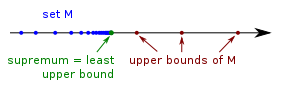
\includegraphics[width=3.92in]{images/math_sup} 

}

\caption{최소상계.}\label{fig:unnamed-chunk-5}
\end{figure}

우리는 최소상계와 최대하계의 극한 또한 생각해 볼 수 있다.

\BeginKnitrBlock{definition}[상극한과 하극한 그리고 극한]
\protect\hypertarget{def:unnamed-chunk-6}{}{\label{def:unnamed-chunk-6} \iffalse (상극한과 하극한 그리고 극한) \fi{} }\(\{ x_{n}\}_{n=1}^{\infty}\)를 실수들의 수열이라고 하자. 수열 \(\{ x_{n}\}_{n=1}^{\infty}\)의 \textbf{상극한(limit supremum)}은
\[\lim_{n\rightarrow\infty}\sup x_{n}=\inf_{n\in\mathbb{N}}\sup_{k\geq n}x_{k}\]
이다. 마찬가지로 수열 \(\{ x_{n}\}_{n=1}^{\infty}\)의 \textbf{하극한(limit infimum)}은
\[\lim_{n\rightarrow\infty}\inf x_{n}=\sup_{n\in\mathbb{N}}\inf_{k\geq n}x_{k}\]
로 정의한다. 만약
\[\lim_{n\rightarrow\infty}\sup x_{n}=\lim_{n\rightarrow\infty}\inf x_{n}=c\in\mathbb{R}\]
일 경우 \(c\)를 수열 \(\{ x_{n}\}_{n=1}^{\infty}\)의 \textbf{극한(limit)}이라고 한다.
\EndKnitrBlock{definition}

\begin{figure}

{\centering 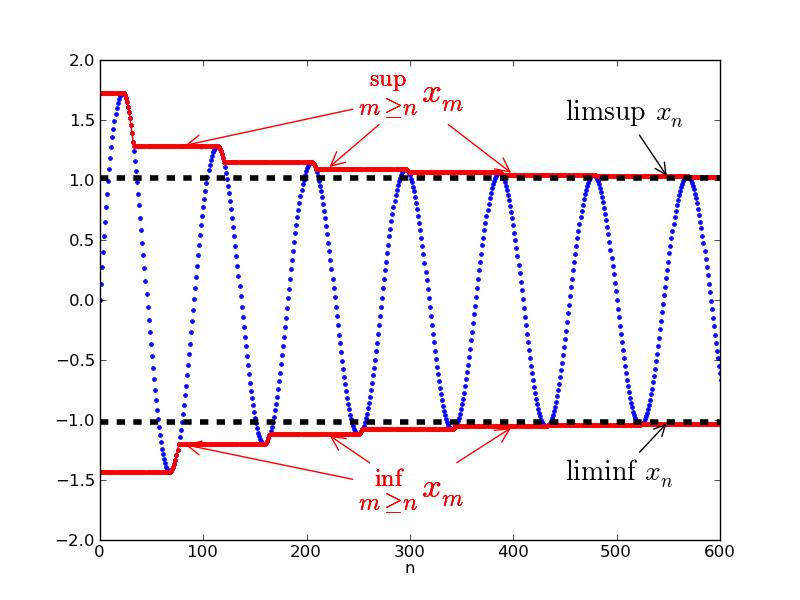
\includegraphics[width=11.11in]{images/math_limsupliminf} 

}

\caption{상극한과 하극한.}\label{fig:unnamed-chunk-7}
\end{figure}

\hypertarget{-operators-and-norms}{%
\section{연산자들과 노름(operators and norms)}\label{-operators-and-norms}}

\hypertarget{direct-sum}{%
\subsection{직합(direct sum)}\label{direct-sum}}

\BeginKnitrBlock{definition}[직합]
\protect\hypertarget{def:unnamed-chunk-8}{}{\label{def:unnamed-chunk-8} \iffalse (직합) \fi{} }크기 \(m \times n\)인 행렬 \(\mathbf{A}\)와 \(p\times q\)인 행렬 \(\mathbf{B}\)가 있을 때 이들의 \textbf{직합(direct sum)}은
\[\mathbf{A}\oplus\mathbf{B}=
\begin{bmatrix}
\mathbf{A} & 0\\
0 & \mathbf{B}\\
\end{bmatrix}
=
\begin{bmatrix}
a_{11} & \cdots & a_{1n} & 0 & \cdots & 0 \\
\vdots & \ddots & \vdots & \vdots & \ddots & \vdots \\
a_{m1} & \cdots & a_{mn} & 0 & \cdots & 0 \\
0 & \cdots & 0 & b_{11} & \cdots & b_{1q} \\
\vdots & \ddots & \vdots & \vdots & \ddots & \vdots \\
0 & \cdots & 0 & b_{p1} & \cdots & b_{pq} \\
\end{bmatrix}
\]
\EndKnitrBlock{definition}

\BeginKnitrBlock{example}[직합의 예]
\protect\hypertarget{exm:unnamed-chunk-9}{}{\label{exm:unnamed-chunk-9} \iffalse (직합의 예) \fi{} }\[
\begin{bmatrix}
1 & 3 & 2\\
2 & 3 & 1\\
\end{bmatrix}
\oplus
\begin{bmatrix}
1 & 6\\
0 & 1\\
\end{bmatrix}
=
\begin{bmatrix}
1 & 3 & 2 & 0 & 0\\
2 & 3 & 1 & 0 & 0\\
0 & 0 & 0 & 1 & 6\\
0 & 0 & 0 & 0 & 1\\
\end{bmatrix}
\]
\EndKnitrBlock{example}

\hypertarget{-kronecker-product}{%
\subsection{크로네커 곱(Kronecker product)}\label{-kronecker-product}}

\BeginKnitrBlock{definition}[크로네커 곱]
\protect\hypertarget{def:unnamed-chunk-10}{}{\label{def:unnamed-chunk-10} \iffalse (크로네커 곱) \fi{} }크기 \(m \times n\)인 행렬 \(\mathbf{A}\)와 \(p\times q\)인 행렬 \(\mathbf{B}\)가 있을 때 이들의 \textbf{크로네커 곱(Kronecker product)}은
\[\mathbf{A}\otimes\mathbf{B}
=
\begin{bmatrix}
a_{11}\mathbf{B} & \cdots & a_{1n}\mathbf{B} \\
\vdots & \ddots & \vdots \\
a_{m1}\mathbf{B} & \cdots & a_{mn}\mathbf{B} \\
\end{bmatrix}
\]
\EndKnitrBlock{definition}

\BeginKnitrBlock{example}[크로네커 곱의 예]
\protect\hypertarget{exm:unnamed-chunk-11}{}{\label{exm:unnamed-chunk-11} \iffalse (크로네커 곱의 예) \fi{} }다음은 크로네커 곱의 한 예이다.

\[
\begin{bmatrix}
1 & 2\\
3 & 4\\
\end{bmatrix}
\otimes
\begin{bmatrix}
0 & 5\\
6 & 7\\
\end{bmatrix}
=
\begin{bmatrix}
1\cdot 0 & 1\cdot 5 & 2\cdot 0 & 2\cdot 5\\
1\cdot 6 & 1\cdot 7 & 2\cdot 6 & 2\cdot 7\\
3\cdot 0 & 3\cdot 5 & 4\cdot 0 & 4\cdot 5\\
3\cdot 6 & 3\cdot 7 & 4\cdot 6 & 4\cdot 7\\
\end{bmatrix}
=
\begin{bmatrix}
0 & 5 & 0 & 10\\
6 & 7 & 12 & 14\\
0 & 5 & 0 & 20\\
18 & 21 & 24 & 28\\
\end{bmatrix}
\]
\EndKnitrBlock{example}

\hypertarget{-kroneckerian-power}{%
\subsection{크로네커 거듭곱(Kroneckerian power)}\label{-kroneckerian-power}}

We call \(p^{k}\)-vector \(\mathbf{a}^{\otimes k}\), the \(k\)-th power of the \(p\)-vector \(\mathbf{a}\), if \(\mathbf{a}^{\otimes 0}=1\) and
\[\mathbf{a}^{\otimes k} = \mathbf{a} \otimes \cdots \otimes\mathbf{a} (\text{ k times}).\]
In general, for any matrix \(\mathbf{A}\), the Kroneckerian power is given by
\[\mathbf{A}^{\otimes k} = \mathbf{A} \otimes \cdots \otimes\mathbf{A} (\text{ k times}).\]
Furthermore, \(\mathbf{A}^{\otimes k}\mathbf{B}^{\otimes k}=(\mathbf{A}\mathbf{B})^{\otimes k}\). In particular, it is noted that
\[\mathbf{a}^{\otimes k}\otimes\mathbf{a}^{\otimes j}= \mathbf{a}^{\otimes (k+ j)}, \qquad{k,j\in\mathbb{N}.}\]
The following statement makes it possible to identify where in a long vector of the Kroneckerian power a certain element of the product is situated.

\hypertarget{tensor-product}{%
\subsection{텐서곱(tensor product)}\label{tensor-product}}

이 부분은 \citep{Kokoszka2017}의 10.5절을 참고하였다. 우리가 covariance operator를 다룰 때 텐서곱과 텐서 공간을 생각하는 것이 편리할 때가 있다고 한다. 특히 무한차원이나 일반적인 힐버트 공간에서는 텐서곱의 활용이 절대적이다.

다음과 같은 행렬 \(\mathbf{A}\in\mathbb{R}^{N\times M}\)을 생각해보자. 이 행렬은 세 가지 방법으로 바라볼 수 있다.

\begin{enumerate}
\def\labelenumi{\arabic{enumi}.}
\item
  전통적인 행렬
\item
  \(\mathbb{R}^{N}\rightarrow\mathbb{R}^{M}\)으로 가는 선형 변환: 벡터의 왼쪽이나 오른쪽에 행렬을 곱하는 형태 (유클리드 공간에서의 모든 선형 변환을 떠올려보자)
\item
  \(\mathbb{R}^{N}\times \mathbb{R}^{M}\rightarrow\mathbb{R}\)인 겹선형(bilinear) functional: 이차 형식에서 많이 다루는 형태이다. 다음과 같이 두 유클리드 공간 \(\mathcal{H}_{1}=\mathbb{R}^{N},\mathcal{H}_{2}=\mathbb{R}^{M}\)가 있다고 하자. 두 개의 벡터 \(x_{1}\in\mathbb{R}^{N}\), \(x_{2}\in\mathbb{R}^{M}\)에 \textbf{텐서곱(tensor product)}를 적용하면 다음과 같은 행렬을 유도한다.
  \[x_{1}\otimes x_{2}:=x_{1}x_{2}^{T}.\]
  또한 공간 \(\mathbb{R}^{N}\otimes \mathbb{R}^{M}\)은 위와 같은 원소들의 모든 유한한 선형 결합의 공간으로 정의할 수 있다. 다시 말하면 만약 \(\mathbf{A}\in\mathbb{R}^{N}\otimes \mathbb{R}^{M}\rightarrow\mathbb{R}\)이면 \(J\)개의 원소들 \(x_{1j}\in\mathbb{R}^{N}\), \(x_{2j}\in\mathbb{R}^{M}\)이 존재해
  \[\mathbf{A}=\sum_{j=1}^{J}x_{1j}\otimes x_{2j}=\sum_{j=1}^{J}x_{1j}x_{2j}^{T}\]
  를 만족한다. 어떤 \(N\times M\) 행렬도 이런 표현 방법으로 표현할 수 있으므로 \(\mathbb{R}^{N}\otimes \mathbb{R}^{M}=\mathbb{R}^{N\times M}\)으로 표현할 수 있다. 이제 이 세번째 관점을 다른 공간에 대해서도 특정화해보자. 어떤 \(N\times M\) 행렬 \(\mathbf{A}\)는 다음과 같은
  \[\mathbf{A}(y_{1},y_{2}):=y_{1}^{T}\mathbf{A}y_{2}\]
  인 겹선형 mapping을 이끌어낸다. 따라서 공간 \(\mathbb{R}^{N}\otimes \mathbb{R}^{M}\)은 모든 겹선형 map \(\mathbb{R}^{N}\times \mathbb{R}^{M}\rightarrow \mathbb{R}\)들의 집합으로 identified될 수 있다. 오브젝트 \(x_{1}\otimes x_{2}\)는 또한 다음과 같은 겹선형 mapping
  \[(x_{1}\otimes x_{2})(y_{1},y_{2})=y_{1}^{T}x_{1}x_{2}^{T}y_{2}=(y_{1}^{T}x_{1})(y_{2}^{T}x_{2})\]
  로 identified될 수 있다.
\end{enumerate}

이러한 관점에서 텐서를 바라보자. 텐서는 스칼라들의 체가 연관된 공간에서의 cartesian 곱으로부터 오는 다중선형사상(multilinear map)이다. 만약 \(\{e_{1j} \}\)와 \(\{e_{2j} \}\)가 \(\mathbb{R}^{N}\)과 \(\mathbb{R}^{M}\)의 정규 기저들이라고 하자. 그러면 \(\{e_{1j}\otimes e_{2j} \}\)는 \(\mathbb{R}^{N}\times \mathbb{R}^{M}\)의 기저가 된다. 이런 방식으로 우리는 이 기저를 전통적인 행렬에도 적용할 수 있다.
\[\mathbf{A}(e_{1j}^{T}, e_{2k})=e_{1j}^{Y}\mathbf{A}e_{2k}=\mathbf{A}(j,k).\]

\BeginKnitrBlock{definition}[힐버트 공간에서의 텝서곱]
\protect\hypertarget{def:unnamed-chunk-12}{}{\label{def:unnamed-chunk-12} \iffalse (힐버트 공간에서의 텝서곱) \fi{} }\(x_{1}\in\mathcal{H}_{1}\)과 \(x_{2}\in\mathcal{H}_{2}\)를 두 실 힐버트 공간에서의 원소들이라고 하자. 그러면 텐서곱 \(x_{1}\otimes x_{2}: \mathcal{H}_{1}\times\mathcal{H}_{2} \rightarrow\mathbb{R}\)은 겹선형 사상으로 어떤 \((y_{1},y_{2})\times \mathcal{H}_{1}\times \mathcal{H}_{2}\)에 대해
\[(x_{1}\otimes x_{2})(y_{1},y_{2})=\langle x_{1},y_{1}\rangle_{\mathcal{H}_{1}}\langle x_{2},y_{2}\rangle_{\mathcal{H}_{2}}\]
로 정의된다.
\EndKnitrBlock{definition}

\BeginKnitrBlock{example}[행렬의 텐서곱 예시]
\protect\hypertarget{exm:unnamed-chunk-13}{}{\label{exm:unnamed-chunk-13} \iffalse (행렬의 텐서곱 예시) \fi{} }\[
\begin{bmatrix}
1 & 2\\
3 & 4
\end{bmatrix}
\otimes
\begin{bmatrix}
1 & 1 & 1\\
1 & 1 & 1\\
1 & 1 & 2
\end{bmatrix}
=
\begin{bmatrix}
1 & 1 & 1 & 2 & 2 & 2\\
1 & 1 & 1 & 2 & 2 & 2\\
1 & 1 & 2 & 2 & 2 & 4\\
3 & 3 & 3 & 4 & 4 & 4\\
3 & 3 & 3 & 4 & 4 & 4\\
3 & 3 & 6 & 4 & 4 & 8\\
\end{bmatrix},
\]
\[
\begin{bmatrix}
1 & 1 & 1\\
1 & 1 & 1\\
1 & 1 & 2
\end{bmatrix}
\otimes
\begin{bmatrix}
1 & 2\\
3 & 4
\end{bmatrix}
=
\begin{bmatrix}
1 & 2 & 1 & 2 & 1 & 2\\
3 & 4 & 3 & 4 & 3 & 4\\
1 & 2 & 1 & 2 & 1 & 2\\
3 & 4 & 3 & 4 & 3 & 4\\
1 & 2 & 1 & 2 & 2 & 4\\
3 & 4 & 3 & 4 & 6 & 8\\
\end{bmatrix}.
\]
\EndKnitrBlock{example}

\hypertarget{-cartesian-product}{%
\subsection{데카르트 곱(Cartesian product)}\label{-cartesian-product}}

두 개의 집합 \(A\), \(B\)가 있을 때, 이들의 \textbf{데카르트 곱(Cartesian product)} \(A\times B\)는
\[A\times B = \{ (a,b)| a\in A \text{ and } b \in B\}\]
로 정의된다.

\hypertarget{norm}{%
\subsection{노름(norm)}\label{norm}}

\hypertarget{-vector-norm}{%
\subsubsection{벡터 노름(vector norm)}\label{-vector-norm}}

\BeginKnitrBlock{definition}[노름과 노름공간]
\protect\hypertarget{def:unnamed-chunk-14}{}{\label{def:unnamed-chunk-14} \iffalse (노름과 노름공간) \fi{} }벡터공간 \(X\)에서 다음 세 조건들이 만족되면 함수 \(\|\cdot\|\)을 \textbf{노름(norm)}이라 하고 또한 벡터공간 \(X\)를 \textbf{노름공간(normed space)}라 한다.

\begin{enumerate}
\def\labelenumi{\arabic{enumi}.}
\item
  임의의 \(\mathbf{x}\in X\), where \(\|\mathbf{x}\| \geq 0\)이며 \(\|\mathbf{x}\|=0\)이기 위한 필요충분조건은 \(\mathbf{x}=\mathbf{0}\)이다.
\item
  임의의 \(\mathbf{x}, \mathbf{y}\in X\)에 대해
  \[\| \mathbf{x}+\mathbf{y}\|\leq \|\mathbf{x}\| + \|\mathbf{y}\|\]
  가 성립한다.
\item
  임의의 스칼라 \(\alpha\)와 임의의 \(\mathbf{x}\in X\)에 대해
  \[\| \alpha \mathbf{x}\|=|\alpha| \|\mathbf{x}\|\]
  가 성립한다.
\end{enumerate}
\EndKnitrBlock{definition}

\hypertarget{-matrix-norm}{%
\subsubsection{행렬 노름(matrix norm)}\label{-matrix-norm}}

\hypertarget{-matrix-decomposition}{%
\section{행렬의 분해(matrix decomposition)}\label{-matrix-decomposition}}

\hypertarget{-eigenvalue-decomposition}{%
\subsection{고유값 분해(eigenvalue decomposition)}\label{-eigenvalue-decomposition}}

고유값 분해는 행렬 \(A\)가 \(n\times n\) 정방행렬일 때만 적용 가능하다.

\hypertarget{spectraldecomposition}{%
\subsection{스펙트럼 분해(spectral decomposition)}\label{spectraldecomposition}}

\(p\times p\) 대칭행렬 \(A\)에 대한 \textbf{스펙트럼 분해(spectral decomposition)}는 다음과 같다. \(p\times p\) 대칭행렬 \(A\)는 직교행렬 \(P\)에 의해 \textbf{대각화(diagonalization)}된다고 한다.

\[A=P\Lambda P^{T}=\sum_{i=1}^{p}\lambda_{i}e_{i}e_{i}^{T}.\]

이때 \(PP^{T}=P^{T}P=I\)를 만족하는 직교행렬 \(P\)는 \(P=[e_{1},\ldots , e_{p}]\)로 이루어지며, \(\Lambda\)는 \(A\)의 고유값(eigenvalue)들로만 이루어진 대각행렬(diagonal matrix)

\[
\Lambda=
\begin{bmatrix}
\lambda_{1} & \cdots & 0\\
\vdots & \ddots & \vdots\\
0 & \cdots & \lambda_{p}\\
\end{bmatrix}
\]

이다. 대각행렬 \(\Lambda\)는 \(P^{T}AP=\Lambda\)이다.

\hypertarget{svd}{%
\subsection{특이값분해(SVD)}\label{svd}}

\textbf{특이값분해(singular value decomposition, SVD)}는 \(m\times n\) 직사각형 행렬 \(A\)에 대해 스펙트럼 분해를 일반화한 것이다.
\(A\)의 특이값 분해는 다음과 같다.

\[A=U\Sigma V^{T}.\]

이 때

\begin{itemize}
\item
  \(U\): \(A\)의 left singular vector로 이루어진 \(m\times m\) 직교행렬(orthogonal matrix)
\item
  \(\Sigma\): 주 대각성분이 \(\sqrt{\lambda_{i}}\)로 이루어진 \(m\times n\) 직사각 대각행렬(diagonal matrix)
\item
  \(V\): \(A\)의 right singular vector로 이루어진 \(n\times n\) 직교행렬(orthogonal matrix)
\end{itemize}

행렬 \(A\)의 계수(rank)가 \(k\)라고 할 때,

\begin{itemize}
\item
  \(U=[u_{1},\ldots , u_{k}, \ldots u_{m}]\)는 \(AA^{T}\)를 고유값분해(eigenvalue decomposition)로 직교대각화하여 얻은 \(m\times m\) 직교행렬(orthogonal matrix)이며, 특히 \([u_{1},\ldots, u_{k}]\)를 \textbf{좌특이벡터(left signular vector)}라고 한다.
\item
  \(V=[v_{1},\ldots ,v_{k},\ldots , v_{n}]\)는 \(A^{T}A\)를 고유값분해로 직교대각화하여 얻은 \(n\times n\) 직교행렬이며, 특히 \([v_{1},v_{2},\ldots ,v_{k}]\)를 \textbf{우특이벡터(right signular vector)}라고 한다.
\item
  \(\Sigma\)는 \(A^{T}A\)의 0이 아닌 고유값이 \(\lambda_{1},\lambda_{2},\ldots , \lambda_{k}\)일 때 \(\sqrt{\lambda_{1}},\ldots, \sqrt{\lambda_{k}}\)를 대각성분으로 가지고 나머지 성분을 0으로 갖는 \(m\times n\) 직사각 \textbf{대각행렬(diagonal matrix)}이다.
\end{itemize}

\[
\Sigma=
\begin{bmatrix}
\sqrt{\lambda_{1}} & 0 & \cdots & 0 & 0 & \cdots & 0\\
0 & \sqrt{\lambda_{2}} & \cdots & 0 & 0 & \cdots & 0\\
\vdots & \vdots & \ddots & \vdots & \vdots & \cdots & 0\\
0 & 0 & \cdots & \sqrt{\lambda_{k}} & 0 & \cdots & 0\\
0 & 0 & 0 & 0 & 0 & \cdots & 0\\
\vdots & \vdots & \vdots & \vdots & \vdots & \ddots & \vdots\\
0 & 0 & 0 & 0 & 0 & \cdots & 0\\
\end{bmatrix}.
\]

즉 \(A\)를 다시 쓰면

\[
A=
\begin{bmatrix}
u_{1} & \cdots & u_{k} & \cdots & u_{m}\\
\end{bmatrix}
\begin{bmatrix}
\sqrt{\lambda_{1}} & 0 & \cdots & 0 & 0 & \cdots & 0\\
0 & \sqrt{\lambda_{2}} & \cdots & 0 & 0 & \cdots & 0\\
\vdots & \vdots & \ddots & \vdots & \vdots & \cdots & 0\\
0 & 0 & \cdots & \sqrt{\lambda_{k}} & 0 & \cdots & 0\\
0 & 0 & 0 & 0 & 0 & \cdots & 0\\
\vdots & \vdots & \vdots & \vdots & \vdots & \ddots & \vdots\\
0 & 0 & 0 & 0 & 0 & \cdots & 0\\
\end{bmatrix}
\begin{bmatrix}
V_{1}^{T}\\
\vdots \\
V_{k}^{T}\\
\vdots\\
V_{n}^{T}\\
\end{bmatrix}
\]

이다. 위 식에서 \textbf{특이값(singular value)}는 \(\sigma_{i}^{2}=\lambda_{i}\)로부터 \(\sigma_{i}=\sqrt{\lambda_{i}}\)가 된다. 참고로 \(U, V\)가 직교행렬이면 \(UU^{T}=I\), \(VV^{T}=I\)가 성립한다.

\hypertarget{--the-relationship-between-spectral-decomposition-and-eigenvalue-decomposition}{%
\subsection{특이값분해와 고유값분해의 관계(the relationship between spectral decomposition and eigenvalue decomposition)}\label{--the-relationship-between-spectral-decomposition-and-eigenvalue-decomposition}}

\(m\times n\) 행렬 \(A\)의 특이값분해의 \(U\)는 \(AA^{T}\)의 고유벡터이고, \(V\)는 \(A^{T}A\)의 고유벡터이며, \(A\)의 0이 아닌 특이값들의 제곱 \(\Sigma\Sigma^{T}, \Sigma^{T}\Sigma\)는 \(AA^{T}\), \(A^{T}A\)의 고유값과 같음을 알 수 있다. 참고로 \(\sigma_{i}=\sqrt{\lambda_{i}}\) 이므로 \(\Sigma\Sigma^{T}\) 또는 \(\Sigma^{T}\Sigma=\lambda_{i}\)이다.

\begin{eqnarray*}
U&=&AA^{T}\\
&=&(U\Sigma V^{T})(U\Sigma V^{T})^{T}\\
&=&(U\Sigma V^{T})(V\Sigma^{T} U^{T})\\
&=&U(\Sigma\Sigma^{T})U^{T}\\
\end{eqnarray*}

\begin{eqnarray*}
V&=&A^{T}A\\
&=&(U\Sigma V^{T})^{T}(U\Sigma V^{T})\\
&=&(V\Sigma^{T} U^{T})(U\Sigma V^{T})\\
&=&V(\Sigma^{T}\Sigma)V^{T}\\
\end{eqnarray*}

즉 \(u_{1},\ldots , u_{k}, \ldots u_{m}\)는 range\((A)\)의 직교정규벡터, \(v_{1},\ldots ,v_{k},\ldots , v_{n}\)는 \(\mathcal{N}(A)^{\perp}\)의 직교정규벡터이다.

\hypertarget{----additional-explanation-about-spectral-decomposition}{%
\subsection{특이값 분해에 대한 추가 설명(additional explanation about spectral decomposition)}\label{----additional-explanation-about-spectral-decomposition}}

여기서는 \href{https://web.stanford.edu/class/archive/ee/ee263/ee263.1082/notes/ee263coursereader.pdf}{Boyd 교수의 강의노트}를 참고하였다. 잠시 편의를 위해 \(U\) 는 \(m\times n\) 행렬, \(\Sigma\)는 \(n \times n\) 행렬이라고 하자. 그러면 특이값 분해는

\[A=U\Sigma V^{T}=\sum_{i=1}^{n}\sigma_{i}u_{i}v_{i}^{T}\]

\begin{figure}

{\centering 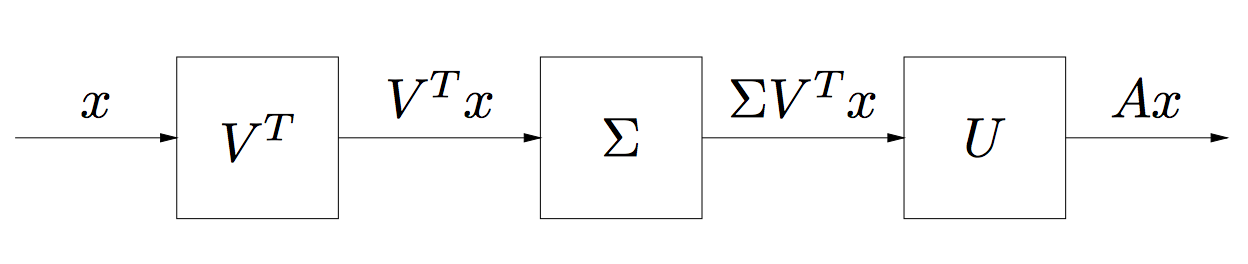
\includegraphics[width=17.33in]{images/math_svd001} 

}

\caption{SVD 그림.}\label{fig:unnamed-chunk-15}
\end{figure}

가 된다. 선형 사상(mapping) \(y=Ax\)는 다음과 같이 분해할 수 있다.

\begin{itemize}
\item
  \(x\)를 input direction들 \(v_{1}, \ldots , v_{n}\)을 따라 계수들을 계산한다.
\item
  \(\sigma_{i}\)는 척도계수
\item
  이것들을 다시 output directions \(u_{1}, \ldots, u_{n}\)을 따라 재구성한다.
\end{itemize}

대칭행렬 \(A\)에 대한 고유값 분해와 달라지는 점은 input direction들과 output direction들이 다르다는 것이다.

\begin{itemize}
\item
  \(v_{1}\)는 input direction으로 가장 민감하다.(most sensitive, highest gain)
\item
  \(u_{1}\)은 output direction으로 가장 민감하다.
\item
  \(Av_{1}=\sigma_{1}u_{1}\)이다.
\end{itemize}

\BeginKnitrBlock{example}[SVD의 기하학적 의미 예]
\protect\hypertarget{exm:unnamed-chunk-16}{}{\label{exm:unnamed-chunk-16} \iffalse (SVD의 기하학적 의미 예) \fi{} }\(A=\mathbb{R}^{2\times 2}\)이며 \(\Sigma=\text{diag}(1,0.5)\)인 경우를 생각해보자. 이 경우 \(x\)를 \(v_{1}\), \(v_{2}\)를 따라 풀면 \(v_{1}^{T}x=0.5, v_{2}^{T}x=0.6\) 즉 \(x=0.5v_{1} + 0.6v_{2}\)이며, \(Ax=(v_{1}^{T}x)\sigma_{1}u_{1} + (v_{2}^{T}x)\sigma_{2}u_{2}= (0.5)(1)u_{1} + (0.6)(0.5)u_{2}\) 이다.
\EndKnitrBlock{example}

\begin{figure}

{\centering 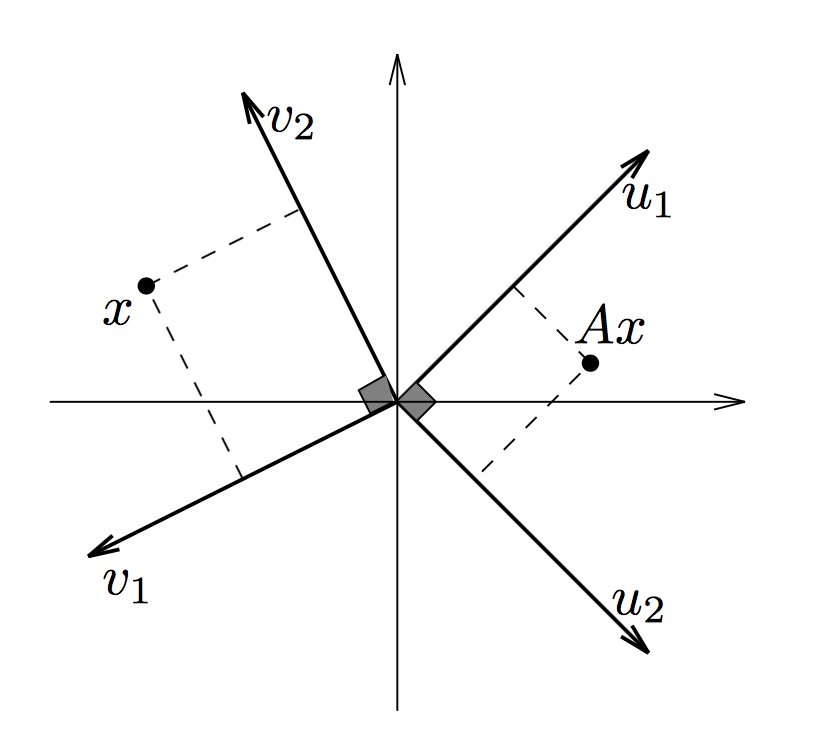
\includegraphics[width=11.5in]{images/math_svd002} 

}

\caption{SVD 예제 그림.}\label{fig:unnamed-chunk-17}
\end{figure}

\hypertarget{---geometrical-meaning-of-spectral-decomposition}{%
\subsection{특이값 분해의 기하학적 의미(geometrical meaning of spectral decomposition)}\label{---geometrical-meaning-of-spectral-decomposition}}

\href{https://en.wikipedia.org/wiki/Singular_value_decomposition}{위키피디아}를 참고하자.

\hypertarget{basis}{%
\section{기저(basis)}\label{basis}}

\hypertarget{-riesz-basis}{%
\subsection{리츠 기저(Riesz basis)}\label{-riesz-basis}}

In the Hilbert space \(L_{2}[0,1]\), an unconditional basis is called a \textbf{Riesz basis} if it is ``almost normalized''. This means that there exist real, positive, non-zero consts \(m\) and \(M\) so that
\[0 < m \leq \| \phi_{i}\|\leq M < \infty.\]
A Riesz basis is characterized by two Riesz constants \(A\) and \(B\), so that for all \(f=\sum_{i}s_{i}\phi_{i}\in L_{2}[0,1]\),
\[A^{2}\| f \|^{2}\leq \sum_{i\in\mathbb{Z}}s_{i}^{2}\leq B^{2}\|f\|^{2}.\]

(Jensen의 Noise reduction and wavelet thresholding으로부터)

There exists \(\phi_{0}(x)\in\mathcal{V}_{1}\) such that \(\{ \phi_{0}(x-k) | k\in\mathcal{Z} \}\) forms a Riesz basis of \(\mathcal{V}_{1}\), i.e, there exists \(0< A \leq B <\infty\) such that
\[A \| c_{k}\|^{2} \leq \| \sum_{k}c_{k}\phi_{0}(x-k)\|^{2} \leq B \| c_{k} \|^{2}\]
for all \(\{c_{k}\}\in l^{2}\), where \(A\) and \(B\) do not depend on the \(c_{k}\)

(동익이형 박사논문 47쪽)

\hypertarget{radial-basis-function}{%
\subsection{Radial basis function}\label{radial-basis-function}}

Radial funtion이란 거리에만 의존하는 함수를 의미한다. 어떤 함수에 대한 근사 모델을 radial function의 선형조합으로 표현할 수 있다.

\begin{itemize}
\tightlist
\item
  Gaussian
\end{itemize}

\[\phi(r)=e^{-(\epsilon r)^{2}}\]

\begin{itemize}
\tightlist
\item
  Multiquadric
\end{itemize}

\[\phi(r)=\sqrt{1+(\epsilon r)^{2}}\]

\begin{itemize}
\tightlist
\item
  Inverse quadratic
\end{itemize}

\[\phi(r)=\frac{1}{1+(\epsilon r)^{2}}\]

\begin{itemize}
\tightlist
\item
  Inverse multiquadric
\end{itemize}

\[\phi(r)=\frac{1}{\sqrt{1+(\epsilon r)^{2}}}\]

\hypertarget{space}{%
\section{공간(space)}\label{space}}

이 부분은 전체적으로 \citep{Shima2016}의 정의와 내용들을 따라간다.

\hypertarget{-groups-and-fields}{%
\subsection{군과 장(groups and fields)}\label{-groups-and-fields}}

수학에서 \textbf{군(group)}은 연산과 함께 정의되는 원소들의 집합으로 원소들이 closure, associativity, identity and invertability를 만족해야 한다. 대충 말해서 \textbf{장(field)}은 합, 차, 곱, 몫의 개념을 갖고 있는 대수적 구조이다.

\hypertarget{-vector-spaces}{%
\subsection{벡터 공간(vector spaces)}\label{-vector-spaces}}

벡터 공간은 스칼라들의 장(field)에서 정의된다. 이런 스칼라들은 실수가 될 수도 있고, 복소수가 될 수도 있다. 벡터 공간은 덧셈과 곱셈을 적용할 수 있는 수학적 실재(mathematical entity)들의 집합이다. 예를 들면 숫자 공간 \(\mathbb{R}\), \(\mathbb{C}\) 등은 벡터 공간이 된다. 숫자 뿐만 아니라 함수, 다항식, 선형 연산자, 벡터 등등이 수학적 실재가 될 수 있다.

\begin{figure}

{\centering 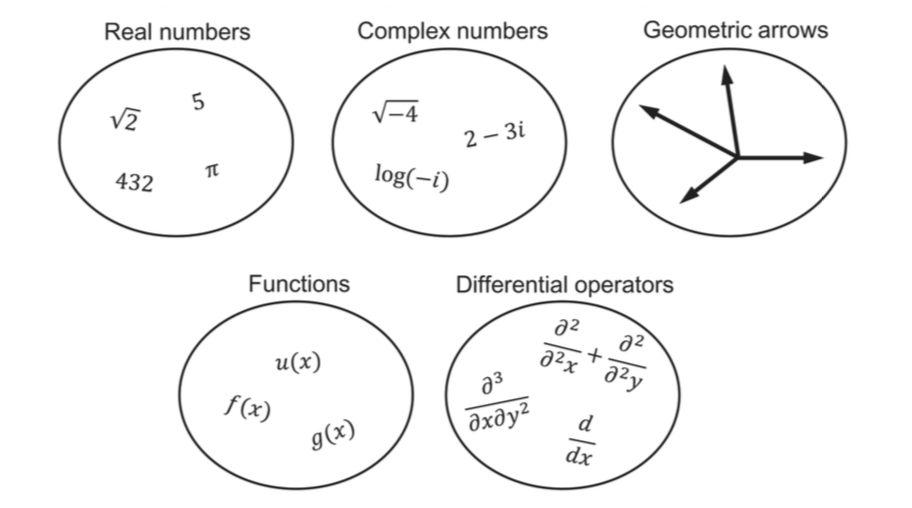
\includegraphics[width=12.67in]{images/math_vectorspace} 

}

\caption{벡터 공간은 다양한 종류의 수학적 실재(mathematical entity)로부터 만들어진다.}\label{fig:unnamed-chunk-18}
\end{figure}

\textbf{벡터 공간(vector space)} \(V\)는 다음 공리들을 만족하는 원소들 \(\mathbf{x}\) (벡터라 부른다)의 collection이다.

\begin{enumerate}
\def\labelenumi{\arabic{enumi}.}
\tightlist
\item
  \(V\)는 덧셈 하에서 교환 가능한 가환군(commutative group, 교환 법칩이 성립하는 군)이다.

  \begin{enumerate}
  \def\labelenumii{\roman{enumii}.}
  \tightlist
  \item
    \(\mathbf{x}+\mathbf{y}=\mathbf{y}+\mathbf{x}\in V\) for any \(\mathbf{x},\mathbf{y}\in V\) (closure)
  \item
    \(\mathbf{x} + (\mathbf{y}+\mathbf{z}) = (\mathbf{x} + \mathbf{y}) + \mathbf{z}\in V\) for any \(\mathbf{x},\mathbf{y}, \mathbf{z}\in V\) (associativity)
  \item
    다음과 같은 \(\mathbf{0}\)벡터(항등원)가 존재해 모든 \(\mathbf{x}\in V\)에 대해 \(\mathbf{x}+\mathbf{0}=\mathbf{x}\)를 만족한다. (identity)
  \item
    다음과 같은 덧셈에 대한 역원 \(-\mathbf{x}\)이 존재해 \(\mathbf{x}+(-\mathbf{x})=\mathbf{0}\)이 된다. (invertibility)
  \end{enumerate}
\item
  \(V\)는 어떤 장 \(\mathbb{F}\)에 대해 다음의 공리를 만족하며, 이런 원소들을 \textbf{스칼라(scalar)}라고 부른다.

  \begin{enumerate}
  \def\labelenumii{\roman{enumii}.}
  \tightlist
  \item
    \(V\)는 스칼라 곱에 대해 닫혀 있다.
    \[\alpha \mathbf{x} \in V \text{ for arbitrary } \mathbf{x} \in V, \alpha \in \mathbb{F}.\]
  \item
    스칼라 곱은 \(V\)와 \(\mathbb{F}\)의 원소들에 대해 \textbf{분배가능(distributive)}하다.
    \[\alpha(\mathbf{x}+\mathbf{y})=\alpha\mathbf{x}+ \alpha\mathbf{y}\in V, (\alpha+\beta)\mathbf{x}=\alpha\mathbf{x}+\beta\mathbf{y}\in V.\]
  \item
    스칼라 곱은 결합법칙이 성립한다. \(\alpha(\beta\mathbf{x})=\beta(\alpha \mathbf{x}).\)
  \item
    Zero scalar \(0\in\mathbb{F}\)에 대한 곱은 항등원 \(0\mathbf{x}=\mathbf{0}\in V\)을 생산한다.
  \item
    Unit scalar \(1 \in \mathbb{F}\)는 \(1\mathbf{x}=\mathbf{x}\) 성질을 갖는다.
  \end{enumerate}
\end{enumerate}

여기서부터는 벡터 공간의 주요 성질들에 대해 다룬다.

\hypertarget{inner-products}{%
\subsection{내적(inner products)}\label{inner-products}}

\BeginKnitrBlock{definition}[내적]
\protect\hypertarget{def:unnamed-chunk-19}{}{\label{def:unnamed-chunk-19} \iffalse (내적) \fi{} }내적은 \(\mathbf{x}\), \(\mathbf{y}\)의 순서쌍을 스칼라(좀 더 일반적으로는 복소수)에 mapping하는 것이고 \(\langle\mathbf{x},\mathbf{y}\rangle\)로 쓴다. 이 mapping은 다음 규칙들을 만족해야 한다.

\begin{enumerate}
\def\labelenumi{\arabic{enumi}.}
\item
  \(\langle\mathbf{x},\mathbf{y}\rangle = \langle\mathbf{y},\mathbf{x}\rangle^{*}\). (여기서 별표는 complex conjugate를 의미한다.)
\item
  \(\langle\alpha\mathbf{x}+\beta\mathbf{y}, \mathbf{z}\rangle = \alpha^{*}\langle\mathbf{x},\mathbf{z}\rangle+\beta^{*}\langle\mathbf{y},\mathbf{z}\rangle\) (여기서 \(\alpha\), \(\beta\)는 어떤 복소수이다.)
\item
  모든 \(\mathbf{x}\)에 대해 \(\langle\mathbf{x},\mathbf{x}\rangle \geq 0\)이다.
\item
  \(\langle\mathbf{x},\mathbf{x}\rangle = 0\)은 \(\mathbf{x}=\mathbf{0}\)과 필요충분조건이다.
\end{enumerate}
\EndKnitrBlock{definition}

특별히 내적을 갖고 있는 벡터 공간을 \textbf{내적 공간(inner product space)}이라고 부른다.

내적 공간에서는 우리는 항상 \textbf{내적 노름(inner product norm)}을 다음과 같이 정의할 수 있다.
\[\|x\|=\sqrt{\langle x,x\rangle}.\]

\BeginKnitrBlock{proposition}[내적 공간의 노름과 관련된 성질들]
\protect\hypertarget{prp:unnamed-chunk-20}{}{\label{prp:unnamed-chunk-20} \iffalse (내적 공간의 노름과 관련된 성질들) \fi{} }내적 공간은 그 공간 상에서 노름 \(\| \cdot \|\)을 정의하며 다음의 설질들을 갖는다.

\begin{itemize}
\item
  \(\|ax\|=|a|\|x\|\)
\item
  \(|\langle x,y\rangle | \leq \|x\| \|y\|\) (Cauchy-Schwarz inequality)
\item
  \(\|x+y\| \leq \|x\| +\|y\|\) (triangle inequality)
\item
  \(d(x,y) = \|x-y\|\) is a metric (distance), i.e., \(d(x,y)=d(y,x)>0\) if \(x\neq y\), \(d(x,x)=0\) and \(d(x,y) \leq d(x,z) + d(z,y)\).
\end{itemize}
\EndKnitrBlock{proposition}

\hypertarget{orthogonality}{%
\subsection{직교성(orthogonality)}\label{orthogonality}}

다음은 \citep{Shima2016}책에 있는 직교성의 정의다.

\BeginKnitrBlock{definition}[직교]
\protect\hypertarget{def:unnamed-chunk-21}{}{\label{def:unnamed-chunk-21} \iffalse (직교) \fi{} }내적 공간에 있는 두 원소들 \(\mathbf{x}, \mathbf{y}\)는 \(\langle x\mathbf{x},\mathbf{y}\rangle = 0\)일 때 \textbf{직교(orthogonal)}한다고 말한다.
\EndKnitrBlock{definition}

\hypertarget{--complete-vector-spaces}{%
\subsubsection{완비 벡터 공간(complete vector spaces)}\label{--complete-vector-spaces}}

벡터 공간이 유한차원일 때, 공간의 완비성(completeness)은 같은 공간의 다른 larger orthonormal set에 포한되어 있지 않는 orthonormal set을 찾음으로써 증명할 수 있다. 예를 들면 3차원 공간에서는 linear combination이 그 공간의 모든 벡터를 표현할 수 있는 three orthonormal vector의 set을 찾기만 하면 되는 것이다. 그러나 우리가 무한 차원 공간을 고려할 때, 무한한 숫자의 orthonormal vector를 고려하는 것은 쉽지 않다. 사실 무한한 숫자의 vector의 linear combination은 때대로 같은 공간에 포함된 벡터를 표현하는 데 충분치 않을 수도 있다. 이러한 모호함을 해결하기 위해 무한 차원 공간에서 완비성을 생각하는 것이다.

\BeginKnitrBlock{definition}[벡터의 Cauchy sequence]
\protect\hypertarget{def:unnamed-chunk-22}{}{\label{def:unnamed-chunk-22} \iffalse (벡터의 Cauchy sequence) \fi{} }벡터의 수열 \(\{ \mathbf{x}_{1},\mathbf{x}_{2},\ldots \}\)가 모든 \(\epsilon >0\)에 대해 적단한 근사 숫자 \(N\)이 존재해 모든 \(m,n > N\)에 대해 \(\| \mathbf{x}_{m} -\mathbf{x}_{n} \| < \epsilon\)을 만족한다면 이를 벡터의 \textbf{코시 수열(Cauchy sequence)}이라고 한다. 쉽게 얘기하자면 \(\mathbf{x}_{m}\)과 \(\mathbf{x}_{n}\)이 \(m,n \rightarrow \infty\) 함체 따라 가까어지는 수열을 코시 수열이라 부르는 것이다.
\EndKnitrBlock{definition}

\BeginKnitrBlock{definition}[코시 수열의 수렴]
\protect\hypertarget{def:unnamed-chunk-23}{}{\label{def:unnamed-chunk-23} \iffalse (코시 수열의 수렴) \fi{} }벡터의 무한 수열 \(\{\mathbf{x}_{1},\mathbf{x}_{2}, \ldots \}\)가 있을 때, 만약 \(\mathbf{x}\)가 존재해 \(\| \mathbf{x}_{n} -\mathbf{x}\|\rightarrow 0\)을 만족한다면 이 수열이 수렴(convergent)한다고 한다.
\EndKnitrBlock{definition}

그러나 그 역은 성립하지 않는다. 코시 수열이라고 해서 다 수렴하는 건 아니다. 완비성을 정의해 이를 해결할 수 있는 것이다.

\BeginKnitrBlock{definition}[벡터 공간의 완비성]
\protect\hypertarget{def:unnamed-chunk-24}{}{\label{def:unnamed-chunk-24} \iffalse (벡터 공간의 완비성) \fi{} }만약 어떤 벡터 공간의 모든 코시 수열이 수렴한다면, 우리는 그 공간을 \textbf{완비(complete)}라고 부른다.
\EndKnitrBlock{definition}

다음은 \citep{Kokoszka2017}의 10장에 나오는 예이다.

\BeginKnitrBlock{example}[유클리드 공간에서의 완비성]
\protect\hypertarget{exm:unnamed-chunk-25}{}{\label{exm:unnamed-chunk-25} \iffalse (유클리드 공간에서의 완비성) \fi{} }유클리드 거리 하에서 개구간 \((0,1)\)은 complete metric space가 아니지만, 닫힌 구간 \([0,1]\)은 complete metric space가 된다. 유클리드 공간 \(\mathbb{R}^{d}\)는 complete하다.
\EndKnitrBlock{example}

\hypertarget{topological-space}{%
\subsection{위상공간(topological space)}\label{topological-space}}

\hypertarget{--separable-space}{%
\subsection{분해 가능 공간(separable space)}\label{--separable-space}}

Countable dense subset을 포함하는 위상공간(topological space)을 \textbf{분해 가능 공간(separable space)}이라고 한다.

\hypertarget{-normed-space}{%
\subsection{노름 공간(normed space)}\label{-normed-space}}

\BeginKnitrBlock{definition}[노름 공간]
\protect\hypertarget{def:unnamed-chunk-26}{}{\label{def:unnamed-chunk-26} \iffalse (노름 공간) \fi{} }원소들에 일종의 `길이' 또는 '크기'가 부여된 벡터 공간 \(V\)을 \textbf{노름 공간(normed space)}라고 한다. 노름은 벡터 공간 \(V\) 위에서의 실수 함수로 \(\| \|\)로 표시하며

\begin{enumerate}
\def\labelenumi{\arabic{enumi}.}
\item
  모든 \(\lambda\in\mathbb{F}\)와 \(x\in V\)에 대해 \(\|\lambda \mathbf{x}\| = |\lambda|\|\mathbf{x}\|\)
\item
  \$\textbar{}\mathbf{x} +\mathbf{y}\textbar{} \leq \textbar{}\mathbf{x}\textbar{} +\textbar{}\mathbf{y}\textbar{}\#
\item
  \(\|\mathbf{x}\|=0\)이라는 것은 \(\mathbf{x}=0\)과 동치다.
\end{enumerate}
\EndKnitrBlock{definition}

노름 공간에 있는 모든 원소들은 항상 유한한 노름을 갖아야 한다. 만약 무한한 노름을 갖는다면 그것은 공간이 될 수 없다. 노름 \(\|\cdot\|\)은 항상 계량(metric)을 유도한다. 계량은 \(\mathcal{F}\)에서의 거리 개념이다. 즉 \(d(f,g)=\| f-g\|_{\mathcal{F}}\)이다. 이것은 \(\mathcal{F}\)가 어떤 위상 구조를 갖고있다는 뜻도 되며 우리는 \(\mathcal{F}\)의 원소들의 수열들이 정의된 거리에서 수렴하는지, 또는 연속 등에 대해서 생각할 수 있게 한다.

\hypertarget{-banach-space}{%
\subsection{바나흐 공간(Banach space)}\label{-banach-space}}

\BeginKnitrBlock{definition}[힐버트 공간]
\protect\hypertarget{def:unnamed-chunk-27}{}{\label{def:unnamed-chunk-27} \iffalse (힐버트 공간) \fi{} }Normed space가 complete일 경우 이를 \textbf{바나흐 공간(Banach space)}라고 부른다.
\EndKnitrBlock{definition}

유한차원에서 노름공간은 항상 완비(complete)이다. 그러나 무한차원에서 노름공간은 완비일 수도 있고, 아닐 수도 있다.

\BeginKnitrBlock{definition}[원-힐버트 공간]
\protect\hypertarget{def:unnamed-chunk-28}{}{\label{def:unnamed-chunk-28} \iffalse (원-힐버트 공간) \fi{} }Inner product spaces들 중 완비가 아닌 공간들을 \textbf{원-힐버트 공간(pre-Hilbert space)}라고 부른다.
\EndKnitrBlock{definition}

\BeginKnitrBlock{example}[원-힐버트 공간의 예]
\protect\hypertarget{exm:unnamed-chunk-29}{}{\label{exm:unnamed-chunk-29} \iffalse (원-힐버트 공간의 예) \fi{} }유클리드 거리 하에서 개구간 \((0,1)\)은 complete metric space가 아니지만, 닫힌 구간 \([0,1]\)은 complete metric space가 된다. 유클리드 공간 \(\mathbb{R}^{d}\)는 complete하다.
\EndKnitrBlock{example}

\hypertarget{-hilbert-space}{%
\subsection{힐버트 공간(Hilbert space)}\label{-hilbert-space}}

많은 함수자료분석은 힐버트 공간 이론에 많이 의존한다. 모든 힐버트 공간은 함수가 무한차원 공간의 점으로서 간주될 수 있도록 하는 수단을 제공해 준다. 이런 기하학적인 관점의 쓰임새는 우리가 기초 선형대수에서 정의했던 길이, 직교정규, 그리고 원소들의 선형 결합 개념들을 좀 더 추상적인 수학적 공간에 일반화시킬 수 있다는 것이다. 이런 기하학적 관점에 가장 핵심이 되는 개념은 공간의 \textbf{기저(basis)}다. 힐버트 공간과 함께, 무한차원 공간에서 기저의 기초적 성질들을 복습해 보기로 한다.

\BeginKnitrBlock{definition}[힐버트 공간]
\protect\hypertarget{def:unnamed-chunk-30}{}{\label{def:unnamed-chunk-30} \iffalse (힐버트 공간) \fi{} }A complete normed space endowed with inner product is called a \textbf{Hilbert space}
\EndKnitrBlock{definition}

다음 그림은 \citep{Shima2016}에 있는 그림으로 각 공간들 간의 사이의 관계를 이해하는 데 도움이 된다.

\begin{figure}

{\centering 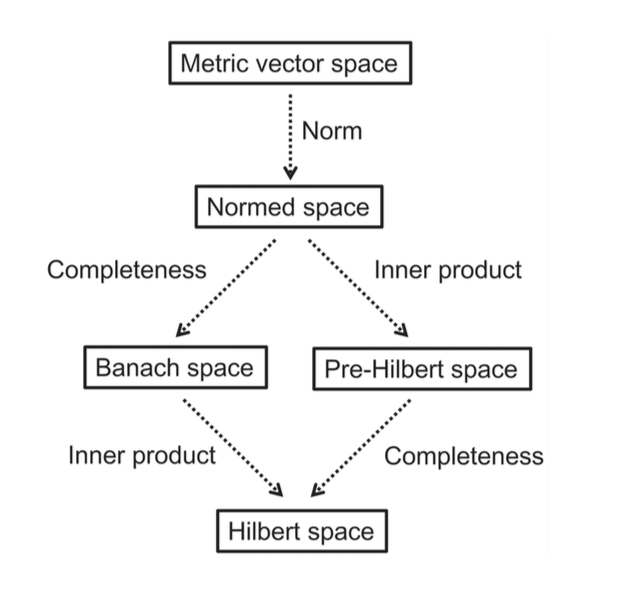
\includegraphics[width=8.58in]{images/math_Hilbertspacemap} 

}

\caption{Metric vector space로부터 힐버트 공간까지의 관계.}\label{fig:unnamed-chunk-31}
\end{figure}

벡터 공간(유한이어도 되고 무한이어도 된다)이 주어졌을 때, 벡터의 직교정규 집합은 만약 이것이 \textbf{완비(complete)}일 때에만 기저로서 작동한다. 만약 한 번 기저를 얻는다면, 그 공간의 벡터는 직교정규 벡터들의 선형 결합으로 분해할 수 있다. 그러나 무한히 많은 직교정규 기저로부터의 무한차원 공간에서 기저를 만들고자 할 때 한 가지 주의해야 할 점은 벡터들의 집합이 완비성을 만족하는지 체크해야 한다는 것이다. 이 주의점은 어떤 공간의 벡터들의 무한 합이 수렴하더라도, 그 극한이 같은 벡터 공간 안에 포함되지 않을 수 있다는 사실로부터 야기된다. 즉 이 극한은원래 공간으로부터 빗나가게 할 수 있게 한다. 이런 경우에는 벡터들의 집합이 무한차원 공간의 기저로써 더이상 작동하지 않는 것을 의미한다.

이러한 점을 좀 더 자세히 살펴보기 위해, 힐버트 공간 \(V\)에서의 직교정규 벡터들의 무한집합 \(\{ e_{i}\}\)에 대해 생각해보자. 그 다음에 우리는 한 개의 벡터 \(\mathbf{x}\in V\)를 골라 \(e_{i}\)의 내적을 계산한다. 그러면 \(\mathbf{x}\) 는 다음과 같이 표현된다.
\[c_{i}\langle e_{i},\mathbf{x} \rangle \in \mathbb{C}.\]
무한 수열 \(\{c_{i}\}\)와 \(\{e_{i}\}\)의 처음 \(n\)항을 사용해 우리는 다음과 같이 유한합
\[\sum_{i=1}^{n}c_{i}e_{i} \equiv \mathbf{x}_{n}\]
을 정의할 수 있다.

힐버트 공간의 대표적인 예로, \(L^{p}\) 공간이 있다.

\[\| f\|_{p}=(\int_{S}|f|^{p}d\mu)^{1/p}<\infty\]

박창이 교수님 외 책에서, 통계학에서 힐버트 공간을 고려하는 이유를 설명하였는데, 그 이유는 유한차원에서 성립하는 선형대수를 적용할 수 있기 때문이라고 한다. 특히 힐버트 공간은 완비(complete)된 공간으로써 알고리즘의 수렴성을 보장하며, 내적이 존재하므로써 직교성이나 정사영(projection)을 구할 수도 있다.

\hypertarget{holder-holder-space}{%
\subsection{Holder 공간(Holder space)}\label{holder-holder-space}}

이 공간의 정의는 \citep{Wasserman2006}를 참고하였다. 어떤 정수 \(m\)과 \(\delta \in (0,1)\)에 대해 \(s=m+\delta\)을 정의하자. \textbf{Holder 공간(Holder space)}(정확하게는 H"\{o\}lder space)은 bounded m차 derivative를 갖는, 즉 모든 \(u,t\)에 대해 \(|f^{m}(u)-f^{m}(t)|\leq |u-t|^{\delta}\)인 bounded function들의 집합니다.

\hypertarget{sobolev-sobolev-space}{%
\subsection{Sobolev 공간(Sobolev space)}\label{sobolev-sobolev-space}}

해석학에서 소볼레프 공간(Sobolev space)이란 충분히 매끄럽고, 무한대에서 충분히 빨리 0으로 수렴하는 함수들로 구성된 함수공간으로 르베그 공간의 일반화이다. 이 공간의 정의는 \citep{Wasserman2006}를 참고하였다. 이 책에서 Sobolev 공간의 정의는 smooth function들의 집합이라는 것이다. \(D^{j}f\)를 \(f\)의 \(j\)번째 weak derivative라고 하자. 먼저 weak differentiability에 대해 알아보자. \(f\)가 모든 bounded interval에서 적분 가능하다고 하자. 만약 다음꽈 같은 함수 \(f'\)가 존재해 모든 bounded interval에서 적분 가능하다면, 즉 모든 \(x\leq y\)에 대해
\[\int_{x}^{y}f'(s)ds=f(y)-f(x)\]
이라면 이를 \textbf{weakly differentiable}이라 부른다.

\BeginKnitrBlock{definition}[Sobolev 공간]
\protect\hypertarget{def:unnamed-chunk-32}{}{\label{def:unnamed-chunk-32} \iffalse (Sobolev 공간) \fi{} }\textbf{m차 Sobolev space}는 다음과 같다.
\[W(m)=\{ f \in L^{2}(0,1): D^{m}f \in L^{2}(0,1)\}\]

반지를 \(c\)를 갖는 \(m\)차 Sobolev space는 다음과 같다.
\[W(m,c)=\{ f \in W(m), \| D^{m}f \|^{2} \leq c^{2}\}\]

\textbf{주기를 갖는 Sobolev class (periodic Sobolev class)}는 다음과 같다.
\[\tilde{W}(m,c)=\{ f \in W(m,c): D^{j}f(0)=D^{j}f(1), j=0,\ldots, m-1 \}.\]
\EndKnitrBlock{definition}

\hypertarget{besov-besov-space}{%
\subsection{Besov 공간(Besov space)}\label{besov-besov-space}}

이 공간의 정의 또한 \citep{Wasserman2006}의 9장을 참고하였다. Wavelet threshold estimator는 Besov space에서 good optimality property를 갖는다. 다음과 같이 \(\Delta_{h}^{(r)}f(x)\)를 정의하자.
\[\Delta_{h}^{(r)}f(x)=\sum_{k=0}^{r}\binom{r}{k}(-1)^{k}f(x+kh).\]
그러면 \(\Delta_{h}^{(0)}f(x)=f(x)\)이고
\[\Delta_{h}^{(r)}f(x)=\Delta_{h}^{(r-1)}f(x+h)-\Delta_{h}^{(r-1)}f(x).\]
이다. 이제 \(w_{r,p}(f;t)\)를 다음과 같이 정의하자.
\[w_{r,p}(f;t)=\sup_{|h|\leq t}\|\Delta_{h}^{(r)}f\|_{p}.\]
이 때 \(\|g\|_{p}=\{ \int |g(x)|^{p}dx \}^{1/p}\)이다. \((p,g,\zeta)\)가 주어졌을 때, \(r\)이 존재해 \(r-1\leq \zeta \leq r\)을 만족한다면, \textbf{Besov seminorm} \(|f|_{p,q}^{\zeta}\)는
\[|f|_{p,q}^{\zeta}=[\int_{0}^{\infty}(h^{-\zeta}w_{r,p}(f;h))^{q}\frac{dh}{h}]^{1/q}\]
로 정의된다. \(q=\infty\)일 때는 다음과 같이 정의한다.
\[|f|_{p,\infty}^{\zeta}=\sup_{0<h<1}\frac{w_{r,p}(f;h)}{h^{\zeta}}\]

\BeginKnitrBlock{definition}[Besov 공간]
\protect\hypertarget{def:unnamed-chunk-33}{}{\label{def:unnamed-chunk-33} \iffalse (Besov 공간) \fi{} }\textbf{Besov 공간(Besov space)} \(B_{p,q}^{\xi}(c)\)는 \([0,1]\)에서 \(\mathbb{R}\)로 가는 함수 \(f\)들 중 \(\int |f|^{p}<\infty\)이고 \(|f|_{p,q}^{\zeta}\leq c\)인 \(f\)들의 집합니다.
\EndKnitrBlock{definition}

Sobolev space \(W(m)\)은 Besov ball \(B_{2,2}^{m}\)에 대응된다. Generalized Sobolev space \(W_{p}(m)\)은 \(m\)차 미분에서 \(L^{p}\) 노름을 사용하는 데 이것은 거의 Besov space와 비슷하다. 사실 \(B_{p,1}^{m} \subset W_{p}(m) \subset B_{p,\infty}^{m}\)이다. H"\{o\}lder space는 \(B_{\infty,\infty}^{m+\delta}\)와 같다. \(T\)를 bounded variation을 갖는 함수들을 포함하는 집합이라고 할 때, \(B_{1,1}^{1}\subset T \subset B_{1,\infty}^{1}\)을 만족한다. 즉 Besov space는 넓은 범위희 함수 공간들을 포함한다. 이에 수렴하는 수열(convergent sequence)와 코시 수열(Cauchy sequence)에 대해 생각해 볼 수 있다.

\hypertarget{skorohod-skorohod-space}{%
\subsection{Skorohod 공간(Skorohod space)}\label{skorohod-skorohod-space}}

\(D[a,b]\)을 right continuous하고 left limit을 갖는 함수들 \(z:[a,b]\rightarrow \mathbb{R}\)의 집합을 \textbf{Skorohod 공간(Skorohod space)}이라고 한다. \citep{VanderVaart2000} 257쪽에 나와있다.

\hypertarget{-expansion---besov-besov-spaces-in-terms-of-the-coefficients-of-the-wavelet-expansion}{%
\subsection{웨이블릿 expansion의 계수들로 이해하는 Besov 공간(Besov spaces in terms of the coefficients of the wavelet expansion)}\label{-expansion---besov-besov-spaces-in-terms-of-the-coefficients-of-the-wavelet-expansion}}

\hypertarget{---reproducing-kernel-hilbert-space}{%
\subsection{재생 커널 힐버트 공간(reproducing kernel Hilbert space)}\label{---reproducing-kernel-hilbert-space}}

재생 커널 힐버트 공간(reproducing kernel Hilbert space)이 주어지면 이에 대응되는 유일한 재생 커널이 존재한다. 역으로, 양정치 커널 \(K\)가 주어지면 \(K\)를 재생 커널로 갖는 유일한 재생 커널 힐버트 공간 \(\mathcal{H}\)가 존재한다.

\hypertarget{c--d-the-spaces-c-and-d}{%
\subsection{C 공간과 D 공간(the spaces C and D)}\label{c--d-the-spaces-c-and-d}}

\citep{Beran2013}의 appendix 참고

\hypertarget{-distance-and-metric}{%
\section{거리와 계량(distance and metric)}\label{-distance-and-metric}}

\hypertarget{distance}{%
\subsection{거리(distance)}\label{distance}}

\BeginKnitrBlock{definition}[거리]
\protect\hypertarget{def:unnamed-chunk-34}{}{\label{def:unnamed-chunk-34} \iffalse (거리) \fi{} }집합 \(X\)의 두 원소들 \(x,y\)에 대해 값 \(d(x,y)\)를 할당하는 함수 \(d(\cdot, \cdot)\)가 다음 세 조건들을

\begin{enumerate}
\def\labelenumi{\arabic{enumi}.}
\item
  임의의 \(x,y\in X\)에 대해서 \(d(x,y)\geq 0\)이다. 여기서 \(d(x,y)=0\)이기 위한 필요충분조건은 \(x=y\)이다.
\item
  임의의 \(x,y\in X\)에 대해서 \(d(x,y)=d(y,x)\)이다.
\item
  임의의 \(x,y,z\in X\)에 대해서 \(d(x,z)\leq d(x,y)+d(y,z)\)가 성립한다.
\end{enumerate}
\EndKnitrBlock{definition}

만약 \(d(\mathbf{x},\mathbf{y})=\| \mathbf{x}-\mathbf{y}\|\)라 하면 노름공간이 거리공간이 된다. 그러나 모든 거리공간이 노름공간으로부터 유도되는 것은 이니다.

군집분석 방법에서는 관측값들의 거리를 이용해 군집을 나눌 때 사용된다.

\begin{itemize}
\item
  유클리드 거리(Euclidean distance): \(d(x,y)=(\sum_{i=1}^{p}(x_{i}-y_{i})^{2})^{1/2}\)
\item
  민콥스키 거리(Minkowski distance): \(d(x,y)=(\sum_{i=1}^{p}(x_{i}-y_{i})^{m})^{1/m}\)
\item
  맨하탄 거리(Manhattan distance): \(d(x,y)=\sum_{i=1}^{p}|x_{i}-y_{i}|\)
\item
  표준화 거리(standardized distance): \(d(x,y)=(\sum_{i=1}^{p}(x_{i}-y_{i})^{2}/s_{i}^{2})^{1/2}\), 여기서 \(s_{i}\)는 \(i\)번째 변수에 대한 표준편차
\item
  마할라노비스 거리(Mahalanobis distance): \(d(x,y)=(x-y)^{T}\boldsymbol{\Sigma}^{-1}(x-y)\), 여기서 \(\Sigma\)는 공분산행렬
\item
  체비셰프 거리(Chebychev distance): \(d(x,y)=\max_{i=1,\ldots ,p}|x_{i}-y_{i}|\)
\end{itemize}

다음 거리들은 유클리드 거리와 더불어 공간통계에서 많이 쓰이는 것들이다.

\begin{itemize}
\item
  chordal distance (현 거리? 잘 모르겠음)
\item
  geodesic distance
\end{itemize}

다른 거리들도 있다.

\begin{itemize}
\tightlist
\item
  Hamming distance: \citep{Massart2007} 책에 나오는 것으로 \(\mathcal{X}^{n}\)을 \(n\)개의 확률변수들이 값을 취하는 \(n\)차원 공간이라고 할 때 다음과 같다.
  \[d(y,y')=\sum_{i=1}^{n}\mathbb{I}_{y_{i}\neq y'_{i}}, \qquad{\forall y,y'\in\mathcal{X}^{n}}\]
\end{itemize}

\hypertarget{metric}{%
\subsection{계량(metric)}\label{metric}}

계량(metric)은 두 집합 사이의 모든 원소 짝의 거리를 지정해주는 함수이다.

\hypertarget{-sequences-of-real-functions}{%
\section{실함수의 수열들(sequences of real functions)}\label{-sequences-of-real-functions}}

이 부분의 내용은 \citep{Polansky2011}의 내용을 따른다.

확률변수(random variable)의 수열이 함수의 수열처럼 여겨질 수 있다는 사실에서 함수의 수열의 성질을 이해하는 것은 중요하다. 일반적인 수열의 수렴에 관한 성질들과 비교했을 때 함수의 수열들의 수렴에 관한 성질에서는 여러 개의 정의로 다뤄질 수 있다는 점에서 차이가 있다. 가장 널리 알려진 함수의 수렴은 \textbf{점별수렴(pointwise convergence)}과 \textbf{균등수렴(uniform convergence)}이 있다.

\BeginKnitrBlock{definition}[점별수렴]
\protect\hypertarget{def:unnamed-chunk-35}{}{\label{def:unnamed-chunk-35} \iffalse (점별수렴) \fi{} }\(\{ f_{n}(x)\}_{n=1}^{\infty}\)를 실함수의 수열이라고 하자. 그러면 모든 \(x\in\mathbb{R}\)에 대해
\[\lim_{n\rightarrow \infty}f_{n}(x)=f(x)\]
를 만족하는 실함수 \(f\)가 존재할 때 수열 \(\{ f_{n}(x)\}_{n=1}^{\infty}\)이 \(f\)에 \textbf{점별수렴(pointwise convergence)}한다고 한다. 여기서는 \(n\rightarrow \infty\)일 때
\[f_{n} \stackrel{pw}{\rightarrow} f\]
로 표현하기로 한다.
\EndKnitrBlock{definition}

점별수렴에서 수렴 문제는 \(x\)를 고정된 실수로 놓았을 때 실수열 \(\{f_{n}(x)\}_{n=1}^{\infty}\)의 수렴 성질을 보는 것으로 줄일 수 있다.

다음은 \citep{Shima2016}에 나오는 점별수렴하는 함수열의 예제다.

\BeginKnitrBlock{definition}[점별수렴의 예]
\protect\hypertarget{def:unnamed-chunk-36}{}{\label{def:unnamed-chunk-36} \iffalse (점별수렴의 예) \fi{} }다음과 같은 닫힌 구간 \([0,1]\)에서 정의된 함수열 \(\{f_{n}\}\)
\[f_{n}(x)=x^{n}\]
이 있다고 하자. 이 수열은 다음 함수로 점별수렴한다.
\[
f(x)=\lim_{n\rightarrow\infty}f_{n}(x)=
\begin{cases}
0 & 0\leq x < 1\\
1 & x=1.
\end{cases}
\]
\EndKnitrBlock{definition}

\begin{figure}

{\centering 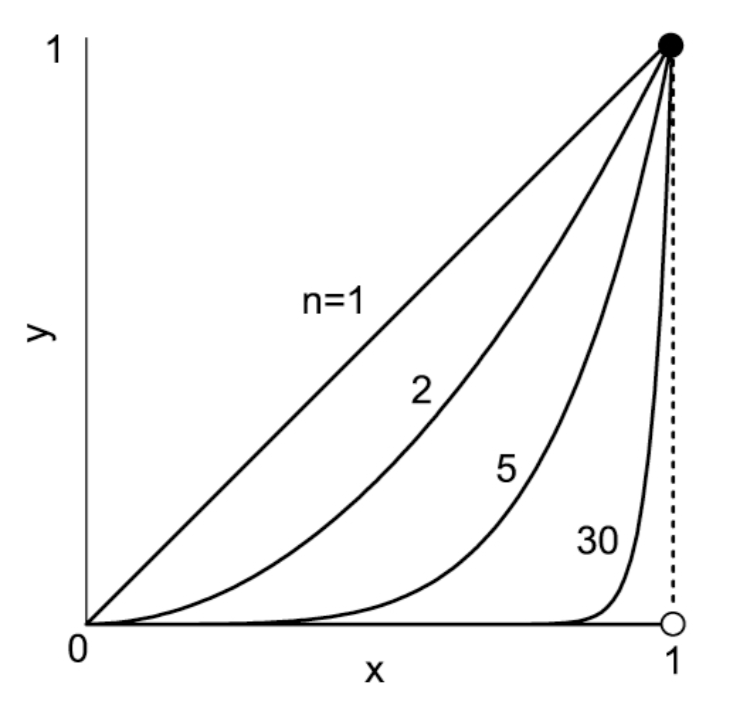
\includegraphics[width=10.33in]{images/math_ptconvergence} 

}

\caption{점별수렴하는 함수의 예.}\label{fig:unnamed-chunk-37}
\end{figure}

또한 \citep{Shima2016}에서 언급한 내용 중 중요한 사실은 점별수렴의 경우에는 앞의 예제에서처럼 원래 함수열들이 모두 연속이라 할지라도 그것의 극한 함수는 연속이 아닐 수도 있다는 점이다. 위 예제에서 \(f(x)\)는 \(x=1\)에서 불연속이다(그림). 이 말은 또한 점별수렴에서는 극한의 순서를 바꾸었을 경우 그 결과가 아래 식처럼 서로 다를 수 있음을 의미한다.
\[\lim_{x\rightarrow 1}\lim_{n\rightarrow\infty}f_{n}(x)\neq \lim_{n\rightarrow\infty}\lim_{x\rightarrow 1}f_{n}(x).\]

이런 현상은 함수열 \(f_{n}(x)\)의 미분가능성과 적분가능성에서도 비슷하게 일어난다. 즉, 점별수렴 하에서는 함수열들이 모두 적분가능하거나 미분가넝하더라고 그것의 극한은 그렇지 않을 수도 있음을 의미한다. 이러한 예제들로 다음 예제들이 있다.

\BeginKnitrBlock{definition}[점별수렴과 적분의 순서]
\protect\hypertarget{def:unnamed-chunk-38}{}{\label{def:unnamed-chunk-38} \iffalse (점별수렴과 적분의 순서) \fi{} }다음과 같은 함수
\[f_{n}(x)=nx(1-x^{2})^{n}, \qquad{x\in [0,1]}\]
이 있다고 하자. 여기서는 극한과정 \(n\rightarrow\infty\)와 적분의 순서를 바꾸면 다른 결과를 줄 것임을 보여줄 것이다. 주어진 함수는 각각의 \(n\)에 대해 적분 가능하며 다음과 같다.
\[
\begin{align*}
\int_{0}^{1}f_{n}(x)dx &= n \int_{0}^{1}x(1-x^{2})^{n}dx = \Big[\frac{-n}{2(n+1)}(1-x^{2})^{n+1}\Big]_{0}^{1}\\
&= \frac{n}{2(n+1)}\rightarrow \frac{1}{2}.
\end{align*}
\]

반대로, 극한은 다음과 같다.
\[f(x)=\lim_{n\rightarrow\infty}f_{n}(x)=0, \qquad{\forall x\in [0,1].}\]

따라서 당연히 \(\int_{0}^{1}f(x)dx=0\)이다. 그래서 다음과 같은 결론을 내릴 수 있다.
\[\lim_{n\rightarrow\infty}\int_{0}^{1}f_{n}(x)dx\neq \int_{0}^{1}\lim_{n\rightarrow\infty}f_{n}(x)dx.\]

결론은, 점별수렴 과정에서는 극한 과정과 적분의 순서를 바꾸는 것은 안되다는 것이다.
\EndKnitrBlock{definition}

\BeginKnitrBlock{definition}[점별수렴과 미분의 순서]
\protect\hypertarget{def:unnamed-chunk-39}{}{\label{def:unnamed-chunk-39} \iffalse (점별수렴과 미분의 순서) \fi{} }다음과 같은 함수
\[
f_{n}(x)=
\begin{cases}
-1 & x < -\frac{1}{n},\\
\sin(\frac{n\pi x}{2}) & -\frac{1}{n} < x \frac{1}{n},\\
1 & x>\frac{1}{n}.
\end{cases}
\]
우리는 이 함수의 \(x=0\)에서의 극한 \(f(x)=\lim_{n\rightarrow\infty}f_{n}(x)\)의 연속성을 점검해 볼 것이다. \(f_{n}(x)\)는 모든 \(x\in \mathbb{R}\)에서 미분 가능하므로 당연히 모든 \(n\)에서 \(x=0\)일 때 연속이다. 그러나 그것의 극한은
\[
f(x)=
\begin{cases}
-1 & x<0,\\
0 & x=0, \\
1 & x >0
\end{cases}
\]
이며 \(x=0\)에서 불연속이다. 따라서 점별수렴 과정에서는 극한 과정과 미분의 순서를 바꾸는 것은 안된다.
\EndKnitrBlock{definition}

점별수렴보다 더 강한 조건으로 \(x \in \mathbb{R}\)에 상관 없이 모든 지점에서 동시에 \(n\rightarrow\infty\)일 때 \(f_{n}(x) \rightarrow f(x)\)이길 요구할 수도 있다. 이 때 사용되는 정의가 균등수렴이다.

\BeginKnitrBlock{definition}[균등수렴]
\protect\hypertarget{def:unnamed-chunk-40}{}{\label{def:unnamed-chunk-40} \iffalse (균등수렴) \fi{} }\(\{ f_{n}(x)\}_{n=1}^{\infty}\)를 실함수의 수열이라고 하자. 그러면 모든 \(\epsilon > 0\)에 대해
\[|f_{n}(x)-f(x)| <\epsilon \forall n \geq n_{\epsilon} \text{ and } x\in \mathbb{R}\]
을 만족시키는 정수 \(n_{\epsilon}\)이 존재할 때 수열 \(\{ f_{n}(x)\}_{n=1}^{\infty}\)이 \(f\)에 \textbf{균등수렴(uniform convergence)}한다고 한다. 여기서는 \(n\rightarrow \infty\)일 때
\[f_{n} \stackrel{u}{\rightarrow} f\]
로 표현하기로 한다.
\EndKnitrBlock{definition}

\begin{figure}

{\centering 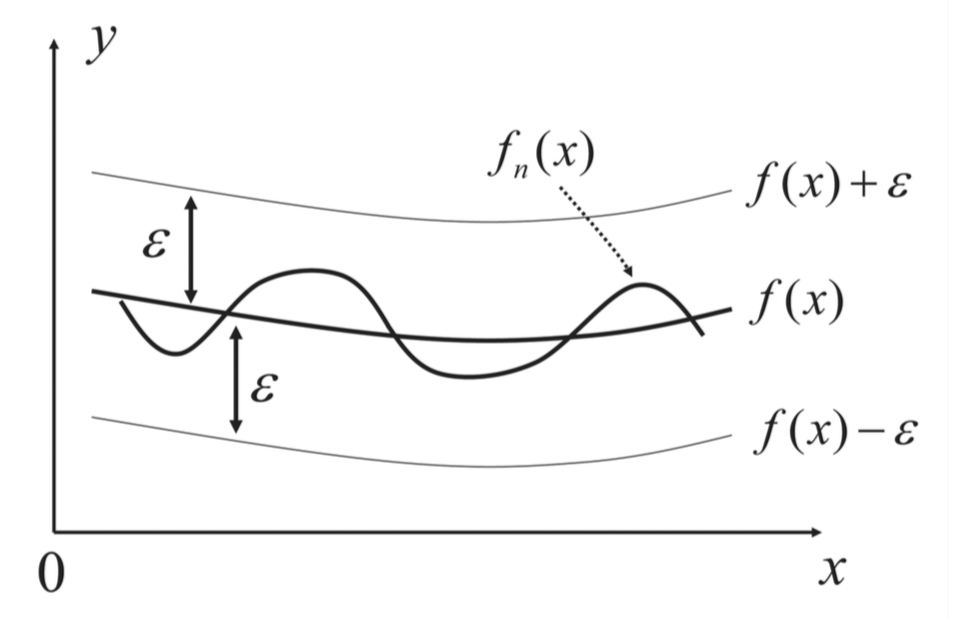
\includegraphics[width=13.28in]{images/math_uniformconvergence} 

}

\caption{균등수렴하는 함수의 예. 균등수렴에서는 어떤 밴드를 잡았을 때, n을 적당히 조절하여 함수열이 그 밴드 안에 들어가도록 할 수 있다.}\label{fig:unnamed-chunk-41}
\end{figure}

균등수렴과 관련된 정리로 어떤 연속함수들의 함수열이 균등수렴이면 그 수열의 극한 또한 반드시 연속이어야 한다는 정리가 있다. 이 정리는 \citep{Polansky2011}에 나와있다.

\BeginKnitrBlock{theorem}[함수열의 균등수렴과 함수열의 극한의 연속]
\protect\hypertarget{thm:unnamed-chunk-42}{}{\label{thm:unnamed-chunk-42} \iffalse (함수열의 균등수렴과 함수열의 극한의 연속) \fi{} }\(\{f_{n}(x)\}_{n=1}^{\infty}\)가 \(\mathbb{R}\)의 부분집합 \(R\)에서 정의된 함수들의 수열이며 함수 \(f\)로 균등수렴한다고 하자. 만약 각각의 \(f_{n}\)들이 어떤 점 \(x\in R\)에서 연속이면, \(f\) 또한 점 \(x\)에서 연속이어야 한다.
\EndKnitrBlock{theorem}

이 정리의 증명은 Apostol (1974)의 9.4절에서 발견할 수 있다고 한다. 여기서 알아두어야 할 것은 균등수렴은 충분조건이며 필요조건이 아니라는 것이다. 즉

\hypertarget{-convergent-sequence}{%
\subsection{수렴하는 수열(convergent sequence)}\label{-convergent-sequence}}

\BeginKnitrBlock{definition}[(함수해석학에서) 수렴하는 수열]
\protect\hypertarget{def:unnamed-chunk-43}{}{\label{def:unnamed-chunk-43} \iffalse ((함수해석학에서) 수렴하는 수열) \fi{} }노름 벡터 공간 \((\mathcal{F}, \| \cdot\|_{\mathcal{F}})\)의 원소들로 이루어진 수열 \(\{ f_{n}\}_{n=1}^{\infty}\)가 모든 \(\epsilon >0\)에 대해 \(N=N(\epsilon)\in \mathbb{N}\)이 존재해 모든 \(n \geq \mathbb{N}\)에 대해 \(\| f_{n}-f\|_{\mathcal{F}} <\epsilon\)을 만족할 때, 우리는 수열이 \(f\in \mathcal{F}\)에 \textbf{수렴(converge)} 한다고 한다.
\EndKnitrBlock{definition}

\hypertarget{-cauchy-sequence}{%
\subsection{코시 수열(Cauchy sequence)}\label{-cauchy-sequence}}

\BeginKnitrBlock{definition}[(함수해석학에서) 수렴하는 수열]
\protect\hypertarget{def:unnamed-chunk-44}{}{\label{def:unnamed-chunk-44} \iffalse ((함수해석학에서) 수렴하는 수열) \fi{} }노름 벡터 공간 \((\mathcal{F}, \| \cdot\|_{\mathcal{F}})\)의 원소들로 이루어진 수열 \(\{ f_{n}\}_{n=1}^{\infty}\)가 모든 \(\epsilon >0\)에 대해 \(N=N(\epsilon)\in \mathbb{N}\)이 존재해 모든 \(m,n \geq \mathbb{N}\)에 대해 \(\| f_{m}-f_{n}\|_{\mathcal{F}} <\epsilon\)을 만족할 때, 수열 \(\{ f_{n}\}_{n=1}^{\infty}\)를 \textbf{코시 수열(Cauchy sequence)}이라고 한다.
\EndKnitrBlock{definition}

\BeginKnitrBlock{example}[유리수의 장]
\protect\hypertarget{exm:unnamed-chunk-45}{}{\label{exm:unnamed-chunk-45} \iffalse (유리수의 장) \fi{} }절대값 \(\| \cdot\|\)을 노름으로 갖는 유리수 \(\mathbb{Q}\)의 장(field)은 노름 벡터 공간이다. 여기서 수열 \(1, 1.4, 1.41, \ldots\)는 \(\mathbb{Q}\)에서의 코시 수열이나 이것의 극한 \(\sqrt{2} \notin \mathbb{Q}\)이므로 수렴하는 수열은 아니다.
\EndKnitrBlock{example}

\BeginKnitrBlock{example}[C[0,1]]
\protect\hypertarget{exm:unnamed-chunk-46}{}{\label{exm:unnamed-chunk-46} \iffalse (C{[}0,1{]}) \fi{} }\(C[0,1]\)을 구간 \([0,1]\)에서 bounded continuous인 함수들의 집합이라고 하자. 다음과 같은 노름 \(\| f\| =(\int_{0}^{1}|f(x)|^{2}dx)^{1/2}\)을 생각할 때 함수들의 수열 \(\{ f_{n}\}\)은 \([0, \frac{1}{2}-\frac{1}{2n} ]\)에서 \(0\)이고 \([\frac{1}{2}+\frac{1}{2n}, 1]\)에서 \(1\)이기 때문에 코시 수열이나 연속 극한(continuous limit)은 존재하지 않는다.
\EndKnitrBlock{example}

\begin{figure}

{\centering 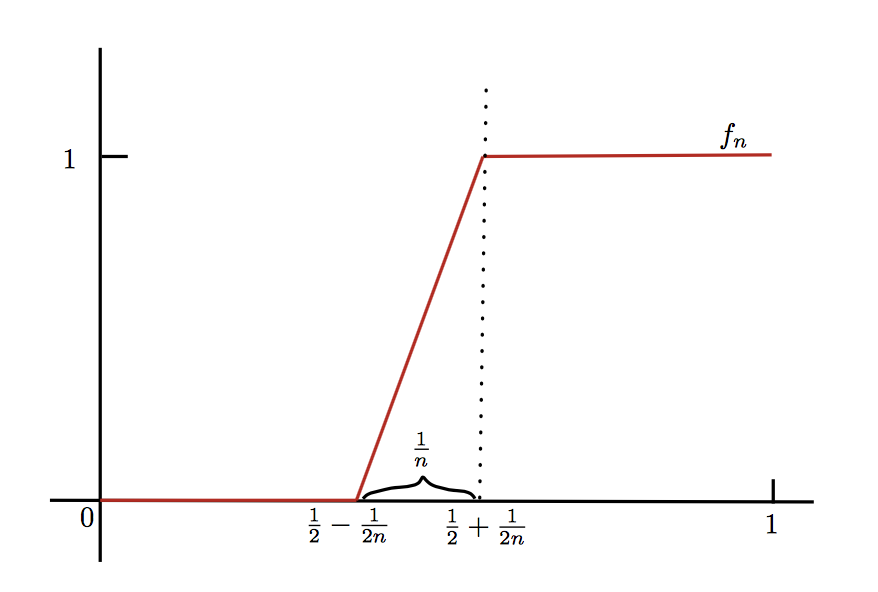
\includegraphics[width=12.19in]{images/math_counterCauchy} 

}

\caption{L2 norm에서 연속 극한을 갖지 않는 연속함수들의 코시 수열의 예.}\label{fig:unnamed-chunk-47}
\end{figure}

\hypertarget{continuity}{%
\section{연속(continuity)}\label{continuity}}

\hypertarget{-lipschitz-continous}{%
\subsection{립쉬츠 연속(Lipschitz continous)}\label{-lipschitz-continous}}

\citep{Abbott2015}의 문제 4.4.9를 참고하였다. 어떤 함수 \(f:A\rightarrow \mathbb{R}\)이 \textbf{립쉬츠 연속(Lipschitz continous)}이라는 것은 모든 \(x\neq y\)에 대해 유계 \(M >0\)이 존재해
\[|\frac{f(x)-f(y)}{x-y}|\leq M\]
을 만족하는 것이다. 기하학적으로 말하면 어떤 함수 \(f\)가 립쉬츠라는 것은 \(f\)의 임의의 두 점을 잡아 기울기를 계산해도 그것을 cover할 수 있는 uniform bound가 존재한다는 것이다. 만약 \(f\)가 미분 가능할 경우 \(x\)가 \(y\)랑 매우 가까워지게 되면 좌변은 미분의 절대값임을 알 수 있다. 그러나 립쉬츠 연속이 \(f\)가 미분가능함을 말하는 것은 아니다. 단지 \(f\)가 너무 가파르지 않은 함수라는 것만 알 수 있을 뿐이다.

\begin{itemize}
\tightlist
\item
  함수 \(f:A\rightarrow \mathbb{R}\)가 립쉬츠이면 그 함수는 또한 \(A\)에서 uniformly continuous하다.
\end{itemize}

\hypertarget{measure}{%
\chapter{측도}\label{measure}}

권순식 교수님의 르베그 적분론 강의노트를 참고하였다. Pivato의 Analysis, Measure, and Probability: A visual introduction 또한 참고하였다. \textbf{측도(measure)}란 수학에서, \textbf{양(quantity)}이라 개념을 반영하기 위해 만들어진 장치다.

\begin{figure}

{\centering 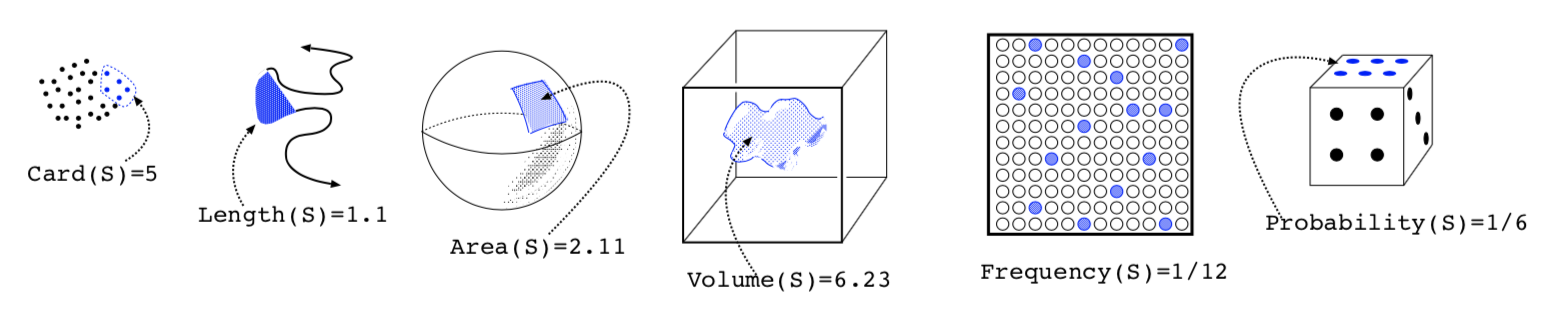
\includegraphics[width=21.78in]{images/math_measure_intro} 

}

\caption{Cardinality, length, area, volume, frequency and probability.}\label{fig:unnamed-chunk-48}
\end{figure}

\(\mathbf{X}\)를 집합이라고 하자. 그리고 부분집합들 \(\mathbf{U,V}\subset \mathbf{X}\)이 있는데 이들의 'size'를 비교하고 싶어한다. 이런 'quantity'의 개념들은 여러가지가 있다.

\begin{itemize}
\item
  \textbf{Cardinality}: 이산 집합에 해당하는 것으로 어떤 지역의 인구 수나 가방 안의 구슬들의 숫자 등이 해당된다.
\item
  \textbf{Length}: 줄과 같은 1차원 물체에 적용할 수 있다.
\item
  \textbf{Area}: 카펫과 같은 2차원 물체에 적용할 수 있다.
\item
  \textbf{Volume}: 물병의 용량과 같은 3차원 물체에 적용할 수 있다.
\item
  \textbf{Mass}: 물질의 양을 잴 때 사용한다.
\item
  \textbf{Charge}: 전자기기에 사용된는 양의 크기
\item
  \textbf{Average Frequency}: 종종 어떤 사건이 일어날 때 평균의 양을 정하기 위해 사용한다. 이러한 주기들은 가법성을 갖는다. 예를 들면 1년 중 흐린 날의 숫자를 센다고 했을 때 이들은 흐리면서 비온날 + 흐리면서 비는 안온날 의 합으로 생각할 수 있다.
\item
  \textbf{Probability}: 어떤 사건이 일어날 것의 승산(odds)을 말하며 이들 또한 가법성을 갖는다.
\end{itemize}

\hypertarget{--limitation-of-riemman-integral}{%
\section{리만 적분의 한계정(limitation of Riemman integral)}\label{--limitation-of-riemman-integral}}

전형적인 적분(integral) \(\int_{A}f(x)dx\)는 다음으로 구성되어있다.

\begin{itemize}
\item
  \(A\): the set of integration (or the domain of integration)
\item
  \(f(x)\): the integrand
\item
  \(dx\): the integrator
\end{itemize}

다시 말해서, 적분이란 것은 연속적으로 변하는 물체들의 합인 것이다. 이는 역사적으로 적분기호 \(\int\)가 합을 뜻하는 sum의 \(S\)에서 온 것에서도 확인할 수 있다. 이 적분은 다음
\[\sum_{\alpha\in I}\max_{x\in A_{\alpha}}f(x)|A_{\alpha}| \text{ or } \sum_{\alpha\in I}\min_{x\in A_{\alpha}}f(x)|A_{\alpha}|\]
을 근사한다. 이 때 우리는 적분을 하고자 하는 집합 \(A\)를 disjoint set으로 나눌 수 있다, 즉 \(A=\bigcup_{\alpha\in I}A_{\alpha}\)로 나눌 수 있다고 가정하고 각 집합 \(A_{\alpha}\) 에서 \(f\)는 거의 상수라고 가정한다. 여기서 우리는 \(|A_{\alpha}|\)를 집합 \(A_{\alpha}\)의 size라고 하자. 그리고 \(\max_{x\in A_{\alpha}}f(x)\) 또는 \(\min_{x\in A_{\alpha}}f(x)\)를 \(A_{\alpha}\)에서의 함수값들을 대표하는 값으로 선택된 것이라 생각해보자. 가장 쉽게 질문할 수 있는 것은 `어떻게 set의 size를 정할 것인가?' 라는 문제가 있다.

\textbf{리만 적분(Riemman integral)}에서는 interval (또는 rectangle, cube 등등)들의 size만 측도(measure)하면 된다.

\BeginKnitrBlock{example}[정의역과 치역이 1차원인 함수에서의 리만 적분]
\protect\hypertarget{exm:unnamed-chunk-49}{}{\label{exm:unnamed-chunk-49} \iffalse (정의역과 치역이 1차원인 함수에서의 리만 적분) \fi{} }\(f\)를 \(\mathbb{R}\)에서 정의된 함수고 정의역이 \([a,b]\)라고 하자. 그러면 우리는 구간 \([a,b]\)를 더 잘게, \([x_{0}=a,x_{1}], [x_{1},x_{2}],\ldots, [x_{n-1},x_{n}=b]\)로 나누고 적분을 다음 값으로 근사한다.
\[\sum_{i=1}^{n}f(x_{i})|x_{i}-x_{i-1}|.\]
이 합의 극합이 적분값이 되며 우리는 이 적분을 리만 적분이라고 부른다. 여기서는 \(\mathbb{R}\)에서의 집합들의 크기(size)를 측도하기 위해 interval을 사용하였다.
\EndKnitrBlock{example}

\begin{figure}

{\centering 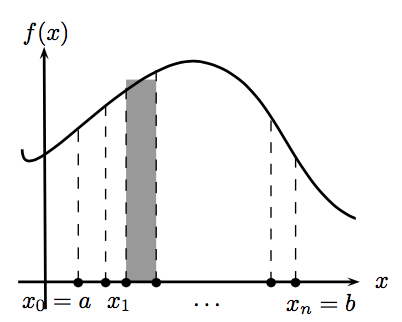
\includegraphics[width=5.58in]{images/math_measure_Riemann1d} 

}

\caption{1차원 공간의 정의역을 자르는 방법.}\label{fig:unnamed-chunk-50}
\end{figure}

\begin{figure}

{\centering 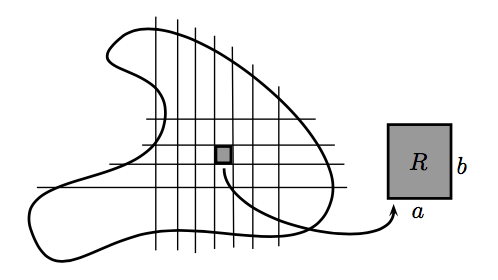
\includegraphics[width=6.92in]{images/math_measure_Riemann2d} 

}

\caption{2차원 공간의 정의역을 자르는 방법. 이 경우에는 사각형의 면적이 집합의 크기가 된다.}\label{fig:unnamed-chunk-51}
\end{figure}

그러나, 불연속 함수의 경우에는 interval (또는 rectangle, cube 등등)의 크기를 재는 것이 적분을 정의하기에 충분치 않을 수도 있다. 따라서 우리는 먼저 집합의 크기를 정의하는 것 부터 다시 정의할 필요가 있다. 이제부터 '집합의 크기(size)'를 집합의 \textbf{측도(measure)}라고 부를 것이다. \textbf{측도함수(measure function)} \(m\)는
\[m:\mathcal{M}\rightarrow [0,\infty], \mathcal{M}\subseteq\mathcal{P}(\mathbb{R}^{n})\]
이다. 즉 \(\mathcal{M}\)dms \(\mathcal{P}(\mathbb{R}^{n})\)의 subcollection이다. 이제 여기서의 목표는 적분이론에 잘 맞는 적절한 \(m,\mathcal{M}\)을 찾는 것이다. 그런데 우리가 모든 \(\mathcal{P}(\mathbb{R}^{n})\)에 대해 \(m\)을 정의할 수 있을까? 만약 그렇지 않다면, 적어도 우리는 \(\mathcal{M}\)에서의 측도 \(m\)이 interval이나 rectangle, open set, compact set 등 좋은 '집합'들에서 모두 잘 정의되게끔 구성하고자 한다. 더 나아가, 우리는 이 적분함수 \(m\)을 우리 직관에 일치하도록 확장시키고자 한다. 그 직관이란,

\begin{itemize}
\item
  \(m(\emptyset)=0\)
\item
  \(m([a,b])=b-a\) 또는 \(m(\text{Rectangle})=|\text{vertical side}|\times |\text{horizontal side}|\)
\item
  만약 \(A\subset B\)인 경우 \(m(A)\leq m(B)\)
\item
  만약 \(A,B\)가 disjoint인 경우 \(m(A\cup B)=m(A)+m(B)\)
\item
  더 나아가, 우리는 측도가 countable additivity를 갖길 원한다. 즉 \(A_{i},i=1,2,\ldots\)가 disjoint이면 \(\sum_{i=1}^{m}=m(\cup_{i=1}^{\infty}A_{i}).\)
\end{itemize}

정리하면, 만족스러운 적분이론을 얻기 위해 우리는 \(\mathbb{R}^{n}\)에서의 충분히 큰 subset들의 class에 대해 잘 정의되는 측도를 구성하고자 한다. 그러면 여기서 리만 적분으로는 불충분한 점들을 몇 가지 짚고 넘어가고자 한다.

우선, 리만 적분이 가능하려면, `대부분의' 작은 interval에서 \(\max f - \min f\)가 매우 작아야한다. 즉, 리만 적분 가능성은 함수의 연속성과 관련이 있다. 실제로 함수 \(f\)가 리만 적분 가능하려면 \(f\)가 거의 모든 지점에서 연속이어야 한다(이는 필요충분조건이다).

\BeginKnitrBlock{example}[리만 적분이 안되는 함수]
\protect\hypertarget{exm:unnamed-chunk-52}{}{\label{exm:unnamed-chunk-52} \iffalse (리만 적분이 안되는 함수) \fi{} }다음과 같이 함수 \(f_{\text{Dir}}(x)\)를 정의하자
\[
f_{\text{Dir}}(x) = 
\begin{cases}
1 & \text{if $x\in\mathbb{Q}$} \\
0 & \text{if $x\in\mathbb{Q}^{c}$.}\\
\end{cases}
\]

그리면 임의의 구간 \(I\subset\mathbb{R}\)에 대해
\[\max_{x\in I}f_{\text{Dir}}(x) =1 \text{ and } \min_{x\in I}f_{\text{Dir}}(x) =0\]
이므로 \(f_{\text{Dir}}(x)\)는 리만적분이 가능하지 않다. 참고로 함수 \(f_{\text{Dir}}(x)\)는 어디에서도 연속이 아니다.
\EndKnitrBlock{example}

두 번째로, 리만 적분 이론에서는 적분의 정의역(domain)을 분해하기 위해 오로지 interval, rectangle 또는 cube 등등만을 고려한다. 그래서 우리는 interval을 어떻게 측도해야할지 알아야 한다. 그러나 어떤 함수드에서는, 다른 형태로 정의역을 분해하는 것이 좀 더 자연스러울 때가 있다. 예를 들면, 우리가 \(\mathbb{Q}\) 또는 \(\mathbb{Q}^{c}\)에서의 측도를 정의하고자 할 때, 가장 자연스럽게 생각할 수 있는 것으로는 다음과 같은 적분이 있다.
\[\int_{0}^{1}f_{\text{Dir}}(x)dx:=1\cdot |\mathbb{Q}\cap [0,1]| + 0\cdot |\mathbb{Q}^{c}\cap [0,1]|.\]

마지막으로, 우리가 다음과 같은 함수들의 수열 \(\{f_{n}:[0,1]\rightarrow\mathbb{R} \}\)을 정의했을 때,
\[
f_{n}(x) := 
\begin{cases}
1 & \text{if $x=p/q$ where $p,q\in\mathbb{Z}$ and $q\leq n$} \\
0 & \text{otherwise.}\\
\end{cases}
\]

\(f_{n}\)들은 유한히 많은 점들을 제외하고 모두 연속이므로 리만 적분가능하다. 더불어 \(n\rightarrow \infty\)일 때 \(f_{n}\rightarrow f_{\text{Dir}}\)이다. 그러나 앞서 살펴본대로 \(f_{\text{Dir}}\)은 리만 적분 가능하지 않다. 이 예는 모든 함수들의 수열이 리만 적분 가능하더라도, 그것의 극한은 리만 적분 가능하지 않을 수도 있다는 것을 보여준다. 단 \(\{f_{n}\}\)이 \(f\)로 uniform converge 하는 경우에는 \(f\)는 항상 리만 적분 가능하다.

\hypertarget{outer-measure}{%
\section{외측도(outer measure)}\label{outer-measure}}

외측도 부분은 Christopher E. Heil의 real analysis 강의 2.5를 참고하였다. 보통의 경우에는 우리가 어떻게 측도를 만들 수 있는지 아는 \(\mathbb{R}^{d}\)의 부분집합의 basic class들(rectangular box 또는 cube)로부터 시작한다. 여기서는 그들의 부피로 측도를 정의할 수 있다. 그 다음에는 이 측도의 개념을 \(\mathbb{R}^{d}\)의 모든 부분집합들로 확장할 방법을 찾아야 한다. 모든 부분집합 \(E \subset \mathbb{R}^{d}\)에서 우리는 음이 아니고 확정된 실수값을 갖는 숫자를 정의할 수 있으며 cube의 개념을 확장한 개념으로 \textbf{exterior Lebesgue measure} \(\mu^{*}(E)\) 또는 \(|E_{e}|\)로 정의한다. 여기서 좋은 점은 \(\mathbb{R}^{d}\)의 모든 부분집합은 유일하게 정의된 exterior measure를 갖는다는 것이다. 그러나 문제점도 한 가지 있는데, \(\mu^{*}\)가 측도가 아니란 것이다.(이것은 countably subadditive이지만 not countably additive이다)

\BeginKnitrBlock{definition}[외측도]
\protect\hypertarget{def:unnamed-chunk-53}{}{\label{def:unnamed-chunk-53} \iffalse (외측도) \fi{} }\(X\)를 공집합이 아닌 집합이라고 하자. \(X\)에서의 \textbf{외측도(outer measure, or exterior measure)}는 함수 \(\mu^{*}:\mathcal{P}(X)\rightarrow [0,\infty]\)이며 다음의 조건들을 만족한다.

\begin{enumerate}
\def\labelenumi{\arabic{enumi}.}
\item
  \(\mu^{*}(\emptyset) = 0.\)
\item
  (monotinicity) 만약 \(A\subseteq B\)이면 \(\mu^{*}(A)\leq \mu^{*}(B)\)이다.
\item
  (countable subadditivity) 만약 \(E_{1},E_{2},\ldots \subseteq X\)이면 \(\mu^{*}(\bigcup_{k}E_{k})\leq \sum_{k}\mu^{*}(E_{k})\)이다.
\end{enumerate}
\EndKnitrBlock{definition}

외측도 \(\mu^{*}\)가 주어졌을 때, 우리의 목표는 \(X\)에서의 \(\sigma\)-체 \(\Sigma\)를 만들어 \(\Sigma\)에 제한된 \(\mu^{*}\)가 countably additive하게 만드는 것이다. \(\Sigma\)의 원소들은 좋은 집합들이 되어야 하는데, 이 좋은 집합들이란 \(\mu^{*}\)에 대해 가측인 것이다. 그렇다면 우리는 임의의 외측도에서 측도가능성을 어떻게 정의할 수 있을까? \(X\)의 위상이 주어지지 않을 가능성도 있어, 측도가능성을 주변을 둘러싼 열린 집합들로 정의할 수 없다.

\BeginKnitrBlock{definition}[가측집합]
\protect\hypertarget{def:unnamed-chunk-54}{}{\label{def:unnamed-chunk-54} \iffalse (가측집합) \fi{} }\(\mu^{*}\)가 집합 \(X\)에서의 외측도라고 하자. 그러면 어떤 집합 \(E\subseteq X\)는
\[\forall A\subseteq X, \mu^{*}(A)=\mu^{*}(A\cap E) + \mu^{*}(A\backslash E)\]
일 때 \(\mu^{*}\)-가측 또는 단순히 \textbf{가측(measurable)}이라고 부른다.
\EndKnitrBlock{definition}

\BeginKnitrBlock{remark}[외측도의 따름정리]
\iffalse{} {Remark (외측도의 따름정리). } \fi{}1. 공집합은 \(\mu^{*}(\emptyset)=0\)이라는 사실에 비롯하여 \(\mu^{*}\)-가측이다.

\begin{enumerate}
\def\labelenumi{\arabic{enumi}.}
\setcounter{enumi}{1}
\tightlist
\item
  Subadditivity (쉽게 얘기해서, \(A\)가 어떤 함수 \(f\)의 domain이라고 할 때 \(\forall x,y\in A, f(x+y)\leq f(x)+f(y)\)를 얘기함)에 의해 다음의 부등식이 성립한다.
  \[\mu^{*}(A) \leq \mu^{*}(A\cap E) + \mu^{*}(A\backslash E).\]
  따라서 어떤 \(E\)가 가측임을 보이려면 모든 집합 \(A\subseteq X\)에 대해 반대 방향의 부등식이 성립하는지만 보면 된다.
\end{enumerate}
\EndKnitrBlock{remark}

Carath`\{e\}odory의 정리는 \(\mu\)-가측 집합들의 collection이 \(X\) 위에서 \(\sigma\)-대수를 형성하고, \(\mu^{*}\)가 이 \(\sigma\)-대수를 \(X\) 위에서의 complete measure가 되도록 제한시켜준다는 것을 보여준다.

\hypertarget{--construction-of-lebesgue-measure}{%
\section{르베그 측도의 구성(construction of Lebesgue measure)}\label{--construction-of-lebesgue-measure}}

\hypertarget{--properties-of-lebesgue-measure}{%
\section{르베그 측도의 성질(properties of Lebesgue measure)}\label{--properties-of-lebesgue-measure}}

\hypertarget{probability-measure}{%
\section{확률측도(probability measure)}\label{probability-measure}}

확률측도는 측도들 중 \(P(\Omega)=1\)인 측도 \(P\)를 일컫는다.

\BeginKnitrBlock{definition}[르베그 측도]
\protect\hypertarget{def:unnamed-chunk-56}{}{\label{def:unnamed-chunk-56} \iffalse (르베그 측도) \fi{} }시그마-장 \(\mathcal{L}\)이 있을 때 \(C\)가 어떤 구간(interval)일 경우 \(\mu_{L}(C)=\text{length}C\)로 정의한 측도 \(\mu_{L}\)을 \textbf{르베그 측도(Lebesgue measure)}라고 부른다. 더불어 \(\mathcal{L}\)을 \textbf{르베그 집합(Legesgue set)}이라고 부른다. 만약 우리가 르베그 집합을 \([0,1]\)로 한정할 경우, \(\mu_{L}\)은 확률측도가 된다.
\EndKnitrBlock{definition}

\hypertarget{--radon-nykodim-theorem}{%
\section{라돈-니코딤 정리(Radon-Nykodim theorem)}\label{--radon-nykodim-theorem}}

\hypertarget{-various-measures}{%
\section{다양한 측도들(various measures)}\label{-various-measures}}

\hypertarget{-counting-measure}{%
\subsection{셈 측도(counting measure)}\label{-counting-measure}}

\textbf{셈 측도(counting measure)}는 모든 집합에 그 집합의 cardinality를 준다.
\[\mu[\mathbf{S}]:=\text{card}[\mathbf{S}].\]
물론 무한집합의 셈 측도는 단순히 \(\infty\)가 된다. 따라서 셈 측도는 무한집합이 얼마나 작은지 큰지 구분을 할 수 없다. 따라서 셈 측도는 유한 측도 공간에서만 매우 유용하다.

\hypertarget{-borel-measure}{%
\subsection{보렐 측도(Borel measure)}\label{-borel-measure}}

\(X\)가 위상공간(topological space)이라고 가정해보자. 쉽게 생각하자면 \(X=\mathbb{R}^{n}\)이고 standard topolog를 갖는다고 생각하면 편하다.

\BeginKnitrBlock{definition}[측도가 보렐]
\protect\hypertarget{def:unnamed-chunk-57}{}{\label{def:unnamed-chunk-57} \iffalse (측도가 보렐) \fi{} }\(X\) 위의 어떤 측도 \(\mu\)가 모든 열린 공간이 \(\mu\)-가측일 경우 \textbf{보렐(Borel)}이라고 한다.
\EndKnitrBlock{definition}

보렐 \(\sigma\)-체는 열린 공간을 포함하는 가장 작은 \(\sigma\)-체이다. 이 \(\sigma\)-체에 속하는 집합을 \textbf{보렐 집합(Borel set)}이라고 한다.

\BeginKnitrBlock{definition}[보렐 측도]
\protect\hypertarget{def:unnamed-chunk-58}{}{\label{def:unnamed-chunk-58} \iffalse (보렐 측도) \fi{} }모든 보렐 부분집합이 가측일 경우 \textbf{보렐 측도(Borel measure)}를 구성할 수 있다.
\EndKnitrBlock{definition}

\BeginKnitrBlock{definition}[보렐 정칙]
\protect\hypertarget{def:unnamed-chunk-59}{}{\label{def:unnamed-chunk-59} \iffalse (보렐 정칙) \fi{} }어떤 측도 \(\mu\)가 보렐이고 모든 \(A\subset X\)에 대해 보렐 \(B\subset X\)가 존재해 \(A\subset B\)이고 \(\mu(A)=\mu(B)\)이면 이 측도를 \textbf{보렐 정칙(Borel regular)}라고 부른다.
\EndKnitrBlock{definition}

\hypertarget{-radon-measure}{%
\subsection{라돈 측도(Radon measure)}\label{-radon-measure}}

\BeginKnitrBlock{definition}[국소 컴팩트]
\protect\hypertarget{def:unnamed-chunk-60}{}{\label{def:unnamed-chunk-60} \iffalse (국소 컴팩트) \fi{} }어떤 측도 \(\mu\)가 \(K\)가 compact일 때 \(\mu(K)\infty\)일 경우 이 측도를 \textbf{국소 컴팩트(locally compact)}라고 한다.
\EndKnitrBlock{definition}

\BeginKnitrBlock{definition}[라돈 측도(Radon measure)]
\protect\hypertarget{def:unnamed-chunk-61}{}{\label{def:unnamed-chunk-61} \iffalse (라돈 측도(Radon measure)) \fi{} }\(\mathbb{R}^{n}\)에서의 \textbf{라돈 측도}는 보렐 정칙이고 국소 컴팩트한 측도를 말한다.
\EndKnitrBlock{definition}

\(\mathbb{R}^{n}\)에서의 라돈 측도의 예로 르베그 측도가 있다. \citep{Pestman2009} 보렐 측도이나 라돈 측도가 아닌 예로는 셈 측도가 있다. \citep{Pestman2009}

\hypertarget{--the-use-of-measure-notation}{%
\section{적분 기호의 사용(the use of measure notation)}\label{--the-use-of-measure-notation}}

적분 기호를 사용하는 것은 나에게도 매우 혼란스러운 일이나, \href{https://math.stackexchange.com/questions/5230/notation-question-integrating-against-a-measure}{다음의 답변내용} 을 번역해 정리해 두기로 한다.

\(\int f d\mu\), \(\int f(x)\mu(dx)\), \(\int f(x) d\mu(x)\)는 매우 흔하고 같은 의미를 지닌다고 한다. 만약 \(\mu\)가 확률측도라면 \(\mathbb{E}_{\mu}[f]\)로도 자주 쓰고, 또는 측도에 혼란이 없을 경우에는 생략하여 \(\mathbb{E}[f]\)로 쓰기도 한다고 한다.

\(\mu(dx)\)나 \(d\mu(x)\) 또한 차이가 없지만, 후자가 \(\int f d\mu\)와 같이 사용할 때는 좀 더 일관성이 있지만, 일반적으로는 전자를 좀 더 많이 사용한다고 한다. 전자를 좀 더 많이 사용하게 될 때에는 특히 다변수인 경우에 그러하다. 예를 들면 커널 \(\mu(x,A)\)는 \(x\)에 대해 measurable 함수이고 \(A\)는 measure이다. 우리는 \(\int f(x,y)\mu(x,dy)\)와 같이 쓸 수 있으나, \(\int f(x,y)d\mu(x,y)\)는 혼란스럽다.

정리하면 다음과 같다.
\BeginKnitrBlock{definition}[다양한 측도 표현]
\protect\hypertarget{def:unnamed-chunk-62}{}{\label{def:unnamed-chunk-62} \iffalse (다양한 측도 표현) \fi{} }\((E,\mathcal{E})\)의 측도 \(m\)과 \(f\in\mathcal{E}\)에 대해 \(m\)에 대한 적분 \(f\)는 다음과 같은 notation들로 쓸 수 있다.
\[\int f dm, \int f(x)dm(x), \int f(x)m(dx), m(f), \langle m, f \rangle.\]
그리고 특별히 \(E\)가 유클리드 공간의 부분집합이고 \(m\)이 르베그 측도면 \(\int f(x)dx\)로 쓸 수 있다.
\EndKnitrBlock{definition}

표현 \(\mu(dx)\)에서 \(dx\)는 실수직선 상에서의 무한히 작은 ``chunk''를 나타낸다고 생각할 수 있고, 그 때 \(\mu(dx)\)는 그것의 측도가 된다고 한다. 예를 득어 \(F\)는 right-continuous and increasing이고 \(f\)는 연속이라고 하자. \(\mu\)는 \(F\)와 연관된 Lebesgue-Stiltjes measure라고 하자. 즉 \(\mu((a,b])=F(b)-F(a)\)이다. \(\{x_{j} \}_{j=1}^{n}\)은 어떤 구간 \(I\)를 나눈 부분이고 \(\Delta x_{j}=(x_{j-1}, x_{j}]\)라고 하자. 그러면
\[\int_{I}f(x)\mu(dx)=\lim_{n\rightarrow\infty}\sum_{j=1}^{n}f(x_{j})\mu(\Delta x_{j}).\]
이는 partition의 mesh가 zero로 가는 경우에 성립한다. 이런 상황에서 \(\mu(dx)\)는 양쪽의 notation consistent를 보장해준다. 즉 \(\mu(dx)\), \(d\mu(x)\)를 쓰던 결과는 같다.

\hypertarget{basicprob}{%
\chapter{기초 확률론}\label{basicprob}}

이 장에서는 앞으로 다룰 내용을 이해하기 위해 필요한 기본적인 확률 개념을 정리하였다. 대학원 과정의 확률론을 다룬 유명한 책들로는 \citep{Durrett2010}, \citep{Billingsley2012} 그리고 \citep{Chung2001}이 있다. 그 밖에 본인이 추천하는 책들은 다음과 같다. \citep{Gut2012}는 최근에 나온 대학원 확률론 입문서 교재로써 비교적 내용이 자세하다. \citep{Schilling2005}는 삽화가 많고 저자가 연습문제의 답을 웹에 올려놓았다. \citep{Shorack2006}과 \citep{Proschan2016}는 통계학자의 입장에서 필요한 확률론 지식을 비교적 쉽게 서술하였다. 여기서는 앞서 언급한 모든 책들을 참고할 것이다.

\hypertarget{-sample-space-and-events}{%
\section{표본공간과 사건(sample space and events)}\label{-sample-space-and-events}}

통계학은 무작위(random) 또는 확률적(stochastic) 실험(experiment), 즉 어떤 결과가 나올지 미리 확실히 예측할 수 없는 실험들에 초점을 맞춘다.

\BeginKnitrBlock{definition}[표본공간]
\protect\hypertarget{def:unnamed-chunk-63}{}{\label{def:unnamed-chunk-63} \iffalse (표본공간) \fi{} }어떤 무작위 실험의 \textbf{표본공간(sample space)} \(\Omega\)는 그 실험에서 나올 수 있는 모든 결과들의 집합이다.
\EndKnitrBlock{definition}

\BeginKnitrBlock{example}[동전 던지기 실험]
\protect\hypertarget{exm:unnamed-chunk-64}{}{\label{exm:unnamed-chunk-64} \iffalse (동전 던지기 실험) \fi{} }동전을 두 번 던지는 실험에서 \(\Omega=\{ HH, HT, TH, TT \}\)이다. 이러한 표본공간을 \textbf{(유한) 이산 표본공간(finite discrete sample space)}이라고 한다.
\EndKnitrBlock{example}

\BeginKnitrBlock{example}[동전 계속 던지기 실험]
\protect\hypertarget{exm:unnamed-chunk-65}{}{\label{exm:unnamed-chunk-65} \iffalse (동전 계속 던지기 실험) \fi{} }이번에는 동전의 뒷 면이 나올때까지 동전을 계속해서 던지는 실험에 대해 살펴보자. 그러면
\[\{ T, HT, HHT, HHHT, \ldots, \{ HHH\ldots\} \}\]
와 같은 결과들의 수얼을 얻을 수 있다. 이를 만약 동전을 던진 횟수로 정리한다면
\[\{ 1,2,3,\ldots, ,\infty\}\]
로 볼 수 있다. 이러한 표본공간을 \textbf{(무한) 이산 표본공간(infinite discrete sample space)}라고 한다.
\EndKnitrBlock{example}

\BeginKnitrBlock{example}[지하철 도착 시간]
\protect\hypertarget{exm:unnamed-chunk-66}{}{\label{exm:unnamed-chunk-66} \iffalse (지하철 도착 시간) \fi{} }우리가 지하철을 기다리고 있다고 가정해보자. 지하철은 \(T\) 시간마다 한 번씩 도착한다. 그러면 우리가 기다리는 시간에 대한 표본공간은
\[[0,T]=\{t:0\leq y \leq T\}\]
이다. 이러한 표본 공간은 \textbf{연속 표본공간(continuous sample space)}라고 한다.
\EndKnitrBlock{example}

\BeginKnitrBlock{definition}[사건]
\protect\hypertarget{def:unnamed-chunk-67}{}{\label{def:unnamed-chunk-67} \iffalse (사건) \fi{} }\textbf{사건(event)}란 표본공간 \(\Omega\)의 임의의 부분집합(subset)을 의미한다.
\EndKnitrBlock{definition}

\BeginKnitrBlock{example}[사건의 예]
\protect\hypertarget{exm:unnamed-chunk-68}{}{\label{exm:unnamed-chunk-68} \iffalse (사건의 예) \fi{} }- 앞서 동전을 두 번 던지는 실험에서 앞면이 하나만 나올 사건을 \(A\)라고 하면 \(A=\{ HT, TH \}\)이다.

\begin{itemize}
\tightlist
\item
  앞서 동전을 두 번 던지는 실험에서 적어도 한 번 앞면이 나올 사건을 \(B\)라고 하면 \(A=\{ HH, HT, TH \}\)이다.
\end{itemize}
\EndKnitrBlock{example}

\hypertarget{-sigma-field}{%
\section{시그마-체(sigma-field)}\label{-sigma-field}}

앞서 표본공간 \(\Omega\)의 임의의 부분집합인 사건을 생각했는데, 그러면 이 사건들의 집합 \(\mathcal{F}\)에 대해서도 생각해 볼 수 있을 것이다. 그리고 사건들의 집합이 가져야 할 바람직한 성질들을 잘 정의하기 위해 시그마-체라는 개념을 도입한다.

\BeginKnitrBlock{definition}[대수(체)]
\protect\hypertarget{def:unnamed-chunk-69}{}{\label{def:unnamed-chunk-69} \iffalse (대수(체)) \fi{} }어떤 집합(set) \(\Omega\)의 non-empty collection (즉 \(\Omega\)의 subset들의 모임)을 \(\mathcal{F}\)라고 하자. 그러면 \(\mathcal{F}\)가

\begin{enumerate}
\def\labelenumi{\arabic{enumi}.}
\item
  \(\Omega \in \mathcal{F}\) (또는 \(\emptyset \in \mathcal{F}\))
\item
  \(A \in \mathcal{F}\)이면 \(A^{C} \in \mathcal{F}\),
\item
  \(A, B \in \mathcal{F}\) 이면 \(A\cup B \in \mathcal{F}\)
\end{enumerate}

를 만족할 때 \(\mathcal{F}\)를 \textbf{대수(algebra)} 또는 \textbf{체(field)}라고 부른다.
\EndKnitrBlock{definition}

시그마-체는 앞선 대수의 정의에서 두 번째 조건이 조금 바뀐 것이다.

\BeginKnitrBlock{definition}[시그마-체]
\protect\hypertarget{def:unnamed-chunk-70}{}{\label{def:unnamed-chunk-70} \iffalse (시그마-체) \fi{} }어떤 집합(set) \(\Omega\)의 non-empty collection을 \(\mathcal{F}\)라고 할 때, \(\mathcal{F}\)가

\begin{enumerate}
\def\labelenumi{\arabic{enumi}.}
\item
  \(\Omega \in \mathcal{F}\) (또는 \(\emptyset \in \mathcal{F}\))
\item
  \(A \in \mathcal{F}\)이면 \(A^{C} \in \mathcal{F}\),
\item
  \(A_{1}, A_{2}, \ldots \in \mathcal{F}\) 이면 \(\bigcup_{i=1}^{\infty}A_{i} \in \mathcal{F}\)
\end{enumerate}

를 만족할 때 \(\mathcal{F}\)를 \textbf{시그마-대수(sigma-algebra)} 또는 \textbf{시그마-체(sigma-field)}라고 부른다.
\EndKnitrBlock{definition}

다음은 체와 시그마-체에 대한 간단한 사실들이다.

\BeginKnitrBlock{corollary}[시그마-체에 대한 사실들]
\protect\hypertarget{cor:unnamed-chunk-71}{}{\label{cor:unnamed-chunk-71} \iffalse (시그마-체에 대한 사실들) \fi{} }1. 모든 체는 finite union에 대해 닫혀있다. 또한 같은 논리를 적용해 finite intersection에 대해서도 닫혀있다.

\begin{enumerate}
\def\labelenumi{\arabic{enumi}.}
\setcounter{enumi}{1}
\item
  모든 시그마-체 \(\mathcal{F}\)는 countable intersection에 대해서도 닫혀있다. 즉,
  \[A_{1}, A_{2}, \ldots  \in \mathcal{F} \text{, then }  \bigcap_{i=1}^{\infty}A_{i} = (\bigcap_{i=1}^{\infty}A_{i}^{C})^{C} \in \mathcal{F}.\]
  물론 모든 \(A_{1}^{C}, A_{2}^{C},\ldots\) 또한 \(A_{1}^{C}, A_{2}^{C}, \ldots \in \mathcal{F}\) 이다.
\item
  \(\mathcal{F}\)가 non-void일 경우에는 모든 체 또는 시그마-체가 \(A\)를 포함하고 있으면 \(A^{C}\) 또한 포함하고 있기 때문에 \(\Omega=A \cup A^{C}\)와 \(\emptyset=\Omega^{C}\) 또한 \(\mathcal{F}\)에 포함되어 있다. 따라서 첫 번째 조건을 생략해도 된다.
\end{enumerate}
\EndKnitrBlock{corollary}

\BeginKnitrBlock{example}[시그마-체의 예]
\protect\hypertarget{exm:unnamed-chunk-72}{}{\label{exm:unnamed-chunk-72} \iffalse (시그마-체의 예) \fi{} }- 어떤 집합 \(\Omega\)에 대해, \(\{\emptyset, \Omega\}\)는 시그마-체가 된다. 이 시그마-체는 \(\Omega\)의 부분집합으로 만들 수 있는 가장 작은 시그마-체이다.

\begin{itemize}
\item
  \(\Omega\)의 멱집합(power set, 어떤 집합의 모든 부분집합을 모은 집합) 또한 시그마-체이며 이는 \(\Omega\)의 부분집합으로 만들 수 있는 가장 큰 시그마-체이다.
\item
  \(A\in\Omega\)일 때 collection \(\{\emptyset, A, A^{C}, \Omega\}\) 또한 간단히 만들 수 있는 시그마-체의 예다.
\end{itemize}
\EndKnitrBlock{example}

\BeginKnitrBlock{example}[체이나 시그마-체가 아닌 예]
\protect\hypertarget{exm:unnamed-chunk-73}{}{\label{exm:unnamed-chunk-73} \iffalse (체이나 시그마-체가 아닌 예) \fi{} }다음은 \(\mathcal{F}\)가 체이나 시그마-체가 아닌 예이다. \(\Omega=(0,1]\)이고, \(\mathcal{F}\)는 \(\emptyset\)과 모든
\[(a,b], \qquad{a,b\in\mathbb{Q}, a,b\in [0,1], a<b}\]
와 \((a,b]\)의 모든 finite union을 포함한다고 하자. 그리고 \([z]\)를 z와 가장 가까운 정수로 반올림해주는 연산자라고 하자. 그러면 정의에 의해 \(\mathcal{F}\)는 체가 된다. 그러나 \(A_{n}=(a_{n},1]\), \(a_{n}=\frac{10^{n}}{[10^{n}\pi]}\)라고 하면 \[A_{n}\in\mathcal{F} \text{but } \cup_{n=1}^{\infty}A_{n}=(\pi,1]\notin \mathcal{F}\]
이다. 따라서 \(\mathcal{F}\)는 시그마-체가 아니다.
\EndKnitrBlock{example}

\BeginKnitrBlock{example}[표본공간이 셀 수 있는 집합이면 멱집합이 사건들의 집합]
\protect\hypertarget{exm:unnamed-chunk-74}{}{\label{exm:unnamed-chunk-74} \iffalse (표본공간이 셀 수 있는 집합이면 멱집합이 사건들의 집합) \fi{} }표본공간 \(\Omega\)가 셀 수 있는 집합, 예를 들면 \(\{0,1,2,\ldots, \}\)라고 가정하자. 그리고 이 때 사건들의 집합 \(\mathcal{F}\)가 모든 singleton \(\omega_{i}, i=1,2,\ldots\)들을 포함하는 시그마-체가 되길 원한다고 가정하자. 그러면 \(\Omega\)의 모든 부분집합 \(E\)는 \(\cup_{i=1}^{\infty}\omega_{i}\)로 만들 수 있다. 즉 singleton들의 countable union으로 만들 수 있다. 그리고 countable union에 대해 시그마-체가 닫혀있기 때문에, \(\mathcal{F}\)가 \(\Omega\)의 어떤 부분집합 \(E\)들을 모두 포함한다는 결론에 이른다. 즉, \textbf{표본공간이 셀 수 있는 집합이면, 우리는 항상 멱집합을 사건들의 집합으로 써야 한다.}
\EndKnitrBlock{example}

\hypertarget{generators}{%
\section{생성기들(generators)}\label{generators}}

시그마-체에 대해 좀 더 자세히 살펴보기 위해, \textbf{생성기(generator)}에 대해 알아보자. 표본공간 \(\Omega\)의 subset들의 collection \(\mathcal{A}\)가 있다고 하자. 그러면 멱집합은 항상 시그마-체이기 때문에, \(\mathcal{A}\)를 포함하는 시그마-체가 적어도 한 개 이상 있을 것이다. \(\mathcal{F}^{*}\)를 \(\mathcal{A}\)를 포함하는 모든 시그마-체의 모임, 즉
\[\mathcal{F}^{*}=\{\sigma\text{-algebras } \supset \mathcal{A}\}\]
라고 하자. 여기서 \(\mathcal{A}\)를 포함하는 \textbf{가장 작은} 시그마-체를 생각해보자. 즉
\[\mathcal{F}=\sigma(\mathcal{A})=\bigcap_{\{\mathcal{F}` \text{ $\sigma$-algebra }|\mathcal{A}\subset\mathcal{F}` \}}\mathcal{F}`=\bigcap_{\mathcal{G}\in\mathcal{F}^{*}}\mathcal{G}\]
인 \(\mathcal{F}\)가 존재하고 이를 \(\mathcal{A}\)\textbf{로부터 생성된 시그마-체(sigma alegbra genearted by} \(\mathcal{A}\)\textbf{)}라고 부른다.

\BeginKnitrBlock{example}[생성기들]
\protect\hypertarget{exm:unnamed-chunk-75}{}{\label{exm:unnamed-chunk-75} \iffalse (생성기들) \fi{} }- 만약 \(\mathcal{A}=A\), 즉 \(\mathcal{A}\)가 single set일 경우 \(\sigma(\mathcal{A})=\{ \emptyset, A, A^{C}, \Omega\}\)이다.

\begin{itemize}
\tightlist
\item
  만약 \(\mathcal{A}\)가 시그마-체일 경우, \(\sigma(\mathcal{A})=\mathcal{A}\)다.
\end{itemize}
\EndKnitrBlock{example}

\hypertarget{probability-space}{%
\section{확률공간(probability space)}\label{probability-space}}

\BeginKnitrBlock{definition}[가측공간]
\protect\hypertarget{def:unnamed-chunk-76}{}{\label{def:unnamed-chunk-76} \iffalse (가측공간) \fi{} }표본공간 \(\Omega\)와 이와 연관된 시그마-체 \(\mathcal{A}\)를 묶어 \((\Omega, \mathcal{A})\)를 \textbf{가측공간(measurable space)}이라고 한다.
\EndKnitrBlock{definition}

\BeginKnitrBlock{definition}[확률측도]
\protect\hypertarget{def:unnamed-chunk-77}{}{\label{def:unnamed-chunk-77} \iffalse (확률측도) \fi{} }가측공간 \((\Omega, \mathcal{A})\)가 주어졌을 때 \textbf{확률측도(probability measure)} \(P\)는 \(P:\mathcal{A}\rightarrow [0,1]\)인 함수로

\begin{enumerate}
\def\labelenumi{\arabic{enumi}.}
\item
  \(P(\emptyset)=0\) and \(P(\Omega)=1\)
\item
  어떤 \(A\in\mathcal{A}\)에 대해 \(P(A)\geq 0\)
\item
  \textbf{(가산가법성(countable additivity))}: \(\{A_{n}, n\geq 1\}\)이 disjoint라고 하면 \(P(\bigcup_{n=1}^{\infty}A_{n})=\sum_{n=1}^{\infty}P(A_{n}).\)
\end{enumerate}

을 만족한다. 그리고 \((\Omega, \mathcal{A}, P)\)를 묶어 \textbf{확률공간(probability space)}라고 한다.
\EndKnitrBlock{definition}

이 확률측도는 \(\mathcal{A}\)가 시그마-체일 때 뿐 아니라 그냥 체 일때도 위 세 가지를 만족하면 정의할 수 있다.

\hypertarget{--borel-sigma-field}{%
\section{보렐 시그마-체(Borel sigma field)}\label{--borel-sigma-field}}

이제 \(\Omega\)가 비가산집합(uncountable set)일 때 시그마-체에 대해 살펴보자. 비가산집합의 대표적인 예로 \(\mathbb{R}\)이 있으니 \(\Omega=\mathbb{R}\)이라 놓고 전개하기로 한다. 앞서 얘기했듯이 시그마-체의 크기는 우리가 고려하고 싶은 모든 사건들과 그 사건들의 countable union, intersection을 적절히 잘 포함하는 정도여야 한다. 가장 쉽게 만들 수 있는 것은 \(\mathcal{F}\)가 모든 countable subset \(E\)를 포함하게끔 만드는 것이다. 그러나 이 시그마-체는 충분히 크지 않다. 예를 들어 \(\Omega=[0,1]\)일 경우, 앞서 말한 대로 \(\mathcal{F}\)를 만들면 \([0,0.5]\)같은 사건은 countable이나 co-countable이 아니므로 \(\mathcal{F}\)에 포함이 되지 않는 것이다.

즉 우리는 \(\Omega\)의 모든 interval들을 포함하는 시그마-체를 만들고 싶어한다.예를 들면, \(\Omega=[0,1]\)일 때
\[(a,b)\in\mathcal{F}, \qquad{(0\leq a < b \leq 1),}\]
\[P((a,b))=b-a, \qquad{(0\leq a < b \leq 1)}\]
이 되길 원하는 것이다. 가장 간단한 방법으로, 멱집합을 \(\mathcal{F}\)로 나용할 수 있다. 그러나 이 \(\mathcal{F}\)은 너무 크다. \(\mathcal{F}\)가 너무 클 경우, 확률측도가 잘 construct되지 않는 경우가 생길 수 있다고 한다.

\hypertarget{-------no-uniform-probablity-of-power-set-on-continous-sample-space}{%
\subsection{연속 표본공간에서 시그마-체로 멱집합을 쓰지 않는 이유(no uniform probablity of power set on continous sample space)}\label{-------no-uniform-probablity-of-power-set-on-continous-sample-space}}

Michael Kozdron의 2013년 statistics 451 강의노트를 참조하였다. 멱집합이 시그마-체로 적합하지 않은 이유로 (\([0,1], 2^{[0,1]}\))에서 균등확률이 존재하지 않음을 보일 것이다. \(P\)를 (\([0,1], 2^{[0,1]}\))에서 균등확률의 한 후보라고 놓자. 우리는 \(P\)가
\[P\{[a,b]\}=P\{(a,b)\}=P\{[a,b)\}=P\{(a,b]\}=b-a, \qquad{\text{for any }[a,b]\subseteq [0,1]}\]
을 만족하길 원한다. 또한 특별히
\[P\{a\}=0, \qquad{\text{for every }0\leq a \leq 1}\]
이다. 그리고 \(P\)는 확률의 공리(the axioms of probability) 중 하나인 가산가법성(countable additivity)을 만족시켜야 한다. 즉 \(0\leq a_{1}<b_{1}<\cdots <a_{n}<b_{n}<\cdots \leq 1\)이면 \(P\)는
\[P\{\bigcup_{i=1}^{\infty}[a_{i},b_{i}]\}=\sum_{i=1}^{\infty}P\{[a_{i},b_{i}]\}=\sum_{i=1}^{\infty}(b_{i}-a_{i})\]
를 만족해야 한다.

또한 \(P\)는 이동불변(shift invariant) 성질을 가져야 한다. 즉, 확률은 interval의 length에만 영향을 받아야 한다.
\[P\{[r,1/4 +r]\}=\frac{1}{4}, \qquad{\text{for every } 0 < r \leq 3/4.}\]
그런데 한 가지 문제가 생기는데 \(3/4 <r < 1\)이면 \([r,1/4+r]\)이 \([0,1]\)의 부분집합이 되지 않는다. 이를 해결하기 위해 ``wrapping around''라는 방법을 이용한다. 만약 ``wrapping around''를 \(\oplus\)로 나타낸다면

\[
[0,1/4]\oplus r = 
\begin{cases}
[r, 1/4 + r] & \text{if $0 < r \leq 3/4$} \\
[0,1/4+r-1]\cup [r,1] & \text{if $3/4 < r < 1$}\\
\end{cases}
\]
로 정의하는 것이다. 그러면 \(A\subseteq [0,1]\)이라고 할 때 \(A\)를 \(r (0<r<1)\)만큼 이동하는 것을
\[A\oplus r = \{ a+r : a \in A, a+r \leq 1 \} \cup \{ a+r-1: a\in A, a+r > 1\}\]
로 정의할 수 있다.

\begin{figure}

{\centering 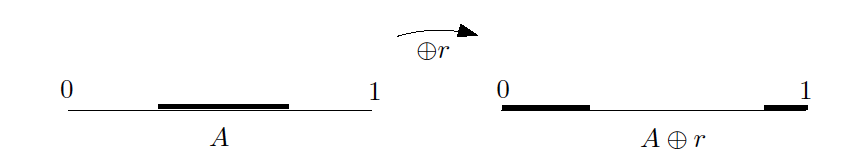
\includegraphics[width=12.06in]{images/basic_shift} 

}

\caption{Shift invariance.}\label{fig:unnamed-chunk-78}
\end{figure}

``wrapping around''를 이용해 \(A\)를 \(r\)만큼 이동해도 길이가 보존되기 때문에, 확률 또한
\[P\{ A \oplus r \}=P\{ A \}, \qquad{\text{for any } 0 < r < 1}\]
이 될 것이라 추론할 수 있다.

이제 모든 \(A \in 2^{[0,1]}\)에 대해 균등확률이 존재하지 않음을 보이기 위해 동치관계(equivalence relation)라는 것에 대해 정의할 것이다. \(x\)와 \(y\) (\(x,y \in [0,1]\))는 \(y-x\in\mathbb{Q}\)를 만족할 경우 동치관계라 정의하고 \(x \sim y\)로 표시한다. 예를 들면
\[\frac{1}{2} \sim \frac{1}{4}, \frac{1}{3} \nsim \frac{1}{\pi}, \frac{1}{\pi}-\frac{1}{4} \sim \frac{1}{\pi}+\frac{1}{2} \]
인 것이다. 이 동치관계는 \([0,1]\)을 다음과 같이 분리(disjoint) 합집합들로 표현할 수 있다. \(\mathbb{Q}_{1}=[0,1]\cap \mathbb{Q}\)라고 하자.우리는 분리 합집합을 다음과 같이 쓸 수 있다.
\[[0,1]=\mathbb{Q}_{1} \cup \{ \bigcup_{x\in [0,1] \backslash \mathbb{Q}_{1}} \{ (\mathbb{Q}+x)\cap [0,1] \} \}=\mathbb{Q}_{1} \cup \{ \bigcup_{x\in [0,1] \backslash \mathbb{Q}_{1}} \{ (\mathbb{Q}+x)\oplus x \} \}.\]

\begin{figure}

{\centering 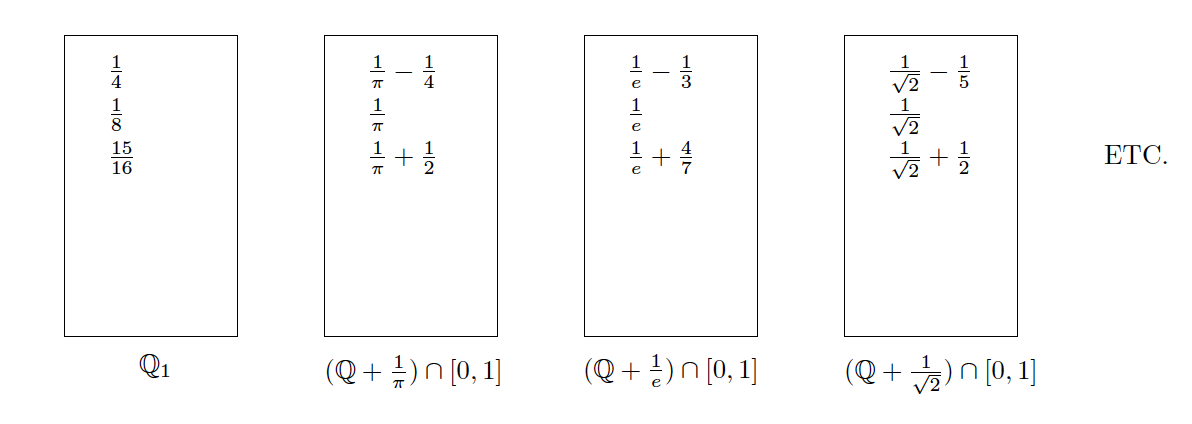
\includegraphics[width=16.56in]{images/basic_disjoint} 

}

\caption{Collection of disjoint unions on [0,1]}\label{fig:unnamed-chunk-79}
\end{figure}

\(H\)를 선택공리(the Axiom of Choice)에 의해 \([0,1]\)의 모든 동치관계에서 원소를 한 개씩 잘 뽑아서 만든 \([0,1]\)의 부분집합이라고 하자. 편의상 \(0\notin H\)라고 하자. 그러면 \((0,1]\)을
\[(0,1]=\bigcup_{r\in\mathbb{Q}_{1}, r\neq 1}\{ H \oplus r\} \qquad{\text{with }\{H\oplus r_{i}\} \cap \{H\oplus r_{j}=\emptyset \text{ for all } i\neq j\} } \]
로 표현할 수 있다. 그러면
\[1=P\{(0,1]\}=P\Big\{ \bigcup_{r\in\mathbb{Q}_{1}, r\neq 1}\{ H \oplus r\} \Big\}=\sum_{r\in \mathbb{Q}_{1},r\neq 1}P\{ H \oplus r\}=\sum_{r\in \mathbb{Q}_{1},r\neq 1}P\{ H\}\]
가 된다. 만약 우리가 \(p=P\{H\}\)로 확률을 부여하고자 한다면

\begin{enumerate}
\def\labelenumi{\arabic{enumi}.}
\item
  \(p=0\)일 때에는 \(1=\sum_{r\in \mathbb{Q}_{1},r\neq 1}P\{ H\}=\sum_{r\in \mathbb{Q}_{1},r\neq 1} p \sum_{r\in \mathbb{Q}_{1},r\neq 1} 0 = 0\) 이므로 모순이다.
\item
  마찬가지로 \(0<p\leq 1\)일 때에는 \(\sum_{r\in \mathbb{Q}_{1},r\neq 1} p =\infty\)이므로 모순이다.
\end{enumerate}

즉 \(H\)는 사건이 아닌 셈이 되고 \(P\{ H \}\)가 존재하지 않는다. 이상의 결과를 다음 정리로 요약해본다.

\BeginKnitrBlock{theorem}[연속 표본공간에서 시그마-체로 멱집합을 쓰지 않는 이유]
\protect\hypertarget{thm:unnamed-chunk-80}{}{\label{thm:unnamed-chunk-80} \iffalse (연속 표본공간에서 시그마-체로 멱집합을 쓰지 않는 이유) \fi{} }셀 수 없는 표본공간 \([0,1]\)에서 시그마-체 \(2^{[0,1]}\)을 고려할 경우 \(P\{[a,b]\}=b-a, \text{ for all } 0\leq a \leq b \leq 1\)과 \(P\{ A \oplus r\}=P\{A\}, \text{ for all } A\subseteq [0,1] \text{ and } 0 < r < 1\)을 동시에 만족하는 \(P: 2^{[0,1]}\rightarrow [0,1]\)은 존재하지 않는다.
\EndKnitrBlock{theorem}

다시말하면, 모든 집합 \(A\subseteq [0,1]\)에 대해 균등확률 \(P\{ A \}\)를 정의할 수 없다는 것이다.

\hypertarget{---borel-sigma-field-on-r}{%
\subsection{실수공간에서 보렐 시그마-체(Borel sigma-field on R)}\label{---borel-sigma-field-on-r}}

따라서, 모든 interval을 포함하는 시그마-체들 중 가장 \textbf{작은} 시그마-체 \(\mathcal{F}\)를 찾는 것이 이상적일 것이다. 즉 우리는 \(\sigma(\text{intervals})\)를 찾고자 하는 것이다.

여기서 잠시 \(\mathbb{R}\)에서의 \textbf{보렐 시그마-체(Borel sigma-algebra)}에 대해 살펴보자. \(\mathbb{R}\)에서의 모든 열린 집합(open set)들의 모임을 \(\mathcal{O}\)라고 하자. 그러면 \(\mathcal{O}\)는 시그마-체가 아니다. (왜냐하면 \(A\in\mathcal{O}\)이면 \(A^{C}\)는 닫힌 집합이고 따라서 \(A^{C}\notin\mathcal{O}\)이다.)

\BeginKnitrBlock{definition}[보렐 시그마-체]
\protect\hypertarget{def:unnamed-chunk-81}{}{\label{def:unnamed-chunk-81} \iffalse (보렐 시그마-체) \fi{} }\(\mathbb{R}\)에서의 \textbf{보렐 시그마-체(Borel sigma-field, Borel sigma-algebra)} \(\mathcal{B}\)는 \(\mathcal{B}=\sigma(\mathcal{O})\)로 정의한다.
\EndKnitrBlock{definition}

결론은 \(\mathbb{R}\)에서의 보렐 시그마-체를 interval을 포함하는 시그마-체로 만들 수 있다는 것이다. 그 전에 증명을 위해 한 가지 정리를 언급하겠다.

\BeginKnitrBlock{theorem}[열린 집합과 열린 구간들]
\protect\hypertarget{thm:unnamed-chunk-82}{}{\label{thm:unnamed-chunk-82} \iffalse (열린 집합과 열린 구간들) \fi{} }\(E \subseteq \mathbb{R}\)이 열린 집합이라고 하자. 그러면 기껏해야 셀 수 있는 정도로만 많은(at most countably many) 열린 구간들(open intervals) \(I_{j}, j=1,2,\ldots,\)가 존재해 다음을 만족한다.
\[E=\bigcup_{j=1}^{\infty}I_{j}.\]
\EndKnitrBlock{theorem}

\BeginKnitrBlock{proof}
\iffalse{} {Proof. } \fi{}이 정리의 증명은 \(E=\bigcup_{j=1}^{\infty}I_{j}\)를 만족하는 \(I_{j}\)들이 있음을 보이고 이것이 (1) at most countably many (2) disjoint (3) open (4) intervals 임을 보이면 된다. 증명 방법은 동치 관계를 이용하는 것이다. \(a, b \in E, (a < b)\)일 때 열린구간 \((a,b)\subseteq E\)이면 \(a \sim b\)로 놓는다. 그러면 \(E\)의 disjoint union of classes는 equivalence relationship partitions \(E\)가 된다. 아직 이것들이 countably many한지 모르므로 이들을 \(I_{j}, j\in J, J \text{ is an arbitrary index set}\)이라고 놓자. 임의의 \(a_{j}<b_{j}\in I_{j}\)에 대해 \(a_{j} \sim b_{j}\)이고 \((a_{j}, b_{j}) \in I_{j}\)이므로 \(I_{j}\)는 interval이다. 또 \(x\in I_{j}\)를 임의로 뽑았을 때 \(x\in E\)이고 \(E\)가 open이므로, \((x-\epsilon, x+\epsilon)\subseteq E\)를 만족하는 \(\epsilon >0\)이 모든 \(x\)에 대해 존재함을 알 수 있고 모든 \(a\in (x-\epsilon, x+\epsilon)\)에 대해 \(a \sim x\)이므로 \(x\)의 \(\epsilon\)-근방은 \(I_{j}\)에 포함됨을 알 수 있어 \(I_{j}\)는 open이다. 마지막으로 모든 \(I_{j}\)는 적어도 하나의 유리수를 포함하고 있어 이를 통해 \(I_{j}\)의 갯수는 countably many임을 알 수 있다.
\EndKnitrBlock{proof}

\BeginKnitrBlock{theorem}[실수 구간에서의 보렐 시그마-체의 생성]
\protect\hypertarget{thm:unnamed-chunk-84}{}{\label{thm:unnamed-chunk-84} \iffalse (실수 구간에서의 보렐 시그마-체의 생성) \fi{} }\(\mathbb{R}\)에서의 보렐 시그마-체(Borel sigma-field, Borel sigma-algebra) \(\mathcal{B}\)는 \((-\infty, a], a\in\mathbb{Q}\)로 생성할 수 있다.
\EndKnitrBlock{theorem}

\BeginKnitrBlock{proof}
\iffalse{} {Proof. } \fi{}\(\mathcal{O}_{0}\)을 \(\mathbb{R}\)에서의 모든 열린 구간(open interval)들의 collection이라고 하자. 앞선 정리에 의해 \(\mathbb{R}\)에서의 모든 열린 집합은 기껏해야 셀 수 있을 정도의 열린 구간의 합집합으로 나타낼 수 있으므로 \(\sigma(\mathcal{O}_{0})=\mathcal{B}\)가 된다. \(\mathcal{D}\)를 \((-\infty, a], a\in \mathbb{Q}\)인 구간들의 collection이라고 하자. 그리고 구간 \((a,b)\)를 \((a,b)\in \mathcal{O}_{0}, a,b \in \mathbb{Q}, a<b\)와 같이 정의하자. 여기서
\[a_{n}=a+\frac{1}{n} \text{ and } b_{n}=b-\frac{1}{n}\]
으로 놓으면
\[(a,b)=\bigcup_{n=1}^{\infty}(a_{n},b_{n}]=\bigcup_{n=1}^{\infty}\{ (-\infty, b_{n}] \cap (-\infty, a_{n}]^{c}\}\]
이다. 이것은 \((a,b)\in \sigma (\mathcal{D})\)임을 의미한다. 즉 \(\mathcal{O}_{0}\subseteq \sigma(\mathcal{D})\)이고 \(\sigma(\mathcal{O}_{0})\subseteq \sigma(\mathcal{D})\)이다. 그러나 \(\mathcal{D}\)의 모든 원소는 닫힌 집합이고 이는 \(\sigma(\mathcal{D})\subseteq \mathcal{B}\)를 의미한다. 따라서
\[\mathcal{B} = \sigma(\mathcal{O}_{0})\subseteq \sigma(\mathcal{D})\subseteq \mathcal{B}\]
이므로 \(\sigma(\mathcal{D})=\mathcal{B}\)이다.
\EndKnitrBlock{proof}

이제 \([0,1]\subset \mathbb{R}\)에서의 보렐 시그마-체 \(\mathcal{B}_{1}\)을 생각해보자. 이는 \(\mathcal{B}\)와 마찬가지로 \([0,1]\)의 열린 부분집합들의 collection으로부터 생성된 시그마-체라고 생각할 수 있다. 한 가지 주의해야 할 점은 \(\mathcal{B}_{1}\)은 \(\mathcal{B}\)의 부분 시그마-체는 아니라는 것이다. 시그마-체에서 포함 관계를 얘기하려면 두 시그마-체의 표본공간이 같아야 한다.

\hypertarget{--construction-of-a-probability-measure-on-r}{%
\subsection{실수공간에서 확률측도의 구성(construction of a probability measure on R)}\label{--construction-of-a-probability-measure-on-r}}

이제 앞서 언급한 보렐 시그마-체 \(\mathcal{B}_{1}\)을 이용해 균등한 확률을 만드는 작업을 진행할 것이다. 전략은 먼저 \textbf{단조족정리(monotone class theorem)}을 증명한 후 그것의 따름정리를 이용해 모든 \(0\leq a \leq b \leq 1\)에서 균등확률 \(P\{[a,b]\}=b-a\)를 정의한 후 이것을 \([0,1]\)의 보렐집합으로 확장하는 것이다.

\(\mathcal{F}_{0}\)를 표본공간 \(\Omega\)에서의 부분집합들의 collection이라고 하자. 그러면 \(\mathcal{F}_{0}\)에서 확률측도 \(P:\mathcal{F}_{0} \rightarrow [0,1]\)을 정의한다. 그리고 \(\mathcal{F}=\sigma(\mathcal{F}_{0})\)의 확률측도 \(Q:\mathcal{F} \rightarrow [0,1]\)가 \(Q\{A\}=P\{A\} \forall A\in \mathcal{F}_{0}\)인 성질을 가진체로 정의된다는 것을 보인다. 마지막으로 이 \(Q\)가 유일함을 보일 것이다.

그 전에 몇 가지 개념들에 대해 정의하겠다.

\BeginKnitrBlock{definition}[유한한 교집합에 대해 닫혀있다]
\protect\hypertarget{def:unnamed-chunk-86}{}{\label{def:unnamed-chunk-86} \iffalse (유한한 교집합에 대해 닫혀있다) \fi{} }표본공간 \(\Omega\)의 부분집합들의 class \(\mathcal{C}\)가
\[\bigcap_{i=1}^{n}A_{i}\in\mathcal{C}\qquad{\text{for every }n\infty \text{ and } A_{1},\ldots ,A_{n}\in\mathcal{C}}\]
를 만족하면 \textbf{유한한 교집합에 대해 닫혀있다(closed under finite intersection)}라고 한다.
\EndKnitrBlock{definition}

\BeginKnitrBlock{definition}[증가하는 극한에 대해 닫혀있다]
\protect\hypertarget{def:unnamed-chunk-87}{}{\label{def:unnamed-chunk-87} \iffalse (증가하는 극한에 대해 닫혀있다) \fi{} }표본공간 \(\Omega\)의 부분집합들의 class \(\mathcal{C}\)가
\[\bigcup_{i=1}^{\infty}A_{i}\in\mathcal{C}\qquad{\text{for every collection } A_{1}, A_{2},\ldots \in \mathcal{C} \text{ with } A_{1}\subseteq A_{2}\subseteq \ldots}\]
를 만족하면 \textbf{증가하는 극한에 대해 닫혀있다(closed under increasing limits)}라고 한다.
\EndKnitrBlock{definition}

\begin{figure}

{\centering 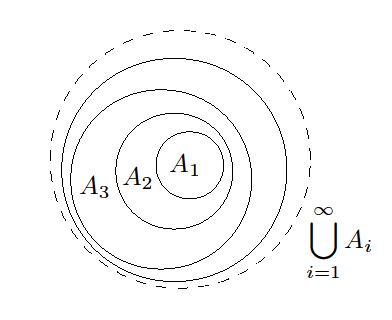
\includegraphics[width=5.44in]{images/basic_cuil} 

}

\caption{Closed under increasing limits.}\label{fig:unnamed-chunk-88}
\end{figure}

\BeginKnitrBlock{definition}[유한한 차에 대해 닫혀있다]
\protect\hypertarget{def:unnamed-chunk-89}{}{\label{def:unnamed-chunk-89} \iffalse (유한한 차에 대해 닫혀있다) \fi{} }표본공간 \(\Omega\)의 부분집합들의 class \(\mathcal{C}\)가 모든 \(A,B\in\mathcal{C}, A\subseteq B\)에 대해 \(B\backslash A \in \mathcal{C}\)를 만족하면 \textbf{유한한 차에 대해 닫혀있다(closed under finite differences)}라고 한다.
\EndKnitrBlock{definition}

\begin{figure}

{\centering 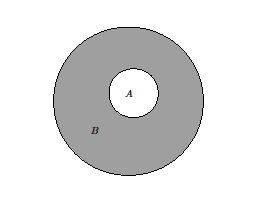
\includegraphics[width=3.67in]{images/basic_cufd} 

}

\caption{Closed under finite differences.}\label{fig:unnamed-chunk-90}
\end{figure}

다음은 단조족에 대한 정의다.

\BeginKnitrBlock{definition}[단조족]
\protect\hypertarget{def:unnamed-chunk-91}{}{\label{def:unnamed-chunk-91} \iffalse (단조족) \fi{} }표본공간 \(\Omega\)의 부분집합들의 class \(\mathcal{C}\)가 closed under countable increasing set이거나 closed under countable decreasing set이면, 즉 \(E_{1},E_{2},\ldots \in \mathcal{C}\)일 때
\[E_{i}\uparrow E \text{ or } E_{i}\downarrow E \Longrightarrow E \in \mathcal{C}\]
이면 \(\mathcal{C}\)를 \textbf{단조족(monotone class)}이라고 한다.
\EndKnitrBlock{definition}

이에 대한 증명은 \citep{Durrett2010}의 Appendix 부분을 참고하자.

\hypertarget{rv}{%
\chapter{확률변수}\label{rv}}

\textbf{확률변수(random variable)}의 예로는 카드를 생각해 볼 수 있다. 확률변수 \(X=X(\omega)\)는 실변수 함수로 정의역은 \(\Omega\)이다. 각각의 \(\omega\)가 특정한 5장의 카드 집합을 나타낸다고 할 때 \(X(\omega)=I\{\omega\)가 네 개의 에이스를 가지고 있음\(\}\)이라고 정의한다면 \(X(\omega)\)는 random variable이다.

\BeginKnitrBlock{definition}[가측]
\protect\hypertarget{def:unnamed-chunk-92}{}{\label{def:unnamed-chunk-92} \iffalse (가측) \fi{} }\((\Omega_{1}, \mathcal{F}_{1})\), \((\Omega_{2}, \mathcal{F}_{2})\)가 두 가측공간(measurable)이라고 할 때, 함수 \(X:\Omega_{1} \rightarrow \Omega_{2}\)가 임의의 집합 \(E\in \mathcal{F}_{2}\)에 대해 집합 \(X^{-1}(E)\)이
\[X^{-1}(E)=\{ \omega \in \Omega_{1}: X(\omega) \in E\} \mathcal{F}_{1}\]
(또는 위 조건을 \(X^{-1}(\mathcal{F}_{2})\in \mathcal{F}_{1})\))
일 때 \(X\)가 \textbf{가측(measurable)}이라고 한다. (또는 \(\mathcal{F}_{1}\)-가측 이라고도 부른다.)
\EndKnitrBlock{definition}

\BeginKnitrBlock{definition}[확률변수]
\protect\hypertarget{def:unnamed-chunk-93}{}{\label{def:unnamed-chunk-93} \iffalse (확률변수) \fi{} }\((\Omega, \mathcal{F}, P)\)가 확률공간(probability space)이라고 하자. 그러면 어떤 실변수 함수
\[X:\Omega \rightarrow \mathbb{R}\]
가 \((\Omega, \mathcal{F})\)에서 \((\mathbb{R}, \mathcal{B})\)로 가는 가측함수(measurable function)일 때(여기서 \(\mathcal{B}\)는 \(\mathbb{R}\)에서의 보렐 시그마-체) 이 \(X\)를 \textbf{확률변수(random variable)}라고 부른다.
\EndKnitrBlock{definition}

다음 그림은 \((\Omega, \mathcal{F}, P)= ((0,1), \mathcal{B}_{(0,1)}, \mu_{L})\)에서의 확률변수 \(X(\omega) = \frac{1}{\omega(1-\omega)}\)의 \textbf{역상(inverse image)} 개념을 묘사한 것이다. 이 때 보렐 집합 \(B=\{ (6.25, \infty)\cup \{4\} \}\)이며, \(X^{-1}(B)=\{ (0,0.2)\cup (0.8,1)\cup \{0.5\} \}\)이며 이는 \(\mathcal{B}_{(0,1)}\)안에 있다.

\begin{figure}

{\centering 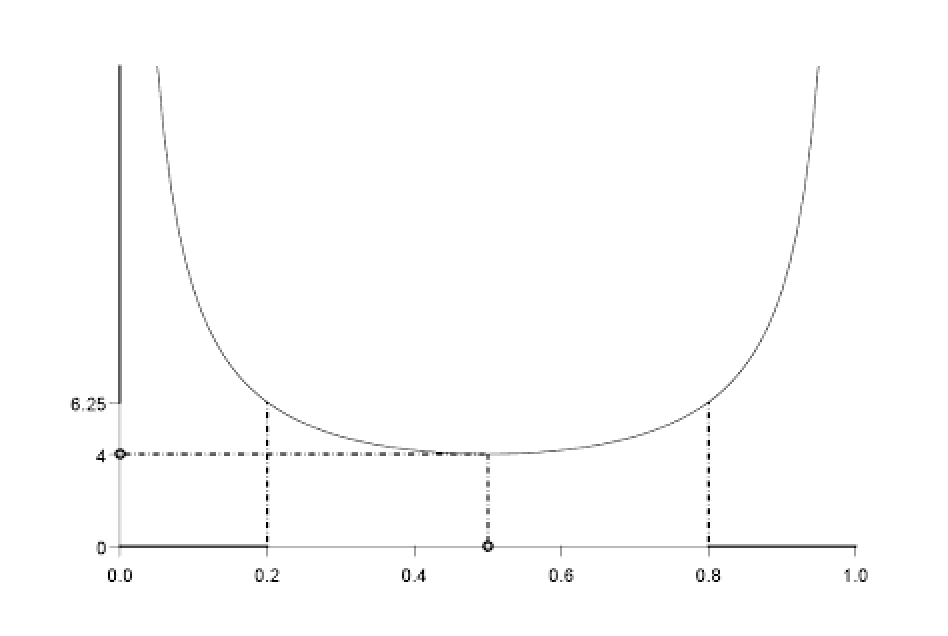
\includegraphics[width=13.17in]{images/basic_invimage} 

}

\caption{역상의 예.}\label{fig:unnamed-chunk-94}
\end{figure}

\BeginKnitrBlock{example}[확률변수의 예]
\protect\hypertarget{exm:unnamed-chunk-95}{}{\label{exm:unnamed-chunk-95} \iffalse (확률변수의 예) \fi{} }\(\Omega=[0,1]\), \(\mathcal{F}=\mathcal{B}_{[0,1]}\)이며 \(\Omega\)의 부분집합이라고 하자. 그러면

\begin{enumerate}
\def\labelenumi{\arabic{enumi}.}
\item
  \(X_{1}(\omega)\equiv=c\).
\item
  \(X_{2}(\omega)=I(\omega \leq 1/2)\).
\item
  \(X_{3}(\omega) = \omega\).
\end{enumerate}

위 \(X_{1}\), \(X_{2}\), \(X_{3}\)은 모두 확률변수이다. \(B\in\mathcal{B}\)이면 \(B\)가 \(c\)를 포함할 경우 \(X_{1}^{-1}(B)=\Omega\in\mathcal{F}\), 그렇지 않을 경우 \(X_{1}^{-1}(B)=\emptyset\in\mathcal{F}\)이므로 \(X_{1}\)는 \(\mathcal{F}\)-가측이다. 또한
\[
X_{2}^{-1}(B) := 
\begin{cases}
\emptyset\in\mathcal{F} & \text{if $B$ contains neither 0 nor 1} \\
\Omega\in\mathcal{F} & \text{if $B$ contains both 0 and 1} \\
[1/2,1]\in\mathcal{F} & \text{if $B$ contains 1, but not 0} \\
[0,1/2]\in\mathcal{F} & \text{if $B$ contains 0, but not 1} \\
\end{cases}
\]
이며 따라서 \(X_{2}\)는 \(\mathcal{F}\)-가측이다. \(B\in\mathcal{B}\)일 떄 \(X_{3}^{-1}(B)=B\cap [0,1] \in \mathcal{B}_{[0,1]}\in\mathcal{F}\)이므로 \(X_{3}(\omega)\)또한 확률변수다.
\EndKnitrBlock{example}

앞선 예제에서 \(X\)가 확류변수임을 보이기 위해 \(X^{-1}(\mathcal{B})=\{ X^{-1}(B), B\in\mathcal{B}\}\)를 계산하였다. 이 때 \(\mathcal{F}\)의 부분집합인 \(X^{-1}(\mathcal{B})\)는 \(X\)를 가측으로 만드는 관점에서 가장 작은 시그마-장이된다.

\BeginKnitrBlock{definition}[확률변수로부터 생성되는 시그마-장]
\protect\hypertarget{def:unnamed-chunk-96}{}{\label{def:unnamed-chunk-96} \iffalse (확률변수로부터 생성되는 시그마-장) \fi{} }만약 \(X\)가 확률변수라면, \(X\)를 가측으로 만드는 가장 작은 시그마-장, 즉 \(X^{-1}(\mathcal{B})=\{ X^{-1}(B), B\in\mathcal{B}\}\)를 \(X\)로부터 생성되는 시그마-장이라 하고 \(\sigma(X)\)라 표기한다.
\EndKnitrBlock{definition}

앞선 예제에서 확률변수 \(X\)에 대해 사건 \(F\in \sigma(X)\)을 결정할 수 있다. 예를 들면, \(\sigma(X_{1})=\{ \emptyset, [0,1] \}\subset \{ \emptyset, [0,1], [0,1/2), [1/2,1] \}=\sigma(X_{2})\)이다. 이 말은 \(X_{2}\)가 \(X_{1}\)보다 \(\omega\)에 대해 더 많은 정보를 준다는 것을 말해준다. \(X_{1}\)은 어떤 사건이 일어났는지 안일어났는지만 얘기해주지만, \(X_{2}\)는 \(\omega\)가 1/2보다 큰지 작은지도 알려주는 것이다. 또한 \(\sigma(X_{2})\subset\sigma(X_{3})\)이므로 \(X_{3}\)은 \(X_{2}\)보다 많은 정보를 주는 것이다. 실제로 \(X_{3}\)은 실험에서 나온 \(\omega\)의 정확한 값을 알려준다.

\BeginKnitrBlock{definition}[보렐 측도가능과 르베그 측도가능 함수]
\protect\hypertarget{def:unnamed-chunk-97}{}{\label{def:unnamed-chunk-97} \iffalse (보렐 측도가능과 르베그 측도가능 함수) \fi{} }어떤 함수 \(f:\mathbb{R}^{k}\rightarrow \mathbb{R}\)을

\begin{enumerate}
\def\labelenumi{\arabic{enumi}.}
\item
  1차원 보렐 집합 \(B\in\mathcal{B}\)에 대해 \(f^{-1}*B\) 가 \(k\)차원 보렐 집할이 될 경우 \textbf{보렐 측도가능(Borel measurable)} 또는 \textbf{보렐 함수(Borel function)}이라고 부른다.
\item
  1차원 르베그 집합 \(B\in\mathcal{B}\)에 대해 \(f^{-1}*B\) 가 \(k\)차원 르베그 집할이 될 경우 \textbf{르베그 측도가능(Lebesgue measurable)} 또는 \textbf{르베그 함수(Lebesguel function)}이라고 부른다.
\end{enumerate}
\EndKnitrBlock{definition}

\hypertarget{---borel-cantelli-lemma}{%
\section{보렐-칸텔리 따름정리 (Borel-Cantelli lemma)}\label{---borel-cantelli-lemma}}

\BeginKnitrBlock{lemma}[보렐-칸텔리 따름정리]
\protect\hypertarget{lem:unnamed-chunk-98}{}{\label{lem:unnamed-chunk-98} \iffalse (보렐-칸텔리 따름정리) \fi{} }\textbf{(Borel-Cantelli lemma)} 만약 \(\sum_{n=1}^{\infty}P(A_{n}) < \infty\)라면
\[P(A_{n} i.o.)=0\]
이다.
\EndKnitrBlock{lemma}

\BeginKnitrBlock{lemma}[제 2 보렐-칸텔리 따름정리]
\protect\hypertarget{lem:unnamed-chunk-99}{}{\label{lem:unnamed-chunk-99} \iffalse (제 2 보렐-칸텔리 따름정리) \fi{} }\textbf{(Second Borel-Cantelli lemma)} 만약 사건 \(A_{n}\)들이 독립이라면 \(\sum P(A_{n})=\infty\)는 \(P(A_{n} i.o.)=1\)임을 내포한다.
\EndKnitrBlock{lemma}

\hypertarget{expectation}{%
\chapter{적분과 기댓값}\label{expectation}}

\hypertarget{riemann-integral}{%
\section{리만적분(Riemann integral)}\label{riemann-integral}}

구간 \([a,b]\)에서 함수 \(f(x)\)의 \textbf{리만적분(Riemann integral)}은 부분합의 극한으로 정의된다. 우리는 구간 \([a,b]\)를 \(a=x_{0}<x_{1}<\ldots <x_{n} =b\)로 나무어 다음과 같은 합을 만들 수 있다.

\begin{equation}
\sum_{i=1}^{n}f(\xi_{i})\Delta x_{i}.
 \label{eq:Riemannintegral}
\end{equation}

이 때 \(\xi_{i}\)는 \(i\)번째 구간 \([x_{i-1},x_{i})\)에 있는 점이며 \(\Delta x_{i}=x_{i}-x_{i-1}\)이다. \(\xi_{i}\)와 \(\Delta x_{i}\)는 \(n\)과도 관련이 있음을 알아두자. 그러나 표기의 간편성을 위해 생략하기로 한다. 그러면 \(\xi_{i}\)를 어떻게 선택하는지와 상관없이 \(n\rightarrow\infty\)이고 \(\max_{1\leq i \leq n}\Delta x_{i} \rightarrow 0\)일 때 \(f\)를 \textbf{리만적분 가능(Riemann integrable)}하다고 말한다.

리만적분성은 \(f\)가 꽤 regular함을 요구한다. \(x\)가 유리수일 때 0, 아닐때 1을 갖는 함수 \(f(x)\)가 있다고 하자. 그러면 식 \eqref{eq:Riemannintegral}의 극한 \(\int_{0}^{1}f(x)dx\)는 중간값을 어떻게 고르냐에 따라 값이 달라지므로 리만적분 가능하지 않다. 모든 \(i\)에 대해 \(\xi_{i}\)를 유리수로 고르면 극한의 0이되나, 반대로 모든 \(i\)에 대해 무리수로 \(\xi_{i}\)를 잡을 경우 극한은 1이 된다. 그리고 \(xi_{i}\)를 유리수와 무리수를 섞어 잡을 경우 극한은 존재하지 않게 된다.

\hypertarget{-lebesgue-integral}{%
\section{르베그 적분(Lebesgue integral)}\label{-lebesgue-integral}}

적분을 정의하는 또 다른 방법으로 \(x\)축대신 \(y\)축을 등간격으로 잘라 부분학의 극한을 구하는 방법이 있다.

\begin{equation}
\sum_{i=1}^{\infty}y_{i}\mu\{ f^{-1}(A_{i}) \}.
 \label{eq:Lebesgueintegral}
\end{equation}

이 때 \(y_{i}\)는 \(i\)번째 \(y\)구간에서의 점을 나타내며 \(\mu\)는 \textbf{르베그 측도(Lebesgue measure)}가 된다. 즉, 각각의 \(y\) 구간에 대해 우리는 중간값 \(y_{i}\)를 취하며 \(A_{i}\)에 대한 \(f\)의 역상 \(f^{-1}(A_{i})\)의 르베그 측도로 곱한다. 아래 그림에서는 \(f^{-1}(A_{i}) = [a,b]\cup [c,d]\)이다. 그리고 이에 대응되는 르베그 측도는 \(\mu\{f^{-1}(A_{i}) \}= (d-c) + (b-a)\)이다. 결국 해당 부분의 부분합은 \(y_{i} \times \{ (d-c) + (b-a)\}\)인 것이다. 이런 방식의 적분을 \textbf{르베그 적분(Lebesgue integral)}이라고 부른다.

\begin{figure}

{\centering 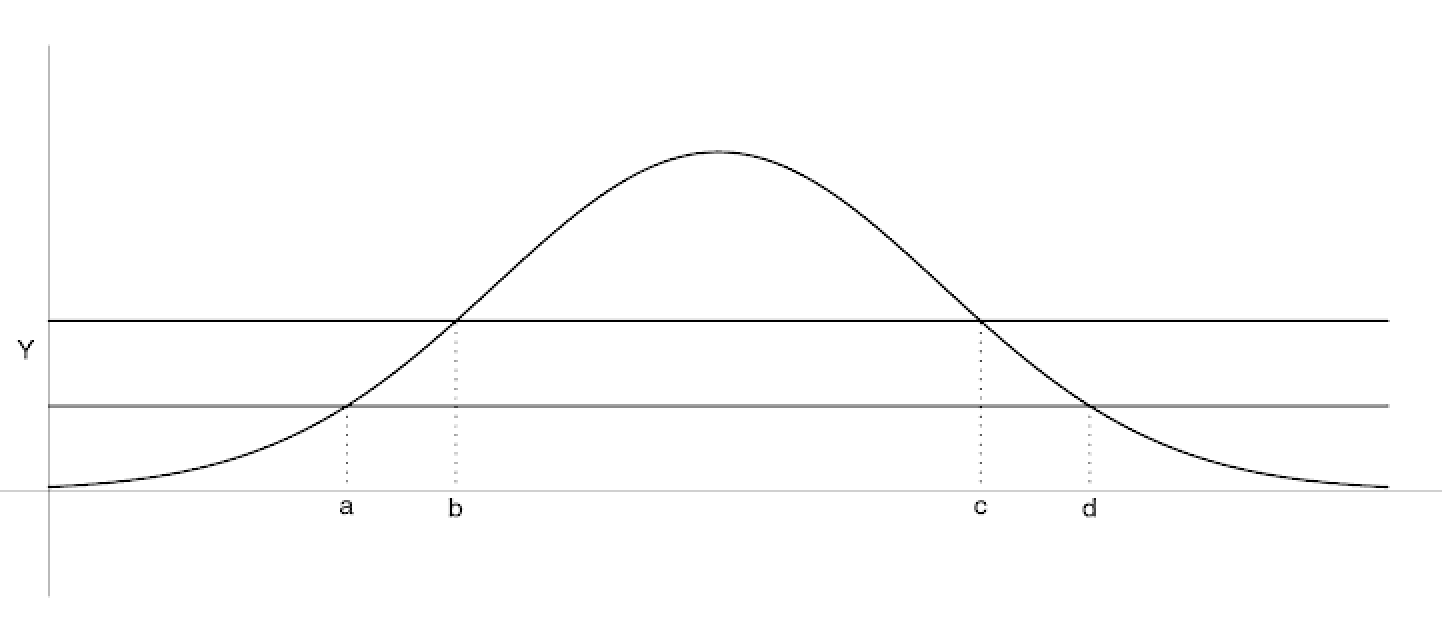
\includegraphics[width=20.03in]{images/math_Lebesgue} 

}

\caption{가로선은 y를 등간격으로 잘라낸 구간 A를 의미한다. 그러면 A의 inverse image of f는 [a,b]와 [c,d]의 합집합에 대응된다.}\label{fig:unnamed-chunk-100}
\end{figure}

\(x\)축 대신 \(y\)축을 분할하는 것의 장점은 \(f\)가 \(x\)에 대해 더이상 잘 행동하는 함수일 필요가 없다는 것이다. 다시 앞서 리만 적분에서 등장한 적분 문제를 생각해보자. \(A_{i}\)와 \(A_{j}\)를 각각 \(y=0\), \(y=1\)에 대응되는 구간이라고 한다면 앞서 적분 식 \eqref{eq:Lebesgueintegral}은 \(y_{i}\mu\{ f^{-1}(A_{i}) \} + y_{j}\mu\{ f^{-1}(A_{j}) \}\)가 된다. 이 때 \(y_{i}\), \(y_{j}\)는 \(A_{i}\), \(A_{j}\)의 중간값에 해당된다. \(f^{-1}(A_{i})\)과 \(f^{-1}(A_{j})\)는 각각 \([0,1]\)에서 유리수와 무리수의 집합에 대응되며 그들의 르베그 적분은 각각 0과 1이다. 따라서 최종 르베그 적분값 \(\int_{0}^{1}f(x)dx\)는 존재하며 1이다.

\begin{figure}

{\centering 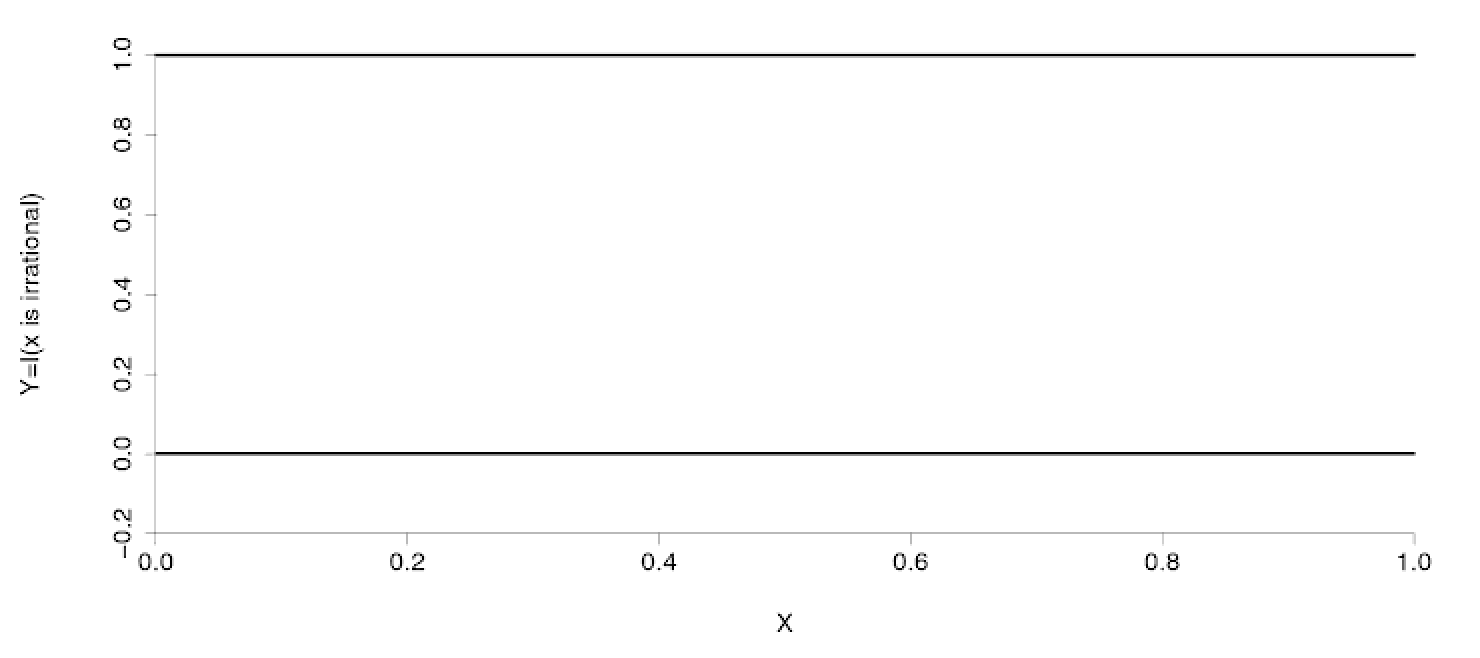
\includegraphics[width=20.56in]{images/math_irrationalintegral} 

}

\caption{x가 무리수와 유리수일 때 1, 0을 주는 함수의 적분을 생각해보자. 르베그 적분의 방법으로 y축을 분할하면 충분히 작은 구간에서 함수값이 0인 경우와 1인 경우를 분리시킬 수 있다. 그 다음에는 구간 [0,1] 사이에서의 무리수들의 집합의 르베그 측도(1)와 유리수들의 집합의 르베그 측도(0)을 재면 된다.}\label{fig:unnamed-chunk-101}
\end{figure}

이것을 더 확장하여 선으로 정의된 공간이 아닌 임의의 공간 \(\Omega\)에서 정의된 르베그 측도뿐 아니라 임의의 측도 \(\mu\)에 대해서 \(f\)의 적분 또한 정의할 수 있다. 만약 \(\mu\)가 확률공간 \(\Omega\)에서 정의된 측도라고 한다면, 우리는 적분을 다음과 같이 정의할 수 있다.
\[\int f(\omega)d\mu (\omega).\]
이것은 \(y\)축을 등간격으로 분할하고 \eqref{eq:Lebesgueintegral}처럼 합을 취한 후 \(y\)축의 분할 넓이가 0이 되도록 극한을 취함으로써 얻을 수 있다. 그런데 이 적분에는 두 가지 문제가 있다.

\begin{enumerate}
\def\labelenumi{\arabic{enumi}.}
\item
  극한이 존재하지 않을 수도 있고
\item
  극한이 중간값 \(y_{i}\)를 어떻게 고르는지에 따라 바뀔 수도 있다.
\end{enumerate}

이러한 문제점은

\begin{enumerate}
\def\labelenumi{\arabic{enumi}.}
\item
  \(f\)를 음이 아닌 함수로 정의하고
\item
  \(y\)를 분할하는 구간을 현명하게 자름으로써 피할 수 있다.
\end{enumerate}

\hypertarget{--lebegue-stieltjes-integration}{%
\section{르베그-스틸체스 적분(Lebegue-Stieltjes Integration)}\label{--lebegue-stieltjes-integration}}

\((\Omega, \mathcal{F}, \mu)\)를 측도 공간(measure space)라고 하고 \(f(\omega): \Omega \rightarrow \mathbb{R}\)을 음이 아니고 유한한 값을 갖는 \(\mathcal{F}\)-가측 함수라고 하자. 여기서 \(\mathcal{F}\)-가측이라는 것은 직선위에서의 모든 보렐 구간 \(B\)에 대해 \(f^{-1}(B)\in\mathcal{F}\)인 것을 의미한다. 이 절에서는 \(f\)의 \textbf{르베그-스틸체스 적분(Lebegue-Stieltjes Integration)}을 단계별로 정의한다.

\begin{enumerate}
\def\labelenumi{\arabic{enumi}.}
\item
  \(y\)축을 길이가 1인 구간들로 나눈다. 즉 \(A_{0i}=[i-1,i),i=1,2,\ldots\)로 나누는 것이다. 그리고 \eqref{eq:Lebesgueintegral}을 참고하여 부분합을 만든다. 이 때 \(y_{i}\)는 \(A_{0i}\)에서 가장 작은 값인 \(i-1\)로 둔다.
  \[S_{0} = \sum_{i=1}^{\infty}(i-1)\mu_{0i}.\]
  이 때 \(\mu_{0i}=\mu\{\omega: f(\omega) \in A_{0i} \}\)이다.
\item
  각각의 \(A_{0i}\)를 반으로 나눈다. 즉 \$A\_\{1i\}={[}\frac{i-1}{2}, \frac{i}{2}), i=1,2,\ldots \$를 만드는 것이다. 다시 한 번 \eqref{eq:Lebesgueintegral}을 참고하여 부분합을 만든다. 이 때 \(y_{i}\)는 \(A_{1i}\)에서 가장 작은 값으로 정의한다. 그러면 다음이 생성된다.
  \[S_{1} =\sum_{i=1}^{\infty}\{\frac{i-1}{2}\}\mu_{1i}.\]
  이 때 \(\mu_{1i}=\mu\{\omega: f(\omega)\in A_{1i}\}\)이며 \(S_{0}\leq S_{1}\)이다.
\item
  구간을 반으로 나누고 \eqref{eq:Lebesgueintegral}을 참고하여 부분합을 만드는 과정을 계속 반복한다. \(m\)번째 단계에서 우리는 \(A_{mi}=[\frac{i-1}{2^{m}},\frac{i}{2^{m}})\)으로 놓고
  \[S_{m} =\sum_{i=1}^{\infty}\{\frac{i-1}{2^{m}}\}\mu_{mi}\]
  로 둔다. 이 떄 \(\mu_{mi}=\mu\{\omega: f(\omega)\in A_{mi}\}\)이며 또한 \$S\_\{0\}\leq S\_\{1\}\leq \ldots S\_\{m\} \leq \$가 된다.
\end{enumerate}

\hypertarget{-properties-of-integration}{%
\section{적분의 성질(properties of integration)}\label{-properties-of-integration}}

어떤 상황에서 적분과 극한의 순서를 바꿀 수 있을까?

\BeginKnitrBlock{theorem}[단조수렴정리(MCT)]
\protect\hypertarget{thm:unnamed-chunk-102}{}{\label{thm:unnamed-chunk-102} \iffalse (단조수렴정리(MCT)) \fi{} }
1. null set \(N\) \((\mu(N)=0)\) 바깥의 \(\omega\)에 대해 \(f_{n}(omega)\geq 0,\forall n\)이고 \(f_{n}(\omega)\uparrow f(\omega)\)라고 하자. 그러면 \(\int f_{n}(\omega)d(\omega)\uparrow \int f(\omega)d\mu(\omega)\)이다.

\begin{enumerate}
\def\labelenumi{\arabic{enumi}.}
\setcounter{enumi}{1}
\tightlist
\item
  확률변수 버전으로는, 만약 모든 \(n\)에 대해 \(P\{\omega: X_{n}(\omega)\geq 0 \forall n \text{ and } X_{n}(\omega)\uparrow X(\omega)\}=1\)이라고 하자. 그러면 \(E(X_{n})\uparrow E(X)\)이다.
\end{enumerate}
\EndKnitrBlock{theorem}

\BeginKnitrBlock{theorem}[지배수렴정리(DCT)]
\protect\hypertarget{thm:unnamed-chunk-103}{}{\label{thm:unnamed-chunk-103} \iffalse (지배수렴정리(DCT)) \fi{} }
1. null set \(N\) \((\mu(N)=0)\) 바깥의 \(\omega\)에 대해 \(f_{n}(omega) \rightarrow f(\omega)\)이고 \(|f_{n}(\omega) | \leq g(\omega)\), \(\int g(\omega)d\mu(\omega) < \infty\)일 때 \(\int f_{n}(\omega)d\mu(\omega) \rightarrow \int f(\omega)d\mu(\omega)\)이다.

\begin{enumerate}
\def\labelenumi{\arabic{enumi}.}
\setcounter{enumi}{1}
\tightlist
\item
  확률변수 버전으로는, 만약 모든 \(n\)에 대해 \(P\{\omega: X_{n}(\omega)\rightarrow X(\omega) \text{ and } |X_{n}(\omega)|\leq Y(\omega) \forall n\}=1\)이고 \(E(Y)<\infty\)라고 하자. 그러면 \(E(X_{n})\rightarrow E(X)\)이다.
\end{enumerate}
\EndKnitrBlock{theorem}

지배수렴정리의 따름정리로 유계수렴정리(bounded convergence theorem, BCT)가 있다.

\BeginKnitrBlock{theorem}[유계수렴정리(BCT)]
\protect\hypertarget{thm:unnamed-chunk-104}{}{\label{thm:unnamed-chunk-104} \iffalse (유계수렴정리(BCT)) \fi{} }\(X_{n}\)이 확률변수이고 \(P\{X_{n}(\omega)\rightarrow X(\omega)\}=1\)이며 각 \(n\)에 대해 \(P\{|X_{n}|\leq c\}=1\) 일 때 (\(c\)는 상수), \(E(X_{n})\rightarrow E(X)\)이다.
\EndKnitrBlock{theorem}

\BeginKnitrBlock{remark}
\iffalse{} {Remark. } \fi{}MCT와 DCT는 모든 적분에 대해 적용할 수 있음을 알아내는 것이 중요하다. 합들(sums)은 counting measure에 대한 적분들이므로 이것들에 대해서도 적용할 수 있다.
\EndKnitrBlock{remark}

\hypertarget{inequalities}{%
\section{부등식들(inequalities)}\label{inequalities}}

확률론에서 부등식들은 중요한 역할을 하는데, 대부분의 일들은 다른 것들로부터 특정한 확률로 추정하는 문제들을 다루고 있기 때문이다.

\BeginKnitrBlock{lemma}[모멘트로부터 꼬리확률을 추정]
\protect\hypertarget{lem:unnamed-chunk-106}{}{\label{lem:unnamed-chunk-106} \iffalse (모멘트로부터 꼬리확률을 추정) \fi{} }\(g\)가 음이 아니고, 감소하지 않는 함수이며 \(E\{g(X)\}<\infty\)라고 하자. \(x>0\)일 때
\[P(|X|>x)\leq \frac{E\{g(|X|)\}}{g(x)}\]
이다.
\EndKnitrBlock{lemma}

\BeginKnitrBlock{proof}
\iffalse{} {Proof. } \fi{}\begin{eqnarray}
E\{g(|X|)\} &=& E\{g(|X|)\}I\{|X|>x\}\\
&=& g(x)EI\{|X|>x\}\\
&=& g(x)P(|X|>x).
\end{eqnarray}
\EndKnitrBlock{proof}

\(g\)를 특수하게 설정할 경우 다음 정리를 얻는다.

\BeginKnitrBlock{theorem}[마르코프 부등식]
\protect\hypertarget{thm:unnamed-chunk-108}{}{\label{thm:unnamed-chunk-108} \iffalse (마르코프 부등식) \fi{} }어떤 \(r>0\)에 대해 \(E|X|^{r}<\infty\)라고 하자. 만약 \(x>0\)이면 다음 부등식이 성립한다.
\[P(|X|>x)\leq \frac{E|X|^{r}}{x^{r}}.\]
\EndKnitrBlock{theorem}

\BeginKnitrBlock{corollary}[체비셰프 부등식]
\protect\hypertarget{cor:unnamed-chunk-109}{}{\label{cor:unnamed-chunk-109} \iffalse (체비셰프 부등식) \fi{} }만약 \(X\)가 평균 \(\mu\), 분산 \(\sigma^{2}\)을 갖는 확률변수라면 \(c>0\)에 대해 \(P(|X-\mu|\geq c) \leq \sigma^{2}/c^{2}\)이다.
\EndKnitrBlock{corollary}

\BeginKnitrBlock{theorem}[젠슨 부등식]
\protect\hypertarget{thm:unnamed-chunk-110}{}{\label{thm:unnamed-chunk-110} \iffalse (젠슨 부등식) \fi{} }\(f(x)\)가 convex 함수이고 \(X\)는 유한한 평균 \(\mu\)를 갖는 확률변수라고 하자. 만약 \(E(|f(X)|)<\infty\)이면, \(E\{f(X)\}\geq f\{E(X) \}\)이다.
\EndKnitrBlock{theorem}

\BeginKnitrBlock{corollary}[젠슨 부등식의 따름정리]
\protect\hypertarget{cor:unnamed-chunk-111}{}{\label{cor:unnamed-chunk-111} \iffalse (젠슨 부등식의 따름정리) \fi{} }만약 \(X\)가 어떤 확률변수이고 \(p\geq 1\)이면 \(E(|X|)\leq \{ E(|X|^{p}) \}^{1/p}\)이다.
\EndKnitrBlock{corollary}

\hypertarget{convergencerv}{%
\chapter{확률변수의 수렴}\label{convergencerv}}

\citep{Proschan2016}의 내용을 따라간다. 통계적 추론에서 가장 중요한 부분 중 하나는 추정량 \(\hat{\theta}_{n}\)에서 \(n\rightarrow\infty\)일 때 어떤 일이 일어나는지 살펴보는 것이다. 많은 다른 질문들을 생각해 볼 수 있다. 첫째로, \(\hat{\theta}_{n}\)이 \(n\rightarrow\infty\)일 때 진짜 모수 \(\theta\)에 ``가까이'' 가는가에 대해 생각해 볼 수 있다. 이 ``가까이'' 라는 개념을 세 가지 정도로 정의할 수 있다.

\begin{enumerate}
\def\labelenumi{\arabic{enumi}.}
\item
  \(\theta_{n}\)이 \(\theta\)에 확률 1로 수렴한다.
\item
  어떤 주어진 \(\epsilon >0\)에 대해 \(\hat{\theta}_{n}\) 이 \(\theta\)와 \(\epsilon\) 거리 이내에 위치할 확률이 1이다.
\item
  기댓값 \(|\hat{\theta}_{n}-\theta|^{p}\)가 0으로 수렴한다.
\end{enumerate}

이것들을 차례로 \textbf{거의 확실한 수렴(Almost sure convergence)}, \textbf{확률수렴(Convergence in probability)} 그리고 \textbf{Lp 수렴(Convergence in Lp)}이라고 부른다.

\hypertarget{--almost-sure-convergence}{%
\section{거의 확실한 수렴(Almost sure convergence)}\label{--almost-sure-convergence}}

\(X_{1}, X_{2},\ldots\)가 확률공간 \((\Omega, \mathcal{F}, P)\)에서의 확률변수의 수열이라고 하자. 고정된 \(\omega\)에 대해 \(X_{n}(\omega)=x_{n}, n=1,2,\ldots\)은 숫자의 수열이라고 하자. 각 \(\omega\)에 대해 \(X_{n}(\omega)\)가 수렴할 수 있지만 극한 \(X(\omega)\)는 \(\omega\)에 따라 다를 수 있다. 예를 들면, \((\Omega, \mathcal{F}, P)=([0,1],\mathcal{B}_{[0,1]},\mu_{L})\) 이고

\begin{equation}
X_{n}(\omega)=\omega^{n}
\label{eq:almostsureex01}
\end{equation}

이다. 그러면 \(n\rightarrow \infty\)일 때 \(X_{n}(\omega) \rightarrow I(\omega=1)\)이다. 그런데 어떤 \(\omega\)에 대해서는 \(X_{n}(\omega)\)는 극한이 없거나 무한대의 극한을 갖을 수 있다. 예를 들면 앞선 식 \eqref{eq:almostsureex01}을 다음과 같이 바꾸는 것이다.

\begin{equation}
X_{n}(\omega)=(-\omega)^{n}
\label{eq:almostsureex02}
\end{equation}

그러면 \(\omega < 1\)일 때 \(n\rightarrow 0\)이나 \(\omega=1\)일 때는 극한이 존재하지 않는다.

식 \eqref{eq:almostsureex01}과 \eqref{eq:almostsureex02}에서의 행동이 다르다고 하더라도 \(\{\omega=1\}\)이 확률 0을 갖는다면 다른 행동을 무시할 수 있을 것이다. 이것을 확장시키면 확률 0인 집합들을 무시하는 것으로 이해할 수 있고, \textbf{거의 확실한 수렴(Almost sure convergence)}의 정의를 이끈다.

\BeginKnitrBlock{definition}[거의 확실한 수렴]
\protect\hypertarget{def:unnamed-chunk-112}{}{\label{def:unnamed-chunk-112} \iffalse (거의 확실한 수렴) \fi{} }
1. 확률변수들 \(X_{1}(\omega), X_{2}(\omega), \ldots\)가 \(X(\omega)\)로 거의 확실한 수렴을 한다는 것은, 확률이 0인 집합을 제외한 나머지 부분에서 고정된 \(\omega\)에 대해 숫자들의 수열 \(X_{n}(\omega)\)가 \(n\rightarrow\infty\)함에 따라 \(X(\omega)\)로 수렴하는 것을 의미한다. 특별히 이것을 \(X_{n}\rightarrow X a.s.\) 또는 \(X_{n}\stackrel{a.s.}{\rightarrow}X\)라고 쓴다.

\begin{enumerate}
\def\labelenumi{\arabic{enumi}.}
\setcounter{enumi}{1}
\tightlist
\item
  임의의 측도 공간 \((\Omega, \mathcal{F}, \mu)\)위의 함수들 \(f_{1}(\omega), f_{2}(\omega),\ldots\)의 수열이 \(f(\omega)\)로 거의 확실한 수렴을 한다(converges almost everywhere)는 것은 \(\mu\)-측도가 0인 집합 밖에 있는 모든 \(\omega\)에 대해 실수 수열 \(f_{n}(\omega)\)가 \(f(\omega)\)로 수렴함을 의미한다.
\end{enumerate}
\EndKnitrBlock{definition}

\(\mu\)가 확률측도일 때에는 convergence almost surely, 아닐 때에는 convergence almost everywhere라고 많이 부른다.

\BeginKnitrBlock{example}[앞선 예의 거의 확실한 수렴]
\protect\hypertarget{exm:unnamed-chunk-113}{}{\label{exm:unnamed-chunk-113} \iffalse (앞선 예의 거의 확실한 수렴) \fi{} }\((\Omega, \mathcal{F}, P)=([0,1], \mathcal{B}_{[0,1]}, \mu_{L})\)이라고 정의하자. 식 \eqref{eq:almostsureex01}과 \eqref{eq:almostsureex02} 모두 확률 0인 집합 \(\{\omega = 1\}\) 바깥에서 \(X_{n}(\omega) \rightarrow 0\)이므로 \(X_{n}\stackrel{a.s.}{\rightarrow}0\)이다.
\EndKnitrBlock{example}

위 예제는 거의 확실한 수렴을 생각할 때 \(\omega\)를 고정시키는 것이 큰 도움이 된다는 것을 보여준다. 한편, \(X_{n}\)의 거의 확실한 수렴을 보이기 위해서 underlying 확률공간을 몰라도 될 때도 있다.

\BeginKnitrBlock{example}[확률공간을 모를때의 거의 확실한 수렴]
\protect\hypertarget{exm:unnamed-chunk-114}{}{\label{exm:unnamed-chunk-114} \iffalse (확률공간을 모를때의 거의 확실한 수렴) \fi{} }\(Y(\omega)\)를 임의의 확률공간에서 존재하는 유한 확률변수라고 하고 \(X_{n}(\omega)=Y(\omega)/n\)이라고 하자. 그러면 각 \(\omega\)에 대해 \(Y(\omega)\)는 유한한 값이므로 \(n\rightarrow\infty\)일 때 \(Y(\omega)/n \rightarrow 0\)이 된다. 그러면 모든 \(\omega\)에 대해 \(X_{n}\stackrel{a.s.}{\rightarrow}0\)이다.

이번에는 \(Y\)가 모든 \(\omega\)에서 유한하다는 가정을 완화해보자. \(Y(\omega)\)가 확률 1로 유한하다고 가정하는 것이다. 그러면 \(Y(\omega)\)가 유한한 모든 \(\omega\)에 대해 \(X_{n}(\omega) = Y(\omega)/n \rightarrow 0\)이고, \(X_{n}\)이 \(0\)으로 수렴하지 않을 집합은 확률 0이다. 따라서 이 경우에도 \(X_{n}\stackrel{a.s.}{\rightarrow}0\)이다.
\EndKnitrBlock{example}

\BeginKnitrBlock{example}[확률변수로의 거의 확실한 수렴]
\protect\hypertarget{exm:unnamed-chunk-115}{}{\label{exm:unnamed-chunk-115} \iffalse (확률변수로의 거의 확실한 수렴) \fi{} }\(X_{1}\equiv X_{2}\equiv \ldots \equiv X_{n} \equiv \ldots \equiv X\)라고 하면 \(X_{n}\stackrel{a.s.}{\rightarrow}X\) 이다. \(Y\)는 확률 1로 유한한 값을 가지는 확률변수라 하자. 그러면 \(Y(\omega)\)가 유한한 값 \(\omega\)에 대해 \(X_{n}=\{ 1+ Y(\omega) /n\}^{n} \rightarrow X(\omega) = \exp \{ Y(\omega) \}\)이다. 왜냐하면 모든 유한한 상수 \(a\)에 대해 \((1+a/n)^{n}\rightarrow \exp(a)\)기 때문이다. 따라서, \(X_{n}\stackrel{a.s.}{\rightarrow}X=\exp(Y)\)이다.
\EndKnitrBlock{example}

\BeginKnitrBlock{proposition}[거의 확실한 수렴의 기본적인 성질들]
\protect\hypertarget{prp:unnamed-chunk-116}{}{\label{prp:unnamed-chunk-116} \iffalse (거의 확실한 수렴의 기본적인 성질들) \fi{} }\(X_{n}\stackrel{a.s.}{\rightarrow}X\), \(Y_{n}\stackrel{a.s.}{\rightarrow}Y\)라고 하자. 그러면

\begin{enumerate}
\def\labelenumi{\arabic{enumi}.}
\item
  만약 \(X_{n}\stackrel{a.s.}{\rightarrow}X'\)이면 \(P(X=X')=1\)이다.
\item
  어떤 연속함수 \(f\)에 대해 \(f(X_{n})\stackrel{a.s.}{\rightarrow}f(X)\)이다. 실제로 \(f:\mathbb{R} \rightarrow \mathbb{R}\)은 불연속인 지점들의 집합 D가 \(\{w:X(\omega)\in D\}\in\mathcal{F}\)일 때 \(P(X\in D)=0\)인 보렐 함수이면 된다.
\item
  \(X_{n}\pm Y_{n}\stackrel{a.s.}{\rightarrow} X\pm Y\).
\item
  \(X_{n} Y_{n}\stackrel{a.s.}{\rightarrow} X Y\).
\item
  만약 \(P(Y=0)=0\)이면, \(X_{n}/Y_{n}\stackrel{a.s.}{\rightarrow}X/Y\)이다.
\end{enumerate}
\EndKnitrBlock{proposition}

\hypertarget{convergence-in-probability}{%
\section{확률수렴(Convergence in probability)}\label{convergence-in-probability}}

많은 통계적 응용들은 모수 \(\theta\)를 \(n\)개의 관찰값들의 표본에 기반한 통계량 \(\hat{\theta}_{n}\)으로 추정하는 것을 포함한다. 그러면 \(n\)이 클 때 \(\hat{\theta}_{n}\)이 \(\theta\)에 어느 정도 가까워지는지를 수식화 할 수 있을까? 우리는 \(\hat{\theta}_{n}\)이 \(\theta\)에 거의 확실한 수렴을 한다고 주장할 수 있으나, 이것은 너무 강한 조건이다. 거의 확실한 수렴은 무한대 수열 \(\hat{\theta}_{1}(\omega), \hat{\theta}_{2}(\omega), \ldots\)들의 움직임을 포함해야 하고, 이것은 표본의 크기가 \(n=1,2,\ldots\)처럼 무한히 커지는 것에 대응된다. 그러나 우리는 \(n\)개의 표본 크기만을 갖고 있다. 실제 던져야 할 질문은, 만약 \(n\)이 충분히 크다면, \(\hat{\theta}_{n}\)이 \(\theta\)의 작은 오차 범위 \(\pm \epsilon\)이내에 얼마나 높은 확률로 있을까?에 대한 것이다. 이것은 \textbf{확률수렴(Convergence in probability)}에 대한 정의를 이끈다.

\BeginKnitrBlock{definition}[확률수렴]
\protect\hypertarget{def:unnamed-chunk-117}{}{\label{def:unnamed-chunk-117} \iffalse (확률수렴) \fi{} }
1. 확률변수들 \(X_{1}(\omega), X_{2}(\omega), \ldots\)가 \(X(\omega)\)에 확률수렴한다는 것은 각 \(\epsilon > 0\)에 대해 \(n\rightarrow 0\)일 때 \(P(|X_{n}(\omega) - X(\omega)|\geq \epsilon)\rightarrow 0\)을 의미하며, \(X_{n}\stackrel{p}{\rightarrow}X\)로 쓴다.

\begin{enumerate}
\def\labelenumi{\arabic{enumi}.}
\setcounter{enumi}{1}
\tightlist
\item
  좀 더 일반적으로, 측도공간 \((\Omega, \mathcal{F},\mu)\)위의 가측함수들 \(f_{1}(\omega),f_{2}(\omega),\ldots\)이 \(f\)에 측도수렴(converge in measure)한다는 것은 각 \(\epsilon >0\)에 대해 \(n\rightarrow \infty\)일 때 \(\mu \{ \omega : |f_{n}(\omega)-f(\omega)| \geq \epsilon \}\rightarrow 0\)을 의미한다.
\end{enumerate}
\EndKnitrBlock{definition}

\BeginKnitrBlock{example}[경험분포함수의 일치성]
\protect\hypertarget{exm:unnamed-chunk-118}{}{\label{exm:unnamed-chunk-118} \iffalse (경험분포함수의 일치성) \fi{} }말기 암 환자들의 연구에서 \(X_{i}\)는 연구 시작으로부터 \(i=1,\ldots, n\)번째 환자의 죽음에 이르는데 걸리는 시간이라고 하자. \(X_{i}\)는 i.i.d이며 분포함수 \(F(x)\)를 따른다고 가정하자. 우리는 다른 \(x\)들에 대해 \(F(x)\)를 추정하고 싶어한다. \(x\)를 고정하면 죽은 환자의 수는 성공 확률 \(F(x)\)인 binomial distribution을 따른다. 만약 \(\hat{F}_{n}(x)\)가 시간 \(x\)에서 죽은 환자들의 비율을 나타낸다고 하면 Chebychev의 inequality에 의해

\begin{align*}
P(|\hat{F}_{n}(x) - F(x)|&\geq \epsilon) \leq \frac{\text{var}\{\hat{F}_{n}(x)\}}{\epsilon^{2}}\\
&= \frac{F(x)\{1-F(x)\}}{n\epsilon^{2}}\rightarrow 0
\end{align*}

이 된다. 즉 \(\hat{F}_{n}(x)=\frac{1}{n}\sum_{i=1}^{n}I(X_{i}\leq x)\)는 각 \(x\)에 대해 진짜 분포 함수 \(F(x)\)로 확률수렴한다.
\EndKnitrBlock{example}

\hypertarget{lp-convergence-in-lp}{%
\section{Lp 수렴(Convergence in Lp)}\label{lp-convergence-in-lp}}

추정량 \(\hat{\theta}_{n}\)이 모수 \(\theta\)에 가까운 정도를 나타내는 또 다른 측도 중 하나는 \textbf{평균제곱오차(mean squared error, MSE)}, \(E(\hat{\theta}_{n}-\theta)^{2}\)이다. 이것은 두 개의 벡터 \(\mathbf{x},\mathbf{y}\)가 어느 정도 가까운지 나타내는 측도로 \(\sum_{i=1}^{k}(x_{i}-y_{i})^{2}\)을 나타내는 것과 동일한 아이디어이다. 그러나 두 벡터 사이의 거리를 나타내기 위해서 제곱근을 취하는 것차럼, \(\hat{\theta}_{n}\)과 \(\theta\)의 거리를 나타내기 위해 MSE에도 제곱근을 취한다. 이것이 \(L^{p}\)거리의 특수한 형태인 \(L^{2}\)거리를 유도한다.

\BeginKnitrBlock{definition}[Lp거리]
\protect\hypertarget{def:unnamed-chunk-119}{}{\label{def:unnamed-chunk-119} \iffalse (Lp거리) \fi{} }만약 \(X, Y\)가 유한한 \(p\)차 모멘트 \((p>0)\)을 갖는 확률변수들이라고 하면 \(X\)와 \(Y\)의 \(L^{p}\)거리는 \(\{ E(|X-Y|^{p}) \}^{1/p}\)로 정의한다.
\EndKnitrBlock{definition}

\BeginKnitrBlock{definition}[Lp수렴]
\protect\hypertarget{def:unnamed-chunk-120}{}{\label{def:unnamed-chunk-120} \iffalse (Lp수렴) \fi{} }확률변수들의 수열 \(X_{1},X_{2},\ldots\)가 \(n\rightarrow 0\)일 때 \(E(|X_{n}-X|^{p})\rightarrow 0\)을 만족할 경우 이 수열들이 \(X\)에 \(L^{p}\) 수렴한다고 정의한다.
\EndKnitrBlock{definition}

\hypertarget{convergence-in-distribution}{%
\section{분포수렴(Convergence in distribution)}\label{convergence-in-distribution}}

\textbf{분포수렴(Convergence in distribution)}은 분포함수의 관계를 다룬다는 점에서 확률변수들의 관계를 고려하는 앞 수렴들과는 다른 타입의 수렴이라고 할 수 있다. \(X_{n}\)의 분포함수 \(F_{n}(x)\)가 \(X\)의 분포함수 \(F(x)\)로 수렴할 때 우리는 \(X_{n}\)이 \(X\)에 대해 분포적으로 가까워진다고 말한다. 가장 단순한 예로 \(X_{n}=1+\frac{1}{n}\)이고 \(X\)는 1인 경우를 생각해 볼 수 있다. 이 때 \(X_{n}\)의 분포함수 \(F_{n}(x)\)는 다음과 같은 분포함수 \(F(x)\)로 가까워지는 것처럼 보인다.

\begin{equation}
F(x)=
\begin{cases}
0 & \text{if } x < 1 \\
1 & \text{if } x \geq 1 
\end{cases}
\label{eq:distnconvex01}
\end{equation}

그러나 \(F_{n}(x)=P(X_{n}\leq x)\)는

\begin{equation}
F_{n}(x)=
\begin{cases}
0 & \text{if } x < 1 + \frac{1}{n} \\
1 & \text{if } x \geq 1 \frac{1}{n}
\end{cases}
\label{eq:distnconvex02}
\end{equation}

이며 이는

\begin{equation}
\begin{cases}
0 & \text{if } x \leq 1 \\
1 & \text{if } x > 1
\end{cases}
\end{equation}

로 수렴한다. 식 \eqref{eq:distnconvex01}과 식 \eqref{eq:distnconvex02}의 분포함수는 \(x=1\)에서 일치하지 않는다. 따라서, \(F_{n}(x)\)가 모든 \(x\)에서 \(F(x)\)로 수렴하는 것은 너무 강한 조건으로 보인다. 분포수렴을 정의할 때에는 앞선 예의 \(x=1\)처럼 불연속인 점들을 제외한 연속인 점들 \(x\)에서 \(F_{n}(x) \rightarrow F(x)\)가 되는 것으로 정의한다.

\BeginKnitrBlock{definition}[분포수렴]
\protect\hypertarget{def:unnamed-chunk-121}{}{\label{def:unnamed-chunk-121} \iffalse (분포수렴) \fi{} }\(X_{n}, X\)가 분포함수 \(F_{n}(x), F(x)\)를 갖는 확률변수들이라고 하자. 그러면 모든 연속인 점 \(x\)에 대해 \(F_{n}(x)\rightarrow F(x)\)일 경우 \(X_{n}\)이 \(X\)에 \textbf{분포수렴(converge in distribution)}한다고 정의하고 \(X_{n}\stackrel{D}{\rightarrow} X\) 또는 \(F_{n}\stackrel{D}{\rightarrow} F\)로 쓴다.
\EndKnitrBlock{definition}

\BeginKnitrBlock{example}[정규분포에서 나온 확률변수들의 분포수렴]
\protect\hypertarget{exm:unnamed-chunk-122}{}{\label{exm:unnamed-chunk-122} \iffalse (정규분포에서 나온 확률변수들의 분포수렴) \fi{} }\(X_{n}\)이 평균 \(\mu_{n}\)이고 표준편차가 \(\sigma_{n}\)인 정규확률변수라고 하자. 그리고 \(\mu_{n}\rightarrow\mu\)이고 \(\sigma_{n}\rightarrow\sigma >0\)이다. 그러면 \(P(X_{n}\leq x) = P\{\frac{X_{n}-\mu_{n}}{\sigma_{n}}\leq \frac{x-\mu_{n}}{\sigma_{n}}\}=\Phi\{ \frac{x-\mu_{n}}{\sigma_{n}} \}\)이다. \(\Phi\)는 연속이고 \(\frac{x-\mu_{n}}{\sigma_{n}}\rightarrow \frac{x-\mu}{\sigma}\)이므로 \(P(X_{n}\leq x) \rightarrow \Phi\frac{x-\mu}{\sigma}\)이다. 즉 \(X_{n}\stackrel{D}{\rightarrow}\mathcal{N}(\mu,\sigma^{2})\)이다.
\EndKnitrBlock{example}

\hypertarget{skorohod--skorohod-representation-theorem}{%
\subsection{Skorohod 표현 정리(Skorohod representation theorem)}\label{skorohod--skorohod-representation-theorem}}

\textbf{Skorohod 표현 정리(Skorohod representation theorem)}이란 분포수렴이 확률변수의 다른 수열에서 거의 확실한 수렴을 보장해 주는 것이다.

\BeginKnitrBlock{theorem}[Skorohod 표현 정리]
\protect\hypertarget{thm:unnamed-chunk-123}{}{\label{thm:unnamed-chunk-123} \iffalse (Skorohod 표현 정리) \fi{} }만약 \(X_{n} \stackrel{D}{\rightarrow} X\)라면 \((\Omega, \mathcal{F}, P)\)에서 정의된 확률변수들 \(Y_{n}\), \(Y\)가 존재해 \(Y_{n}\)가 \(X_{n}\)이랑 같은 분포를 갖고 \(Y\)는 \(X\)랑 같은 분포를 갖으며 \(Y_{n}'\)는 \(Y\)에 거의 확실한 수렴을 한다.
\EndKnitrBlock{theorem}

이를 수식으로 다시 쓰면, 우리가 \(X_{n} \stackrel{D}{\rightarrow} X\) 임을 안다면 \(Y_{n}\stackrel{D}{=}X_{n}\), \(Y\stackrel{D}{=}X\) 이며 \(Y_{n}\stackrel{a.s.}{\rightarrow}Y\)인 \(Y_{n}\)과 \(Y\)이 존재해 준다는 것을 보장해 준다는 것이다.

\hypertarget{vague-convergence}{%
\section{모호수렴(vague convergence)}\label{vague-convergence}}

모호수렴에 대해서는 \citep{Gut2012}의 5.8절에 자세히 설명되어 있다. 모호수렴과 분포수렴의 차이점은 전자의 경우 극한의 확률변수가 적절(proper)하지 않을 수 있다는 것이다. 여기서 부적절한(improper) 확률변수란 probability mass가 \(\infty\) 또는 \(-\infty\)의 값을 가질수도 있음을 의미한다.

가장 단순한 형태의 부적절한 확률변수로 \(\infty\) 또는 \(-\infty\)의 값을 0이 아닌 확률로 가질 수 있는 확률변수가 있겠다.

때때로 확률변수의 극한을 취했을 때 적절한 극한 확률변수가 존재하지 않을 수도 있지만 \textbf{유사분포함수(pseudo-distribution function)} 또는 \textbf{부확률분포(sub-probability distribution)} 등의 개념을 정의해 부적절한 확률변수들을 다룰 수 있다.

\BeginKnitrBlock{definition}[모호수렴]
\protect\hypertarget{def:unnamed-chunk-124}{}{\label{def:unnamed-chunk-124} \iffalse (모호수렴) \fi{} }분포함수들의 수열 \(\{F_{n}, n\geq 1 \}\)은 모든 유한한 구간 \(I = (a,b]\subset \mathbb{R}\), \(a,b \in C(H)\)일 때
\[F_{n}(I) \stackrel{n\rightarrow\infty}{\rightarrow}H(I)\]
를 만족할 경우 유사분포함수 \(H\)로 \textbf{모호수렴(coverges vaguely)}한다고 부른다. 이를 나타내기 위해 보통 \(n\rightarrow\infty\)일 때 \(F_{n} \stackrel{v}{\rightarrow}H\)라고 쓴다.
\EndKnitrBlock{definition}

다시 반복해서 말하면 분포수렴의 경우 \(H\)의 total mass가 at most equal to 1인 경우다.

\BeginKnitrBlock{example}[모호수렴의 예(1)]
\protect\hypertarget{exm:unnamed-chunk-125}{}{\label{exm:unnamed-chunk-125} \iffalse (모호수렴의 예(1)) \fi{} }\(P(X_{n}=n)=P(X_{n}=-n)=-1/2\)라고 하자. 그러면 분포함수는 다음과 같다.
\[
F_{n}(x)=
\begin{cases}
0 & x<-n,\\
\frac{1}{2} & -n \leq x < n,\\
1 & x\geq n.
\end{cases}
\]
따라서 모든 \(x\in \mathbb{R}\)에 대해 \(n\rightarrow\infty\)일 때
\[F_{n}(x) \rightarrow H(x) = \frac{1}{2}\]
이다. 여기서 \(H\)는 \(-\infty\)와 \(+\infty\)에서 0과 1을 갖지 않는다는 것을 빼고는 분포함수의 성질을 따르고 있다.
\EndKnitrBlock{example}

\BeginKnitrBlock{example}[모호수렴의 예(2)]
\protect\hypertarget{exm:unnamed-chunk-126}{}{\label{exm:unnamed-chunk-126} \iffalse (모호수렴의 예(2)) \fi{} }\(X_{n} \in U(-n,n),n\geq 1\)이라고 하자. 그러면 분포함수는 다음과 같다.
\[
F_{X_{n}}(x)=
\begin{cases}
0 & x<-n,\\
\frac{x+n}{2n} & -n \leq x < n,\\
1 & x\geq n.
\end{cases}
\]
그리고 이것은 모든 \(x\in \mathbb{R}\)에 대해 \(n\rightarrow\infty\)일 때 다음으로 수렴한다.
\[H(x) \equiv \frac{1}{2}.\]
여기서도 또한 \(H\)는 부적절한 분포이다.
\EndKnitrBlock{example}

만약 \(n\rightarrow\infty\)일 때 \(X_{n} \stackrel{d}{\rightarrow} X\)일 경우 정의에 의해 \(x\in C(F_{x})\)이고 \(n\rightarrow\infty\)일 때 \(F_{X_{n}}(x) \rightarrow F_{X}(x)\)가 된다. 따라서 모든 bounded interval \(I=(a,b]\), \(a,b\in C(F_{X})\)에 대해 \(n\rightarrow\infty\)일 때
\[F_{X_{n}}(I) = F_{X_{n}}(b) - F_{X_{n}}(a) \rightarrow F_{X}(b) - F_{X}(a) = F_{X}(I)\]
이다. 따라서 분포수렴은 항상 모호수렴이 된다. 즉 분포수렴은 모호수렴보다 더 강한 조건이다.

역이 성립할 필요충분조건은 분포함수의 꼬리가 uniformly small해야 한다는 조건과 필요충분이다. 이것은 엄격성과 연결된다.

\hypertarget{helly-hellys-selection-principle}{%
\subsection{Helly의 선택정리(Helly's selection principle)}\label{helly-hellys-selection-principle}}

엄격성을 언급하기 전에, Helly의 선택정리에 대해 먼저 살펴보자. \citep{Gut2012}의 내용을 따르면, \textbf{Helly의 선택정리(Helly's selection principle)}는 어떤 부분수열에 대해서는 모호수렴이 항상 성립한다는 것이다.

\BeginKnitrBlock{theorem}[Helly의 선택정리]
\protect\hypertarget{thm:unnamed-chunk-127}{}{\label{thm:unnamed-chunk-127} \iffalse (Helly의 선택정리) \fi{} }\(\{F_{n}, n\geq 1\}\)이 분포함수들의 수열이라고 하자. 그러면 다음과 같이 감소하지 않는 부분수열 \(\{n_{k} k\geq 1 \}\)이 존재해 어떤 유사분포함수 \(H\)에 대해 \(k\rightarrow\infty\)일 때 다음을 만족한다.
\[F_{n_{k}} \stackrel{v}{\rightarrow} H .\]
\EndKnitrBlock{theorem}

\hypertarget{tightness}{%
\subsection{엄격성(tightness)}\label{tightness}}

이제 그러면 어떤 상황에서 이 부분수열의 수렴이 분포수렴이 될 수 있을지에 대해 생각해보아야 한다. 그에 대한 필요충분조건으로 분포함수들의 수열 \(\{F_{n}\}\)이 \textbf{엄격(tight)}한지 체크하면 된다. 여기서 tight의 정의는 \citep{Proschan2016}의 6.48을 따른다.

\BeginKnitrBlock{definition}[Tight sequence of distribution functions]
\protect\hypertarget{def:unnamed-chunk-128}{}{\label{def:unnamed-chunk-128} \iffalse (Tight sequence of distribution functions) \fi{} }분포함수들의 수열 \$F\_\{1\}(x), F\_\{2\}(x),\ldots \$가 모든 \(\epsilon >0\)에 대해 숫자 \(M\)이 존재해 \(F_{n}(M) <\epsilon\)이고 모든 \(n\)에 대해 \(1-F_{n}(M) <\epsilon\)일 경우 tight하다고 한다.
\EndKnitrBlock{definition}

다음 정리는 \citep{Gut2012}의 5.8.3에 나오는 정리다.

\BeginKnitrBlock{theorem}[엄격성과 부분수열의 분포 수렴]
\protect\hypertarget{thm:unnamed-chunk-129}{}{\label{thm:unnamed-chunk-129} \iffalse (엄격성과 부분수열의 분포 수렴) \fi{} }\(\{F_{n}, n\geq 1\}\)이 분포함수들의 수열이라고 하자. 모든 모호수렴하는 부분수열들이 분포수렴이 되기 위해서는(즉 극한이 적절성을 갖기 위해서는) 다음을 만족시키는 것이 필요충분조건이다.
\[\int_{|x|>a} dF_{n}(x) \rightarrow 0\]
as \(a\rightarrow\infty\) uniformly in \(n\).
\EndKnitrBlock{theorem}

\hypertarget{--connections-between-modes-of-convergence}{%
\section{수렴 사이들의 관계(Connections between modes of convergence)}\label{--connections-between-modes-of-convergence}}

\begin{figure}

{\centering 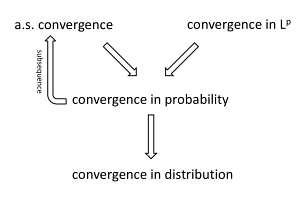
\includegraphics[width=4.28in]{images/basic_convergenceconnection} 

}

\caption{Connections between modes of convergences.}\label{fig:unnamed-chunk-130}
\end{figure}

\hypertarget{convergence-of-moments-uniform-integrability}{%
\section{Convergence of moments: 일양적분가능성(uniform integrability)}\label{convergence-of-moments-uniform-integrability}}

\(X_{n}\)이 점근적으로 \(\mathcal{N}(\mu_{n}, \sigma_{n}^{2})\)에 수렴한다는 문장을 생각해보자. 즉 이 얘기는 \((X_{n}-\mu_{n})/\sigma_{n} \stackrel{D}{\rightarrow} \mathcal{N}(0,1)\)이라는 말이다. 그러나 이것이 \(E(X_{n})=\mu_{n}\)이고 \(\text{var}(X_{n})=\sigma_{n}^{2}\)임을 의미하지는 않는다. 일반적으로 \(X_{n} \stackrel{D}{\rightarrow} X\)는 \(E(X_{n}) \rightarrow E(X)\)임을 의미하지 않는다.

\BeginKnitrBlock{example}[추정량은 무한대의 평균을 갖으나 확률변수의 극한은 유한한 평균을 갖는 예]
\protect\hypertarget{exm:unnamed-chunk-131}{}{\label{exm:unnamed-chunk-131} \iffalse (추정량은 무한대의 평균을 갖으나 확률변수의 극한은 유한한 평균을 갖는 예) \fi{} }\(\hat{p}_{n}\)이 iid 베르누이 확률변수 \(X_{1}, \ldots, X_{n}\)로부터 나온 표본비(sample proportion)라고 하자. 그러면 CLT에 의해 \(\hat{p}_{n}\)은 점근적으로 평균 \(p=E(X_{1})\)이고 분산 \(p(1-p)/n\)인 정규분포를 따른다. 델타 방법(delta method)에 의해 \(\text{ln}(\hat{p})\)는 점근적으로 평균 \(\ln(p)\), 분산 \((1-p)/(np)\)인 정규분포를 따름을 안다. 그러면
\[Z_{n} = \frac{\text{ln}(\hat{p}_{n})-\text{ln}(p)}{\sqrt{(1-p)/(np)}} \stackrel{D}{\rightarrow} Z \sim \mathcal{N}(0,1)\]
임을 안다. 그러나 모든 \(n\)에 대해 \(E\{\text{ln}(\hat{p}_{n}) \}=-\infty\)인데, 이는 \(\hat{p}_{n}\)은 0이 될 확률이 양수이기 때문이다. 그러므로 \(E(Z_{n})=-\infty\)이나, \(E(Z)=0\)이다.
\EndKnitrBlock{example}

(Skrohod 정리를 이용한 추가적 설명 필요, Essential of Probability Theory for Statisticians 193-194쪽)

\BeginKnitrBlock{definition}[일양적분가능]
\protect\hypertarget{def:unnamed-chunk-132}{}{\label{def:unnamed-chunk-132} \iffalse (일양적분가능) \fi{} }만약 각 \(\epsilon >0\)에 대해
\[E\{ |X_{n}| I(|X_{n}|>A)\}<\epsilon \forall n\]
을 만족하는 \(A\)가 존재한다면 이 확률변수의 수열 \(X_{n}\)을 \textbf{일양적분가능(uniformly integrable, UI)}이라고 부른다.
또는
\[\lim_{A\rightarrow\infty}\sup_{n}E\{ |X_{n}| I(|X_{n}|>A)\}=0\]
을 만족하는 것으로 정의하기도 한다.
\EndKnitrBlock{definition}

그렇다면 일양적분가능이 말하고자 하는 것은 무엇인가? \(|X_{n}| I(|X_{n}|>A)\)항부터 살펴보자. 이것은 \(A\)보다 작은 \(|X_{n}|\) 값은 0이 되도록 조절하는 것이다. 다음 그림을 참고하자.

\begin{figure}

{\centering 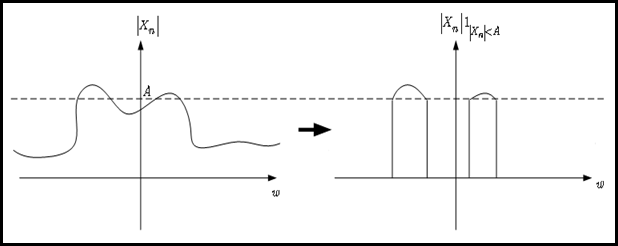
\includegraphics[width=8.58in]{images/basic_UI01} 

}

\caption{Case when function values bigger than A exist.}\label{fig:unnamed-chunk-133}
\end{figure}

다음은 \(E\{|X_{n}| I(|X_{n}|>A)\}\)에 초점을 맞춘다. 이것은 그림 \ref{fig:theoryUI01}의 그래프 아래 면적에 해당하는 것이다(물론 \(\omega \in [0,M]\)에서 균등한 확률 측도 \(dP(\omega)=\frac{1}{M}\)을 줬을 때의 이야기다). 이때 상한(\(\sup_{n}\))의 쓰임은 \(A\)가 고정되었을 때 가장 큰 면적을 반환하는 \(n\)을 찾는 것이다. 마지막으로 극한을 취함으로써(\(lim_{A\rightarrow\infty}\sup_{n}E\{ |X_{n}| I(|X_{n}|>A)\}\)) \(A\)가 점점 커졌을 때 상한이 어떻게 변하는지 관찰할 수 있다.

\begin{figure}

{\centering 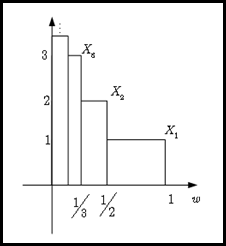
\includegraphics[width=3.14in]{images/basic_UI02} 

}

\caption{An example of sequence of random variables that is not uniformly integrable.}\label{fig:unnamed-chunk-134}
\end{figure}

위 확률변수의 수열은 일양적분가능하지 않다. \(A\)가 커짐에 따라 항상 \(E\{|X_{n}| I(|X_{n}|>A)\}=1\)을 만족하는 \(n\)이 존재한다. 즉 \(|X_{n}| I(|X_{n}|>A)=|X_{n}|\)인 \(n\)이 항상 존재하는 것이다. 따라서
\[\sup_{n}E\{ |X_{n}| I(|X_{n}|>A)\}=\sup_{n}E\{ |X_{n}|\}=\sup_{n}1=1.\]
이다.

\begin{figure}

{\centering 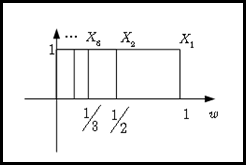
\includegraphics[width=3.42in]{images/basic_UI03} 

}

\caption{An example of sequence of random variables that is uniformly integrable.}\label{fig:unnamed-chunk-135}
\end{figure}

위 예들로부터 얻을 수 있는 직관적 사실들은 다음과 같다. 만약 \(X_{n}\)의 평균 면적이 \(n\)이 커짐에 따라 무한대로 발산하면 그 확률변수의 수열은 항상 일양적분가능하지 않을 것이다. 한편

\begin{itemize}
\item
  모든 유한한 수열을 항상 일양적분가능하다(왜냐하면 모든 고정된 \(n\)에 대해 \(P(X_{n}>A)\)는 \(A\)가 커짐에 따라 감소한다).
\item
  모든 유계(bounded)인 확률변수의 수열(반대로 유계가 아닌 경우를 생각해보면 \(n\)이 커짐에 따라 \(X_{n}\)은 어떤 확률로 점점 큰 값을 갖게 될 것이다)일양적분가능하다. 그러나 그 역은 성립하지 않는다.
\end{itemize}

마지막으로 유계가 아니나 일양적분가능한 확률변수의 수열의 예를 소개한다.

\begin{figure}
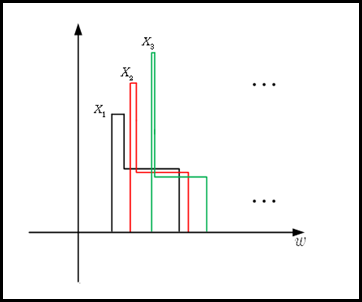
\includegraphics[width=5.03in]{images/basic_UI04} \caption{An example of sequence of random variables that is not bounded but uniformly integrable.}\label{fig:unnamed-chunk-136}
\end{figure}

\hypertarget{absolute-continuous}{%
\section{절대연속(absolute continuous)}\label{absolute-continuous}}

확률변수 \(X_{1}\), \(X_{2}\)가 있을 때 \(X_{1}\)이 \(X_{2}\)에 대해 \textbf{절대연속(absolute continuous)}하다는 것은(정확히 얘기하면 \(X_{1}\)의 분포가 \(X_{2}\)의 분포에 대해 절대연속이다) 적당한 집합 \(F\)에 대해 \(P(X_{2}\in F)=0\)이 \(P(X_{1}\in F)=0\)임을 내포하는 것과 동치이다.

\hypertarget{-law-of-large-numbers}{%
\section{대수의 법칙(law of large numbers)}\label{-law-of-large-numbers}}

\BeginKnitrBlock{proposition}[대수의 약법칙과 대수의 강법칙]
\protect\hypertarget{prp:unnamed-chunk-137}{}{\label{prp:unnamed-chunk-137} \iffalse (대수의 약법칙과 대수의 강법칙) \fi{} }\textbf{대수의 약법칙(weak law of large numbers, WLLN)}은 \(\bar{X}_{n}\)이 \(\mu\)에 확률수렴하는 것이고, \textbf{대수의 강법칙(strong law of large numbers, SLLN)}은 \(\bar{X}_{n}\)이 \(\mu\)에 거의 확실한 수렴을 하는 것이다.
\EndKnitrBlock{proposition}

\hypertarget{--convergence-of-functions-of-random-variables}{%
\section{확률변수들의 함수의 수렴(convergence of functions of random variables)}\label{--convergence-of-functions-of-random-variables}}

연속 사상 정리는 \citep{Gut2012}의 서술을 따른다.

\BeginKnitrBlock{theorem}[연속 사상 정리]
\protect\hypertarget{thm:contmappingthm}{}{\label{thm:contmappingthm} \iffalse (연속 사상 정리) \fi{} }\(X_{1}, X_{2},\ldots\)가 확률변수들이라고 하고 \(n\rightarrow \infty\)일 때 \(X_{n}\stackrel{d}{\rightarrow}\)라고 하자. 만약 (실수 값을 갖는) 함수 \(g\)가 존재해 이것이 연속이라면, \(n\rightarrow \infty\)일 때 \(g(X_{n})\stackrel{d}{\rightarrow}\)이다.
\EndKnitrBlock{theorem}

\hypertarget{markovchain}{%
\chapter{마르코프 체인}\label{markovchain}}

\hypertarget{-markov-chain}{%
\section{마르코프 체인(Markov chain)}\label{-markov-chain}}

\BeginKnitrBlock{definition}[마르코프 체인]
\protect\hypertarget{def:unnamed-chunk-138}{}{\label{def:unnamed-chunk-138} \iffalse (마르코프 체인) \fi{} }\textbf{마르코프 체인(Markov chain)}이란

\[P(X_{n+1}=X|X_{1}=x_{1}, X_{2}=x_{2}, \ldots , X_{n}=x_{n})=P(X_{n+1}=x|X_{n}=x_{n})\]

을 만족하는 확률변수들의 수열 \(X_{1},X_{2},\ldots\)를 일컫는다. 여기서\(x_{i}\)들은 countable set \(S\)에서 뽑힌 값들이며 \(S\)를 체인의 state space라고 부른다.
\EndKnitrBlock{definition}

\hypertarget{stoprocess}{%
\chapter{확률과정론}\label{stoprocess}}

참고할만한 책으로 \citep{Lindgren2012}가 있다.

\hypertarget{stochastic-process}{%
\section{확률과정이란?(stochastic process)}\label{stochastic-process}}

\citep{Lindgren2012}에 있는 그림이다.

\begin{figure}

{\centering 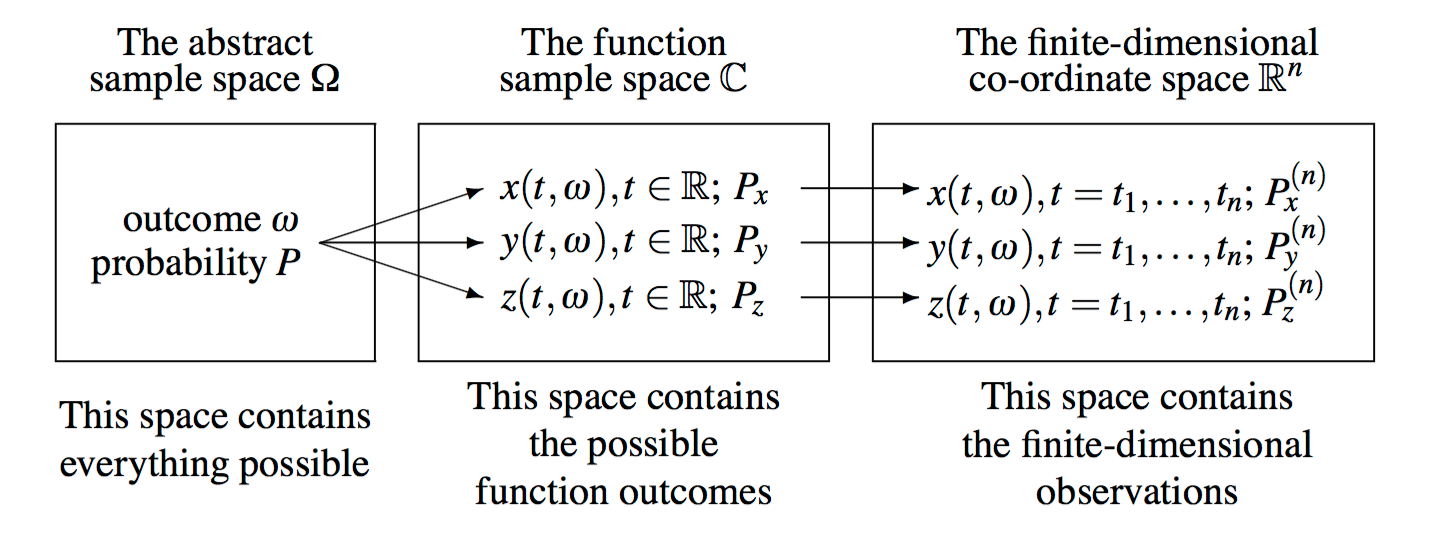
\includegraphics[width=19.94in]{images/basic_stprocess} 

}

\caption{Overview of the threee types of worlds in which our processes live.}\label{fig:unnamed-chunk-139}
\end{figure}

\textbf{확률과정(stochastic process)}란 확률공간에서 정의되는 확률변수들의 모임 \(\{ Z, t \in T\}\)라고 할 수 있다. 이 때 \(T=(-\infty, \infty)\) 등과 같이 연속된 구간의 형태를 갖는 경우를 \textbf{연속형 확률과정(continuous stochastic process)}, \(T=\{ 0, \pm 1, \pm 2 , \ldots\}\) 등과 같이 이산 구간일 경우는 \textbf{이산형 확률과정(discrete stochastic process)}라고 한다.

\hypertarget{stationary-stochastic-process}{%
\subsection{정상과정(stationary stochastic process)}\label{stationary-stochastic-process}}

정상과정은 \citep{Mikhail2014}에서 설명한 대로 시간의 전이(time shift)가 확률과정의 성질에 영향을 미치지 못하는 것을 의미한다. 수학적으로 얘기하면 어떤 \(s\in \mathbb{R}\)에 대해 확률과정 \(Y_{s}(t):= X(s+t)\)가 \(X\)와 equal in distirubtion임을 의미한다.

\hypertarget{-continuity-of-stochastic-process}{%
\section{확률과정에서의 연속성(continuity of stochastic process)}\label{-continuity-of-stochastic-process}}

\BeginKnitrBlock{definition}[연속표본경로]
\protect\hypertarget{def:unnamed-chunk-140}{}{\label{def:unnamed-chunk-140} \iffalse (연속표본경로) \fi{} }과정 \(X\)가 \(t_{0}\)에서 연속이라 함은
\[\text{For almost all }\omega, t \rightarrow t_{0} \text{ implies } X(t,\omega) \rightarrow X(t_{0},\omega)\]
를 의미한다. 과정 \(X\)가 연속이라 함은
\[\text{For almost all }\omega, X(\cdot, \omega) \text{ is a continuous function}\]
임을 의미한다.
\EndKnitrBlock{definition}

\BeginKnitrBlock{definition}[CADLAG (CAGLAD)]
\protect\hypertarget{def:unnamed-chunk-141}{}{\label{def:unnamed-chunk-141} \iffalse (CADLAG (CAGLAD)) \fi{} }Well-ordered set \(T\)에 있는 sample function \(x\)가 모든점에서 continuous from the right (left)하고 limited from the left (right)일 때 \textbf{CADLAG (CAGLAD)}이라고 한다. 즉, 모든 \(t_{0}\in T\)에서 \(t\downarrow t_{0}\)이 \(x(t) \rightarrow x(t_{0})\)를 의미하고 \(t\uparrow t_{0}\)일 때 \(\lim_{t\uparrow t_{0}} x(t)\)가 존재하나 꼭 \(x(t_{0})\)일 필요는 없는 상황임을 의미한다. 어떤 확률과정 \(X\)가 CADLAG임은 그것의 almost all sample path가 CADLAG임을 의미한다.
\EndKnitrBlock{definition}

\BeginKnitrBlock{definition}[확률과정의 version]
\protect\hypertarget{def:unnamed-chunk-142}{}{\label{def:unnamed-chunk-142} \iffalse (확률과정의 version) \fi{} }Common index set \(T\)를 갖는 두 개의 확률과정 \(X\)와 \(Y\)이 서로의 \textbf{version}이라 함은
\[\forall t \in T, \mathbb{P}(\omega: X(t,\omega)=Y(t,\omega))=1\]
임을 의미한다. 이러한 과정들을 \textbf{stochastically equivalent}라고도 부른다. 이는 임의의 시간대에서 \(X\)와 \(Y\)는 almost surely equal이라는 것이다.
\EndKnitrBlock{definition}

\BeginKnitrBlock{definition}[확률과정의 구분불가능성]
\protect\hypertarget{def:unnamed-chunk-143}{}{\label{def:unnamed-chunk-143} \iffalse (확률과정의 구분불가능성) \fi{} }두 개의 확률과정 \(X\)와 \(Y\)가 \textbf{구분불가능(indistinguishable)} 또는 \textbf{euqivalent up to evanescense}하다는 것은
\[\mathbb{P}(\omega: \forall t, X(t,\omega)=Y(t,\omega))=1\]
임을 의미한다. 쉽게 얘기하면 \(X\)와 \(Y\)의 표본 경로가 equal almost surely라는 것이다.
\EndKnitrBlock{definition}

구분불가능성을 갖는 확률과정은 서로의 version이 되나, 그 반대는 성립하지 않는다.

그렇다면 확률과정에서 왜 연속성이 이슈가 되는가? 우리는 sample path를 보통 연속인 함수로 제한하고 싶어한다. 더 나아가 미분가능할 정도로 부드러운 함수를 다루고자 하는 경우가 많다. 물론 이는 수학적인 편리함을 위해서이다.

\BeginKnitrBlock{proposition}
\protect\hypertarget{prp:unnamed-chunk-144}{}{\label{prp:unnamed-chunk-144} }\(X(t,\omega)\)를 실변수이며 연속 표본 경로를 갖는 연속 모수 과정이라고 하자. 그러면 모든 유한한 구간 \(I\)에 대해 \(M(\omega)=\equiv \sup_{t\in I}X(t,\omega)\)이고 \(m(\omega)\equiv \inf_{t\in I}X(t,\omega)\)는 가측 확률변수이다.
\EndKnitrBlock{proposition}

우리는 특정 시간에 관찰된 확률과정을 다룰 때 product \(\sigma\)-field를 보통 쓴다. Product \(\sigma\)-field는 countable question에 대해 답을 해 준다. 즉 어떤 measurable set \(A\)가 있으면 이 때 \(x(\cdot, \omega)\in A\)는 countably many indices \(t\)의 \(x(t,\omega)\) value들에 depend해야한다는 것이다. 이것은 모든 continuous sample path들의 class가 not product \(\sigma\)-field measurable이 될 수도 있다는 것을 의미하는데, 그 이유는 \(x(\cdot, \omega)\)가 \(t\)에서 연속이라는 것은 모든 수열 \(t_{n}\rightarrow t\)에 대해 \(x(t_{n},\omega)\rightarrow x(t,\omega)\)라는 것을 의미하면 이것은 uncountably many coordinates들의 함숫값들을 포함하는 것이기 때문이다. 더 나아가 differentiable function들의 class 또한 \(\sigma\)-field measurable이 아니다.

\hypertarget{--separable-random-functions}{%
\section{분리가능한 무작위 함수들(separable random functions)}\label{--separable-random-functions}}

\textbf{분리가능(separable)}한 무작위 함수들의 기본 아이디어는 contable, dense subset만 다룬다는 것이다.

\BeginKnitrBlock{definition}[분리가능 함수들(separable functions]
\protect\hypertarget{def:unnamed-chunk-145}{}{\label{def:unnamed-chunk-145} \iffalse (분리가능 함수들(separable functions) \fi{} }\(\Xi\)와 \(T\)가 metric space라고 하고, \(D\)를 \(T\)의 countable, dense subset이라고 하자. 그러면 함수 \(x: T\rightarrow \Xi\)가 \(\forall t\in T\)에 대해 수열 \(t_{i}\in D\)가 존재해 \(t_{i}\rightarrow t\) 그리고 \(x(t_{i})\rightarrow x(t)\)를 만족할 경우 함수 \(x\)를 \textbf{D-분리가능(D-separable)} 또는 D에 대해 분리가능하다고 한다.
\EndKnitrBlock{definition}

\BeginKnitrBlock{lemma}
\protect\hypertarget{lem:unnamed-chunk-146}{}{\label{lem:unnamed-chunk-146} }다음 조건들은 분리가능성의 충분조건이다.

\begin{enumerate}
\def\labelenumi{\arabic{enumi}.}
\item
  \(T\) is countable
\item
  \(T\) is continuous
\item
  \(T\) is well-ordered and \(x\) is right-continuous.
\end{enumerate}
\EndKnitrBlock{lemma}

\BeginKnitrBlock{proof}
\iffalse{} {Proof. } \fi{}1. \(T\) 자체를 separating set으로 잡으면 된다.

\begin{enumerate}
\def\labelenumi{\arabic{enumi}.}
\setcounter{enumi}{1}
\item
  어떤 countable dense set \(D\)를 잡는다. Dense 성질에 의해 모든 \(t\)에 대해 다음과 같은 수열 \(t_{i}\in D\)가 존재해 \(t_{i}\rightarrow t\)이다. 연속성에 의해 \(x(t_{i})\rightarrow t\)가 된다.
\item
  2와 마찬가지로 모든 coundtable dense \(D\)에 대해 \(t_{i}>t\)가 되도록인 채로 2와 같은 논리를 따라가면 된다.
\end{enumerate}
\EndKnitrBlock{proof}

\BeginKnitrBlock{definition}[분리가능 과정]
\protect\hypertarget{def:unnamed-chunk-148}{}{\label{def:unnamed-chunk-148} \iffalse (분리가능 과정) \fi{} }\(\Xi\)-valued process \(X\) on \(T\)가 \textbf{D에 대해 분리가능(separable with respect to D)}하다는 것은 \(D\)가 \(T\)의 countable, dense subset이고 다음과 같은 measure-zero set \(N\in\Omega\)가 존재해 모든 \(\omega \in N\)에 대해 \(X(\cdot, \omega)\)가 \(D\)-분리가능이라는 것이다. 즉 \(X(\cdot, \omega)\)가 almost surely \(D\)-separable이라는 것이다.
\EndKnitrBlock{definition}

\hypertarget{empirical-process}{%
\section{경험과정(empirical process)}\label{empirical-process}}

이 부분은 \citep{Jiang2010} 7장을 참고했다. 확률변수들은 관찰값(observation)들의 형태로 얻어지는데, 관찰된 확률변수들로 구성된 함수를 우리는 특별히 \textbf{통계적 함수(statistical function)}이라고 부른다. 통계적 함수는 실제로 얻을 수 있다는 점에서 많은 사람들이 그 성질에 대해 관심을 갖는다. 보통은 통계적 함수들 중 \textbf{경험과정(empriical process)}이라고 부르는 것에 집중을 하게 된다. \$X\_\{1\},X\_\{2\},\ldots \$가 분포함수 \(F\)를 갖는 i.i.d. 확률변수들의 수열이라고 하자. 그러면 \textbf{경험적 분포함수(empirical distribution function)}은 다음과 같이 정의된다.

\BeginKnitrBlock{definition}[경험적 분포함수]
\protect\hypertarget{def:unnamed-chunk-149}{}{\label{def:unnamed-chunk-149} \iffalse (경험적 분포함수) \fi{} }경험적 분포함수 \(F_{n}(x)\)는 다음과 같이 정의된다.

\begin{equation}
F_{n}(x)=\frac{1}{n}\sum_{i=1}^{n}1_{(X_{i}\leq x)}, -\infty < x < \infty.
\label{eq:empiricalDF}
\end{equation}
\EndKnitrBlock{definition}

식 \eqref{eq:empiricalDF}은 쉬워보이지만 이 식의 뜻을 쉽게 이해하기는 어렵다. 여기서 \(X_{i}\)들은 관찰값들이고 \(x\)는 함수값이다. \(X_{i}\)들의 실현(realization)에 대해 식 \eqref{eq:empiricalDF}은 계단함수를 정의한다. 그리고 \(X_{i}\)들이 무작위이므로 식 \eqref{eq:empiricalDF} 또한 무작위이다. 즉 \(X_{1},\ldots ,X_{n}\)들이 매 번 실현될 때마다 다른 함수를 얻게 된다.

대수의 약법칙에 의해 각 \(x\)에 대해 경험적 분포함수는 \(n\rightarrow\infty\)일 때 \(E\{1_{(X_{1}\leq X)}\}=P(X_{1}\leq x)=F(x)\)에 거의 확실한 수렴(converge a.s)을 한다. 실제로는 더 강한 결과가 성립한다. 이 거의 확실한 수렴은 \(n\rightarrow\infty\)일 때
\[\sup_{x}|F_{n}(x)-F(x)|\stackrel{\text{a.s.}}{\rightarrow}0\]
이므로 uniform하게 수렴한다. 그러면 우리는 경험적 분포함수에 대해서도 다음과 같은 centeralized되어있고 normalized version의 경험적 분포함수를 정의할 수 있다. 이를 \textbf{경험적 과정(empirical process)}라고 부른다.

\BeginKnitrBlock{definition}[경험적 과정]
\protect\hypertarget{def:unnamed-chunk-150}{}{\label{def:unnamed-chunk-150} \iffalse (경험적 과정) \fi{} }경험적 과정은 무작위 함수로 다음과 같이 정의된다.
\[\sqrt{n}\{ F_{n}(x) - F(x) \},\qquad{-\infty < x \infty.}\]
\EndKnitrBlock{definition}

\hypertarget{poisson-process}{%
\section{포아송과정(Poisson process)}\label{poisson-process}}

우리의 휴대전화로 오는 문제메시지는 하루종일 불규칙한 간격으로 온다. 고속도로에서의 사고들은 시간과 공간에 독립적으로 일어난다. 이러한 현상들은 연속 구간(보통 시간)에서의 발생 또는 도착 사건들을 모델링하는 데 사용되는 확률과정인 \textbf{포아송과정(Poisson process)}으로 잘 모델링할 수 있다.

\hypertarget{counting-process}{%
\subsection{셈과정(counting process)}\label{counting-process}}

포아송 과정은 \textbf{셈과정(counting process)}의 특별한 타입이다. 어떤 사건들의 흐름이 \(t=0\)에서 시작하는 시간대에서 무작위로 도착한다고 가정해보자. 이 때 \(t\)시간까지 도착한 사건의 숫자를 \(N_{t}\)라고 하자. 모든 \(t\geq 0\)에서 \(N_{t}\)는 확률변수다. 이런 확률변수들의 모임(collection) \((N_{t})_{t\geq 0}\)은 연속이며 정수값을 갖는 확률과정이고 이를 셈과정이라고 부른다. \(N_{t}\)는 \([0,t]\) 사이의 사건을 세기 때문에 \(t\)가 증가함에 따라 \(N_{t}\) 또한 증가한다.

\BeginKnitrBlock{definition}[셈과정]
\protect\hypertarget{def:unnamed-chunk-151}{}{\label{def:unnamed-chunk-151} \iffalse (셈과정) \fi{} }셈과정 \((N_{t})_{t\geq 0}\)은 음이 아니고 정수값을 갖는 확률변수들의 모임으로 \(0\leq s \leq t\)일 때 \(N_{s} \leq N_{t}\)이다.
\EndKnitrBlock{definition}

\begin{figure}

{\centering 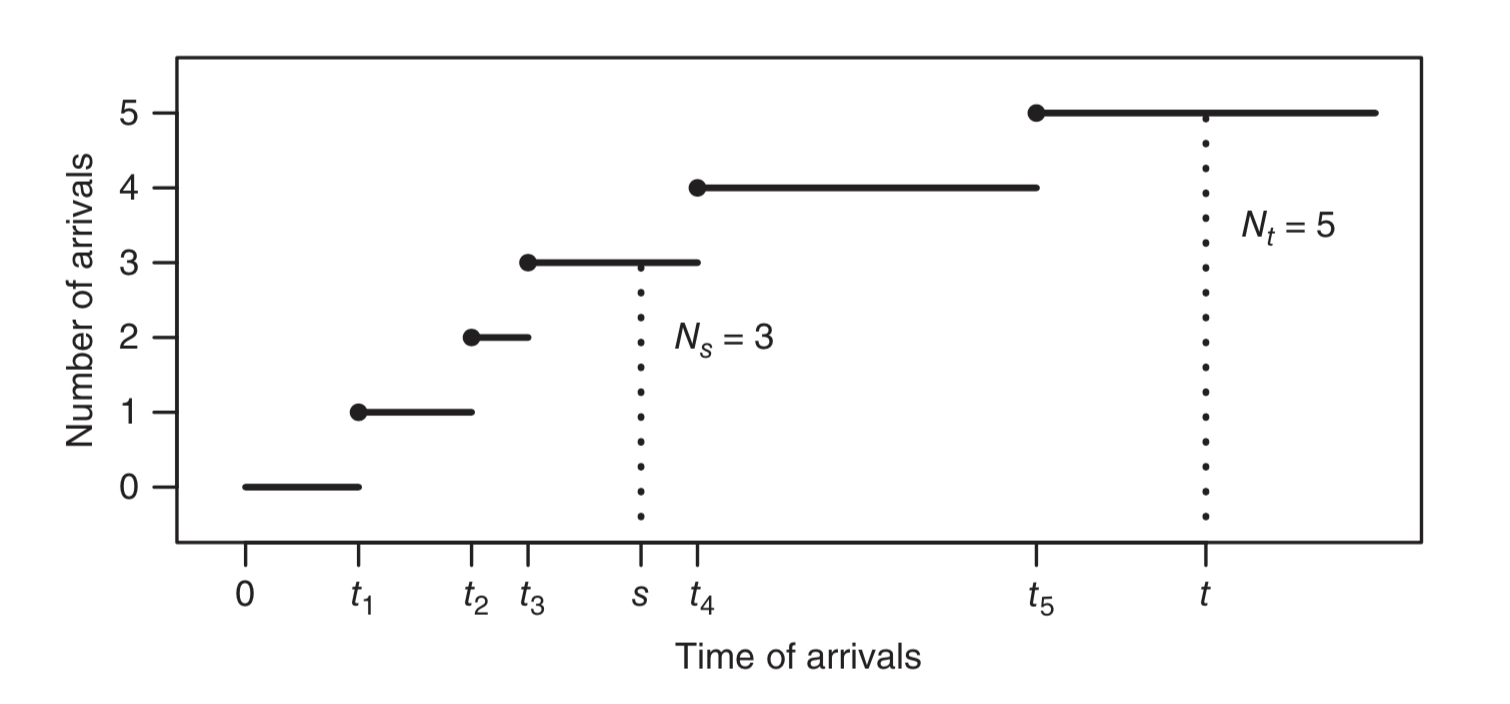
\includegraphics[width=20.97in]{images/stprocess_countingp} 

}

\caption{Example of counting process.}\label{fig:unnamed-chunk-152}
\end{figure}

확률변수들의 수열인 마르코프 체인과 다르게 셈과정은 연속인 시간 간격에서 indexed 되어 있으므로 셀 수 없는 모임이다.

\hypertarget{-definition-of-poisson-process}{%
\subsection{포아송과정의 정의(definition of Poisson process)}\label{-definition-of-poisson-process}}

\textbf{포아송과정(Poisson process)}을 정의하는 방법은 몇 가지가 있다.

\begin{enumerate}
\def\labelenumi{\arabic{enumi}.}
\item
  고정된 간격에서의 사건 숫자의 초점을 맞추는 방법
\item
  이떤 사건이 일어났을 때 사건들 사이의 시간에 초점을 맞추는 방법
\item
  무한소(infinitesimal, 모든 양수보다는 작지만 0보다 큰 상태) 간격에서의 개별 사건들의 확률적 행동에 초점을 맞추는 방법
\end{enumerate}

이에 따라 포아송과정의 정의도 세 가지가 있다.

\BeginKnitrBlock{definition}[포아송과정 (정의1)]
\protect\hypertarget{def:unnamed-chunk-153}{}{\label{def:unnamed-chunk-153} \iffalse (포아송과정 (정의1)) \fi{} }모수 \(\lambda\)를 갖는 포아송 과정\((N_{t})_{t\geq 0}\)은 다음 조건들을 만족하는 셈과정이다.

\begin{enumerate}
\def\labelenumi{\arabic{enumi}.}
\item
  \(N_{0}=0\).
\item
  모든 \(t>0\)에 대해 \(N_{t}\)는 모수 \(\lambda t\)를 갖는 포아송 분포를 따른다.
\item
  (정상 증분) 모든 \(s,t>0\)에 대해 \(N_{t+s}-N_{s}\)는 \(N_{t}\)와 같은 분포를 갖는다. 즉 다음을 만족한다.
\end{enumerate}

\[P(N_{t+s}-N_{s} = k) = P(N_{t} = k) = \frac{e^{-\lambda t}(\lambda t)^{k}}{k!},\qquad{k=0,1,\ldots}\]

\begin{enumerate}
\def\labelenumi{\arabic{enumi}.}
\setcounter{enumi}{3}
\tightlist
\item
  (독립 증분) \(0\leq q < r \leq s < t\)인 \(q,r,s,t\)에 대해 \(N_{t}-N_{s}\)와 \(N_{r}-N_{q}\)는 독립인 확률변수들이다.
\end{enumerate}
\EndKnitrBlock{definition}

\textbf{정상 증분(stationary increment)} 성질은 어떤 구간에서의 도착 숫자의 분포는 오직 구간의 길이에만 관련이 있다는 것이다. \textbf{독립 증분(independent increment)}성질은 disjoint intervals에서의 도착들의 숫자는 독립 확률 변수들이 된다는 것이다.

\hypertarget{--poisson-random-measures}{%
\subsection{포아송 무작위 측도들(Poisson random measures)}\label{--poisson-random-measures}}

다음 \href{http://www.math.wisc.edu/~kurtz/735/main735.pdf}{사이트}의 9장을 참고하였다. \citep{Mikhail2014} 또한 참고할만하다. \((E,\mathcal{E})\)를 가측공간이라고 하고, \(\nu\)를 \(\mathcal{E}\)에서의 \(\sigma\)-finite 측도라고 하자. \(\mathcal{N}(E)\)는 \(E\)에서의 counting measure의 collection이라고 하자, 즉 음이 아닌 정수값들의 측도이다. \(\xi\)는 만약 각각의 \(\omega \in \Omega\)에서 \(\xi(\omega, \cdot)\in\mathcal{N}(E)\)이고 각각의 \(A\in\mathcal{E}\)에서 \(\xi(A)\)가 \(\mathbb{N}\cup\{\infty\}\)의 값을 갖는 확률변수일 때 확률공간 \((\Omega, \mathcal{F}, P)\)에서의 \(\mathcal{N}(E)\)-확률변수다. 편의를 위해 \(\xi(\omega, A)\)대신 \(\xi(A)\)라고 쓰자.

\BeginKnitrBlock{definition}[포아송 무작위 측도]
\protect\hypertarget{def:unnamed-chunk-154}{}{\label{def:unnamed-chunk-154} \iffalse (포아송 무작위 측도) \fi{} }어떤 \(\mathcal{N}(E)\)-확률변수가

\begin{enumerate}
\def\labelenumi{\arabic{enumi}.}
\item
  각각의 \(A\in\mathcal{E}\)에 대해 \(\xi(A)\sim \text{Poisson}(\nu(A))\)이다.
\item
  만약 \(A_{1},A_{2},\ldots \in \mathcal{E}\)가 disjoint이면 \$\xi(A\_\{1\}), \xi(A\_\{2\}),\ldots \$는 독립인 확률변수이다.
\end{enumerate}

를 만족하면 \textbf{평균측도(mean measure)} \(\nu\)를 갖는 \textbf{포아송 무작위 측도(Poisson random measure)}이다.
\EndKnitrBlock{definition}

\(\nu\)는 \(\xi\)가 존재할 경우 \(\xi\)의 분포를 결정한다. 먼저 \(\nu\)가 유한하게 존재한다면 \(\nu\)가 \(\sigma\)-finite한 것으로 고려한다.

\BeginKnitrBlock{proposition}
\protect\hypertarget{prp:unnamed-chunk-155}{}{\label{prp:unnamed-chunk-155} }\(\nu\)가 \((E,\mathcal{E})\)에서의 측도이고 \(\nu(E)<\infty\)라고 하자. 그러면 평균측도 \(\nu\)를 갖는 포아송 무작위 측도가 존재한다.
\EndKnitrBlock{proposition}

평균측도를 다른 말로 intensity measure라고 부르기도 한다.

\hypertarget{--spatial-poisson-process}{%
\subsection{공간 포아송 과정(spatial Poisson process)}\label{--spatial-poisson-process}}

\citep{Dobrow2016}의 6.6절을 참고하였다. \textbf{공간 포아송 과정(spatial Poisson process)}란 사건 또는 점의 분포에 관한 모형으로, 2차원 이상 공간에서 다뤄지는 것이 특징이다. 이러한 과정의 예로 숲에서의 나무들의 장소에 대한 모형이나, 밤하늘 은하의 위치에 대한 모형 그리고 미국의 암 군집에 대한 모형 등을 들 수 있다.

\(d\geq 1\)이고 \(A\subset \mathbb{R}^{d}\)라고 할 때 \(N_{A}\)를 집합 \(A\)에 속하는 점들의 갯수로 정의하자. 그리고 \(|A|\)를 \(A\)의 size (즉 \(\mathbb{R}^{2}\)일 때에는 넓이, \(\mathbb{R}^{3}\)일 때에는 부피가 된다.)로 정의하자.

\BeginKnitrBlock{definition}[공간 포아송 과정]
\protect\hypertarget{def:unnamed-chunk-156}{}{\label{def:unnamed-chunk-156} \iffalse (공간 포아송 과정) \fi{} }확률변수들 \((N_{A})_{A\subseteq \mathbb{R}^{d}}\)가 다음의 두 조건

\begin{enumerate}
\def\labelenumi{\arabic{enumi}.}
\item
  각각의 유계집합 \(A\subseteq \mathbb{R}^{d}\)에 대해 \(N_{A}\)가 모수 \(\lambda |A|\)인 포아송 분포를 갖는다.
\item
  \(A\)와 \(B\)가 disjoint set일 때 \(N_{A}\), \(N_{B}\)는 독립인 확률변수들이 된다.
\end{enumerate}

을 만족하는 모수 \(\lambda\)를 갖는 공간 포아송 과정이라고 부른다.
\EndKnitrBlock{definition}

\BeginKnitrBlock{example}[공간 포아송 과정에서의 확률계산]
\protect\hypertarget{exm:unnamed-chunk-157}{}{\label{exm:unnamed-chunk-157} \iffalse (공간 포아송 과정에서의 확률계산) \fi{} }모수 \(\lambda=0.5\)인 공간 포아송 과정이 있다고 하자. \((3,4)\)를 중심으로 하고 반지름이 2인 디스크가 정확하게 5개의 점을 포함할 확률은 \(|C|=\pi r^{2}=4\pi\)를 이용하면
\[P(N_{C}=5)=\frac{e^{-\lambda |C|}(\lambda |C|)^{5}}{5!}=\frac{e^{-2\pi}(2\pi)^{5}}{5!}=0.152.\]
가 된다.
\EndKnitrBlock{example}

공간 과정에서 발생하는 균등분포는 1차원 포아송 과정에서 하는 일과 유사하다. 유계집합 \(A\subseteq \mathbb{R}^{d}\)이 주어졌을 때 \(A\)에 \(n\)개의 점이 있다고 조건을 달면 이 점들의 위치는 \(A\)에서 균등하게 분포되어 있어야 한다. 이러한 이유로 공간 포아송 과정을 때때로 \textbf{complete spatial randomness (CSR)} 모형이라고 부르기도 한다.

공간 포아송 과정은 공간상에서의 점의 분포를 모델링하는 일반적인 방법인 \textbf{점과정(point process)}의 특별한 경우이다. 때로는 주어진 포인트 패턴이 CSR과 얼마나 가까운지 측정하고 싶을 때도 있다. 그럴 때 사용할 수 있는 흔한 측도로 과정의 어떤 점과 그 점에서 가장 가까운 이웃과의 거리를 계산한 \textbf{최근접 거리(nearest neighbor distance)}가 있다.

모수가 \(\lambda\)인 \(\mathbb{R}^{2}\)에서의 공간 포아송 과정을 생각해보자. \(x\)를 plane에서의 고정된 점으로 둔다. \(D\)는 \(x\)의 최근접 거리라고 하자. 그러면 사건 \(\{ D > t\}\)는 \(x\)를 중심으로 하고 반지름이 \(t\)인 원 안에 다른 점이 하나도 없는 사건과 동치이다. 따라서 확률을
\[P(D>t)=P(N_{C_{x}}=0)=e^{-\lambda |C_{x}|} = e^{-\lambda \pi t^{2}}, \qquad{\text{for } t > 0}\]
과 같이 계산할 수 있다. 이것을 미분하면 최근접 거리에 대한 밀도함수를 얻을 수 있다.
\[f_{D}(t)=e^{-\lambda \pi t^{2}}2\lambda \pi t, \qquad{\text{for } t > 0.}\]
그리고 이것의 평균과 분산은 다음과 같다.
\[E(D) = \frac{1}{2\sqrt{\lambda}}, \text{Var}(D)=\frac{4-\pi}{4\pi\lambda}.\]

\hypertarget{----example-of-simulating-a-spatial-poisson-process}{%
\subsection{공간 포아송 과정 생성 예제(example of simulating a spatial Poisson process)}\label{----example-of-simulating-a-spatial-poisson-process}}

다음 R 예제는 \(\lambda=100\)인 포아송 과정을 영역 \([0,1]\times [0,1]\) 내에서 \((0.7,0.7)\)을 중심으로 하고 반지름이 \(r=0.2\)인 원 안에 들어가 있는 점의 갯수를 100,000번 반복 생성하여 계산해보고 기댓값과 비교해 보는 예제이다. 실제 기댓값은 \(\lambda |C|=100\pi (0.2)^{2}=12.567\)이다.

\begin{Shaded}
\begin{Highlighting}[]
\KeywordTok{library}\NormalTok{(plotrix)}
\CommentTok{# spatialPoisson.R}
\NormalTok{lambda <-}\StringTok{ }\DecValTok{100}
\NormalTok{squarearea <-}\StringTok{ }\DecValTok{1}
\NormalTok{trials <-}\StringTok{ }\DecValTok{100000}
\NormalTok{simlist <-}\StringTok{ }\KeywordTok{numeric}\NormalTok{(trials)}
\KeywordTok{par}\NormalTok{(}\DataTypeTok{mfrow=}\KeywordTok{c}\NormalTok{(}\DecValTok{2}\NormalTok{,}\DecValTok{2}\NormalTok{))}
\KeywordTok{par}\NormalTok{(}\DataTypeTok{mar=}\KeywordTok{c}\NormalTok{(}\FloatTok{5.1}\NormalTok{,}\FloatTok{4.1}\NormalTok{,}\FloatTok{4.1}\NormalTok{,}\FloatTok{2.1}\NormalTok{)}\OperatorTok{/}\DecValTok{4}\NormalTok{)}
\ControlFlowTok{for}\NormalTok{ (i }\ControlFlowTok{in} \DecValTok{1}\OperatorTok{:}\NormalTok{trials) \{}
\NormalTok{  N <-}\StringTok{ }\KeywordTok{rpois}\NormalTok{(}\DecValTok{1}\NormalTok{,lambda}\OperatorTok{*}\NormalTok{squarearea)}
\NormalTok{  xpoints <-}\StringTok{ }\KeywordTok{runif}\NormalTok{(N,}\DecValTok{0}\NormalTok{,}\DecValTok{1}\NormalTok{)}
\NormalTok{  ypoints <-}\StringTok{ }\KeywordTok{runif}\NormalTok{(N,}\DecValTok{0}\NormalTok{,}\DecValTok{1}\NormalTok{)}
\NormalTok{  ct <-}\StringTok{ }\KeywordTok{sum}\NormalTok{(((xpoints}\FloatTok{-0.7}\NormalTok{)}\OperatorTok{^}\DecValTok{2}\OperatorTok{+}\NormalTok{(ypoints}\FloatTok{-0.7}\NormalTok{)}\OperatorTok{^}\DecValTok{2}\NormalTok{)}\OperatorTok{<=}\FloatTok{0.2}\OperatorTok{^}\DecValTok{2}\NormalTok{)}
\NormalTok{  simlist[i] <-}\StringTok{ }\NormalTok{ct }
  \ControlFlowTok{if}\NormalTok{(i }\OperatorTok{<=}\DecValTok{4}\NormalTok{)\{}
    \KeywordTok{plot}\NormalTok{(xpoints,ypoints, }\DataTypeTok{xlim=}\KeywordTok{c}\NormalTok{(}\DecValTok{0}\NormalTok{,}\DecValTok{1}\NormalTok{), }\DataTypeTok{ylim=}\KeywordTok{c}\NormalTok{(}\DecValTok{0}\NormalTok{,}\DecValTok{1}\NormalTok{), }\DataTypeTok{xlab=}\StringTok{""}\NormalTok{, }\DataTypeTok{ylab=}\StringTok{""}\NormalTok{, }\DataTypeTok{main=}\StringTok{""}\NormalTok{,}\DataTypeTok{xaxt=}\StringTok{"n"}\NormalTok{,}\DataTypeTok{yaxt=}\StringTok{"n"}\NormalTok{)}
    \KeywordTok{draw.circle}\NormalTok{(}\DataTypeTok{x=}\FloatTok{0.7}\NormalTok{,}\DataTypeTok{y=}\FloatTok{0.7}\NormalTok{,}\DataTypeTok{radius=}\FloatTok{0.2}\NormalTok{,}\DataTypeTok{nv=}\DecValTok{100}\NormalTok{,}\DataTypeTok{border=}\StringTok{"black"}\NormalTok{,}\DataTypeTok{col=}\OtherTok{NA}\NormalTok{,}\DataTypeTok{lty=}\DecValTok{1}\NormalTok{,}\DataTypeTok{density=}\OtherTok{NULL}\NormalTok{,}
                \DataTypeTok{angle=}\DecValTok{45}\NormalTok{,}\DataTypeTok{lwd=}\DecValTok{1}\NormalTok{)}
\NormalTok{  \}}
\NormalTok{\} }\CommentTok{# number of points in circle}
\end{Highlighting}
\end{Shaded}

\begin{figure}

{\centering 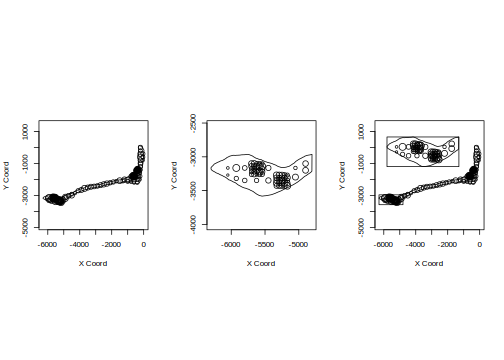
\includegraphics{book_files/figure-latex/unnamed-chunk-158-1} 

}

\caption{Samples of a spatial Poisson process.}\label{fig:unnamed-chunk-158}
\end{figure}

\begin{Shaded}
\begin{Highlighting}[]
\KeywordTok{mean}\NormalTok{(simlist)}
\end{Highlighting}
\end{Shaded}

\begin{verbatim}
> [1] 12.57759
\end{verbatim}

\begin{Shaded}
\begin{Highlighting}[]
\KeywordTok{var}\NormalTok{(simlist)}
\end{Highlighting}
\end{Shaded}

\begin{verbatim}
> [1] 12.56107
\end{verbatim}

\begin{Shaded}
\begin{Highlighting}[]
\CommentTok{# Compare with theoretical mean and variance}
\NormalTok{lambda}\OperatorTok{*}\NormalTok{pi}\OperatorTok{*}\NormalTok{(}\FloatTok{0.2}\NormalTok{)}\OperatorTok{^}\DecValTok{2}
\end{Highlighting}
\end{Shaded}

\begin{verbatim}
> [1] 12.56637
\end{verbatim}

\hypertarget{--nonhomogeneous-poisson-process}{%
\subsection{비동질적 포아송 과정(nonhomogeneous Poisson process)}\label{--nonhomogeneous-poisson-process}}

포아송 과정에서, 도착은 시간과 독립이다. 그러나 많은 응용에서 이는 비현실적인 가정이다. 대학 식당의 점심시간을 생각해보자. 문을 오전 11시에 연다고 했을 때 학생들의 도착을 정오까지 점점 증가하다가 상수를 이루다 문을 닫는 시간인 낮 3시까지 감소하게 될 것이다. 이러한 행동들은 율(rate)가 \(\lambda=\lambda(t)\)인 \textbf{비동질적 포아송 과정(nonhomogeneous Poisson process)}으로 모델링할 수 있다. 이러한 율 함수를 \textbf{강도함수(intensity function)}라고 부른다.

\BeginKnitrBlock{definition}[비동질적 포아송 과정]
\protect\hypertarget{def:unnamed-chunk-159}{}{\label{def:unnamed-chunk-159} \iffalse (비동질적 포아송 과정) \fi{} }셈과정(counting process) \((N_{t})_{t\geq 0}\)은 다음 조건들을 만족할 때

\begin{enumerate}
\def\labelenumi{\arabic{enumi}.}
\item
  \(N_{0}=0\).
\item
  모든 \(t>0\)에 대해 \(N_{t}\)는 평균이 \(E(N_{t})=\int_{0}^{t}\lambda(x)dx\)인 포아송 분포를 갖는다.
\item
  \(0\leq q < r \leq s < t\)인 \(q,r,s,t\)에 대해 \(N_{r}-N_{q}\) \(N_{t}-N_{s}\)가 독립인 확률변수다.
\end{enumerate}

강도함수가 \(\lambda(t)\)인 비동질적 포아송과정이다.
\EndKnitrBlock{definition}

비동질적 포아송 과정인 독립 증분을 갖으나 정상 증분(stationary increment)을 가질 필요는 없다. 이는 \(0<s<t\)일때 \(N_{t}-N_{s}\)는 모수 \(\int_{s}^{t}\lambda(x)dx\)를 갖는 포아송 분포를 갖음으로부터 알 수 있다.

\hypertarget{---theory-of-spatial-poisson-process}{%
\subsection{공간 포아송 과정 이론(theory of spatial Poisson process)}\label{---theory-of-spatial-poisson-process}}

이 절은 Rasmussen의 2011년 강의노트를 따른다.

\hypertarget{-infinitely-divisible-distribution}{%
\section{무한분해가능 분포(infinitely divisible distribution)}\label{-infinitely-divisible-distribution}}

\citep{Gut2012}의 9.4에 오는 내용이다.

\BeginKnitrBlock{definition}[무한분해가능 분포]
\protect\hypertarget{def:unnamed-chunk-160}{}{\label{def:unnamed-chunk-160} \iffalse (무한분해가능 분포) \fi{} }어떤 확률변수 \(X\)의 각 \(n\)에 대해 독립이며 같은 분포를 따르는 확률변수들 \(X_{n,k},1\leq k \leq n\)이 존재해
\[X\stackrel{d}{=}\sum_{k=1}^{n} X_{n,k}, \qquad{\forall n}\]
이면 이 확률변수 \(X\)를 \textbf{무한분해가능(infinitely divisible)}이라고 부른다.

동치조건으로 특성함수(characteristic function)으로
\[\phi_{X}(t) = (\phi_{X_{n,1}}(t)), \qquad{\forall n}\]
인 경우 무한분해가능하다.
\EndKnitrBlock{definition}

\hypertarget{self-similar-process}{%
\section{자기유사과정(self-similar process)}\label{self-similar-process}}

\citep{Beran2013}에 따르면 long memory를 분석하는 고전적인 방법 중에 하나로 dependence과 self-similarity 사이의 관계에 기반한 방법이 있다.

\BeginKnitrBlock{definition}[자기유사과정]
\protect\hypertarget{def:unnamed-chunk-161}{}{\label{def:unnamed-chunk-161} \iffalse (자기유사과정) \fi{} }확률과정 \(Y(u)\) \((u\in \mathbb{R})\)은 모든 \(c>0\)에 대해
\[(Y(cu),u\in\mathbb{R})\stackrel{d}{=}(c^{H}Y(u), u\in\mathbb{R})\]
인 경우 이 확률과정을 \textbf{자기유사모수(self-similar parameter)} \(H\)를 갖는 \textbf{자기유사과정(self-similar process)}이라고 부른다.
\EndKnitrBlock{definition}

\hypertarget{brownian-motion}{%
\section{브라운운동(Brownian motion)}\label{brownian-motion}}

\citep{Mikhail2014}에 따르면 브라운운동은 확률과정으로, 200여년 전인 1827년 로버트 브라운(Robert Brown)이라는 식물학자에 의해 발견된 물리학적 현상이다. 1905년에 알버트 아인슈타인(Albert Einstein)은 위치 \(x\)와 시간 \(t\)에서의 분자를 다음과 같은 편미분 열 방정식(partial differential heat equation)으로 보일 수 있음을 보였다.
\[\frac{\partial}{\partial f}f(x,t) = \frac{1}{2}\frac{\partial^2}{\partial x^2}f(x,t).\]
이 때 \(f(x,t)\)는 위치 \(x\)와 시간 \(t\)에서의 밀도(단위 부피당 분자의 갯수)를 의미한다. 위의 등식을 풀면
\[f(x,t) = \frac{1}{\sqrt{2\pi t}}e^{-\frac{x^2}{2t}}\]
을 얻게 되는데 이것은 평균이 0, 분산이 \(t\)인 정규분포의 확률밀도함수다.

함수자료분석에서 다루는 가우스 무작위 함수(Gauss random function)들 중 가장 자주 일어나는 형태는

\begin{enumerate}
\def\labelenumi{\arabic{enumi}.}
\item
  \textbf{브라운운동(Brownian motion)}: 다른 말로 \textbf{위너과정(Wiener process)}이라고도 부른다. \citep{Kokoszka2017}의 11.4절, \citep{Mikhail2014}
\item
  \textbf{브라운 다리(Brownian bridge)}
\end{enumerate}

이다.

\BeginKnitrBlock{definition}[저차원에서의 브라운운동]
\protect\hypertarget{def:unnamed-chunk-162}{}{\label{def:unnamed-chunk-162} \iffalse (저차원에서의 브라운운동) \fi{} }실수값을 갖는 확률과정 \(\{ B_{t} : t\geq 0\}\)이 다음 조건들을 만족할 때

\begin{enumerate}
\def\labelenumi{\arabic{enumi}.}
\item
  \(B_{0}=x\)
\item
  (정규 분포) 모든 \(t >0\)에 대해 \(B_{t}\)는 평균이 0이고 분산이 \(t\)인 정규분포를 갖는다.
\item
  (Stationary increments) 모든 \(h,t>0\)에 대해 \(B_{t+h}-B_{h}\)가 \(B_{t}\)와 같은 확률변수를 갖는다. 즉
  \[B_{t+h}-B_{h} \sim \mathcal{N}(0,h)\]
  이다. 다른 표현으로는 모든 \(-\infty < z < \infty\)인 \(z\)에 대해
  \[P(B_{t+h} - B_{t} \leq z ) = P(B_{t}\leq z)  = \int_{-\infty}^{z}\frac{1}{\sqrt{2\pi t}}e^{-\frac{x^2}{2t}} dx\]
  가 되는 것이다.
\item
  (Independent increments) 모든 \(0 \leq q < r \leq s < t\)인 \(q,r,s,t\)에 대해 \(B_{t}-B_{s}\)와 \(B_{r}-B_{q}\)는 독립인 확률변수다.
\item
  (Continuous paths) 함수 \(t\rightarrow B_{t}\)는 확률 1로 연속이다.
\end{enumerate}

\(x\in\mathbb{R}\)에서 시작하는 (선형) \textbf{브라운운동(Brownian motion)}이라고 한다. 특별히 \(x=0\)일 때 \(\{ B_{t}: t\geq 0\}\)을 정규 브라운운동(standard Brownian motion)이라고 부른다.
\EndKnitrBlock{definition}

브라운운동의 정의는 나중에 공간과정에도 잠시 나올 것이다.

\begin{figure}

{\centering 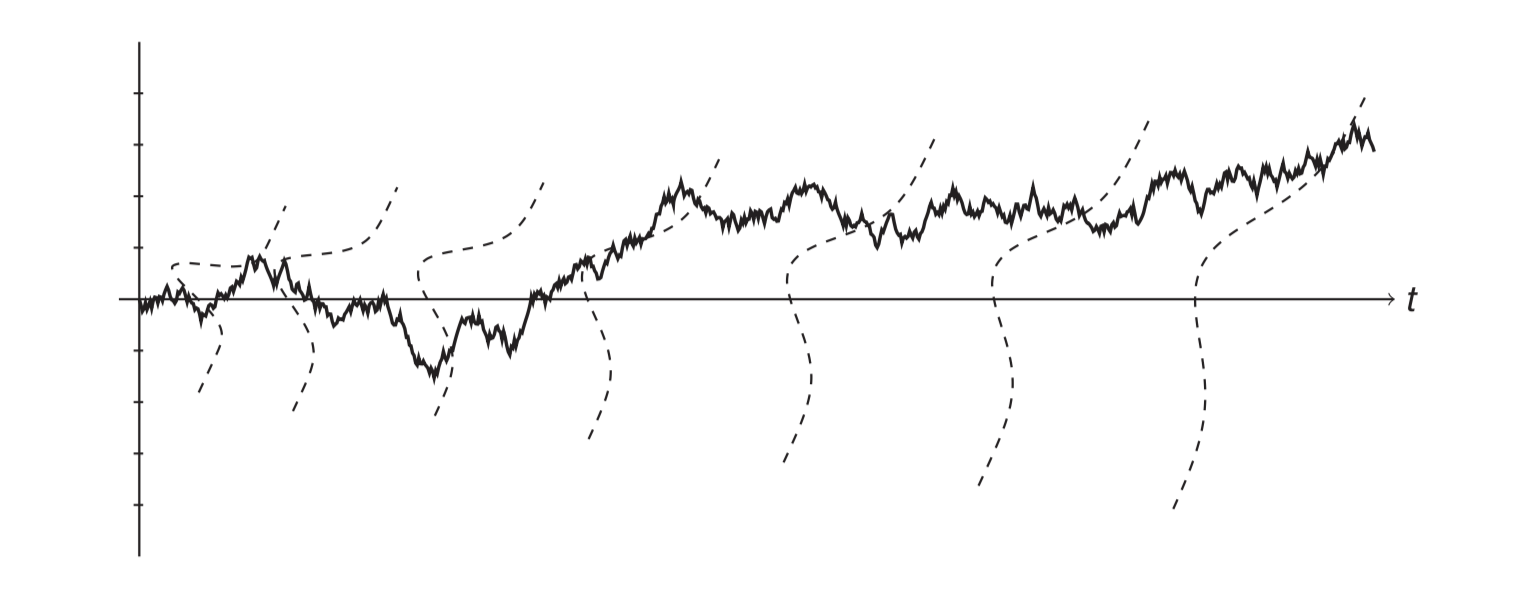
\includegraphics[width=21.33in]{images/stprocess_contpath} 

}

\caption{Browninan motion path.}\label{fig:unnamed-chunk-163}
\end{figure}

\BeginKnitrBlock{example}[브라운운동들의 합의 분포]
\protect\hypertarget{exm:unnamed-chunk-164}{}{\label{exm:unnamed-chunk-164} \iffalse (브라운운동들의 합의 분포) \fi{} }\(0<s<t\)일 때 \(B_{s} + B_{t}\)의 분포를 찾아보자. 우리는 \(B_{s}+B_{t} = 2B_{s} + (B_{t} - B_{s})\)로 놓을 수 있다. Independent increments에 의해 \(B_{s}\)와 \(B_{t}-B_{s}\)는 독립인 확률변수이고 따라서 \(2B_{s}\)와 \(B_{t}-B_{s}\)는 독립이다. 정규확률변수의 합 또한 정규이므로 \(B_{s}+B_{t}\) 또한 평균이 \(E(B_{s}+B_{t})=E(B_{s})+E(B_{t})=0\)이고 분산

\[
\begin{align*}
\text{Var}(B_{s}+B_{t}) &= \text{Var}(2B_{s} + (B_{t} - B_{s}))\\
&= \text{Var}(2B_{s}) + \text{Var}(B_{t} - B_{s})\\
&= 4\text{Var}(B_{s}) + Var(B_{t-s})\\
&= 4s + (t-s) = 3s+t
\end{align*}
\]

을 갖는 정규분포를 따른다.따라서 \(B_{s} + B_{t} \sim \mathcal{N}(0,3s+t)\)이다.
\EndKnitrBlock{example}

\BeginKnitrBlock{example}[브라운운동을 통한 입자의 위치 확률 계산]
\protect\hypertarget{exm:unnamed-chunk-165}{}{\label{exm:unnamed-chunk-165} \iffalse (브라운운동을 통한 입자의 위치 확률 계산) \fi{} }어떤 입차의 위치를 정규 브라운운동으로 모델링한다고 하자. 만약 \(t=2\)일 때 입자가 1에 위치하고 있을 경우 \(t=5\)일 때 3보다 작거나 같은 지점에 위치할 확률을 구해보자.

\[
\begin{align*}
P(B_{5} \leq 3| B_{2} = 1) &= P(B_{5}-B_{2} \leq 3-B_{2} | B_{2}=1)\\
&= P(B_{5}-B_{2} \leq 2 | B_{2} = 1)\\
&= P(B_{5} - B_{2} \leq 2)\\
&= P(B_{3} \leq 2) = 0.876.
\end{align*}
\]

이 때 세 번째 등식은 \(B_{5}-B{2}\)와 \(B_{2}\)가 독립임을 이용한 것이다.
\EndKnitrBlock{example}

\BeginKnitrBlock{example}[브라운운동의 공분산]
\protect\hypertarget{exm:unnamed-chunk-166}{}{\label{exm:unnamed-chunk-166} \iffalse (브라운운동의 공분산) \fi{} }\(B_{s}\)와 \(B_{t}\)의 공분산을 구해보자. \(\text{Cov}(B_{s},B_{t}) = E(B_{s}B_{t})-E(B_{s}B_{t}) = E(B_{s}B_{t})\)이므로 \(E(B_{s}B_{t})\)만 구하면 된다. \(s<t\)일 때 \(B_{t}=(B_{t}-B_{s})+B_{s}\)이며 따라서

\[
\begin{align*}
E(B_{s}B_{t}) &= E(B_{s}(B_{t}-B_{s}+B_{s}))\\
&= E(B_{s}(B_{t}-B_{s}))+E(B_{s}^{2})\\
&=E(B_{s})E(B_{t}-B_{s}) + E(B_{s}^2)\\
&= 0 + \text{Var}(B_{s}) = s
\end{align*}
\]

를 얻는다. 따라서 \(\text{Cov}(B_{s},B_{t})=s\)다. 만약 반대로 \(t<s\)라면 \(\text{Cov}(B_{s},B_{t})=t\)일 것이다. 따라서 \(\text{Cov}(B_{s} ,B_{t})=\min\{s,t\}\)가 된다.
\EndKnitrBlock{example}

\begin{Shaded}
\begin{Highlighting}[]
\CommentTok{# bm.R}
\NormalTok{n <-}\StringTok{ }\DecValTok{1000}
\NormalTok{t <-}\StringTok{ }\DecValTok{1}
\NormalTok{bm <-}\StringTok{ }\KeywordTok{c}\NormalTok{(}\DecValTok{0}\NormalTok{, }\KeywordTok{cumsum}\NormalTok{(}\KeywordTok{rnorm}\NormalTok{(n,}\DecValTok{0}\NormalTok{,}\KeywordTok{sqrt}\NormalTok{(t}\OperatorTok{/}\NormalTok{n))))}
\NormalTok{steps <-}\StringTok{ }\KeywordTok{seq}\NormalTok{(}\DecValTok{0}\NormalTok{,t,}\DataTypeTok{length=}\NormalTok{n}\OperatorTok{+}\DecValTok{1}\NormalTok{)}
\KeywordTok{plot}\NormalTok{(steps,bm,}\DataTypeTok{type=}\StringTok{"l"}\NormalTok{)}
\end{Highlighting}
\end{Shaded}

\begin{figure}

{\centering 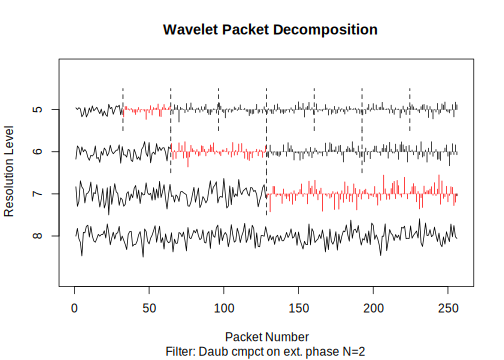
\includegraphics{book_files/figure-latex/unnamed-chunk-167-1} 

}

\caption{Simulating Brownian Motion.}\label{fig:unnamed-chunk-167}
\end{figure}

\hypertarget{-fractional-brownian-motion}{%
\subsection{분수 브라운운동(fractional Brownian motion)}\label{-fractional-brownian-motion}}

\textbf{분수 브라운운동(fractional Brownian motion)}이란 fractional derivative (또는 fractional integral) of Brownian motion을 일컫는 말이다. \citep{Mallat2008}에 따르면 분수 브라운운동은 통계적으로 자기유사성을 갖는 가우스 과정으로 자연현상을 모델링할 때 많이 쓰인다고 한다. 그 과정은 비정상성을 띄나 power decay를 갖는 power spectrum을 정의할 수 있다.

\hypertarget{gaussian-stochastic-process}{%
\section{가우스과정(Gaussian stochastic process)}\label{gaussian-stochastic-process}}

\textbf{가우스과정(Gaussian process)}는 연속시간 확률과정으로 가우스 분포를 무한차원으로 확장한 것이다. 또는 다변량 정규분포를 확륙과정으로 확장한 것이라고 보면 된다.

\BeginKnitrBlock{definition}[가우스과정]
\protect\hypertarget{def:unnamed-chunk-168}{}{\label{def:unnamed-chunk-168} \iffalse (가우스과정) \fi{} }\textbf{가우스과정(Gaussian process)} \(\{X_{t}\}_{t\geq 0}\)는 연속시간 확률과정으로 모든 \(n=1,2,\ldots\), \(0\leq t_{1} < \ldots < t_{n}\)에 대해 확률변수들 \(X_{t_{1}}, \ldots, X_{t_{n}}\)이 다변량 정규분포를 갖는 확률과정이다. 가우스과정은 그것의 평균함수 \(E(X_{t}), t\geq 0\)과 공분산함수 \(\text{Cov}(X_{s},X_{t}), s,t \geq 0\)에 의해 완벽하게 정의된다.
\EndKnitrBlock{definition}

정규 브라운운동은 가우스과정이다. 다음은 언제 가우스과정이 정규 브라운운동이 될 수 있는지에 대해 보여준다.

\BeginKnitrBlock{theorem}[정규 브라운운동과 가우스과정 사이의 관계]
\protect\hypertarget{thm:unnamed-chunk-169}{}{\label{thm:unnamed-chunk-169} \iffalse (정규 브라운운동과 가우스과정 사이의 관계) \fi{} }어떤 확률과정 \(\{ B_{t}\}_{t\geq 0}\)이 정규 브라운운동인 것은 다음을 만족하는 가우스과정임과 필요충분(동치)이다.

\begin{enumerate}
\def\labelenumi{\arabic{enumi}.}
\item
  \(B_{0}=0\).
\item
  (평균함수) \(E(B_{t})=0, \forall t\).
\item
  (공분산함수) \(\text{Cov}(B_{s},B_{t})=\min\{s,t\}, \forall s,t\).
\item
  (연속경로) 함수 \(t\rightarrow B_{t}\)가 확률 1로 연속.
\end{enumerate}
\EndKnitrBlock{theorem}

\hypertarget{martingale}{%
\section{마팅게일(martingale)}\label{martingale}}

\textbf{마팅게일(martingale)}은 평균 0을 갖는 독립인 확률변수들의 합의 일반화이다. 마팅게일은 확률과 통계에서 중요한 역할을 하며, 과거의 모든 정보를 알고 있다면 미래의 기댓값이 현재 값과 동일한 과정이다. 마팅게일이라는 말은 원래 도박에서 유래하였다고 한다. 마팅게일을 정의할 때는 조건부 기댓값이 중요한 역할을 한다.

\BeginKnitrBlock{definition}[마팅게일]
\protect\hypertarget{def:unnamed-chunk-170}{}{\label{def:unnamed-chunk-170} \iffalse (마팅게일) \fi{} }확률과정 \(\{X_{n}\}\)가

\begin{enumerate}
\def\labelenumi{\arabic{enumi}.}
\item
  \(E |X_{n}| < \infty\)
\item
  \(X_{n}\) is adpated to \(\mathcal{F}_{n}\). (즉 모든 \(n\)에 대해 \(X_{n}\in\mathcal{F}_{n}\))
\item
  \(E(X_{n+1}|\mathcal{F}_{n})=X_{n}, \text{ for all } n\)
\end{enumerate}

을 만족할 때, 이 확률과정을 filtration \(\mathcal{F}_{n}\)에 대한 \textbf{마팅게일(martingale)}이라 부른다.
\EndKnitrBlock{definition}

\hypertarget{bigOsmallo}{%
\chapter{Big O 와 small o}\label{bigOsmallo}}

Large-sample technique의 장점 중 하나는 중요한 부분과 minor한 부분으로 나눌 수 있게 한다는 점이다. 다음은 order에 관한 \citep{Jiang2010}의 예제이다.

\BeginKnitrBlock{example}[Order 고려의 중요성 (1)]
\protect\hypertarget{exm:unnamed-chunk-171}{}{\label{exm:unnamed-chunk-171} \iffalse (Order 고려의 중요성 (1)) \fi{} }\(X_{1},\ldots , X_{n}\)이 i.i.d.로 얻어진 표본들이며 \(\mu=E(X_{1})\neq 0\)이라고 하자. 그러면 우리는 \(\sum_{i=1}^{n}X_{i}\)로 기댓값들의 합 \(E(\sum_{i=1}^{n}X_{i})=n\mu\)를 대체할 수 있다. 이것은 \(\sum_{i=1}^{n}X_{i}-n\mu\)가 order \(O(\sqrt{n})\)으로, \(\sum_{i=1}^{n}X_{i}\)의 order보다 낮기 때문이다. 그러나 이러한 technique은 우리가 \((\sum_{i=1}^{n}X_{i})^{2}\)를 고려할 때에는 완벽하게 실패한다. 예를 들면 \(X_{i}\sim \mathcal{N}(0,1)\)이라고 하자. 그러면 \(E(\sum_{i=1}^{n}X_{i})^{2}=n\)이다. 그러나, \(\sum_{i=1}^{n}X_{i}\sim\mathcal{N}(0,n)\)이고 \((\sum_{i=1}^{n}X_{i})^{2}=n\{\frac{1}{\sqrt{n}}\sum_{i=1}^{n}X_{i} \}^{2} \sim n\chi_{1}^{2}\)이므로, \((\sum_{i=1}^{n}X_{i})^{2}-E(\sum_{i=1}^{n}X_{i})^{2}=n(\chi_{1}^{2}-1)\)이고 이는 \(E(\sum_{i=1}^{n}X_{i})^{2}\)와 같은 order이다. 따라서 \((\sum_{i=1}^{n}X_{i})^{2}\)은 \(E(\sum_{i=1}^{n}X_{i})^{2}\)의 좋은 근사가 아니다.
\EndKnitrBlock{example}

\BeginKnitrBlock{example}[Order 고려의 중요성 (2)]
\protect\hypertarget{exm:unnamed-chunk-172}{}{\label{exm:unnamed-chunk-172} \iffalse (Order 고려의 중요성 (2)) \fi{} }앞선 예제를 다시 생각해보자. \(X_{1},\ldots , X_{n}\)이 i.i.d.로 얻어진 표본들이며 \(\mu=E(X_{1})\neq 0\)이라고 하자. 이때 우리가 \(\sum_{i=1}^{n}X_{i}\)로 기댓값들의 합 \(E(\sum_{i=1}^{n}X_{i})=n\mu\)를 대체할 수 있는 이유는 쉽게 생각하면, WLLN으로 인해 \(\bar{X}=\frac{\sum_{i=1}^{n}X_{i}}{n}\)이 \(\mu\)의 consistent estimator이기 때문이다. 따라서 \(E(\sum_{i=1}^{n}X_{i})=n\mu\)를 \(n\bar{X}=\sum_{i=1}^{n}X_{i}\)로 추정하는 것은 일리가 있다.

이 방법을 다른 관점에서 바라보자. 만약 \(X_{i}\)들이 not i.i.d.일 경우, 어떻게 일반화 할 것이다. 우리는 앞 기대값을 다음과 같이 쓸 수 있다.
\[
\begin{eqnarray}
E(\sum_{i=1}^{n}X_{i})&=&\sum_{i=1}^{n}X_{i}-\{ \sum_{i=1}^{n}X_{i}-E(\sum_{i=1}^{n}X_{i})\}\\
&=&I_{1}-I_{2}.
\end{eqnarray}
\]

이제 \(I_{1}\)과 \(I_{2}\)의 order를 비교해보자. \(X_{i}\)들이 유한한 분산 \(\sigma, 0<\sigma^{2}<\infty\)을 갖는다고 하자. 그러면 \(I_{1}\)의 order는 \(O_{n}\)이고 \(I_{2}\)의 order는 \(O(\sqrt{n})\)이다. 좀 더 자세히 보자면 WLLN으로 인해 \(\frac{\sum_{i=1}^{n}X_{i}}{n}\stackrel{p}{\rightarrow}\mu\neq 0\)이고, 이는 \(I_{1}=O(n)\)임을 의미한다. 한편, \(E(I_{2}^{2})=n\sigma^{2}\)임을 보일 수 있고 이는 \(E(\frac{I_{2}}{\sqrt{n}})^{2}=\sigma^{2}\)임을 의미한다. 이것은 \(\frac{I_{2}}{\sqrt{n}}\)이 \(L^{2}\)에서 유계(bounded)임을 의미한다. 따라서, \(\frac{I_{2}}{\sqrt{n}}=O(1)\)이고 이는 \(I_{2}=O(\sqrt{n})\)으로 쓸 수 있다. (여기서 \(I_{1}, I_{2}\)는 모두 확률변수이다.) Order로 미루어 볼 때 \(E(\sum_{i=1}^{n}X_{i})\)를 \(I_{1}\)으로 근사하는 것이 main part를 잡아준다는 점에서 reaseonable하다는 것을 알 수 있다.

한편, 두 번째 케이스로 넘어가서, \(E(\sum_{i=1}^{2}X_{i})^{2}\)을 추정하는 문제를 생각해보자. 간단히 하기 위해 \(\mu=0\)이라고 가정한다. 그러면
\[
\begin{eqnarray}
E(\sum_{i=1}^{n}X_{i})^{2}&=&(\sum_{i=1}^{n}X_{i})^{2}-\{ (\sum_{i=1}^{n}X_{i})^{2}-E(\sum_{i=1}^{n}X_{i})^{2}\}\\
&=&I_{1}-I_{2}.
\end{eqnarray}
\]

으로 쓸 수 있다. 우리는 여기서 또 \(I_{1}\)과 \(I_{2}\)의 order를 비교해볼 수 있다. CLT에 의해 \(\frac{\sum_{i=1}^{n}X_{i}}{\sqrt{n}\sigma}\stackrel{d}{\rightarrow}\mathcal{N}(0,1)\)임을 안다. 그러면 연속사상정리(정리 \ref{thm:contmappingthm})에 의해 \(n\rightarrow\infty\)일 때

\[
\begin{equation}
\frac{(\sum_{i=1}^{n}X_{i})^{2}}{n\sigma^{2}}\stackrel{d}{\rightarrow}\chi_{1}^{2},
\label{eq:exorderchisqconv}
\end{equation}
\]

\[
\begin{equation}
\frac{(\sum_{i=1}^{n}X_{i})^{2}}{n\sigma^{2}}-1 \stackrel{d}{\rightarrow}\chi_{1}^{2}-1
\label{eq:exorderchisqconv2}
\end{equation}
\]

이다. 식 \eqref{eq:exorderchisqconv}은 \(I_{1}=O(n)\)임을 의미한다. 더 나아가
\[\frac{(\sum_{i=1}^{n}X_{i})^{2}-E(\sum_{i=1}^{n}X_{i})^{2}}{n\sigma^{2}}=\frac{(\sum_{i=1}^{n}X_{i})^{2}}{n\sigma^{2}}-1,\]
이므로 식 \eqref{eq:exorderchisqconv2}은 \(I_{2}=O(n)\)임을 의미한다. 그러므로 이 경우에는 \(I_{1}\)과 \(I_{2}\)가 같은 order를 갖으므로 \((\sum_{i=1}^{n}X_{i})^{2}\)은 \(E(\sum_{i=1}^{n}X_{i})^{2}\)의 좋은 근사가 아니다라는 결론을 얻을 수 있다.
\EndKnitrBlock{example}

\hypertarget{big-o-small-o-big-o-and-small-o}{%
\section{Big O와 small o (big O and small o)}\label{big-o-small-o-big-o-and-small-o}}

\citep{Jiang2010} 책 3장에 나오는 big O와 small o의 정의다.

\BeginKnitrBlock{definition}[big O]
\protect\hypertarget{def:unnamed-chunk-173}{}{\label{def:unnamed-chunk-173} \iffalse (big O) \fi{} }(실수값을 갖는) 무한 수열 \(a_{n},n=1,2,\ldots\)가 유계일 경우 \(a_{n}=O(1)\)이라고 한다. 즉 어떤 상수 \(c\)가 존재해 \(|a_{n}|\leq c, n\geq 1\)이면 \(a_{n}=O(1)\)이다. \(b_{n},n=1,2,\ldots\)를 양의 값을 갖는 무한 수열이라고 하자. 그러면 수열 \(a_{n}/b_{n}, n=1,2,\ldots\)가 유계일 때 \(a_{n}=O(b_{n})\)이라고 한다.
\EndKnitrBlock{definition}

\BeginKnitrBlock{lemma}
\protect\hypertarget{lem:unnamed-chunk-174}{}{\label{lem:unnamed-chunk-174} }\(a_{n}=O(b_{n})\)은 \(a_{n}=b_{n}O(1)\)임과 동치이다.
\EndKnitrBlock{lemma}

\BeginKnitrBlock{definition}[small o]
\protect\hypertarget{def:unnamed-chunk-175}{}{\label{def:unnamed-chunk-175} \iffalse (small o) \fi{} }수열 \(a_{n},n=1,2,\ldots\)가 \(n\rightarrow\infty\)일 때 \(a_{n}\rightarrow 0\)인 경우 \(a_{n}=o(1)\)이라고 한다. 좀 더 일반적으로, \(b_{n},n=1,2,\ldots\)를 양의 값을 갖는 무한 수열이라고 할 때 수열 \(a_{n}/b_{n}, n=1,2,\ldots\)가 \(n\rightarrow \infty\)일 때 \(a_{n}/b_{n}\rightarrow 0\)일 경우 \(a_{n}=o(b_{n})\)이라고 한다.
\EndKnitrBlock{definition}

\BeginKnitrBlock{lemma}
\protect\hypertarget{lem:unnamed-chunk-176}{}{\label{lem:unnamed-chunk-176} }\(a_{n}=o(b_{n})\)은 \(a_{n}=b_{n}o(1)\)임과 동치이다.
\EndKnitrBlock{lemma}

여기서 우리는 small o가 big O보다 좀 더 강한 조건임을 알 수 있다.

\BeginKnitrBlock{lemma}
\protect\hypertarget{lem:unnamed-chunk-177}{}{\label{lem:unnamed-chunk-177} }\(a_{n}=o(b_{n})\)이면 \(a_{n}=O(b_{n})\)이다.
\EndKnitrBlock{lemma}

\BeginKnitrBlock{definition}[점근동치]
\protect\hypertarget{def:unnamed-chunk-178}{}{\label{def:unnamed-chunk-178} \iffalse (점근동치) \fi{} }\(\lim_{n\rightarrow \infty}\frac{x_n}{y_n}=1\)인 경우 \(x_{n}\)과 \(y_{n}\)을 점근동치(asymptotic equivalent)라고 부르며 \(x_{n}\asymp y_{n}\)이라고 쓴다.
\EndKnitrBlock{definition}

참고로 이런 수열의 점근 행동 표현은 유일하지 않다. 예를 들어 \(a_{n}\)이 \(n\rightarrow\infty\)일 때 \(O(n^{-1})\)이라고 하자. 그러면 이 수열은 또한 \(O(n^{-1/2})\) 또는 \(O[(n+1)^{-1}]\)등으로도 표현할 수 있다. \(a_{n}\)이 \(n\rightarrow\infty\)일 때 \(O(n^{-1})\)이라는 의미는 모든 \(n\in \mathbb{N}\)에 대해 \(|na_{n}|\)이 유계인 것이다. 그런데 모든 \(n\in\mathbb{N}\)에서 \(|n^{1/2}a_{n}|\leq |n a_{n}|\) 또한 성립하므로 \(|n^{1/2}a_{n}|\) 또한 모든 \(n\in \mathbb{N}\)에 대해 유계이다. 따라서 \(n\rightarrow\infty\)일 때 \(a_{n}=O(n^{-1/2})\)라고도 쓸 수 있는 것이다. 비슷한 논리로 \(n\rightarrow\infty\)일 때 \(a_{n}=O[(n+1)^{-1}]\)도 됨을 알 수 있다.

다음은 \citep{Polansky2011} 책에 나오는 예제다.

\BeginKnitrBlock{example}[big O의 의미]
\protect\hypertarget{exm:unnamed-chunk-179}{}{\label{exm:unnamed-chunk-179} \iffalse (big O의 의미) \fi{} }모든 \(n\in\mathbb{N}\)에서 \(a_{n} = (n-1)^{-1}\), \(b_{n}=(n+1)^{-1}\)로 정의된 두 개의 수열 \(\{a_{n}\}_{n=1}^{\infty}\), \(\{b_{n}\}_{n=1}^{\infty}\)이 있다고 하자. \(\lim_{n\rightarrow\infty}\frac{a_n}{b_n}=1\)이므로 \(n\rightarrow\infty\)일 때 \(a_{n}\asymp b_{n}\)라고 할 수 있다. \(n\rightarrow\infty\)일 때 \(a_{n}/b_{n}\)이 여전히 유계라는 사실로부터 \(n\rightarrow\infty\)일 때 \(a_{n}=O(b_{n})\), \(b_{n}=O(a_{n})\)임을 알 수 있다. 실제로는 수열의 가장 단순한 형태를 사용하므로 \(n\rightarrow\infty\)일 때 \(a_{n}=O(n^{-1})\), \(b_{n}=O(n^{-1})\)로 보통 많이 쓴다.
\EndKnitrBlock{example}

Big O의 키 아이디어는 다음과 같다. 많은 경우에 오차 수열은 \(n\rightarrow\infty\)일 때 0으로 수렴한다. 이런 경우 점근적 차수 표현은 이러한 수열들이 0으로 얼마나 빨리 수렴하는지에 대해 보여준다. 앞선 예제의 경우는 \(a_{n}\)과 \(b_{n}\)은 \(n^{-1}\)과 같은 속도로 \(0\)으로 수렴함을 나타내는 것이다.

\BeginKnitrBlock{example}[small o]
\protect\hypertarget{exm:unnamed-chunk-180}{}{\label{exm:unnamed-chunk-180} \iffalse (small o) \fi{} }앞선 예제에서 \(\lim_{n\rightarrow\infty} n^{1/2}a_{n} = \lim_{n\rightarrow\infty} n^{1/2}b_{n}=0\)이므로 \(a_{n}=o(n^{-1/2})\), \(b_{n}=o(n^{-1/2})\)임을 알 수 있다. small o 또한 유일한 표현이 없다. 예를 들어 같은 방법으로 \(n\rightarrow\infty\)일 때 \(a_{n}=o(n^{-1/4})\), \(a_{n}=o(n^{-1/256})\)도 됨을 보일 수 있다. 마지막으로 \(\{a_{n}\}\), \(\{b_{n}\}\)처럼 0으로 수렴하는 모든 수열들은 \(n\rightarrow\infty\)일 때 \(o(1)\)로 쓸 수 있다.
\EndKnitrBlock{example}

(개인적인 의견: 위 예제에서 small o는 big O보다 강한조건임을 알 수 있다. \(a_{n} \neq o(n^{-1})\)이기 때문이다. 그러나 -1보다 조금만 커져도 \((ex. -0.99999)\) small o 표현을 쓸 수 있다. 이러한 점이 small o를 실전에서 쓰기 어렵게 만드는 요인이 아닐까 한다.)

\BeginKnitrBlock{lemma}[big O와 small o의 성질들]
\protect\hypertarget{lem:unnamed-chunk-181}{}{\label{lem:unnamed-chunk-181} \iffalse (big O와 small o의 성질들) \fi{} }
1. 만약 \(a_{n}=O(b_{n})\)이고 \(b_{n}=O(c_{n})\)이면 \(a_{n}=O(c_{n})\)이다.

\begin{enumerate}
\def\labelenumi{\arabic{enumi}.}
\setcounter{enumi}{1}
\item
  만약 \(a_{n}=O(b_{n})\)이고 \(b_{n}=o(c_{n})\)이면 \(a_{n}=o(c_{n})\)이다.
\item
  만약 \(a_{n}=o(b_{n})\)이고 \(b_{n}=O(c_{n})\)이면 \(a_{n}=o(c_{n})\)이다.
\item
  만약 \(a_{n}=o(b_{n})\)이고 \(b_{n}=o(c_{n})\)이면 \(a_{n}=o(c_{n})\)이다.
\item
  만약 \(a_{n}=O(b_{n})\)이면 임의의 \(p>0\)에 대해 \(|a_{n}^{p}|=O(b_{n}^{p})\)이다.
\item
  만약 \(a_{n}=o(b_{n})\)이면 임의의 \(p>0\)에 대해 \(|a_{n}^{p}|=o(b_{n}^{p})\)이다.
\end{enumerate}
\EndKnitrBlock{lemma}

그러나 어떤 증가함수 \(g\)에 대해 \(a_{n}=O(b_{n})\)은 \(g(a_{n})=O\{g(b_{n})\}\)임을 의미하지는 않는다. 마찬가지로, \(a_{n}=o(b_{n})\)은 \(g(a_{n})=o\{g(b_{n})\}\)임을 의미하지는 않는다.

\BeginKnitrBlock{example}[증가함수와 big O]
\protect\hypertarget{exm:unnamed-chunk-182}{}{\label{exm:unnamed-chunk-182} \iffalse (증가함수와 big O) \fi{} }\(a_{n}=n\), \(b_{n}=2n\)이라고 하자. 그러면 \(a_{n}=O(b_{n})\)이다. 그러나 \(n\rightarrow\infty\)일 때 \(e^{a_{n}}/e^{b_{n}}=e^{n}/e^{2n}=e^{-n}\rightarrow 0\)이다. 따라서 \(e^{a_{n}}=o(e^{b_{n}})\)이며 \(O(e^{b_{n}})\)이 아니다.
\EndKnitrBlock{example}

\BeginKnitrBlock{example}[증가함수와 small o]
\protect\hypertarget{exm:unnamed-chunk-183}{}{\label{exm:unnamed-chunk-183} \iffalse (증가함수와 small o) \fi{} }\(a_{n}=n\), \(b_{n}=n^{2}\)을 생각해보자. 그러면 \(a_{n}=o(b_{n})\)이다. 그러나 \(\log(a_{n})=\log(b_{n})\)이고 \(\log(b_{n})=2\log(n)\)이며 \(\log(a_{n})=O\{\log(b_{n})\}\)이며 \(o\{\log(b_{n})\}\)이 아니다.
\EndKnitrBlock{example}

다음은 역수와 관련된 따름정리다.

\BeginKnitrBlock{lemma}[역수와 small o]
\protect\hypertarget{lem:unnamed-chunk-184}{}{\label{lem:unnamed-chunk-184} \iffalse (역수와 small o) \fi{} }만약 \(a_{n}\), \(b_{n}\)이 0이 아닌 수열들이고 \(a_{n}=o(b_{n})\)이라고 하자. 그러면 \(b_{n}^{-1}=o(a_{n}^{-1})\)이다.
\EndKnitrBlock{lemma}

Big O와 small o의 성질들을 좀 더 정리해 보겠다. 이것은 2009년 가을 Asymptotic Analysis 강의노트 2장에서 가져온 것이다.

\begin{itemize}
\item
  \textbf{Constant in O-terms}: 만약 \(C\)가 양의 상수라면, \(f(x)=O(Cg(x))\)는 \(f(x)=O(g(x))\)와 같다. 특별히 \(f(x)=O(C)\)는 \(f(x)=O(1)\)과 같다.
\item
  \textbf{Transitivity}: O-estimate는 transitive한데 이 말인 즉슨 \(f(x)=O(g(x))\)이고 \(g(x)=O(h(x))\)이면 \(f(x)=O(h(x))\)이다.
\item
  \textbf{Multiplication of O-terms}: 만약 \(i=1,2\)일 때 \(f_{i}(x)=O(g_{i}(x))\)이면 \(f_{1}(x)f_{2}(x)=O(g_{1}(x)g_{2}(x))\)이다.
\item
  \textbf{Pulling out factors}: 만약 \(f(x)=O(g(x)h(x))\)이면, \(f(x)=g(x)O(h(x))\)이다. 이 성질은 다음과 같은 표현을 가능케한다. \(f(x)=x+O(x/\log x)\)일 경우 이를 \(f(x)=x(1+O(1/\log x))\)로 쓸 수 있는 것이다.
\item
  \textbf{Summation of O-terms}: \(i=1,2,\ldots\)일 때 \(f_{i}(x)=O(g_{i}(x))\)이고 \(O\) 상수가 \(i\)에 독립일 경우
  \[\sum_{i=1}^{n}f_{i}(x)=O(\sum_{i=1}^{n}|g_{i}(x)|)\]
  이다. 다시 말하면, \(O\)들은 sigma 바깥으로 나올 수 있고 이 때 \(g\)는 절대값을 씌우는 것으로 바뀐다. 이는 infinite series \(\sum_{i=1}^{\infty}f_{i}(x)\)에서도 성립한다.
\item
  \textbf{Integration of O-terms}: \(f(x)\)와 \(g(x)\)가 유한한 구간에서 적분 가능하고 \(x\geq x_{0}\)일 때 \(f(x)=O(g(x))\)를 만족한다면
  \[\int_{x_{0}}^{x}f(y)dy=O(\int_{x_{0}}^{x}|g(y)|dy)\qquad{(x\geq x_{0})}\]
  을 만족한다.
\item
  \textbf{o-estimate와 관련하여}: o-estimate에서는 위에 언급된 것들 중 몇 개만 성립한다. 처음 네 개는 o-estimate에서도 성립한다. 그러나, 마지막 두 개에 대해서는 성립하지 않는다. 예를 들면, 만약 \(f(x)=e^{-x}\)이고 \(g(x)=1/x^{2}\)이면 \(x\rightarrow\infty\)일 때 \(f(x)=o(g(x))\)가 된다. 한면, 적분 \(F(x)=\int_{1}^{x}f(x)dy\)와 \(G(x)=\int_{1}^{x}g(y)\)는 각각 \(e^{-1}-e^{-x}\), \(1-1/x\)이고 \(\lim_{x\rightarrow\infty}F(x)/G(x)=e^{-1}\)을 만족한다. 따라서 \(F(x)=o(G(x))\)가 성립하지 않게 된다. 이러한 점들은 o-estimate를 다루기 어렵게 만들기 되고 따라서 가능하면 o-estimate 대신 O-estimate에 대해 work하는 것을 선호하게 된다.
\end{itemize}

\hypertarget{-big-o-small-o-big-o-and-small-o-for-real-valued-functions}{%
\section{실함수에서의 Big O와 small o (big O and small o for real valued functions)}\label{-big-o-small-o-big-o-and-small-o-for-real-valued-functions}}

Big O와 small o 컨셉을 실함수에도 확장할 수 있다. 우선, \(x\rightarrow 0\)인 경우를 고려해 보자. \(x\rightarrow 0\)일 때 \(f(x)/x\)가 유계이면 \(f(x)=O(x)\)라고 한다. 유사하게, \(x\rightarrow 0\)일 때 \(f(x)/x\rightarrow 0\)일 경우 \(f(x)=o(x)\)라고 한다. 좀 더 일반적으로 임의의 \(x_{0}\)와 \(p\geq 0\)에 대해 \(f(x)/|x-x_{0}|^{p}\)가 유계일 경우 \(f(x)=O(|x-x_{0}|^{p})\)라고 한다. 마찬가지로 \(|x|\rightarrow \infty\)임에 따라 \(f(x)/|x-x_{0}|^{p}\rightarrow 0\)인 경우 \(f(x)=o(|x-x_{0}|^{p})\)라고 한다.

\hypertarget{--big-o-small-o-big-o-and-small-o-for-vectors-and-matrices}{%
\section{벡터와 행렬에서의 Big O와 small o (big O and small o for vectors and matrices)}\label{--big-o-small-o-big-o-and-small-o-for-vectors-and-matrices}}

\(|v|\)를 벡터의 유클리드 노름으로, 즉 \(|v|=\sqrt{\sum_{j=1}^{k}v_{j}^{2}}\)이라고 하자. 또한 행렬의 노름도 생각해보자. 여기서는 \textbf{스펙트럴 노름(spectral norm)} \(\|A\|=\{ \lambda_{\text{max}}(A^{T}A)\}^{1/2}\)와 \textbf{2-노름(2-norm)} \(\|A\|_{2}=\{ \text{tr}(A^{T}A) \}^{1/2}\)를 생각한다.

\BeginKnitrBlock{definition}[벡터에서의 big O와 small o]
\protect\hypertarget{def:unnamed-chunk-185}{}{\label{def:unnamed-chunk-185} \iffalse (벡터에서의 big O와 small o) \fi{} }\(a_{n},n=1,2,\ldots\)를 양수들의 수열이라고 하자. \(v_{n},n=1,2,\ldots\)를 벡터들의 수열이라고 하자. 그러면 \(|v_{n}|/a_{n}\)이 유계인 경우 \(v_{n}=O(a_{n})\)이라고 한다. 그리고 \(n\rightarrow \infty\)일 때 \(|v_{n}|/a_{n}\rightarrow 0\)인 경우 \(v_{n}=o(a_{n})\)이라고 한다.
\EndKnitrBlock{definition}

\BeginKnitrBlock{definition}[행렬에서의 big O와 small o]
\protect\hypertarget{def:unnamed-chunk-186}{}{\label{def:unnamed-chunk-186} \iffalse (행렬에서의 big O와 small o) \fi{} }\(a_{n},n=1,2,\ldots\)를 양수들의 수열이라고 하자. \(A_{n},n=1,2,\ldots\)를 행렬들의 수열이라고 하자. 그러면 \(\|A_{n}\|/a_{n}\)이 유계인 경우 \(A_{n}=O(a_{n})\)이라고 한다. 그리고 \(n\rightarrow \infty\)일 때 \(\|A_{n}\|/a_{n}\rightarrow 0\)인 경우 \(A_{n}=o(a_{n})\)이라고 한다.
\EndKnitrBlock{definition}

\BeginKnitrBlock{definition}[벡터와 행렬에서의 부등호]
\protect\hypertarget{def:unnamed-chunk-187}{}{\label{def:unnamed-chunk-187} \iffalse (벡터와 행렬에서의 부등호) \fi{} }\(A\)와 \(B\)를 \(k \times k\) 행렬이라고 하자. 그러면

\begin{enumerate}
\def\labelenumi{\arabic{enumi}.}
\item
  \(A\geq B\)는 \(A-B\)가 nonnegative definite임을 의미한다.
\item
  \(A>B\)는 \(A-B\)가 positive definite이다.
\end{enumerate}
\EndKnitrBlock{definition}

\hypertarget{big-op-small-op-big-op-and-small-op}{%
\section{Big Op와 small op (big Op and small op)}\label{big-op-small-op-big-op-and-small-op}}

확률변수들의 수열 \(X_{n},n=1,2,\ldots\)이 \(O_{P}(1)\)인 것을 다른 말로 \textbf{bounded in probability}라고 부른다.

\BeginKnitrBlock{definition}[big Op]
\protect\hypertarget{def:unnamed-chunk-188}{}{\label{def:unnamed-chunk-188} \iffalse (big Op) \fi{} }확률변수들의 수열 \(X_{n},n=1,2,\ldots\)이 어떤 \(\epsilon >0\)에 대해 \(M>0, N\geq 1\)이 존재해
\[
\begin{equation}
P(|X_{n}|\leq M)> 1-\epsilon,\qquad{n\geq N}
\end{equation}
\]
이면 \(X_{n}=O_{P}(1)\)이라고 한다. \(a_{n}\)을 양수들의 수열이라고 하자. 좀 더 일반적으로 \(X_{n}/a_{n}=O_{P}(1)\)이라고 할 때 \(X_{n}=O_{P}(a_{n})\)이다.
\EndKnitrBlock{definition}

\BeginKnitrBlock{lemma}
\protect\hypertarget{lem:unnamed-chunk-189}{}{\label{lem:unnamed-chunk-189} }\(X_{n}=O_{P}(1)\)인 것은 모든 \(\epsilon >0\)에 대해 \(M>0\)이 존재해
\[
\begin{equation}
P(|X_{n}|\leq M)> 1-\epsilon,\qquad{n\geq 1}
\end{equation}
\]
인 것과 동치이다.
\EndKnitrBlock{lemma}

\BeginKnitrBlock{definition}[small op]
\protect\hypertarget{def:unnamed-chunk-190}{}{\label{def:unnamed-chunk-190} \iffalse (small op) \fi{} }\(a_{n}\)을 양수들의 수열이라고 하자. 확률변수들의 수열 \(X_{n},n=1,2,\ldots\)이 \(n\rightarrow \infty\)일 때 \(X_{n}/a_{n}\stackrel{P}{\rightarrow}0\)를 만족할 경우 \(X_{n}=o_{P}(a_{n})\)이라고 한다.
\EndKnitrBlock{definition}

다음은 \citep{Polansky2011}의 8장의 예제들이다.

\BeginKnitrBlock{example}[이산확률변수의 small op (1)]
\protect\hypertarget{exm:unnamed-chunk-191}{}{\label{exm:unnamed-chunk-191} \iffalse (이산확률변수의 small op (1)) \fi{} }\(\{X_{n}\}_{n=1}^{\infty}\)를 독립 이산확률변수들의 수열이라고 하고 \(X_{n}\)은 모든 \(n\in\mathbb{N}\)에서 다음과 같은 확률밀도함수를 갖는다.
\[
f_{n}(x) := 
\begin{cases}
\frac{1}{2} & x\in\{0,n^{-1}\} \\
0 & \text{otherwise.}\\
\end{cases}
\]
이 때 \(n^{1/2}X_{n}\)은 모든 \(n\in\mathbb{N}\)에서 다음과 같은 확률밀도함수를 갖는다.
\[
g_{n}(x) := 
\begin{cases}
\frac{1}{2} & x\in\{0,n^{-1/2}\} \\
0 & \text{otherwise.}\\
\end{cases}
\]
그러면 모든 \(\epsilon > 0\)에 대해
\[\lim_{n\rightarrow\infty}P(n^{1/2}X_{n}> \epsilon)\leq \lim_{n\rightarrow\infty}n^{-1/2}=0\]
이 되어 정의에 의해 \(n^{1/2}X_{n} \stackrel{P}{\rightarrow}0\)이다. 따라서 \(n\rightarrow \infty\)일 때 \(X_{n}=o_{p}(n^{-1/2})\)이다. 이 때 \(X_{n}\)은 \(o_{p}(n^{-1})\)이 될 수 없는데 \(nX_{n}\)이 모든 \(n\)에서 베르누이(1/2) 분포를 따르게 되는데, 이 확률변수들은 \(n\)에 의존하지 않기 때문이다.
\EndKnitrBlock{example}

\BeginKnitrBlock{example}[이산확률변수의 small op (2)]
\protect\hypertarget{exm:unnamed-chunk-192}{}{\label{exm:unnamed-chunk-192} \iffalse (이산확률변수의 small op (2)) \fi{} }\(\{X_{n}\}_{n=1}^{\infty}\)를 독립 이산확률변수들의 수열이라고 하고 \(X_{n}\)은 모든 \(n\in\mathbb{N}\)에서 다음과 같은 확률밀도함수를 갖는다.
\[
f_{n}(x) := 
\begin{cases}
\frac{1}{2} & x\in\{0,n^{-1}\} \\
0 & \text{otherwise.}\\
\end{cases}
\]
그리고 또 다른 독립 확률변수 \(Y_{n}\)을 다음과 같은 확률밀도함수를 갖도록 정의한다.
\[
g_{n}(x) := 
\begin{cases}
\frac{1}{2} & x\in\{n^{-1/2},1\} \\
0 & \text{otherwise.}\\
\end{cases}
\]
이 때 모든 \(n\in\mathbb{N}\)에서 \(X_{n}\)은 \(Y_{n}\)와 독립이다. 다음과 같은 또 다른 확률변수들의 수열 \(\{Z_{n}\}_{n=1}^{\infty}, Z_{n}=X_{n}Y_{n}^{-1}\)을 생각해보자. \(X_{n}\)과 \(Y_{n}\)은 독립이므로, \(Z_{n}\)의 분포는 모든 \(n\in\mathbb{N}\)에 대해 다음과 같다.
\[
h_{n}(x) := 
\begin{cases}
\frac{1}{2} & z=0 \\
\frac{1}{4} & z\in \{n^{-1/2}, n^{-1}\} \\
0 & \text{otherwise.}\\
\end{cases}
\]
그러면 모든 \(\epsilon > 0\)에 대해
\[\lim_{n\rightarrow\infty}P(Z_{n}> \epsilon)\leq \lim_{n\rightarrow\infty}n^{-1/2}=0\]
이 되어 정의에 의해 \(Z_{n} \stackrel{P}{\rightarrow}0\)이다. 따라서 \(n\rightarrow \infty\)일 때 \(X_{n}=o_{p}(Y_{n})\)이다.
\EndKnitrBlock{example}

\BeginKnitrBlock{example}[대수의 약법칙과 small op]
\protect\hypertarget{exm:unnamed-chunk-193}{}{\label{exm:unnamed-chunk-193} \iffalse (대수의 약법칙과 small op) \fi{} }\(\{X_{n}\}_{n=1}^{\infty}\)가 분포 \(F\), 평균 \(\mu\)를 갖는 독립 확률변수들의 수열이라고 하자. 대수의 약법칙(weak law of large numbers)에 따라 표본평균은 \(n\rightarrow\infty\)일 때 \(\mu\)에 확률수렴함을 안다. 따라서, Slutsky 정리에 의해 \(n\rightarrow\infty\)일 때 \(\bar{X}_{n}-\mu \stackrel{P}{\rightarrow}0\)이다. 따라서 정의에 의해 \(\bar{X}_{n}-\mu=o_{p}(1)\)이다.
\EndKnitrBlock{example}

\BeginKnitrBlock{theorem}[big Op 관련 정리]
\protect\hypertarget{thm:unnamed-chunk-194}{}{\label{thm:unnamed-chunk-194} \iffalse (big Op 관련 정리) \fi{} }확률변수들의 수열 \(X_{n},n=1,2,\ldots\)이 있다고 할 때 다음 중 하나라도 성립하면 \(X_{n}=O_{P}(1)\)이다.

\begin{enumerate}
\def\labelenumi{\arabic{enumi}.}
\item
  \(p>0\)이 존재해 \(E(|X_{n}|^{p}),n\geq 1\)이 유계다.
\item
  \(n\rightarrow \infty\)일 때 어떤 확률변수 \(X\)에 대해 \(X_{n}\stackrel{P}{\rightarrow} X\)이다.
\item
  \(n\rightarrow \infty\)일 때 어떤 확률변수 \(X\)에 대해 \(X_{n}\stackrel{d}{\rightarrow} X\)이다.
\end{enumerate}
\EndKnitrBlock{theorem}

다음은 \citep{Polansky2011}에 있는 big Op 관련 예제다.

\BeginKnitrBlock{example}[조건부 분포와 BigOp]
\protect\hypertarget{exm:unnamed-chunk-195}{}{\label{exm:unnamed-chunk-195} \iffalse (조건부 분포와 BigOp) \fi{} }\(\{X_{n}\}_{n=1}^{\infty}\)와 \(\{ Y_{n} \}_{n=1}^{\infty}\)가 확률변수의 수열이라고 하자. \(Y_{n}\)은 모든 \(n\in\mathbb{N}\)에서 \(\text{Poisson}(\theta)\) 확률변수를 따른다고 하자. \(Y_{n}\)을 conditioning했을 때 \(X_{n}\)의 조건부 분포는 \(\text{Uniform}\{1,2,\ldots, Y_{n}\}\) 분포를 따른다고 하자. 그러면 \(X_{n}Y_{n}^{-1}\)은 모든 \(n\in\mathbb{N}\)에 대해 \(P(0\leq X_{n}Y_{n}^{-1}\leq 1)=1\)이 된다. \(\varepsilon >0\)이라고 하고 \(b_{\varepsilon}=1\)이라고 해보자. 그러면 모든 \(n\in\mathbb{N}\)에 대해 \(P(|X_{n}Y_{n}^{-1}|\leq b_{\varepsilon})=1\)이고 Helly and Bray의 정리에 의해 \(|X_{n}Y_{n}^{-1}|\)는 bounded in probability가 된다. 정의에 의해 \(X_{n}Y_{n}^{-1}=O_{p}(1)\)이며 \(X_{n}=O_{p}(Y_{n})\)이다.
\EndKnitrBlock{example}

\BeginKnitrBlock{example}[균등분포에서의 BigOp]
\protect\hypertarget{exm:unnamed-chunk-196}{}{\label{exm:unnamed-chunk-196} \iffalse (균등분포에서의 BigOp) \fi{} }\(\{X_{n}\}_{n=1}^{\infty}\)가 독립 확률변수들의 수열이며 \(X_{n}\)은 모든 \(n\in\mathbb{N}\)에서 \(\text{Uniform}(-n^{-1},1+n^{-1})\)분포를 따른다고 하자. \(\varepsilon>0\)이라고 하고 양의 실수 \(b_{\varepsilon}=2\)가 있다고 하자. 그러면 모든 \(n\in\mathbb{N}\)에서 \(P(|X_{n}|\leq b_{\varepsilon})=1\)이다. 그러면 정의에 의해 \(\{X_{n}\}_{n=1}^{\infty}\)는 bounded in probability이며 \(n\rightarrow\infty\)일 때 \(X_{n}=O_{p}(1)\)이다.
\EndKnitrBlock{example}

\BeginKnitrBlock{example}[정규분포에서의 BigOp]
\protect\hypertarget{exm:unnamed-chunk-197}{}{\label{exm:unnamed-chunk-197} \iffalse (정규분포에서의 BigOp) \fi{} }\(\{X_{n}\}_{n=1}^{\infty}\)가 독립 확률변수들의 수열이며 \(X_{n}\)은 모든 \(n\in\mathbb{N}\)에서 \(\mathcal{N}(0,n^{-1})\)을 따른다고 하자. \(\varepsilon >0\)이고 \(b\)가 어떤 양의 실수라고 하자. 그러면
\[\lim_{n\rightarrow\infty}P(|X_{n}|<b)=\lim_{n\rightarrow\infty}P(|Z|\leq n^{1/2}b)=1\]
이 된다. 이 때 \(Z\)는 표준정규분포를 따르는 확률변수이다. 그러면 양의 실수 \(b_{\varepsilon}\)과 양의 정수 \(n_{\varepsilon}\)이 존재해 모든 \(n>n_{\varepsilon}\)인 모든 \(n\)에서 \(P(|X_{n}|\leq b_{\varepsilon})>1-\varepsilon\)이며 \(n\rightarrow\infty\)일 때 \(X_{n}=O_{p}(1)\)이다.
\EndKnitrBlock{example}

\BeginKnitrBlock{theorem}[분포수렴이면 BigOp가 됨]
\protect\hypertarget{thm:unnamed-chunk-198}{}{\label{thm:unnamed-chunk-198} \iffalse (분포수렴이면 BigOp가 됨) \fi{} }\(\{X_{n}\}_{n=1}^{\infty}\)와 \(\{ Y_{n} \}_{n=1}^{\infty}\)가 확률변수의 수열이고 \(n\rightarrow\infty\)일 때 \(X\)로 분포수렴한다고 하자. 그러면 \(n\rightarrow\infty\)일 때 \(X_{n}=O_{p}(1)\)이다.
\EndKnitrBlock{theorem}

\BeginKnitrBlock{proof}
\iffalse{} {Proof. } \fi{}모든 \(n\in\mathbb{N}\)에 대해 \(F_{n}\)을 \(X_{n}\)의 분포함수라고 하고 \(X\)의 분포함수를 \(F\)라고 하자. \(n\rightarrow\infty\)일 때 \(X_{n}\stackrel{d}{\rightarrow}X\)이므로 분포수렴의 정의에 의해 모든 \(x\in C(F)\)에서 \(\lim_{n\rightarrow\infty}F_{n}(x)=F(x)\)이다. \(F\)가 분포함수라는 가정에 의해 \(\lim_{n\rightarrow\infty}F(x)=1\), \(\lim_{n\rightarrow -\infty}F(x)=0\)이다. 그리므로 \(\{X_{n}\}_{n=1}^{\infty}\)는 bounded in probability이며 \(n\rightarrow\infty\)일 때 \(X_{n}=O_{p}(1)\)이다.
\EndKnitrBlock{proof}

다음은 \citep{Polansky2011}에 있는 big Op와 small op 사이의 관계에 대한 정리이다.

\BeginKnitrBlock{theorem}[small op가 big Op보다 강한 조건]
\protect\hypertarget{thm:unnamed-chunk-200}{}{\label{thm:unnamed-chunk-200} \iffalse (small op가 big Op보다 강한 조건) \fi{} }\(\{X_{n}\}_{n=1}^{\infty}\)와 \(\{ Y_{n} \}_{n=1}^{\infty}\)가 확률변수의 수열이라고 하자. 만약 \(n\rightarrow\infty\)일 때 \(X_{n}=o_{p}(Y_{n})\)이라면 \(X_{n}=O_{p}(Y_{n})\)또한 성립한다.
\EndKnitrBlock{theorem}

\BeginKnitrBlock{theorem}[big Op와 small op 사이의 관계들]
\protect\hypertarget{thm:unnamed-chunk-201}{}{\label{thm:unnamed-chunk-201} \iffalse (big Op와 small op 사이의 관계들) \fi{} }\(\{X_{n}\}_{n=1}^{\infty}\)과 \(\{Y_{n}\}_{n=1}^{\infty}\)를 확률변수들의 수열이라고 하고 \(\{ y_{n}\}_{n=1}^{\infty}\)를 실수들의 수열이라고 하자.

\begin{enumerate}
\def\labelenumi{\arabic{enumi}.}
\item
  만약 \(n\rightarrow \infty\)일 때 \(X_{n}=O_{p}(n^{-a})\)이고 \(Y_{n}=O_{p}(n^{-b})\)이면 \(n\rightarrow \infty\)일 때 \(X_{n}Y_{n}=O_{p}(n^{-(a+b)})\)이다.
\item
  만약 \(n\rightarrow \infty\)일 때 \(X_{n}=O_{p}(n^{-a})\)이고 \(y_{n}=o(n^{-b})\)이면 \(n\rightarrow \infty\)일 때 \(X_{n}y_{n}=o_{p}(n^{-(a+b)})\)이다.
\item
  만약 \(n\rightarrow \infty\)일 때 \(X_{n}=O_{p}(n^{-a})\)이고 \(Y_{n}=o_{p}(n^{-b})\)이면 \(n\rightarrow \infty\)일 때 \(X_{n}Y_{n}=o_{p}(n^{-(a+b)})\)이다.
\item
  만약 \(n\rightarrow \infty\)일 때 \(X_{n}=o_{p}(n^{-a})\)이고 \(y_{n}=o(n^{-b})\)이면 \(n\rightarrow \infty\)일 때 \(X_{n}y_{n}=o_{p}(n^{-(a+b)})\)이다.
\item
  만약 \(n\rightarrow \infty\)일 때 \(X_{n}=O_{p}(n^{-a})\)이고 \(y_{n}=O(n^{-b})\)이면 \(n\rightarrow \infty\)일 때 \(X_{n}y_{n}=O_{p}(n^{-(a+b)})\)이다.
\item
  만약 \(n\rightarrow \infty\)일 때 \(X_{n}=o_{p}(n^{-a})\)이고 \(y_{n}=O(n^{-b})\)이면 \(n\rightarrow \infty\)일 때 \(X_{n}y_{n}=o_{p}(n^{-(a+b)})\)이다.
\item
  만약 \(n\rightarrow \infty\)일 때 \(X_{n}=o_{p}(n^{-a})\)이고 \(Y_{n}=o_{p}(n^{-b})\)이면 \(n\rightarrow \infty\)일 때 \(X_{n}Y_{n}=o_{p}(n^{-(a+b)})\)이다.
\end{enumerate}
\EndKnitrBlock{theorem}

\hypertarget{reg}{%
\chapter{회귀분석}\label{reg}}

AIC, AICc, BIC

\hypertarget{linear-model}{%
\section{선형모형(linear model)}\label{linear-model}}

\hypertarget{simple-linear-model}{%
\subsection{단순선형모형(simple linear model)}\label{simple-linear-model}}

이 절의 내용은 \citep{Yee2015}를 따른다. \citep{Wood2006}도 참고한다. 다음과 같이 \(n\)개의 관찰값 \(x_{i},y_{i}, i=1,\ldots,n\)이 있다고 하자. 이 때 \(y_{i}\)는 평균이 \(\mu_{i}=E(Y_{i})\)인 확률변수 \(Y_{i}\)의 관찰값이라고 하자. 그러면 \(x\)와 \(y\) 사이에 가장 단순한 형태의 선형모형을 세울 수 있다.
\[Y_{i}=\mu_{i}+\epsilon_{i}, \qquad{\mu_{i}=x_{i}\beta}.\]
이 때 \(\beta\)는 알려지지 않은 \textbf{모수(parameter)}이며 \(\epsilon_{i}\)는 보통 상호 독립이면 평균이 0인 확률변수라고 가정한다. \(Y\)는 보통 \textbf{설명변수(response variable)}라고 부르며, \(x\)는 \textbf{예측변수(predictor variable)}라고 부른다.

\hypertarget{--simple-least-squares-estimation}{%
\subsection{단순 최소제곱 추정(simple least squares estimation)}\label{--simple-least-squares-estimation}}

그렇다면 우리는 자료 \((x_{i},y_{i})\)들로부터 \(\beta\)를 어떻게 추정할 수 있을까? 가장 합리적인 방법으로 자료를 가장 잘 적합(fit)하는 \(\hat{\beta}\)로 \(\beta\)를 추정할 수 있다.

\hypertarget{penalshrink}{%
\chapter{벌점화 및 축소방법}\label{penalshrink}}

때때로 설명변수들이 너무 많아져 특이 관찰값보다도 많아지는 경우가 존재한다. 이런 경우에는 전체 모형을 적합할 경우 prediction interval이 커지고 최소제곱 추정량이 유일하지 않을 수도 있는 등 문제점들이 생기게 된다. 이런 문제점들을 해결하는 방법들을 \textbf{벌점화(penalization)}라고 한다.

최소제곱 추정량은 \((X^{T}X)^{-1}\)에 depend하므로 만약 \((X^{T}X)^{-1}\)이 비정칙(singular)이거나 거의 비정칙일 때 \(\beta_{LS}\)를 계산하는 데 어려움을 겪을 수 있다. 이런 경우에 \(X\)에 약간의 변화만 있어도 \((X^{T}X)^{-1}\)은 크게 달라지게 된다. 이 때 최소제곱 추정량 \(\hat{beta}_{LS}\)는 training data에 적합할 때에는 큰 문제가 되지 않으나 test data에 적합할 때에는 문제가 생길 수도 있다.

\hypertarget{overfitting}{%
\section{과적합(overfitting)}\label{overfitting}}

너무 복잡한 모형은 training data에서의 error를 줄여주지만, test error를 증가시킬 수 있다.

\begin{figure}

{\centering 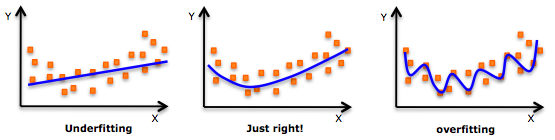
\includegraphics[width=7.71in]{images/penalized_overfitting} 

}

\caption{과적합의 예.}\label{fig:unnamed-chunk-202}
\end{figure}

\hypertarget{bias-variance-tradeoff}{%
\section{Bias-Variance tradeoff}\label{bias-variance-tradeoff}}

\hypertarget{ridge-regression}{%
\section{능형회귀(ridge regression)}\label{ridge-regression}}

앞서 말한 문제점의 한 가지 해결방법으로 추정량의 불편성을 약간 깨는 방법이 있다. \citep{Hoerl1970}은 \(X^{T}X\)에 작은 상수값 \(\lambda\)를 더해 역을 취해 추정량의 불안정성을 해결할 수 있다고 생각하고 다음과 같은 추정량을 제안하였다.
\[\hat{\beta}_{ridge}=(X^{T}X+\lambda I_{p})^{-1}X^{T}Y.\]
이를 \textbf{능형회귀(ridge regression)} 추정량이라고 부른다. 참고로 수학에서는 이 방법을 \href{https://en.wikipedia.org/wiki/Tikhonov_regularization}{Tikhonov regularization}이라고 부른다.

\(\hat{\beta}_{ridge}\)는 다음 벌점화제곱합
\[\hat{\beta}^{rodge}=\text{arg}\min_{\beta}\{\sum_{i=1}^{n}(y_{i}-\beta_{0}-\sum_{j=1}^{p}x_{ij}\beta_{j})^{2}+\lambda\sum_{j=1}^{p}\beta_{j}^{2}\}\]
을 최소화하여 얻을 수 있다. 또 다른 표현으로는
\[\hat{\beta}^{rodge}=\text{arg}\min_{\beta}\sum_{i=1}^{n}(y_{i}-\beta_{0}-\sum_{j=1}^{p}x_{ij}\beta_{j})^{2}\text{ for some } t, \sum_{j=1}^{p}\beta_{j}^{2}<t^{2}\]
로도 쓸 수 있다.

벌점화 항을 살펴보면, \(\lambda\)는 미리 선택된 상수(constant)에 벡터 \(\beta\)의 제곱합이 곱해진 형태이다. 이는 \(\beta_{j}\)가 큰 값을 가지면 페널티를 주겠다는 뜻이다. \(\beta_{j}\)가 0에 가까울수록 벌점화 항은 작을 것이다.

\hypertarget{--geometrical-interpretation-of-ridge-regression}{%
\subsection{능형회귀의 기하학적 해석(geometrical interpretation of ridge regression)}\label{--geometrical-interpretation-of-ridge-regression}}

\begin{figure}

{\centering 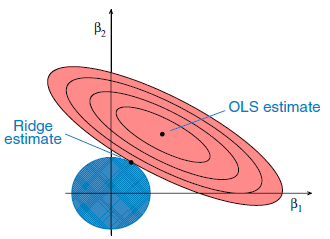
\includegraphics[width=4.58in]{images/basic_ridge} 

}

\caption{Geometric interpretation of ridge regression.}\label{fig:unnamed-chunk-203}
\end{figure}

\(p=2\)인 경우를 생각해보자. 등고선이 있는 붉은색 타원이 residual sum of squares (RSS)에 해당하며 가장 안쪽에 있는 원이 작은 RSS를 가지고 그 중심에 \(\hat{\beta}_{OLS}\)가 있다. \(p=2\)일 때 능형회귀의 제약조건은 원에 대응된다. 능형회귀의 해는 타원과 원이 만나는 지점이 될 것이다.

여기서 penalty term과 RSS 사이에는 trade-off가 있다고 한다.

\hypertarget{-properties-of-ridge-estimator}{%
\subsection{능형회귀추정량의 성질들(properties of ridge estimator)}\label{-properties-of-ridge-estimator}}

\hypertarget{svd----computing-the-ridge-solutions-via-the-svd}{%
\subsection{SVD를 이용한 능형회귀 해의 계산(computing the ridge solutions via the SVD)}\label{svd----computing-the-ridge-solutions-via-the-svd}}

능형회귀의 해

\[\hat{\beta}_{ridge}=(X^{T}X+\lambda I_{p})^{-1}X^{T}Y\]

를 다시 상기해보자. \(\hat{\beta}_{ridge}\)를 구할 때 피하고 싶은 역행렬의 계산이 있다. 수치적으로 불안정할 뿐더러 계산량이 대략 \(\mathcal{O}(p^{3})\) 정도 된다. 역행렬의 계산을 피할 수 있는 방법으로 SVD를 이용하는 방법이 있다. 즉

\[X=UDV^{T}\]

임을 이용해 해를 계산하는 것이다.

\hypertarget{lasso}{%
\section{라쏘(LASSO)}\label{lasso}}

능형회귀는 축소 추정치를 주지만 변수선택은 하지 않는다. 따라서 고차원 자료의 경우 최종 모형에 대한 해석이 그리 용이하지 않다.

\hypertarget{lmm}{%
\chapter{선형혼합모형}\label{lmm}}

\hypertarget{linear-mixed-model}{%
\section{선형혼합모형(linear mixed model)}\label{linear-mixed-model}}

이 부분의 내용은\citep{Wood2006}를 참고하였다. 일반적으로 \textbf{선형혼합모형(linear mixed model)}은 선형모형을 확장한 것이다.
\[\mathbf{y}=\mathbf{X}\boldsymbol{\beta}+\boldsymbol{\epsilon}, \qquad{\boldsymbol{\epsilon}\sim\mathcal{N}(0,\boldsymbol{\Lambda}_{\theta})}.\]
이 때
\[\mathbf{y}=\mathbf{X}\boldsymbol{\beta}+\mathbf{Zb}+\boldsymbol{\epsilon},\]
\[\mathbf{b}\sim\mathcal{N}(\mathbf{0},\boldsymbol{\psi}_{\theta}),\]
\[\boldsymbol{\epsilon}\sim\mathcal{N}(\mathbf{0},\boldsymbol{\Lambda}_{\theta})\]
이다. \(\mathbf{b}\)는 무작위 벡터로 \textbf{무작위 효과(random effects)}를 나타낸다. \(\mathbf{b}\)는 기댓값이 0이고 공분산 행렬은 알려지지 않은 모수 \(\theta\)를 포함한 \(\boldsymbol{\psi}_{\theta}\)를 갖는다. \(\mathbf{Z}\)는 무작위 효과를 나타내는 모형 행렬(model matrix)이다. \(\boldsymbol{\Lambda}_{\theta}\)는 양정치(positive definite) 행렬로 residual의 autocorrelation을 모델링하는데 사용한다. 만약 \(\boldsymbol{\Lambda}_{\theta}=\mathbf{I}\sigma^{2}\)이면 \(\mathbf{b}\)와 \(\boldsymbol{\epsilon}\)은 독립이다.

\hypertarget{----a-single-random-factor}{%
\subsection{무작위 요인인 한 개일 때(a single random factor)}\label{----a-single-random-factor}}

\citep{Wood2006}를 참고하였다. 이 때의 모형은
\[y_{ij}=\alpha +b_{i}+\epsilon_{ij}\]
이다. 이때 \(\alpha\)는 모집단의 평균에 대한 고정된 모수 \(i=1,\ldots, I, j=1,\ldots, J\)이고 \(b_{i}\sim\mathcal{N}(0,\sigma_{b}^{2})\), \(\epsilon_{ij}\sim\mathcal{N}(0,\sigma^{2})\)이다. 그리고 모든 \(b_{i}\)와 \(\epsilon_{e_{ij}}\)는 서로 독립이다.

\hypertarget{----a-model-with-two-factors}{%
\subsection{무작위 요인인 두 개일 때(a model with two factors)}\label{----a-model-with-two-factors}}

\(i\)레벨 고정 효과 \(A\)와 \(j\)레벨 무작위 효과 \(B\)에 대한 \(k\)번째 관찰값에 대한 모형은 다음과 같다.
\[y_{ijk} = \mu + \alpha_{i} + b_{j} + (\alpha b)_{ij} + \epsilon_{ijk},\]
여기서 \(b_{j}\sim \mathcal{N}(0,\sigma_{b}^{2})\), \((\alpha b)_{ij}\sim \mathcal{N}(0,\sigma_{\alpha b}^{2})\) 그리고 \(\epsilon_{ijk}\sim \mathcal{N}(0,\sigma^{2})\)이며 이 확률변수들은 mutually independent이다. \(\mu\)는 overall population mean이며 \(\alpha_{i}\)는 요인 \(A\)에 대한 \(I\)가지 고정 효과들이고 \(b_{j}\)는 요인 \(B\)에 대한 \(J\)가지 무작위 요인들이며 \((\alpha b)_{ij}\)는 요인들간의 \(IJ\) 상호효과를 나타내는 항이다.

\hypertarget{---maximum-likelihood-estimaton-for-mixed-model}{%
\section{혼합모형에 대한 최대가능도 추정(maximum likelihood estimaton for mixed model)}\label{---maximum-likelihood-estimaton-for-mixed-model}}

최소자승법보다 혼합모형에 대한 좀 더 일반적인 접근 방법은 일반화선형모형처럼 최대가능도 추정(maximum likelihood estimaton, MLE)을 하는 것이다. 자료 벡터 \(\mathbf{y}\)에 대한 통계적 모형은 확률밀도함수 \(f_{\theta}(\mathbf{y})\)를 정의한다. \(\boldsymbol{\theta}\)는 모형의 알려지지 않은 모수에 해당한다. MLE의 가장 키가 되는 아이디어는 \(f_{\theta}(\mathbf{y})\)가 큰 쪽에 진짜 \(\boldsymbol{\theta}\)가 있을 가능성이 높다는 것이다.

\hypertarget{---numerical-likelihood-maximization}{%
\subsection{가능도 최대화의 수치적 방법(numerical likelihood maximization)}\label{---numerical-likelihood-maximization}}

로그-가능도를 직접 최대화할 수 있는 경우는 흔치 않으며, 주로 수치적 최적화 방법이 필요하다. 속도와 신뢰성 향상을 위해 뉴턴 방법의 변형된 방법들이 주로 선택되어진다. 또한 이 방법은 로그-가능도의 헤시안을 구해야 한다. 그리고 \(l(\boldsymbol{\theta})\)를 최대화하는 것은 \(-l(\boldsymbol{\theta})\)를 최소화하는 것과 같다.

뉴턴 방법의 기본 원리는 \(l(\boldsymbol{\theta})\)를 지금 상태의 모수 추측 \(\boldsymbol{\theta}_{0}\)을 이용해 2차 테일러 전개로 근사하는 것이다. 그리고 \(l(\boldsymbol{\theta}')<l(\boldsymbol{\theta}_{0})\)일 경우 새로 얻어진 \(l(\boldsymbol{\theta}')\)가 \(l(\boldsymbol{\theta}_{0})\)보다 작지 않을 때까지 \(\boldsymbol{\theta}' \leftarrow \frac{\boldsymbol{\theta}' + \boldsymbol{\theta}_{0}}{2}\)로 바꿔준다. 이런 과정들은 \(\frac{\partial l}{\partial \boldsymbol{\theta}}\approx 0\)이 될때까지 반복한다.

\hypertarget{--linear-mixed-model-in-general}{%
\section{일반적인 선형 혼합모형(linear mixed model in general)}\label{--linear-mixed-model-in-general}}

일반적인 선형 혼한 모형은 다음과 같이 쓸 수 있었음을 상기하자.
\[\mathbf{y}=\mathbf{X}\boldsymbol{\beta}+\mathbf{Zb}+\boldsymbol{\epsilon},\]
\[\mathbf{b}\sim\mathcal{N}(\mathbf{0},\boldsymbol{\psi}_{\theta}),\]
\[\boldsymbol{\epsilon}\sim\mathcal{N}(\mathbf{0},\boldsymbol{\Lambda}_{\theta}),\]
여기서 \(\boldsymbol{\psi}_{\theta})\)는 무작위 효과 \(\mathbf{b}\)에 대한 양정치 공분산 행렬이고 \(\mathbf{Z}\)는 고정된 계수들이 반응변수에 어떤 영향을 미치는지 묘사하는 행렬이다(random effect와 관련, 즉 random effects에 대한 model matrix). \(\boldsymbol{\psi}_{\theta})\)는 어던 모수들 \(\boldsymbol{\theta}\)와 연관되는데 이들은 random effect에 관한 추론을 할 때 최우선 타겟이 된다. \(\boldsymbol{\Lambda}_{\theta})\)는 양정치 행렬이며 몇개의 알려지지 않은 모수들에 의존한다. 가장 단순하게는 \(\mathbf{I}\sigma^{2}\)이 될 수 있다.

또한 \(\mathbf{y}\)를 다음과 같이 다변량 정규 분포 형태로 쓸 수 있다.
\[\mathbf{y} \sim \mathcal{N}(\mathbf{X}\boldsymbol{\beta}, \mathbf{Z}\boldsymbol{\psi}_{\theta}\mathbf{Z}^{T}+\boldsymbol{\Lambda}_{\theta}).\]

\hypertarget{--maximum-likelihood-estimaton-for-linear-mixed-model}{%
\section{선형 혼합모형의 최대가능도추정(maximum likelihood estimaton for linear mixed model)}\label{--maximum-likelihood-estimaton-for-linear-mixed-model}}

\hypertarget{reml}{%
\subsection{REML}\label{reml}}

분산성분들에 관한 최대가능도 추정의 가장 큰 문제는 과소추정(underestimate)할 가능성이 높다는 것이다. 가장 명백한 예제로 선형모형의 \(\sigma^{2}\)에 대한 최대가능도추정은 \(\hat{\theta}^{2} = \frac{\|\mathbf{y}-\mathbf{X}\boldsymbol{\beta} \|^{2}}{n}\)이다. 이것은 분명히 불편추정량이 아니다.

\textbf{Restricted maximum likelihood (REML)}은 최대가능도 대신 편차를 줄이기 위해 고안되었다. 제한된 가능도는 \(f(\mathbf{y}, \mathbf{b}|\boldsymbol{\beta})\)를 \(\mathbf{b}\)와 \(\boldsymbol{\beta}\)에 대해 적분함으로써 얻을 수 있다. 결과는 다음과 같다.

\begin{align*}
2l_{r}(\boldsymbol{\theta})&=-\|\mathbf{y}-\mathbf{X}\hat{\boldsymbol{\beta}}-\mathbf{Z}\hat{\mathbf{b}} \|_{\Lambda_{\theta}^{-1}}^2-\hat{\mathbf{b}}^{T}\boldsymbol{\psi}_{\theta}^{-1}\hat{\mathbf{b}}-\log|\boldsymbol{\Lambda}_{\theta}|-\log |\boldsymbol{\psi}_{\theta}|\\
&- \log
\begin{bmatrix}
\mathbf{Z}^{T}\boldsymbol{\Lambda}_{\theta}^{-1}\mathbf{Z}+\boldsymbol{\psi}_{\theta}^{-1} & \mathbf{Z}^{T}\boldsymbol{\Lambda}_{\theta}^{-1}\mathbf{X}\\
\mathbf{X}^{T}\boldsymbol{\Lambda}_{\theta}^{-1}\mathbf{Z} & \mathbf{X}^{T}\boldsymbol{\Lambda}_{\theta}^{-1}\mathbf{X}
\end{bmatrix}
-(n-M)\log(2\pi).
\end{align*}

이 때 \(M\)은 \(\boldsymbol{\beta}\)의 차원이며 \(\hat{\boldsymbol{\beta}}\)와 \(\hat{\mathbf{b}}\)는 \(\boldsymbol{\theta}\)에 의존적이므로 각각의 \(\boldsymbol{\theta}\)에 대해서 다 계산해줘야 한다. Restrict log likelihood \(l_{r}\)은 AIC 등의 test statistic을 사용할 수 있다. 그러나 different fixed effect structure를 가진 모형끼리는 비교할 수 없다.

\hypertarget{r--linear-mixed-models-in-r}{%
\section{R 예제 (linear mixed models in R)}\label{r--linear-mixed-models-in-r}}

\hypertarget{glm}{%
\chapter{일반화선형모형}\label{glm}}

\citep{Nelder1972}는 몇가지 중요한 회귀분석 모형들을 통합한 개념인 \textbf{일반화선형모형(generalized linear model, GLM)}을 발표하였다. 이 논문에서 \textbf{포아송 회귀(Poisson regression)}와 \textbf{로지스틱 회귀(logistic regression)}가 GLM의 특수한 경우임을 보이고 추정을 위해 \textbf{반복재가중최소제곱(iteratively reweighted least squares, IRLS)} 알고리즘이 사용될 수 있음을 보였다.

\hypertarget{-glm-basics}{%
\section{일반화선형모형의 기본(GLM basics)}\label{-glm-basics}}

다음과 같은 독립인 샘플 자료 \((\mathbf{x}_{i}, y_{i}), i=1,\ldots, n\)이 있다고 하자. 이 떄 \(y_{i}\)는 반응변수, \(n\)은 표본의 크기 그리고 \(\mathbf{x}_{i}=(x_{i1},\ldots, x_{ip})^{T}\)는 \(p\)개의 설명변수들의 벡터이다. (\(x_{i1}=1\)로 보통 놓는다)

\textbf{일반화선형모형(generalized linear model)}은 일반적으로 다음의 세 개의 파트로 구성된다.

\begin{enumerate}
\def\labelenumi{\arabic{enumi}.}
\item
  \textbf{random component}: \(f(y;\mu)\)는 \(Y\)의 분포를 특정한다.
\item
  \textbf{systematic component}: \(\eta = \boldsymbol{\beta}^{T}\mathbf{x}\)는 알려진 설명변수들로 설명될 수 있는 \(Y\)의 variation을 특정한다.
\item
  \textbf{link function}: \(g(\mu)=\boldsymbol{\beta}^{T}\mathbf{x}\)는 이 둘을 묶는 역할을 한다. 종종 \(g\)는 단순히 \textbf{링크(link)}라고 불리기도 한다.
\end{enumerate}

\(\eta\)는 \textbf{선형예측변수(linear predictor)}로 알려져있다. 무작위 성분 \(f(y;\mu)\)는 보통 \(E(Y|\mathbf{x})=\mu(\mathbf{x})\)인 지수족분포(평균함수)로 모델링한다. GLM은 \(g\)가 알려져 있을 때 다음과 같은 모형을 적합한다.
\[g(\mu(\mathbf{x}_{i}))=\eta_{i}=\boldsymbol{\beta}^{T}\mathbf{x}_{i}=\beta_{1}x_{i1}+\ldots+\beta_{p}x_{ip}.\]
이 때 \(g\)는 strictly monotonicity해야 하고 \(\mu\)의 range에서 적어도 두 번 미분이 가능해야 한다. \(g\)의 주된 역할은 평균을 변환시켜 최적화 문제가 잘 작동하도록 하는 것이다. 벡테 GLM 표현으로는 위 식을 다음과 같이 표현한다.
\[g_{1}(\mu(\mathbf{x}_{i}))=\eta_{i1}=\boldsymbol{\beta}_{1}^{T}\mathbf{x}_{i}=\beta_{(1)1}x_{i1}+\ldots+\beta_{(1)p}x_{ip}.\]
즉 모형에 한 개 이상의 선형번수를 허락하는 것이다.

관찰값이 한 개 있을때, 지수족의 확률밀도함수는 다음과 같이 쓸 수 있다.
\[f(y;\theta, \phi)=\exp\{ \frac{y\theta-b(\theta)}{a(\phi)} +c(y,\phi) \}.\]
이 때 \(\theta\)는 \textbf{자연모수(natural parameter)} 또는 \textbf{정준모수(canonical parameter)}로 불리고, \(\phi\)는 \textbf{산포모수(dispersion parameter)}라고 불린다. 그리고 \(a,b,c\)는 알려진 함수들이다. \(\phi\)가 알려졌으면, \(Y\)의 분포는 one-parameter canonical exponential family member가 된다. \(\phi\)가 알려져있지 않을 때에는 이것은 nuisance parameter가 되며 주로 method of moments로 추정된다. 많은 GLM 이론에서 \(\phi\)는 알려져 있지 않다고 하다라도 모수로 취급하지 않고 상수로 취급하는 경향이 있다.

\BeginKnitrBlock{example}[정규분포는 지수족의 멤버]
\protect\hypertarget{exm:unnamed-chunk-204}{}{\label{exm:unnamed-chunk-204} \iffalse (정규분포는 지수족의 멤버) \fi{} }정규분포는 다음과 같이 지수족으로 표현할 수 있다.
\begin{align*}
f(y;\mu)&=\frac{1}{\sigma\sqrt{2\pi}}\exp[-\frac{(y-\mu)^{2}}{2\sigma^{2}}]\\
&=\exp[\frac{-y^{2}+2y\mu -\mu^{2}}{2\sigma^{2}}-\log (\sigma\sqrt{2\pi})]\\
&=\exp[\frac{y\mu -\mu^{2}/2}{\sigma^{2}}-\frac{y^{2}}{2\sigma^{2}}-\log (\sigma\sqrt{2\pi})]
\end{align*}
이 때 \(\theta=\mu\), \(b(\theta)=\theta^{2}/2\equiv \mu^{2}/2\), \(a(\phi)=\phi=\sigma^{2}\)이고 \(c(\phi,y)=-y^{2}/(2\phi) -\log(\sqrt{\phi 2\pi})\equiv -y^{2}/(2\sigma^{2})-\log(\sigma\sqrt{2\pi})\)가 된다.
\EndKnitrBlock{example}

지수족 분포의 평균과 분산에 대해 \(a,b,\phi\)를 이용하여 좀 더 일반적인 표현을 얻는 것도 가능하다. \(y\)가 주어졌을 때 \(\theta\)의 로그 가능도를 추정하는 것은 단순히 \(\log\{f(y;\theta)\}\)를 \(\theta\)에 대한 함수로 생각하면 된다. 즉
\[l(\theta)= \frac{y\theta-b(\theta)}{a(\phi)} +c(y,\phi)\]
이며 따라서 이것의 편미분은 \(l\)을 확률변수로 다룸으로써 얻을 수 있다.
\[\frac{\partial l}{\partial \theta}=\frac{y-b'(\theta)}{a(\phi)}.\]
특별한 관찰값 \(y\)를 확률변수로 대체하면 \(\frac{\partial l}{\partial \theta}\)의 기댓값을 구하는 것이 가능하다.
\[\mathbb{E}(\frac{\partial l}{\partial \theta})=\frac{\mathbb{E}(Y)-b'(\theta)}{a(\phi)}.\]
\(\mathbb{E}(\frac{\partial l}{\partial \theta})=0\)으로 하고 다시 정렬하면 다음과 같은 식을 얻을 수 있다.
\[\mathbb{E}(Y)=b'(\theta).\]
이 말은 즉슨, 어떤 지수족 확률변수의 기댓값은 \(b\)를 \(\theta\)에 대해 한 번 미분함으로써 얻을 수 있다는 것이다. 가능도를 한 번 더 미분하면 다음 식을 얻는다.
\[\frac{\partial^{2} l}{\partial \theta^{2}}=-\frac{b''(\theta)}{a(\phi)}.\]
이것을 일반적인 결과에 넣으면, \(\mathbb{E}(\frac{\partial^{2} l}{\partial \theta^{2}})=-\mathbb{E}\{(\frac{\partial l}{\partial \theta})^{2}\}\)를 얻는다. 또한 이것을 이용해 다음 식을 얻을 수 있다.
\[\frac{b''(\theta)}{a(\phi)}=\frac{\mathbb{E}[\{Y-b'(\theta)\}^{2}]}{a(\phi)^{2}}.\]
잘 정리하면 다음과 같은 일반적인 결과를 얻을 수 있다.
\[\text{var}(Y)=b''(\theta)a(\phi).\]
만약 우리가 \(\theta\)를 알고 있다면 GLM을 다루는 데 어떤 어려움도 없다. 그러나 만약 우리가 \(\phi\)를 모르고 있다면 \(a(\phi)=\frac{\phi}{A}\) (\(A\)는 알려진 상수)로 표현할 수 있지 않는 이상 상황이 어려워진다.

\hypertarget{-fitting-generalized-linear-models}{%
\subsection{일반화선형모형의 적합(fitting generalized linear models)}\label{-fitting-generalized-linear-models}}

이 부분은 \citep{Wood2006}을 참고하였다. 독립 설명변수들의 \(n\)-벡터 \(\mathbf{Y}\)의 GLM 모형이
\[g(\mu_{i})=\mathbf{X}_{i}\boldsymbol{\beta}, \qquad{Y_{i}\sim f(y_{i};\theta_{i})}\]
라고하자. 이 때 \(f(y_{i};\theta_{i})\)는 지수족 분포를 나타내며 \(\theta\)는 \(\mu_{i}\)에 의해(즉 궁극적으로 \(\boldsymbol{\beta}\)에 의해)결정되는 정준모수다. \(\mathbf{Y}\)의 관찰값 \(\mathbf{y}\)가 주어졌을 때, \(\boldsymbol{\beta}\)의 최대우도추정이 가능하다. \(Y_{i}\)는 상호 독립이라고 했으므로, \(\boldsymbol{\beta}\)의 가능도는 다음과 같다.
\[L(\boldsymbol{\beta})=\prod_{i=1}^{n}f(y_{i};\theta_{i}).\]
따라서 \(\boldsymbol{\beta}\)의 로그-가능도는
\[l(\boldsymbol{\beta})=\sum_{i=1}^{n}\log \{ f(y_{i};\theta_{i}) \}=\sum_{i=1}^{n}\frac{y_{i}\theta_{i}-b_{i}(\theta_{i})}{a_{i}(\phi)}+c_{i}(\phi,y_{i})\]
이다. 어떤 경우에는 \(a,b,c\)가 \(i\)에 따라 달라질 수도 있다. 한편 \(\phi\)는 \(i\)에 따라 보통 같다고 놓는다. 앞 절에서 논의한대로 가장 간단한 \(a_{i}(\phi)=\frac{\phi}{A_{i}}\) (이 때 \(A_{i}\)는 알려진 상수, 주로 1)를 가정하자. 그러면
\[l(\boldsymbol{\beta})=\sum_{i=1}^{n}A_{i}\frac{y_{i}\theta_{i}-b_{i}(\theta_{i})}{\phi}+c_{i}(\phi,y_{i})\]
가 된다. 이 로그-가능도를 최대화하기 위해서는 보통 \textbf{뉴턴의 방법(Newton's method)}를 사용한다. 이것은 \(l\)의 그라디언트 벡터와 헤시안을 계산해야 한다.
\[\frac{\partial l}{\partial \beta_{j}}=\frac{1}{\phi}\sum_{i=1}^{n}A_{i}\Big( y_{i}\frac{\partial \theta_{i}}{\partial \beta_{j}}-b_{i}'(\theta_{i})\frac{\partial \theta_{i}}{\partial \beta_{j}}   \Big).\]
또한 \textbf{체인룰(chain rule)}에 따라
\[\frac{\partial \theta_{i}}{\partial \beta_{j}}=\frac{d\theta_{i}}{d\mu_{i}}\frac{\partial\mu_{i}}{\partial \beta_{j}} =\frac{d\theta_{i}}{d\mu_{i}}\frac{\partial\eta_{i}}{\partial \beta_{j}}\frac{d\mu_{i}}{d\eta_{i}}=\frac{X_{ij}}{g'(\mu_{i})b''(\theta_{i})}.\]
마지막 등식은 \(\frac{d\mu_{i}}{d\eta_{i}}=g'(\mu_{i})\) 그리고 \(\frac{\partial\eta_{i}}{\partial \beta_{j}}=X_{ij}\), \(\frac{d\theta_{i}}{d\mu_{i}}=\frac{1}{b;;(\theta_{i})}\)라는 사실로부터 얻어진다. 이들을 잘 정리하면,
\[\frac{\partial l}{\partial \beta_{j}}=\frac{1}{\phi}\sum_{i=1}^{n}\frac{y_{i}-b_{i}'(\theta)}{g'(\mu_{i})b_{i}''(\theta_{i})/A_{i}}X_{ij}=\frac{1}{\phi}\sum_{i=1}^{n}\frac{y_{i}-\mu_{i}}{g'(\mu_{i})V(\mu_{i})}X_{ij}\]
를 얻는다. 다시 미분하면 다음을 얻는다.

\begin{align*}
\frac{\partial^{2}l}{\partial \beta_{j}\partial \beta_{k}}&=-\frac{1}{\phi}\sum_{i=1}^{n}\Big\{ \frac{X_{ik}X_{ij}}{g'(\mu_{i})^{2}V(\mu_{i})} - \frac{(y_{i}-\mu_{i})V'(\mu_{i})X_{ik}X_{ij}}{g'(\mu_{i})^{2}V(\mu_{i})^{2}}+\frac{(y_{i}-\mu_{i})X_{ij}g''(\mu_{i})X_{ik}}{g'(\mu_{i})^{3}V(\mu_{i})} \Big\}\\
&-\frac{1}{\phi}\sum_{i=1}^{n}\frac{X_{ik}X_{ij}\alpha(\mu_{i})}{g'(\mu_{i})^{2}V(\mu_{i})}.
\end{align*}

이 때 \(\alpha(\mu_{i})= 1+ (y_{i}-\mu_{i})\{ \frac{V'(\mu_{i})}{V(\mu_{i})} + \frac{g''(\mu_{i})}{g'(\mu_{i})} \}\)이다. 표현 \(\mathbb{E}(\frac{\partial^{2}l}{\partial \beta_{j}\partial \beta_{k}})\) 또한 똑같지만, \(\alpha(\mu_{i})= 1\)이다. 따라서 \(\mathbf{W}=\text{diag}(w_{i})\), \(w_{i}=\frac{a(\mu_{i})}{g'(\mu_{i})^{2}V(\mu_{i})}\)로 정의하면, 로그-가능도의 헤시안은 \(-\frac{\mathbf{XWX}}{\phi}\)가 되며, 헤시안의 기댓값은 \(\alpha(\mu_{i})=1\)로 놓음으로써 얻을 수 있다. \(\alpha(\mu_{i})=1\)로 계산된 가중치들을 \textbf{피셔 가중치(Fisher weight)}들이라고 부른다. \(\mathbf{G}=\text{diag}\{\frac{g'(\mu_{i})}{\alpha(\mu_{i})}\}\)로 정의함으로써, 그라디언트 벡터의 로그-가능도는 \(\frac{\mathbf{X}^{T}\mathbf{WG}(\mathbf{y}-\boldsymbol{\mu})}{\phi}\)가 된다. 그러면 뉴턴 업데이트는 다음과 같은 형태를 갖는다.

\begin{align*}
\boldsymbol{\beta}^{[k+1]}&=\\boldsymbol{\beta}^{[k]}+(\mathbf{XWX})^{-1}\mathbf{X}^{T}\mathbf{WG}(\mathbf{y}-\boldsymbol{\mu})\\
&=(\mathbf{XWX})^{-1}\mathbf{X}^{T}\mathbf{W}\{\mathbf{G}(\mathbf{y}-\boldsymbol{\mu})+\mathbf{X}\boldsymbol{\beta}^{[k]}\}\\
&-(\mathbf{XWX})^{-1}\mathbf{X}^{T}\mathbf{W}\mathbf{z}.
\end{align*}

이 때 \(z_{i}=g'(\mu_{i})\frac{y_{i}-\mu_{i}}{\alpha(\mu_{i})}+\eta_{i}\)이다. (\(\boldsymbol{\eta}\equiv\mathbf{X}\boldsymbol{\beta}\)이다.) 결국 이 이생 방정식은 \(\boldsymbol{\beta}\)에 대한 가중 최소자승방법 중 하나라고 볼 수 있다.

결국 GLM은 \textbf{반복 재가중 최소자승(iteratively re-weighted least squares)} 알고리즘으로 추정되 수 있으며, 다음과 같다.

\begin{enumerate}
\def\labelenumi{\arabic{enumi}.}
\item
  \(\hat{\mu}_{i}=y_{i}+\delta_{i}\), \(\hat{\eta}_{i}=g(\hat{\mu}_{i})\)로 초기화한다. \(\delta_{i}\)는 보통 0으로 놓으며, \(\hat{\eta}_{i}\)가 유한함을 보장하기 위해 작은 상수일 수도 있다. 수렴할 때까지 아래 두 단계를 반복한다.
\item
  Pseudo-data \(z_{i}=g'(\hat{\mu}_{i})\frac{y_{i}-\hat{\mu}_{i}}{\alpha(\hat{\mu}_{i})}+\hat{\eta}_{i}\)와 반복 가중치 \(w_{i}=\frac{a(\hat{\mu}_{i})}{g'(\hat{\mu}_{i})^{2}V(\hat{\mu}_{i})}\)를 계산한다.
\item
  가중 최소자승
  \[\sum_{i=1}^{n}w_{i}(z_{i}-\mathbf{X}_{i}\boldsymbol{\beta})^{2}\]
  을 최소화하는 \(\hat{\boldsymbol{\beta}}\)를 찾는다. 그리고 \(\hat{\boldsymbol{\eta}}=\mathbf{X}\hat{\boldsymbol{\beta}}\)로, \(\hat{\mu}_{i}=g^{-1}(\hat{\eta}_{i})\)로 갱신한다.
\end{enumerate}

\hypertarget{-univariate-smoothing}{%
\section{일변량 스므딩(univariate smoothing)}\label{-univariate-smoothing}}

\citep{Yee2015}에 따르면 스므더(smoother)의 종류에는 다음이 있다.

\begin{enumerate}
\def\labelenumi{\arabic{enumi}.}
\item
  Regression or series smoothers (polynomial regression, regression splines, P-splines, Fourier regression, filtering, wavelets)
\item
  Smoothing splines (with roughness penalties, e.g., cubic smoothing splines, O-splines, P-splines)
\item
  Local regression (Nadaraya-Watson estimator, kernel smoothers, Lowess, Loess, it generalizes to local likelihood)
\item
  Nearest-neighbour smoothers (running means, running lines, running medians)
\end{enumerate}

\textbf{고전적인 스므딩 문제(classical smoothing problem)}는 다음 모형에 대해 임의의 부드러운 함수(smooth function) \(f\)를 추정하는 문제이다.

\[y_{i}=f(x_{i})+\epsilon_{i}, \qquad{\epsilon_{i} \sim  (0, \sigma_{i}^{2})}\]

일반적으로 자료를 \(x_{1}<x_{2}<\ldots <x_{n}\) 등으로 크기에 따라 정렬할 수 있다고 가정하면, 모든 스므딩 방법의 기본 아이디어는 \textbf{이웃(neighbourhood)}을 정의하는 것이다. 타겟 포인트 \(x_{0}\)가 있을때 이것의 이웃의 크기를 정하는 일은 함수의 부드러움을 결정하는 문제와 같이 때문에 매우 중요하다.

\hypertarget{-vector-generalized-linear-models}{%
\section{벡터 일반화선형모형(vector generalized linear models)}\label{-vector-generalized-linear-models}}

이 절의 내용은 \citep{Yee2015}를 따른다.

\hypertarget{-limations-of-glm}{%
\section{일반화선형모형의 한계점(limations of glm)}\label{-limations-of-glm}}

\citep{Yee2015}에 의하면 GLM은 잘 알려진 지수족 내의 일차원 분포에서만 잘 적용된다는 한계점을 가지고 있다.

\hypertarget{gam}{%
\chapter{일반화가법모형}\label{gam}}

일반화가법모형을 처음 다룬 논문들로는 \citep{Hastie1986}이 있다. 일반화가법모형에 대한 참고문헌으로는 \citep{Wood2006}이 있다. 최근에 나온 좋은 책으로는 \citep{Yee2015}가 있으며 이 책은 주로 \textbf{벡터 일반화선형모형(vector genearlized linear model, VGLMs)} 및 \textbf{벡터 일반화가법모형(vector generalized addtive model, VGAMs)}에 초점을 맞추고 있고 R 코드를 포함하고 있다.

일반화가법모형은 일반화 선형모형이며 선형 predictor가 smooth functions of covariate의 합(sum) 형태로 표현된 모형을 말한다. 일반적으로는
\[g(\mu_{i})=\mathbf{A}_{i}\boldsymbol{\theta}+f_{1}(x_{1i})+f_{2}(x_{2i})+f_{3}(x_{3i})+\ldots\]
로 모형 structure를 표현할 수 있다. 이 때 \(\mu_{i}\equiv E(Y_{i})\)이고 \(Y_{i}\sim \text{EF}(\mu_{i},\phi)\)이다. \(Y_{i}\)는 설명변수들이고, \(\text{EF}(\mu_{i},\phi)\)는 평균 \(\mu_{i}\)와 척도모수(scale parameter) \(\phi\)인 지수족 분포(exponential family distribution)를 나타낸다. \(\mathbf{A}_{i}\)는 어떤 strictly parametric model components의 모형 행렬의 행(row)를 나타낸다. \(\theta\)는 대응되는 모수 벡터이다. \(f_{j}\)는 covariates들 \(x_{k}\)들의 smooth functions이다.

\hypertarget{additive-models}{%
\section{가법모형들(additive models)}\label{additive-models}}

회귀분석의 \textbf{가법모형(additive model)}은
\[E[Y|\mathbf{X}=\mathbf{x}]=\alpha+\sum_{j=1}^{p}f_{j}(x_j)\]
로 표현한다. 선형모형은 \(f_{j}(x_{j})=\beta_{j}x_{j}\)인 가법모형의 특별한 경우이다. \(f_{j}\)는 임의의 비선형 함수도 될 수 있다는 점에서 가법모형이 좀 더 일반적인 형태의 모형이라고 할 수 있다.

\hypertarget{-vector-gams}{%
\section{벡터 일반화가법모형(vector GAMs)}\label{-vector-gams}}

스므딩에는 다음과 같은 네 가지 종류가 있다.

\begin{enumerate}
\def\labelenumi{\arabic{enumi}.}
\item
  \(y\)는 스칼라, \(x\)는 일변량
\item
  \(y\)는 스칼라, \(\mathbf{x}\)는 다변량
\item
  \(\mathbf{y}\)는 벡터, \(x\)는 일변량
\item
  \(\mathbf{y}\)는 벡터, \(\mathbf{x}\)는 다변량
\end{enumerate}

일반적으로 얘기하는 벡터 일반화가법모형은 (3)에 해당한다.

\hypertarget{-backfitting}{%
\section{퇴각 적합화(backfitting)}\label{-backfitting}}

\textbf{퇴각 적합화(backfitting)}는 \textbf{가우스-자이델 방법(Gauss-Seidel method)}이라고도 불리는 방법으로, GAM을 적합하기 위한 단순하면서도 아름다운 방법이다. 이 알고리즘의 기본 아이디어는 가법모형의 각 smooth component들에 대해 iteratively하게 가법모형의 smooth partial residuals를 계산하는 것이다.

다음과 같은 가법모형에서 추정을 하고 싶다고 가정하자.
\[y_{i}=\alpha + \sum_{j=1}^{m}f_{j}(x_{ji})+\epsilon_{i},\]
여기서 \(f_{i}\)는 부드러운 함수들(smooth functions)이며 공변량 \(x_{j}\)는 때때로 벡터이기도 하다. \(\hat{\mathbf{f}}_{j}\)를 \(i\)째 원소의 추정값이 \(f_{j}(x_{ji})\)인 벡터라고 하자. 그러면 기본적인 퇴각 적합화 알고리즘은 다음과 같다.

\begin{enumerate}
\def\labelenumi{\arabic{enumi}.}
\item
  Set \(\alpha=\bar{y}\) and \(\hat{\mathbf{f}}_{j}=\mathbf{0}\) for \(j=1,\ldots , m\).
\item
  Repeat step 3 to 5 until teh estimates \(\hat{\mathbf{f}}_{j}=\mathbf{0}\) stop changing.
\item
  For \(j=1,\ldots ,m\), repeat steps 4 and 5.
\item
  Calculate partial residuals:
  \[\mathbf{e}_{P}^{j}=\mathbf{y}-\hat{\alpha}-\sum_{k\neq j}\hat{\mathbf{f}}_{k}.\]
\item
  Set \(\hat{\mathbf{f}}_{j}\) equal to the result of smoothing \(e_{p}^{j}\) with respect to \(x_{j}\).
\end{enumerate}

\hypertarget{---gamlss}{%
\section{위치 척도 형태모수의 일반화가법모형(GAMLSS)}\label{---gamlss}}

\hypertarget{r-r-gam}{%
\section{R 예제(R-gam)}\label{r-r-gam}}

알고리즘을 짜면 다음과 같다.

\begin{Shaded}
\begin{Highlighting}[]
\NormalTok{f<-x}\OperatorTok{*}\DecValTok{0}\NormalTok{;alpha<-}\KeywordTok{mean}\NormalTok{(y);ok <-}\StringTok{ }\OtherTok{TRUE}
\ControlFlowTok{while}\NormalTok{ (ok) \{ }\CommentTok{# backfitting loop}
  \ControlFlowTok{for}\NormalTok{ (i }\ControlFlowTok{in} \DecValTok{1}\OperatorTok{:}\NormalTok{m) \{ }\CommentTok{# loop through the smooth terms}
\NormalTok{    ep <-}\StringTok{ }\NormalTok{y }\OperatorTok{-}\StringTok{ }\KeywordTok{rowSums}\NormalTok{(f[,}\OperatorTok{-}\NormalTok{i]) }\OperatorTok{-}\StringTok{ }\NormalTok{alpha}
\NormalTok{    b <-}\StringTok{ }\KeywordTok{smooth.spline}\NormalTok{(x[,i],ep,}\DataTypeTok{df=}\NormalTok{edf[i])}
\NormalTok{    f[,i] <-}\StringTok{ }\KeywordTok{predict}\NormalTok{(b,x[,i])}\OperatorTok{$}\NormalTok{y}
\NormalTok{  \}}
\NormalTok{  rss <-}\StringTok{ }\KeywordTok{sum}\NormalTok{((y}\OperatorTok{-}\KeywordTok{rowSums}\NormalTok{(f))ˆ2)}
  \ControlFlowTok{if}\NormalTok{ (}\KeywordTok{abs}\NormalTok{(rss}\OperatorTok{-}\NormalTok{rss0)}\OperatorTok{<}\FloatTok{1e-6}\OperatorTok{*}\NormalTok{rss) ok <-}\StringTok{ }\OtherTok{FALSE}
\NormalTok{  rss0 <-}\StringTok{ }\NormalTok{rss}
\NormalTok{\}}
\end{Highlighting}
\end{Shaded}

\hypertarget{smoothing}{%
\chapter{스므딩}\label{smoothing}}

\hypertarget{-univariate-smoothing-1}{%
\section{일변량 스므딩(univariate smoothing)}\label{-univariate-smoothing-1}}

함수 모형의 표현은 보통 다음과 같은 기본적인 모형에서 출발한다.
\begin{equation}
y_{i}=f(x_{i})+\epsilon_{i}.
\label{eq:univariatesmoothing}
\end{equation}
여기서 \(y_{i}\)는 종속변수, \(x_{i}\)는 공변량, \(f\)는 부드러운 함수이며 \(\epsilon_{i}\)는 독립이며 \(\mathcal{N}(0,\sigma^{2})\)을 갖는 확률변수들이다.

\hypertarget{--representing-a-function-with-basis-expansions}{%
\subsection{함수를 기저로 표현하기(representing a function with basis expansions)}\label{--representing-a-function-with-basis-expansions}}

\(f\)를 추정하기 위해 \(f\)를 식 \eqref{eq:univariatesmoothing}를 선형모형처럼 해석하는 방법이 있다. 이렇게 하기 위해 사용하는 것이 \textbf{기저(basis)}다. 기저라 함은 \(f\)가 원소로 있는 함수 공간을 정의하는 데 필요한 것이다. \textbf{기저 함수(basis function)}들은 매우 잘 알려져 있다고 단정한다. 만약 \(b_{j}(x)\)가 \(j\)번째 기저함수라고 하면, \(f\)는 다음과 같이 표현할 수 있다고 가정한다.

\hypertarget{--the-classical-smoothing-problem}{%
\section{고전적인 스므딩 문제(the classical smoothing problem)}\label{--the-classical-smoothing-problem}}

스므딩은 탐색적 자료 분석을 위한 강력한 툴이며, 자료 기반한 방법이다. 가장 단순한 형태의 스므딩은 자료의 산점도이다. 만약 모든 점들을 그냥 잇는다면 너무 유연한 모형이 되어 과적합(overfitting)을 할 가능성이 높다. 스므더(smoother)들을 나눠보면 다음의 종류들이 있다.

\begin{enumerate}
\def\labelenumi{\arabic{enumi}.}
\item
  Regression or series smoothers (polynomial regression, regression splines, P-splines, Fourier regression, filtering, wavelets)
\item
  Smoothing splines (with roughness penalties, e.g., cubic smoothing splines, O-splines, P-splines)
\item
  Local regression (Nadayara-Watson estimator, kernel smoothers, LOWESS, LOESS, it generalizes to local likelihood)
\item
  Nearest-neighbor smoothers (running means, running lines, running medians)
\end{enumerate}

여기서 P-spline은 regression spline, smoothing spline과 유사점들을 공유하므로 일종의 하이브리드 방법이라고 볼 수 있다.

\textbf{고전적인 스므딩 문제(classical smoothing problem)}은 다음의 모형

\begin{equation}
y_{i}=f(x_{i})+\varepsilon_{i}, \qquad{\varepsilon_{i}\sim(0,\sigma_{i}^{2})}
\label{eq:classicalsmoothingproblem}
\end{equation}

으로 임의의 부드러운 함수 \(f\)를 추정하는 문제이다. 오차가 평균 9을 갖으므로 조건부 평균이 함수가 된다 \(E(Y|x)=f(x)\). 이 문제는 모든 \(\sigma_{i}\)가 동일하다고 가정하는 것이다. \(\text{Var}(\epsilon_{i})=\sigma_{i}^{2}=\sigma^{2}w_{i}^{-1}\)과 같은 분산구조에 식 \eqref{eq:classicalsmoothingproblem}을 일반화할 수도 있다.

일반성을 잃지 않고 우리는 자료를 \(x_{1}< x_{2}<\cdots <x_{n}\)으로 순서대로 놓을 수 있다. 가장 간단한 경우인 \(w_{i}=1, \forall i\)인 경우를 생각해보자. 모든 스므딩 방법들의 기본적인 아이디어는 \textbf{이웃(neighborhood)}라는 개념이다. 그 말인 즉슨 타겟이 되는 점 \(x_{0}\)와 가까운 이웃들 \(x_{i}\)들만 \(x_{0}\)에서 \(f\)를 예측할 때 쓴다는 것이다. \(x_{i}\)가 \(x_{0}\)와 가까우면 가까울수록 영향력이 커지고 \(\hat{f}(x_{0})\)를 구성하는 데 가중치를 더 많이 준다는 것이다.

이웃이라는 개념 대신 많은 사람들은 \textbf{윈도우(window)}라고 부르기도 하는데, 이 이웃을 결정하는 윈도우의 크기가 \(f\)의 부드러움 정도를 결정하기 때문에 매우 중요해진다. 이는 이것이 bias, variance와도 크게 관련이 있음을 의미한다.

\hypertarget{-polynomial-regression-in-smoothing}{%
\section{다항 회귀분석(polynomial regression in smoothing)}\label{-polynomial-regression-in-smoothing}}

\textbf{다항 회귀분석(polynomial regression)}은 \(x_{k}\)를 선형보다 더 유연하게 적합하기 위해 고차원의 항을 추가하는 것이다. Weierstrass approximation theorem에 의하면 닫힌 구간의 모든 연속 함수들은 polynomial로 uniformly approximated될 수 있다고 한다. 따라서 고차원의 항을 써서 \(f\)를 추정하는 것은 좋은 아이디어이나 항상 그렇지는 않다. 이유는 다음과 같다.

\begin{enumerate}
\def\labelenumi{\arabic{enumi}.}
\item
  다항식은 local하지 않고 global한 성질을 갖는다. 즉 왼쪽 부분에서 약간의 방해가 들어가면 오른쪽에서는 매우 큰 변화를 만든다.
\item
  Edge effect가 있다.
\item
  Outlier에 민감하다.
\item
  다항식의 차수는 연속이 아닌 이산적이다.
\end{enumerate}

\hypertarget{-regression-spline}{%
\section{회귀 스플라인(regression spline)}\label{-regression-spline}}

\citep{Yee2015}에 따르면 \textbf{회귀 스플라인(regression spline)}은 다음과 같은 장점들을 같고 있다.

\begin{enumerate}
\def\labelenumi{\arabic{enumi}.}
\item
  이 방법은 계산적, 통계적으로 단순하고 표준적인 모수 추론이 가능하다. 왜냐하면 이 방법은 부드러운 함수의 LM 표현 방법이기 때문이다.
\item
  두 번째 장점으로 어떤 매듭(knot)이 없어도 무방한지에 대한 검정이 가능하다는 것이 있다.
\end{enumerate}

그러나 이 방법에서 매듭의 숫자와 위치를 고르는 데에 어려움이 있고, 부드러움의 정도가 한 개의 스므딩 모수로는 연속적으로 조절될 수 없다는 단점도 있다.

회귀 스플라인은 기저 벡터(basis vector)들의 족(family)를 활용한 다변량 회귀분석의 일종이다. 가장 단순한 예로 \(\mathcal{S}=\{1,x,x^{2},\ldots, x^{r}\}\)로 놓으면 다항회귀분석이 된다. 이것은 \(r\)차원까지의 다항식을 기저로 놓은 것과 같다. \(r=3\)인 경우를 특별히 \textbf{3차 스플라인(cubic spline)}이라고 부른다. 이 때 우리는 \(\mathcal{S}\) spans this function space라고 부른다. 3차 스플라인에는 보통 두 개의 일반적인 기저들이 있다.

\begin{enumerate}
\def\labelenumi{\arabic{enumi}.}
\item
  Truncated power series: easy to understand, but not recommended (because of ill-conditioned).
\item
  B-splines
\end{enumerate}

\hypertarget{b-b-spline}{%
\subsection{B-스플라인(B-spline)}\label{b-b-spline}}

이 부분의 내용은 \citep{Yee2015}의 2.4.3.2절을 참고하였다. \textbf{B-스플라인(B-spline)}을 사용하는 이유는 주로 계산적인 문제 때문이라고 한다(minimal support). B-스플라인은 minimal support (또는 compact support)를 갖고 이는 spline basis끼리 the amount of overlap를 minimal하게 만드므로 안정적인 계산을 가능하게 한다고 한다.

\begin{figure}

{\centering 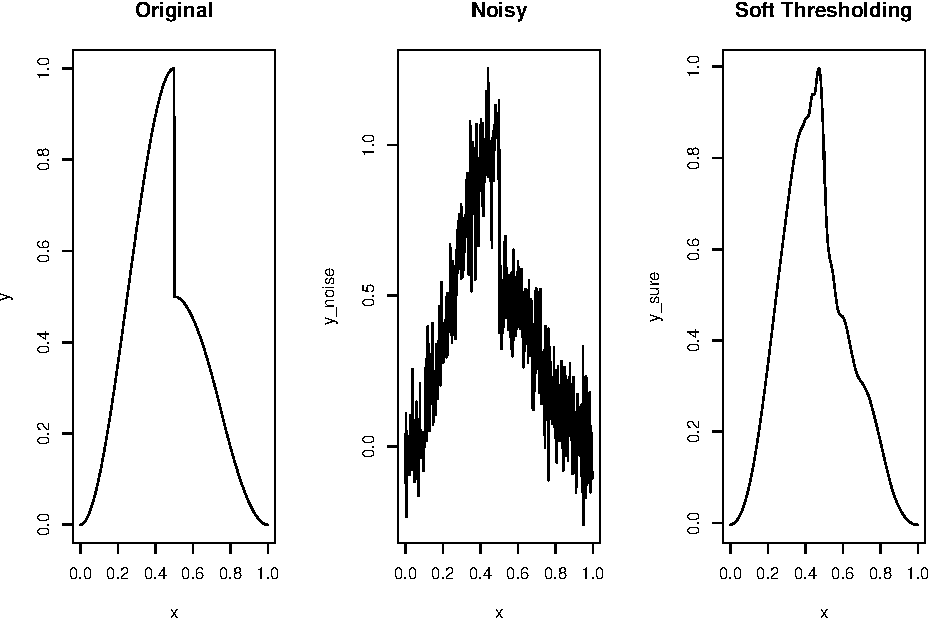
\includegraphics{book_files/figure-latex/unnamed-chunk-208-1} 

}

\caption{매듭의 위치가 0.3, 0.5, 0.6이고 Q=1,2,3,4일때의 B-스플라인 기저들.}\label{fig:unnamed-chunk-208}
\end{figure}

이것은 general order \(Q\)를 갖는 스플라인으로 생각하면 편하다. 몇 가지 특별한 경우들을 나열해 본다.

\begin{enumerate}
\def\labelenumi{\arabic{enumi}.}
\item
  \(Q=1\): unit rectangle 또는 boxcar 함수의 shifted된 버전이다.
\item
  \(Q=2\): \textbf{linear spline}이며 매듭에서 \(Q-2=0\)차 연속 미분값을 갖는다. 즉 조각별 선형함수다.
\item
  \(Q=3\): \textbf{quadratic spline}이며 매듭에서 \(Q-2=1\)차 연속 미분값을 갖는다.
\item
  \(Q=4\): \textbf{cubic spline}이며 \(f^{(Q-1)}(\xi_{s})\)안의 불연속점을 인지할 수 없는 가장 낮은 차수의 스플라인이다. \citep{Hastie2009} \textbf{Natural spline}은 cubic spline의 잘 알려진 예로 양 끝지점에서 2계, 3계도함수가 0인 스플라인이다. 즉 다음의 경계 조건들을 만족하며
  \[f''(\xi_{0})=f'''(\xi_{0})=f''(\xi_{K+1})=f'''(\xi_{K+1})=0\]
  이를 \textbf{자연경계조건(natural boundary condition)}들이라고 부른다.
\end{enumerate}

\(\xi_{s}, s=1,\ldots, K\)를 \(K\) interior knots라고 하고 \(\xi_{0}\), \(\xi_{K+1}\)를 boundary knots라고 하자. 그러면 이러한 knots들이 다음과 같은 부등식을 만족하는

\begin{alignat*}{2}
\tau_{1}\leq \tau_{2} \leq \cdots \leq \tau_{Q} &\leq \xi_{0} && \\
&< \xi_{1} \leq \cdots \leq &&\xi_{K}\\
& &&< \xi_{K+1} \leq \tau_{K+Q+1} \leq \cdots \leq \tau_{K+2Q}
\end{alignat*}
\(\boldsymbol{\tau}=(\tau_{1}, \ldots, \tau_{K+2Q})^{T}\) 벡터를 얻기 위해 \(2Q\)개의 다른 매듭들을 더 필요로 한다는 것을 알 수 있다.

\(B_{s,q}(x)\)를 order \(q\) (차수 \(q-1\), \(q=1,\ldots, Q\))을 갖고 knot sequence가 \(\boldsymbol{\tau}\)인 B-spline basis function이라고 하자. 그러면 \(B_{s,q}(x)\)는 다음과 같이 정의된다.

\begin{enumerate}
\def\labelenumi{\arabic{enumi}.}
\item
  \(s=1,\ldots, K+2-1\)일 때
  \[B_{s,1}(x)=
  \begin{cases}
  1 & \qquad{\tau_{s} \leq x < \tau_{s+1}}\\
  0 & \qquad{\text{o.w.}}
  \end{cases}\]
\item
  \(s=1,\ldots, K+2Q-q\), \(q>1\)일 때
\end{enumerate}

\begin{align*}
B_{s,q}(x)&=\omega_{s,q}B_{s,q-1}(x)+(1-\omega_{s+1,q}B_{s+1,q-1}(x))\\
&=\frac{x-\tau_{s}}{\tau_{s+q-1}-\tau_{s}}B_{s,q-1}(x) + \frac{\tau_{s+q}-x}{\tau_{s+q}-\tau_{s+1}}B_{s+1,q-1}(x),
\end{align*}

여기서 \(\omega_{s,q}\equiv (x-\tau_{s})/(\tau_{s+q-1}-\tau_{s})\) for \(\tau_{s+q-1}>\tau_{s}\)이고 만약 \(\tau_{s+q-1}=\tau_{s}\)이면 \(\omega_{s,q}\equiv 0\)이 된다. 이것들은 안정적이고 효육적인 재귀 알고리즘으로 구할 수 있다. 여기서 \(B_{s,q}\)는 \(q+1\)개의 매듭들 \(\tau_{s},\ldots, \tau_{s+q}\)에만 관련이 있고 구간 \([\tau_{s},\tau_{s+q})\) 바깥에서는 감쇄하며 구간 안에서는 양의 값을 갖는다. 만약 \(\tau_{s}=\tau_{s+q}\)이면 \(B_{s,q}=0\)이다.

\hypertarget{-smoothing-splines}{%
\section{스므딩 스플라인(smoothing splines)}\label{-smoothing-splines}}

회귀 스플라인에서 smoother의 유연성은 작은 숫자의 기저함수들만을 선택함으로써 부여할 수 있다. 그러나 많은 수의 기저 함수들을 부여한 채 시작하고 거기에 벌점화 항을 붙여줌으로써 유연한 적합 결과를 얻을 수 있는데 이러한 방법들 중 가장 유명한 접근 방법이 \textbf{3차 스므딩 스플라인(cubic smoothing spline)}이다. 이것은 다음의 목적함수

\[S(f)=\sum_{i=1}^{n}(y_{i}-f(x_{i}))^{2}+\lambda \int_{a}^{b}\{f''(x)\}^{2}dx\]
를 최소화하는 것을 찾는 것이다. 이 때 어떤 \(a,b\)에 대해 \(a < x_{1} <\ldots <x_{n} <b\)이며 \textbf{스므딩 모수(smoothing parameter)} \(\lambda\)는 \(\lambda \geq 0\)이다.

\begin{itemize}
\item
  \(S(f)\)의 첫 번째 항: residual sum of squares이며 lack-of-fit를 penalize한다.
\item
  \(S(f)\)의 두 번째 항: smoothness를 penalize한다.
\end{itemize}

두 개의 opposing quantities는 \(\lambda\)에 의해 조절된다.

\begin{itemize}
\item
  \(\lambda\rightarrow\infty\): \(f''(x)\rightarrow\infty\)이며 해는 least square line이 된다.
\item
  \(\lambda \rightarrow 0^{+}\): 해는 \((x_{i}, y_{i})\)를 정확히 보간(interpolate)하게 된다.
\end{itemize}

\hypertarget{p-p-spline}{%
\section{P-스플라인(P-spline)}\label{p-p-spline}}

\textbf{P-스플라인(P-spline)}은 penalized B-spline이라는 의미를 갖고 있다. P-스플라인은 회귀 스플라인을 인접한 B-스플라인 계수들에 벌점화를 시켜 확장한 것이다. 다음과 같이 단순한 산점도 자료 \(x_{i}\in [a,b]\)가 있다고 하자. 다음과 같이 회귀 스플라인을

\begin{equation}
f(x)=\sum_{s=1}^{K+Q-1}\beta_{s}B_{s,q}(x)
\label{eq:pspline}
\end{equation}

로 정의한다. 여기서 \(K+1\)개의 등간격 매듭들 \(\xi_{s}=a + s\frac{b-a}{K}\), \(s=0,1,\ldots, K\in [a,b]\)을 사용한다.우리는 \((\mathbf{X})_{ij}=B_{j,Q}(x_{i})\)로 둠으로써 식 \eqref{eq:pspline}를 \(\mathbf{f}=\mathbf{X}\boldsymbol{\beta}\)로 쓸 수 있다. 이때 \(\boldsymbol{\beta}\)는 다음 식을

\[S(\boldsymbol{\beta})=(\mathbf{y}-\mathbf{X}\boldsymbol{\beta})^{T}\mathbf{W}(\mathbf{y}-\mathbf{X}\boldsymbol{\beta}) + \lambda \boldsymbol{\beta}^{T}\mathbf{D}_{[d]}^{T}\mathbf{D}_{[d]}\boldsymbol{\beta}\]
를 최소화함으로써 추정할 수 있다. 이 때

\begin{itemize}
\item
  \(\lambda > 0\): 평활모수(smoothing parameter)
\item
  \(\mathbf{D}_{[d]}\): \(((K+Q-1-d)\times (K+Q-1))\)차원 행렬이며 \(d\)-차 미분 연산자 \(\Delta^{d}\)를 갖는다. 예를 들면 \(\Delta^{1}\beta_{s}=\beta_{s}-\beta_{s-1}\)이고 \(\Delta^{2}\beta_{s}=\Delta(\Delta \beta_{s})=\Delta\beta_{s}-\Delta\beta_{s-1}=\beta_{s}-\beta_{s-1}-(\beta_{s-1}-\beta_{s-2})=\beta_{s}-2\beta_{s-1}+\beta_{s-2}\)이다. 실제로는 \(d=2\) 또는 \(3\)을 많이 쓴다.
\end{itemize}

\(\frac{\partial S}{\partial \boldsymbol{\beta}}=\mathbf{0}\)으로 놓음으로써 얻는 해는
\[\boldsymbol{\beta}=(\mathbf{X}^{T}\mathbf{W}\mathbf{X}+\lambda \mathbf{D}_{[d]}^{T}\mathbf{D}_{[d]})^{-1}\mathbf{W}^{T}\mathbf{W}\mathbf{y}\]
이다. 그리고 \(\hat{\boldsymbol{\beta}}\)의 분산-공분산 행렬은
\[\text{Var}(\hat{\boldsymbol{\beta}})=\sigma^{2}(\mathbf{X}^{T}\mathbf{W}\mathbf{X}+\lambda \mathbf{D}_{[d]}^{T}\mathbf{D}_{[d]})^{-1}\mathbf{X}^{T}\mathbf{W}\mathbf{X}(\mathbf{X}^{T}\mathbf{W}\mathbf{X}+\lambda \mathbf{D}_{[d]}^{T}\mathbf{D}_{[d]})^{-1}\]
이다. 따라서

\begin{align*}
\text{Var}(\hat{\mathbf{y}})&= \text{Var}(\mathbf{X}\hat{\boldsymbol{\beta}})\\
&= \sigma^{2}\mathbf{X}(\mathbf{X}^{T}\mathbf{W}\mathbf{X}+\lambda \mathbf{D}_{[d]}^{T}\mathbf{D}_{[d]})^{-1}\mathbf{X}^{T}\mathbf{W}\mathbf{X}(\mathbf{X}^{T}\mathbf{W}\mathbf{X}+\lambda \mathbf{D}_{[d]}^{T}\mathbf{D}_{[d]})^{-1}\mathbf{X}^{T}
\end{align*}

이다.

\hypertarget{--soap-film-soap-film-smoothing-over-finite-domains}{%
\section{유한 도메인에서의 soap film 스므딩(soap film smoothing over finite domains)}\label{--soap-film-soap-film-smoothing-over-finite-domains}}

때때로 domain이 복잡한 boundary를 갖을 때가 있다. 이 때에는 boundary feature를 not to smooth across하는 것이 중요하다. \citep{Wood2008}은 이를 해결하기 위해 \textbf{soap film 스므딩(soap film smoothing)}을 제안하였다.

함수 \(f\)가 주어졌을 때 boundary 안쪽의 soap film의 높이는 다음을 만족한다고 한다.
\[\frac{\partial^{2}f}{\partial x^{2}}+ \frac{\partial^{2}f}{\partial y^{2}}=0.\]
그리고 boundary condition 또한 만족한다. 즉 soap film은 minimum surface tension configuration을 만족한다.
정의역의 모든 영역에 걸쳐 잡음이 들어간 \(z\)가 부드럽게 존재하기 위해 soap film은 다음 왜곡 degree 측도를 만족해야 한다.
\[J_{\Omega}(f)=\int_{\Omega}(\frac{\partial^{2}f}{\partial x^{2}}+ \frac{\partial^{2}f}{\partial y^{2}})^{2}dxdy.\]
이것이 thin plate spline과 soap film smoothing을 구분하는 부분이다. TPS는 \(x,y\) plane이 아닌 \(\Omega\)에 대해 적분하지만 soap film smoothing은 그렇지 않다.

\begin{figure}

{\centering 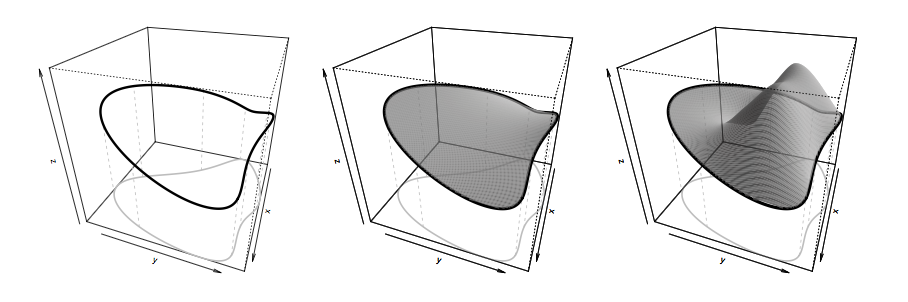
\includegraphics[width=12.61in]{images/gam_soapfilmsmoothing} 

}

\caption{Soap film smoothing 설명 그림.}\label{fig:unnamed-chunk-209}
\end{figure}

\(n\)개의 자료가 \(z_{k}\)가 있고 이것이 \(h(x_{k},y_{k})\)의 잡음이 있는 관찰값들이라고 할 때(물론 \(h\)는 정의역에서 부드러운 함수라고 가정한다), 우리는 \(h\)를 다음 조건을 최소화 하는 것으로 추정하려고 한다.
\begin{equation}
\sum_{i=1}^{n}\{ z_{i}-f(x_{i},y_{i})\}^{2}+\lambda J_{\Omega}(f).
\label{eq:soapfilmsmoothing}
\end{equation}

여기서 \(\lambda\)는 tunable smoothing parameter이다. 이 추정문제는 동기는 달랐지만 \citep{Ramsay2002}에서 처음 다뤘다. \citep{Ramsay2002}는 유한요소법을 활용한 fitting method를 제시했으나 이 방법은 단순한 형태의 basis-penalty representation을 제시하지는 못한다.

\hypertarget{--tensor-product-smooth-interactions}{%
\section{텐서곱 스므딩 상호효과들(tensor product smooth interactions)}\label{--tensor-product-smooth-interactions}}

\citep{Wood2006} 내용의 5장을 참고한다. 위에서 제시한 smoothing 방법들은 smooths의 isotropy를 가정하고 진행한다. 그러나 이런 방법은 몇 가지 단점들이 존재한다. 그 중 가장 대표적인 단점은 똑같은 smoothness를 주기 위해 어느정도로 스케일링하여 맞춰야할 지 알아맞추기 힘들다는 것이다. 예를 들어, 1차원 공간 좌표와 1차원 시간 좌표를 갖고 있는 자료를 다룰 때 단위가 m, hour 등으로 다르므로 시간의 부드러움과 공간의 부드러움의 상대적 중요도를 나타내는 것은 매우 어려운 일일 것이다.

\hypertarget{-tensor-product-bases}{%
\subsection{텐서곱 기저들(tensor product bases)}\label{-tensor-product-bases}}

이 과정(process)는 각 공변량들 \(f_{x}\), \(f_{z}\), \(f_{v}\)에 대해 부드러운 함수를 낮은 차원의 기저로 표현할 수 있다고 가정하는 데에서 부터 시작한다. 따라서 다음과 같이 쓸 수 있다.

\[f_{x}(x)=\sum_{i=1}^{I}\alpha_{i}a_{i}(x), f_{z}(z)=\sum_{l=1}^{L}\delta_{l}d_{l}(z), f_{v}(v)=\sum_{k=1}^{K}\beta_{k}b_{k}(v).\]
여기서 \(\alpha_{i}\), \(\delta_{i}\), \(\beta_{i}\)는 모수들이며 \(a_{i}(x)\), \(d_{i}(z)\), \(b_{k}(v)\)는 알려진 기저함수들이다.

이제는 \(x\)의 부드러운 함수 \(f_{x}\)가 어떻게 \(x\)와 \(z\)의 부드러운 함수로 변환될 수 있는지 생각해보자.

\hypertarget{ts}{%
\chapter{시계열분석}\label{ts}}

내용과 표기는 \citep{Shumway2010}를 따른다. \citep{Cryer2008}또한 R 예제가 이쓴 시계열분석 교재로써 참고할 만 하다.

시계열에서 다루는 대부분의 확률모형들은 확률과정을 설명하는 모형이라고 한다. 관측된 시계열은 표본공간의 각 원소에 대응하는 확률과정 \(\{ Z_{t}(\omega), t=1,2,\ldots \}\)의 관측값으로 시간의 함수이며, 이를 확률과정의 \textbf{실현값(realization)} 또는 \textbf{표본통로(sample path)}라고 부른다. 우리가 과거로 돌아갈 수 있어 반복 관측을 할 수 있다면 현재 관측된 시계열은 무한히 많은 관측 가능한 확률변수들의 모임 중에서 특별히 실현된 하나에 해당된다. 시계열 분석의 가장 큰 특징은 분석의 대상이 되는 자료가 반복 관측될 수 없다는 점이다.

\hypertarget{stationary-time-series}{%
\section{정상시계열(stationary time series)}\label{stationary-time-series}}

다음 설명은 \href{http://www.dodomira.com/2016/04/21/r-시계열-분석-arima/?subscribe=success\#blog_subscription-2}{DODOMIRA}에서 따온 것이다.

안정적인 시계열이란 다음 세 가지 특징을 가진 시계열을 말한다.

\begin{enumerate}
\def\labelenumi{\arabic{enumi}.}
\tightlist
\item
  시간의 추이와 관계 없이 평균이 불변한다.
\end{enumerate}

\begin{figure}

{\centering 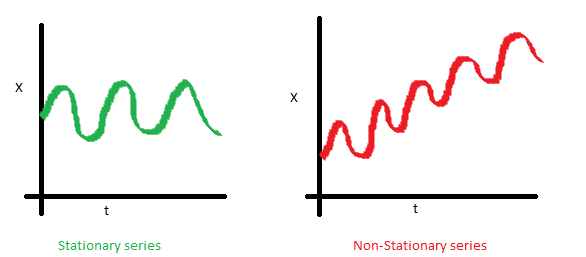
\includegraphics[width=8.14in]{images/basic_mean_nonstationary} 

}

\caption{Time invariant mean.}\label{fig:unnamed-chunk-210}
\end{figure}

\begin{enumerate}
\def\labelenumi{\arabic{enumi}.}
\setcounter{enumi}{1}
\tightlist
\item
  시간의 추이와 관계 없이 분산이 불변한다.
\end{enumerate}

\begin{figure}

{\centering 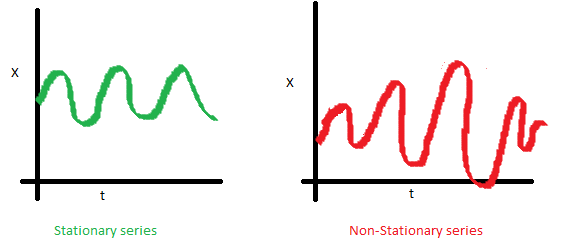
\includegraphics[width=8.01in]{images/basic_var_nonstationary} 

}

\caption{Time invariant variance.}\label{fig:unnamed-chunk-211}
\end{figure}

\begin{enumerate}
\def\labelenumi{\arabic{enumi}.}
\setcounter{enumi}{2}
\tightlist
\item
  시간의 추이와 관계 없이 공분산이 불변한다.
\end{enumerate}

\begin{figure}

{\centering 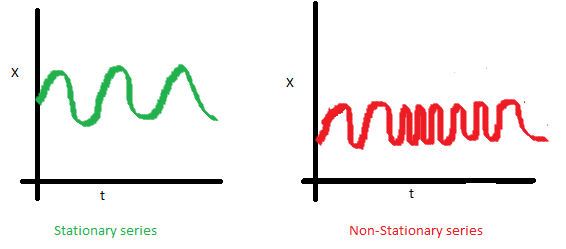
\includegraphics[width=7.86in]{images/basic_cov_nonstationary} 

}

\caption{Time invariant covariance.}\label{fig:unnamed-chunk-212}
\end{figure}

\BeginKnitrBlock{definition}[강정상성]
\protect\hypertarget{def:unnamed-chunk-213}{}{\label{def:unnamed-chunk-213} \iffalse (강정상성) \fi{} }시계열 \(\{ x_{t}\}\)가 있을 때 두 collection

\[\{ x_{t_{1}}, x_{t_{2}}, \cdots  x_{t_{k}}\}, \{ x_{t_{1+h}}, x_{t_{2+h}}, \cdots  x_{t_{k+h}}\}\]

가 identical하다면, 즉 모든 \(k=1,2,\ldots\), 모든 숫자 \(c_{1},c_{2},\ldots , c_{k}\) 그리고 \(h=0, \pm 1, \pm 2,\ldots\)에 대해

\[P \{ x_{t_{1}} <c_{1}, \ldots , x_{t_{k}} \leq c_{k}\}=P \{ x_{t_{1+h}} <c_{1}, \ldots , x_{t_{k+h}} \leq c_{k}\}\]

일 때 이 시계열을 \textbf{강정상성(strictly stationary)}이라고 한다.
\EndKnitrBlock{definition}

\citep{Huser2013}에 따르면 강정상성은 translation이 그 과정의 확률적 성질에 영향을 미치지 않는 것을 의미한다. 다시 말하면 변수들이 상호 관련있는 수열이라고 하더라도 그것의 확률적 성질들은 시간에 따라 동일한 것이다.

그러나 강정상성의 정의는 대부분의 응용에서 너무 강한 조건인데, 특히 single data set으로부터 강정상성을 assess하기 어렵다고 한다. 시계열에서는 series의 첫 두 moment에만 관련된 약정상성을 생각하여 조건을 부드럽게 한다. \citep{Huser2013}에 따르면 강정상성과 달리 약정상성은 처음 2개의 모멘트에서만 temporal homogeneity가 성립함을 가정하는 것이다.

\BeginKnitrBlock{definition}[약정상성]
\protect\hypertarget{def:unnamed-chunk-214}{}{\label{def:unnamed-chunk-214} \iffalse (약정상성) \fi{} }시계열 \(x_{t}\)가 finite variance를 갖는 process이며

\begin{enumerate}
\def\labelenumi{\arabic{enumi}.}
\item
  평균함수 \(\mu_{t}\)가 상수이며 시간에 따라 변하지 않고
\item
  자기공분산함수 \(\gamma(s,t)\)가 이들의 차이 \(|s-t|\)에만 depend할 때
\end{enumerate}

이 시계열을 \textbf{약정상성(weekly stationary)}이라고 한다.
\EndKnitrBlock{definition}

비정상 시계열 자료는 다루기 어려우므로 보통 분석하기 쉬운 정상성 시계열 자료로 변환해서 분석한다.

\BeginKnitrBlock{definition}[자기공분산함수]
\protect\hypertarget{def:unnamed-chunk-215}{}{\label{def:unnamed-chunk-215} \iffalse (자기공분산함수) \fi{} }정상시계열의 \textbf{자기공분산함수(autocovariance function)}는
\[\gamma(h)=Cov(x_{t+h}, x_{t})=E[(x_{t+h}-\mu)(x_{t}-\mu)]\]
로 정의된다.
\EndKnitrBlock{definition}

\BeginKnitrBlock{definition}[자기상관함수]
\protect\hypertarget{def:unnamed-chunk-216}{}{\label{def:unnamed-chunk-216} \iffalse (자기상관함수) \fi{} }정상시계열의 \textbf{자기상관함수(autocorrelation function)}는
\[\rho(h)=\frac{\gamma(t+h,t)}{\sqrt{\gamma(t+h,t_h)\gamma(t,t)}}=\frac{\gamma(h)}{\gamma(0)}\]
이다. 이는 \(h\) 기간 떨어진 값들의 상관계수를 의미한다. 특별히 서로 다른 두 시점의 중간에 있는 값들의 영향을 제외시킨 상관계수를 \textbf{부분자기상관함수(partial ACF)}라고 부른다.
\EndKnitrBlock{definition}

\begin{itemize}
\item
  linear process, guassian process
\item
  ACF, PACF, CCF
\end{itemize}

\hypertarget{-characteristics-of-time-series}{%
\section{시계열자료의 특성(characteristics of time series)}\label{-characteristics-of-time-series}}

\hypertarget{-time-series-regression}{%
\section{시계열 회귀분석(time series regression)}\label{-time-series-regression}}

회귀분석 모형은 시간 영역 모형과 주파수 영역 모형에서 모두 중요한 역할을 한다. 만약 \(x_{t}\)를 \(x_{t-1}, \ldots, x_{t-p}\)의 선형결합으로 표현한다면 이것은 시간 영역에의 응용이 된다. 물론 일반적인 시계열 분석에서는 회귀분석과 달리 설명변수에 해당하는 \(x_{t-1}, \ldots, x_{t-p}\)들 또한 무작위라는 차이점이 있다.
만약 우리가 사인, 코사인 함수를 투입값으로 둔다면, 주파수 영역의 아이디어는 피리오도그램과 스펙트럼을 이끌어내고 이것은 회귀모형으로부터 얻어진다. 필터를 무한한 정도로 확장하면 주파수 영역에서의 회귀분석을 다룰 수 있다. 실제로, 주파수 영역에서의 많은 회귀분석 문제들은 투입과 산출 함수들을 주기 성분의 함수들로 나타는 것이다.

\(x_{t},t=1,\ldots ,n\)을 시계열 자료라고 하자. 그리고 이 자료가 다른 투입량 또는 독립적인 시계열 \(z_{t1}, z_{t2}, \ldots ,z_{tq}\)의 영향을 받는다고 하자. 이 가정은 일반적인 회귀분석에서 놓는 가정이다. 이 관계를 회귀분석 모형으로 쓰면
\begin{equation}
x_{t}=\beta_{1}z_{t1}+\beta_{2}z_{t2}+\ldots + \beta_{q}z_{tq}+w_{t}
\label{eq:tsreg}
\end{equation}
로 놓을 수 있다. 이 때 \(\beta_{1},\beta_{2}.\ldots , \beta_{q}\)는 알려지지 않은 고정된 회귀계수(regression coefficients)들이고 \(\{ w_{t}\}\)는 i.i.d. 정규분포\((0,\sigma_{w}^{2})\)를 따르는 무작위 오류나 잡음과정(noise process)이라고 놓는다.

선형모형 \eqref{eq:tsreg}은 일반적으로 벡터 \(\mathcal{z}_{t}=(z_{t1},z_{t2},\ldots , z_{tq})^{T}\), \(\boldsymbol{\beta}(\beta_{1},\beta_{2},\ldots ,\beta_{q})^{T}\)를 써서 나타낸다. 그러면 (\eqref{eq:tsreg})은
\begin{equation}
x_{t}=\boldsymbol{\beta}^{T}\mathcal{z}_{t}+w_{t}
\label{eq:tsregvec}
\end{equation}
으로 간단히 쓸 수 있다. 이 때 알려지지 않은 모수 \(\boldsymbol{\beta}\)의 추정은 다음 식
\begin{equation}
Q=\sum_{t=1}^{n}w_{t}^{2}=\sum_{t=1}^{n}(x_{t}-\boldsymbol{\beta}^{T}\mathbf{z}_{t})^{2}
\label{eq:tsss}
\end{equation}
를 \(\beta_{1},\beta_{2},\ldots ,\beta_{q}\)에 대해 풀어 얻을 수 있다.

다시 식 \eqref{eq:tsreg}를 행렬 형태로 바꿔서 풀어보자. \(n\times q\) 행렬 \(Z= [\mathbf{z}_{1} | \mathbf{z}_{2} | \cdots | \mathbf{z}_{n} ]^{T}\)과 \(n \times 1\) 벡터 \(\mathcal{x}=(x_{1},x_{2},\ldots , x_{n})^{T}\), \(n \times 1\) 오차의 벡터 \(\mathcal{w}=(w_{1},w_{2}, \ldots, w_{n})^{T}\)를 이용해 식 \eqref{eq:tsss}를
\begin{equation}
\mathbf{x}=Z\boldsymbol{\beta}+\mathbf{w}
\label{eq:tsmatrix}
\end{equation}
로 바꿔 쓸 수 있다. 이것을 \textbf{정규방정식(normal equation)}이라고 쓴다. (\eqref{eq:tsmatrix})의 해는 \(Z^{T}Z\)이 nonsingular일 때

\[\hat{\boldsymbol{\beta}}=(Z^{T}Z)^{-1}Z^{T}\mathbf{x}\]

로 얻을 수 있다.

오차 \(w_{t}\)가 정규분포를 따르면, \(\hat{\boldsymbol{\beta}}\)는 \(\beta\)의 최대가능도추정량(maximum likelihood estimator)을 따르며

\[Cov(\hat{\boldsymbol{\beta}})=\sigma_{w}^{2}(\sum_{t=1}^{n}\mathbf{z}_{t}\mathbf{z}_{t}^{T})^{-1}=\sigma_{w}^{2}(Z^{T}Z)^{-1}=\sigma_{w}^{2}C\]

이다. 여기서

\[C=(Z^{T}Z)^{-1}\]

은 나중에 식을 전개하기 위해 미리 정의해 둔다.

선형 예측을 위해 많이 쓰는 \textbf{사영 정리(projection theorem)}을 여기에 적어둔다.

\BeginKnitrBlock{theorem}[사영 정리]
\protect\hypertarget{thm:projectiontheorem}{}{\label{thm:projectiontheorem} \iffalse (사영 정리) \fi{} }\(\mathcal{M}\)이 힐버트 공간 \(\mathcal{H}\)의 닫힌 부분 공간이고 \(y\)는 \(\mathcal{H}\)의 원소라고 하자. 그러면 \(y\)는
\begin{equation}
y=\hat{y}+z
\end{equation}
로 유일하게 표현할 수 있다. 이 때 \(\hat{y}\)는 \(\mathcal{M}\)에 속하며 \(z\)는 \(\mathcal{M}\)과 직교한다. 즉, 모든 \(w\in\mathcal{M}\)에 대해 \(\langle z,w \rangle=0\)이다. 더불어 점 \(\hat{y}\)는 \(y\)와 가장 가까운 점이다. 이 말인 즉슨, 모든 \(w\in\mathcal{M}\)에 대해 \(\| y-w\|\geq \|y-\hat{y}\|\)이고 등호는 \(w=\hat{y}\)일 때 성립한다는 말이다.
\EndKnitrBlock{theorem}

\hypertarget{differencing}{%
\section{차분(differencing)}\label{differencing}}

시계열 자료가 정상성(stationary)을 유지하기 위해서 인접한 시간들에 있는 값들의 차이를 활용하는 경우가 많다. 왜냐면 이는 자기상관(autocorrelation)과도 관련이 있기 때문이다.

\begin{Shaded}
\begin{Highlighting}[]
\KeywordTok{library}\NormalTok{(astsa)}
\NormalTok{fit =}\StringTok{ }\KeywordTok{lm}\NormalTok{(gtemp}\OperatorTok{~}\KeywordTok{time}\NormalTok{(gtemp), }\DataTypeTok{na.action=}\OtherTok{NULL}\NormalTok{) }\CommentTok{# regress gtemp on time}
\KeywordTok{par}\NormalTok{(}\DataTypeTok{mfrow=}\KeywordTok{c}\NormalTok{(}\DecValTok{2}\NormalTok{,}\DecValTok{1}\NormalTok{))}
\KeywordTok{plot}\NormalTok{(}\KeywordTok{resid}\NormalTok{(fit), }\DataTypeTok{type=}\StringTok{"o"}\NormalTok{, }\DataTypeTok{main=}\StringTok{"detrended"}\NormalTok{)}
\KeywordTok{plot}\NormalTok{(}\KeywordTok{diff}\NormalTok{(gtemp), }\DataTypeTok{type=}\StringTok{"o"}\NormalTok{, }\DataTypeTok{main=}\StringTok{"first difference"}\NormalTok{)}
\end{Highlighting}
\end{Shaded}

\begin{figure}

{\centering 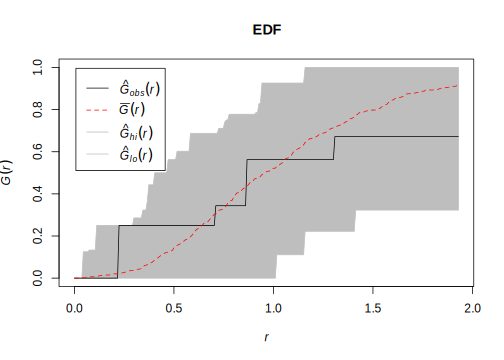
\includegraphics{book_files/figure-latex/unnamed-chunk-217-1} 

}

\caption{Detrended (top) and differenced (bottom) global temperature series.}\label{fig:unnamed-chunk-217}
\end{figure}

\begin{Shaded}
\begin{Highlighting}[]
\KeywordTok{par}\NormalTok{(}\DataTypeTok{mfrow=}\KeywordTok{c}\NormalTok{(}\DecValTok{3}\NormalTok{,}\DecValTok{1}\NormalTok{)) }\CommentTok{# plot ACFs}
\KeywordTok{acf}\NormalTok{(gtemp, }\DecValTok{48}\NormalTok{, }\DataTypeTok{main=}\StringTok{"gtemp"}\NormalTok{)}
\KeywordTok{acf}\NormalTok{(}\KeywordTok{resid}\NormalTok{(fit), }\DecValTok{48}\NormalTok{, }\DataTypeTok{main=}\StringTok{"detrended"}\NormalTok{)}
\KeywordTok{acf}\NormalTok{(}\KeywordTok{diff}\NormalTok{(gtemp), }\DecValTok{48}\NormalTok{, }\DataTypeTok{main=}\StringTok{"first difference"}\NormalTok{)}
\end{Highlighting}
\end{Shaded}

\begin{figure}

{\centering 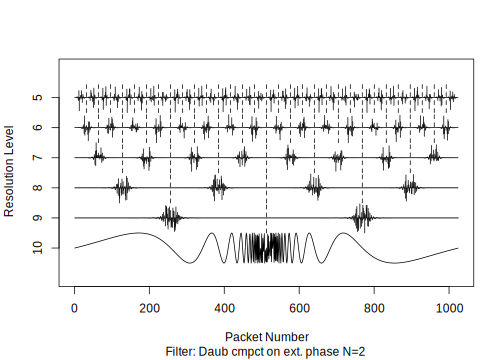
\includegraphics{book_files/figure-latex/unnamed-chunk-218-1} 

}

\caption{Sample ACF (top) detrended sample ACF (middle) and differenced (bottom) global temperature series.}\label{fig:unnamed-chunk-218}
\end{figure}

\hypertarget{armia-arima-models}{%
\section{ARMIA 모델들(ARIMA models)}\label{armia-arima-models}}

\hypertarget{ar-ar-models}{%
\subsection{AR 모형(AR models)}\label{ar-ar-models}}

이 모형은 현재의 관측값을 과거의 관측값들의 함수형태로 나타내는 것이다.

\BeginKnitrBlock{definition}[자기회귀모형]
\protect\hypertarget{def:unnamed-chunk-219}{}{\label{def:unnamed-chunk-219} \iffalse (자기회귀모형) \fi{} }\textbf{AR(p)} 차수 p를 갖는 \textbf{자기회귀모형(autoregressive model, AR model)}은
\[x_{t}=\phi_{1}x_{t-1}+\phi_{2}x_{t-2} + \cdots + \phi_{p}x_{t-p}+w_{t}\]
와 같은 형태를 갖는다. 여기서 \(x_{t}\)는 정상과정이며, \(\phi_{1},\ldots , \phi_{p}\)는 상수이다. \((\phi_{p}\neq 0)\). 그리고 \(w_{t}\)는 보통 평균이 0이고 분산이 \(\sigma_{w}^{2}\)인 백색잡음이라고 놓는다. 따로 언급하지 않으면, \(x_{t}\)의 평균은 0이라고 둔다. 만약 평균이 0이 아니고 \(\mu\)라고 할 때는 다음과 같이 \(x_{t}\) 대신 \(x_{t}-\mu\)를 사용하여
\[x_{t}-\mu = \phi_{1}(x_{t-1}-\mu)+\phi_{2}(x_{t-2}-\mu) + \cdots + \phi_{p}(x_{t-p}-\mu)+w_{t}\]
또는 \(\alpha=\mu(1-\phi_{1}-\cdots - \phi_{p})\)로 놓아
\[x_{t}=\alpha + \phi_{1}x_{t-1}+\phi_{2}x_{t-2} + \cdots + \phi_{p}x_{t-p}+w_{t}\]
\EndKnitrBlock{definition}

AR 모형이 시계열 회귀분석의 정의와 유사하므로 자기회귀(autoregression)라는 이름이 붙은 것이다. 그러나 모형을 적용하기엔 어려운데 \(x_{t-1}, \ldots, x_{t-p}\)는 무작위 요인들인데, \(\mathbf{z}_{t}\)는 고정된 요인이었기 때문이다.

일반적으로 AR과정의 ACF는 지수적으로 감소하며, PACF는 AR과정의 차수에 해당되는 차수 이후에는 0이 되는 성질을 갖고 있다.

\begin{Shaded}
\begin{Highlighting}[]
\KeywordTok{par}\NormalTok{(}\DataTypeTok{mfrow=}\KeywordTok{c}\NormalTok{(}\DecValTok{3}\NormalTok{,}\DecValTok{2}\NormalTok{))}
\NormalTok{ARsim01 <-}\StringTok{ }\KeywordTok{arima.sim}\NormalTok{(}\KeywordTok{list}\NormalTok{(}\DataTypeTok{order=}\KeywordTok{c}\NormalTok{(}\DecValTok{1}\NormalTok{,}\DecValTok{0}\NormalTok{,}\DecValTok{0}\NormalTok{), }\DataTypeTok{ar=}\NormalTok{.}\DecValTok{9}\NormalTok{), }\DataTypeTok{n=}\DecValTok{100}\NormalTok{)}
\NormalTok{ARsim02 <-}\StringTok{ }\KeywordTok{arima.sim}\NormalTok{(}\KeywordTok{list}\NormalTok{(}\DataTypeTok{order=}\KeywordTok{c}\NormalTok{(}\DecValTok{1}\NormalTok{,}\DecValTok{0}\NormalTok{,}\DecValTok{0}\NormalTok{), }\DataTypeTok{ar=}\OperatorTok{-}\NormalTok{.}\DecValTok{9}\NormalTok{), }\DataTypeTok{n=}\DecValTok{100}\NormalTok{)}
\KeywordTok{plot}\NormalTok{(ARsim01, }\DataTypeTok{ylab=}\StringTok{"x"}\NormalTok{, }\DataTypeTok{main=}\NormalTok{(}\KeywordTok{expression}\NormalTok{(}\KeywordTok{AR}\NormalTok{(}\DecValTok{1}\NormalTok{)}\OperatorTok{~}\ErrorTok{~~}\NormalTok{phi}\OperatorTok{==+}\NormalTok{.}\DecValTok{9}\NormalTok{)))}
\KeywordTok{plot}\NormalTok{(ARsim02, }\DataTypeTok{ylab=}\StringTok{"x"}\NormalTok{, }\DataTypeTok{main=}\NormalTok{(}\KeywordTok{expression}\NormalTok{(}\KeywordTok{AR}\NormalTok{(}\DecValTok{1}\NormalTok{)}\OperatorTok{~}\ErrorTok{~~}\NormalTok{phi}\OperatorTok{==-}\NormalTok{.}\DecValTok{9}\NormalTok{)))}
\KeywordTok{acf}\NormalTok{(ARsim01); }\KeywordTok{acf}\NormalTok{(ARsim02); }\KeywordTok{pacf}\NormalTok{(ARsim01); }\KeywordTok{pacf}\NormalTok{(ARsim02)}
\end{Highlighting}
\end{Shaded}

\begin{figure}

{\centering 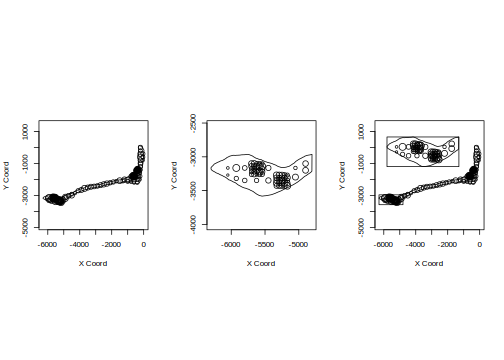
\includegraphics{book_files/figure-latex/unnamed-chunk-220-1} 

}

\caption{Simulated AR model.}\label{fig:unnamed-chunk-220}
\end{figure}

\hypertarget{ma-ma-models}{%
\subsection{MA 모형(MA models)}\label{ma-ma-models}}

AR과정과 더불어 생각해 볼 수 있는 모형으로 \textbf{이동평균모형(moving average model, MA model)}이라는 것이 있다. \(q\)차 MA 모형은 \(\text{MA}(q)\)로 보통 쓰며 백색 잡음 \(w_{t}\)가 선형결합 된 것을 관찰한다고 생각한다.

\BeginKnitrBlock{definition}[이동평균모형]
\protect\hypertarget{def:unnamed-chunk-221}{}{\label{def:unnamed-chunk-221} \iffalse (이동평균모형) \fi{} }차수 \(q\)를 갖는 \textbf{이동평균모형(moving average model)}은 다음과 같이 정의된다.
\[x_{t}=w_{t}+\theta_{1}w_{t-1}+\theta_{2}w_{t-2}+\ldots \theta_{q}w_{t-q}.\]
이때 \(w_{t}\sim \text{WM}(0,\sigma_{w}^{2})\)이며 \(\theta_{1},\ldots, \theta_{q}(\theta_{q}\neq 0)\)은 모수들이다.
\EndKnitrBlock{definition}

또한 다음과 같이 \textbf{이동평균작용소(moving average operator)}를 정의하여 식을 간단히 쓸 수 있다.

\BeginKnitrBlock{definition}[이동평균작용소]
\protect\hypertarget{def:unnamed-chunk-222}{}{\label{def:unnamed-chunk-222} \iffalse (이동평균작용소) \fi{} }\textbf{이동평균작용소(moving average operator)} \(\theta(B)\)는
\[\theta(B)=1+\theta_{1}B+\theta_{2}B^{2}+\ldots +\theta_{q}B^{q}\]
로 정의된다.
\EndKnitrBlock{definition}

이동평균작용소를 이용해 \(\text{MA}(q)\)과정을 다시쓰면 다음과 같다.
\[x_{t}=\theta(B)w_{t}.\]

\BeginKnitrBlock{example}[MA(1)과정]
\protect\hypertarget{exm:unnamed-chunk-223}{}{\label{exm:unnamed-chunk-223} \iffalse (MA(1)과정) \fi{} }MA과정 중에서 가장 간단한 모형으로 MA(1) 과정이 있으며 다음과 같이 쓴다.
\[x_{t}=w_{t}+\theta w_{t-1}.\]
그러면 \(E(x_{t})=0\)이다. 이것의 자기공분산함수는 다음과 같다.

\[
\gamma(h) = 
\begin{cases}
(1+\theta^{2})\sigma_{w}^{2} & h=0,\\
\theta \sigma_{w}^{2} & h=1,\\
0 & h>1.
\end{cases}
\]

ACF는 다음과 같다.

\[
\rho(h) = 
\begin{cases}
\frac{\theta}{(1+\theta^{2})} & h=1,\\
0 & h>1.
\end{cases}
\]

한편 모든 \(\theta\)에서 \(|\rho(1)|\leq 0.5\)이다. 그리고 \(x_{t}\)는 \(x_{t-1}\)과는 연관되어 있지만, \(x_{t-2}, x_{t-3},\ldots\)등과는 연관되어 있지 않다. 이는 \(AR(1)\)과정에서 \(x_{t}\)와 \(x_{t-k}\) 사이의 상관관계가 0이 되지 않는 것과는 대조적이다. 예를 들어 \(\theta=0.9\)일 때 \(x_{t}\)와 \(x_{t-1}\)은 양의 상관관계를 갖으며 \(\theta_{1}=0.497\)이다. 한편 \(\theta=-0.9\)일 때에는 \(x_{t}\)와 \(x_{t-1}\)은 음의 상관관계를 갖으며 \(\theta_{1}=-0.497\)이다.
\EndKnitrBlock{example}

MA과정의 PACF는 AR과정의 ACF 형태와, MA과정의 ACF는 AR과정의 PACF 형태와 같다. 참고로 유한 개의 항을 가지는 MA과정은 항상 정상과정이므로 AR과정과는 달리 유한차수의 MA과정에 대해서는 정상성 조건을 논의할 필요가 없다.

\begin{Shaded}
\begin{Highlighting}[]
\KeywordTok{par}\NormalTok{(}\DataTypeTok{mfrow=}\KeywordTok{c}\NormalTok{(}\DecValTok{3}\NormalTok{,}\DecValTok{2}\NormalTok{))   }
\NormalTok{MAsim01 <-}\StringTok{ }\KeywordTok{arima.sim}\NormalTok{(}\KeywordTok{list}\NormalTok{(}\DataTypeTok{order=}\KeywordTok{c}\NormalTok{(}\DecValTok{0}\NormalTok{,}\DecValTok{0}\NormalTok{,}\DecValTok{1}\NormalTok{), }\DataTypeTok{ma=}\NormalTok{.}\DecValTok{9}\NormalTok{), }\DataTypeTok{n=}\DecValTok{100}\NormalTok{)}
\NormalTok{MAsim02 <-}\StringTok{ }\KeywordTok{arima.sim}\NormalTok{(}\KeywordTok{list}\NormalTok{(}\DataTypeTok{order=}\KeywordTok{c}\NormalTok{(}\DecValTok{0}\NormalTok{,}\DecValTok{0}\NormalTok{,}\DecValTok{1}\NormalTok{), }\DataTypeTok{ma=}\OperatorTok{-}\NormalTok{.}\DecValTok{9}\NormalTok{), }\DataTypeTok{n=}\DecValTok{100}\NormalTok{)}
\KeywordTok{plot}\NormalTok{(MAsim01, }\DataTypeTok{ylab=}\StringTok{"x"}\NormalTok{, }\DataTypeTok{main=}\NormalTok{(}\KeywordTok{expression}\NormalTok{(}\KeywordTok{MA}\NormalTok{(}\DecValTok{1}\NormalTok{)}\OperatorTok{~}\ErrorTok{~~}\NormalTok{theta}\OperatorTok{==+}\NormalTok{.}\DecValTok{9}\NormalTok{)))    }
\KeywordTok{plot}\NormalTok{(MAsim02, }\DataTypeTok{ylab=}\StringTok{"x"}\NormalTok{,}\DataTypeTok{main=}\NormalTok{(}\KeywordTok{expression}\NormalTok{(}\KeywordTok{MA}\NormalTok{(}\DecValTok{1}\NormalTok{)}\OperatorTok{~}\ErrorTok{~~}\NormalTok{theta}\OperatorTok{==-}\NormalTok{.}\DecValTok{9}\NormalTok{))) }
\KeywordTok{acf}\NormalTok{(MAsim01); }\KeywordTok{acf}\NormalTok{(MAsim02); }\KeywordTok{pacf}\NormalTok{(MAsim01); }\KeywordTok{pacf}\NormalTok{(MAsim02)}
\end{Highlighting}
\end{Shaded}

\begin{figure}

{\centering 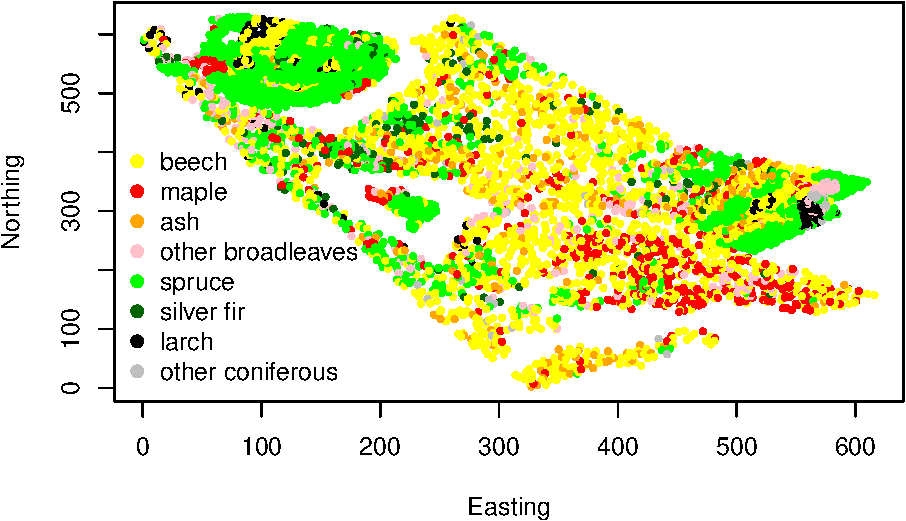
\includegraphics{book_files/figure-latex/unnamed-chunk-224-1} 

}

\caption{Simulated MA model.}\label{fig:unnamed-chunk-224}
\end{figure}

\BeginKnitrBlock{example}[유일하지 않은 MA 모형들과 가역성]
\protect\hypertarget{exm:unnamed-chunk-225}{}{\label{exm:unnamed-chunk-225} \iffalse (유일하지 않은 MA 모형들과 가역성) \fi{} }한편 \(\sigma_{w}^{2}=1\)이고 \(\theta=5\)인 MA(1) 모형은 \(\sigma_{w}^{2}=25\)이고 \(\theta=1/5\)인 MA(1) 모형과 같은 autocovariance function을 갖는다. 즉 이 때는

\[
\gamma(h) = 
\begin{cases}
26 & h=0,\\
5 \sigma_{w}^{2} & h=1,\\
0 & h>1.
\end{cases}
\]

이다. 즉 다음 두 MA(1) 과정
\[x_{t}=w_{t}+\frac{1}{5}w_{t-1}, \qquad{w_{t}\stackrel{\text{i.i.d}}{\sim}\mathcal{N}(0,25)}\]
\[y_{t}=v_{t}+5v_{t-1}, \qquad{v_{t}\stackrel{\text{i.i.d}}{\sim}\mathcal{N}(0,1)}\]
은 같은 것이다. 우리는 시계열 \(x_{t}\), \(y_{t}\)만 관찰할 수 있고 잡음들 \(w_{t}\), \(v_{t}\)은 관찰 못하므로 이들을 구분해낼 수 없다. 편의를 위해 \(x_{t}\)와 \(w_{t}\)의 역할을 바꾸면 MA(1) 모형을
\[w_{t}=-\theta w_{t-1}+x_{t}\]
로 쓸 수 있다. 이러면 AR 모형처럼 되고, \(|\theta|<1\)인 조건을 적용시키면 \(w_{t}=\sum_{j=0}^{\infty}(-\theta)^{j}x_{t-j}\)임을 알 수 있다. 따라서 여러 가지 MA 모형이 있을 경우, \textbf{가역(invertible)}한 \(\sigma_{w}^{2}=25\)이고 \(\theta=1/5\) 모형을 고르게 된다.
\EndKnitrBlock{example}

\hypertarget{arma-arma-models}{%
\subsection{ARMA 모형(ARMA models)}\label{arma-arma-models}}

비정상 시계열 모형 중 하나로, 차분이나 변환을 통해 AR, MA 또는 이 둘을 합한 ARMA 모형으로 정상화 시켜 모델링한다.

It also possible to obtain a homogeneous difference equation directly in terms of \(\gamma(h)\). First, we write

\[
\begin{eqnarray}
\gamma(h)&=&\text{cov}(x_{t+h},x_{t})\\
&=&\text{cov}(\sum_{j=1}^{p}\phi_{j}x_{t+h-j}+\sum_{j=0}^{q}\theta_{j}w_{t+h-j},x_{t})\\
&=&\sum_{j=1}^{p}\phi_{j}\gamma(h-j)+\sigma_{w}^{2}\sum_{j=h}^{q}\theta_{j}\psi_{j-h}, h \geq 0.
\end{eqnarray}
\]

general homoegeneous equations for the ACF of the ARMA process
\[\gamma(h)-\phi_{1}\gamma(h-1)-\cdots - \phi_{p}\gamma(h-p)=0, h\geq \max(p,q+1)\]

\hypertarget{arma--estimation-of-arma-models}{%
\subsubsection{ARMA 모형의 추정(estimation of ARMA models)}\label{arma--estimation-of-arma-models}}

\BeginKnitrBlock{definition}[Yule-Walker equations]
\protect\hypertarget{def:unnamed-chunk-226}{}{\label{def:unnamed-chunk-226} \iffalse (Yule-Walker equations) \fi{} }\[\gamma(h)=\phi_{1}\gamma(h-1)+\cdots +\phi_{p}\gamma(h-p), h=1,2,\ldots, p, \]
\[\sigma_{w}^{2}=\gamma(0)-\phi_{1}\gamma(1)-\cdots - \phi_{p}\gamma(p).\]

Matrix notation으로는
\[\Gamma_{p}\phi=\gamma_{p}, \sigma_{w}^{2}=\gamma(0)-\phi'\gamma_{p}\]
이며 \(\Gamma_{p}=\{ \gamma (k-j) \}_{j,k=1}^{p}\)는 \(p\times p\) 행렬이며 \(\phi=(\phi_{1},\ldots , \phi_{p})'\)는 \(p\times 1\) 벡터이며 \(\gamma(p)=(\gamma(1),\ldots ,\gamma(p))'\)는 \(p\times 1\) 벡터이다.
\EndKnitrBlock{definition}

\hypertarget{arima-arima-models}{%
\subsection{ARIMA 모형(ARIMA models)}\label{arima-arima-models}}

\hypertarget{--arima-seasonal-arima-models}{%
\section{계절성이 있는 ARIMA 모델링(seasonal ARIMA models)}\label{--arima-seasonal-arima-models}}

시계열이 일정한 계절적인 주기를 가지고 변할 때 사용하는 분석 방법으로는 삼각함수 또는 지시함수를 이용한 회귀모형, 계절형 지수평활법 등이 있다. 이러한 방법들은 계절형 시계열이
\[x_{t}=T_{t}+S_{t}+C_{t}+I_{t}\]
와 같이 서로 독립적인 여러 성분들로 구성되어 있을 때 사용 가능하다고 한다.

\begin{itemize}
\item
  \(T_{t}\): 추세성분
\item
  \(S_{t}\): 계절성분
\item
  \(C_{t}\): 순환성분
\item
  \(I_{t}\): 불규칙성분
\end{itemize}

각 성분들은 회귀분석 또는 이동평균법 등을 이용한 전통적인 분해법에 의해 분석할 수 있다. 그러나 이러한 분석법은 시계열을 구성하고 있는 성분들이 결정적이며 서로 독립이라는 가정 하에서 출발하고 있는데, 우리가 접하는 시계열들은 그 구성성분들이 확률적이거나 다른 성분들과 상관이 있는 경우가 많다. 이러한 경우에는 확률적 분석 방법인 ARIMA를 이용한 분석을 한다.

\hypertarget{coherency-section-3.9}{%
\section{Coherency (section 3.9)}\label{coherency-section-3.9}}

\textbf{결맞음(coherency)} 분석은 두 자료의 관계를 quantify하기 위해 많이들 사용한다. 신호 사이의 결맞음 추정은 중요햐며

\hypertarget{self-similar-process-1}{%
\section{Self-Similar Process}\label{self-similar-process-1}}

\hypertarget{-linear-filter}{%
\section{선형 필터(linear filter)}\label{-linear-filter}}

이 절의 내용은 \citep{Shumway2010}를 참고하였다. 이전의 많은 예제들은 시계열에서 분산 또는 파워의 분포를 선형 변환을 만듬으로써 변형시킬 수 있는 가능성에 대한 힌트를 제시했다. 여기서는 선형 필터가 시계열로부터 신호를 어떻게 뽑아내는지에 대해 설명한다. 선형 필터는 시계열 자료의 스펙트럼 특성을 변형시켜 예측 가능하게끔 한다고 한다.

선형필터는 특정화한 계수들 \(a_{j}, j=0,\pm 1, \pm 2, \ldots\)를 사용한다. 이것은 투입된 시계열 \(x_{t}\)를 다음 관계를 통해
\[y_{t}=\sum_{j=-\infty}^{\infty}a_{j}x_{t-j}, \sum_{j=-\infty}^{\infty}|a_{j}| <\infty\]
\(y_{t}\)라는 시계열로 변화시킨다. 통계 용어로 이 식은 convolution에 해당한다. 이 계수들은 특별히 \textbf{임펄스 응답 함수(impulse response function)}이라고 부른다.

\hypertarget{transfer}{%
\chapter{전이함수모형}\label{transfer}}

시차회귀분석(lagged regression)

입력시계열과 출력시계열로 사용되는 시계열 사이의 관계를 회귀모형의 형태로 표현한 것을 \textbf{전이함수(transfer function)}라고 하며, 이 떄의 모형을 \textbf{전이함수모형(transfer function model)}이라고 한다. 일반적으로 전이함수 모형은 입력시계열이 출력시계열에는 영향을 미치나 반대의 영향은 없다는 가정 하에서 사용한다. 만약 출력시계열도 입력시계열에 영향을 미치는 경우에는 전이함수 모형 대신 벡터 ARIMA 모형을 이용한 분석을 한다.

\begin{equation}
y_{t}=\sum_{j=0}^{\infty}\alpha_{j}x_{t-j}+\eta_{t}=\alpha(B)x_{t}+\eta_{t}
\label{eq:lagreg}
\end{equation}

라고 모형을 세우자. 이 때 \(x_{t-j}\)는 입력시계열, \(\eta_{t}\)는 잡음과정이 되며
\[\alpha(B)=\sum_{j=0}^{\infty}\alpha_{j}B^{j}\]
는 전이함수가 된다. 이 때 \(\alpha_{j}\)를 \textbf{충격반응가중값(impulse response weight)}이라고 부른다.

Box와 Jenkins에 따르면, \(x_{t}\)와 \(\eta_{t}\)에 ARIMA모형을 적합한다. 이 때
\[\phi(B)x_{t}=\theta(B)w_{t} \text{ and }\]
\[\phi_{\eta}(B)\eta_{t}=\theta_{\eta}(B)z_{t}\]
로 표현할 수 있다. 이 때

\begin{itemize}
\tightlist
\item
  \(w_{t},z_{t}\)는 독립이고 분산이 \(\sigma_{w}^{2}\), \(\sigma_{z}^{2}\)인 백색잡음과정이다. Box와 Jenkins는 \(\alpha_{j}, j=1,2,\ldots\)의 형태로 systematic patteren들이 관찰될 수 있고 이들을 a ratio of polynomials involving a small number of coefficients, along with a specified delay \(d\)로 표현할 수 있다고 한다. 따라서
\end{itemize}

\[\alpha(B)=\frac{\delta (B)B^{d}}{\omega(B)}\]
로 표현할 수 있고(이렇게 표현하면 추정해야 할 모수의 숫자를 줄일 수 있다고 한다), 여기서
\[\omega(B)=1-\omega_{1}B-\omega_{2}B^{2}-\cdots -\omega_{r}B^{r}\]
이며
\[\delta(B)=\delta_{0}+\delta_{1}B+\cdots +\delta_{s}B^{s}\]
들이 지시연산자가 된다. 식 (\eqref{eq:lagreg})를 정리하면
\[\tilde{y}_{t}=\frac{\phi(B)}{\theta(B)}y_{t}=\alpha(B)w_{t}+\frac{\phi(B)}{\theta(B)}\eta_{t}=\alpha(B)w_{t}+\tilde{\eta}_{t}\]
를 얻게 된다. 이 때

\begin{itemize}
\item
  \(\alpha(B)=\sum_{j=0}^{\infty}\alpha_{j}B^{j}\): 전이함수
\item
  \(\tilde{\eta}_{t}\): 변환된 잡음으로 \(w_{t}\)와 독립
\item
  \(\frac{\phi(B)}{\theta(B)}\): \textbf{선형필터(linear filter)}라 부름
\item
  \(w_{t}\): 사전백색화된 input series
\item
  \(\tilde{y}_{t}\): 변환된 output series
\end{itemize}

전이함수모형의 기본 가정은 입력시계열과 반응시계열이 모두 정상시계열이라는 것이다. 따라서 먼저 분석에 사용될 시계열들이 정상성을 갖는지 여부를 판단해야 한다.

\hypertarget{-stability-and-causality}{%
\section{안정성과 인과성(stability and causality)}\label{-stability-and-causality}}

(조신섭 교수님 책 참고)

\hypertarget{cross-covariance-function}{%
\section{교차상관함수(cross-covariance function)}\label{cross-covariance-function}}

전이함수의 형태를 식별하기 위해서는 충격반응가중값을 먼저 구해야 하는데, 이를 위해 두 개의 시계열 사이의 상관의 정도와 방향을 나타내는 교차상관함수를 이용한다.

\BeginKnitrBlock{definition}[교차상관함수]
\protect\hypertarget{def:unnamed-chunk-227}{}{\label{def:unnamed-chunk-227} \iffalse (교차상관함수) \fi{} }정상인 두 시계열 \(X_{t}\)와 \(Y_{t}\) 사이의 교차상관함수는
\[\gamma_{XY}(t)=E[(X_{t}-\mu_{X})(Y_{t+k}-\mu_{Y})], \qquad{k=0,\pm 1, \pm 2, \ldots}\]
이다. 단 모든 \(t\)에 대해 \(\mu_{X}=E[X_{t}]\), \(\mu_{Y}=E[Y_{t}]\)이다.
\EndKnitrBlock{definition}

교차상관함수의 성질 중 중요한 것은 \textbf{자기상관함수와는 달리 대칭이 아니라}는 점이다. 따라서 교차상관함수는 자기상관함수와는 달리 상관의 정도와 영향을 미치는 방향을 같이 측정한다는 점이 특징이다.

\BeginKnitrBlock{definition}[교차상관계수]
\protect\hypertarget{def:unnamed-chunk-228}{}{\label{def:unnamed-chunk-228} \iffalse (교차상관계수) \fi{} }정상인 두 시계열 \(X_{t}\)와 \(Y_{t}\) 사이의 교차상관함수는
\[\rho_{XY}(k)=Corr(X_{t},Y_{t+k})=\frac{\gamma_{XY}(k)}{\sigma_{X}\sigma_{Y}}=\frac{\gamma_{XY}(k)}{\sqrt{\gamma_{X}(0)\gamma_{Y}(0)}}\]
으로 정의한다.
\EndKnitrBlock{definition}

앞선 모형에서 \(\tilde{y}_{t}\)와 \(w_{t}\)의 교차상관계수는
\[\gamma_{\tilde{y} w}(h)=E[\tilde{y}_{t} w_{t}]=E[\sum_{j=0}^{\infty}\alpha_{j}w_{t+h-j}w_{t}]=\sigma_{w}^{2}\alpha_{h}\]
로 쓸 수 있다. 이는 \(j=h\)일 때를 제외하고 백색잡음의 ACF가 0임을 이용하는 것이다. 이 관계식을 보면
\[\hat{\alpha}_{h}=\frac{\hat{\gamma}_{\tilde{y}w}(h)}{\hat{\sigma}_{w}^{2}}\]
임을 유추해 낼 수 있다.

\hypertarget{-fitting-transfer-function-model}{%
\section{전이함수모형의 적합(fitting transfer function model)}\label{-fitting-transfer-function-model}}

\begin{enumerate}
\def\labelenumi{\arabic{enumi}.}
\item
  먼저 분석에 이용될 시계열들이 정상이라는 가정을 만족하도록 정상화한다.
\item
  전이함수모형의 식별을 위해 시계열을 사전백색화(prewhitening)한다.
\item
  잠정적인 전이함수모형을 추정한다.
\item
  장차를 이용하여 오차모형을 식별하고 추정한다.
\end{enumerate}

\hypertarget{kalman}{%
\chapter{칼만 필터}\label{kalman}}

자연계에서 나타나는 시계열은 많은 경우, 직전의 상태와 밀접하 관계를 갖으면서 끊임없이 변화하는 형태를 보이고 있어 선형모형으로는 예측의 정확도를 높이는 데 한계가 있을 때가 있다. 실제와 닮은 모형이 더 우수하다는 원칙에서 동적모형에 대한 연구와 적용이 예보의 정확성을 높여줄 것이다.

\textbf{칼만필터(kalman filter)}란 공정제어를 위해 칼만(Kalman)이 1960년 제안한 알고리즘으로, 시간의 흐름에 따라 모형식이 변화하는 동적 모형(dynamic model)으로 선형과 비선형의 중간 형태를 지니고 있다고 한다. 예측 문제도 해결하는 등 여러 가지 장점이 있어 경제 에측, 신호 처리, 기상 예보 등 응용 범위가 넓은 동적 모형이라고 한다.

칼만 필터 모형은 다음의 생성 구조로 이루어진다.

\begin{enumerate}
\def\labelenumi{\arabic{enumi}.}
\item
  초기치가 필요하다.
\item
  주어진 \textbf{상태방정식(state equation)}에 의해 전 상태로부터 내적오차와 합하여 현 상태값이 결정되며,
\item
  주어진 \textbf{출력방정식(output equation)}에 의해 고려된 입력변수값과 동적회귀계수 역할을 하는 현 상태의 내적과 출력오차의 합 형태로 관측치가 생성된다는 가정 아래 구성된 모형으로,
\item
  새로운 관측치가 얻어지면, 모형이 \textbf{최신화(updating)}되도록 알고리즘이 주어져야 한다.
\end{enumerate}

\(F_{t}\), \(G_{t}\), \(W\), \(V\), \(m_{0}\), \(C_{0}\), \(t=1,2,\ldots,\) 가 주어진 경우 다음의 생성식으로 이루어진 모형식을 칼만필터 모형이라고 한다.

\[\text{(초기 분포) } \theta_{0} \sim \mathcal{N}(m_{0},C_{0})\]
\[\text{(상태방정식) } \theta_{t}=G_{t}\theta_{t-1}+w_{t}, \qquad{w_{t} \sim \mathcal{N}(0,W)}\]
\[\text{(출력방정식) } Y_{t}=F_{t}\theta_{t}+v_{t}, \qquad{v_{t}\sim \mathcal{N}(0,V)}\]

여기에서

\begin{itemize}
\item
  \(\theta_{t}\): \textbf{상태벡터(state vector)}
\item
  \(G_{t}\): \textbf{전이행렬(transition matrix)}
\item
  \(w_{t}\): \textbf{내적오차벡터(innovational error vector)}
\item
  \(Y_{t}\): \textbf{관측치(observation)}
\item
  \(F_{t}\): \textbf{입력벡터(input vector)}로 상태벡터가 관측치에 영향을 주는 설명변수들로 이루어져있음
\item
  \(v_{t}\): \textbf{출력오차(output error)}
\end{itemize}

\(\theta_{t-1}\)과 \(w_{t}\)는 독립이며, \(\theta_{t}\)는 \(v_{t}\)와 독립이고, 두 오차는 서로 독립이다.

칼만필터 모형은 두 개 이상의 선형식의 모임으로 연결되어 있으므로 전체적으로는 비선형적 특성을 지니고 있고, 각 식은 선형모형이므로 모형의 설명력과 예측력이 우수하며, 이론적 전개가 용이하다.

\BeginKnitrBlock{example}[칼만필터 모형의 예]
\protect\hypertarget{exm:unnamed-chunk-229}{}{\label{exm:unnamed-chunk-229} \iffalse (칼만필터 모형의 예) \fi{} }시간에 따라 생성되는 종속변수가 하나이며 설명변수가 두 개인 선형모형을 생각해보자.

\begin{enumerate}
\def\labelenumi{\arabic{enumi}.}
\item
  회귀모형은 회귀계수가 미지의 상수인 경우로 정적 모형이다. 즉
  \[Y_{t}=m_{0}+m_{1}X_{1t}+m_{2}X_{2t}+v_{t}\]
  인 형태가 된다.
\item
  회귀동적모형은 회귀계수가 시간에 따라 변화하는 경우로 동적모형이다. 즉
  \[Y_{t}=m_{0t}+m_{1t}X_{1t}+m_{2t}X_{2t}+v_{t}\]
  인 형태가 되며 각 회귀계수들을 함수형태로 추정해 주어야 한다.
\item
  회귀동적선형모형은 회귀계수가 전 시점의 회귀계수에 의하여 결정되는 경우로 회귀동적모형의 특수한 경우가 된다. 예를 들어, 전이행렬이 단위행렬인 경우(상태벡터가 임의보행인 경우)
  \[Y_{t}=m_{0t}+m_{1t}X_{1t}+m_{2t}X_{2t}+v_{t}\]
\end{enumerate}

그리고

\[
\theta_{t} =
 \begin{pmatrix}
  m_{0t} \\
  m_{1t} \\
  m_{2t} 
 \end{pmatrix}
= 
 \begin{pmatrix}
  1 & 0 & 0 \\
  0 & 1 & 0 \\
  0 & 0 & 1
 \end{pmatrix}
 \begin{pmatrix}
  m_{0,t-1} \\
  m_{1,t-1} \\
  m_{2,t-1} 
 \end{pmatrix} 
+
 \begin{pmatrix}
  w_{0t} \\
  w_{1t} \\
  w_{2t} 
 \end{pmatrix}
\]
이와 같은 형태를 지닌다.
\EndKnitrBlock{example}

\hypertarget{--types-of-kalman-filter}{%
\section{칼만필터 모형의 종류(types of Kalman filter)}\label{--types-of-kalman-filter}}

\hypertarget{--hidden-markov-model}{%
\subsection{은닉 마르코프 모형(hidden Markov model)}\label{--hidden-markov-model}}

오차항이 없는 칼만필터 모형으로 다음과 같다.

\[
\begin{cases}
\mu_{t}=G\mu_{t-1} \\
Y_{t}=F\mu_{t}.\\
\end{cases}
\]

여기서 전이행렬 \(G\)와 출력행렬 \(F\)는 시간에 따라 변화하지 않으므로 상태방정식은 확률과정에서의 상태벡터 \(\mu_{t}\)의 전이행렬이 \(G\)인 마르코프 연쇄로 생각할 수 있다. 관측치 \(Y_{t}\)만 주어져 있고 \(\mu_{t}\)는 모르는 경우 모수 \(G\)와 \(F\)를 추정하여 생성구조를 완성하는 과정을 이룬다. 은닉 마르코프 모형은 범주형 자료에도 적용이 가능하며, 신호처리에 바탕을 두고 있는 음성인식, 영상인식, 문장인식에 널리 사용되고 있는 통계적 기법이다.

\hypertarget{--simple-kalman-filter-model}{%
\subsection{일차 칼만필터 모형(simple Kalman filter model)}\label{--simple-kalman-filter-model}}

\textbf{일차 칼만필터 모형(simple Kalman filter model)}은 오차항을 포함한 칼만필터 모형 중 가장 간단한 형태로 \(t\) 시점의 상태열이 임의보행과정(random walk)으로 직전 상태값 주위에서 흔들리며 변화할 때 사용한다.

\[
\begin{cases}
\mu_{t}=\mu_{t-1}+w_{t} \\
Y_{t}=\mu_{t}+v_{t}.\\
\end{cases}
\]

\hypertarget{--regression-kalman-filter-model}{%
\subsection{회귀 칼만필터 모형(regression Kalman filter model)}\label{--regression-kalman-filter-model}}

\textbf{회귀 칼만필터 모형(regression Kalman filter model)}은 입력변수(설명변수)가 있는 경우에 사용하는 동적모형으로 계수(상태열)가 시간에 따라 변화하는 동적 계수가 된다.

\[
\begin{cases}
\theta_{t}=\theta_{t-1}+w_{t} \\
Y_{t}=F_{t}\theta_{t}+v_{t}.\\
\end{cases}
\]

\hypertarget{--general-kalman-filter-model}{%
\subsection{일반적 칼만필터 모형(general Kalman filter model)}\label{--general-kalman-filter-model}}

\textbf{일반적 칼만필터 모형(general Kalman filter model)}은 회귀 칼만필터 모형에서 동적 계수가 임의보행이 아닌 경우에 전이행렬을 고려하는 동적모형이다.

\[
\begin{cases}
\theta_{t}=G_{t}\theta_{t-1}+w_{t} \\
Y_{t}=F_{t}\theta_{t}+v_{t}.\\
\end{cases}
\]

\hypertarget{--extended-kalman-filter-model}{%
\subsection{확장된 칼만필터 모형(extended Kalman filter model)}\label{--extended-kalman-filter-model}}

칼만필터 모형에서 상태방정식과 출력방정식이 선형모형이 아닌 비선형모형인 경우를 \textbf{확장된 칼만필터 모형(extended Kalman filter model)}이라고 한다. 추정과 최시노하는 주어진 식을 선형화하여 해결하며, 시스템에 대한 물리적 이해가 필요하다.

\[
\begin{cases}
\theta_{t}=f(\theta_{t-1},w_{t}) \\
Y_{t}=h(\theta_{t},v_{t})\\
\end{cases}
\]

\hypertarget{-updating-algorithm}{%
\section{최신화 알고리즘(updating algorithm)}\label{-updating-algorithm}}

\textbf{칼만필터링(Kalman filtering)}은 칼만필터 모형의 상태열 \(\{ \theta_{t}\}\)의 추정에 사용된다. 칼만필터링은 다음의 특징을 지니고 있어 이공계 분야 모델링에 많이 응용된다.

\begin{itemize}
\item
  미지의 상태열 \(\{\theta_{t}\}\)를 추정하는 반복처리과정이다.
\item
  동적처리기법이다. 즉 시간의 흐름에 따라 진행하면서 과거와 현재의 출력값들을 보고 현재의 상태를 추정해간다.
\item
  평균제곱오차를 최소로 하는 최적 상태열을 추정하는 통계적 이론을 바탕으로 한다.
\item
  체계적 기법(systematic method)이다. 즉 일단 칼만필터 모형이 만들어지면 칼만필터 알고리즘을 쉽게 사용할 수 있다.
\item
  나쁜 초기치의 영향이 오래가지 않는다. 즉 로버스트하다.
\item
  프로그래밍이 쉽다.
\end{itemize}

칼만필터링은 다변량 정규분포이론에 근거하며 최적 상태값을 추정하는 아래와 같은 \textbf{동적순환과정(dynamic recursive procedure)}으로 이루어진다. 이를 \textbf{최신화 알고리즘(updating algoritm)}이라고 한다. \(t=1,2,\ldots\)로 변화시키며

\begin{enumerate}
\def\labelenumi{\arabic{enumi}.}
\item
  \(t-1\)시점까지의 모든 정보 \(D_{t}\)에 의한 \(\theta_{t-1}\)의 분포
  \[\theta_{t-1}|Y_{t-1} \sim \mathcal{N}(m_{t-1},C_{t-1})\]
\item
  \(t\)시점에서의 \(\theta_{t}\)의 사전분포: 상태방정식 \(\theta_{t}=G_{t}\theta_{t-1}+w_{t}, w_{t} \sim \mathcal{N}(0,W_{t})\)에 의하여,
  \[\theta_{t}|D_{t-1} = (G_{t}\theta_{t-1}+w_{t})|D_{t-1}\sim \mathcal{N}(a_{t},R_{t})\]
  여기에서 \(a_{t}=G_{t}m_{t-1}, R_{t}=G_{t}C_{t-1}G_{t}'+W_{t}\)이다.
\end{enumerate}

\hypertarget{dynamic-linear-model}{%
\section{동적선형모형(dynamic linear model)}\label{dynamic-linear-model}}

\hypertarget{r-r-dlm}{%
\section{R-예제(R-dlm)}\label{r-r-dlm}}

\hypertarget{spectral}{%
\chapter{스펙트럼 분석}\label{spectral}}

이 절의 내용은 \citep{Shumway2010}를 참고하였다.

시간영역의 분석 방법이 자기상관함수 등을 이용해 시간에 따른 상관 정도를 분석하고 변수들 사이의 관계를 가장 잘 설명해 주는 모형을 찾는 데 반해, 진동수영역의 분석 방법은 시계열이 다양한 주기를 갖는 성분들(주로 싸인과 코싸인)의 선형결합으로 표현될 수 있다는 성질을 이용해 어떤 주기성분이 중요한 역할을 하는지 알아보는 데 초점을 둔다.

진동수영역의 분석에서는 자기공분산의 \textbf{푸리에변환(Fourier transform)}으로 정의되는 \textbf{스펙트럼(spectrum)}을 추정하여 각 진동수에 대응되는 주기성분들의 선형결합으로 시계열을 표현한다. 즉, 시계열이 긴 주기 또는 짧은 주기를 갖는지를 각 주기성분들의 기여도를 이용하여 설명 및 분석하는 데, 이 기여도를 자기공분산의 형태로 표현하는 것이 \textbf{스펙트럼분석(spectral analysis)}이다.

\hypertarget{---complex-valued-stationary-time-series}{%
\section{복소수값을 갖는 정상 시계열(complex-valued stationary time series)}\label{---complex-valued-stationary-time-series}}

이 부분만은 특별히 Dewei Wang의 시계열 분석 강의노트 내용을 따랐다. 따라서 표기가 다를 수 있다.

\BeginKnitrBlock{definition}[복소수값을 갖는 정상 시계열]
\protect\hypertarget{def:unnamed-chunk-231}{}{\label{def:unnamed-chunk-231} \iffalse (복소수값을 갖는 정상 시계열) \fi{} }과정 \(\{X_{t}\}\)는 \(E|X_{t}|^{2}<\infty\)이고 \(EX_{t}\)는 \(t\)에 독립이며 \(E(X_{t+h}\bar{X}_{t})\) 또한 \(t\)에 독립일 경우 \textbf{복소수값을 갖는 정상 시계열(complex-valued stationary process)}라고 부른다. 이것의 자기공분산 함수 \(\gamma_{X}(\cdot)\)은
\[\gamma_{X}(h)=E(X_{t+h}\bar{X}_{t})-E(X_{t+j})E(\bar{X}_{t})\]
이다.
\EndKnitrBlock{definition}

복소수값을 갖는 정상 시계열의 자기공분산 함수또한 실수값을 갖는 정상시계열의 자기공분산함수와 비슷한 성질을 갖는다.

\BeginKnitrBlock{theorem}[복소수값을 갖는 정상 시계열의 자기공분산 함수의 성질]
\protect\hypertarget{thm:unnamed-chunk-232}{}{\label{thm:unnamed-chunk-232} \iffalse (복소수값을 갖는 정상 시계열의 자기공분산 함수의 성질) \fi{} }복소수값을 갖는 정상 시계열의 자기공분산 함수의 기본 성질들은 다음과 같다.

\begin{enumerate}
\def\labelenumi{\arabic{enumi}.}
\item
  \(\gamma_{X}(0)\geq 0\)
\item
  \(|\gamma_{X}(h)|\leq \gamma_{X}(0), \forall h\)
\item
  \(\gamma_{X}(h) = \bar{\gamma_{X}(h)}, \forall h\)
\item
  \(\gamma_{X}\) is Hermitian and nonnegative
\end{enumerate}
\EndKnitrBlock{theorem}

\hypertarget{--cyclical-behavior-and-periodicity}{%
\section{순환 움직임과 주기성(cyclical behavior and periodicity)}\label{--cyclical-behavior-and-periodicity}}

다음과 같은 주기과정(periodic process)을 생각해보자.
\[x_{t}=A\cos(2\pi\omega t + \phi), \qquad{\text{for } t=0,\pm 1, \pm 2, \ldots,}\]
여기서

\begin{itemize}
\item
  \(\omega\): \textbf{진동수 지수(frequency index)} (단위 시간 당 순환의 갯수, 일례로 \(\omega=1/50\)이면 50 포인트마다 한 번씩 주기가 돈다는 뜻이다)
\item
  \(A\): \textbf{진폭(amplitude)} (신호의 높이 결정)
\item
  \(\phi\): \textbf{위상(phase)} (코사인 함수의 시작 지점)
\end{itemize}

이다. 다음과 같은 삼각함수 공식 \(\cos (\alpha \pm \beta)= \cos (\alpha) \cos (\beta) \mp \sin(\alpha)\sin(\beta)\)을 이용하면 위 식은
\begin{equation}
x_{t}=U_{1}\cos(2\pi\omega t) + U_{2}\sin(2\pi\omega t)
\label{eq:periodrp}
\end{equation}
가 되며 \(U_{1}=A\cos \phi\), \(U_{2}=-\sin\phi\)는 종종 정규분포를 따르는 확률변수로 취급한다. 그리고 이 때 \(A=\sqrt{U_{1}^{2}+U_{2}^{2}}\), \(\phi=\tan^{-1}(-U_{2}/U_{1})\)이다. 이 사실로부터, \(A\)와 \(\phi\)가 독립인 확률변수면, \(A^{2}\sim \chi_{2}^{2}\), \(\phi \sim \text{Unif}(-\pi, \pi)\)이며 \(U_{1}\)과 \(U_{2}\)는 독립인 표준 정규분포를 따른다.

만약 우리가 \(U_{1}\), \(U_{2}\)를 평균 0, 분산 \(\sigma^{2}\)인 서로 관련이 없는 확률변수라고 두면 식 \eqref{eq:periodrp}에 있는 \(x_{t}\)는 평균이 \(E(x_{t})=0\)인 정상과정이 된다.

앞선 랜덤과정(random process)는 진동수 \(\omega\)를 모수로 하여 표현할 수 있다. \(\omega=1\)일 경우 이 시계열은 1 시간 단위 당 1 사이클을 갖게 된다. 일반적으로 어떤 주기를 결정하기 위해선 적어도 두 개의 관측점이 필요한다. 그래서 가장 관심이 있는 높은 주기는 1 점당 0.5 주기가 되는데 이를 \textbf{중첩 주파수(folding frequency)}라고 부른다. 그런데 높은 진동수는 낮은 진동수에서도 나타나는데 이를 \textbf{앨리어싱(aliasing)}이라고 한다.

이번엔 다양한 진동수와 진폭을 갖는 주기 수열들의 혼합으로 식 \eqref{eq:periodrp}를 일반화시켜보자.

\begin{equation}
x_{t}=\sum_{k=1}^{q}[U_{1l}\cos(2\pi\omega_{k} t) + U_{k2}\sin(2\pi\omega_{k} t)].
\label{eq:periodrpg}
\end{equation}

이때 \(U_{k1},U_{k2},\ldots, k=1,\ldots, q\)는 평균이 0이고 분산이 \(\sigma_{k}^{2}\)인 독립인 확률변수이고 \(\omega_{k}\)는 서로 다른 주파수를 나타낸다. 식 \eqref{eq:periodrpg}는 과정을 분산이 \(\sigma_{k}^{2}\), 주파수가 \(\omega_{k}\)인 독립 성분들의 합으로 나타내는 것이다. 이때 이 과정의 공분산은 다음과 같이 표현할 수 있다고 한다.

\begin{equation}
\gamma_{x}(h)=\sum_{k=1}^{q}\sigma_{k}^{2}\cos(2\pi \omega_{k}h).
\label{eq:periodrpautocov}
\end{equation}

이 표현으로부터 공분산함수는 주기성분들에 분산 \(\sigma_{k}^{2}\)에 비례하는 가중치의 합으로 표현됨을 알 수 있다. 따라서, \(x_{t}\)가 평균이 0이고 분산이

\begin{equation}
\gamma_{x}(0)=\text{var}(x_{t})=\sum_{k=1}^{q}\sigma_{k}^{2}
\label{eq:periodrpvar}
\end{equation}

인 정상과정이라면 이 분산은 각 성분들의 분산의 합임을 알 수 있다.

가장 단순한 경우로, 우리가 만약 \(U_{k1}=a_{k}\), \(U_{k2}=b_{k}, k=1,\ldots, q\)를 관찰했다고 하자. 그러면 \(k\)번쨰 분산 \(\sigma_{k}^{2}\) (또는 \(\text{var}(x_{t})\))의 추정은 표본분산 \(S_{k}^{2}=a_{k}^{2}+b_{k}^{2}\)을 이용해 할 수 있을 것이다. 더 나아가 우리가 \(x_{t}\)의 총 분산, 즉 \(\gamma_{x}(0)\)은 다음과 같이 표본분산들의 합으로 추정할 수 있을 것이다.

\begin{equation}
\hat{\gamma}_{x}(0)=\text{var}(x_{t})=\sum_{k=1}^{q}(a_{k}^{2}+b_{k}^{2}).
\label{eq:periodrpvarest}
\end{equation}

\begin{figure}

{\centering 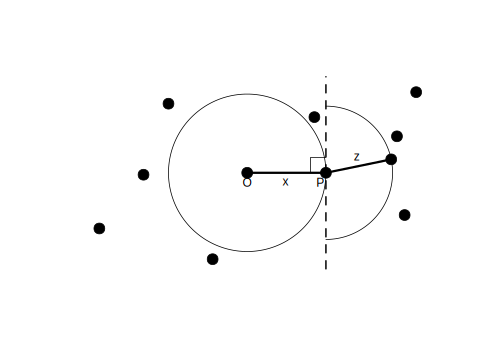
\includegraphics{book_files/figure-latex/unnamed-chunk-233-1} 

}

\caption{Periodic components and their sums.}\label{fig:unnamed-chunk-233}
\end{figure}

다음 예제는 식 \eqref{eq:periodrpg}에서 \(q=3\)일때의 예제다.

\BeginKnitrBlock{example}[주기 시계열]
\protect\hypertarget{exm:unnamed-chunk-234}{}{\label{exm:unnamed-chunk-234} \iffalse (주기 시계열) \fi{} }\(t=1,\ldots,100\)까지 다음의 수열들을 생성해보자.
\[x_{t1}=2\cos (2\pi t 6/100) +3\sin (2\pi t 6 / 100)\]
\[x_{t2}=4\cos (2\pi t 10/100) +5\sin (2\pi t 10 / 100)\]
\[x_{t3}=6\cos (2\pi t 40/100) +7\sin (2\pi t 40 / 100)\]
이들의 시계열들은 위 그림에 나타나있다. \(x_{t1}\)의 진폭은 \(2^{2}+3^{2}=13\)이다. 따라서 \(x_{t1}\)의 최대, 최소값은 \(\pm \sqrt{13}=\pm 3.61\)이다.
마지막으로
\[x_{t}=x_{t1}+x_{t2}+x_{t3}\]
을 고려해본다. 이것의 그림은 위 그림의 오른쪽 아래에 있다. 스펙트럼 분석의 역할은 이렇게 섞여있는 주기 성분들을 분류하고 그들의 상대적 기여도를 계산하는 것이다.

Autocovariance function \eqref{eq:periodrpautocov}를 따라 식 \eqref{eq:periodrpg}에 주어진 모형의 population을 만들어낼 수 있다. 앞으로는 자료 \(x_{1},\ldots , x_{n}\)이 주어졌을 때 실제로 식 \eqref{eq:periodrpvar}를 어떻게 추정할 수 있는가에 대해 살펴볼 것이다.
\EndKnitrBlock{example}

\begin{figure}

{\centering 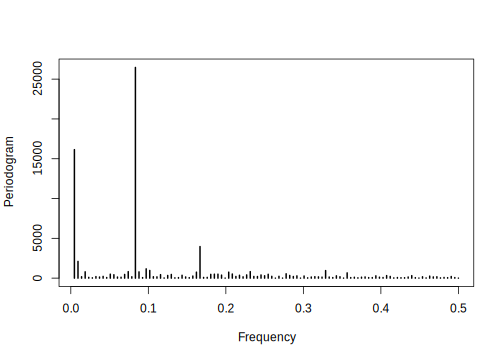
\includegraphics{book_files/figure-latex/unnamed-chunk-235-1} 

}

\caption{Periodogram of the above data.}\label{fig:unnamed-chunk-235}
\end{figure}

앞선 예제의 피리오도그램을 계산해보자. 참고로 scaled periodogram은 다음과 같이 계산된다.

\BeginKnitrBlock{example}[추정과 피리오도그램]
\protect\hypertarget{exm:unnamed-chunk-236}{}{\label{exm:unnamed-chunk-236} \iffalse (추정과 피리오도그램) \fi{} }어떤 시계열의 표본 \(x_{1},\ldots, x_{n}\) (\(n\)은 홀수)이 있다고 하자. 그러면 우리는 다음과 같이 \textbf{정확하게} 쓸 수 있을 것이다.
\EndKnitrBlock{example}

\hypertarget{-spetral-density}{%
\section{스펙트럼 밀도(spetral density)}\label{-spetral-density}}

\textbf{스펙트럼 밀도(spectral density)}는 기초적인 frequency domain tool 중 하나다. 스펙트럼 표현 정리(spectral representation theorem)은 정상시계열을 주기성분들로 분해하는 것에 대한 이론적 근거를 제공한다.

\BeginKnitrBlock{definition}[자기공분산함수의 스펙트럼 표현]
\protect\hypertarget{def:unnamed-chunk-237}{}{\label{def:unnamed-chunk-237} \iffalse (자기공분산함수의 스펙트럼 표현) \fi{} }만약 \(\{x_{t} \}\)가 정상시계열이고 자기공분산 \(\gamma(h)=\text{cov}(x_{t+h},x_{t})\)를 갖는다면 \textbf{스펙트럼 분포(spectral distribution)}이라 불리는 유일한 단조증가 함수가 존재해 \(F(-\infty)=F(-1/2)=0\)이고 \(F(\infty)=F(1/2)=\gamma(0)\)이며

\begin{equation}
\gamma(h)=\int_{-1/2}^{1/2}e^{2\pi i \omega h}dF(\omega)
\label{eq:spectraldistnfct}
\end{equation}

이다.
\EndKnitrBlock{definition}

자기공분산함수가 absolutely summable일 경우 스펙트럼 분포함수는 absolutely continuous하며 \(dF(\omega)=f(\omega)d\omega\)이고 식 \eqref{eq:spectraldistnfct}는 스펙트럼 밀도(spectral density)를 유도한다.

\BeginKnitrBlock{definition}[스펙트럼 밀도]
\protect\hypertarget{def:unnamed-chunk-238}{}{\label{def:unnamed-chunk-238} \iffalse (스펙트럼 밀도) \fi{} }자기공분산함수 \(\gamma(h)\)가 정상과정이며
\begin{equation}
\sum_{h=-\infty}^{\infty}|\gamma(h)|<\infty
\label{eq:abssummablecond}
\end{equation}

를 만족한다고 하면 자기공분산함수는 다음과 같은 표현

\begin{equation}
\gamma(h)=\int_{-1/2}^{1/2}e^{2\pi i \omega h}f(\omega)d\omega, h=0,\pm 1,\pm 2,\ldots
\label{eq:acfrepresentation}
\end{equation}

을 갖고, \textbf{스펙트럼 밀도(spetral density)}는 그것의 역변환

\begin{equation}
f(\omega)=\sum_{h=-\infty}^{\infty}\gamma(h)e^{-2\pi i \omega h}, -1/2 \leq \omega \leq 1/2
\label{eq:spectraldensityrepresentation}
\end{equation}

으로 정의한다.
\EndKnitrBlock{definition}

스펙트럼 밀도는 확률밀도처럼 \(\gamma(h)\)가 non-negative definite이므로
\[f(\omega) \geq 0, \qquad{\forall\omega}\]
을 만족한다. 또한 정의로부터
\[f(\omega)=-f(\omega)\]
이며 이는 스펙트럼 밀도함수가 우함수임을 보여준다. 이런 우함수 성질 덕분에 우리는 보통 \(0<\omega \leq 1/2\)인 \(\omega\)에 대해서만 \(f(\omega)\)를 그리게 된다. 더 나아가 식 \eqref{eq:acfrepresentation}에 \(h=0\)을 넣으면 다음을 얻을 수 있다.
\[\gamma(0)=\text{var}(x_{t})=\int_{-\frac{1}{2}}^{\frac{1}{2}}f(\omega)d\omega.\]
이 말인 즉슨 총분산은 모든 주파수에서의 스펙트럼 분포의 적분 형태로 나타낼 수 있다는 것이다. 이제 자기공분산과 스펙트럼 분포가 같은 정보를 갖고 있다는 것이 분명해졌다. 그러나 그 정보는 다른 형태로 표현된다. 자기공분산 함수는 정보를 lag로 표현하고, 스펙트럼 분포에서는 같은 정보를 cycle을 이용해 표현한다.

또 한가지 중요한 사실은 식 \eqref{eq:acfrepresentation}의 자기공분산 함수 \(\gamma(h)\)와 식 \eqref{eq:spectraldensityrepresentation}의 스펙트럼 밀도는 푸리에 변환의 짝이라는 것이다. 이것은 두 개의 스펙트럼 분포 \(f(\omega),g(\omega)\)가 존재해
\[\gamma_{f}(h)=\int_{-\frac{1}{2}}^{\frac{1}{2}}f(\omega)e^{2\pi i\omega h}d\omega = \int_{-\frac{1}{2}}^{\frac{1}{2}}g(\omega)e^{2\pi i\omega h}d\omega =\gamma_{g}(h), \qquad{\forall 0,\pm1, \pm2,\ldots}\]
을 만족하면
\[f(\omega)=g(\omega)\]
라는 것이다.

마지막으로 식 \eqref{eq:abssummablecond}의 absolutely summable condition 식 \eqref{eq:periodrpautocov}로 만족되어지지 않는다. 그러나 ARMA 모형에 대해서는 만족된다.

\BeginKnitrBlock{example}[백색잡음의 스펙트럼]
\protect\hypertarget{exm:unnamed-chunk-239}{}{\label{exm:unnamed-chunk-239} \iffalse (백색잡음의 스펙트럼) \fi{} }가장 쉬운 예제로 분산이 \(\sigma_{w}^{2}\)인 uncorrelated 확률변수 \(w_{t}\)의 수열의 이론적인 power spectrum을 구해볼 수 있다. 이러한 경우의 자기공분산함수는

\[
\gamma_{w}(h)=
\begin{cases}
\sigma_{w}^{2}, & h\neq 0\\
0, & h=0
\end{cases}
\]

이므로 식 \eqref{eq:spectraldensityrepresentation}로부터
\[f_{w}(\omega)=\sigma_{w}^{2}, \qquad{-0.5\leq \omega \leq 0.5}\]
를 얻을 수 있다. 즉 백색잡음에서는 모든 진동수들의 기여도가 같다.
\EndKnitrBlock{example}

선형과정은 가장 기본적인 과정이므로, 이런 과정의 스펙트럼을 조사하는 것은 의미있는 일이다. 일반적으로, 선형 필터는 투입된 시계열 \(x_{t}\)를 변환하기 위해 특정화된 계수들의 집합 \$a\_\{j\}, j=0, \pm 1, \pm 2, \ldots, \$을 사용하여 다음의 결과물

\begin{equation}
y_{t} =\sum_{j=-\infty}^{\infty}a_{j}x_{t-j}, \qquad{\sum_{j=-\infty}^{\infty}}|a_{j}|<\infty
\label{eq:spectrumconvolution}
\end{equation}

\(y_{t}\)를 만들어 낸다. 식 \eqref{eq:spectrumconvolution}은 통계학에서 \textbf{합성곱(convolution)}이라고 부른다. 계수들 \(a_{j}\)은 \textbf{impulse response function}이라고 부르며, 이것들의 푸리에 변환

\begin{equation}
A(\omega) = \sum_{j=-\infty}^{\infty}a_{j}e^{-2\pi i \omega j}.
\label{eq:IRFFourier}
\end{equation}

을 \textbf{주파수 반응함수(frequency response function)}이라고 부른다. 만약 식 \eqref{eq:spectrumconvolution}에서 \(x_{t}\)가 스펙트럼 밀도 \(f_{x}(\omega)\)를 갖는다고 할 때, 다음의 성질을 얻는다.

\BeginKnitrBlock{proposition}[Output Spectrum of a Filtered Stationary Series]
\protect\hypertarget{prp:unnamed-chunk-240}{}{\label{prp:unnamed-chunk-240} \iffalse (Output Spectrum of a Filtered Stationary Series) \fi{} }만약 식 \eqref{eq:spectrumconvolution}에서 \(x_{t}\)가 스펙트럼 밀도 \(f_{x}(\omega)\)를 갖는다고 할 때 filtered output \(y_{t}\) 의 스펙트럼 \(f_{y}(\omega)\)는 투입값 \(x_{t}\)의 스펙트럼과
\[f_{y}(\omega) = |A(\omega)|^{2}f_{x}(\omega)\]
의 관계를 갖는다.
\EndKnitrBlock{proposition}

앞선 성질을 ARMA 과정에 적용하면 다음을 얻는다.

\BeginKnitrBlock{proposition}[ARMA의 스펙트럼 밀도]
\protect\hypertarget{prp:unnamed-chunk-241}{}{\label{prp:unnamed-chunk-241} \iffalse (ARMA의 스펙트럼 밀도) \fi{} }만약 \(x_{t}\)가 ARMA\((p,q)\)를 따르고 \(\phi(B)x_{t} = \theta(B)w_{t}\)라면, 그것의 스펙트럼 밀도는
\[f_{x}(\omega) = \sigma_{\omega}^{2} \frac{|\theta (e^{-2\pi i \omega})|^{2} }{| \phi(e^{-2\pi i\omega})  |^{2} }\]
이다. 이 떄 \(\phi(z)= 1-\sum_{k=1}^{p} \phi_{k}z^{k}\)이고 \(\theta(z) = 1_ \sum_{k=1}^{q} \theta_{k}z^{k}\)이다.
\EndKnitrBlock{proposition}

스펙트럼을 이용해 확률과정의 총분산(또는 total power)을 각 진동수별로 분해할 수 있다. 스펙트럼은 자기상관함수의 푸리에 변환이므로 자기상관함수와 일대일 관계에 있으며 다음의 성질을 가지고 있다.

\begin{enumerate}
\def\labelenumi{\arabic{enumi}.}
\item
  \(f(\omega)\geq 0\): 음의 값을 갖지 않는 연속 실수함수
\item
  \(f(\omega)=f(\omega + 2\pi)\): 주기가 \(2\pi\)인 주기함수 (\(f(\omega)=f(-\omega)\)인 우함수이므로 일반적으로 \(0\leq \omega \leq \pi\)일 때만 고려한다.)
\item
  \(f(\omega)\)는 확률과정의 \textbf{분산분해(variance decomposition)}으로 해석할 수 있으며, \(f(\omega)d\omega\)는 \((\omega, \omega+d\omega)\)에 속하는 진동수들을 갖는 성분들의 분산에 대한 기여도를 의미한다. 다시 말해 스펙트럼이 어느 영역의 진동수에서 큰 값을 갖는다는 것은 해당 진동수들의 분산에 대한 기여도가 크다는 것을 의미하며, \textbf{이 진동수에 해당되는 주기성분이 시계열의 구성하는 데 가장 중요한 역할을 한다는 것을 의미한다}.
\item
  스펙트럼과 자기공분산함수는 쌍을 이루어 존재하기 때문에 동일한 정보를 제공하는 것이다. 다만 자기공분산함수는 정보를 lag를 이용해 제공하고, 스펙트럼 밀도는 주기를 이용해 정보를 제공한다는 차이점이 있다. 어느 통계량이 더 유용한지는 사용하고자 하는 상황에 따라 다르다고 할 수 있다.
\end{enumerate}

\hypertarget{---periodogram-and-discrete-fourier-transform}{%
\section{피리오도그램과 이산 푸리에 변환(periodogram and discrete Fourier transform)}\label{---periodogram-and-discrete-fourier-transform}}

\BeginKnitrBlock{definition}[이산 푸리에 변환]
\protect\hypertarget{def:unnamed-chunk-242}{}{\label{def:unnamed-chunk-242} \iffalse (이산 푸리에 변환) \fi{} }자료 \(x_{1},\ldots, x_{n}\)이 주어졌을 때, \textbf{이산 푸리에 변환(discrete Fourier transform, DFT)}은
\[d(\omega_{j})=\frac{1}{\sqrt{2}}\sum_{t=1}^{n}x_{t}e^{-2\pi i \omega_{j}t}, j=0,1,\ldots, n-1\]
이며 이 때 \textbf{도수(빈도, frequency)} \(\omega = j/n\)는 \textbf{근본빈도(fundamental frequencies)} 또는 \textbf{푸리에(Fourier)}라고 부른다.
\EndKnitrBlock{definition}

때때로 이산 푸리에 변환의 역버전을 생각하는 것이 편리할 때도 있다.

\BeginKnitrBlock{definition}[이산 푸리에 변환의 역버전]
\protect\hypertarget{def:unnamed-chunk-243}{}{\label{def:unnamed-chunk-243} \iffalse (이산 푸리에 변환의 역버전) \fi{} }\[x_{t}=\frac{1}{\sqrt{2}}\sum_{j=0}^{n-1}d(\omega_{j})e^{2\pi i \omega_{j}t}, t=1,\ldots, n.\]
\EndKnitrBlock{definition}

피리오도그램은 DFT의 squared modulus다.

\BeginKnitrBlock{definition}[피리오도그램]
\protect\hypertarget{def:unnamed-chunk-244}{}{\label{def:unnamed-chunk-244} \iffalse (피리오도그램) \fi{} }\[I(\omega_{j})=|d(\omega_{j})|^{2}, j=0,1,2,\ldots,n-1.\]
\EndKnitrBlock{definition}

\(I(0)=n\bar{x}^{2}\)이다.

\hypertarget{-linear-filters}{%
\section{선형 필터들(linear filters)}\label{-linear-filters}}

\hypertarget{---using-regression-to-discover-a-periodic-signal}{%
\section{주기가 있는 시계열의 회귀분석(using regression to discover a periodic signal)}\label{---using-regression-to-discover-a-periodic-signal}}

다음과 같은 모형
\[x_{t}=A\cos (2\pi\omega t + \phi) + w_{t}\]
을 생각해보자. \(\omega=1/50, A=2,\phi=0.6\pi, \sigma_{w}=5\)일 때 모형은
\[x_{t}=2\cos (2\pi t /50 + 0.6 \pi) + w_{t}\]
가 되며 그림으로 출력하면 다음과 같다.

\begin{figure}

{\centering 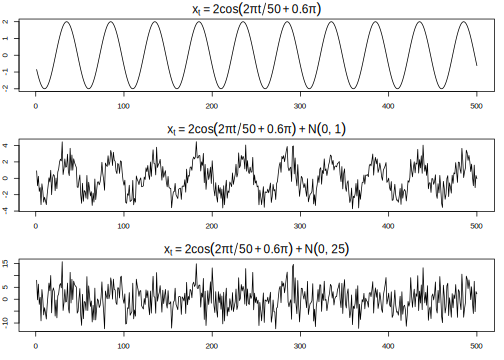
\includegraphics{book_files/figure-latex/unnamed-chunk-245-1} 

}

\caption{Cosine wave with period 50 points (top) with standard Gaussian noise (middle) and with heavy Gaussian noise (bottom).}\label{fig:unnamed-chunk-245}
\end{figure}

진동수 \(\omega=1/50\)이 알려져 있다고 가정하자. 그러나 \(A\)와 \(\phi\)는 모르는 모수라고 가정하자. 삼각함수 공식에 의해
\[A\cos (2\pi \omega t + \phi)=\beta_{1}\cos (2\pi \omega t) + \beta_{2}\sin (2\pi\omega t)\]
이며 \(\beta_{1}=A\cos(\phi), \beta_{2}=-A\sin(\phi)\)이다. 따라서 이 모형은 intercept term을 넣지 않은 일반적인 회귀분석으로 적합할 수 있다.

\hypertarget{-quantile-periodogram}{%
\section{분위수 피리오도그램(quantile periodogram)}\label{-quantile-periodogram}}

분위 회귀분석에 숨어있는 가정은 시계열 \(Y_{t}\)의 \(\alpha\)-분위수가 regressor와 선형 관계를 갖는다는 것이다. 즉 어떤 \(\boldsymbol{\beta}_{0}\neq\mathbf{0}\)에 대해 \(\lambda_{t}=\mathbf{x}_{t}^{T}\boldsymbol{\beta}_{0}\)이 성립한다는 것이다. \textbf{분위수 피리오도그램(quantile periodogram)}에서는 분위수가 숨계진 주기를 포함하고 있는 상황에 관심이 있는 것이다.

\hypertarget{--composite-quantile-periodogram}{%
\section{복합 분위수 피리오도그램(composite quantile periodogram)}\label{--composite-quantile-periodogram}}

\hypertarget{--estimation-of-spectrum}{%
\subsection{스펙트럼의 추정: 피리오도그램(estimation of spectrum)}\label{--estimation-of-spectrum}}

\hypertarget{fourier-analysis}{%
\subsubsection{푸리에분석(Fourier analysis)}\label{fourier-analysis}}

시계열이 관측되었을 때 이들을 진동수에서 정의된 주기성분들로 분해하는 방법을 \textbf{푸리에분석(Fourier analysis)}이라고 한다. 이를 통해 어느 진동수가 중요한 성분이지 따라서 어떤 주기가 시계열에서 중요한 역할을 하는지를 알아낼 수 있다.

\hypertarget{periodogram}{%
\subsubsection{피리오도그램(periodogram)}\label{periodogram}}

스펙트럼을 추정하는 방법을 이해하기 위해서는 \textbf{피리오도그램(periodogram)}에 대한 이해가 필요하다. 이 절의 서술은 \citep{Lim2013}을 참고하였다. 또 다른 참고자료로는 \citep{Shumway2010}이 있다.

다음과 같은 시계열 자료의 수열 \(\{Y_{1}, \ldots, Y_{n}\}\)을 관측한다고 하자. 그러면 \textbf{피리오도그램(periodogram)} \(I_{n}(\omega)\)는
\[I_{n}(\omega)=\frac{1}{n}| \sum_{i=1}^{n}Y_{i}e^{-it\omega}|^{2}\]
로 정의된다. 이 때 \(\omega\in (0,\pi)\)는 \textbf{진동수모수(frequency parameter)}이다. \(\omega\)가 푸리에 진동수(\(\omega=\frac{2\pi k}{n}, k\in\mathbb{Z}\))일 때 이 피리오도그램은
\[I_{n}(\omega)=\frac{n}{4}\| \tilde{\boldsymbol{\beta}}_{n}(\omega)\|^{2}\]
으로 표현할 수 있다고 한다\citep{Li2008}. 여기서 \(\| \cdot \|\)은 벡터의 \(l_{2}\) 노름이며 \(\tilde{\boldsymbol{\beta}}_{n}(\omega)\)은 최소자승법
\[\tilde{\boldsymbol{\beta}}_{n}(\omega)=\text{arg}\min_{\boldsymbol{\beta}\in\mathbb{R}^{2}}\sum_{i=1}^{n}| Y_{i}-\mathbf{x}_{t}^{T}(\omega)\boldsymbol{\beta}|^{2}\]
의 해다. 그리고 이 때 \(\mathbf{x}_{t}(\omega)=(\cos(\omega t), \sin (\omega t))^{T}\)로 harmonic regressor다.

\hypertarget{r-r-periodogram}{%
\section{R 예제(R-periodogram)}\label{r-r-periodogram}}

여기서는 R에서 피리오도그램을 그리는 방법에 대해 다뤄보겠다.

\begin{enumerate}
\def\labelenumi{\arabic{enumi}.}
\tightlist
\item
  직접 구현
\end{enumerate}

다음 예제는 \citep{Shumway2010}에 있는 scaled periodogram을 구하는 예제이다.

\begin{enumerate}
\def\labelenumi{\arabic{enumi}.}
\setcounter{enumi}{1}
\tightlist
\item
  이미 구현된 패키지 안의 함수들을 이용하는 경우
\end{enumerate}

여기서는 서울특별시 PM10의 1998년 1월부터 2014년 12월까지의 월별 시계열 자료를 이용해 피리오도그램을 그려보겠다.

\begin{Shaded}
\begin{Highlighting}[]
\NormalTok{dataspec <-}\StringTok{ }\KeywordTok{read.csv}\NormalTok{(}\StringTok{'~/Dropbox/Data/PM/MonthlyPMSeoul.csv'}\NormalTok{, }\DataTypeTok{header=}\NormalTok{T)}
\NormalTok{dataspec <-}\StringTok{ }\NormalTok{dataspec[,}\OperatorTok{-}\DecValTok{1}\NormalTok{]}
\NormalTok{dataspec <-}\StringTok{ }\KeywordTok{t}\NormalTok{(dataspec)}
\NormalTok{time_index_month <-}\StringTok{ }\KeywordTok{seq}\NormalTok{(}\DataTypeTok{from =} \KeywordTok{as.POSIXct}\NormalTok{(}\StringTok{"1998-01-01"}\NormalTok{), }\DataTypeTok{to =} \KeywordTok{as.POSIXct}\NormalTok{(}\StringTok{"2014-12-01"}\NormalTok{), }\DataTypeTok{by =} \StringTok{"month"}\NormalTok{)}
\NormalTok{dataspec <-}\StringTok{ }\KeywordTok{xts}\NormalTok{(dataspec[,}\DecValTok{1}\NormalTok{], }\DataTypeTok{order.by=}\NormalTok{time_index_month)}
\KeywordTok{plot}\NormalTok{(dataspec, }\DataTypeTok{type=}\StringTok{'o'}\NormalTok{, }\DataTypeTok{ylim=}\KeywordTok{c}\NormalTok{(}\DecValTok{0}\NormalTok{,}\DecValTok{150}\NormalTok{), }\DataTypeTok{xlab=}\StringTok{"Month"}\NormalTok{, }\DataTypeTok{main=}\StringTok{"Monthly"}\NormalTok{)}
\end{Highlighting}
\end{Shaded}

\begin{figure}

{\centering 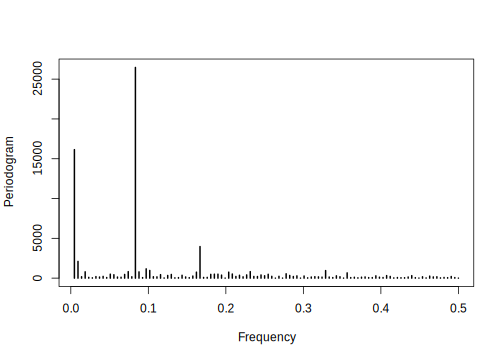
\includegraphics{book_files/figure-latex/unnamed-chunk-246-1} 

}

\caption{Time series of Seoul PM10.}\label{fig:unnamed-chunk-246}
\end{figure}

\texttt{TSA}, \texttt{kza}, \texttt{itsmr} 패키지를 이용한다. 같은 이름의 함수를 사용하기 때문에 실행할 때 주의해야 한다.

\begin{Shaded}
\begin{Highlighting}[]
\NormalTok{TSA}\OperatorTok{::}\KeywordTok{periodogram}\NormalTok{(dataspec, }\DataTypeTok{log=}\StringTok{'yes'}\NormalTok{)}
\end{Highlighting}
\end{Shaded}

\begin{figure}

{\centering 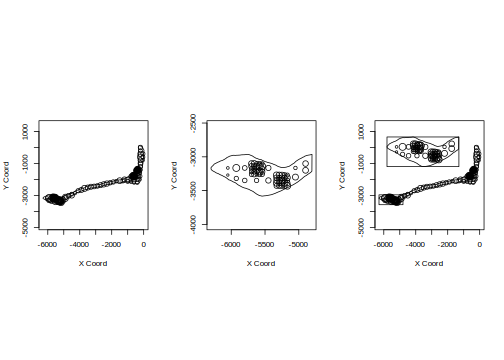
\includegraphics{book_files/figure-latex/unnamed-chunk-247-1} 

}

\caption{Periodogram (using R package TSA).}\label{fig:unnamed-chunk-247}
\end{figure}

\begin{Shaded}
\begin{Highlighting}[]
\KeywordTok{plot}\NormalTok{(kza}\OperatorTok{::}\KeywordTok{periodogram}\NormalTok{(}\KeywordTok{as.numeric}\NormalTok{(dataspec)), }\DataTypeTok{type=}\StringTok{'o'}\NormalTok{)}
\end{Highlighting}
\end{Shaded}

\begin{figure}

{\centering 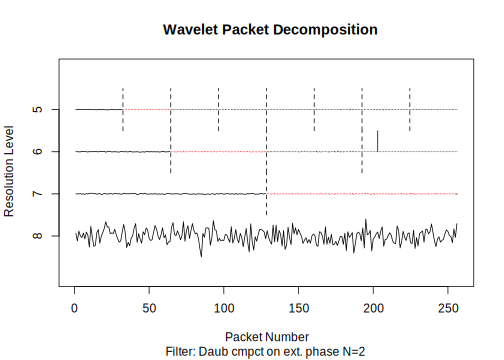
\includegraphics{book_files/figure-latex/unnamed-chunk-248-1} 

}

\caption{Periodogram (using R package kza).}\label{fig:unnamed-chunk-248}
\end{figure}

\begin{Shaded}
\begin{Highlighting}[]
\KeywordTok{plot}\NormalTok{(itsmr}\OperatorTok{::}\KeywordTok{periodogram}\NormalTok{(dataspec))}
\end{Highlighting}
\end{Shaded}

\begin{figure}

{\centering 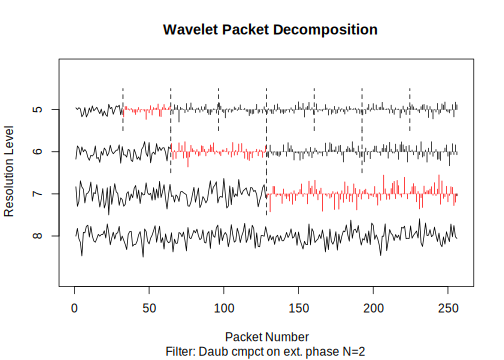
\includegraphics{book_files/figure-latex/unnamed-chunk-249-1} 

}

\caption{Periodogram (using R package itsmr).}\label{fig:unnamed-chunk-2491}
\end{figure}
\begin{figure}

{\centering 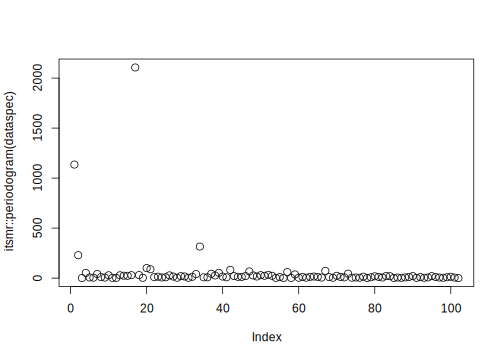
\includegraphics{book_files/figure-latex/unnamed-chunk-249-2} 

}

\caption{Periodogram (using R package itsmr).}\label{fig:unnamed-chunk-2492}
\end{figure}

\hypertarget{part-multiscale-methods-in-statistics}{%
\part{Multiscale Methods in Statistics}\label{part-multiscale-methods-in-statistics}}

\hypertarget{fouriertowavelet}{%
\chapter{푸리에로부터 웨이블릿으로}\label{fouriertowavelet}}

이 절의 초반부 내용은 \citep{Ogden2012}를 참고하였다.

\hypertarget{-discrete-fourier-transform}{%
\section{이산 푸리에변환(discrete Fourier transform)}\label{-discrete-fourier-transform}}

\BeginKnitrBlock{definition}[L2]
\protect\hypertarget{def:unnamed-chunk-250}{}{\label{def:unnamed-chunk-250} \iffalse (L2) \fi{} }어떤 함수 \(f\)가 \(L^{2}[a,b]\)에 속한다는 것은
\[\int_{a}^{b}f^{2}(x)dx <\infty\]
를 만족할 때이다.
\EndKnitrBlock{definition}

푸리에 급수는 푸리에 변환의 inversion formula이다. \citep{Jiang2010} 푸리에 변환은 \(f\in L^{2}[-\pi, \pi]\)인 어떤 함수 \(f\)는 다음과 같이 지수함수로 표현할 수 있다는 것이다.
\[\hat{f}(k)=\frac{1}{2\pi}\int_{-\pi}^{\pi}f(x)e^{-ikx}dx,\]
이 때 \(k=0,\pm 1, \pm 2\) 등이고 \(i=\sqrt{-1}\)이다. \(f\)는 적분가능한 함수이다. 푸리에 변환이 주어지면 푸리에 급수로 \(f\)를 복원할 수 있다.
\[f(x)=\sum_{k=-\infty}^{\infty}\hat{f}(k)e^{ikx}=\sum_{k=-N}^{N}\hat{f}(k)e^{ikx}+o(1),\]
이때 \(N\)은 양의 정수이고 remaining term은 \(N\rightarrow\infty\)일 때 \(o(1)\)이다.

같은 방법으로 사인함수와 코사인함수의 무합급수로 표현할 수 있다는 것이다.
\[f(x)=\frac{1}{2}a_{0}+\sum_{j=1}^{\infty}(a_{j}\cos (jx) + b_{j}\sin (jx)),\]
여기서 \(\{ a_{0}, a_{1}, b_{1}, \ldots \}\)들은 계수다.

\BeginKnitrBlock{definition}[직교]
\protect\hypertarget{def:unnamed-chunk-251}{}{\label{def:unnamed-chunk-251} \iffalse (직교) \fi{} }두 함수 \(f_{1},f_{2}\in L^{2}[a,b]\)는 \(<f_{1},f_{2}=0\)일 때 \textbf{직교(orthogonal)}라고 부른다.
\EndKnitrBlock{definition}

\BeginKnitrBlock{definition}[직교정규]
\protect\hypertarget{def:unnamed-chunk-252}{}{\label{def:unnamed-chunk-252} \iffalse (직교정규) \fi{} }함수들의 수열 \(\{ f_{j} \}\)는 모든 \(f_{j}\)들이 짝지은 직교(pairwise orthogonal)이며 \(\| f_{j}\|=1\)일 때 \textbf{직교정규(orthonormal)}이라고 한다.
\EndKnitrBlock{definition}

\hypertarget{time-frequency-analysis}{%
\section{시간주파수해석(time-frequency analysis)}\label{time-frequency-analysis}}

신호를 시간의 관점에서 해석하는 것을 \textbf{시간해석(time analysis)}라고 한다. 반면에 푸리에해석은 주파수의 관점에서 해석하는 \textbf{주파수해석(frequency analysis)}이다. 우리가 일상생활에서 접하는 신호들은 시간과 주파수를 동시에 고려해야 하는 것들이 많다. 예를 들어, 악보의 각 음표는 어느 시점에 그 음을 발성할 것인지를 나타내는 동시에 어떤 음높이로 발성할 것인지를 나타낸다. 즉 발성할 시점은 시간해석의 관점에서 보는 것이고, 음높이는 주파수해석의 관점에서 보는 것이다. 따라서, 노래라는 신호를 시간해석 또는 주파수해석 각각으로 해석해서는 결코 만족스러운 결과를 얻을 수 없을 것이다. 오늘날 가장 널리 연구되고 사용되는 시간주파수해석법은 웨이블릿의 사용하는 것이다.

\hypertarget{wavelet}{%
\section{웨이블릿(wavelet)}\label{wavelet}}

웨이블릿은 뒷장에서도 다시 설명하겠지만, 여기서는 \citep{Shima2016}의 내용을 다룬다.

앞서 보았듯이, 푸리에 변환은 시간 영역에서 진동이 있는 요소들을 추출해낸다는 점에서 효율적인 툴로 알려져있다. 그러나 푸리에 변환은 시간 영역과 주파수 영역을 동시에 보지 못한다는 한계가 있고, 이를 극복하고자 웨이블릿이 등장했다. 웨이블릿 분석의 큰 장점은 신호에 있는 복잡한 정보들을 \textbf{웨이블릿(wavelet)}이라고 하는 기본적인 함수들로 분해(decomposition)할 수 있다는 것이다. 웨이블릿은 localized waveform으로 시간 및 주파수 스케일의 다양한 범위를 컨트롤할 수 있게 해준다. 또 이 성질은 복구(reconstruction)를 가능하게 해 준다.

푸리에 해석에서의 주파수와는 달리, 웨이블릿 해석에서는 \textbf{척도(scale)}가 중요한 역할을 한다. 척도가 큰 창(window)을 통해서 신호를 관찰하면, 그 신호의 전반적인 특징을 관찰할 수 있다. 즉 웨이블릿이라는 창을 사용해서 신호를 분석하면 신호의 전체적인 모습뿐 아니라 세부적인 모습까지도 분석할 수 있다. 따라서 신호가 가지고 있는 비정상적(nonstationry) 성질들을 나타내는 데 웨이블릿이 유용하다. 예를 들어, 푸리에 해석에서는 신호의 불연속성, 단절(rupture) 등을 잘 식별할 수 없지만 웨이블릿 해석을 사용하면 식별이 가능하다. 이는 웨이블릿이 단순히 신호의 자세한 부분까지를 반영하기 때문이 아니라 신호가 변화하는 부분을 잘 나타내기 때문이다.

\BeginKnitrBlock{definition}[웨이블릿]
\protect\hypertarget{def:unnamed-chunk-253}{}{\label{def:unnamed-chunk-253} \iffalse (웨이블릿) \fi{} }\textbf{웨이블릿(wavelet)} \(\psi(t)\)는 실변수함수로, localized waveform을 갖으며

\begin{enumerate}
\def\labelenumi{\arabic{enumi}.}
\item
  \(\int_{-\infty}^{\infty}\psi(t)dt=0\)
\item
  \(\int_{-\infty}^{\infty}\psi(t)^{2}dt=1\)
\item
  \(\psi(t)\)의 푸리에 변환 결과인 \(\Psi(t)\)가 \textbf{admissibility condition}이라 불리는 다음 성질
  \[C_{\Psi}\equiv\int_{0}^{\infty}\frac{|\Psi(\omega) |^{2}}{\omega}d\omega <\infty\]
  를 만족한다. 이 때 \(C_{\Psi}\)를 \textbf{admissibility constant}라고 부르며 이 값은 \(\psi(t)\)의 explicit t-dependence에 의존한다고 한다.
\end{enumerate}
\EndKnitrBlock{definition}

\BeginKnitrBlock{example}[Haar 웨이블릿]
\protect\hypertarget{exm:unnamed-chunk-254}{}{\label{exm:unnamed-chunk-254} \iffalse (Haar 웨이블릿) \fi{} }\textbf{Haar 웨이블릿(Haar wavelet)}은

\begin{equation} 
\psi(t) \equiv
  \begin{cases}
    \frac{1}{\sqrt{2}}       & \quad t\in (0,1],\\
    \frac{-1}{\sqrt{2}}  & \quad t\in (-1,0],\\
    0   & \quad \text{otherwise} \\
  \end{cases}
\end{equation}

으로 정의된다.
\EndKnitrBlock{example}

\begin{figure}

{\centering 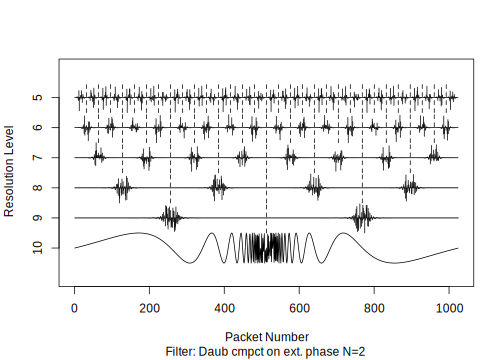
\includegraphics{book_files/figure-latex/unnamed-chunk-255-1} 

}

\caption{Haar wavelet function.}\label{fig:unnamed-chunk-255}
\end{figure}

한 마디로 정리하자면 웨이블릿은 localized oscillating wave라고 볼 수 있다.

\hypertarget{-wavelet-transform}{%
\section{웨이블릿 변환(wavelet transform)}\label{-wavelet-transform}}

수학적 용어로 \textbf{웨이블릿 변환}은 웨이블릿의 \textbf{합성곱(convolution)}이다. 여기서 잠시 합성곱에 대해 살펴보면, \(f\), \(g\)라는 두 함수의 \([0,t]\)까지 범위에서 합성곱은
\[\int_{0}^{\tau}f(\tau)g(t-\tau)d\tau\]
이다.

이 합성곲은 웨이블릿의 모양을 변화시키기 위해 두 모수를 갖는다. 하나는 \(a\)로 표시되는 \textbf{팽창모수(dilatation parameter)}이며, domain에서 웨이블릿의 팽창과 수축을 결정해준다. 다른 하나는 \(b\)로 표시되는 \textbf{이동모수(translation parameter)}로, 축을 따라 웨이블릿을 움직여준다.

\begin{figure}

{\centering \includegraphics[width=17.5in]{images/multiscale_Transform} 

}

\caption{(a) Dilatation and (b) translation of a wavelet.}\label{fig:unnamed-chunk-256}
\end{figure}

일례로 이동하고 전이된 버전의 Mexican hat wavelet은
\[\psi(\frac{t-b}{a})=[1-(\frac{t-b}{a})^{2}]e^{[-\frac{1}{2}\cdot (\frac{t-b}{a})^{2}]}\]
이 된다. (\(\sigma=1\)인 경우)

\BeginKnitrBlock{definition}[웨이블릿 변환]
\protect\hypertarget{def:unnamed-chunk-257}{}{\label{def:unnamed-chunk-257} \iffalse (웨이블릿 변환) \fi{} }연속신호 \(x(t)\)의 웨이블릿 \(\psi(t)\)에 대한 \textbf{웨이블릿 변환(wavelet transform)} \(T(a,b)\)는
\[T(a,b)=w(a)\int_{-\infty}^{\infty}x(t)\psi(\frac{t-b}{a})dt\]
로 정의된다. 여기서 \(w(a)\)는 \textbf{가중치함수(weighted function)}이라고 부른다.

여기서 좀 더 컴팩트한 표현으로
\[\psi_{a,b}(t)=\frac{1}{\sqrt{a}}\psi(\frac{t-b}{a})\]
를 정의해 앞선 식을
\[T(a,b)=\int_{-\infty}^{\infty}x(t)\psi_{a,b}(t)dt\]
로 쓸 수 있다. 앞으로 \(\psi_{a,b}(t)\)을 단순히 \textbf{웨이블릿}으로 부르기로 한다.
\EndKnitrBlock{definition}

일반적으로 \(w(a)=\frac{1}{\sqrt{a}}\)로 정의하는데 그 이유는
\[\int_{-\infty}^{\infty}[\frac{1}{\sqrt(a)}\psi(\frac{t-b}{a})]^{2}dt=\int_{-\infty}^{\infty}\psi(u)^{2}du = 1 \qquad{ \text{ with } u=\frac{t-b}{a}}\]
이기 때문이다.

정리하면 웨이블릿 변환은 time-varying signal에 대한 현미경 역할을 한다.

\hypertarget{-wavelet-space}{%
\section{웨이블릿 공간(wavelet space)}\label{-wavelet-space}}

\hypertarget{-multiresolution-analysis}{%
\subsection{다중해상도 분석(multiresolution analysis)}\label{-multiresolution-analysis}}

다중해상도 분석은 사실 함수공간의 집합(a set of function space)이다. 혼란스럽게 용어가 정의되어 있어 주의를 필요로 한다.

\BeginKnitrBlock{definition}[다중해상도 분석]
\protect\hypertarget{def:unnamed-chunk-258}{}{\label{def:unnamed-chunk-258} \iffalse (다중해상도 분석) \fi{} }\textbf{다중해상도 분석(multiresolution analysis)}란 \(L^{2}(\mathbb{R})\)의 닫힌 부분공간(closed subspace)의 함수공간의 집합 \(\mathcal{V}_{j}:j\in\mathbb{Z}\)으로 \(\mathcal{V}_{j}\)는 다음 조건을 만족한다.

\begin{enumerate}
\def\labelenumi{\arabic{enumi}.}
\item
  \(\cdots \subset \mathcal{V}_{-2} \subset \mathcal{V}_{-1} \subset \mathcal{V}_{0} \subset \mathcal{V}_{1} \subset \mathcal{V}_{2} \ldots \subset L^{2}(\mathbb{R})\)
\item
  \(\bigcap_{j=-\infty}^{\infty}\mathcal{V}_{j}=\{0\}\)
\item
  \(f(t)\in\mathcal{V}_{j}\) if and only if \(f(2t)\in\mathcal{V}_{j+1}\) for all integer \(j\)
\item
  집합 \(\{ \phi (t-n), n \in \mathbb{Z}\}\)가 \(\mathcal{V}_{0}\)의 직교정규기저(orthonormal basis)가 되도록 하는 함수 \(\phi(t)\in\mathcal{V}_{0}\)이 존재한다.
\end{enumerate}
\EndKnitrBlock{definition}

이 때 \(\phi(t)\)를 \textbf{척도함수(scaling function)} 또는 \textbf{부웨이블릿(father wavelet)}이라고 부른다. 참고할만한 사항으로 다중해상도 분석의 정의는 \(\phi(t)\)의 존재에 대한 어떤 정보도 주지 않는다. 그러나 우리가 만약 바람직한 함수 \(\phi(t)\)를 찾는다면 \(\{ \phi(t-n), n\in\mathbb{Z}\}\)가 span하는 함수공간 \(\mathcal{V}_{0}\)를 정의할 수 있고 앞선 정의의 3번을 이용해 \(V_{j}\)들을 계속해서 만들어내 다중해상도 분석 \(\mathcal{V}_{j}\)를 만들 수 있다. 즉 다시말하면 척도함수 \(\phi(t)\)가 다중해상도 분석 \(\{ \mathcal{V}_{j}\}\)를 생성한다.

\BeginKnitrBlock{definition}[다중해상도 분석의 예]
\protect\hypertarget{def:unnamed-chunk-259}{}{\label{def:unnamed-chunk-259} \iffalse (다중해상도 분석의 예) \fi{} }\(L^{2}(\mathbb{R})\)에서 어떤 구간 \([2^{-m}n, 2^{-m}(n+1)], \forall n\in\mathbb{Z}\)에서만 상수값을 갖는 모든 함수들의 집합 \(\mathcal{V}_{m}\)을 생각해보자. 그러면 \(\mathcal{V}_{m}\)은 다중해상도 분석의 조건 1부터 3까지를 만족시킨다(\(\phi\)들은 기저이다. 잘 생각해 볼 것)
\EndKnitrBlock{definition}

\begin{figure}

{\centering \includegraphics[width=17.44in]{images/multiscale_Multiscaleanalysis} 

}

\caption{(a) Dilatation and (b) translation of a wavelet.}\label{fig:unnamed-chunk-260}
\end{figure}

위 그림에 나오는 \(\{\phi(t-n),n\in\mathbb{Z}\}\)는

\begin{equation} 
\phi(t) \equiv
  \begin{cases}
    1    & \quad 0 \leq t \leq 1\\
    0    & \quad \text{otherwise} \\
  \end{cases}
\end{equation}

로 정의되며 다중해상도분석의 4번 조건을 만족한다. 즉, 어떤 함수 \(f\in\mathcal{V}_{0}\)은
\[f(t)=\sum_{n=-\infty}^{\infty}c_{n}\phi(t-n)\]
으로 표현가능하다. 여기서 \(c_{n}\)은 적절한 상수이다. 따라서 공간 \(\mathcal{V}_{m}\)은 \(\phi(t)\)로 생성되어지는 다중해상도 분석이다.

\hypertarget{orthogonal-decomposition}{%
\subsection{직교분해(orthogonal decomposition)}\label{orthogonal-decomposition}}

다중해상도 분석이 중요한 것은 이것이 \(L^{2}(\mathbb{R})\)에서의 직교정규 기저(orthonormal basis, i.e.~a complete orthonormal set of functions)를 구성할 수 있게 해준다는 것이다. 이 말을 입증하기 위해 우선 다중해상도 분석 \(\{\mathcal{V}_{j}\}\)가 다음 관계
\[\mathcal{V}_{0}\subset\mathcal{V}_{1}\subset\mathcal{V}_{2}\subset\cdots \subset L^{2}\]
를 만족한다는 것이다.

이제 다음과 같이 \(\mathcal{V}_{0}\)와 \(\mathcal{V}_{1}\)의 \textbf{직교 여공간(orthogonal complement)} \(\mathcal{W}_{0}\)
\[\mathcal{V}_{1}=\mathcal{V}_{0}\oplus\mathcal{W}_{0}\]
을 정의한다. 여기서 \(\oplus\)는 주어진 벡터공간들의 \textbf{직합(direct sum)}이다. 공간 \(\mathcal{W}_{0}\)을 0차원에서의 \textbf{웨이블릿 공간(wavelet space)}이라고 부른다.

\begin{figure}

{\centering \includegraphics[width=12.17in]{images/multiscale_Orthogonalcomplement} 

}

\caption{Hierarchical structure of the space V and W as subspace of L2.}\label{fig:unnamed-chunk-261}
\end{figure}

위 식은
\[\mathcal{V}_{2}=\mathcal{V}_{1}\oplus\mathcal{W}_{1}=\mathcal{V}_{0}\oplus\mathcal{W}_{0}\oplus\mathcal{W}_{1}\]
으로 확장할 수 있으며, 일반적으로 확장하면
\[L^{2}=\mathcal{V}_{\infty}=\mathcal{V}_{0}\oplus \mathcal{W}_{0} \oplus \mathcal{W}_{1} \oplus \mathcal{W}_{2} \oplus \cdots\]
로 쓸 수 있다. 여기서 \(\mathcal{V}_{0}\)은 함수들의 집합 \(\{ \phi(t-n), n\in\mathbb{Z}\}\)으로 span하는 initial space이다.

최초 공간을 임의로 설정할 수 있기 때문에, 다음과 같이
\[L^{2}=\mathcal{V}_{5}\oplus \mathcal{W}_{5} \oplus \mathcal{W}_{6}\cdots\]
으로 높게 고르거나 또는
\[L^{2}=\mathcal{V}_{-3}\oplus \mathcal{W}_{-3} \oplus \mathcal{W}_{-2}\cdots\]
와 같이 낮은 해상도를 고를 수도 있다. 극단적으로는
\[L^{2}=\cdots\oplus \mathcal{W}_{-1} \oplus \mathcal{W}_{0} \oplus \mathcal{W}_{1}\cdots\]
로 \(-\infty\)를 취하기도 한다. 이와 같은 표현을 \(L^{2}\)에서의 \textbf{직교분해(orthogonal decomposition)}으로 부른다. 이것은 즉 어떤 함수 \(x\in L^{2}(\mathbb{R})\)은 다음과 같이
\[x(t)=\cdots + g_{-1}(t)+g_{0}(t)+g_{1}(t)+\cdots .\]
\(g_{j}\in\mathcal{W}_{j}\)의 무한합으로 분해할 수 있다.

\begin{figure}

{\centering \includegraphics[width=6.11in]{images/multiscale_spacedecomp} 

}

\caption{Hierarchical structure of the space V and W.}\label{fig:unnamed-chunk-262}
\end{figure}

\hypertarget{--orthonormal-basis-construction}{%
\subsection{직교정규 기저 구성(orthonormal basis construction)}\label{--orthonormal-basis-construction}}

웨이블릿 공간 \(\{ W_{j} \}\)들의 직교 성질에 대해 좀 더 자세히 살펴보자. 앞선 직합으로 표시된 식들에 의해
\[\mathcal{W}_{0}\subset \mathcal{V}_{1} \text{ and } \mathcal{W}_{1} \subset \mathcal{V}_{2}\]
관계를 갖는다. 다중해상도 분석 \(\{\mathcal{V}_{j}\}\)의 정의의 관점에서 봤을 때,
\[f(t)\in \mathcal{V}_{1} \Longleftrightarrow f(2t)\in \mathcal{V}_{2}\]
이고 그러므로
\[f(t)\in \mathcal{W}_{0} \Longleftrightarrow f(2t)\in \mathcal{W}_{1}\]
이다. 더 나아가서, 다중해상도 분석의 4번 조건은
\[f(t)\in \mathcal{W}_{0} \Longleftrightarrow f(t-n)\in\mathcal{W}_{0} \text{ for any } n\in\mathbb{Z}\]
가 되게 만든다.

이제 위 사실들을 가지고 \(L^{2}(\mathbb{R})\)에서의 직교정규 기저들을 만들어보자. 우선 \(\mathcal{W}_{0}\)에서 직교정규 기저 \(\{\psi(t-n),n\in\mathbb{Z}\}\)를 만드는 함수\(\psi(t)\)가 있다고 하자. 그러면 다음과 같은 표기
\[\phi_{0,n}(t)\equiv\psi(t-n)\in\mathcal{W}_{0]}\]
를 이용해 이것의 scaled version을
\[\phi_{1,n}(t)=\sqrt{2}\psi(2t-n)\]
으로 정의하고 이것은 \(\mathcal{W}_{1}\)의 직교정규 기저가 된다. \(\sqrt{2}\)는 정규 조건을 유지하기 위해 들어간 상수다.
\[\int_{-\infty}^{\infty}\psi_{0,n}(t)^{2}dt=\int_{-\infty}^{\infty}\psi_{1,n}(t)^{2}dt=1.\]

같은 과정들을 반복하면
\[\psi_{m,n}(t)=2^{m/2}\psi(2^{m}t-n)\]
이라는 관계식을 얻을 수 있으며 이 때 \(\psi_{m,n}\)은 \(\mathcal{W}_{m}\)의 직교기저가 된다. 이러한 결과물들을 앞선 함수 \(x\in L^{2}(\mathbb{R})\)의 직교분해 식에 넣을 경우

\begin{eqnarray*}
x(t)&=& \cdots + g_{-1}(t)+g_{0}(t)+g_{1}(t)+\cdots\\
&=&\cdots + \sum_{n=-\infty}^{\infty}c_{-1,n}\psi_{-1,n}(t)+\sum_{n=-\infty}^{\infty}c_{0,n}\psi_{0,n}(t) + \sum_{n=-\infty}^{\infty}c_{1,n}\psi_{1,n}(t)+\cdots \\
&=&\sum_{m=-\infty}^{\infty}\sum_{n=-\infty}^{\infty}c_{m,n}\psi_{m,n}(t).
\end{eqnarray*}

결과적으로 family \(\psi_{m,n}(t)\)가 \(L^{2}(\mathbb{R})\)의 직교정규 기저가 된다. 위 결과를 다음 정리로 요약할 수 있다.

\BeginKnitrBlock{theorem}[직교정규 기저의 구성]
\protect\hypertarget{thm:unnamed-chunk-263}{}{\label{thm:unnamed-chunk-263} \iffalse (직교정규 기저의 구성) \fi{} }\(\{ \mathcal{V}_{j}\}\)를 다중해상도 분석이라고 하고 공간 \(\mathcal{W}_{0}\)를 \(\mathcal{W}_{0}=\mathcal{V}_{1}/\mathcal{V}_{0}\)으로 정의한다. 만약 어떤 함수 \(\psi(t)\)가 \(\mathcal{W}_{0}\)의 정규직교 기저 \(\{ \psi(t-n),n\in\mathbb{Z}\}\)를 만들어 낸다면, 함수들의 집합 \(\{\psi_{m,n},m,n\in\mathbb{Z}\}\)는
\[\psi_{m,n}(t)=2^{m/2}\psi(2^{m}t-n)\]
\(L^2{\mathbb{R}}\)에서의 직교정규 기저를 구성한다.
\EndKnitrBlock{theorem}

여기서 소개된 \(\psi(t)\)는 웨이블릿을 결정하는 데, 즉 Haar wavelet이냐 mexican hat wavelet이냐 등을 결정하는 데 쓰이므로, \(\mathcal{W}_{m}\)을 \textbf{웨이블릿 공간(wavelet space)}이라고 부르며 함수 \(\psi(t)\)를 \textbf{모웨이블릿(mother wavelet)}이라고 부른다.

\hypertarget{--two-scale-relation}{%
\subsection{두-스케일 관계(two-scale relation)}\label{--two-scale-relation}}

앞서 언급한 내용들은 \(L^{2}(\mathbb{R})\)에서의 직교정규 기저 \(\{\psi_{m,n} \}\)을 모웨이블릿 \(\psi(t)\)의 명시적 함수 형태를 특정지음으로써 구성할 수 있다는 것을 암시한다. 그럼 이제 남아있는 일은 모웨이블릿 \(\psi(t)\)를 이용해 다중해상도 분석이 주어졌을 때 \(\mathcal{W}_{0}=\mathcal{V}_{1}/\mathcal{V}_{0}\)이 포함된 공간에서 정규직교 기저 \(\{ \psi(t-n), n\in\mathbb{Z}\}\)를 이끌어내는 일이다. 우리는 \(\psi(t)\)를 척도함수 \(\phi(t)\)를 잘 살펴봄으로써 찾아낼 수 있었음을 상기해야 한다.

다음에는 주어진 다중해상도 분석에서 모웨이블릿 \(\psi(t)\)를 구성하기 위한 척도함수의 중요한 특징인 \textbf{두-스케일 관계(two-scale relation)}에 대해 언급하겠다. 우리는 \(\mathcal{V}_{m}\)에 있는 모든 함수들이 \(\mathcal{V}_{0}\)에 있는 것들에서 \(2^{m}\)만큼 스케일링하여 얻을 수 있다는 걸 안다. 이 결과를 스케일링 함수에 적용시키면
\[\phi_{0,n}(t)\equiv \phi(t-n) \in \mathcal{V}_{0}\]
이고 이것은
\[\phi_{m,n}(t)=2^{m/2}\phi(2^{m}t-n), m\in\mathbb{Z}\]
가 \(\mathcal{V}_{m}\)의 직교정규 기저가 되는 것으로 이어진다. 특히 \(\phi \in \mathcal{V}_{0}\subset \mathcal{V}_{1}\)이고 \(\phi_{1,n}(t)=\sqrt{2}\phi(2t-n)\)이 \(\mathcal{V}_{1}\)의 직교정규 기저이기 때문에, \(\phi(t)\)는 \(\phi_{1,n}(t)\)에 의해 확장되어질 수 있다. 이것은 다음 정리로 요약할 수 있다.

\BeginKnitrBlock{theorem}[두-스케일 관계]
\protect\hypertarget{thm:unnamed-chunk-264}{}{\label{thm:unnamed-chunk-264} \iffalse (두-스케일 관계) \fi{} }척도함수 \(\phi(t)\)가 다중척도 해석 \(\{ \mathcal{V}_{j}\}\)을 생성할 때, 다음과 같은 관계식을 얻을 수 있다.
\[\phi(t)=\sum-{n=-\infty}^{\infty}p_{n}\phi_{1,n}(t)=\sqrt{2}\sum_{n=-\infty}^{\infty}p_{n}\phi(2t-n),\]
이 때
\[p_{n}=\int_{-\infty}^{\infty}\phi(t)\phi_{1,n}(t)dt\]
이다. 이 식을 \(\phi(t)\)의 \textbf{두-스케일 관계(two-scale relation)}식이라고 부른다. 그리고 계수 \(p_{n}\)을 \textbf{척도함수계수(scaling function coefficients)}라고 부른다.
\EndKnitrBlock{theorem}

\BeginKnitrBlock{example}[두-스케일 관계의 예]
\protect\hypertarget{exm:unnamed-chunk-265}{}{\label{exm:unnamed-chunk-265} \iffalse (두-스케일 관계의 예) \fi{} }다음과 같이 \(L^{2}(\mathbb{R})\)의 함수들을 모두 포함하고 구간 \([2^{-m}n, 2^{-m}(n+1)], n\in\mathbb{Z}\)에서 상수값을 갖는 공간 \(\mathcal{V}_{m}\)에 대해 생각해보자. 이 다중해상도 해석은 앞 예제에서 등장했던 척도함수 \(\phi(t)\)에 의해 생성됨이 알려져있다.
\[p_{0}=p_{1}=\frac{1}{2} \text{ and } p_{n}=0 \text{ for }n\neq 0,1.\]
따라서, 이 예의 두-스케일 관계식은
\[phi(t)=\phi(2t)+\phi(2t-1)\]
이 된다.
\EndKnitrBlock{example}

\begin{figure}

{\centering \includegraphics[width=7.33in]{images/multiscale_Twoscale} 

}

\caption{Two-scale relation of phi(t).}\label{fig:unnamed-chunk-266}
\end{figure}

\hypertarget{mother-wavelet}{%
\subsection{모웨이블릿(mother wavelet)}\label{mother-wavelet}}

이제 \(L^{2}(\mathbb{R})\)에서 직교정규 기저를 만들 수 있도록 하는 모웨이블릿 \(\psi(t)\)를 결정할 차례다. 모웨이블릿 \(psi(t)=\psi_{0,0,}(t)\in\mathcal{W}_{0}\)가 \(\mathcal{V}_{1}\)에 의해 spanned되어짐을 상기하자. 즉 \(\mathcal{W}_{0}\subset \mathcal{V}_{1}\)이다. 정리하면, \(\psi(t)\)는 \(\phi(2t)\)들의 가중합으로 표현할 수 있다.
\[\psi(t)=\sum_{n=-\infty}^{\infty}q_{n}\sqrt{2}\phi(2t-n), n\in\mathbb{Z}.\]
이 때 계수 \(q_{n}\)은 \textbf{웨이블릿 계수(wavelet coefficients)}라고 불리며
\[q_{n}=(-1)^{n-1}p_{-n-1}\]
로 주어진다.

\BeginKnitrBlock{theorem}[모웨이블릿]
\protect\hypertarget{thm:unnamed-chunk-267}{}{\label{thm:unnamed-chunk-267} \iffalse (모웨이블릿) \fi{} }
만약 \(\{ \mathcal{V}_{m}\}\)이 척도함수 \(\phi(t)\)를 갖는 다중해상도 해석이라고 한다면, 모웨이블릿 \(\psi(t)\)는
\[\psi(t)=\sqrt{2}\sum_{n=-\infty}^{\infty}(-1)^{n-1}p_{-n-1}\phi(2t-n), n\in\mathbb{Z}\]
로 주어진다. 이 때 \(p_{n}\)은 척도함수 \(phi(t)\)의 계수이다. 그리고 이 \(p_{n}\)은 유일하게 정해진다.
\EndKnitrBlock{theorem}

즉 위 정리에 의하면 모웨이블릿 \(\psi(t)\)는 주어진 다중해상도 해석에서 척도함수 \(\phi(t)\)를 특정화하면 얻을 수 있다.

\hypertarget{-multiresolution-representation}{%
\subsection{다중해상도 표현(multiresolution representation)}\label{-multiresolution-representation}}

앞서 했던 내용들을 종합하면, \(L^{2}(\mathbb{R})\)을 span하는 척도함수들 \(\phi_{j,k}(t)\)와 웨이블릿들 \(\psi_{j,k}(t)\)의 직교정규 기저를 얻을 수 있었다.
\[L^{2}=\mathcal{V}_{j_{0}}\oplus\mathcal{W}_{j_{0}}\oplus\mathcal{W}_{j_{0}+1}\oplus\cdots,\]
이 식을 이용해, 어떤 함수 \(x(t)\in L^{2}(\mathbb{R})\)은
\[x(t)=\sum_{k=-\infty}^{\infty}S_{j_{0},k}\phi_{j_{0},k}(t)+\sum_{k=-\infty}^{\infty}\sum_{j=j_{0}}^{\infty}T_{j,k}\psi_{j,k}(t)\]
로 확장해 표현할 수 있다. 이 때, 최초의 척도 \(j_{0}\)은 0 또는 다른 정수 또는 어떤 척도함수를 쓰지 않을때에는 \(-\infty\)까지 될 수도 있다. 계수 \(T_{j,k}\)는 이산 웨이블릿 변환이 이미 주어졌을때 identified 되어진다. 종종 \(T_{j,k}\)를 \textbf{웨이블릿 계수(wavelet coefficient)}라고 부르며, 대응되는 \(S_{j,k}\)를 \textbf{근사계수(approximation coefficient)}라고 부른다.

앞의 식을 좀 더 단순화하기 위해
\[x_{j_{0}}(t)=\sum_{k=-\infty}^{\infty}S_{j_{0},k}\phi_{j_{0},k}(t)\]
신호 \(x(t)\)의 척도 \(j_{0}\)에 대한 \textbf{연속 근사(continous approximation)}을 생각하자. 연속 근사를 보면 \(j_{0}\rightarrow \infty\)일 때 \(x_{j_{0}}(t)\rightarrow x(t)\)가 된다. (왜냐면 \(L^{2}=\mathcal{V}_{\infty}\)이기 때문이다)

더불어, 다음과 같이
\[z_{j}(t)=\sum_{k=-\infty}^{\infty}T_{j,k}\psi_{j,k}(t)\]
라는 표기를 도입한다. 이 때 \(z_{j}(t)\)는 척도 \(j\)에서의 \textbf{신호 상세(signal detail)}라고 부른다. 그러면 다중해상도 표현은
\[x(t)=x_{j_{0}}(t)+\sum_{j=j_{0}}^{\infty}z_{j}(t)\]
가 된다. 이 표현은 원래 신호 \(x(t)\)를 이것의 연속 근사인 임의의 척도 색인 \(j_{0}\)에서의 \(x_{j_{0}}\)와 척도 \(j_{0}\)에서 무한대까지의 신호 상세를 더한 값으로 내타낼 수 있다다.

또한 \(\mathcal{V}_{j+1}=\mathcal{V}_{j}\oplus\mathcal{W}_{j}\)를 이용해
\[x_{j+1}(t)=x_{j}(t)+z_{j}(t)\]
로 쓸 수 있다. 이것은 우리가 어떤 척도 \(j\)에서의 연속 근사 신호에 신호 상세를 더하면 더 작은 척도 \(j+1\)에서의 연속 근사식을 얻을 수 있다는 것이다. 이 식을 \textbf{다중해상도 표현(multiresolution representation)}이라고 부른다.

\hypertarget{multiscale}{%
\chapter{다중척도 방법론}\label{multiscale}}

이 장에서는 통계학에서의 다중척도 방법론을 다룬다. 주된 내용은 2015년 지도교수님의 특강 수업 내용이다. 이 문서에 담겨있는 그림들은 \citep{Nason2010}을 참고하였다.

\hypertarget{-multiscale-transform}{%
\section{다중척도 변환(multiscale transform)}\label{-multiscale-transform}}

다음과 같은 형태의 벡터 자료를 생각해보자.
\[ \mathbf{y}=(y_{1},\ldots,y_{n}), n=2^{J}\]
여기서 \(n=2^{J}\)는 굉장히 강하고 불편한 조건이다. 예를 들어, 자료의 길이가 800개 또는 900개 정도라면 자료의 길이가 2의 배수라는 조건에 맞게 데이터를 일부를 버려야 한다. 또한 \(\mathbf{y}\)는 등간격 자료(equally spaced data)여야 한다. 예를 들어, 시계열 자료의 경우 오늘 10시, 내일 10시에 관측된 값이 자료에 있으면 그 다음 값은 모레 10시에 관측된 값이여야 하며, 11시에 관측된 값이 와서는 안 된다는 것이다.

다중척도 방법론에서 알고 싶어하는 가장 중요한 정보는 각기 다른 \textbf{척도(scale)}와 \textbf{위치(location)}에서의 \(\mathbf{y}\)의 \textbf{상세(detail)}이다. 여기서 척도는 수준(level), 해상도(resolution) 등으로 불리기도 하며 통계학 용어로 번역하자면 분산, 파워(power), 도수(frequency) 등으로 말할 수 있다. 장소라는 것은 관측값을 관찰한 정의역(domain)을 의미하며, 시간 자료면 시간, 공간 자료면 공간이 로케이션이 된다. 한편 상세의 정의는 다음과 같다.

\BeginKnitrBlock{definition}[상세]
\protect\hypertarget{def:unnamed-chunk-268}{}{\label{def:unnamed-chunk-268} \iffalse (상세) \fi{} }주어진 자료 \(\mathbf{y}\)의 \textbf{상세(detail)} \(d_{k}\)는
\begin{equation}
d_{k}=y_{2k}-y_{2k-1},\qquad{k=1,2,\ldots,\frac{n}{2}}
\end{equation}
이다.
\EndKnitrBlock{definition}

\BeginKnitrBlock{example}[상세의 계산]
\protect\hypertarget{exm:unnamed-chunk-269}{}{\label{exm:unnamed-chunk-269} \iffalse (상세의 계산) \fi{} }다음과 같이 길이 8인 자료 \(\mathbf{y}=(y_{1},y_{2},\ldots,y_{8})\)가 있다고 하자. 그러면 이 자료의 상세는
\begin{equation}
d_{1}=y_{2}-y_{1}, d_{2}=y_{4}-y_{3}, d_{3}=y_{6}-y_{5}, d_{4}=y_{8}-y_{7}
\end{equation}
와 같이 4개가 존재한다. 여기서 특이한 점은 \(y_{3}-y_{2}\)와 같은 값들은 고려하지 않는다는 것이다. 이는 어떻게 관측하느냐에 따라 \(d_{k}\)가 완전히 달라질 수도 있다는 말이다. 즉 상세는 평행 이동 불변(translation invariant)하지 않다.
\EndKnitrBlock{example}

한편, 상세와 유사한 개념으로 \textbf{성김(coarser)}을 정의한다.

\BeginKnitrBlock{definition}[성김]
\protect\hypertarget{def:waveletcoarser}{}{\label{def:waveletcoarser} \iffalse (성김) \fi{} }주어진 자료 \(\mathbf{y}\)의 \textbf{성김(coarser)} \(c_{k}\)은
\begin{equation}
c_{k}=y_{2k}+y_{2k-1},\qquad{k=1,2,\ldots,\frac{n}{2}}
\end{equation}
이다.
\EndKnitrBlock{definition}

성김은 \textbf{매끄러움(smooth)}으로 불리기도 하며, +의 개념이다. 상세는 \textbf{차이(difference)}로 불리기도 하며, -의 개념이다. \(c_{k}\)와 \(d_{k}\)를 알고 있으면 원래 자료들의 원소 \(y_{i}\)들도 다 알아낼 수 있다. 이렇게 다중척도 변환은 원래 신호를 재구성(reconstruction)할 수 있어야 한다.

한편, 앞선 예제에서처럼 자료의 길이가 8일 때, (특정 수준에서) 얻을 수 있는 최대 상세는 4개이다. 이것을 \textbf{가장 섬세한 상세(finest-detail)}라고 한다. 그런데 우리가 \(c_{k}\)를 이용해서 \(d_{k}(=d_{J-1})\)보다 좀 더 엉성한 상세를 얻고 싶을 수 있다. 그러면 그 것보다 낮은 수준, 즉 \(J-2\) 수준을 생각하면 된다. \(J-2\) 수준에서의 상세는

\begin{eqnarray}
d_{J-2,l}&=&c_{J-1,2l}-c_{J-1,2l-1},l=1,2,\ldots,\frac{n}{4}\nonumber\\
&=&(y_{4l}+y_{4l-1})-(y_{4l-2}+y_{4l-3})
\end{eqnarray}
로 정의된다. 예를 들어, \(d_{J-2,1}=(y_{4}+y_{3})-(y_{2}+y_{1})\)이다. 마찬가지로 \(J-2\) 레벨에서의 성김은
\begin{equation}
c_{J-2,l}=c_{J-1,2l}+c_{J-1,2l-1},l=1,2,\ldots,\frac{n}{4}
\end{equation}
이다.
앞서 말한 다중척도 과정을 그림으로 요약하면 다음과 같다.

\begin{figure}

{\centering \includegraphics[width=7.47in]{images/multiscale_001} 

}

\caption{Generic step in multiscale transform.}\label{fig:unnamed-chunk-270}
\end{figure}

다중척도 변환은 다음과 같이 같은 차원의 새로운 벡터를 정의하는 과정으로 볼 수 있다.
\[(1,1,7,9,2,8,8,6) \rightarrow (42,6,14,4,0,2,6,-2).\]
바뀐 벡터를 살펴보면, 42는 평균(global trend)에 해당되고, 6은 \(J=0\)일 때의 상세, \((14,4)\)는 \(J=1\)일 때의 상세, \((0,2,6,-2)\)는 \(J=2\)일 때의 상세이다. \(d_{j,k}\)는 \textbf{웨이블릿 계수(wavelet coefficient)}로, \(c_{j,k}\)는 \textbf{압축 계수(scaling coefficient)} 또는 \textbf{부드러움 계수(smooth coefficient)}라 부른다. 여기서 \(j\)는 수준(level), 척도(scale), 또는 해상도(resolution)을 나타내며, \(k\)는 위치(location)를 나타낸다.

\hypertarget{inverse}{%
\section{역(inverse)}\label{inverse}}

우리는 \(\{ d_{j,k} \}\)와 \(\{ c_{j,k} \}\)를 가지고 \(\mathbf{y}\)를 구할 수 있다. 이를 위해서는
\[c_{j-1,2k}=\frac{(c_{j-1,2k}+d_{j-2,k})}{2}, c_{j-1,2k-1}=\frac{(c_{j-1,2k}+-d_{j-2,k})}{2}\]
이 두 가지만 알고 있으면 된다.

\BeginKnitrBlock{example}[다중척도 역변환]
\protect\hypertarget{exm:unnamed-chunk-271}{}{\label{exm:unnamed-chunk-271} \iffalse (다중척도 역변환) \fi{} }앞서 다룬 자료 \(\mathbf{y}=(1,1,7,9,2,8,8,6)\)를 생각해보자. 이것의 다중척도 변환 결과는 \((c_{01},d_{0,1},d_{11},d_{12},d_{21},d_{22},d_{23},d_{24})=(42,6,14,4,0,2,6,-2)\)였다. 이를 가지고 역변환을 해 보면,
\begin{eqnarray*}
c_{12}&=&\frac{(42+6)}{2}=24, c_{11}=\frac{(42-6)}{2}=18,\\
c_{24}&=&\frac{(24+4)}{2}=14, c_{23}=\frac{(24-4)}{2}=10, c_{22}=\frac{(18+14)}{2}=16, c_{21}=\frac{(18-14)}{2}=2,\\
c_{38}&=&\frac{(14-2)}{2}=6, c_{37}=\frac{(14+2)}{2}=8, c_{36}=\frac{(10+6)}{2}=8, c_{35}=\frac{(10-6)}{2}=2,\\
c_{34}&=&\frac{(16+2)}{2}=9, c_{33}=\frac{(16-2)}{2}=7, c_{32}=\frac{(2+0)}{2}=1, c_{31}=\frac{(2-0)}{2}=1.
\end{eqnarray*}
이다. 여기서 알 수 있는 사실 중 하나는 가장 섬세한 부드러움 계수는 데이터, 즉 자료라는 것이다.
\EndKnitrBlock{example}

그런데 데이터를 부드러움 계수로 다루는 것이 과역 적절한가? 라는 의문이 들 수 있다. 예를 들어, 자료에 잡음이 너무 많은 경우 부드러움 계수 또한 오류가 많이 생길 것이다. 통계학에서는 이를 보완하기 위해 \(\mathbf{y}\) 또는 \(d\)에 적절한 추정을 한 \(\hat{y}\) 또는 \(\hat{d}\) 등을 고려하기도 한다. (통계학자들은 데이터를 언제나 잡음이 끼어있는 신호라고 생각하고 있음을 명심해야 한다. 이 점이 통계학자와 다른 분야의 학자들이 자료를 보는 관점의 가장 큰 차이점 중 하나이다.)

\hypertarget{sparsity}{%
\section{희소성(sparsity)}\label{sparsity}}

\begin{figure}

{\centering \includegraphics[width=11.43in]{images/multiscale_003} 

}

\caption{Example of sparse function.}\label{fig:unnamed-chunk-272}
\end{figure}

위 그림은 희소성을 갖는 함수의 전형적인 예 중 하나이다. 이 자료는 왼쪽은 항상 1, 오른쪽은 항상 2의 값을 갖고 있는 부드러운(smooth) 함수이며 변화가 없다. 그러나 가운데 지점에서는 함숫값이 1에서 2로 바뀌면서 급격한 점프가 일어난다. 이 지점은 다른 지역과는 달리 굉장히 다른 정보를 갖고 있는 것이다. 기존 회귀분석에서는 근본적인 함수(underlying function)들의 동질성(homogeneous) 가정을 바탕으로 분석한다. 이 말은 변동이 항상 일정하다는 뜻으로, 함수가 어떤 지역에서 두 번 미분 가능하면 다른 지역에서도 똑같이 두 번 미분 가능해야 한다는 것이다. 그러나 위 그림의 함수처럼 어떤 지역에서는 한 번만 미분 가능하거나 아예 미분 가능하지 않을 수도 있다. 이런 함수들을 다룰 때에는 다중척도 방법으로 접근하는 것이 필요하다.

\citep{Donoho1994}의 논문 이전까지 통계학자들의 관심사는 부드러운 함수의 평균 추정에 집중되어 있었다. Donoho는 논문에서 몇 가지 혁신적인 개념들을 제시했는데, 임계화(thresholding), \textbf{희소성(sparsity)} 등이 그것이다. 그의 아이디어는 당시에는 이해하기 힘든 것들이었다. 그러나 이 논문은 후대에 들에 고차원 자료 분석의 밑거름이 되게 해 주었고, \textbf{least absolute sharinkage and selection operator (LASSO)}와 거의 같은 개념을 먼저 제시하였다. Donoho의 제자인 Fan은 후에 스승의 아이디어를 알기 쉽게 해석하여 \textbf{smoothly clipped absolute deviation (SCAD)}라는 것을 제안하기도 하였다.

우리가 지금까지 일반적으로 배운 회귀분석 모형은 다음과 같이 나타낼 수 있다.
\[y=f+\epsilon, \qquad{\epsilon \sim \mathcal{N}(0,\sigma^{2}).}\]
다시 말하면, 우리가 지금까지 다뤘던 모든 자료에는 오차(\(\epsilon\))와 \(f\)가 공존하는 형태의 모형이다. 이러한 모형에서는, 평균이 매우 중요하며 큰 의미를 갖게 된다. 그러나 성긴 모형에서는 상황이 조금 달라진다. 어떤 \(y\)는 \(f\)만 갖기도 하고, 또는 \(\epsilon\)만 갖기도 한다. \(\mathbf{y}=(y_{1},y_{2},y_{3},y_{4})\)라는 자료가 있을 때 이들 중 \(y_{3}\)만 \(f\)의 정보가 들어있는 진짜 신호이고 나머지 \(y_{1},y_{2},y_{4}\)는 잡음만 있을 수도 있는 것이다. 이런 자료에서 가장 좋은 추정량은 평균이 아니라 \(y_{3}\)이다.

\BeginKnitrBlock{theorem}[다중척도 변환의 희소성]
\protect\hypertarget{thm:unnamed-chunk-273}{}{\label{thm:unnamed-chunk-273} \iffalse (다중척도 변환의 희소성) \fi{} }
다음과 같은 자료 \(\mathbf{y}=(1,1,1,1,2,2,2,2)\)를 생각해보자. 이 자료를 다중척도 변환해 보면
\[(1,1,1,1,2,2,2,2) \rightarrow (1,2,4,0,0,0,0,0)\]
과 같이 0이 많은 벡터로 변환될 것이다.
\EndKnitrBlock{theorem}

위 예제와 같이 0이 많이 있는 자료들을 \textbf{희소성(sparsity)}이 있는 자료라 하며, 다중척도 변환은 희소성이 있는 자료를 다룰 때 많은 도움이 될 수 있다.

\hypertarget{-filter-in-signal-processing}{%
\section{신호처리에서의 필터(filter in signal processing)}\label{-filter-in-signal-processing}}

이 절의 내용은 위키피디아의 것을 참조하였다. 신호처리에서 \textbf{필터(filter)}란 신호에서 원하지 않는 특징들을 제거해주는 장치다. 필터는

\begin{itemize}
\item
  linear or non-linear
\item
  time-invariant or time-variant
\item
  causal or not-causal: depending if present output depends or not on ``future'' input; of course, for time related signals processed in real-time all the filters are causal; it is not necessarily so for filters acting on space-related signals or for deferred-time processing of time-related signals.
\item
  analog or digital
\item
  discrete-time (sampled) or continuous-time
\item
  passive or active type of continuous-time filter
\item
  infinite impulse response (IIR) or finite impulse response (FIR) type of discrete-time or digital filter.
\end{itemize}

등으로 구분할 수 있다.

다음은 \textbf{선형 필터(linear filter)}에서 쓰이는 용어들이다. 여기서 원하지 않는 특징들은 주로 주파수를 의미하는 것이라 볼 수 있다.

\begin{figure}

{\centering \includegraphics[width=26.67in]{images/multiscale_Bandform} 

}

\caption{Various forms of linear filters.}\label{fig:unnamed-chunk-274}
\end{figure}

\begin{itemize}
\item
  Low-pass filter -- 낮은 주파수는 통과시키고(low frequencies are passed), 높은 주파수는 감쇠, 즉 약하게 한다(high frequencies are attenuated).
\item
  High-pass filter -- 높은 주파수는 통과시키고(high frequencies are passed), 낮은 주파수는 감쇠하도록 한다(low frequencies are attenuated).
\item
  Band-pass filter -- only frequencies in a frequency band are passed.
\item
  Band-stop filter or band-reject filter -- only frequencies in a frequency band are attenuated.
\item
  Notch filter -- rejects just one specific frequency - an extreme band-stop filter.
\item
  Comb filter -- has multiple regularly spaced narrow passbands giving the bandform the appearance of a comb.
\item
  All-pass filter -- all frequencies are passed, but the phase of the output is modified.
\item
  Cutoff frequency is the frequency beyond which the filter will not pass signals. It is usually measured at a specific attenuation such as 3 dB.
\item
  Roll-off is the rate at which attenuation increases beyond the cut-off frequency.
\item
  Transition band, the (usually narrow) band of frequencies between a passband and stopband.
\item
  Ripple is the variation of the filter's insertion loss in the passband.
\end{itemize}

\hypertarget{r-r-multiscale}{%
\section{R 예제(R-multiscale)}\label{r-r-multiscale}}

웨이블릿과 관련된 R 예제를 담고 있는 책은 \citep{Nason2010}이 있다. 이 책의 저자는 \texttt{wavethresh}란 R 패키지를 만들기도 했다. 또 다른 R 패키지로 \texttt{waveslim}이라는 것도 있다. 여기서는 \citep{Nason2010}의 예제를 일부 다뤄보기로 한다.

\texttt{wavethresh} 라이브러리를 실행시킨 상황에서, 다음 벡터의 웨이블릿 변환을 실행해본다. \texttt{wd}라는 함수가 이를 가능케 해 준다. \texttt{wr}이라는 함수는 reconstruction을 시킨다.

\begin{Shaded}
\begin{Highlighting}[]
\NormalTok{y <-}\StringTok{ }\KeywordTok{c}\NormalTok{(}\DecValTok{1}\NormalTok{,}\DecValTok{1}\NormalTok{,}\DecValTok{7}\NormalTok{,}\DecValTok{9}\NormalTok{,}\DecValTok{2}\NormalTok{,}\DecValTok{8}\NormalTok{,}\DecValTok{8}\NormalTok{,}\DecValTok{6}\NormalTok{)}
\CommentTok{## wd: wavelet transform}
\NormalTok{ywd <-}\StringTok{ }\KeywordTok{wd}\NormalTok{(y, }\DataTypeTok{filter.number=}\DecValTok{1}\NormalTok{, }\DataTypeTok{family=}\StringTok{"DaubExPhase"}\NormalTok{)}
\KeywordTok{names}\NormalTok{(ywd)}
\end{Highlighting}
\end{Shaded}

\begin{verbatim}
> [1] "C"        "D"        "nlevels"  "fl.dbase" "filter"   "type"    
> [7] "bc"       "date"
\end{verbatim}

\begin{Shaded}
\begin{Highlighting}[]
\CommentTok{## what filter produced a particular wavelet decomposition object}
\NormalTok{ywd}\OperatorTok{$}\NormalTok{filter}
\end{Highlighting}
\end{Shaded}

\begin{verbatim}
> $H
> [1] 0.7071068 0.7071068
> 
> $G
> NULL
> 
> $name
> [1] "Haar wavelet"
> 
> $family
> [1] "DaubExPhase"
> 
> $filter.number
> [1] 1
\end{verbatim}

\begin{Shaded}
\begin{Highlighting}[]
\CommentTok{## level 2 detail coefficients}
\KeywordTok{accessD}\NormalTok{(ywd, }\DataTypeTok{level=}\DecValTok{2}\NormalTok{)}
\end{Highlighting}
\end{Shaded}

\begin{verbatim}
> [1]  0.000000 -1.414214 -4.242641  1.414214
\end{verbatim}

\begin{Shaded}
\begin{Highlighting}[]
\CommentTok{## plot wavelet decomposition coefficients}
\KeywordTok{plot}\NormalTok{(ywd)}
\end{Highlighting}
\end{Shaded}

\begin{figure}

{\centering \includegraphics{book_files/figure-latex/unnamed-chunk-276-1} 

}

\caption{Wavelet decomposition coefficients.}\label{fig:unnamed-chunk-276}
\end{figure}

\begin{verbatim}
> [1] 7 7 7
\end{verbatim}

\begin{Shaded}
\begin{Highlighting}[]
\CommentTok{## wr: wavelet reconstruction}
\KeywordTok{wr}\NormalTok{(ywd)}
\end{Highlighting}
\end{Shaded}

\begin{verbatim}
> [1] 1 1 7 9 2 8 8 6
\end{verbatim}

\hypertarget{wavelettransform}{%
\chapter{웨이블릿 변환}\label{wavelettransform}}

웨이블릿은 'Wave'와 프랑스어 'let'의 합성어로, 'let'은 'small'이라는 뜻을 가지고 있다. 즉 웨이블릿은 'small wave'라는 뜻으로, \textbf{컴팩트 받침(compactly supported)}인 함수들을 일컷는 말이다. 사인(Sine), 코사인(cosine) 기저(basis)는 \((-\infty, \infty)\)에서 정의되는 매우 큰 파동이므로 웨이블릿에 해당하지 않는다.

\textbf{웨이블릿 변환(wavelet transform)}이란 웨이블릿 기저함수를 이용해 데이터를 변환하는 것을 말한다. 여기서 웨이블릿 기저함수라는 건 적분하면 0이 되고, 진동하면서 진폭이 0으로 수렴하는 함수를 말한다.

\hypertarget{-haar--discrete-haar-wavelet-transform}{%
\section{이산 Haar 웨이블릿 변환(discrete Haar wavelet transform)}\label{-haar--discrete-haar-wavelet-transform}}

가장 단순한 웨이블릿 변환으로 \textbf{Haar 웨이블릿 변환(Haar wavelet transform)}이 있다.

앞서 상세와 성김은 다음과 같이 구할 수 있었음을 상기하자.
\[d_{k}=y_{2k}-y_{2k-1}, c_{k}=y_{2k}+y_{2k-1}.\]
에너지를 보존하기 위해 다음과 같이 \(\alpha\)라는 상수를 고려하자.
\[d_{k}=\alpha(y_{2k}-y_{2k-1}), c_{k}=\alpha(y_{2k}+y_{2k-1}).\]
그러면
\begin{eqnarray*}
d_{k}^{2}+c_{k}^{2}&=&\alpha^{2}(y_{2k}^{2}-2y_{2k}y_{2k-1}+y_{2k-1}^{2}+\alpha^{2}(y_{2k}^{2}+2y_{2k}y_{2k-1}+y_{2k-1}^{2})\\
&=&2\alpha^{2}(y_{2k}^{2}+y_{2k-1}^{2})
\end{eqnarray*}
즉 \(2\alpha^{2}=1 \Rightarrow \alpha=\frac{1}{\sqrt{2}}\)이면 \(y\)와 \(d\)의 에너지가 보존(conserved)된다. 이렇게
\[d_{k}=\frac{1}{\sqrt{2}}(y_{2k}-y_{2k-1}), c_{k}=\frac{1}{\sqrt{2}}(y_{2k}+y_{2k-1}).\]
하는 것을 \textbf{표준화(normalization)}라고 말하기도 한다. 정리하면 \textbf{Haar 웨이블릿 변환(Haar wavelet transform)}의 \textbf{이산 웨이블릿 계수(discrete wavelet coefficient)} \(d_{k}\)는
\[d_{k}=g_{0}y_{2k}+g_{1}y_{2k-1}=\sum_{l=-\infty}^{\infty}g_{l}y_{2k-l}\]
이며 여기서
\[
g_{l} = 
\begin{cases}
\frac{1}{\sqrt{2}} & \text{if $l=0$} \\
-\frac{1}{\sqrt{2}} & \text{if $l=1$}\\
0 & \text{o.w.}\\
\end{cases}
\]

여기서 \(g_{l}\)을 \textbf{고역 필터(high-pass filter)}라고 부른다. 마찬가지로 성김에 대해서도
\[
c_{k}=
\sum_{l=-\infty}^{\infty}h_{l}y_{2k-l},
h_{l} = 
\begin{cases}
\frac{1}{\sqrt{2}} & \text{if $l=0$}\\
\frac{1}{\sqrt{2}} & \text{if $l=1$}\\
0 & \text{o.w.}
\end{cases}
\]
로 나타낼 수 있고 \(h_{l}\)을 \textbf{저역 필터(low-pass filter)}라 부른다.

세부와 성김은 앞서 언급한 피라미드 알고리즘으로 구할 수도 있지만 여기서는 \(\mathbf{d}=\mathbf{Wy}\)처럼 통계학자들에게 익숙한 행렬 꼴로 바꾸어 표현한다.

\BeginKnitrBlock{example}[행렬을 이용한 웨이블릿 계수의 계산]
\protect\hypertarget{exm:unnamed-chunk-277}{}{\label{exm:unnamed-chunk-277} \iffalse (행렬을 이용한 웨이블릿 계수의 계산) \fi{} }행렬을 이용해 웨이블릿 계수를 계산해보자. 다음과 같은 자료 \(\mathbf{y}=(1,1,7,9,2,8,8,6)\)에 행렬 \(W\)을 다음과 같이 정의하면

\[
W =
\begin{bmatrix}
\frac{\sqrt{2}}{4} & \frac{\sqrt{2}}{4} & \frac{\sqrt{2}}{4} & \frac{\sqrt{2}}{4} & \frac{\sqrt{2}}{4} & \frac{\sqrt{2}}{4} & \frac{\sqrt{2}}{4} & \frac{\sqrt{2}}{4}\\
\frac{1}{\sqrt{2}} & -\frac{1}{\sqrt{2}} & 0 & 0 & 0 & 0 & 0 & 0\\
 0 & 0 & \frac{1}{\sqrt{2}} & -\frac{1}{\sqrt{2}} & 0 & 0 & 0 & 0\\
 0 & 0 & 0 & 0 &  \frac{1}{\sqrt{2}} & -\frac{1}{\sqrt{2}} & 0 & 0\\
 0 & 0 & 0 & 0 & 0 & 0 &  \frac{1}{\sqrt{2}} & -\frac{1}{\sqrt{2}}\\
 \frac{1}{2} & \frac{1}{2} & -\frac{1}{2} & -\frac{1}{2} & 0 & 0 & 0 & 0 \\
 0 & 0 & 0 & 0 &  \frac{1}{2} & \frac{1}{2} & -\frac{1}{2} & -\frac{1}{2}\\
 \frac{\sqrt{2}}{4} & \frac{\sqrt{2}}{4} & \frac{\sqrt{2}}{4} & \frac{\sqrt{2}}{4} & -\frac{\sqrt{2}}{4} & -\frac{\sqrt{2}}{4} & -\frac{\sqrt{2}}{4} & -\frac{\sqrt{2}}{4}\\
\end{bmatrix}
\]

\(\mathbf{d}=(\frac{21\sqrt{2}}{2},0,-\sqrt{2},-3\sqrt{2},\sqrt{2},-7,-2,\frac{3\sqrt{2}}{2})\)를 얻을 수 있다. (이 예제에서는 \citep{Nason2010}의 정의를 따라갔다.)
\EndKnitrBlock{example}

위 예제의 \(W\)처럼 Haar 웨이블릿의 \(W\)는 \textbf{정규직교(orthonormal)}라는 성질을 갖는데, 정규직교의 의미는 \(W^{T}W=I\)이다. 그러나 모든 웨이블릿의 \(W\)가 정규직교인 것은 아니다. 그리고
\[\| \mathbf{d} \|^{2}=\mathbf{d}^{T}\mathbf{d}=(W\mathbf{y})^{T}(W\mathbf{y})=\mathbf{y}^{T}W^{T}W\mathbf{y}=\| \mathbf{y} \|^{2}.\]
이 식은 \textbf{Parseval 등식(Parseval's identity)}에 대응된다.

정규직교인 웨이블릿의 \(W\)은 다음과 같은 장점을 갖는다. 다음과 같이 원래 자료와 추정량에 대한 공식이 다음과 같이 주어졌을 때,
\[y=f+\epsilon, \epsilon \sim (\cdot, \sigma^{2}I) \rightarrow d=\theta +e, Wy=d, Wf=\theta, W\epsilon=e\]
정규직교인 \(W\)이면
\[Var(W\epsilon)=WVar(\epsilon)W^{T}=\sigma^{2}I=Var(\epsilon)\]
이다. 즉 원래 자료와 추정량의 분산 구조가 같다.

\hypertarget{scaling-coefficient-translation-coefficient-}{%
\section{압축계수(scaling coefficient)와 전이계수(translation coefficient) 개념}\label{scaling-coefficient-translation-coefficient-}}

\(p(x)\)라는 함수가 주어졌을 때, 이것의 \textbf{압축 및 전이된 버전(scaled and translated version)}은 다음과 같이 정의된다.

\[p_{j,k}(x)=2^{\frac{j}{2}}p(2^{j}x-k)\]

\[
\| p_{j,k}(x) \|^{2}=\int_{\infty}^{\infty}p_{j,k}^{2}(x)dx=\int_{\infty}^{\infty}2^{j}p^{2}(2^{j}x-k)dx=\int_{\infty}^{\infty}p^{2}(y)dy=\| p(y) \|^{2}
\]

\hypertarget{--fine-scale-approximation}{%
\section{섬세한 척도 근사(fine-scale approximation)}\label{--fine-scale-approximation}}

다음과 같이 \textbf{Haar 함수(Haar function)}를 정의한다.

\[
\phi(x) = 
\begin{cases}
1 & \text{if $x \in [0,1]$}\\
0 & \text{o.w.}
\end{cases}
\]

\begin{figure}

{\centering \includegraphics[width=1.51in]{images/multiscale_004} 

}

\caption{Plot of Haar function.}\label{fig:unnamed-chunk-278}
\end{figure}

이 때 \(\phi(x)=\phi_{0,0}(x)\)이다. 즉 척도도 바꾸지 않고 어떤 전이(translation)도 없을 때의 \(\phi\)인 것이다.

\begin{figure}

{\centering \includegraphics[width=7.1in]{images/multiscale_005} 

}

\caption{Scaling and translation version of Haar function.}\label{fig:unnamed-chunk-279}
\end{figure}

가장 섬세한 레벨의 (Haar) \textbf{척도 웨이블릿(scaling wavelet, father wavelet)}은
\[c_{J,k}=\int f(x) \phi_{J,k}(x)dx=\int f(x) 2^{\frac{J}{2}}\phi(2^{J}x-k)dx\]
이다. 이것은 앞서 말한 \(p\)를 \(\phi\)로 바꾸면 되며 또한 데이터와 같음을 알고 있다. 그리고 앞의 정의들을 이용하면

\[
\phi_{J,k} =
\begin{cases}
2^{\frac{J}{2}} & \text{if $x \in [2^{-J}k,2^{-J}(k+1)]$}\\
0 & \text{o.w.}
\end{cases}
\]

이다. 여기서 정의하는 간격을 \(I_{J,k}\)라 한다. 우리는 다양한 척도에서 \(f\)를 근사할 수 있다. 가장 섬세한 척도로는
\[f_{J}=\sum_{k=0}^{2^{J}-1}c_{J,k}\phi_{J,k}(x)\]
가 있으며, 가장 성긴 척도로 근사하고 싶으면
\[f_{0}=\sum_{k=0}^{2^{0}-1}c_{0,k}\phi_{J,k}(x)\]
로 \(f\)를 근사한다.

\hypertarget{-----computing-coarser-scale-coefficients-from-fine-scale}{%
\section{섬세한 척도로부터 성긴 척도 계수의 계산(computing coarser scale coefficients from fine scale)}\label{-----computing-coarser-scale-coefficients-from-fine-scale}}

앞에서 말한대로, 우리는 섬세한 척도의 계수들로부터 좀 더 성긴 척도의 계수들을 구할 수 있다.
\begin{eqnarray*}
c_{J-1,k}&=&\int_{2^{-(J-1)}k}^{2^{-(J-1)}(k+1)}f(x)\phi_{J-1,k}(x)dx\\
&=&\int_{2^{-J}(2k)}^{2^{-J}(2k+2)}f(x)2^{(\frac{J-1}{2})}\phi(2^{J-1}x-k)dx\\
&=&2^{-\frac{1}{2}}\int_{2^{-J}(2k)}^{2^{-J}(2k+2)}f(x)2^{\frac{J}{2}}\phi(2^{J-1}x-k)dx\\
&=&2^{-\frac{1}{2}}[\int_{2^{-J}(2k)}^{2^{-J}(2k+2)}f(x)2^{\frac{J}{2}}\phi(2^{J}x-2k)dx + \int_{2^{-J}(2k)}^{2^{-J}(2k+2)}f(x)2^{\frac{J}{2}}\phi(2^{J}x-2k-1)dx]\\
&=&2^{-\frac{1}{2}}(c_{J,2k}+c_{J,2k+1}).\\
\end{eqnarray*}

즉 \({J-1}\)척도 계수는 \(J\)척도 계수로부터 구할 수 있다. 여기서 중간에
\[\phi(x)=\phi(2x)+\phi(2x-1)\]
이라는 사실을 이용하였는데, 이것은 매우 중요하다. 이것을 \textbf{척도방정식(two-scale relationship)} 또는 \textbf{팽창방정식(dilation relationship)}이라고 한다.

\begin{figure}

{\centering \includegraphics[width=7.15in]{images/multiscale_006} 

}

\caption{Relationship between Haar scale function.}\label{fig:unnamed-chunk-280}
\end{figure}

\hypertarget{---defference-between-scale-approximations--}{%
\section{척도 근사들 사이의 차이(defference between scale approximations)(이를 웨이블릿이라 부름)}\label{---defference-between-scale-approximations--}}

척도 근사들의 차이에서 도출된 함수들이 작은 파도(small wave) 형태를 띄므로 이것을 웨이블릿이라 부른다. 앞서 근사식 \(f_{J}=\sum_{k=0}^{2^{J}-1}c_{J,k}\phi_{J,k}(x)\)과 \(p_{j,k}(x)=2^{\frac{j}{2}}p(2^{j}x-k)\)으로부터 \(J=1\)일 때에는
\[
f_{1}(x)=c_{10}\phi_{10}(x)+c_{11}\phi_{11}(x)=c_{10}2^{\frac{1}{2}}\phi(2x)+c_{11}2^{\frac{1}{2}}\phi(2x-1)
\]
이다. 여기서 \(f_{0}(x)=c_{00}\phi_{00}(x)\)라 하고 \(c_{J-1,k}=\frac{c_{J,2k}+c_{J,2k-1}}{\sqrt{2}}\)를 이용하면
\begin{eqnarray*}
f_{1}(x)-f_{0}(x)&=&c_{10}\phi_{10}(x)+c_{11}\phi_{11}(x)-c_{00}\phi_{00}(x)\\
&=&c_{10}2^{\frac{1}{2}}\phi(2x)+c_{11}2^{\frac{1}{2}}\phi(2x-1)-c_{00}(\phi(2x)+\phi(2x-1))\\
&=&(c_{10}2^{\frac{1}{2}}-c_{00})\phi(2x)+(c_{11}2^{\frac{1}{2}}-c_{00})\phi(2x-1)\\
&=&(\frac{c_{10}-c_{11}}{\sqrt{2}})\phi(2x)-(\frac{c_{10}-c_{11}}{\sqrt{2}})\phi(2x-1)\\
&=&(\frac{c_{10}-c_{11}}{\sqrt{2}})(\phi(2x)-\phi(2x-1))\\
&=&d_{00}\psi(x).\\
\end{eqnarray*}
여기서 \((\frac{c_{10}-c_{11}}{\sqrt{2}})\)은 웨이블릿 상수에 해당하고, \(\psi(x)=\phi(2x)-\phi(2x-1)\)은 \textbf{Haar 모웨이블릿(Haar mother wavelet)}이라고 한다.

\[
\psi(x) = 
\begin{cases}
1 & \text{if $x \in [0,\frac{1}{2})$}\\
-1 & \text{if $x \in [\frac{1}{2},1)$}\\
0 & \textrm{o.w.}
\end{cases}
\]

\begin{figure}

{\centering \includegraphics[width=7.15in]{images/multiscale_007} 

}

\caption{Haar mother wavelet function.}\label{fig:unnamed-chunk-281}
\end{figure}

우리는 웨이블릿을 가지고 어떤 함수를 분해(decompose)할 수 있다. 앞의 결과는
\[
f_{1}(x)=f_{0}(x)+d_{00}\psi(x)=c_{00}\phi(x)+d_{00}\psi(x)
\]

로 쓸 수 있으며 \(f_{1}\)을 좀 더 성긴 척도함수인 \(f_{0}\)과 차이(difference)에 해당하는 \(\psi(x)\)로 분해할 수 있음을 보여준다. 일반적으로 \(f_{j+1}(x)\)는 다음과 같이 쓸 수 있다.

\begin{eqnarray*}
f_{j+1}(x)&=&\sum_{k=0}^{2^{j}-1}c_{jk}\phi_{jk}(x)+\sum_{k=0}^{2^{j}-1}d_{jk}\psi_{jk}(x)\\
&=&f_{j}(x)+g_{j}(x)\\
&=&f_{j-1}(x)+g_{j-1}(x)+g_{j}(x)\\
&=& \vdots \\
&=&f_{0}(x)+\sum_{l=0}^{j}g_{l}(x).\\
\end{eqnarray*}

즉 \(f_{j+1}(x)\)은 가장 성긴 근사함수인 \(f_{0}\)와 각 수준에서의 차이인 \(g_{l}\)들의 합으로 표현할 수 있다.

\hypertarget{-types-of-wavelets}{%
\section{웨이블릿의 종류들(types of wavelets)}\label{-types-of-wavelets}}

\hypertarget{haar-haar-wavelet}{%
\subsection{Haar 웨이블릿(Haar wavelet)}\label{haar-haar-wavelet}}

다음과 같이 \textbf{Haar 함수(Haar function)}의 정의를 다시 상기하자.
\[
\phi(x) =
\begin{cases}
1 & \text{if $x \in [0,1]$}\\
0 & \text{o.w.}
\end{cases}
\]

\(x\)를 \textbf{물리적 영역(physical domain)} 또는 \textbf{시간 영역(time domain, t)}이라 생각하면, 시간에 대해 컴팩트 받침(compactly supported)인 함수이다. 우리의 궁금점은 이 함수과 과연 \textbf{주파수 영역(frequency domain)}에서도 컴팩트 받침인가이다.

\BeginKnitrBlock{definition}[유니터리 푸리에 변환]
\protect\hypertarget{def:unnamed-chunk-282}{}{\label{def:unnamed-chunk-282} \iffalse (유니터리 푸리에 변환) \fi{} }
주어진 함수의 \textbf{각진동수(angular frequency)를 이용한 유니터리 푸리에 변환(Fourier transform with unitary and angular frequency)}은 다음과 같다.
\[\hat{f}(\omega)=\frac{1}{\sqrt{2\pi}}\int_{-\infty}^{\infty}f(x)e^{-i\omega x}dx\]

여기서 \(\frac{1}{\sqrt{2\pi}}\)는 이 변환을 유니터리 푸리에 변환으로 만들기 위해 곱해지는 상수이다. 유니터리 변환과 푸리에 변환에 대한 보다 자세한 나용은 인터넷을 참조하기 바란다.
\EndKnitrBlock{definition}

앞서 나온 푸리에 변환을 이용해 Haar 함수를 푸리에 변환한 결과는 다음과 같다.
\[\hat{\phi}(\omega)=\frac{1}{\sqrt{2\pi}}e^{-\frac{i\omega}{2}}\text{sinc}(\frac{\omega}{2}).\]
여기서
\[
\text{sinc}(\omega)=
\begin{cases}
\frac{\sin (\omega)}{\omega} & \text{if $\omega \neq 0$}\\
1 &\text{if $\omega = 0$}
\end{cases}
\]

이다. \(\hat{\phi}(\omega)\)는 \(| \omega |^{-1}\)만큼의 감쇠(decay)를 가지며 꼬리가 굉장히 긴 함수이다. 즉 주파수 영역에서 이 함수는 컴팩트 받침과 거리가 먼 함수가 된다. 시간 영역과 주파수 영역 사이에 불확정성 원리(uncertainty principle)이 있다는 것은 알려진 사실이다.

\begin{figure}

{\centering \includegraphics[width=6.96in]{images/multiscale_008} 

}

\caption{Haar function (left) and Haar function in frequency domain after Fourier transform (right).}\label{fig:unnamed-chunk-283}
\end{figure}

\hypertarget{generalDWT}{%
\chapter{일반적인 웨이블릿 변환}\label{generalDWT}}

\hypertarget{---the-general-fast-dwt}{%
\section{일반적인 이산 웨이블릿 변환(the general fast DWT)}\label{---the-general-fast-dwt}}

앞선 내용들에서는 어떻게 성긴 스케일의 Haar 웨이블릿 계수들을 구하는지에 대해 설명했다. 여기서는 좀 더 일반적인 경우에 대해 설명한다.

\hypertarget{--the-forward-transform-in-dwt}{%
\subsection{이산웨이블릿 변환에서의 전방변환(the forward transform in DWT)}\label{--the-forward-transform-in-dwt}}

다음과 같은 함수 \(f(x)\in L^{2}(\mathbb{R})\)이 있다고 하자. 그러면 레벨 \(J\)의 웨이블릿 계수로부터 레벨 \(J-1\)의 웨이블릿 계수를 어떻게 구할 수 있을까? 일단 다시한 번 \(J-1\) 레벨의 척도웨이블릿 (또는 부웨이블릿) \(c\)를 구하는 방법에 대해 생각해보자.

\begin{equation}
c_{J-1,k}=\int_{\mathbb{R}}f(x)\phi_{J-1,k}(x)dx
\label{eq:fatherj1}
\end{equation}

왜냐하면 \(\{ \phi_{J-1,k(x)}\}_{k}\)가 \(V_{j-1}\)의 직교정규기저이기 때문이다. (?) (\(\phi\): 척도함수 또는 부웨이블릿) 이제 \(J-1\) 레벨의 \(\phi_{J-1,k}(x)\)를 \(\phi_{J,l}(x)\)와 dilation eqn \(\phi(x)=\sum_{n\in\mathbb{Z}}h_{n}\phi_{1n}(x)\)를 이용해 나타내보자.

\begin{eqnarray}
\phi_{J-1,k}(x)&=&s^{(J-1)/2}\phi(2^{J-1}x-k)\nonumber\\
&=&2^{(J-1)/2}\sum_{n}h_{n}\phi_{1,n}(2^{J-1}x-k)\nonumber\\
&=&2^{(J-1)/2}\sum_{n}h_{n}2^{1/2}\phi\{2(2^{J-1}x-k)-n\}\nonumber\\
&=&2^{J/2}\sum_{n}h_{n}\phi(2^{J}x-2k-n)\nonumber\\ 
&=&\sum_{n}h_{n}\phi_{J,n+2k}(x).
\label{eq:fatherj2}
\end{eqnarray}

이 때 위 식에 \eqref{eq:fatherj1}을 넣으면

\begin{eqnarray}
c_{J-1,k}&=&\int_{\mathbb{R}}f(x)\sum_{n}h_{n}\phi_{J,n+2k}(x)dx\nonumber\\
&=&\sum_{n}h_{n}\int_{\mathbb{R}}f(x)\phi_{J,n+2k}(x)dx\nonumber\\
&+&\sum_{n}h_{n}c_{J,n+2k}
\label{eq:fatherj3}
\end{eqnarray}

이며, 약간 재조정하면

\begin{equation}
c_{J-1,k}=\sum_{n}h_{n-2k}c_{J,n}
\label{eq:fatherj4}
\end{equation}

으로 쓸 수 있다. 같은원리로

\begin{equation}
d_{J-1,k}=\sum_{n}g_{n-2k}c_{J,n}
\label{eq:motherj1}
\end{equation}

을 얻을 수 있다고 한다.

\hypertarget{----filtering-dyadic-decimation-downscaling}{%
\subsection{필터링, 이진 데시메이션, 그리고 다운스케일링(filtering, dyadic decimation, downscaling)}\label{----filtering-dyadic-decimation-downscaling}}

앞서 언급한 \eqref{eq:fatherj4}, \eqref{eq:motherj1}을 다른 방법으로 생각해 볼 수도 있다. 예를 들면, 우리는 \eqref{eq:fatherj4}와 같은 결과를 처음에 수열 \(\{c_{J,n}\}\)에 대해 \(\{h_{n}\}\)이라는 필터를 적용함으로써
\[c_{J-1,k}^{*}=\sum_{n}h_{n-k}c_{J,n}\]
이라는 결과를 얻을 수 있다는 것이다. 이는 일반적인 convolution 식이다. 여기서 'every other one'을 pick해 \(c_{J-1,k}=c_{J-1,2k}^{*}\)을 만드는 것이다. 이 연산을 \textbf{이진 데시메이션(dyadic decimation)}이라고 한다(by an integer factor of 2).

\BeginKnitrBlock{definition}[이진 데시메이션]
\protect\hypertarget{def:unnamed-chunk-284}{}{\label{def:unnamed-chunk-284} \iffalse (이진 데시메이션) \fi{} }\textbf{(even dyddic decimation operator)} 어떤 수열 \(x_{i}\)에 대한 \textbf{(even) 이진 데시메이션 연산자(dyadic decimation operator)} \(\mathcal{D}_{0}\)는
\[(\mathcal{D}_{0}x)_{l}=x_{2l}\]
로 정의한다.
\EndKnitrBlock{definition}

그러면 식 \eqref{eq:fatherj4}와 \eqref{eq:motherj1}는 (even) 이진 데시메이션 연산자를 활용해
\[c_{J-1}=\mathcal{D}_{0}\mathcal{H}c_{J} \text{ and } d_{J-1}=\mathcal{D}_{0}\mathcal{G}c_{J}\]
로 나타낼 수 있다. 이 때 \(\mathcal{H}\)와 \(\mathcal{G}\)는 \textbf{정규 필터링 연산(regular filtering operation)}을 나타낸다. 이러한 연산자의 사용은 식의 표현을 좀 더 효율적으로 만든다.

이를 응용해, DWT 계수들의 전체집합은
\[d_{j}=\mathcal{D}_{0}\mathcal{G}(\mathcal{D}_{0}\mathcal{H})^{J-j-1}c_{J},\]
\[c_{j}=(\mathcal{D}_{0}\mathcal{H})^{J-j}c_{J}\]
로 표현할 수 있다. (\(j=0,\ldots , J-1\)) 이 때 \(d_{j}\), \(c_{j}\)는 길이 \(2^{j}\)인 벡터임을 상기하자.

이런 벡터/연산자 개념은 유용하며 계산 단위들 \(\mathcal{D}_{0}\mathcal{G}\), \(\mathcal{D}_{0}\mathcal{H}\)가 컴퓨터 프로그램 안에서 부품화(compartmentalized)될 수 있어 쉽게 개발이 가능하다는 장점이 있다. 이러한 표현은 수학적으로 자유롭게 하고 비-데시메이티드 웨이블릿과 같은 좀 더 복잡한 알고리즘을 개발할 때 더 유용하게 사용할 수 있다.

\hypertarget{---obtaining-the-initial-fine-scale-father-coefficients}{%
\subsection{최초의 부웨이블릿 계수 얻어내기(obtaining the initial fine-scale father coefficients)}\label{---obtaining-the-initial-fine-scale-father-coefficients}}

앞에서 얘기했던 대로 웨이블릿 변환은 가장 상세한 스케일의 부웨이블릿 계수들 \(\{c_{J,k}\}_{k\in\mathbb{Z}}\)에서 시작되어야 한다. 그렇다면 이 미스테리한 가장 상세한 스케일의 부웨이블릿 계수들은 어디서 오는가? 여기에는 크게 두 가지 방법이 있다.

\begin{enumerate}
\def\labelenumi{\arabic{enumi}.}
\tightlist
\item
  \textbf{결정적 방법(deterministic approach)}은 \citep{Daubechies1992}의 5장에 묘사되어 있다. 우리의 함수에 관한 정보가 표본으로부터 온다고 가정해보다. 즉 함수 \(f\)의 정보는 정수로 표현되는 함수값들 \(f(n),n\in\mathbb{Z}\)로부터 오는 것이다. 우리가 \(f\in V_{0}\)의 부웨이블릿 계수들을 얻고자 한다고 가정해보자. (\(V_{0}\)와 직교인 정보는 실제 \(f\)가 \(V_{0}\) 안에 있는지와는 상관없이 복원될 수 없다.)
\end{enumerate}

이제 \(f\in V_{0}\)이므로 우리는

\begin{equation}
f(x)=\sum_{k}\langle f, \phi_{0,k} \rangle \phi_{0,k}(x)
\end{equation}

와 같이 쓸 수 있다. 여기서 \(\langle\cdot , \cdot\rangle\)은 내적을 의미한다. 그러므로

\begin{equation}
f(n)=\sum_{k}\langle f, \phi_{0,k} \rangle \phi(n-k)
\end{equation}

가 된다. 여기에 이산 푸리에 변환을 양 변에 적용한다면 다음과 같이 된다.

\begin{eqnarray}
\sum_{n}f(n)e^{-i\omega n}&=&\sum_{k}\langle f, \phi_{0,k} \rangle \sum_{n}\phi(n-k)e^{-i\omega n}\nonumber\\
&=&\sum_{k}\langle f, \phi_{0,k} \rangle \sum_{m}\phi(m)e^{-i\omega (m+k)}\nonumber\\
&=&\{ \sum_{k}\langle f, \phi_{0,k} \rangle \sum_{m}e^{-i\omega k}  \}\{ \sum_{m} \phi(m) e^{-i\omega m}\}\\
&=&\Phi(\omega)\sum_{k}\langle f, \phi_{0,k} \rangle e^{-i\omega k}
\label{eq:initialfather1}
\end{eqnarray}

(특별하지 않으면 이것을 사용)

\begin{enumerate}
\def\labelenumi{\arabic{enumi}.}
\setcounter{enumi}{1}
\tightlist
\item
  stochastic approach
\end{enumerate}

\hypertarget{---inverse-discrete-wavelet-transform}{%
\subsection{역 이산 웨이블릿 변환(inverse discrete wavelet transform)}\label{---inverse-discrete-wavelet-transform}}

\hypertarget{---the-epsilon-decimated-wavelet-transform}{%
\section{엡실론-데시메이티드 웨이블릿 변환(the epsilon-decimated wavelet transform)}\label{---the-epsilon-decimated-wavelet-transform}}

(Wavelet methods in statistics with R 57쪽)

Dyadic decimation \(\mathcal{D}_{0}\)는 벡터의 even element들만을 pick하게 된다. 그런데 반대로 벡터의 모든 odd element들만 이용해서 연산자를 만들 수도 있다. 이를 이용해 새로운 \textbf{odd dyadic decimation operator} \(\mathcal{D}_{1}\)을
\[(\mathcal{D}_{1}x)_{l}=x_{2l+1}\]
과 같이 정의한다. 그러면 level \(j\)의 부, 모웨이블릿 계수들 또한 \(\mathcal{D}_{0}\)를 \(\mathcal{D}_{1}\)으로 대체함으로써 모두 얻어낼 수 있을 것이다. 이것은 어떤 직교기저를 선택하느냐라는 것과 같은 문제이다. Nason과 Silverman (1995)는 더 나아가 모든 레벨에서 \(\mathcal{D}_{0}\)를 쓸지 아니면 \(\mathcal{D}_{1}\)를 쓸지 사용자가 결정할 수 있고 이에 따라 특별한 직교기저가 만들어진다고 지적했다. 이 논리에 따르면 특별한 기저는
\[\epsilon=\epsilon_{J-1}\epsilon_{J-2}\cdots\epsilon_{0}\]
로 쓸 수 있으며 이 때
\[
\epsilon_{j} = 
\begin{cases}
1 & \text{if $\mathcal{D}_{1}$ is used} \\
0 & \text{if $\mathcal{D}_{0}$ is used}\\
\end{cases}
\]
이다. 이 변환은 \textbf{epsilon-decimated wavelet transform}이라고 부른다.

다시 finest scale에서 일어나는 일들을 살펴보자. 이 때 \(\mathcal{D}_{1}\)은 수열을 cyclically 'rotating'함으로써, 즉
\[x_{k+1} \leftarrow x_{k}, x_{0} \leftarrow x_{2^{J}-1}\]
로 놓고 \(\mathcal{D}_{0}\)를 적용시키면 된다. 즉
\[\mathcal{D}_{1}=\mathcal{D}_{0}\mathcal{S}\]
이며 이 때 \(\mathcal{S}\)는 \textbf{이동 연산자(shift operator)}라고 하며
\[(\mathcal{S}x)_{j}=x_{j+1}\]
로 정의한다.

이 논리를 확장하여,
\[\mathcal{S}\mathcal{D}_{0}=\mathcal{D}_{0}\mathcal{S}^{2}\]
이며 \(\mathcal{S}\)는 \(\mathcal{H}\), \(\mathcal{G}\)와 관련을 갖는다. Nason과 Silverman (1995)는 epsilon-decimated wavelet transform의 기저벡터를 DWT에 특별한 이동 연산자를 붙임으로써 얻을 수 있음을 보였다.

한 가지 상기해야 할 사실은 standard DWT는 origin의 선택에 의존한다는 점이다. 즉 input data를 이동시키면 완전히 다른 웨이블릿 계수를 얻을 수도 있다는 것이다. 그러나 비모수 회귀분석 등에서 우리는 우리의 회귀분석 방법이 origin의 선택에 민감하지 않았으면 할 것이다. 즉, 우리는 이동 불변(translation invariant)한 방법을 선호한다.

\hypertarget{---the-non-decimated-wavelet-transform-ndwt}{%
\section{비-데시메이티드 웨이블릿 변환(the non-decimated wavelet transform, NDWT)}\label{---the-non-decimated-wavelet-transform-ndwt}}

일반적인 \textbf{데시메이티드 웨이블릿 변환(the decimated wavelet transform, DWT)}은 직교이며 어떤 기저에서 다른 기저로의 변환 정보를 담고 있는 것이다. Parseval 관계식은 변환 후에도 total energy가 보존됨을 보장해준다.

그러나 추가적인 정보를 더 담고 싶어할 수도 있다.

\[d_{2,1}=(y_{2}-Y_{1})/\sqrt{2} \text{ and } d_{2,2}=(y_{4}-y_{3})/\sqrt{2}\]

처음 두 개의 계수들은 \((y_{1}, y_{2})\)의 차, \((y_{3}, y_{4})\)의 차를 encoding하고 있다. 그렇다면 \(y_{2}\)와 \(y_{3}\)의 차이 정보는 담을 수 없는 것인가? 만약 \(y_{2}\)와 \(y_{3}\)의 차이가 심하다면 우리는 중요한 정보를 놓치고 있는 것일 수 도 있다. \textbf{비-데시메이티드 웨이블릿 변환(the non-decimated wavelet transform, NDWT)}의 아이디어는 각 스케일에서 odd와 even decimation들을 모두 저장하는 것이다.

\begin{figure}

{\centering \includegraphics[width=17.58in]{images/advmultiscale_nondecimated} 

}

\caption{Non-decimated wavelet transform flow diagram.}\label{fig:unnamed-chunk-285}
\end{figure}

비-데시메이티드 웨이블릿 변환의 실행 절차는 다음과 같다.

\begin{enumerate}
\def\labelenumi{\arabic{enumi}.}
\item
  주어진 자료를 \(\mathcal{y}=(y_{1},\ldots ,y_{n})^{T}\)라고 하자. 그러면 even and odd indexed `wavelet' filtered observations
  \[\mathbf{d}_{0}=\mathcal{D}_{0}\mathcal{G}\mathbf{y} \text{ and }\mathbf{d}_{1}=\mathcal{D}_{1}\mathcal{G}\mathbf{y}\]
  를 저장해 놓는다. 이 두 상세계수는 각각 \(\frac{n}{2}\)개로, 합치면 \(n\)개가 되고 임의 레벨에서의 계수 숫자는 줄지 않는다.
\item
  \(\mathbf{c}_{0}=\mathcal{D}_{0}\mathcal{H}\mathbf{y}\), \(\mathbf{c}_{1}=\mathcal{D}_{1}\mathcal{H}\mathbf{y}\)를 계산한다. (역시 각각 \(\frac{n}{2}\)개다)
\item
  계속 반복한다. 즉 \(\mathcal{D}_{0}\mathcal{G}, \mathcal{D}_{1}\mathcal{G}, \mathcal{D}_{0}\mathcal{H}, \mathcal{D}_{1}\mathcal{H}\)를 \(\mathbf{c}_{0}\)와 \(\mathbf{c}_{1}\)에 적용한다. 자세한건 그림을 참조하자. 참고로 \(\mathbf{d}_{00}, \mathbf{d}_{01}, \mathbf{d}_{10}, \mathbf{d}_{11}\)은 각각 \(\frac{n}{4}\)개만큼 있다.
\end{enumerate}

이러한 방법을 따라 계속하면, \(J-j\) scale에는 \(2^{j}\) set of 계수들이 존재하며 각각의 길이는 \(2^{-j}n, j=1,\ldots, J\)이다. (참고 \(n=2^{J}\)) 각 레벨에서의 웨이블릿 계수들의 수는 \(2^{-j}n\times s^{j}=n\)으로 항상 일정하다. 스케일이 \(J\)만큼 있으면 계수들의 총 수는 \(Jn\)이며, \(J=\log_{2}n\)이므로, 계수들의 총 수는 다시 \(n\log_{2}n\)으로 쓸 수 있다. 즉 NDWT를 위한 computational effort 또한 \(\mathcal{O}(n\log_{2}n)\)이다. 이는 DWT의 computation effort \(\mathcal{O}_{n}\)보다는 느리나 그래도 빠른 편으로 생각할 수 있다.

우리는 종종 계수들의 set을 \textbf{패킷(packet)}으로 부르기도 한다. 그러나 이 패킷은 뒤에 나올 웨이블릿 패킷과는 다른 얘기다.

\hypertarget{-ndwt--ndwttime-and-packet-ndwt-orderings}{%
\subsection{시간순서 NDWT와 패킷순서 NDWT(time and packet NDWT orderings)}\label{-ndwt--ndwttime-and-packet-ndwt-orderings}}

다음과 같은 자료 \(\mathbf{y}=(y_{1}, \ldots , y_{8})\)이 있다고 하자.

\begin{itemize}
\tightlist
\item
  Time-ordered NDWT: 시간 순서에 따라 NDWT르 하는 것이다. 즉
\end{itemize}

\[(y_{2}-y_{1}), (y_{3}-y_{2}), (y_{4}-y_{3}), (y_{5}-y_{4}), (y_{6}-y_{5}), (y_{7}-y_{6}), (y_{8}-y_{7}), (y_{1}-y_{8})\]
이다. 이 방법은 시계열자료에 많이 사용한다.

\begin{itemize}
\tightlist
\item
  Packet-ordered NDWT: 패킷 두 개로 나누어 계산한다.
\end{itemize}

\[\mathcal{D}_{0}\mathcal{G}\text{관련: } (y_{2}-y_{1}), (y_{4}-y_{3}), (y_{6}-y_{5}), (y_{8}-y_{7})\]

\[\mathcal{D}_{1}\mathcal{G}\text{관련: } (y_{3}-y_{2}), (y_{5}-y_{4}), (y_{7}-y_{6}), (y_{1}-y_{8})\]

이 방법은 operator에 따라 함수의 특성을 잘 찾아내는 게 있으므로 함수자료에 좋다(ex.regression)

종합하면 두 방법은 같은 방법이다. 다만 순서가 다르다.

\hypertarget{r-r-ndwt}{%
\section{R 예제(R-NDWT)}\label{r-r-ndwt}}

데이터 \(\mathbf{y}=(1,1,7,9,2,8,8,6)\)이 있다고 하자. R 패키지 \texttt{wavethresh}에서 시간순서 DWT를 하려면 \texttt{wd} 함수에서 \texttt{type="station"}을 입력하면 된다.

(filter number와 family에 대한 설명 필요)

\begin{Shaded}
\begin{Highlighting}[]
\NormalTok{ywdS <-}\StringTok{ }\KeywordTok{wd}\NormalTok{(y, }\DataTypeTok{filter.number=}\DecValTok{1}\NormalTok{, }\DataTypeTok{family=}\StringTok{"DaubExPhase"}\NormalTok{, }\DataTypeTok{type=}\StringTok{"station"}\NormalTok{)}
\KeywordTok{accessD}\NormalTok{(ywdS, }\DataTypeTok{level=}\DecValTok{2}\NormalTok{) }\CommentTok{#finest-scale non-decimated wavelet coefficients(time-order)}
\end{Highlighting}
\end{Shaded}

\begin{verbatim}
> [1]  0.000000 -4.242641 -1.414214  4.949747 -4.242641  0.000000  1.414214
> [8]  3.535534
\end{verbatim}

이번에는 패킷순서 DWT이다. 이때는 \texttt{wd} 대신 \texttt{wst} 함수를 쓴다.

\begin{Shaded}
\begin{Highlighting}[]
\NormalTok{ywst <-}\StringTok{ }\KeywordTok{wst}\NormalTok{(y, }\DataTypeTok{filter.number=}\DecValTok{1}\NormalTok{, }\DataTypeTok{family=}\StringTok{"DaubExPhase"}\NormalTok{)}
\KeywordTok{accessD}\NormalTok{(ywst, }\DataTypeTok{level=}\DecValTok{2}\NormalTok{) }\CommentTok{#finest-scale non-decimated wavelet coefficients(packet-order)}
\end{Highlighting}
\end{Shaded}

\begin{verbatim}
> [1]  0.000000 -1.414214 -4.242641  1.414214 -4.242641  4.949747  0.000000
> [8]  3.535534
\end{verbatim}

이들 중 odd-decimated coefficient들만 뽑으려면 다음과 같이 하면 된다.

\begin{Shaded}
\begin{Highlighting}[]
\KeywordTok{getpacket}\NormalTok{(ywst, }\DataTypeTok{level=}\DecValTok{2}\NormalTok{, }\DataTypeTok{index=}\DecValTok{1}\NormalTok{)}
\end{Highlighting}
\end{Shaded}

\begin{verbatim}
> [1] -4.242641  4.949747  0.000000  3.535534
\end{verbatim}

\texttt{index}를 바꾸어 레벨을 바꿀 수 있다.

\begin{Shaded}
\begin{Highlighting}[]
\KeywordTok{getpacket}\NormalTok{(ywst, }\DataTypeTok{level=}\DecValTok{1}\NormalTok{, }\DataTypeTok{index=}\DecValTok{3}\NormalTok{)}
\end{Highlighting}
\end{Shaded}

\begin{verbatim}
> [1] -2.5 -0.5
\end{verbatim}

다음은 \texttt{ywst}로 얻은 계수들을 \texttt{ywd}타입으로 바꾸는 명령어다.

\begin{Shaded}
\begin{Highlighting}[]
\KeywordTok{accessD}\NormalTok{(}\KeywordTok{convert}\NormalTok{(ywst), }\DataTypeTok{level=}\DecValTok{2}\NormalTok{)}
\end{Highlighting}
\end{Shaded}

\begin{verbatim}
> [1]  0.000000 -4.242641 -1.414214  4.949747 -4.242641  0.000000  1.414214
> [8]  3.535534
\end{verbatim}

\hypertarget{chirp--}{%
\subsection{chirp 신호 예제}\label{chirp--}}

대칭 chirp 함수를
\[y(x)=\sin(\pi/x)\]
로 정의한다. 이 때 \(x=\epsilon ' +(-1,-1,+\delta,-1+2\delta, \ldots, 1-2\delta)\)이며 \(\epsilon ' =10^{-5}\)이며 \(\delta=1/512\)이다. 이 함수의 그림은 다음과 같다.

\begin{Shaded}
\begin{Highlighting}[]
\NormalTok{y <-}\StringTok{ }\KeywordTok{simchirp}\NormalTok{()}
\KeywordTok{plot}\NormalTok{(y, }\DataTypeTok{type=}\StringTok{'l'}\NormalTok{, }\DataTypeTok{xlab=}\StringTok{"Time"}\NormalTok{, }\DataTypeTok{ylab=}\StringTok{"Chirp value"}\NormalTok{)}
\end{Highlighting}
\end{Shaded}

\begin{figure}

{\centering \includegraphics{book_files/figure-latex/unnamed-chunk-292-1} 

}

\caption{Simulated chirp signal.}\label{fig:unnamed-chunk-292}
\end{figure}

\begin{Shaded}
\begin{Highlighting}[]
\NormalTok{ywd <-}\StringTok{ }\KeywordTok{wd}\NormalTok{(y}\OperatorTok{$}\NormalTok{y, }\DataTypeTok{filter.number=}\DecValTok{2}\NormalTok{, }\DataTypeTok{family=}\StringTok{"DaubExPhase"}\NormalTok{)}
\KeywordTok{plot}\NormalTok{(ywd, }\DataTypeTok{scaling=}\StringTok{"by.level"}\NormalTok{, }\DataTypeTok{main=}\StringTok{""}\NormalTok{)}
\end{Highlighting}
\end{Shaded}

\begin{figure}

{\centering \includegraphics{book_files/figure-latex/unnamed-chunk-293-1} 

}

\caption{Discrete wavelet coefficients of simulated chirp signal.}\label{fig:unnamed-chunk-293}
\end{figure}

\begin{verbatim}
>  [1] 1.415688 1.704746 2.534105 3.084061 4.387454 5.564347 8.284556
>  [8] 7.484166 8.769223 4.756466
\end{verbatim}

\begin{Shaded}
\begin{Highlighting}[]
\NormalTok{ywd <-}\StringTok{ }\KeywordTok{wd}\NormalTok{(y}\OperatorTok{$}\NormalTok{y, }\DataTypeTok{filter.number=}\DecValTok{2}\NormalTok{, }\DataTypeTok{family=}\StringTok{"DaubExPhase"}\NormalTok{, }\DataTypeTok{type=}\StringTok{"station"}\NormalTok{)}
\KeywordTok{plot}\NormalTok{(ywd, }\DataTypeTok{scaling=}\StringTok{"by.level"}\NormalTok{, }\DataTypeTok{main=}\StringTok{""}\NormalTok{)}
\end{Highlighting}
\end{Shaded}

\begin{figure}

{\centering \includegraphics{book_files/figure-latex/unnamed-chunk-294-1} 

}

\caption{Time-ordered non-decimated wavelet coefficients of simulated chirp signal.}\label{fig:unnamed-chunk-294}
\end{figure}

\begin{verbatim}
>  [1]  1.570985  1.704746  2.534105  3.558442  5.030347  6.526141  8.756509
>  [8] 11.736733 13.175435  7.737538
\end{verbatim}

\begin{Shaded}
\begin{Highlighting}[]
\NormalTok{ywst <-}\StringTok{ }\KeywordTok{wst}\NormalTok{(y}\OperatorTok{$}\NormalTok{y, }\DataTypeTok{filter.number=}\DecValTok{2}\NormalTok{, }\DataTypeTok{family=}\StringTok{"DaubExPhase"}\NormalTok{)}
\KeywordTok{plot}\NormalTok{(ywst, }\DataTypeTok{scaling=}\StringTok{"by.level"}\NormalTok{, }\DataTypeTok{main=}\StringTok{""}\NormalTok{)}
\end{Highlighting}
\end{Shaded}

\begin{figure}

{\centering \includegraphics{book_files/figure-latex/unnamed-chunk-295-1} 

}

\caption{Packet-ordered non-decimated wavelet coefficients of simulated chirp signal.}\label{fig:unnamed-chunk-295}
\end{figure}

\hypertarget{--wavelet-packet-transform}{%
\section{웨이블릿 패킷 변환(wavelet packet transform)}\label{--wavelet-packet-transform}}

PCA의 경우 통계학자들은 차원축소를 위한 한다고 생각하고 통계학자가 아닌 사람들은 해석이 쉽기 떄문에 한다.

웨이블릿에서는 직교정규 웨이블릿 \(\{\psi_{j,k}(x)\}\)가 \(L^{2}(\mathbb{R})\)의 기저(basis)가 됨을 설명했다. 그러나 이것이 기저를 만드는 유일한 방법은 아니다. 기저를 만드는 방법은 여러 가지가 있어, 이들을 규합해 \textbf{basis libraries}를 구성하는 것을 생각해 볼 수 있다. 그 예 중 하나가 \textbf{웨이블릿 패킷(wavelet packet)}이다.

우선 Daubechies의 모웨이블릿(\(\psi\))과 부웨이블릿(\(\phi\))을 생각해보자. \(W_{0}(x)=\phi(x)\), \(W_{1}(x)=\psi(x)\)이다. 그러면 함수의 수열 \(\{ W_{k}(x)\}_{k=0}^{\infty}\)를
\[W_{2n}(x)=\sqrt{2}\sum_{k}h_{k}W_{n}(2x-k)\]
\[W_{2n+1}(x)=\sqrt{2}\sum_{k}g_{k}W_{n}(2x-k)\]
로 정의할 수 있다. 이를 \textbf{웨이블릿 패킷(wavelet packet)}이라 부른다.

교수님의 notation을 따라가면 다음과 같다. Translated (k; translation part) and scaled (j) wavelet packet function을
\[W_{jbk}(t)=2^{j/2}W_{b}(2^{j}t-k)\]
로 표현한다. 이 때 \(W_{b}(t), b=0,1,2,\ldots\)는 \textbf{웨이블릿 패킷 함수(wavelet packet function)}이라고 한다. 이 때 \(b\)는 index for oscillation of frequency이다. 교수님이 좋아하시는 말로는 \(b= \text{number of zero-crossing}\)이다.

\BeginKnitrBlock{example}[Haar wavelet]
\protect\hypertarget{exm:unnamed-chunk-296}{}{\label{exm:unnamed-chunk-296} \iffalse (Haar wavelet) \fi{} }- Haar wavelet: time series에서 ``Walsh function''
\EndKnitrBlock{example}

일반적인 웨이블릿은 \(W_{j0k}, W_{j1k}(=\psi_{jk})\) 둘만 사용한다는 점에서 차이점이 있다고 한다. \(W_{00k}=\phi_{0k}\)이며
\[f(t)=\sum_{k}c_{0k}\phi_{0k}(t) +\sum\sum d_{jk}\psi_{jk}(t)\]
이다.

\BeginKnitrBlock{theorem}[Coifman and Wickerhauser (1992)]
\protect\hypertarget{thm:unnamed-chunk-297}{}{\label{thm:unnamed-chunk-297} \iffalse (Coifman and Wickerhauser (1992)) \fi{} }\([2^{j}n, 2^{j}(n+1)]\)이 \([0,\infty)\)의 disjoint countable covering을 만드는 인덱스들의 collection \((j,n,k)\subset \mathbb{N}\times \mathbb{N}\mathbb{Z}\) 있을 때 \(\{W_{jnk}(t)\}\)는 \(L^{2}(\mathbb{R})\)의 직교정규 기저가 된다. 즉, 어떤 \(f(t)\in L^{2}(\mathbb{R})\)에 대해
\[f(t)\approx \sum_{j}\sum_{n}\sum_{k}\omega_{jnk}W_{jnk}\]
로 표현할 수 있다고 한다. 이 때 \(\omega_{jnk}=\int f(t)W_{jbk}(t)dt\)이다.
\EndKnitrBlock{theorem}

\begin{figure}

{\centering \includegraphics[width=7.65in]{images/adwavelet_waveletpacket} 

}

\caption{Illustration of wavelet packet transform applied to eight data points.}\label{fig:unnamed-chunk-298}
\end{figure}

위 그림은 필터 \(\mathcal{H}\), \(\mathcal{G}\)를 이용해 어떻게 계수들과 기저함수들을 얻어내는지 묘사한 것이다. \(\mathcal{D}_{0}\mathcal{H}\), \(\mathcal{D}_{0}\mathcal{G}\) 필터가 smooth, detail operation을 수행한다. 이는 일반적인 웨이블릿과 똑같다. 그러나 달라진 점은 둘 다 recursively하게 applied하는 것이다.

\hypertarget{best-basis-algorithm}{%
\subsection{Best basis algorithm}\label{best-basis-algorithm}}

(Nason 책 70쪽)

\citep{Coifman1992}는 엔트로피에 기반한 best-basis 알고리즘을 제시하였다. 교수님은 이를 likelihoo-based method와 동일한 아이디어라고 설명했다. 즉
\[\text{minimize } \sum c(W_{j,n,k})=\sum_{k}W_{jnk}^{2}\log W_{jnk}^{2}\]
하는 \(\{j,n\}\)을 선택하는 것이다. 이 때 \(c\)는 cost function이다. 교수님은 더 나아가 벌점함수를 붙인
\[\sum c(W_{jbk})+\lambda P(\omega)\]
또한 가능할 것이라고 했다.

\hypertarget{coifman-wickerhauser-best-basis-method}{%
\subsection{Coifman-Wickerhauser best-basis method}\label{coifman-wickerhauser-best-basis-method}}

(Nason 책 72쪽)

Shannon entroy는 vector의 sparsity를 재는 데 사용할 수 있으며, Coifman-Wickerhauser algorithm은 overall negative Shannon entropy를 minimize하는 기저를 찾는다.

\hypertarget{non-decimated-wavelet-packet-transform}{%
\section{Non-decimated wavelet packet transform}\label{non-decimated-wavelet-packet-transform}}

이 알고리즘은 \(\mathcal{D}_{0}\mathcal{H}\), \(\mathcal{D}_{0}\mathcal{G}\), \(\mathcal{D}_{1}\mathcal{H}\), \(\mathcal{D}_{1}\mathcal{G}\)를 recursively하게 섞어서 실현 가능하다. 자세한 내용은 \citep{Nason2002}를 참고하자.

\begin{figure}

{\centering \includegraphics[width=18.17in]{images/advmultiscale_NWPT} 

}

\caption{Systematic NWPT for N=8 points (j=3).}\label{fig:unnamed-chunk-299}
\end{figure}

\hypertarget{--time-series-with-wavelet-packets}{%
\section{웨이블릿 패킷과 시계열(time series with wavelet packets)}\label{--time-series-with-wavelet-packets}}

웨이블릿 패킷 변환은 시계열 문제에 적용할 수 있다고 한다. \citep{Nason2002}는 두 시계열 간의 전이함수모형을 개발하는 방법을 묘사했다.

\begin{itemize}
\item
  \(Y_{t}\): response series
\item
  \(X_{t}\): explanatory series
\end{itemize}

여기서 쓴 모형은 다음과 같다.

\begin{enumerate}
\def\labelenumi{\arabic{enumi}.}
\item
  \(X_{t}\)를 웨이블릿 패킷(이것으로 \(X_{t}\)를 different scales, frequencies and locations에서 분석할 수 있음)으로 표현한다.
\item
  \(Y_{t}\)와 non-decimated wavelet packet transform (NWPT) of \(X_{t}\) 사이에 일반적인 통계모델링 기법을 사용한다. (Appendix 1에 등장)
\end{enumerate}

(The selected model often reveals valuable information about which types of oscillatory behaviour in \(X_{t}\) influence \(Y_{t}\) and also supplies a method to predict future values of \(Y_{t}\) from future values of \(X_{t}\))

\hypertarget{matching-pursuit}{%
\section{Matching pursuit}\label{matching-pursuit}}

Projection pursuit와 비슷하며 데이터를 여러 각도에서 보자(projection)라는 뜻이라고 한다. Matching pursuit은 \citep{Mallat1993}에서 처음 제아냈으며 musical sound를 분석하면 더 잘 될 것이라고 생각한다고 한다. \citep{Mallat1993}의 주된 아이디어는 다양한 형태의 웨이브폼들 \(\{g_{\gamma}(t):\gamma \in\mathcal{P}\}\)을 고려하는 것이다. 이 대상으로는 Mallat의 dictionary, wavelet packets, cosine packets 등이 포함된다.

Matching pursuit는 함수 \(f(t)\)를 \(N\)개의 waveform의 합으로 근사하려고 한다. 즉
\[f(t)=\sum_{l=1}^{N}h_{l}g_{\gamma_{l}}+e(t)\]
를 생각한다. 알고리즘은 다음과 같다.

\begin{enumerate}
\def\labelenumi{\arabic{enumi}.}
\item
  initialization \(e^{(0)}(t)=f(t)\) and \(l=1\).
\item
  다음을 만족하는 \(\gamma_{l}\)의 index \(l\)을 찾는다.
  \[\gamma_{l}=\text{argmin}\|e^{(l-1)}(t)-c_{\gamma}^{l}g_{\gamma_{l}}(t)\|^{2}\]
  \(c_{l}=\int e^{(l-1)}g_{\gamma_{l}}(t)dt\)라고 하면 \(\gamma_{l}=\text{argmax}\|c_{\gamma}^{l}\|^{2}\)를 만족하는 waveform들을 뽑아낸 것과 같다.
\item
  \(e^{(l)}(t)=e^{(l-1)}(t)-h_{l}g_{\gamma_{l}}(t)\)를 계산한다.
\item
  \(l=N\)이 되거나 \(\|e^{(l)}(t)\|^{2}<\delta\)가 될 때까지 반복한다.
\item
  \(f(t)\approx \sum_{l}h_{l}g_{\gamma_{l}}(t)+e^{*}(t)\)이다. \(\|f(t)\|^{2}=\sum_{l}h_{l}^{2}+\|e^{*}(t)\|^{2}\)이므로 만약 \(\|e^{*}(t)\|^{2}\)이 무시할만큼 작으면 \(h\)가 \(f\)의 information을 모두 갖고 있는 것으로 볼 수 있다.
\end{enumerate}

\begin{itemize}
\item
  closely related to projection pursuit regression (Friedman and Stuezle(1981))
\item
  Matching pursuit, projection pursuit regression and PCA regression 간에 유사점이 있다.
\item
  (functional PCA와의 차이점 생각해 볼 것)
\end{itemize}

\hypertarget{-cosine-packet}{%
\section{코싸인 패킷(cosine packet)}\label{-cosine-packet}}

코싸인 패킷을 가장 잘 이해할 수 있는 방법으로 교수님의 `Time-Frequency Analysis for Bat Signals using Wavelet Methods' 발표를 읽어보는 것이 가장 좋다.

\hypertarget{local-cosine-basis}{%
\subsection{local cosine basis}\label{local-cosine-basis}}

\hypertarget{r-r-wp}{%
\section{R 예제(R-wp)}\label{r-r-wp}}

다음은 R 패키지 \texttt{wavethresh}의 \texttt{wp}함수를 이용한 웨이블릿 패킷 예제이다. 그것은 dyadic-length vector를 transform하기 위해 사용하였고, underlying wavelet family를 특정화하고 number of vanishing moment를 결정하기 위해z \textless{}- rnorm(256) argument \texttt{filter.number}와 \texttt{family}의 입력을 필요로한다.

\begin{Shaded}
\begin{Highlighting}[]
\NormalTok{z <-}\StringTok{ }\KeywordTok{rnorm}\NormalTok{(}\DecValTok{256}\NormalTok{)}
\NormalTok{zwp <-}\StringTok{ }\KeywordTok{wp}\NormalTok{(z, }\DataTypeTok{filter.number=}\DecValTok{2}\NormalTok{, }\DataTypeTok{family=}\StringTok{"DaubExPhase"}\NormalTok{)}
\KeywordTok{plot}\NormalTok{(zwp, }\DataTypeTok{color.force=}\OtherTok{TRUE}\NormalTok{)}
\end{Highlighting}
\end{Shaded}

\begin{figure}

{\centering \includegraphics{book_files/figure-latex/unnamed-chunk-301-1} 

}

\caption{Wavelet packet coefficients of the independent Gaussian sequence z.}\label{fig:unnamed-chunk-301}
\end{figure}

위 그림은 독립 가우스 수열 \(\mathbf{z}\)에 대해 웨이블릿 계수들을 구한 결과를 보여준다. 원 시계열은 맨 아래쪽에 있다. 이것의 scale은 8로 정했다. 그리고 한 줄씩 위로 올라가면서 scale(=resolution level)을 1씩 줄였을 때의 결과를 보여준다. 웨이블릿 패킷을 수직 점선으로 구분해 놓았다. 각 스케일 마다 첫 번째 웨이블릿은 scaling function coefficient들에 대응된다. 그래서 시계열로 표현했는데 이는 스케일 함수 계수들을 웟ㄴ 시계열의 연속적인 coarsening이라고 생각할 수 있기 때문이다. Regular wavelet coefficient들은 각 스케일마다 두 번째 패킷에 위치하도록 했다.

여기서 스케일 6에 있는 네 번째 패킷 (packet 3임, 0, 1, 2 순서로 번호를 매기므로)을 100인 값이 하나가 있고 나머지는 모두 0인 패킷으로 교체해보자. 우선 현재 있는 패킷 값을 얻으려면 \texttt{getpacket} 함수를 이용한다.

\begin{Shaded}
\begin{Highlighting}[]
\KeywordTok{getpacket}\NormalTok{(zwp, }\DataTypeTok{level=}\DecValTok{6}\NormalTok{, }\DataTypeTok{index=}\DecValTok{3}\NormalTok{)}
\end{Highlighting}
\end{Shaded}

\begin{verbatim}
>  [1] -0.09433830 -0.11162535 -0.23956720 -0.20702770 -1.24711614
>  [6] -0.75324237 -1.36641181  1.84957780  0.50711666  0.48498987
> [11]  1.15484566  1.67371119 -0.75946151 -0.01536783 -1.59494689
> [16]  0.43372877 -0.18090531  0.25561905 -0.59588379 -1.65901173
> [21] -0.74461513  0.53444853  0.58444415 -0.22024604  0.11300201
> [26]  0.26353941 -2.09388520 -0.99739310 -2.12389566 -2.30096355
> [31] -0.14589571  1.58248720  0.12791963 -0.94418188 -1.34008580
> [36] -1.34955969 -0.43336641 -1.74479330 -1.25842903 -1.14351121
> [41]  0.31794112 -0.94693150  0.25624767 -1.00102361 -2.84247276
> [46]  0.05179041  2.27366449 -0.64963897 -1.40682503 -0.87757841
> [51]  1.02351217 -0.74928406 -0.88180006 -0.21454406 -0.35552505
> [56] -0.61762291 -1.77842853  0.16648209  0.74269635 -0.12839644
> [61] -0.69662049 -1.01571981  0.30705235  0.91054141
\end{verbatim}

100인 값이 하나가 있고 나머지는 모두 0인 벡터는 매우 sparse하다. \texttt{zwp2}에 앞서 말한 패킷을 넣어보자.

\begin{Shaded}
\begin{Highlighting}[]
\NormalTok{zwp2 <-}\StringTok{ }\KeywordTok{putpacket}\NormalTok{(zwp, }\DataTypeTok{level=}\DecValTok{6}\NormalTok{, }\DataTypeTok{index=}\DecValTok{3}\NormalTok{, }\DataTypeTok{packet=}\KeywordTok{c}\NormalTok{(}\KeywordTok{rep}\NormalTok{(}\DecValTok{0}\NormalTok{,}\DecValTok{10}\NormalTok{), }\DecValTok{100}\NormalTok{, }\KeywordTok{rep}\NormalTok{(}\DecValTok{0}\NormalTok{,}\DecValTok{53}\NormalTok{)))}
\KeywordTok{plot}\NormalTok{(zwp2)}
\end{Highlighting}
\end{Shaded}

\begin{figure}

{\centering \includegraphics{book_files/figure-latex/unnamed-chunk-303-1} 

}

\caption{Wavelet packet coefficients of zwp2.}\label{fig:unnamed-chunk-303}
\end{figure}

여기서 출력되는 그림은 패킷 \((6,3)\) 지역을 제외하고는 앞선 그림과 똑같지만, 계수들의 크기가 상대적으로 정해지기 때문에, 크기 100인 계수들에 의해 sparse한 것처럼 출력된다. Coifman-Wikerhauser best-basis algorithm은 Shannon entropy를 이용하며 \texttt{MaNoVe}함수를 이요해 얻을 수 있다.

\begin{Shaded}
\begin{Highlighting}[]
\NormalTok{zwp2.nv <-}\StringTok{ }\KeywordTok{MaNoVe}\NormalTok{(zwp2)}
\NormalTok{zwp2.nv}
\end{Highlighting}
\end{Shaded}

\begin{verbatim}
> Level:  6  Packet:  3 
> Level:  4  Packet:  0 
> Level:  4  Packet:  3 
> Level:  4  Packet:  5 
> Level:  4  Packet:  7 
> Level:  3  Packet:  12 
> Level:  3  Packet:  21 
> Level:  2  Packet:  6 
> Level:  2  Packet:  9 
> Level:  2  Packet:  16 
> Level:  2  Packet:  19 
> Level:  2  Packet:  26 
> Level:  2  Packet:  34 
> Level:  2  Packet:  40 
> Level:  2  Packet:  45 
> Level:  2  Packet:  46 
> Level:  2  Packet:  47 
> Level:  1  Packet:  8 
> Level:  1  Packet:  9 
> Level:  1  Packet:  10 
> Level:  1  Packet:  11 
> Level:  1  Packet:  14 
> Level:  1  Packet:  17 
> Level:  1  Packet:  21 
> Level:  1  Packet:  22 
> Level:  1  Packet:  23 
> Level:  1  Packet:  35 
> Level:  1  Packet:  36 
> Level:  1  Packet:  65 
> Level:  1  Packet:  70 
> Level:  1  Packet:  71 
> Level:  1  Packet:  76 
> Level:  1  Packet:  77 
> Level:  1  Packet:  82 
> Level:  1  Packet:  83 
> Level:  1  Packet:  88 
> Level:  1  Packet:  89 
> Level:  0  Packet:  30 
> Level:  0  Packet:  31 
> Level:  0  Packet:  32 
> Level:  0  Packet:  33 
> Level:  0  Packet:  40 
> Level:  0  Packet:  41 
> Level:  0  Packet:  68 
> Level:  0  Packet:  69 
> Level:  0  Packet:  74 
> Level:  0  Packet:  75 
> Level:  0  Packet:  108 
> Level:  0  Packet:  109 
> Level:  0  Packet:  110 
> Level:  0  Packet:  111 
> Level:  0  Packet:  128 
> Level:  0  Packet:  129 
> Level:  0  Packet:  132 
> Level:  0  Packet:  133 
> Level:  0  Packet:  134 
> Level:  0  Packet:  135 
> Level:  0  Packet:  144 
> Level:  0  Packet:  145 
> Level:  0  Packet:  146 
> Level:  0  Packet:  147 
> Level:  0  Packet:  148 
> Level:  0  Packet:  149 
> Level:  0  Packet:  150 
> Level:  0  Packet:  151 
> Level:  0  Packet:  156 
> Level:  0  Packet:  157 
> Level:  0  Packet:  158 
> Level:  0  Packet:  159
\end{verbatim}

\((6,3)\)이 basis element로 선택된 것을 확인할 수 있다. 왜냐면 이것이 extremely sparse하기 때문이다. 이 새로 선택된 \texttt{zwp2.nv}의 기저는 \texttt{InvBasis(zwp2,\ zwp2.nv)} 명령어를 통해 불러올 수 있다고 한다.

\begin{Shaded}
\begin{Highlighting}[]
\KeywordTok{head}\NormalTok{(}\KeywordTok{InvBasis}\NormalTok{(zwp2, zwp2.nv))}
\end{Highlighting}
\end{Shaded}

\begin{verbatim}
> [1] -0.1813014  1.1292377  0.5046450  0.8847494 -0.4224104 -0.3578419
\end{verbatim}

\begin{Shaded}
\begin{Highlighting}[]
\KeywordTok{plot}\NormalTok{(}\KeywordTok{InvBasis}\NormalTok{(zwp2, zwp2.nv), }\DataTypeTok{type=}\StringTok{"o"}\NormalTok{)}
\end{Highlighting}
\end{Shaded}

\begin{figure}

{\centering \includegraphics{book_files/figure-latex/unnamed-chunk-305-1} 

}

\caption{Inversion plotting.}\label{fig:unnamed-chunk-305}
\end{figure}

이 그림이 super-sparse \((6,3)\)의 결과다.

\hypertarget{biorthogonal-wavelet}{%
\section{Biorthogonal wavelet}\label{biorthogonal-wavelet}}

이 내용은 \citep{Gomes2015}를 참고하였다. Orthogonality는 wavelet을 만드는 데 매우 큰 제약조건이다. 이것은 wavelet basis를 고르는 데 큰 제약을 준다. 예를 들면, Haar wavelet은 symmetric compact support를 갖는 유일한 orthogonal basis다. 웨이블릿 함수의 바람직한 조건들을 유지시키면서 좀 더 flexible한 선택을 위해 orthogonality를 biorthogonality로 바꾼다.

\hypertarget{biorthogonal--biorthogonal-basis-functions}{%
\subsection{Biorthogonal 기저 함수들(Biorthogonal basis functions)}\label{biorthogonal--biorthogonal-basis-functions}}

\begin{figure}

{\centering \includegraphics[width=14.08in]{images/multiscale_Dualbasis} 

}

\caption{Dual basis.}\label{fig:unnamed-chunk-306}
\end{figure}

\hypertarget{waveletshrinkage}{%
\chapter{웨이블릿 수축}\label{waveletshrinkage}}

이 장의 주된 내용과 그림들은 \citep{Nason2010}를 참고하였다.

다음과 같이 자료를 관찰하는 도메인(domain)인 physical domain (physical model)에서의 모델 \(y_{i}=g(x_{i})+e_{i}, i=1,\cdots,n\)에서 관측한 길이 \(n\)의 자료 \(\mathbf{y}=(y_{1},\cdots,y_{n})^{T}\)이 있다고 하자. 여기서 \(x_{i}=\frac{i}{n} \text{ (designed point)}\)이라고 하자. 이 공간(space)은 equally-spaced이고 \(x \in (0, 1]\)이다. 우리의 목표는 알려지지 않은 함수 \(g(x), x \in [0,1]\)를 추정하는 것이다.

일반적으로 \(e_{i} \stackrel{iid}{\sim} \mathcal{N}(0,\sigma^{2})\)으로 가정한다. \textbf{독립 동일 분포 가정(independent and identically distributed, iid)}이 없으면 모형이 좀 더 복잡해진다. \textbf{정규분포(normal distribution, Gaussian distribution)} 가정도 중요한데, 정규분포처럼 대칭(symmetric)인 분포를 가정하지 않을 경우 평균 추정이 힘들어지므로 보통 \textbf{분위수(quantile)} 추정을 하게 된다.

우리가 얻는 자료 \(\mathbf{y}\)가 noise가 전혀 없는 순수한 signal이라고 하면, wavelet transform후 바로 wavelet reconstruction을 통해 원래 자료를 얻을 수 있다.
\[\mathbf{y} \xrightarrow{W} \boldsymbol{\delta} \xrightarrow{W^{-1}} \mathbf{y}\]
그런데 자료에 \textbf{잡음(noise)}이 있는 경우 얘기가 좀 달라진다.
\[\mathbf{d}=\mathbf{Wy} =\mathbf{Wg}+\mathbf{We}=\boldsymbol{\theta}+\boldsymbol{\epsilon}\]
이 경우에는 위와 같은 방법을 적용하면 잡음이 낀 신호가 그대로 나오게 된다. 우리는 적당한 방법을 통해 noise가 거의 없는 \(\hat{\mathbf{d}}\)를 추정해 \(\mathbf{W}^{-1}\hat{\mathbf{d}} \rightarrow \hat{\mathbf{g}}\)를 하고 싶다. 이럴 떄 쓰는 방법이 \textbf{임계화(thresholding)}이다.

\hypertarget{---main-concept-of-wavelet-shrinkage}{%
\section{웨이블릿 수축의 주된 개념(main concept of wavelet shrinkage)}\label{---main-concept-of-wavelet-shrinkage}}

다시 원래 얘기로 돌아가서 우리는 웨이블릿 변환을 통해 \(g\)를 추정하고자 한다. \(\mathbf{W}\)를 이산 웨이블릿 변환 \textbf{연산자(연산자)}라고 하면, 다음과 같은 웨이블릿 변환을 생각해 볼 수 있다.

\[\mathbf{y}=\mathbf{g}+\mathbf{e} \rightarrow \mathbf{Wy} =\mathbf{Wg}+\mathbf{We} \text{ or } \mathbf{d}=\boldsymbol{\theta}+\boldsymbol{\epsilon}.\]

웨이블릿 변환 연산자는 physical domain에 있는 자료를 wavelet domain (model in the wavelet domain, wavelet-transformed model or wavelet model)으로 보내주는 역할을 한다. 웨이블릿 변환은 정규직교(orthonormal)이므로 변환된 오차항 또한 \(\epsilon \sim \mathcal{N}(0,\sigma^{2}\mathbf{I})\)로 정규분포를 따르는 좋은 성질을 가진다. 또 웨이블릿 변환은 오차(error(가 약하게 correlated (stationary process)된 경우 웨이블릿 변환을 하면 변환된 오차가 de-correlated(whitening, 더 약하게 correlated되는 것)되는 좋은 성질이 있다.

\textbf{웨이블릿 수축(wavelet shrinkage)}을 위해 알아두어야 할 컨셉들은 다음과 같다.

\begin{itemize}
\item
  \(\boldsymbol{\theta}\)는 많은 함수들의 \textbf{성긴 벡터(sparse vector)}이다. 그리고 \(\boldsymbol{\theta}\)는 다음과 같이 Parseval's identity를 만족시킨다. 즉 데이터의 에너지와 계수들의 에너지가 같다(보존된다).
  \[\sum g^{2}(x)=\sum \theta_{i}^{2}.\]
\item
  \(\boldsymbol{\theta}\)는 ``concentrated''되어있다.
\item
  \(\epsilon \sim \mathcal{N}(0,\sigma^{2}\mathbf{I})\), 즉 웨이블릿 계수 \(\mathbf{d}\)에는 \(\boldsymbol{\theta}\)뿐 아니라 \(\mathbf{\epsilon}\)의 정보도 들어있다.
\item
  위의 사실에 기초하여 \(\mathbf{d}\)중 값이 큰 원소의 경우에는 진짜 신호 + 잡음의 형태로 이루어져 있을 것이다.
\item
  \(\mathbf{d}\)중 값이 작은 원소의 경우에는 잡음만 있을 것이다.
\end{itemize}

이런 상황에서는 평균이 틀리게 된다. 즉 \(\hat{\theta}=\frac{1}{n}\sum_{i=1}^{n}d_{i}\)가 \(\theta\)의 좋은 추정량이 될 수 없다는 것이다. 그래서 이를 해결하기 위해 도입된 아이디어가 \textbf{임계화(thresholding)}이다. 임계화가 등장하기 전까지 모든 추정량에는 평균 개념이 있었다. (ex. Ridge) 기존의 자료분석들은 ``aggregation''에 치중했다. 모든 변수에 다 신호가 존재한다고 생각한 것이다. 이런 방식으로는 위의 문제를 해결할 수 없다. 그러나 웨이블릿 변환의 등장 이후에는 ``sparsity'' 개념이 등장하였고 몇 개의 신호만 선택하게 되었다. 이 개념 덕분 에 고차원(high-dimensional) 자료(\(n \ll p\))를 분석할 수 있게 되었다.

수축 방법에는 두 가지가 있다. \textbf{하드 임계화(hard thresholding)}와 \textbf{소프트 임계화(soft thresholding)}가 그것이다. 두 임계화를 다음과 같이 정의한다.

\BeginKnitrBlock{definition}[하드 임계화와 소프트 임계화]
\protect\hypertarget{def:unnamed-chunk-307}{}{\label{def:unnamed-chunk-307} \iffalse (하드 임계화와 소프트 임계화) \fi{} }주어진 (empirical) 웨이블릿 상수 d와 \textbf{threshold} \(\mathbf{\lambda}\)가 있을 때, 그것의 \textbf{하드 임계화(hard thresholding)}는
\[\hat{\theta}_{H}=\eta_{H}(d,\lambda)=d\mathbb{I}\{ |d| > \lambda \}\]
이다. 그리고 \textbf{소프트 임계화(soft thresholding)}는
\[\hat{\theta}_{S}=\eta_{S}(d,\lambda)=\text{sgn}(d)(|d|-\lambda)\mathbb{I}\{ |d| > \lambda \}\]
이다.
\EndKnitrBlock{definition}

\begin{figure}

{\centering \includegraphics[width=7.31in]{images/waveletshrinkage_thresholding} 

}

\caption{Hard thresholding (dotted line) and soft thresholding.}\label{fig:unnamed-chunk-308}
\end{figure}

두 방법 다 공통적으로 \(\mathbf{d} \in (-\lambda, \lambda)^{n}\)이면 0이 된다.

하드 임계화는 ``keep or kill'' 방법이라고도 불린다. 그 이유는 값이 어떤 threshold(\(\mathbf{\lambda}\))보다 작을 경우 무조건 0으로 놓기 때문이다. 이것은 회귀분석의 변수 선택(variable selection)과 동일한 아이디어이다. 변수 선택에서도 변수를 넣기 또는 빼기 두 가지 선택지만 있다는 것을 생각하기 바란다. 그리고 하드임계화에서는 축소를 하지 않는다. 소프트 임계화는 하드 임계화를 함과 동시에 신호 변환 함수가 연속이 되도록 값이 큰 signal도 같이 축소(shrinkage)하는 방법이다. 이는 변수선택에서 LASSO와 대응되는 방법이다.

때때로 굉장히 큰 \(\mathbf{d}\)에는 오차가 작게 들어있을 것이라 생각할 수도 있다. 이를 보완하기 위해 SCAD 같은 방법들이 나중에 제안되었는데, 원래 이는 웨이블릿을 연구하는 학자들이 생각했던 개념으로 이를 통계학 언어로 옮긴 것에 불과하다.

여기서 등장하는 \(\lambda\)는 \textbf{핵평활(kernel smoothing)}이나 \textbf{평활 스플라인(smoothing spline)}에서 나오는 \textbf{띠너비(bandwidth)}와 비슷한 개념이라고 생각하면 된다. \(\lambda\)의 선택 또한 중요한 이슈가 된다. 이것을 어떻게 선택하느냐에 따라 performance가 굉장히 변하고 \(\hat{g}\)의 질(quality)에 영향을 미친다.
\[y \xrightarrow{W} d \xrightarrow{\text{th}} \hat{\theta}_{Shrink} \xrightarrow{W^{-1}} \hat{g}.\]

\hypertarget{oracle}{%
\section{오라클(oracle)}\label{oracle}}

만약 우리가 \(g\)를 알고 있다면, \(\hat{g}\)의 quality를 계산하는 방법 중 하나로 다음과 같은 \textbf{적분제곱오차(integrated squared error, ISE, \(\hat{M}\))}를 생각해 볼 수 있다.

\[\hat{M}=\frac{1}{n}\sum_{i=1}^{n}(\hat{g}(x_{i})-g(x_{i}))^{2}.\]
그러나 우리는 \(g\)를 모르기 때문에 실제로 ISE를 계산할 수는 없다. 대신 `평균(average)' 개념을 적용한 \textbf{평균적분제곱오차(mean integrated squared err, MISE)} \(E(\hat{M})\)을 정의한다.

\[ M \triangleq E(\hat{M})=\text{Risk of }\hat{g}.\]
웨이블릿에서 \(\hat{g}\)는 \(\lambda, \eta, \theta\)에 좌우(depend)한다. 참고로 보통 \(g\)가 정의되는 함수공간 \(g \in \mathcal{F}\)은 일반적으로 \(L^{2}(\mathbb{R})\)에서만 생각한다. 웨이블릿은 점프가 있는 함수도 다룰 수 있긴 하다. 결국 통계적 추정의 목표는 이 MISE를 최소화하는 \(\hat{g}\)를 찾는 것이다.

웨이블릿에서 \(\hat{M}=\sum_{j,k}(\hat{\theta}_{jk}-\theta_{jk})^{2}\)이다. 여기서 웨이블릿 변환은 정규직교이므로 'decoupling'이라는 성질을 이용할 수 있다. 이 얘기는 위의 값을 계산할 때 \(j,k\)를 무시하고 마치 하나만 있는 것처럼 계산해도 된다는 것이다. 마치 벡터(vector)를 스칼라(scalar)처럼 볼 수 있다는 것이다.

잠시 선형 회귀분석 모형을 복습해보자. 다음과 같은 선형 회귀분석 모형
\[\mathbf{y}=\mathbf{X}\boldsymbol{\beta}+\boldsymbol{\epsilon}\]
이 있다고 하자. 여기서 \(\mathbf{y}\)는 \(n \times 1\) 행렬, \(\mathbf{X}\)는 \(n \times d\) 행렬, \(\boldsymbol{\beta}\)는 \(d \times 1\) 행렬, 그리고 \(\boldsymbol{\epsilon}\)은 \(n \times 1\) 행렬이다. 만약 여기서 \(X\)의 열(column)이 정규직교라고 해보자. 그러면

\begin{eqnarray*}
\hat{\boldsymbol{\beta}}&=&(\hat{\beta}_{1},\cdots,\beta_{d})^{T}=(\mathbf{X}^{T}\mathbf{X})^{-1}\mathbf{X}^{T}\mathbf{y}=\mathbf{X}^{T}\mathbf{y}\\
&\Longrightarrow& \hat{\beta}_{1}=\sum X_{i1}y_{i}, \hat{\beta}_{2}=\sum X_{i2}y_{i}, \cdots
\end{eqnarray*}

로 모든 \(\boldsymbol{\beta}\)의 원소들이 separate(decoupled)되는 것을 볼 수 있다. 참고로 \((\mathbf{X}^{T}\mathbf{X})^{-1}\neq \mathbf{I}\)인 경우 \(\hat{\beta}\)가 다 연결되므로 이렇게 분석할 수 없다. 그리고
\[\hat{\boldsymbol{\beta}}=\min \| \mathbf{y}-\mathbf{X}\boldsymbol{\beta} \|^{2} \Leftrightarrow \min \| \mathbf{X}^{T}\mathbf{y} - \mathbf{X}^{T}\boldsymbol{\beta} \|^{2}=\min \| \hat{\boldsymbol{\beta}}-\boldsymbol{\beta} \|^{2}\]
가 된다. \citep{Donoho1994} 논문에 갑자기 이 사실을 이용해 전개하는 내용이 있다.

더 나아가 벌점화 최소자승법(penalized least square) 문제를 생각해보자. \(\mathbf{z}=\mathbf{X}^{T}\mathbf{y}\), \(\hat{\mathbf{y}}=\mathbf{Xz}=\mathbf{XX}^{T}\mathbf{y}\)를 정의하면
\begin{eqnarray*}
\| \mathbf{y}-\mathbf{X}\boldsymbol{\beta}\|^{2}+\lambda \sum_{j=1}^{d}P(| \beta_{j} |) &=& \| \mathbf{y}-\hat{\mathbf{y}}+\hat{\mathbf{y}}-\mathbf{X}\boldsymbol{\beta}\|^{2}+\lambda \sum_{j=1}^{d}P(|\beta_{j}|)\\
&=&\| \mathbf{y} -\hat{\mathbf{y}} \|^{2} + \sum_{j}(z-{j}-\beta_{j})^{2}=\lambda\sum_{j}P(|\beta_{j}|)\\
\end{eqnarray*}
여기서 \(\| \mathbf{y} -\hat{\mathbf{y}} \|^{2}\)는 \(\beta_{j}\)와 관련 없으므로 뒤의 두 항만 최소화(minimize)하면 된다. 그런데 \(\beta_{j}\)는 seperate되므로 벌점화 최소자승법의 해는
\[\hat{\beta}=\min_{\beta}(z-\beta)^{2}+\lambda P(| \beta |)\]
이다.

다시 웨이블릿 문제로 돌아가서, 웨이블릿 변환 행렬 \(\mathbf{W}\) (회귀분석에서 \(\mathbf{X}\)와 같은 역할을 함)이 정규직교이므로, 우리는 \(E(\hat{\theta}-\theta)^{2}\)(=risk)만 보면 된다. 참고로 \(\mathbf{W}\)는 정방행렬(square matrix)이라는 점에서 \(\mathbf{X}\)와 다르다. Separated 성질에 의해

\[
M(\hat{\theta},\theta)=E(\hat{\theta}-\theta)^{2} =
\begin{cases}
E(d-\theta)^{2}=E\epsilon^{2} & \text{if $|d| > \lambda$}\\
E(\theta^{2})=\theta^{2} & \text{o.w.}
\end{cases}
\]
이 된다. 결론적으로 임계화(thresholding)를 위해서는 신호와 오차의 크기를 비교해 보면 되는데, 만약 신호가 오차보다 굉장히 큰 경우, \(\theta \gg \sigma\)인 경우면 우리는 \(|d| > \lambda\)인 경우를 취하는게 유리하므로 \(\lambda\)를 작게 선택하면 된다. 반대의 경우에는 \(\lambda\)를 크게 취하는 것이 유리하다.

통계학에서 오라클이라는 개념을 처음 사용한 사람은 Dave Donoho이다. 오라클이라는 개념이 처음 등장하는 논문은 \citep{Donoho1994}인데, 오라클을``With ideal spatial adaptation, an oracle furnishes information about how best to adapt a spatially variable estimator, whether piecewise constant, piecewise polynomial, variable knot spline, or variable bandwidth kernel to the unknown function''이라고 소개하고 있다. 교수님의 요약은 다음과 같다. ``The oracle is notional device that tells you which coefficients you should select.''

오라클에 의한 ideal risk는(hard thresholding의 경우) \(M_{ideal}=\sum_{j,k}\min(\theta_{j,k}^{2},\sigma^{2})\)이다. 그렇다면 \(\hat{\theta}\)를 어떻게 구하는가? 이 문제는 결국 \(\eta_{H}, \eta_{S}, \lambda\)를 선택하는 문제로 귀착된다. Donoho와 Johnstone은 \(M_{ideal}\approx M\)이 되게 하는 \(\hat{\theta}\)를 몇 가지 제시하였다. \citep{Donoho1994}에서 \(\hat{\theta}=\eta_{x}(d,\lambda)\), \(\lambda=\sigma\sqrt{2\log n}\)으로 할 시
\[M_{\text{universal}}\leq(2\log n +1)(\sigma^{2}+M_{\text{ideal}})\]
임을 증명하였다. 다시 말하면 이 \(\hat{\theta}\)가 오라클 성질(oracle property)과 굉장히 유사하며 \(M_{\text{ideal}}\)에 가깝게(대략\(2\log n\)배 보다 작다) 행동한다는 것이다. 위 논문에 따르면 핵평활(kernel smoothing)이나 평활 스플라인(smoothing spline)도 \(2\log n\)을 만족하지 못한다(n). 가장 이상적인 fitting은 정확한 knot point들을 모두 알고 있는 piecewise polynomial이다. 그러나 ideal한 knot을 모두 안다는 것은 true을 안다는 것이므로 이는 불가능하다. Bandwidth나 knot selection을 잘 한다는 것은 true의 분산을 안다는 것과 거의 같은 얘기다.

\hypertarget{-universal-thresholding}{%
\section{만능 임계화(universal thresholding)}\label{-universal-thresholding}}

앞서 등장한 \(\lambda^{u}=\sigma \sqrt{2 \log n}\)을 특별히 \textbf{만능 임계화(universal Thresholding)}라고 한다. 실제로는 \(\sigma\)를 모르므로 \(\hat{\sigma}\)를 사용한다.

\BeginKnitrBlock{theorem}[만능 임계화]
\protect\hypertarget{thm:unnamed-chunk-309}{}{\label{thm:unnamed-chunk-309} \iffalse (만능 임계화) \fi{} }\(X_{1},\cdots , X_{n}\)을 \(EX_{i}=0, EX_{i}^{2}=1, EX_{i}X_{i+k}=\gamma(k)\)인 stationary Gaussian process (Lag-k covariance structure를 갖는 Gaussian process)라고 하고 특별히 \(X_{(n)}=\max \{ X_{i} \}\)라 하자. 만약 \(\lim_{k \rightarrow \infty} \gamma (k) =0\)이면,
\[\frac{X_{(n)}}{\sqrt{2 \log n}} \rightarrow 1 \text{ as } n \rightarrow \infty\]
이다.
\EndKnitrBlock{theorem}

위 정리는 n Gaussian 확률 변수들 중 가장 큰 것은(독립일 필요는 없다) 대략 \(\sqrt{2 \log n}\) 사이즈라는 것이다. 이 정리에 비추어 만능 임계화를 생각하면 이 임계화는 오차(error)가 Gaussian random variable을 따르는 것이라면 모두 다 임계화하겠다는 뜻으로 해석할 수 있다. 이 방법은 이론적으로는 완벽해 보이기는 하나 너무나 많은 잡음(noise)을 줄이는 underfit한 임계화이다. 결국 SURE와 같은 실용적인 임계화 방법을 생각하게 된 것이다. 이 얘기는 추후에 다시 나올 것이다.

만능 임계화로 돌아가서, 우리는 \(\sigma\)를 모르므로 대신 \(\hat{\lambda}^{u}=\hat{\sigma}\sqrt{2 \log n}\)을 이용해야 할 것이다. 그렇다면 \(\sigma\)를 어떻게 추정할 것인가? 대부분의 방법은 data를 제외한 가장 finest scale (ex.J-1)의 detail 웨이블릿 계수(\(d_{J-1}\))를 이용해 추정한다. \(y\)를 이용해 \(\epsilon\)의 분산을 추정하려고 할 경우 \(f\)의 정보가 너무 강해서 \(\epsilon\)의 분산구조를 알 수 없을 것이다. 그리고 좀 더 성긴 스케일(coarser scale)로 갈수록 잡음보다는 신호 정보가 많을 것이라는 생각을 하면, \(d_{J-1}\)를 이용해 분산 구조를 추정하는 것이 당연하다.

가장 널리 알려진 방법은
\[\hat{\sigma}=\sqrt{\frac{1}{n/2-1}\sum_{k=1}^{n/2}(d_{J-1,k}-\bar{d_{J-1}})^{2}}\]
이다. 이 방법은 자료가 희소(sparse)한 경우에는 잘 맞지 않음이 알려져 있다. 그런 경우에는 대신 중앙값(median)을 이용하여
\[
\hat{\sigma}=1.4826 \times \text{median}(|d_{J-1,1}-\tilde{d_{J-1}}|,\cdots,|d_{J-1,\frac{n}{2}}-\tilde{d_{J-1}}|\\
\text{ where } \tilde{d}_{J-1}=\text{median}(\mathbf{d}_{J-1})
\]
이런 식으로 추정하기도 한다.

지금까지 했던 방법은 universal threshold rule(\(\lambda^{u}\))에 soft thresholding function \(\eta_{s}\)를 적용한 \(\hat{\theta}=\eta_{s}(d,\lambda^{u})\)로 이것을 \textbf{VisuShrink}라고 부른다. 이 방법은 앞서 말한 대로 noise-free reconstrunction이나 oversmooth (underfit)하는 문제가 생긴다. 즉 noise-free하지만 signal도 너무 많이 죽일 가능성이 있다는 것이다. 한편 \(\lambda^{u}\)는 noise-free reconstruction을 하는 최소의 \(\lambda\)이므로, \(0< \lambda^{*} \ll \lambda^{u}\)인 \(\lambda^{*}\)를 생각할 수 있을 것이다. 이런 \(\lambda^{*}\) 중의 하나로 \citep{Donoho1994}에서는 \textbf{RiskShrink}라는 것을 제시했다. 이 방법은 \(\Lambda_{n}^{*}(=2 \log n +1)\)에 해당하는 \(\Lambda_{n}^{*}\)과 이에 대응되는 \(\lambda^{*}\)을 table 형태로 계산한 것이다. 예를 들어 \(n=1024\) 일 때 \(\lambda^{u}=3.72, \lambda^{*}=2.23, \Lambda_{n}^{*}=5.976\)이다.

참고로 이 논문의 결과와 더불어 일반적으로 알려져 있는 사실은 함수가 부드럽(smooth)지 않을 때 웨이블릿이 다른 어떤 비모수 방법들보다 좋다는 것이다.

\hypertarget{stein---steins-unbiased-risk-estimator-sure}{%
\section{Stein의 불편 위험 추정량(Steins Unbiased Risk Estimator (SURE))}\label{stein---steins-unbiased-risk-estimator-sure}}

앞서 얘기했던 VisuShirnk나 RiskShrink는 이론상으로는 완벽하나 실용성이 떨어져 실제로는 많이 쓰이지 않고 있다. 실제로 많이 쓰이는 shrinkage 방법 중 하나가 \textbf{Steins Unbiased Risk Estimator (SURE)}이다. Shrinkage 추정량들은 Bayesian과 밀접한 관련이 있다. Bayesian들이 주로 하는 것은 자료를 prior의 정보에 민감하게 반응하도록 수축(shrinkage)해 주는 것이다.

SURE가 처음 등장한 논문은 \citep{Donoho1995}로, \citep{Stein1981}의 내용을 웨이블릿 도메인으로 갖고 온 것이다. 다음과 같은 data domain에서의 모델 \(y_{i}=g(x_{i})+e_{i}, i=1,\cdots,n,e_{i} \stackrel{iid}{\sim} \mathcal{N}(0,\sigma^{2})\)과 이를 웨이블릿 도메인(domain)으로 옮긴 \(\mathbf{d}=\boldsymbol{\theta}+\boldsymbol{\epsilon}, \boldsymbol{\epsilon} \sim \mathcal{N}(0,\sigma^{2}\mathbf{I})\)를 생각하자. Stein의 논문에서는 이 notation을 다음과 같이 썼다.
\[\mathbf{x}=\boldsymbol{\mu}+\boldsymbol{\epsilon}.\]

\BeginKnitrBlock{theorem}[Stein]
\protect\hypertarget{thm:unnamed-chunk-310}{}{\label{thm:unnamed-chunk-310} \iffalse (Stein) \fi{} }\citep{Stein1981} 만약 \(\hat{\boldsymbol{\mu}}\mathbf{(x)}=\mathbf{x}+\mathbf{g(x)}\), \(g:\mathbb{R}^{n} \rightarrow \mathbb{R}^{n}\) is weakly differentiable 조건이면
\[E \| \hat{\boldsymbol{\mu}}\mathbf{(x)}-\boldsymbol{\mu} \|^{2} =n+ E\{ \|\mathbf{g(x)}\|^{2}+2\bigtriangledown \cdot \mathbf{g(x)} \}, \bigtriangledown\cdot \mathbf{g}=\sum_{i} \frac{\partial}{\partial x_{i}}g_{i}\]
이다.
\EndKnitrBlock{theorem}

그리고 \(\hat{\mu}_{i}(\lambda)=\eta_{s}(x_{i},\lambda) \Rightarrow \frac{\partial}{\partial x_{i}}\hat{\mu}_{i}(\lambda)=I( |x_{i}|>\lambda)\)과 \(\| \mathbf{g(x)} \|^{2}=\sum \hat{\mu}_{i}(\lambda, x)^{2}=\sum_{i=1}^{n}(|x_{i}|-\lambda)^{2}I(|x_{i}>\lambda)\) 사실을 이용해 SURE를 정의한다.

\BeginKnitrBlock{theorem}[SURE]
\protect\hypertarget{thm:unnamed-chunk-311}{}{\label{thm:unnamed-chunk-311} \iffalse (SURE) \fi{} }\(\text{SURE}(\lambda,\mathbf{x})=n-2\#\{ i: |x_{i}| \leq \lambda \} + \sum_{i=1}^{n}(|x_{i}| \wedge \lambda)^{2}\)는 risk의 불편추정량이다.
\[E \| \eta_{s}(\mathbf{x},\lambda)-\mu \|^{2}=E\text{SURE}(\lambda, \mathbf{x}).\]
실제로, \(\lambda=\text{argmin}_{0<\lambda \leq lambda^{u}}\text{SURE}(\lambda,\mathbf{x})\)이며, 이 방법을 \textbf{SUREShrink}라고 한다.
\EndKnitrBlock{theorem}

\hypertarget{r-r-waveletshrinkage}{%
\section{R 예제(R-waveletshrinkage)}\label{r-r-waveletshrinkage}}

다음은 R 패키지 \texttt{wavethresh}를 이용한 축소 예제이다. 임계화를 위해 \texttt{threshold}라는 함수를 사용하며 \texttt{type} 및 \texttt{policy}를 선택할 수 있다.

\begin{Shaded}
\begin{Highlighting}[]
\KeywordTok{par}\NormalTok{(}\DataTypeTok{mfrow=}\KeywordTok{c}\NormalTok{(}\DecValTok{1}\NormalTok{,}\DecValTok{3}\NormalTok{))}
\KeywordTok{set.seed}\NormalTok{(}\DecValTok{1234}\NormalTok{)}
\NormalTok{data_bump <-}\StringTok{ }\KeywordTok{example.1}\NormalTok{()}
\NormalTok{x <-}\StringTok{ }\NormalTok{data_bump}\OperatorTok{$}\NormalTok{x; y <-}\StringTok{ }\NormalTok{data_bump}\OperatorTok{$}\NormalTok{y}
\KeywordTok{plot}\NormalTok{(x,y, }\DataTypeTok{type=}\StringTok{'l'}\NormalTok{, }\DataTypeTok{main=}\StringTok{"Original"}\NormalTok{)}
\NormalTok{y_noise <-}\StringTok{ }\NormalTok{y }\OperatorTok{+}\StringTok{ }\KeywordTok{rnorm}\NormalTok{(}\KeywordTok{length}\NormalTok{(y), }\DataTypeTok{sd=}\FloatTok{0.1}\NormalTok{)}
\KeywordTok{plot}\NormalTok{(x,y_noise, }\DataTypeTok{type=}\StringTok{'l'}\NormalTok{, }\DataTypeTok{main=}\StringTok{"Noisy"}\NormalTok{)}
\NormalTok{y_noise_wd <-}\StringTok{ }\NormalTok{wavethresh}\OperatorTok{::}\KeywordTok{wd}\NormalTok{(y_noise)}
\NormalTok{y_noise_threshold <-}\StringTok{ }\NormalTok{wavethresh}\OperatorTok{::}\KeywordTok{threshold}\NormalTok{(y_noise_wd, }\DataTypeTok{type=}\StringTok{"soft"}\NormalTok{, }\DataTypeTok{policy=}\StringTok{"sure"}\NormalTok{)}
\NormalTok{y_sure <-}\StringTok{ }\NormalTok{wavethresh}\OperatorTok{::}\KeywordTok{wr}\NormalTok{(y_noise_threshold)}
\KeywordTok{plot}\NormalTok{(x,y_sure, }\DataTypeTok{type=}\StringTok{'l'}\NormalTok{, }\DataTypeTok{main=}\StringTok{"Soft Thresholding"}\NormalTok{)}
\end{Highlighting}
\end{Shaded}

\begin{figure}

{\centering \includegraphics{book_files/figure-latex/unnamed-chunk-313-1} 

}

\caption{Wavelet shrinkage example.}\label{fig:unnamed-chunk-313}
\end{figure}

\hypertarget{advwaveletshrinkage}{%
\chapter{웨이블릿 수축의 고등 논제들}\label{advwaveletshrinkage}}

이 장의 내용은 앞 장의 내용과 이어진다.

\hypertarget{cross-validation}{%
\section{교차타당성(cross-validation)}\label{cross-validation}}

다음과 같은 일반적인 모델 \(y_{i}=f(x_{i})+e_{i}\)이 있고, \(f\)를 회귀적합 \(f_{lambda}\)를 통해 추정하려고 한다(\(\lambda\): smoothing parameter). 그렇다면 \(\lambda\)를 어떻게 선택할 것인가? 이를 해결하기 위해 등장한 방법이 \textbf{교차타당성(cross-validation)}이다. 교차타당성의 정의는 다음과 같다.
\[\text{CV}(\lambda)=\frac{1}{n}\sum_{i=1}^{n}(y_{i}-\hat{f}_{\lambda}^{-i}(x_{i}))^{2}.\]
여기서 \(\hat{f}_{\lambda}^{-i}(x_{i})\)는 i번째 자료를 제외하고 \(f\)를 적합한 다음 \(x_{i}\)의 예측값이다(\(x_{i}\)값이 없으므로 추정값이 아니라 예측값이 된다). 그렇다면 왜 교차타당성이 쓰이게 되었는가? 이것을 이해하기 위해서는 \textbf{Mean squared error (MSE)}와 \textbf{Predicted squared error (PSE)}에 대해 알아야 한다.

위와 같은 모형 하에서 MSE와 PSE는
\[\text{MSE}(\lambda)=\frac{1}{n}\sum_{i=1}^{n}E(\hat{f}_{\lambda}(x_{i})-f(x_{i}))^{2}, \text{PSE}(\lambda)=\frac{1}{n}\sum_{i=1}^{n}E(y_{i}^{*}-\hat{f}_{\lambda}(x_{i}))^{2}\]
이다. 여기서 \(y_{i}^{*}\)는 \(x_{i}\)에서의 새로운 관찰값이다. 즉, \(y_{i}^{*}=f(x_{i})+\epsilon_{i}^{*}, (\epsilon_{i}^{*}\)는 \(\epsilon_{i}\)와 독립)이다.

위의 PSE를 약간 변형해 보면
\begin{eqnarray*}
\text{PSE}(\lambda)&=&\frac{1}{n}\sum_{i=1}^{n}E(y_{i}^{*}-\hat{f}_{\lambda}(x_{i}))^{2}\\
&=&\frac{1}{n}\sum_{i=1}^{n}E(y_{i}^{*}-f(x_{i}))^{2}+\frac{1}{n}\sum_{i=1}^{n}E(f(x_{i})-\hat{f}_{\lambda}(x_{i}))^{2}\\
&=&\sigma^{2}+\text{MSE}(\lambda).
\end{eqnarray*}
중간에 두 항은 독립이라고 보고 cross-product term을 생략하였다. 이 전개는 회귀분석에서 prediction interval이 커지는 것과 일맥상통한다. 한편, CV의 기댓값은
\begin{eqnarray*}
E(y_{i}-\hat{f}_{\lambda}^{-i}(x_{i}))^{2}&=&E(y_{i}-f(x_{i})+f(x_{i})-\hat{f}_{\lambda}^{-i}(x_{i}))^{2}\\
&=&E(y_{i}-f(x_{i}))^{2}+E(f(x_{i})-\hat{f}_{\lambda}^{-i}(x_{i}))^{2}+2E(y_{i}-f(x_{i}))(f(x_{i})-\hat{f}_{\lambda}^{-i}(x_{i}))\\
&=&\sigma^{2}+E(f(x_{i})-\hat{f}_{\lambda}^{-i}(x_{i}))^{2}.\\
\end{eqnarray*}
만약 \(\hat{f}_{\lambda}^{-i}(x_{i}) \approx \hat{f}_{\lambda}(x_{i})\)이면 \(E(\text{CV})=\text{PSE}(\lambda)\)이고 \(\min_{\lambda}E(\text{CV}) \approx \min_{\lambda}\text{PSE}(\lambda) \approx \min_{\lambda}\text{MSE}(\lambda)\)이다. 물론 \(\min_{\lambda}E(\text{CV}) \neq \min_{\lambda}\text{CV}\)이나 아주 틀린 생각은 아니다.

\citep{Nason1996}에서는 웨이블릿에서 교차타당성을 하기 위한 몇 가지 방법을 제시했다. 첫 번째 방법은 하나의 자료 대신 절반의 자료(\(\frac{n}{2}\))를 제거하는 \textbf{two-fold CV}이다. 다음과 같은 \(y_{1}, \cdots, y_{n}, y_{i}=g(x_{i})+\epsilon_{i}, n=2^{J}\)이라는 자료가 있다고 가정하자. 그러면 two-fold CV를 하는 방법은 다음과 같다.

\begin{enumerate}
\def\labelenumi{\arabic{enumi}.}
\tightlist
\item
  \(\lambda\)의 후보군 \(\lambda \in (\lambda_{L}, \lambda^{U})\)를 설정한다.
\end{enumerate}

2 먼저 모든 홀수번째 항의 \(y_{i}\)를 제거하고 남은 \(y_{j}\)에 대해 re-index를 한다(\(y_{j},j=1,\cdots,\frac{n}{2}\)).

\begin{enumerate}
\def\labelenumi{\arabic{enumi}.}
\setcounter{enumi}{2}
\tightlist
\item
  웨이블릿 축소를 이용해 \(y_{j},j=1,\cdots,\frac{n}{2}\)로부터 \(\hat{g}^{E}\)를 얻는다(이 때 bound problem이 생기므로 bound treatment를 해 줘야 한다).
\end{enumerate}

\[\mathbf{y} \xrightarrow{\text{DWT}} \mathbf{d} \text{ (thresholding $\lambda$) } \xrightarrow{\text{IDWT}}  \hat{g}^{E}\]
4. Even-index 자료를 가지고 odd index의 함수값을 예측하기 위해 다음과 같은 예측값 \(\bar{g}_{\lambda,j}^{E}=\frac{(\hat{g}_{\lambda,j+1}^{E}+\hat{g}_{\lambda,j}^{E})}{2}, j=1,2,\cdots,\frac{n}{2}\)를 계산한다.

\begin{enumerate}
\def\labelenumi{\arabic{enumi}.}
\setcounter{enumi}{4}
\item
  비슷한 방법으로 \(\bar{g}_{\lambda,j}^{O}\)를 계산한다.
\item
  \(\hat{M}(\lambda)=\sum_{j=1}^{\frac{n}{2}}\{(\bar{g}_{\lambda,j}^{E}-y_{2j+1})^{2}+(\bar{g}_{\lambda,j}^{O}-y_{2j})\}^{2}\)를 계산한다. 여기서 앞 항은 even-index 자료를 가지고 odd 자료를 예측한 것이고, 뒤 항은 odd-index 자료를 가지고 even 자료를 예측한 것이다.
\item
  \(\hat{M}(\lambda)\)가 제일 작은 \(\lambda^{*}=\text{argmin}_{\lambda \in (\lambda_{L},\lambda^{U})} \hat{M}(\lambda)\)를 최종적으로 선택한다.
\end{enumerate}

\begin{figure}

{\centering \includegraphics[width=8.49in]{images/advwaveletshrinkage_foldlarge} 

}

\caption{Relation between the large number of folds and CV.}\label{fig:unnamed-chunk-314}
\end{figure}

\begin{figure}

{\centering \includegraphics[width=8.49in]{images/advwaveletshrinkage_fold} 

}

\caption{Relation between the small number of folds and CV.}\label{fig:unnamed-chunk-315}
\end{figure}

Fold 수가 커지면 bias가 줄어드나(더 정밀함) estimator의 variance는 커지고 계산 시간도 길어진다. Fold 수가 작아지면 계산 시간도 작아지고 estimator의 variance는 작아지나 bias는 커진다. 보통 K-fold 방법이 K의 선택은 data-dependent하게 한다. 매우 큰 자료에서는 K=3이어도 정밀하며, 성긴 자료에서는 가능한 한 많은 자료를 training하기 위해 leave-one out cross-validation (LOCV)를 사용하게 된다. 일반적인 선택은 K=10이다.

\hypertarget{-multiple-testing}{%
\section{다중 비교(multiple testing)}\label{-multiple-testing}}

다음과 같은 성긴 웨이블릿 모형 \(\mathbf{d}=\mathbf{\theta}+\mathbf{\epsilon}\)을 고려하자. 여기서 다음과 같은 여러 개의 귀무가설을 동시에 생각해 볼 수 있다.
\[H_{0}=\theta_{j,k}=0, \forall j,k.\]
이러한 여러 개의 귀무가설을 동시에 생각해보는 문제는 천문학, 뇌과학, 마이크로어레이, 전기공학 등에서 볼 수 있다. 이 문제를 좀 더 일반적으로 설명해보면 다음과 같이 \(m\)개의 귀무가설 \(H_{0i} \text{ vs. } H_{1i}, i=1,\cdots ,m\)의 검정을 하는 문제로 볼 수 있다. \(p_{1},\cdots , p_{m}\)을 대응되는 p-value로 정의하자.

\textbf{다중 비교(multiple testing)} 중 가장 널리 알려진 \textbf{본페로니 방법(Bonferroni method)}은 \(p_{i} < \frac{\alpha}{m}\)일 경우 \(H_{0i}\)를 기각하는 방법이다. 그러나 이 방법은 m이 많아지면 너무 보수적으로 바뀌는 경향이 있다.

\begin{longtable}[]{@{}llll@{}}
\toprule
& \(H_{0}\) 기각 안함 & \(H_{0}\) 기각 & 계\tabularnewline
\midrule
\endhead
\(H_{0}\)가 참 & \(U\) & \(V\) & \(m_{0}\)\tabularnewline
\(H_{0}\)가 거짓 & \(T\) & \(S\) & \(m_{1}\)\tabularnewline
& \(m-R\) & \(R\) & \(m\)\tabularnewline
\bottomrule
\end{longtable}

\textbf{오류 발견율(false discovery rate, FDR)}을 정의하기 위해 다음과 같은 표를 생각해보자. \textbf{False discovery proportion}은 \(H_{0}\)를 기각한 가설들 중 실제 \(H_{0}\)가 true (false positive)인 것의 비율이다. 다시 말하면

\[
\text{FDP}=
\begin{cases}
\frac{V}{R} & \text{if R $>$ 0}\\
0 & \text{o.w.}
\end{cases}
\]
이다. 그리고 \(E(\text{FDP})=\)FDR로 정의한다.

\textbf{Benjamini-Hocheberg 방법(Benjamini-Hocheberg method)}은 level \(\alpha\)에 맞춰 FDR을 조절하기 위해 고안되었다. 이 방법은 다음과 같이 진행된다.

\begin{enumerate}
\def\labelenumi{\arabic{enumi}.}
\item
  \(m\)개의 p-value들을 \(p_{(1)}, < \cdots < p_{(m)}\)으로 순서를 매긴(ordering)다.
\item
  \(l_{i}=\frac{i\alpha}{c_{m}m}\)과 \(R=\max \{i: p_{(i)}< l_{i}\}\)를 정의한다. 여기서
\end{enumerate}

\[
c_{m}=
\begin{cases}
1 & \text{if p-values are independent}\\
\sum_{i=1}^{m}(\frac{1}{i}) & \text{o.w.}
\end{cases}
\]
이다. 일반적으로 모든 가설들은 독립이니 거의 1을 쓴다고 봐도 무방하다.

\begin{enumerate}
\def\labelenumi{\arabic{enumi}.}
\setcounter{enumi}{2}
\item
  Threshold \(T=p_{R}\)을 정의한다.
\item
  \(p_{i} \leq T\)일 경우 \(H_{0i}\)를 기각한다.
\end{enumerate}

이 방법은 다중 비교를 할 때 가장 안정적으로 값을 준다고 알려져 있다. 그러면 이 방법을 웨이블릿에 똑같이 적용해보자. 다음과 같은 다중 비교 문제에서의 FDR control 방법은 다음과 같다.
\[H_{0i}:\theta_{jk}=0 \text{ vs. } H_{1}:\theta_{jk} \neq 0, j=0,\cdots, J-1 \text{ and } k=0, \cdots, 2^{j}-1.\]

\begin{enumerate}
\def\labelenumi{\arabic{enumi}.}
\item
  각각의 \(d_{jk}\)에 대해 양뱡향 p-value를 \(p_{jk}=2(1-\Phi (\frac{| d_{jk}|}{\sigma}))\)와 같이 정의한다(\(\sigma\)는 주로 MAD로 추정한다).
\item
  \(p_{(1)} \leq \cdots \leq p_{(m)}\)으로 순서를 매긴다.
\item
  \(i_{0}\)을 \(p_{(i)} \leq (\frac{i\alpha}{m})\)을 만족하는 가장 큰 \(i\)라고 정의한다. 각각의 \(i_{0}\)에 대해 \(\lambda = \sigma \Phi^{-1}(1-\frac{p_{i0}}{2})\)를 계산한다. 이는 \(|d_{jk}|\)를 \(\lambda\)와 비교하기 위함이다.
\item
  각 level에서 \(\lambda\)보다 작은 것을 kill하도록 \(d_{jk}\)를 threshold한다.
\end{enumerate}

\hypertarget{--bayesian-wavelet-shrinkage}{%
\section{베이지안 웨이블릿 축소(Bayesian wavelet shrinkage)}\label{--bayesian-wavelet-shrinkage}}

희소(sparse)한 성질을 갖는 웨이블릿 축소의 특징은 \(\theta\)에 대한 사전 정보를 갖고 있다(거의 대부분의 \(\theta\)는 0이다)고도 볼 수 있고, 따라서 Bayesian 방법을 적용할 수 있다. 여기서 다루는 모든 Bayesian 방법은 prior의 모수를 미리 추정하고 사후 평균(posterior mean)을 구해놓는 \textbf{경험적 베이즈(empirical Bayes)} 방법이다.

\hypertarget{prior-mixture-of-gaussian}{%
\subsection{Prior mixture of Gaussian}\label{prior-mixture-of-gaussian}}

가장 처음 등장한 베이지안 웨이블릿 축소 방법은 ``prior mixture of Gaussian''이다. 이는 가우스 분포 두 개를 합성한 것을 prior로 생각한 것이다.
\[\theta_{jk}|\gamma_{jk} \sim \gamma_{jk} \mathcal{N}(0,c_{j}^{2}, \tau_{j}^{2})+(1-\gamma_{jk}) \mathcal{N}(0,\tau_{j}^{2}).\]
여기서 \(\gamma_{jk}\)는 \(P(\gamma_{jk}=1)=p_{j}\)를 만족시키는 베르누이 확률변수이다. 그리고 \(p_{j},c_{j},\tau_{j}\)는 \textbf{초모수(hyperparamer)}이다. 초모수란 prior의 모수를 의미한다. 성김 성질을 만들기 위해서는 \(\tau_{j}\)는 작게, \(c_{j}\)는 1보다 크게 설정한다. 초모수들을 data로부터 계산하는 방법을 \textbf{경험적 베이지안(empirical Bayesian)}이라고 한다. 그 후 우도 \(d|\theta\)를 다음과 같이 계산한다.
\[d|\theta \sim \mathcal{N}(\theta, \sigma^{2}).\]
그 다음에는 posterior distribution \(F(\theta | d)\)를 계산한다. 문제는 \(F\)의 계산이 쉽지 않다는 것이다. 그래서 대신 계산이 쉬운 점추정값 \(E(\theta | d)\)를 주로 계산한다.
\[\hat{d}\approx \hat{\theta} \approx E(\theta | d)=s(d)d,\]
\[s(d)=\frac{(c\tau)^{2}}{\sigma^{2}+(c\tau)^{2}}P(\gamma=1 | d)+\frac{\tau^{2}}{\sigma^{2}+\tau^{2}}P(\gamma=0 | d).\]

\begin{figure}

{\centering \includegraphics[width=7.56in]{images/advwaveletshrinkage_Bayesian} 

}

\caption{Posterior mean and variance of parameter uwing prior mixture of Gaussian.}\label{fig:unnamed-chunk-316}
\end{figure}

여기서 \(\frac{(c\tau)^{2}}{\sigma^{2}+(c\tau)^{2}}, \frac{\tau^{2}}{\sigma^{2}+\tau^{2}}\)이 기울기(slope)를 결정해준다. 예를 들어 만약 \(\tau^{2}\)이 작으면 \(\frac{\tau^{2}}{\sigma^{2}+\tau^{2}}\) 또한 작아질 것이다. \(\sigma^{2}\)의 선택 또한 매우 중요하다. 그런데 이 방법은 그림에서 볼 수 있듯이 축소(shrinkage)는 하나 임계화(thresholding)는 하나도 못한다는 단점이 있다.

\hypertarget{prior-mixture-of-point-mass-and-gaussian}{%
\subsection{Prior mixture of point mass and Gaussian}\label{prior-mixture-of-point-mass-and-gaussian}}

이러한 단점을 보완하기 위해 등장한 방법이 ``prior mixture of point mass and Gaussian''로, \citep{Abramovich1998}이 제안한 방법이다. 이는 다음과 같이 prior를 바꾸는 것에서 출발한다.
\[\theta_{j} \sim \gamma_{j}\mathcal{N}(0,\tau_{j}^{2})+(1-\gamma_{j})\delta_{0} \text{ where $\delta_{0}$ is a point mass at zero}.\]
이를 이용해 posterior distribution \(F(\theta | d)\)를 구한 후 그것의 median를 점추정값으로 삼는다.
\[\text{median}(\theta |d)=\text{sgn}(d)\max(0,\xi),\]
\[\text{ where } \xi =\frac{t_{j}^{2}}{\sigma^{2}+\tau_{j}^{2}}|d| -\frac{\tau_{j}\sigma}{\sqrt{\sigma^{2}+\tau_{j}^{2}}}\Phi^{-1}(\frac{1+\min(\omega,1)}{2}).\]
또 책에 의하면 \(\omega=\frac{1-p}{p}\frac{\sigma^{2}+\tau_{j}^{2}}{\tau_{j}^{2}}\exp(-\frac{d^{2}(\sigma^{2}+\tau_{j}^{2})^{2}}{2\sigma^{2}\tau_{j}^{4}})\)이다.

\begin{figure}

{\centering \includegraphics[width=8.51in]{images/advwaveletshrinkage_Abramovich} 

}

\caption{Posterior median plot using prior mixture of point mass and Gaussian.}\label{fig:unnamed-chunk-317}
\end{figure}

이 그림은 prior mixture of point mass and Gaussian 방법을 이용했을 때 모수의 posterior median 그림. 절대 \(\hat{d} = d\)가 되지 않는다는 사실을 참고하자.

\hypertarget{mixture-of-point-mass-and-heavy-tail-distribution}{%
\subsection{Mixture of point mass and heavy-tail distribution}\label{mixture-of-point-mass-and-heavy-tail-distribution}}

또 다른 방법은 \citep{Johnstone2005}에 등장하는 ``Mixture of point mass and heavy-tail distribution''이다. 이 논문에는 sparse에 대한 설명도 잘 되어있다. 이 논문의 저자들은 이 방법의 idea를 건초더미에서 바늘 찾기(finding a needle in a haystack)로 요약하였다. 이 방법에서는 다음과 같은 spike-flat prior를 고려한다.
\[f_{\text{prior}}(\theta)=w \tau(\theta)+ (1-w)\delta_{0}.\]
여기서 \(\tau(\theta)\)는 Laplace distribution과 같은 두꺼운 꼬리 분포를 의미한다. 이는 ``sparse signal을 Normal보다 두꺼운 꼬리를 갖는 분포로 표현하는 것이 더 정확할 것이다''라는 믿음을 가지고 있는 것이다. 이는 매우 훌륭한 임계화(thresholding) 방법이나 \(F(\theta |d), \text{median}(\theta |d)\)계산이 복잡하다는 단점이 있다.

마지막으로 이들 Bayesian 방법들을 frequentist 방법들과 비교해보자. \(p(\theta,\lambda)=l(\theta, d)+\lambda p(\theta)\)라는 벌점화 최소자승(penalized least square) 방법을 생각해보자. 여기서 목표는 \(p(\theta,\lambda)\)를 최소화 하는 것이다. 이 때 \(d\)와 \(\lambda\) 사이에는 일대일 대응관계가 있어 \(d\)가 매우 크면 \(d\)의 분산 역할을 하는 \(\lambda\) 또한 0이 된다. 따라서 웨이블릿 변환을 고려하는 것이다. 오라클을 이용할 경우 \(p(\theta)\)에 대한 조건이 필요하며 SCAD 등 frequentist 방법들이 이를 만족한다. 미리 p를 정해놓는 것은 frequentist들의 접근 방법으로 오라클은 frequentist 관점에서의 성질이다. Bayesian에게 이를 적용하기에는 무리가 있다.

Bayesian은 p를 자료에 맞게 정하자는 것이다. ``EBayes''는 \(\lambda\)와 p를 동시에 계산하는 매우 강력한 방법이다. 일반적으로 \(E(\hat{f}_{\lambda, \text{EBayes}}-f)^{2}\)이 다른 방법보다 더 좋은 수렴속도를 자랑하며 EBayes 자체를 physical domain에서 써도 매우 우수하다. 그리고 change point of detection등 다른 문제에도 쓰일 수 있다.

\hypertarget{--linear-wavelet-smoothing}{%
\section{선형 웨이블릿 평활화(linear wavelet smoothing)}\label{--linear-wavelet-smoothing}}

다음과 같이 웨이블릿을 이용한 f의 추정 문제를 생각해보자.
\[f_{J}=\sum c_{0k}\phi_{k}(x)+\sum_{j=1}^{J}\sum d_{jk}\psi_{jk}(x).\]
이때
\[y \rightarrow Wy \rightarrow d \xrightarrow{\text{계산}} \hat{d} \xrightarrow{\text{IWT}} W^{T}\hat{d} \rightarrow \hat{f}\]
로 \(\hat{f}\)를 얻는다. 결과적으로 얻어진 \(\hat{f}_{J}\)는
\[\hat{f}_{J}=\sum c_{0k}\phi_{k}(x)=\sum_{j=1}^{L}\sum d_{jk}\psi_{jk}(x), L<J.\]
즉 \(L\)보다 높은 레벨의 \(\mathbf{d}_{i}\)들은 모두 영벡터로 만드는 것이다. 그 동안은 invidual에 대해 임계화(thresholding)를 했으나 이 방법은 각 레벨에 대해 thresholding을 하는 것으로 이해할 수 있다. 그러나 performance가 그리 좋지는 않다.

이 방법에서 L을 결정하는 방법은 cross-validation으로 하는 것이 괜찮다. 이 방법은 지금까지 방법과는 달리 선형 방법으로 회귀분석의 내용을 그대로 가져올 수 있어 asymptotic이 쉬워진다. 그러나 잘 맞지는 않는다.

\hypertarget{-block-thresholding}{%
\section{블록 임계화(block thresholding)}\label{-block-thresholding}}

그림과 같은 모자 함수는 한 지점에서만 값이 달라지나 이 변하는 것을 나타내기 위해 여러 개의 nonzero 웨이블릿 계수를 써야한다는 문제점이 있다.

\begin{figure}

{\centering \includegraphics[width=7.18in]{images/advwaveletshrinkage_hat} 

}

\caption{Posterior median plot using prior mixture of point mass and Gaussian.}\label{fig:unnamed-chunk-318}
\end{figure}

다음과 같은 모형 \(y_{i}=g(x_{i})+e_{i}\)를 생각해보자. \(g(x_{i})\)의 \((j,k)\)번째 true 웨이블릿 계수는 \(\theta_{jk}=\int g(x)\psi_{jk}(x)dx\)이다. \(\theta_{jk}\)를 잘 계산하기 위해 다음과 같은 경험적 quantity \(\hat{d}_{jk}=\frac{1}{n}\sum_{k=1}^{n}y_{i}\psi_{jk}^{2}(x_{i})\)를 생각해보자. 이것의 분산은

\begin{eqnarray*}
var(\hat{d}_{jk})&=&\frac{1}{n}\sum_{i=1}^{n}var(y_{i})\psi_{jk}^{2}(x_{i})\\
&=&\frac{1}{n}\sum_{i=1}^{n}\sigma^{2}\psi_{jk}^{2}(x_{i})\\
&\simeq& \frac{1}{n}\sigma^{2}\int \psi_{jk}^{2}(x)dx=\frac{\sigma^{2}}{n}.
\end{eqnarray*}

로 분산이 커지는 문제가 발생한다고 한다.

이 방법에 대한 해결책으로 ``blockwise''하는 방법이 있다. \(j\) 스케일(레벨)에서 길이 l인 겹치지 않는 블록들 \(B_{b}\)를 만드는 것이다. ``block truth''를 다음과 같이 정의한다.
\[B_{jb}=\frac{1}{l}\sum_{(b)}\theta_{jk}^{2}.\]
여기서 \(\sum_{(b)}\)는 \(k \in B_{b}\)에 대해 모두 더하라는 것이다. 이것에 대한 추정량은 \(\hat{B}_{jb}=\frac{1}{l}\sum_{(b)}d_{jk}^{2}\)이며 블록 웨이블릿 계수 contribution은 다음과 같이 구할 수 있다.
\[\sum_{j=0}^{q}\sum_{-\infty < b < \infty} \{ \sum_{(b)}\hat{d}_{jk}\psi_{jk}(x_{i})\}I(\hat{B}_{jb} > \lambda^{2}).\]
물론 length \(l\)의 선택과 overlapping을 하는 것이 좋은지에 대한 문제가 남아 있다.

\hypertarget{multiscalets}{%
\chapter{다중척도 시계열분석}\label{multiscalets}}

\(y_{i}=g(x_{i})+e_{i}\)라는 자료 분석을 할때, 지금까지는 error가 independent인 자료들만을 주로 다루었으나, 이제는 correlated 되어있는 자료들을 생각해보자. 가장 간단한 경우로 \(\mathbf{e} \sim \mathcal{N}(\mathbf{0},\boldsymbol{\Gamma}), \boldsymbol{\Gamma}=[ \gamma_{|r-s|}]_{r,s} \neq \sigma^{2}I\) 가 \textbf{정상 과정(stationary process)} 이라고 가정하는 것이다. 이런 경우에 웨이블릿 임계화(thresholding)를 어떻게 될 것인가?

그 전에 왜 \textbf{상관자료(correlated data)}에서 웨이블릿을 고려하는지에 대해 잠시 설명하자면 이는 웨이블릿의 ``whitening'' 성질과 관련이 있다. \(\mathbf{y}\)가 정상 과정일 경우 웨이블릿 계수 d가 독립에 가까워지는 \(corr(d_{j},d_{j'})\approx 0\)인 \(|j-j'|>\delta\)를 만족하는 \(\delta\)가 존재한다는 것이 ``whitening''이다. 이로 인해 웨이블릿이 상관자료(correlated data)를 다룰 때 도움을 줄 수 있다.

\hypertarget{--stationary-time-series}{%
\section{시계열 자료의 정상성(stationary time series)}\label{--stationary-time-series}}

\(\{ X_{t} \}\)는 다음과 같은 \textbf{자기공분산 함수(autocovariance function)}
\[\gamma_{X}(r,s)=Cov(X_{r},X_{s})=E(X_{r}-EX_{r})(X_{s}-EX_{s}) \text{ is finite for any } r,s.\]
를 갖는 랜덤 프로세스라고 하자. 여기서 staionary보다 조금 더 약한 \textbf{약정상과정(weakly stationary process)}에 대해 생각해보자.

\BeginKnitrBlock{definition}
\protect\hypertarget{def:unnamed-chunk-319}{}{\label{def:unnamed-chunk-319} }다음과 같은 세 가지 조건

\begin{enumerate}
\def\labelenumi{\arabic{enumi}.}
\item
  \(E|X_{t}|^{2} < \infty\).
\item
  \(EX_{t}=m\)(constant), \(\forall t\).
\item
  \(Cov(X_{t+h},X_{t})=\gamma_{X}(h) (\text{ t에 독립})\)
\end{enumerate}

을 만족하는 \(\{ X_{t} \}\)를 \textbf{약정상성(weakly stationary)}을 갖는다라고 한다. \textbf{순정상 시계열(strictly stationary time seres)}은 모든 \(t_{i}, n\) 그리고 \(\tau\)에 대해 \((X_{t_{1}}, \ldots, X_{t_{n}})\)의 결합분포가 \(X_{t_{1}+\tau}, \ldots, X_{t_{n}+\tau})\)의 결합 분포와 항상 같은 것을 의미한다. 그러나 이 정의는 너무 강해 \textbf{약정상 시계열(weakly stationary time seres)}을 많이 쓰게된다. 보통 정상과정(stationary process)을 말하면 약정상성을 의미한다.
\EndKnitrBlock{definition}

\BeginKnitrBlock{example}[백색 잡음 과정]
\protect\hypertarget{exm:unnamed-chunk-320}{}{\label{exm:unnamed-chunk-320} \iffalse (백색 잡음 과정) \fi{} }백색 잡음 과정 \(\{Z_{t}\}\)는
\[E(Z_{t})=0, \forall t,\]
\[\gamma(h)=\sigma^{2}\delta_{h}=E(Z_{t+h},Z_{t})=\sigma^{2}I\{h=0\}\]
이므로 정상 과정이다.
\EndKnitrBlock{example}

\BeginKnitrBlock{example}[AR(1) 과정]
\protect\hypertarget{exm:unnamed-chunk-321}{}{\label{exm:unnamed-chunk-321} \iffalse (AR(1) 과정) \fi{} }AR(1) 과정 \(\{X_{t}\}\)는
\[X_{t}-\phi X_{t-1}=Z_{t}, Z_{t} \sim WN(0,\sigma^{2}), \]
\[\gamma(h)=\sigma^{2}\frac{\phi^{|h|}}{1-\phi}\]
이므로 정상 과정이다.
\EndKnitrBlock{example}

다시 상기하는 의미에서 \(X(t)\)의 이산 웨이블릿 변환은 \(\{ d_{jk} \}=\int_{\mathbb{R}}X(t)\psi_{jk}(t)dt\)이고,
\[E d_{jk}d_{j'k'}=\int \int_{\mathbb{R}^{2}}\gamma(t,s)\psi_{jk}(t)\psi_{j'k'}(s)dtds\]
이다. 다음은 웨이블릿 변환과 정상성에 관련된 정리이다.

\BeginKnitrBlock{theorem}[약정상과정 관련 정리]
\protect\hypertarget{thm:unnamed-chunk-322}{}{\label{thm:unnamed-chunk-322} \iffalse (약정상과정 관련 정리) \fi{} }\(X(t)\)가 약한 정상 과정이고 \(\gamma(t,s)\)가 \(\mathbb{R}^{2}\)에서 유계(bounded)이고 연속이면, \(X(t)\)가 약정상과정인 것과 \(\{ d_{jk} \}\)가 약정상과정인 것은 동치이다(만약 \(\psi\)가 compactly supported이면 당연히 유계이므로 유계 조건이 따로 필요 없다).
\EndKnitrBlock{theorem}

\hypertarget{-whitening-of-stationary-process}{%
\section{정상과정의 백색화(whitening of stationary process)}\label{-whitening-of-stationary-process}}

\(X(t)\)를 정상 과정이라고 하자. 그러면
\[X_{m}(t)=\sum c_{mk}\phi_{mk}(t)=\text{ projection on $V_{m}$}=\sum_{j}^{m}d_{jk}\psi_{jk}(t)\]
와 같이 웨이블릿의 선형 결합으로 나타낼 수 있다(\(d_{jk}=\int X(t)\psi_{jk}(t)dt\)). 그리고
\begin{eqnarray*}
E d_{jk}d_{j'k'}&=&\int \int_{\mathbb{R}^{2}}\gamma(t,s)\psi_{jk}(t)\psi_{j'k'}(s)dtds\\
&=&\frac{1}{2 \pi}\int_{\mathbb{R}}\hat{\gamma}(\omega)\hat{\psi}(\frac{\omega}{2^{j}})\bar{\hat{\psi}}(\frac{\omega}{2^{j}})e^{-i\omega k 2^{-j}}e^{-i\omega k' 2^{-j'}}2^{-\frac{j}{2}}2^{-\frac{j'}{2}}d\omega.\\
\end{eqnarray*}
이다. 갑자기 notation들이 막 튀어나오는데 자세한 내용은 \citep{Zhang1994}를 참고하라.

\BeginKnitrBlock{theorem}[정상과정의 백색화]
\protect\hypertarget{thm:unnamed-chunk-323}{}{\label{thm:unnamed-chunk-323} \iffalse (정상과정의 백색화) \fi{} }\(d_{jk}\)와 \(d_{j'k'}\)는

\begin{enumerate}
\def\labelenumi{\arabic{enumi}.}
\item
  \(|j-j'|>1\)일 경우 \textbf{무상관(uncorrelated)}이다(에를 들어 \(d_{1}\)과 \textbf{상관(correlated)}된 것은 \(d_{0}, d_{2}\)이다).
\item
  \(|j-j'|=1\)일 경우 약간의 correlation을 갖는다.
\item
  \(j \neq j'\)일 경우 \(O(|j-j'|^{-p})\)의 correlation을 갖는다.
\end{enumerate}
\EndKnitrBlock{theorem}

\citep{Johnstone1997}에서는 위 정리의 결과를 그대로 웨이블릿 축소에 가져왔다. 즉 각 level끼리 독립이므로 level별로 따로 임계화(thresholding)를 하는 방법을 생각한 것이다. 이 때 레벨 \(j\)에서
\[\hat{\lambda}_{j}=\sqrt{2\log n_{j}}\hat{\sigma}_{j} \text{ or } \hat{\lambda}_{j}=\min_{\lambda}\text{SURE}(\lambda_{j})\]
를 이용한다. \(n_{j}\)는 레벨 \(j\)에서의 계수의 총 갯수이고, \(\hat{\sigma}_{j}\)는 MAD로 계산한다.

그러나 자료가 정상성이 아닐 경우 방법이 없다. 왜냐하면 비정상 시계열(nonstationary time series)은 너무 광범위한 개념이기 때문이다. 따라서 사람들은 비정상 시계열들 중 다루기 쉬운 일부를 제한해 그것을 분석한다. Evolutionary stationary process가 그 예이다.

\hypertarget{--spectral-representation-of-stationary-process}{%
\section{정상과정의 스펙트럼 표현(spectral representation of stationary process)}\label{--spectral-representation-of-stationary-process}}

\(\{ X(t) \}\)를 평균이 0인 정상과정이라고 하자. 그러면 다음
\[X(t)=\int_{-\infty}^{\infty} e^{it\omega}dZ(\omega)\]
를 만족시키는 \textbf{직교과정(orthogonal process)} \(\{Z(\omega)\}\)가 존재한다.

여기서 잠시 \textbf{직교증분과정(orthogonal increment process)}라는 것에 대해 소개하겠다.

\BeginKnitrBlock{definition}[직교증분과정]
\protect\hypertarget{def:unnamed-chunk-324}{}{\label{def:unnamed-chunk-324} \iffalse (직교증분과정) \fi{} }두개의 다른 주파수 \(\omega\), \(\omega'\) \((\omega \neq \omega')\)가 있다고 하자. 만약 두 개의 process
\[dZ(\omega)=\{Z(\omega +d\omega)-Z(\omega)\} \text{ and } dZ(\omega')=\{Z(\omega' +d\omega')-Z(\omega')\}\]
가 무상관\((\text{Cov}(dZ(\omega), dZ(\omega'))=0)\)일 때 \(dZ(\omega)\)는 \textbf{직교증분과정}이라고 한다.
\EndKnitrBlock{definition}

다시 직교과정으로 돌아가서, \(\{Z(\omega)\}\)는 다음 성질들을 만족시킨다.

\begin{enumerate}
\def\labelenumi{\arabic{enumi}.}
\item
  \(E(dZ(\omega))=0, \forall \omega\).
\item
  \(E|dZ(\omega)|^{2}=d H(\omega)=h(\omega), \forall \omega, \text{ where } H(\omega)=\int h(\omega)=\text{integrated spectrum of } X(t)\).
\item
  \(Cov(dZ(\omega), dZ(\omega'))=0\). (직교증분과정)
\end{enumerate}

\citep{Nason2010}에 의하면, 어떤 시계열 \(\{Z_{t} \}_{t\in \mathbb{Z}}\)가 정상확률과정이라면 다음과 같이 표현할 수 있다고 한다. 즉 \(\sin\), \(\cos\) basis function으로 expansion할 수 있는 것이다.

\begin{equation}
X_{t}=\int_{-\pi}^{\pi}A(\omega)e^{it\omega}d\xi(\omega)
\end{equation}

이 때 \(A(\omega)\), \(d\xi(\omega)\)가 \(dZ(\omega)\) 역할을 하게 되는 것이며, 가장 영향력 있는 계수들의 제곱이 \textbf{스펙트럼(spectrum)}이 된다.

\[|A(\omega)|^{2}=\hat{h}(\omega): \text{ periodogram (point estimator but not consistent)}\]
\[|\tilde{A}(\omega)|^{2}: \text{ consistent (when smoothing)}\]

\[Cov(X(t), X(t+\tau))=\int_{-\infty}^{\infty}e^{it\omega}dH(\omega)\]
이며, 여기서 \(Cov(X(t), X(t+\tau))\)는 \(X(t)\)의 공분산함수이며, \(dH(\omega)\)는 \(X(t)\)의 스펙트럼이고, 이들은 \(e^{it\omega}\) 라는 푸리에변환을 통해 일대일변환(one-to-one transform)된다.

다음 내용은 \citep{Priestley1981} 및 \citep{Dahlhaus1996}에서 발췌한 내용이다. 비정상과정 \(X(t)\)는 다음과 같이 간주할 수 있다.
\[\phi_{t}(\omega) \text{ instead of } e^{it\omega}\]
\begin{eqnarray*}
X(t)&=&\int \phi_{t}(\omega)dZ(\omega)=\int A(\omega)e^{it\omega}d\xi(\omega)\\
&=&\int A_{t}(\omega)e^{i\theta(\omega)t}dZ(\omega) \Longrightarrow \text{ "Oscillatory process"}\\
\end{eqnarray*}

여기서 \(A_{t}(\omega)\)는 일종의 가중치(weight)이며 시간에 따라 계속 바뀐다. 이 내용은 비정상과정의 시계열을 분할하여 \textbf{스펙트럴 표현(spectral representation)}이 되도록 제한할 수 있다는 것이다. 그러나 유일(unique)하게 정의되지 않는다는 것은 문제이다.

함수추정에서 웨이블릿은 희소(sparsity) 장점을 준다. 그러나 시계열에서의 웨이블릿 사용은 희소와는 큰 관련이 없다. 다만 다음과 같이 변환하였을 때,

\[X(t) \stackrel{\omega}{\rightarrow}d_{jk}(t) \text{ j: scale, k: location}\]

\(d\)는 \(\omega\)와 \(t\)의 성질을 동시에 갖으며 이를 통해 비정상 시계열을 다룰 수 있지 않을까 하는 기대감 때문이다. 이러한 분석 방법을 \textbf{time (k) - scale (j) analysis}라고 한다.

\hypertarget{----non-decimated-discrete-wavelets}{%
\section{압축 표본화되지 않은 이산 웨이블릿(non-decimated discrete wavelets)}\label{----non-decimated-discrete-wavelets}}

일반적인 웨이블릿은 시계열 자료를 다루기에는 information이 너무 작아지는 경향이 있는데, \textbf{압축 표본화되지 않은 웨이블릿(non-decimated wavelets)}은 그렇지 않아 temporal resolution에 좋다고 한다.

\citep{Nason2000}은 \textbf{컴팩트 지지 웨이블릿(compactly supported wavelets)}이라는 것을 만들었다. \(\psi_{j}=(\psi_{j,0},\ldots,\psi_{j,N_{j}-1})\)를 길이가 \(N_{j}\) (\(j\)는 scale)인 웨이블릿의 수열 값이라고 하자. 그러면
\[\psi_{-1,n}=\sum_{k}g_{n-2k}\delta_{0,k}=g_{n},\qquad{n=0,\ldots, N_{-1}-1},\]
\[\psi_{j-1,n}=\sum_{k}h_{n-2k}\psi_{j,k},\qquad{n=0,\ldots, N_{-1}-1},\]
\[N_{j}=(2^{-j}-1)(N_{h}-1)+1,\]
여기서 \(\delta_{0,k}\)는 크로네커 델타(Kronecker delta)이며 \(N_{h}\)는 \(\{h_{k}\}\)의 0이 아닌 원소들의 수이다.

\BeginKnitrBlock{example}[이산 Haar 웨이블릿]
\protect\hypertarget{exm:unnamed-chunk-325}{}{\label{exm:unnamed-chunk-325} \iffalse (이산 Haar 웨이블릿) \fi{} }이산 Haar 웨이블릿의 경우
\[\psi_{-1}=(g_{0},g_{1})=(1,-1)/\sqrt{2},\]
\[\psi_{-2}=(h_{0}g_{0},h_{1}g_{0},h_{0}g_{1},h_{1}g_{1})=(1,1,-1,-1)/2\]
이다.
\EndKnitrBlock{example}

\hypertarget{---locally-stationary-wavelet-process}{%
\section{국소 정상 웨이블릿 과정(locally stationary wavelet process)}\label{---locally-stationary-wavelet-process}}

국소 정상성의 정의는 \citep{Nason2000}에 등장한다.

\hypertarget{admultiscale}{%
\chapter{고급 다중척도 방법론}\label{admultiscale}}

이 장에서는 앞 장에서 다룬 다중척도 방법론 중 심화된 웨이블릿 방법론 및 최신 동향에 대해 다룬다. 이 분야의 대표적인 참고문헌에는 \citep{Jansen2005}가 있다.

\hypertarget{--second-generation-wavelet-transform}{%
\section{2세대 웨이블릿 변환(second-generation wavelet transform)}\label{--second-generation-wavelet-transform}}

푸리에 변환을 가지고 만들어진 웨이블릿을 \textbf{1세대 웨이블릿(first-generation wavelet)}이라고 부른다. 이와 다르게 푸리에 변환을 이용하지 않고 만들어진 웨이블릿을 \textbf{2세대 웨이블릿 변환(second-generation wavelet)}이라고 부른다. 이 2세대 웨이블릿 변환은 다음에 소개될 리프팅 스킴이라는 것에 의해 만들어진다.

\hypertarget{-lifting-scheme}{%
\section{리프팅 스킴(lifting scheme)}\label{-lifting-scheme}}

\textbf{리프팅 스킴(lifting scheme)}은 확장(enhancement)이라는 개념이다. 지금 존재하는 웨이블릿에 우리가 원하는 성질들을 추가하는 것이다. Haar 웨이블릿을 새로운 관점에서 보도록 하자. \(s_{j+1}\)을 \(j+1\) 스케일에서의 투입값이라고 하자. 그러면 Haar 변환은 이것들을 \(j\) 척도의 평균 \(s_{j,k}\)과 차이(detail) \(d_{j,k}\)로 바꿔준다.

\begin{equation}
    s_{j,k}=\frac{s_{j+1,2k}+s_{j+1,2k+1}}{2}
\end{equation}

\begin{equation}
    d_{j,k}=s_{j+1,2k+1}-s_{j+1,2k}
\end{equation}

위 식들의 역변환(inverse transform)은 다음과 같다.

\begin{equation}
    s_{j+1,2k+1}=s_{j,k}+\frac{d_{j,k}}{2}
\end{equation}

\begin{equation}
    s_{j+1,2k}=s_{j,k}-\frac{d_{j,k}}{2}
    \label{eq:four}
\end{equation}

식 (\eqref{eq:four})를 이항하여 정리하면 다음과 같은 식을 얻는다.

\begin{equation}
    s_{j,k}=s_{j+1,2k}+\frac{d_{j,k}}{2}.
\end{equation}

웨이블릿 변환에서는 \(s_{j,k}\)와 \(d_{j,k}\)를 동시에 얻지만 리프팅 스킴에서는 \(d_{j,k}\)를 얻은 후 순차적으로 \(s_{j,k}\)를 얻는다.

\begin{figure}

{\centering \includegraphics[width=6.42in]{images/advmultiscale_lifting} 

}

\caption{Forward lifting scheme using Haar transform.}\label{fig:unnamed-chunk-326}
\end{figure}

정리하면
\[\text{차이(difference)=홀(odd)-짝(even)} \qquad{\text{듀얼 리프팅(dual lifting)}}\]
\[\text{평균(average)=짝(even)+0.5차이} \qquad{\text{프라이멀 리프팅(primal lifting)}}\]
이며 여기서 짝과 홀을 어떻게 정하느냐에 따라 계산값이 달라진다.

리프팅 스킴의 계산 절차를 다음과 같이 세 단계로 요약할 수 있다.

\begin{enumerate}
\def\labelenumi{\arabic{enumi}.}
\item
  \textbf{분할(split)}: 관찰값들을 짝과 홀 두 개의 분리 집합(disjoint set)으로 분할(partition)한다(꼭 짝과 홀로 나누지 않아도 된다).
\item
  \textbf{에측(predict)}: 홀로 색인(index)된 투입값을 이 값과 짝의 데이터만을 이용해 예측된 값으로 대체한다. \(d_{j,k}=s_{j+1,2k+1}-s_{j+1,2k}\) (듀얼 리프팅)
\item
  \textbf{갱신(update)}: \(s_{j,k}=s_{j+1,2k}+\frac{d_{j,k}}{2}\) (프라이멀 리프팅)
\end{enumerate}

일반적인 리프팅 스킴의 프라이멀 리프팅과 듀얼 리프팅의 \textbf{정변환(forward transform)}은 다음과 같다.
\[\text{차이(difference)=홀(odd)-p짝(even)} \qquad{\text{듀얼 리프팅(dual lifting)}}\]
\[\text{평균(average)=짝(even)+u차이} \qquad{\text{프라이멀 리프팅(primal lifting)}}\]
이 때 \(p=1\), \(u=0.5\)인 경우를 특별히 Haar 웨이블릿 변환(Haar wavelet transformation)이라고 부르는 것이다.

\begin{figure}

{\centering \includegraphics[width=6.53in]{images/advmultiscale_lifting02} 

}

\caption{Standard lifting scheme using primal and dual lifting.}\label{fig:unnamed-chunk-327}
\end{figure}

리프팅의 \textbf{역변환(backward transform)}은 다음과 같다.
\[\text{짝(even)=평균(average)-u차이(difference)} \]
\[\text{홀(odd)=차이(difference)+p짝} \]

\begin{figure}

{\centering \includegraphics[width=6.03in]{images/advmultiscale_invlifting} 

}

\caption{Backward lifting scheme.}\label{fig:unnamed-chunk-328}
\end{figure}

리프팅 스킴 방법은 데이터가 일정한 간격(equally space)으로 있어야 한다는 가정이 불필요하며 \(n=2^{J}\)일 필요도 없다. 그러나 \(p\)와 \(u\)를 바꿀 경우 직교성(orthogonality)이 안되기 시작하며 2차원 자료인 경우에도 잘 작동하지 않는다. 만약 시공간 자료(spatio-temporal data)에 리프팅을 적용할 수 있다면 군집 분석(clustering analysis)을 할 때 군집의 크기(clustering size)를 고민할 필요가 없다는 장점이 생긴다.

\BeginKnitrBlock{example}[리프팅 스킴]
\protect\hypertarget{exm:unnamed-chunk-329}{}{\label{exm:unnamed-chunk-329} \iffalse (리프팅 스킴) \fi{} }다음과 같은 벡터
\[\mathbf{z}_{3}=(1,2,3,4,5,6,7,8), n=8, J=3.\]
가 있다고 하자. 이 벡터에 리프팅 스킴을 적용하면 다음과 같다.

\begin{enumerate}
\def\labelenumi{\arabic{enumi}.}
\item
  \textbf{Spilt}: \(\mathbf{z}_{3}\)을 \(\mathbf{y}=(1,3,5,7)\) (홀에 해당)와 \(\mathbf{x}=(2,4,6,8)\) (짝에 해당)로 나눈다.
\item
  \textbf{Predict}: \(\mathbf{x}\)의 주변값의 평균을 이용해 \(\hat{\mathbf{y}}\)를 만든다. 첫 번째 원소를 예측할 때에는 첫 번째 \(\mathbf{x}\)값만 쓰기로 한다. 그러면 \(\hat{\mathbf{y}}=(2,3,5,7)\)가 되고 \(\mathbf{e}_{2}=\mathbf{y}-\hat{\mathbf{y}}=(-1,0,0,0)\)가 된다.
\item
  \textbf{Update}: 평균을 맞춰주는 작업을 진행해 \(\mathbf{z}_{2}=\bar{\mathbf{x}}=\mathbf{x}+\mathbf{e}_{2}/2 = (1.5,4,6,8)\)를 만든다.
\end{enumerate}

이제 \(\mathbf{z}_{2}\)를 가지고 같은 작업을 반복한다. 그러면

\begin{enumerate}
\def\labelenumi{\arabic{enumi}.}
\item
  \textbf{Spilt}: \(\mathbf{y}=(1.5,6)\), \(\mathbf{x}=(4, 8)\).
\item
  \textbf{Predict}: \(\hat{\mathbf{y}}=(4,6)\), \(\mathbf{e}_{1}=(-2.5,0)\).
\item
  \textbf{Update}: \(\mathbf{z}_{1}=\bar{\mathbf{x}}=(2.75,8)\).
\end{enumerate}

한 번 더 반복한다.

\begin{enumerate}
\def\labelenumi{\arabic{enumi}.}
\item
  \textbf{Spilt}: \(\mathbf{y}=(2.75)\), \(\mathbf{x}=8\)
\item
  \textbf{Predict}: \(\hat{\mathbf{y}}=(8)\), \(\mathbf{e}_{0}=(-5.25)\)
\item
  \textbf{Update}: \(\mathbf{z}_{0}=\bar{\mathbf{x}}=(5.375)\).
\end{enumerate}

최종적으로 남는 detail과 global은 다음과 같다. 0이 많아져 리프팅 스킴으로 좋은 결과를 얻었다고 말할 수 있다고 한다.

\[\mathbf{e}_{2}=(-1,0,0,0), \mathbf{e}_{1}=(-2.5,0), \mathbf{e}_{0}=(-5.25), \mathbf{z}_{0}=(5.375).\]
\EndKnitrBlock{example}

\BeginKnitrBlock{example}[리프팅 스킴의 복원]
\protect\hypertarget{exm:unnamed-chunk-330}{}{\label{exm:unnamed-chunk-330} \iffalse (리프팅 스킴의 복원) \fi{} }다중척도 방법의 특징은 저장된 계수들을 가지고 원래 신호를 \textbf{복원(reconstruction)}할 수 있어야 한다는 것이다. 앞선 예제의 detail과 global 계수들을 가지고 신호복원을 해보자.

\begin{enumerate}
\def\labelenumi{\arabic{enumi}.}
\item
  \(\mathbf{x}=\mathbf{z}_{0}-\mathbf{e}_{0}/2=8\), \(\mathbf{y}=\mathbf{e}_{0}+\hat{\mathbf{y}}=2.75\), \(\mathbf{z}_{1}=(2.75, 8)\).
\item
  \(\mathbf{x}=\mathbf{z}_{1}-\mathbf{e}_{1}/2=(4,8)\), \(\hat{\mathbf{y}}=(4,6)\), \(\mathbf{y}=\mathbf{e}_{1}+\hat{\mathbf{y}}=(1.5, 6)\), \(\mathbf{z}_{2}=(1.5, 5, 6, 8)\).
\item
  \(\mathbf{x}=\mathbf{z}_{2}-\mathbf{e}_{2}/2=(2,4,6,8)\), \(\hat{\mathbf{y}}=(2,3,5,7)\), \(\mathbf{y}=\mathbf{e}_{2}+\hat{\mathbf{y}}=(1,3,5,7)\).
\end{enumerate}

따라서 \(\mathbf{z}_{3}=(1,2,3,4,5,6,7,8)\) 신호를 성공적으로 복원할 수 있다.
\EndKnitrBlock{example}

\hypertarget{basis-functions}{%
\section{기저함수들(basis functions)}\label{basis-functions}}

\hypertarget{---lifting-in-two-dimensions}{%
\section{2차원 자료의 리프팅 스킴(lifting in two dimensions)}\label{---lifting-in-two-dimensions}}

이 절의 내용은 \citep{Jang2012}의 서술을 참고하였다. 2차원 자료에서는 1차원 자료와 다르게 짝과 홀을 정할 수 없다는 문제점이 있다. 불규칙한 격자점에서, 이웃(neighborhood)은 삼각분할(triangulation)을 통해 정의된다.

리프팅 스킴은 모든 해상도 수준(resolution level)에서 \textbf{다중척도 들로네 삼각분할(multiscale Delaunay triangulation)}이라 부르는 꼭지점들의 이웃 구조를 사용한다. 삼각형 격자 위에 있는 자료를 다중척도 표현으로 분해(decomposition)하는 것은 현재 수준 \(l\)에서 \(l+1\)로 넘어갈 때 빼길 원하는 점 주변의 국소적 재삼각분할(local retriangulation)을 필요로 한다. 이 알고리즘은 수준이 고정되었을 때 이웃은 변하지 않는다라는 가정 하에서 진행된다.

\begin{figure}

{\centering \includegraphics[width=6.33in]{images/advmultiscale_lifting2d} 

}

\caption{2D lifting scheme example.}\label{fig:2dlifting}
\end{figure}

위 그림에서 빨간색 점들로 검은색 점을 포함하는 \textbf{보로노이 다이어그램(Voronoi diagram)}을 그린다. (a), (b), (c)는 각각 첫 번째, 두 번째 및 세 번째 리프팅 스킴에 대응된다. (d)는 투입된 자료를 네 가지 수준으로 구분한 그림이다. 빨간색 점들은 \(s_{t,2k+1}\)에 대응되며 검은색 점들은 \(s_{t,2k}\)에 대응된다. 갱신 단계에서, 우리는 검은색 지점의 상세 이미지(detail image) \(d_{t+1,k}\)를 얻을 수 있고, 빨간색 지점의 갱신된 근사 이미지(approximation image) \(s_{t+1,k}\)를 얻을 수 있다. 산재된 자료(scattered data)의 경우 척도(scale)은 `연속(continuous)' 개념에 대응된다. 다시 말하면, 모든 자료는 각자 고유의 척도를 가지고 있고, 이 척도는 주변과의 거리에 관계되어 결정되는 것이다.

\hypertarget{-nonlinear-lifting}{%
\section{비선형 리프팅(nonlinear lifting)}\label{-nonlinear-lifting}}

\hypertarget{--max-lifting-scheme}{%
\subsection{최대-리프팅 스킴(max-lifting scheme)}\label{--max-lifting-scheme}}

\textbf{최대-리프팅 스킴(max-lifting scheme)}은 Haar 변환을 좀 더 유연하게 만들고자 하는 필요로부터 출발하였다.
\[s_{j,k}=\frac{s_{j+1,2k}+s_{j+1,2k+1}}{2}\]
\[d_{j,k}=s_{j+1,2k+1}-s_{j+1,2k}\]
Haar 변환은 data의 odd에서 even을 뺌으로써 detail signal을 generate하고 있다.

\begin{figure}

{\centering \includegraphics{book_files/figure-latex/unnamed-chunk-331-1} 

}

\caption{Haar transform is not robust.}\label{fig:unnamed-chunk-331}
\end{figure}

그러나 위 그림처럼 Haar 변환을 쓸 경우에는 odd/even의 선택에 따라 로버스트하지 않은 결과를 주기도 한다.

듀얼 리프팅의 가장 큰 상세계수(detail coefficient)들은 다음과 같이 주변 값들 중의 최대값을 이용해 얻을 수 있다.
\[d_{j,k}=s_{j+1,2k+1}-\max(s_{j+1,2k},s_{j+1,2k+2})\]
프라이멀 리프팅으로는

\begin{eqnarray*}
s_{j,k}&=& s_{j+1,2k}+\max (0,d_{j,k},d_{j,k-1})\\
&=&s_{j+1,2k}+\max (0, s_{j+1,2k+1}-s_{j+1,2k}, \\
& &s_{j+1,2k+1}-s_{j+1,2k+2}, s_{j+1,2k-1}-s_{j+1,2k-2}, s_{j+1,2k-1}-s_{j+1,2k})
\end{eqnarray*}

다음은 최대-리프팅 스킴의 흥미로운 두 가지 성질들이다.

\begin{enumerate}
\def\labelenumi{\arabic{enumi}.}
\tightlist
\item
  Local maxima of \(s_{j+1}\) et even entries are conserved in \(s_{j}\).
  2, Local maxima of \(s_{j+1}\) et odd entries are conserved in \(s_{j}\) if no other local maxima appear in a five-entry neighborhood.
\end{enumerate}

또한 max-lifting does not generate new maxima in \(s_{j}\) compared with \(s_{j+1}\).

Integer programming, image processing 등에 응용 가능

\hypertarget{advlifting}{%
\chapter{고급 리프팅 스킴 방법론}\label{advlifting}}

\hypertarget{--adaptive-lifting-scheme}{%
\section{적응적 리프팅 스킴(adaptive lifting scheme)}\label{--adaptive-lifting-scheme}}

우선 두 개의 \textbf{예측연산자(prediction operator)}들을 먼저 소개한다.

\begin{itemize}
\item
  \textbf{Left Haar predictor} or \textbf{identity operator}: \(P_{1}(s_{j,2k})=s_{j,2k}\)
\item
  \textbf{Right Haar operator} or \textbf{right shift operator}: \(P_{2}(s_{j,2k})=S_{j,2k+2}\)
\end{itemize}

듀얼 리프팅이나 최대-리프팅 스킴은 적당한 prediction operator \(P_{1}\) 또는 \(P_{2}\) 고르는 과정이라고 볼 수 있다. 우리는 이것을 \textbf{결정 연산자(decision operator, decision map)} \(D^{P}\)를 도입함으로써 formalize 할 수 있다.
\[D_{j}^{P}(k)=
\begin{cases}
1 & \text{if $s_{j+1,2}\leq s_{j+1,2k+2}$}\\
2 & \text{if $s_{j+1,2} < s_{j+1,2k+2}$}
\end{cases}\]
모든 이웃들 \(s_{j+1,2}\), \(s_{j+1,2k+2}\)에 대해 결정연산자는 이들이 왼쪽 (1) 또는 오른쪽(2)에 있는지 알려주는 역할을 한다.

그러면 듀얼 리프팅은
\[d_{j,k}=s_{j+1,2k+1}-P_{D_{j,k}^{P}}(s_{k+1,2k})\]
로 쓰여진다.

또한 프라이멀 리프팅을 위해 결정연산자를 또 도입한다.
\[D_{j}^{U}(k)=
\begin{cases}
0 & \text{if $\max (d_{j,k},d_{j,k-1})\leq 0$}\\
1 & \text{if $\max (0, d_{j,k-1}) \leq d_{j,k}$}\\
2 & \text{if $\max (0, d_{j,k}) \leq d_{j,k-1}$}
\end{cases}\]

\(U_{2}=R\) (\(R\): shift operator)를 이용하면 프라이멀 리프팅은
\[s_{j,k}=s_{j+1,2k}+U_{D_{j,k}^{U}}d_{j,k}\]
가 된다.

\begin{figure}

{\centering \includegraphics[width=13.89in]{images/advmultiscale_adaplifting} 

}

\caption{A general adaptive lifting scheme. Data in both branches of the scheme contribute to the choices of prediction and update filters.}\label{fig:unnamed-chunk-332}
\end{figure}

프라이멀과 듀얼 리프팅 스텝에 모두 결정연산자를 사용하는 컨셉이 적응적 리프팅 스킴의 핵심이며 위 그림에 잘 나타나 있다. 그리고 이 두 결정연산자들은 \(\mathbf{s}_{j+1}\)과 \(\mathbf{d}_{j}\)에 모두 dependent되어있다는 것이 특징이다.

(그러나 아마 perfect reconstruction의 문제가 있는 듯)

그렇다면 어떻게 결정연산자를 디자인하는가? Irregularities는 함수의 derivative의 갑작스런 변화로 감지될 수 있는데, 예측의 순서를 바꾸었을 때 \(s_{j+1,2k+1}\)과 근처 \(s\)의 차이가 도움이 될 수 있을 것이라고 한다.

\hypertarget{---reconstruction-of-adaptive-lifting-scheme}{%
\section{적응적 리프팅 스킴의 재구성(reconstruction of adaptive lifting scheme)}\label{---reconstruction-of-adaptive-lifting-scheme}}

\begin{figure}

{\centering \includegraphics[width=15.5in]{images/advmultiscale_adaplifting2} 

}

\caption{Reconstruction with a general adaptive lifting scheme. Data in both branches of the scheme contribute to the choices of prediction and update filters.}\label{fig:unnamed-chunk-333}
\end{figure}

적응적 리프팅 스킴에서 recounstruction하는 문제는 그렇게 간단하지는 않다. 스킴에서 자동적으로 역변환이 얻어지는 경우는 정말 특별한 경우이다. 역변환에서는 결정연산자 \(\tilde{D}_{j}^{U}\)와 \(\tilde{D}_{j}^{P}\)를 사용하는데 이는 일반적으로 \(D_{j}^{U}\) 및 \(D_{j}^{P}\)와는 다른 것이다. 어떤 경우에 역반환은 keeping track of the choices made for prediction and/or update filters를 해야만 보자이 되는 경우도 있다. 이것은 한 가지 단점이다.

\hypertarget{--automatic-perfect-reconstruction}{%
\subsection{자동 완전 재구성(automatic perfect reconstruction)}\label{--automatic-perfect-reconstruction}}

\begin{figure}

{\centering \includegraphics[width=15.83in]{images/advmultiscale_adaplifting3} 

}

\caption{Perfect reconstruction without book-keeping is easily achived by letting the decision maps only depend on the input data of the corresponding prediction and update filters.}\label{fig:unnamed-chunk-334}
\end{figure}

\hypertarget{locaat-}{%
\section{LOCAAT 알고리즘}\label{locaat-}}

리프팅 스킴에 기초하여, \citep{Jansen2008}은 \textbf{lifting one coefficient at a time (LOCAAT)}라는 산재된 자료를 다중해상도로 다룰 수 있는 새로운 패러다임을 제시했다. 이 방법은 말 그대로 한 step에 한 개의 상세계수만을 계산한다.

우리는 \(n\)개의 점 또는 장소에서도 \(f_{i}=f(\mathbf{t}_{i})\)를 관찰한다. 이 함수는
\[f(\mathbf{t})=\sum_{k=1}^{n}c_{nk}\phi_{nk}(\mathbf{t})\]
로 근사할 수 있다. 여기서 \(\phi_{nk}\)는 척도함수(scaling function)로
\[\phi_{nk}(\mathbf{t}_{i})=\delta_{ik}\]
이며 여기서 \(\delta_{ik}\)는 크로네커 델타이다.

LOCAAT는 \(n, n-1, n-2, \ldots\)의 순서로 진행된다. \(r\)번째 단계에서, \(\mathcal{S}_{r}\)을 척도계수의 인덱스, \(\mathcal{D}_{r}\)을 상세계수에서의 인덱스라고 하자. 그러면 LOCAAT는 처음에 \(\mathcal{S}_{n}=\{ 1,2,\ldots, n\}\), \(\mathcal{D}_{n}=\emptyset\)이다. \(r\)번째 단계에서, \(\mathcal{D}_{r}=\{ i_{r+1}, i_{r+2}, \ldots, i_{n}\}\)을 이미 찾은 상세계수들의 인덱스라고 하자. 첫 번째 제게되는 점이 집합의 마지막 원소임에 유의하자.

\(r\)번째 단계에서 함수 \(f\)는
\[f(\mathbf{t})=\sum_{l\in\mathcal{D}_{r}}d_{l}\psi_{l}(\mathcal{t})+\sum_{k\in\mathcal{S}_{r}}c_{rk}\phi_{rk}(\mathcal{t})\]
이다. 계수들 \(d_{l}\)과 \(c_{rk}\)들이 어떻게 계산되는지는 나중에 설명하기로 하자. 다음 단계는 \(r-1\)이며 제거되어야 하는 점을 \(i_{r}\)이라고 했을 때, \(\mathcal{S}_{r-1}=\mathcal{S}_{r}\backslash i_{r}\), \(\mathcal{D}_{r-1}=\mathcal{D}_{r}\cup i_{r}\)이다. 그러므로 웨이블릿 계수들이 얻어지는 순서는 \(i_{n},i_{n-1},\ldots, i_{r+1}\)순이다. 제거되는 \(i_{r}\) 각각은 척도함수의 적분값의 size, 즉 가장 작은 적분을 갖는 척도함수를 먼저 제거하게 된다고 한다.

\hypertarget{locaat-forward-transform-in-locaat}{%
\subsection{LOCAAT의 전방변환(forward transform in LOCAAT)}\label{locaat-forward-transform-in-locaat}}

각 \(i_{r}\)에 대해 \(n_{r}\)개의 이웃이 존재하고 이들의 인덱스들은 \(J_{r}\)에 저장되어 있다고 하자. \(c_{j}, j\in J_{r}\)은 \(c_{i_{r}}\)의 근사를 구성하기 위해 사용될 것이다. 제거될 점 \(i_{r}\) 각각은 길이 \(|J_{r}|\)인 두 벡터 \(\mathbf{a}^{i_{r}}, \mathbf{b}^{i_{r}}\)의 정의를 필요로 한다. (여기서 잠시 혼동을 막기 위해 \(i_{r}\)을 \(i\)로, \(J_{r}\)을 \(J\)로 표기하자. 그리고 \(r\)의 뜻은 다중해상도에서 \(r\)번째 단계라는 뜻이다.)

\textbf{Predict} 상세계수 \(d_{i}\)는 제거될 점 \(i\)와 그 주변의 이웃들 \(j\in J\)의 weighted sum과의 차이로 얻어진다.
\begin{equation}
d_{i}=c_{ri}-\sum_{j\in J}a_{j}c_{rj}.
\label{eq:LOCAATforwardpre}
\end{equation}
\textbf{이 때 weight vector \(\mathbf{a}^{i}\)는 어떤 리프팅 전략을 쓰느냐에 따라 달라진다.} 이 말은 \(i\)와 \(\in J\) 사이에 어떤 거리(ex. 유클리드 거리)를 정해놓고 이 거리가 클수록 weight를 적게 주는 것이다.
\[\mathbf{a}^{i}=\{ \frac{1/\text{dist}_{j}}{\sum_{j\in J}1/\text{dist}_{j}}\}, \forall j\in J.\]
그리고(아마 당연하게도) \(\sum_{j\in J} a_{j}=1\)이다.

\textbf{Update} 제거된 점 \(i\)에서 상셰계수를 얻은 후에 이웃들의 값은 다음과 값이 업데이트된다.
\begin{equation}
c_{rj}:=c_{rj}+d_{i}b_{j},\forall j\in J.
\label{eq:LOCAATforwardup}
\end{equation}
(이 때 \(\mathbf{b}^{i}\)를 어떻게 정의할 지에 대해서는 생각해야 한다.) LOCAAT에서는 다음 레벨의 척도함수 계수는 다음과 같이
\[c_{r-1,j}=c_{r,j},\forall j \in \mathcal{S}_{r-1}\]
로 쓸 수 있다.

예측 및 업데이트 단계는 재귀적으로 실행되며 더이상 제거할 점이 없을 때까지 진행한다. 예제에 따르면 웨이블릿 변환에 비해 sparsity는 좋지 않지만 fine scale에서 detail wavelet 계수들이 coarser scale에서의 detail wavelet coefficient들에 비에 덜 significant한 것들이 많음을 알 수 있다고 한다.

\hypertarget{locaat-inverse-transform-in-locaat}{%
\subsection{LOCAAT의 역변환(inverse transform in LOCAAT)}\label{locaat-inverse-transform-in-locaat}}

앞선 결과에 의해
\[c_{rj}:=c_{rj}-d_{i}b_{j},\]
\[c_{ri}:=d_{i}+\sum_{j\in J}a_{j}c_{rj}, j\in J\]
를 얻는다. 이 단계들은 역시 모든 \(i\in\mathcal{D}_{r-1}\)에 대해 재귀적으로 진행하여 완벽한 reconstruction을 얻는다.

\hypertarget{locaat-example-of-locaat}{%
\subsection{LOCAAT의 예(example of LOCAAT)}\label{locaat-example-of-locaat}}

\begin{figure}

{\centering \includegraphics[width=13.5in]{images/advmultiscale_LOCAAT01} 

}

\caption{Toy network on which we assume the data [1,1,-1,-1] is observed. We also assume the nodes are separated by distance of 1 unit.}\label{fig:unnamed-chunk-335}
\end{figure}

위 그림과 같이 \(\{1,1,-1,-1\}\)이라는 자료가 있다고 하자. LOCAAT 변환을 이 자료에 적용하려면 우선 네트워크를 디자인해야 한다.
1차원 자료기 때문에 위 그림과 같이 간단한 형태로 디자인하였다.

첫 번째로 제거되어야 할 점을 1번 노드라고 하자(참고로 어떤 점을 먼저 제거해야 할 지에 대한 논의는 \citep{Jansen2008}에 있다). 1번 노드의 이웃은 2번 노드밖에 없으며 inverse distance weight를 주었을 때 \(a_{2}=1\)이 된다. 그러면 식 (\eqref{eq:LOCAATforwardpre})에 넣어 \(d_{2}=0\)을 얻는다.

다음 단계는 척도계수를 업데이트 하는 것이다. 여기서는 2번 노드만 업데이트 하면 된다. LOCAAT 계수가 0이었기 때문에, (\eqref{eq:LOCAATforwardup})에 의해 업데이트를 해도 2번 노드의 값은 변하지 않는다.

그러므로 결과적으로 첫번째 scale 후 다음 척도계수는 \(c_{2}=\{1,-1,-1\}\) 그리고 상세계수는 \(d={0}\)이 되는 것이다.

두 번째 scale에서는 \(c_{2}=\{1,-1,-1\}\)으로 시작한다. 여기서는 두 번째 제거되어야 할 점으로 4번 노드를 지정한다. 4번의 이웃 노드는 3밖에 없으므로 inverse distance weight가 \(a_{3}=1\)이 된다. 다시 (\eqref{eq:LOCAATforwardpre})을 사용해 LOCAAT coefficient \(d_{4}=0\)을 얻고, 3번 노드의 값을 (\eqref{eq:LOCAATforwardup})을 이용해 업데이트한다.

두 번째 scale 후에는 \(c_{1}=\{ 1,-1 \}\)이 나오고 \(d={0,0}\)이 된다.

마지막 리프팅 스텝에서는 2번 노드를 제거하기로 하자. 여기서 주의해야 할 점은 2번 노드의 이웃은 3번 노드밖에 없다는 것이다. 왜냐하면 1번 노드는 앞선 스텝에 의해 제거되었기 때문이다. 그러면 (\eqref{eq:LOCAATforwardpre})에 의해 \(d_{2}=2\)이며 업데이트 스텝 (\eqref{eq:LOCAATforwardup})을 거치고 나오는 척도계수는 \(c_{0}=\{0\}\)이 된다.

결과적으로 위 예제를 LOCAAT 분해하면 \(c_{0}=\{0\}\), \(d=\{ d_{2}, d_{4}, d_{1}\}=\{2,0,0\}\)이 된다.

\hypertarget{variance-approximation}{%
\section{Variance approximation}\label{variance-approximation}}

\hypertarget{spatial-model}{%
\section{Spatial model}\label{spatial-model}}

\((k,j)\)를 노드 \(k\)와 \(j\)의 엣지(edge)라고 하고 \(\delta_{kj}\)를 노드 \(k\)와 \(j\)의 거리라고 하자. \citep{Jansen2008}는 tree-based network structure를 이용해 알고리즘으 구현하였다. 리프팅을 통해 제거할 때마다 minimum spanning tree (MST) 방법을 통해 트리를 업데이트한다.

\begin{figure}

{\centering \includegraphics[width=15.5in]{images/advmultiscale_LOCAAT02} 

}

\caption{Simple network and its edge entries of spatial data.}\label{fig:unnamed-chunk-336}
\end{figure}

위 그림은 일곱 개의 노드로 이루어진 공간 네트워크 예제이다. 각 노드 \(k\)마다 이웃의 수를 \(n_{k}\)로 놓는다. 각각의 노드는 다른 노드와 엣지를 통해 연결되어 있으며 점 \(k\)가 없어지면 같이 사라질 엣지들의 집합을 \(J_{k}\)라고 놓는다. (adjacency list)

LOCAAT 알고리즘은 거리측도(distance measure)를 정해주어야 하는데, 여기서는 간단히 유클리드 거리 \(\delta_{kj}\), 즉
\[\delta_{kj}=\sqrt{(x_{k}-x_{j})^{2}+(y_{k}-y_{j})^{2}}\]
를 고려한다. 여기서 \((x_{k},y_{k})\)는 노드 \(k\)의 좌표값이다.

여기서 관찰값에 대한 모델로는
\[f_{k}=g_{k}+\epsilon_{k}, k=1,\ldots , n\]
을 생각하며 \(e_{k}\)는 i.i.d 가우스 \((0,\sigma_{k}^{2})\)을 따른다고 가정한다. 이것은 temporal correlation은 고려되지 않는 모형이다.

\hypertarget{minimum-spanning-tree-mst-type-network}{%
\section{Minimum spanning tree (MST) type network}\label{minimum-spanning-tree-mst-type-network}}

\hypertarget{spatio-temporal-model}{%
\section{Spatio-temporal model}\label{spatio-temporal-model}}

시공간 모형은 temporal correlation 또한 고려하는 모형이다. 즉,
\[f_{t,k}=g_{t,k}=e_{t,k}, t=1,\ldots, T, k=1,\ldots , n,\]
여기서 \(f_{t,k}\)는 노드 \(k\), 시간 \(t\)에서의 관찰값, \(g_{t,k}\)는 노드 \(k\), 시간 \(t\)에서의 알려지지 않은 진짜 함수이며 \(e_{k}\)는 i.i.d 가우스 \((0,\sigma^{2})\)을 따른다고 가정한다. \(T\) 시간동안 데이터를 관찰한 것이다. 우리의 목표는 \(g_{t,k}\)를 (잘) 추정하는 것이다.

여기서 네트워크의 인덱싱을 세로 한다면
\[\mathcal{N}_{t}=\{((t-1)n+k)| k \in \mathcal{N}_{1}\}\]
이라고 놓을 수 있다. 이와 같이 하면 전체 노드의 수는 \(Tn\)개가 된다.

We consider distance along spatial dimension as Euclidean distance and the distance in the time dimension as the minimum distance in the spatial dimension multiplied by some temporal scale factor -\textgreater{} 이것을 \(l_{t}\)라고 놓는다.

이 척도 factor는 시간 domain의 어떠한 irregularity라도 유지하기 위해서라고 한다.

\(\delta^{min}\)을 모든 노드에서의 최소 spatial edge distance, 즉
\[\delta^{min}=\min \{ (\delta_{kj})_{j\in J_{k}, k\in \mathcal{N}_{1}}\}\]
이라고 하자. 그리고 두 가지 경우의 시공간 네트워크를 고려하자.

\begin{figure}

{\centering \includegraphics[width=18.61in]{images/advmultiscale_LOCAAT03} 

}

\caption{Two spatio-temporal network examples.}\label{fig:unnamed-chunk-337}
\end{figure}

\hypertarget{case-1}{%
\subsection{Case 1}\label{case-1}}

첫번째 경우는 최초 시간에서의 엣지 구조가 시간이 지남에 따라 변하지 않고 계속 유지되는 경우다.

\begin{figure}

{\centering \includegraphics[width=10.72in]{images/advmultiscale_LOCAAT04} 

}

\caption{Extending the spatial network to the spatio-temporal network.}\label{fig:unnamed-chunk-338}
\end{figure}

이것은 위 그림과 같이 시간에 따라 순차적으로 계산함으로써 해결할 수 있다. 노드 \((t-1)n+k\)와 \(tn+k\)의 엣지 거리는
\[\delta_{(t-1)n+k,tn+k}=l_{t}\delta^{min}\]
으로 정의한다.

이웃 노드들의 집합은 다음과 같이 정의한다.
\[
J_{(t-1)n+k}=
\begin{cases}
\{ \{ (j)_{j\in J_{k}}\} \cup \{ n+k \} \} & \text{if $t=1$}\\
\{ \{ ((t-1)n+j)_{j\in J_{k}} \} \cup \{ ((t-2)n+k) \} \cup \{ (tn+k) \} \} & \text{if $1<t<T$}\\
\{ \{ ((t-1)n+j)_{j\in J_{k}} \} \cup \{ ((t-2)n+k) \} \} & \text{if $t=T$}.
\end{cases}
\]

\hypertarget{case-2}{%
\subsection{Case 2}\label{case-2}}

\hypertarget{window-based-approach}{%
\section{Window based approach}\label{window-based-approach}}

시공간 자료를 위 방법으로 분석시 모든 시간 point들을 함께 고려해야 하는데, 이것은 spatial-only method에 비해 일반적으로 좋은 결과를 가져오지는 못한다. 여기서는 시간축에 대한 윈도우 크기를 \(M_{t}=3\)으로 하여 실험을 하도록 한다.

\begin{figure}

{\centering \includegraphics[width=18.44in]{images/advmultiscale_LOCAAT05} 

}

\caption{Window based approach.}\label{fig:unnamed-chunk-339}
\end{figure}

\hypertarget{--generalized-lifting-scheme}{%
\section{일반화 리프팅 스킴(generalized lifting scheme)}\label{--generalized-lifting-scheme}}

다음은 일반화 리프팅 스킴의 흥미로운 특징들이다.

\begin{itemize}
\item
  보는 관점에 따라 비선형 또는 적응적 필터를 사용하는 것으로 볼 수 있다.
\item
  adaptive non-separable 2D 변환이 가능토록 한다.
\end{itemize}

\hypertarget{EMD}{%
\chapter{경험적 모드 분해}\label{EMD}}

\textbf{경험적 모드 분해(emprical mode decomposition, EMD)}는 신호를 유한한 숫자의 기저함수들로 근사하고 싶을 때 사용할 수 있는 방법이다. 기존 방법으로는 Fourier-based spectral analysis, wavelet analysis 등이 있는데, 신호가 비정상적이고 nonlinear할때에는 잘 작동하지 않는다고 한다. (PCA 또한 empirical한 basis를 갖는다고 한다.)

시간에 따라 변하는 주파수는 Hilbert transform으로 정의할 수 있다고 한다.

\hypertarget{part-unsupervised-learning}{%
\part{Unsupervised Learning}\label{part-unsupervised-learning}}

\hypertarget{clustering}{%
\chapter{클러스터링}\label{clustering}}

\hypertarget{k-meodid-k-medoid-method}{%
\section{k-meodid 방법(k-medoid method)}\label{k-meodid-k-medoid-method}}

\hypertarget{PCA}{%
\chapter{주성분분석}\label{PCA}}

\textbf{주성분분석(principal component analysis, PCA)}란 \textbf{차원 축소(dimension reduction)}을 위해 많이 쓰이는 툴이다. 이 분야의 유명한 참고문헌으로는 \citep{Jolliffe2002}가 있다. 주성분분석은 차원 축소방법 중 변수를 직접적으로 변환하는 변수변환(feature transformation) 방법이다. 기상학에서는 empirical orthogonal functions라고 부른다.

여러 다변량 데이터셋이 갖는 문제들 중 하나는 변수가 너무 많다는 것이다. 너무 많은 변수들이 가질 수 있는 문제로는 차원의 저주(curse of dimensionality)가 알려져 있다.

\hypertarget{-curse-of-dimensionality}{%
\section{차원의 저주(curse of dimensionality)}\label{-curse-of-dimensionality}}

이러한 문제로부터 데이터셋에 존재하는 원래의 변동(variation)을 가능한 한 많이 설명하면서 다변량 데이터의 차원을 줄이는 것을 주된 목적으로 하는 다변량 기법인 주성분분석이 만들어졌다. 이러한 목적은 원래 변수(original variable)들의 선형결합(linear combination) 형태로 새로운 변수 집합인 \textbf{주성분(principal component)}로 변환함으로써 얻을 수 있다. 주성분들은 서로 상관되지 않으며 순서화되어 처음 몇 개의 주성분이 원래 변수들의 변동(variation)을 대부분 설명하도록 한다. 주성분분석의 결과는 많은 원래 변수들의 대용(surrogate)으로서 사용될 수 있는 작은 개수의 새로운 변수를 만드는 것이다.

\hypertarget{--basic-object-of-pca}{%
\section{주성분분석의 기본 목적(basic object of PCA)}\label{--basic-object-of-pca}}

다음과 같이 \(\mathbf{x}_{i}\in\mathbb{R}^{d}, i=1,\ldots, n\)이라는 training pattern이 있다고 하자. 주성분은 \(q <d\)의 직교정규 벡터의 집합이며 첫번째 주성분은 데이터를 한 개의 축으로 사상(projection)시켰을 때 그 분산이 가장 커지는 축이다.

\(\mathbf{y}\)를 subspace로의 projection이라고 하자. \(\mathbf{W}\)를 column에 principal component를 포함하는 \(d\times q\) 행렬이라고 하자. 그러면
\[\mathbf{y}=\mathbf{W}^{T}\mathbf{x}\]
가 된다. 즉 \(\mathbf{y}\)는 \(\mathbf{x}\)의 dimension-reduced 표현이 되는 것이다. \(\hat{\mathbf{x}}\)를 \(\mathbf{y}\)가 주어졌을 때 \(\mathbf{x}\)의 reconstruction이라고 하자.
\[\hat{\mathbf{x}}=\mathbf{W}^{T}\mathbf{y}.\]
그리면 PCA의 목표는 다음과 같은
\[E_{rec}=\frac{1}{n}\sum_{i=1}^{n}\| \mathbf{x}_{i}-\hat{\mathbf{x}}_{i}\|^{2}\]
\(E_{rec}\)을 minimize하도록 subspace를 set하는 것이다.

\hypertarget{-population-principal-components}{%
\section{모집단 주성분들(population principal components)}\label{-population-principal-components}}

\citep{Izenman2009}를 참고하였다.

다음과 같은 무작위 \(r\)-벡터
\[\mathbf{X}=(X_{1},\ldots, X_{t})^{T}\]
가 평균이 \(\boldsymbol{\mu}_{X}\)이고 \((r\times r)\) 공분산행렬 \(\boldsymbol{\Sigma}_{XX}\)를 갖는다고 가정하자. PCA는 \(r\)개의 correlated된 투입 변수들 \(X_{1},\ldots, X_{r}\)로부터 \(t (\leq r)\)개의 uncorrelated된 linear projection들 \(\xi_{1},\ldots ,\xi_{t}\)을 얻고자 하는 것이다. 이 때, \(\xi_{j}\)는
\begin{equation}
\xi_{j}=\mathbf{b}_{j}^{T}\mathbf{X}=b_{j1}X_{1}+\ldots + b_{jr}X_{r},\qquad{j=1,\ldots , t}
\label{eq:PCAlinearprojection}
\end{equation}
이다. 그리고 \(\xi\)들을 정보를 최소화하는 방향으로 찾고자 한다. 이 식을 \(\mathbf{X}\)의 \textbf{처음 \(t\) principal components}라고 알려져 있다. PCA에서 정보는 original input varible들의 total variation으로 설명할 수 있다.
\[\sum_{j=1}^{r}\text{var}(X_{j})=\text{tr}(\boldsymbol{\Sigma}_{XX}).\]
스펙트럼 분해 정리(1장 참조)에 의해 우리는 다음과 같이 쓸 수 있다.
\[\boldsymbol{\Sigma}_{XX}=\mathbf{U}\boldsymbol{\Lambda}\mathbf{U}^{T}, \qquad{\mathbf{U}^{T}\mathbf{U}=\mathbf{I}_{r}.}\]
이 때 대각행렬 \(\boldsymbol{\Lambda}\)는 \(\boldsymbol{\Sigma}\)의 고유값들 \(\{\lambda_{j}\}\)을 대각원소들로 갖는다. 그리고 \(\mathbf{U}\)의 열들이 \(\boldsymbol{\Sigma}_{XX}\)의 고유치(eigenvector)가 된다. 그래서 총 variation은 \(\text{tr}(\boldsymbol{\Sigma}_{XX})=\text{tr}(\boldsymbol{\Lambda})=\sum_{j=1}^{r}\lambda_{j}\)가 된다.

\(j\)번째 계수 벡터 \(\mathbf{b}_{j}=(b_{1j},\ldots, b_{rj})^{T}\)들은 다음과 같이 고른다.

\begin{itemize}
\item
  \(\mathbf{X}\)의 처음 \(t\) 선형 사영 \(\xi_{j}, j=1,\ldots, t\)들은 그들의 분산 \(\{ \text{var}\{\xi_{j} \} \}\)들을 이용해 \$\text{var}\{\xi\emph{\{1\} \} \geq \text{var}\{\xi}\{2\} \} \ldots \geq \text{var}\{\xi\_\{t\} \} \$로 순위를 매겨 결정한다.
\item
  \(k<j\)일 경우 \(\xi_{j}\)는 \(\xi_{k}\)와 uncorrelated이다.
\end{itemize}

PCA의 집합들을 유도하는 방법은 두 가지가 있다.

\begin{enumerate}
\def\labelenumi{\arabic{enumi}.}
\item
  \textbf{Least-squares optimality criterion}을 활용한다.
\item
  Variance-maximizing technique을 활용한다.
\end{enumerate}

\hypertarget{--pca}{%
\subsection{최소제곱법으로 구하는 PCA}\label{--pca}}

\(\mathbf{B}=(\mathbf{b}_{1},\ldots, \mathbf{b}_{t})^{T}\)를 가중치의 \((t\times r)\) \((t\leq r)\) 행렬이라고 하자. 선형 사영식 \eqref{eq:PCAlinearprojection}은 다음과 같이 \(t\)-벡터
\[\boldsymbol{\xi}=\mathbf{BX}\]
로 쓸 수 있다. 여기서 \(\boldsymbol{\xi}=(\xi_{1},\ldots , \xi_{t})^{T}\)이다. 우리는 \(\mathbf{X}\approx\boldsymbol{\mu}+\mathbf{A}\boldsymbol{\xi}\)를 least-square 관점에서 만족시키는 \(r\)-벡터 \(\boldsymbol{\mu}\)와 \((r\times t)\) 행렬 \(\mathbf{A}\)를 찾고자 한다. 우리는 다음과 같은 최소자승 오차 조건
\begin{equation}
E\{ (\mathbf{X}-\boldsymbol{\mu}-\mathbf{A}\boldsymbol{\xi})^{T}(\mathbf{X}-\boldsymbol{\mu}-\mathbf{A}\boldsymbol{\xi}) \}
\label{eq:PCAcriterion}
\end{equation}
을 선형 사영 \(\boldsymbol{\xi}\)가 \(\mathbf{X}\)를 얼마나 잘 재구성하는지에 대한 측도로 사용한다.

앞선 식 \eqref{eq:PCAcriterion}을 \(\boldsymbol{\xi}\)를 \(\mathbf{BX}\)로 바꿔 씀으로써 좀더 명백한 방법으로 표현할 수 있다. 그러면 평가기준은 \((r\times t)\) 행렬 \(\mathbf{A}\)와 \((t\times r)\) 행렬 \(\mathbf{B}\) (둘 다 full rank \(t\)를 갖는다), \(r\)-벡터 \(\boldsymbol{\mu}\)로 표현할 수 있다.
\begin{equation}
E\{ (\mathbf{X}-\boldsymbol{\mu}-\mathbf{ABX})^{T}(\mathbf{X}-\boldsymbol{\mu}-\mathbf{ABX}) \}
\label{eq:PCAcriterion2}
\end{equation}

만약 \(t=1\)일 경우 식 \eqref{eq:PCAcriterion2}는 최소자승 문제로 쓸 수 있다.
\[\min_{\boldsymbol{\mu},\mathbf{A},\mathbf{B}}E\sum_{j=1}^{r}(X_{j}-\mu_{j}-a_{j1}\mathbf{b}_{1}^{T}\mathbf{X})^{2},\]
여기서 \(\boldsymbol{\mu}=(\mu_{1},\ldots, \mu_{r})^{T}\), \(\mathbf{A}=\mathbf{a}_{1}=(a_{11},\ldots, a_{r}1)^{T}\), \(\mathbf{B}=\mathbf{b}_{1}^{T}\)이다.

(최소화하는 방법 소개)

식 \eqref{eq:PCAcriterion2}는 \textbf{reduced-rank rregression solution}으로 최소화할 수 있고, 결과는 다음과 같다.
\[\mathbf{A}^{(t)}=(\mathbf{v}_{1},\ldots, \mathbf{v}_{t})=\mathbf{B}^{(t)T},\]
\[\boldsymbol{\mu}^{(t)}=(\mathbf{I}_{r}-\mathbf{A}^{(t)}\mathbf{B}^{(t)})\boldsymbol{\mu}_{X},\]
여기서 \(\mathbf{v}_{j}=\mathbf{v}_{j}(\boldsymbol{\Sigma}_{XX})\)는 \(j\)번째 큰 고유값에 대응되는 고유벡터들이다. 그러면 원래 자료의 가장 최고의 rank-\(t\) 근사는 다음과 같다.
\[\hat{\mathbf{X}}^{(t)}=\boldsymbol{\mu}^{(t)}+\mathbf{C}^{(t)}\mathbf{X}=\boldsymbol{\mu}_{X}+\mathbf{C}^{(t)}(\mathbf{X}-\boldsymbol{\mu}),\]
여기서
\[\mathbf{C}^{(t)}=\mathbf{A}^{(t)}\mathbf{B}^{(t)}=\sum_{j=1}^{t}\mathbf{v}_{j}\mathbf{v}_{j}^{T}\]
는 rank \(t\) principal component case의 reduced-rank regression coefficient matrix이다. 식 \eqref{eq:PCAcriterion2}의 최소값은 \(\sum_{j=t+1}^{r}\lambda_{j}\)로 \(\boldsymbol{\Sigma}_{XX}\)의 가장 작은 \(r-t\) 고유값들의 합이 된다.

이러한 결과를 다음과 같이 생각하는 것이 도움이 될 수도 있다. \(\mathbf{V}=(\mathbf{v}_{1},\ldots, \mathbf{v}_{r})\)은 \((r\times r)\) 행렬로 column들이 \(\boldsymbol{\Sigma}_{XX}\)의 ordered eigenvector들의 complete set을 만든다고 가정해보자. \(\mathbf{X}\)의 가장 정밀한 rank-\(t\) 최소자승 reconstruction은 두개의 linear maps \(L'\circ L\)의 합성으로 얻을 수 있다. 첫 번째 맵 \(L:\mathbb{R}^{r} \rightarrow \mathbb{R}^{t}\)는 \(\mathbf{V}\)의 첫 \(t\) 개의 열들을 \(\mathbf{X}\)의 \(t\) linear projection을 형성하는데 사용한다. 두 번째 맵 \(L':\mathbb{R}^{t}\rightarrow \mathbb{R}^{r}\)은 같은 \(\mathbf{V}\)의 첫 \(t\) 개의 열들을 \(\mathbf{X}\)의 선형 재구성을 만드는 데 사용한다.

\(\mathbf{X}\)의 처음 \(t\) 주성분들은 (이것들을 또한 Karhunen-Lo\(\grave{e}\)ve 변환으로 부르기도 함) \(\xi_{1},\ldots, \xi_{t}\)의 선형 사영들로 주어지며,
\[\xi_{j}=\mathbf{v}_{k}^{T}\mathbf{X}, \qquad{j=1,\ldots, t}\]
이다. \(\xi_{i}\)와 \(\xi_{j}\) 사이의 공분산은
\[\text{cov}(\xi_{i},\xi_{j})=\text{cov}(\mathbf{v}_{i}^{T}\mathbf{X}, \mathbf{v}_{j}^{T}\mathbf{X})=\mathbf{v}_{i}^{T}\boldsymbol{\Sigma}_{XX}\mathbf{v}_{j}=\lambda_{j}\mathbf{v}_{i}^{T}\mathbf{v}_{j}=\delta_{ij}\lambda_{j}\]
이고 \(\delta_{ij}\)는 크로네커 델타이다.

\hypertarget{---pca-summary}{%
\section{주성분 분석의 결과 정리(PCA summary)}\label{---pca-summary}}

박창이 교수님 외 R을 이용한 데이터마이닝 책을 참고하였다. 주성분 분석의 간단한 결과 요약은 다음과 같다.

\begin{enumerate}
\def\labelenumi{\arabic{enumi}.}
\item
  주성분은 원 변수들의 공분산행렬 또는 상관계수행렬의 고유벡터로부터 구해진다.
\item
  임의의 두 주성분간의 공분산은 항상 0이므로 주성분들 간에는 상관성이 존재하지 않는다.
\item
  원 자료의 변수들의 분산의 합은 주성분변수들의 분산의 합과 항상 일치한다.
\item
  주성분의 각 적재계수(loading coefficient)는 특정 변수가 주성분변수에 기여하는 정도를 나타낸다.
\end{enumerate}

\hypertarget{-principal-component-regression}{%
\section{주성분 회귀분석(principal component regression)}\label{-principal-component-regression}}

\citep{Jolliffe2002}의 내용을 참고한다. 다음과 같은 standard 회귀모형이 있다고 하자. 즉 모형은 다음과 같다.

\begin{equation}
\mathbf{y}=\mathbf{X}\boldsymbol{\beta}+\boldsymbol{\epsilon}
\label{eq:PCreg01}
\end{equation}

이 때 \(\mathbf{y}\)는 dependent variable의 평균에서 잰 \(n\)개 관찰값들의 벡터이고, \(\mathbf{X}\)는 \(n\times p\) predictor matrix, \(\boldsymbol{\beta}\)는 \(p\)개 회귀분석 계수들의 벡터, \(\boldsymbol{\epsilon}\)는 오차항들의 벡터이다. 이 때 \(\boldsymbol{\epsilon}\)의 원소들은 각각 독립이고, 분산은 \(\sigma^{2}\)이다.

참고로 주성분 회귀분석에서는 자료들을 센터링(centering)하는 것이 좋다.

\begin{figure}

{\centering \includegraphics{images/pca_pcreg} 

}

\caption{주성분분석에서 센터링을 해야 하는 이유.}\label{fig:unnamed-chunk-340}
\end{figure}

\hypertarget{--pca-pca-for-multivariate-data}{%
\section{다변량 자료에서의 PCA (PCA for multivariate data)}\label{--pca-pca-for-multivariate-data}}

\citep{Ramsay2005}의 8장을 참고하였다. 다변량 자료에서의 기초 컨셉은 다음과 같은 설명변수들의 선형 결합을 취하는 것이다.
\[f_{i}=\sum_{j=1}^{p}\beta_{j}x_{ij}, i=1,\ldots, N.\]
여기서 \(\beta_{j}\)는 \(j\)번째 변수에 대한 \(x_{ij}\) 관련 가중 계수(weighting coefficient)이다.

\hypertarget{-pca-pca-for-functional-data}{%
\section{함수자료에서의 PCA (PCA for functional data)}\label{-pca-pca-for-functional-data}}

\citep{Izenman2009}에 있는 간단한 설명이다. 어떤 상황들에서는 우리는 함수나 또는 curve로 구성된 자료를 분석하려고 한다. 이러한 함수 자료는 종종 시간-의존적이지만 시간이 특별한 역할을 하지 않는다고 놓는다. 실제로, 다르고 독립적으로 얻어진 함수자료들은 다른 시간 point에서 기록될 것이므로 자료 자체가 equally spaced되지 않았을 가능성이 높다. 이런 경우에는 이산 점들에서 얻어진 자료들을 개별적인 함수 관찰값로 보는 것이 좋다.

함수 PCA에서는 각각의 관찰된 함수들이 \textbf{같은 individual들의 반복된 관찰값}이라고 본다. 그리고 우리는 그들을 가지고 \textbf{함수의 main feature를 묘사}하고자 한다. 이것을 할 수 있는 한 가지 방법은 functional PCA를 이용하는 것이다. 여기서는 각각의 값 대신 커브를 생각하기 때문에 벡터로 표시한 관찰값들 \(\mathbf{X}_{1},\ldots , \mathbf{X}_{n}\)이 일변량 함수들 \(X_{1}(t),\ldots, X_{n}(t)\)로 대체된다. 여기서 \(t\)는 일반적으로 시간을 의미하나 닫힌 구간 \([0,T]\)에서 연속인 어떤 값들로도 바뀔 수 있다.

함수적 PCA에서는 각 표본 커브들이 부드러운 평균함수 \(E\{X(t)\}=\mu(t)\) 그리고 공분산 함수
\[\text{cov}\{X(s),X(t)\}=\sigma(s,t)\]
를 갖는 \textbf{일변량 확률과정 \(X(t)\)의 독립적인 실현}이라고 간주한다. 이것은 \(X(t)\)의 잘 알려진 Karhunen-Loeve expansion이다. 공분산 함수의 스펙트럼 분해를 통해 우리는 \(\sigma\)를 고유값들 \(\{\lambda_{j}\}\)와 그것에 대응되는 고유함수(eigenfunction)들 \(\{V_{j}(t)\}\)를 가지고 L2 관점에서 직교인 확장으로 표현할 수 있다. 즉
\[\sigma(s,t)=\sum_{j=1}^{\infty}\lambda_{j}V_{j}(s)V_{j}(t)\]
로 표현할 수 있다. 여기서 고유값들은 처음 몇 개들만을 제외하고는 빠르게 0으로 간다고 가정한다. 공분산 함수는 양정치이므로, 우리는 고유값들이 양수이며 \(\lambda_{1}\geq \lambda_{2} \ldots \geq 0\)으로 정렬할 수 있다. 여기서의 목표는 \(\sigma(s,t)\)에서 functional variation을 나타내는 처음 몇 개의 부분을 찾는 것으로, 고유치는 각각의 component들이 total variance를 얼마나 설명해주는지를 말해준다.

무작위 커브 \(X(t)\)는 다음과 같이 표현할 수 있다.
\[X(t)=\mu(t) + \sum_{j=1}^{\infty}\xi_{j}V_{j}(t).\]
여기서 계수 \(\xi_{j}\)는 다음과 같은 스칼라 확률변수이다.(\textbf{j번째 functional PC score}이다.)

\begin{equation}
\xi_{j} =\int [X(t)-\mu(t)]V_{j}(t)dt.
\label{eq:Karhunen}
\end{equation}

이 때 \(E\{xi_{j}\}=0\), \(\text{var}\{\xi_{j}\}=\lambda_{j}\), \(\sum_{j}\lambda_{j}<\infty\) 그리고 \(\text{cov}\{\xi_{j},\xi_{k}\}=0,j\neq k\)이다. 고유함수들 \(\{V_{j}(t) \}\) (\textbf{PC 함수라고도 부른다})은 다음을 만족한다.
\[\int_{[0,T]} [V_{j}(t)]^{2}dt=1, \qquad{\int_{[0,T]} V_{j}(t)V_{k}(t)dt=0, j\neq k. }\]
여기서 적분은 \([0,T]\)에서 정의되며 periodic일 수 있다. 식 \eqref{eq:Karhunen}은 \(X(t)\)에 대해 잘 알려진 \textbf{Karhunen-Loeve expansion}이다. 그래서 \(X(t)-\mu(t)\)는 각각의 곡선들이 uncorrelated random amplitude를 갖는 직교 곡선들의 유한한 합으로 생각할 수 있다.

과학적으로는 함수 자료임이 알려졌다고 하더라도 실제로는 표본을 통해 유한한 양의 지식만을 알고 있다. 따라서 평균 곡선 \(\mu(t)\)와 공분산 함수 \(\sigma\)를 추정하는 것은 \(n\)개의 표본 곡선들의 collection들 \(X_{1}(t),\ldots, X_{n}(t)\)로부터 기반한다. 이 때 \(i\)번째 곡선 \(X_{i}(t)\)는 \(X_{i}(t)=\mu(t)+\sum_{j}\xi_{ij}V_{j}(t)\)이다. \(i\)번째 곡선의 \(k\)번째 점은 \(X_{ik}=X_{i}(t_{k})\)이다.

이러한 functional PCA를 적합하는 방법으로는 각각의 표본 곡선들을 spline이나 local-linear smoother로 부드럽게 만든 후 적합하게 되며 regularization을 사용하기도 한다.

\citep{Kokoszka2017}에 따르면, 함수자료 PCA의 목적은 관찰된 자료 \(X(t_{m})\)을 추정 또는 예측된 주성분 점수 \(\{\hat{\xi}_{j} \}\) 또는 부드러운 경로로 대체하는 데에 그 목적이 있다. 또한 FPCA가 달성할 수 있는 것으로 다음의 네 가지를 적었다.

\begin{enumerate}
\def\labelenumi{\arabic{enumi}.}
\item
  irregular data are now on a ``common scale'' when working with scores,
\item
  the scores are typically of a lower dimension (though not necessarily for very sparse data),
\item
  the scores can be used in further multivariate statistical analyses,
\item
  the scores and FPC's can be used to reconstruct individual trajectories.
\end{enumerate}

\hypertarget{-pca-estimation-of-functional-pca}{%
\subsection{함수자료 PCA의 적합(estimation of functional PCA)}\label{-pca-estimation-of-functional-pca}}

\citep{Ramsay2005} 책 8장에 FPCA에 대해 자세히 소개되어 있다. L2관점에서 fPCA를 하는 것은 eigneproblem을 푸는 것과 같다고 한다. FPCA를 하는 것에는 다음과 같은 방법들이 있다.

\begin{enumerate}
\def\labelenumi{\arabic{enumi}.}
\item
  \textbf{Discretizing the functions}: 가장 간단한 방법은 관찰된 함수 \(x_{i}\)을 이산화하는 것이다. equally spcaed grid point \(t_{1},\ldots , t_{m}\)을 생각하고 covariance matrix \(\mathbf{V}^{*}\)를 \(\mathbf{V}(t_{i},t_{j})\)로 나타낸 다음 다변량 PCA를 \(\mathbf{V}^{*}\)에 적합, smoothes PC를 얻기 위해 interpolation을 추가로 한다. 이를 이용하는 방법은 함수 \texttt{prcomp}로 할 수 있다.
\item
  \textbf{Basis expansion of the functions}: \(y_{i}(t)=\sum_{j=1}^{K}c_{ij}\phi_{k}(t)\)라고 호자. \(\Phi\)를 orthonormal basis의 집합이라고 하자. 그리고 \(\mathbf{C}\)를 \((n\times K)\) coefficient matrix라고 하자. 그러면 \(\mathbf{Y}=\mathbf{C}\Phi\)이고 표본 공분산 행렬은 \(\mathbf{V}=\frac{1}{n}\Phi^{T}\mathbf{C}^{T}\mathbf{C}\Phi\)로 쓸 수 있다. 이를 이용하는 방법은 패키지 \texttt{FDA}에서 구현되어 있다.
\item
  \textbf{Smoothing the covariance kernel}: 이 방법은 \texttt{PACE} 패키지에 구현되어있다.
\item
  \textbf{Regularized principal components}
\end{enumerate}

\hypertarget{CCA}{%
\chapter{정준상관분석}\label{CCA}}

주성분분석은 변수 집합 내의 연관성을 고려한다. 그러나 연구자가 변수들의 두 개의 집합 사이의 관계를 평가하는 데 관심이 있을 수 있다. 예를 들면 한 지역 내의 \(n\)개의 장소 각각에서 식물의 산출량과 관련된 \(q_{1}\)개 변수(즉 키, 건조 중량, 잎의 개수)를 측정하였으며 동시에 그 지역의 날씨 상태와 관련된 \(q_{2}\)개 변수(즉 평균 일별 강수량, 습도, 일조시간)를 기록한 예이다. 따라서 전체 조사는 \(n\)개체에 대해 \((q_{1}+q_{2})\)개의 측정으로 구성되며 관심있는 문제는 수확량과 날씨 사이의 연관성 측정이다. 그러한 문제를 언급하는 한 가지 기법이 \textbf{정준상관분석(canonical correlation analysis, CCA)}이다. 이러한 분석으로부터의 결과에 대한 해석이 어렵기 때문에 비교적 덜 사용되는 측면이 있다.

정준상관분석을 보는 한 가지 방법은 다중 회귀분석의 확장인데, 왜냐하면 한 개의 변수(반응)가 여러 설명변수들과 관련되는 회귀 해가 반응과 가장 높게 상관된 설명변수들의 선형결합을 구하는 것이 다중 회귀분석의 목적이기 때문이다. 두 집합의 각각에 두 개 이상의 변수가 있는 정준상관분석에서는, 그 목적이 한 집합 내의 변수들의 선형함수와 최대로 상관된 다른 집합의 변수들의 선형함수를 발견하는 것이다. 요구되는 선형함수를 정의하는 계수의 추출은 주성분을 구하는 과정과 유사하다.

정준상관분석의 목적은 두 변수 집합 \(\mathbf{x}^{T}=(x_{1},\ldots, x_{q})\)와 \(\mathbf{y}^{T}=(y_{1},\ldots, y_{q})\) 사이에 독립으로 통계적 관계를 특징짓는 것이다.

\hypertarget{SSA}{%
\chapter{시간 변화도 분석}\label{SSA}}

시계열분석에서 \textbf{시간 변화도 분석(singular spectrum analysis, SSA)}는 비모수 스펙트럼 추정 방법이다. 이 방법은 기존의 시계열분석과 다변량분석, 다변량기하학, 동역학계 및 신호처리 방법을 혼합한 것이다. SSA는 시계열을 component들의 sum으로 분해하는데 그 목적을 두는데, 의미있는 설명으로 가능하도록 의도한다.

\hypertarget{----ssa-algorithms-and-methodology}{%
\section{시간 변화도 분석 알고리즘과 방법론(SSA algorithms and methodology)}\label{----ssa-algorithms-and-methodology}}

시간 변화도 분석의 목적을 다시 한 번 상기시키자면, 사전 정보 없이 관찰한 시계열 자료를 설명가능한 component들로 분해하는 것이다.

\hypertarget{---}{%
\subsection{시간 변화도 분석 알고리즘}\label{---}}

실수값을 갖는 길이 \(N\)인 시계열 \(\mathbf{x}_{N}\)을 생각해보자. \(L, 1<L<N\)은 \textbf{window length}라 부르는 정수이며 \(K=N-L+1\)이다.

\begin{enumerate}
\def\labelenumi{\arabic{enumi}.}
\item
  \textbf{(Decomposition step)}
\item
  \textbf{(Reconstruction step)}
\end{enumerate}

\hypertarget{trees}{%
\chapter{의사결정나무}\label{trees}}

이 장의 기본적인 설명은 박창이 교수님 외 R을 이용한 데이터마이닝 책을 참고하였다. \textbf{의사결정나무(decision tree)}는 주어진 입력값에 대해 출력값을 예측하는 모형으로써 분류나무(classification trees)와 회귀나무(regression trees) 모형이 있다. 이 장에서는 회귀 의사결정나무에 중점을 두어 설명한다.

\hypertarget{-construction-of-decision-trees}{%
\section{의사결정나무의 형성(construction of decision trees)}\label{-construction-of-decision-trees}}

의사결정나무의 형성과정은 크게 성장(growing), 가지치기(pruining), 타당성 평가, 해석 및 에측으로 이루어져 있다. 훈련자료를 \((x_{i}, y_{i})\)로 나타내자. \(p \in \mathbb{N}_{+}\)개의 설명변수가 있을 경우 \(x_{i}=(x_{i1}, \ldots, x_{ip})^{T}\)이다. \(\mathcal{B}\)를 \(X\)의 치역이라고 두자. 즉 \(\Omega \rightarrow \mathcal{B} \subseteq \mathbb{R}^{p}\)이다. 이 전체의 영역 \(\mathbf{B}\)를 \(L\)개의 부분공간 \(R_{l}\subseteq \mathcal{B}\)로 나누고 각 영역에서 상수값 \(c_{l}\)로 예측하는 다음과 같은 나무모형을 생각해 볼 수 있다.

\[f(x)=\sum_{l=1}^{L}c_{l}I(x\in R_{l}).\]

이 때 우리는 \(c_{l}\)과 \(R_{l}\)의 값을 정해줘야 하는데, \textbf{불순도(impurity)}라는 측도를 이용한다. 회귀나무에서는 흔히 오차제곱합 \(Q_{l}(T)=\sum_{i=1}^{n}(y_{i}-f(x_{i}))^{2}\)을 그 측도로서 사용한다. 주어진 분리변수(split variable)가 \(x_{j}\)가 연속형인 경우 분리점을 \(s\)라 하면 두 영역 \(R_{1}(j,s)=\{ x: x_{j} \leq s\}\)와 \(R_{2}(j,s)=\{ x: x_{j} > s\}\)를 정의할 수 있다. 그러면 분리기준을 정하기 위해 다음 최적화 문제를 생각한다.

\[\min_{j,s}(\min_{c_{1}}\sum_{x_{i}\in R_{1}(j,s)}(y_{i}-c_{1})^{2} + \min_{c_{2}}\sum_{x_{i}\in R_{2}(j,s)}(y_{i}-c_{2})^{2}).\]

위 식에서 주어진 \(j\)와 \(s\)에 대해 최소값을 갖는 해는 \(c_{1}\), \(x_{2}\)로써 각기 \(R_{1}(j,s)\)와 \(R_{2}(j,s)\)에 속하는 자료의 \(y_{i}\)값들의 평균으로 주어진다.

\hypertarget{pruning}{%
\subsection{가지치기(pruning)}\label{pruning}}

너무 큰 나무모형은 자료를 과대적합하고 반대로 너무 작은 나무모형은 자료를 과소적합한다. 즉, 의사결정나무에서는 나무의 크기를 모형의 복잡도로 볼 수 있고 최적의 나무크기는 자료로부터 추정하게 된다. 일반적으로 사용되는 방법은 마디에 속하는 자료가 일정 수 이하일 때 분할을 정지하고 비용-복잡도 가지치기(cost-complexity pruning)을 이용하여 성장시킨 나무를 가지치기 하게 된다.

\hypertarget{-random-forests}{%
\section{랜덤 포레스트(random forests)}\label{-random-forests}}

\hypertarget{--quantile-regression-forests}{%
\section{분위수 회귀 포레스트(quantile regression forests)}\label{--quantile-regression-forests}}

분위수 회귀 포레스트는 \citep{Meinshausen2006}이 처음 발표했다.

\hypertarget{--generalized-random-forest}{%
\section{일반화 랜덤 포레스트(generalized random forest)}\label{--generalized-random-forest}}

\hypertarget{part-quantile-regression-and-fda}{%
\part{Quantile Regression and FDA}\label{part-quantile-regression-and-fda}}

\hypertarget{qr}{%
\chapter{분위수 회귀분석}\label{qr}}

모스텔러와 튜키는 다음과 같이 말했다.

``회귀곡선은 \(x\)의 집합에 대응되는 분포의 평균에 대한 좋은 요약정보를 제공한다. 우리는 x의 집합에 대해 좀 더 정확한 정보를 제공하기 위해 평균 뿐 아니라 다양한 분위수에 대응되는 회귀곡선을 그려야 한다. 평균이 분포에 대해 불완전한 정보를 제공하는 것처럼, 회귀곡선 또한 분포들의 집합에 대해 불완전한 정보를 제공한다.''

분위수 회귀분석은 극단값 이론에 기반하는 것은 아니지만, 분위수를 조절함으로써 극단값 모델링을 할 수 있다. 이 장의 표기는 Roger Koenker의 강의노트를 따른다.

\hypertarget{-quantile}{%
\section{분위수 (quantile)}\label{-quantile}}

\BeginKnitrBlock{definition}[분위수]
\protect\hypertarget{def:unnamed-chunk-341}{}{\label{def:unnamed-chunk-341} \iffalse (분위수) \fi{} }실수값을 갖는 확률변수 \(X\)가 분포함수 \(F\)를 따른다고 할 때, \(X\)의 \(\tau\)번째 \textbf{분위수(quantile)}는
\[Q_{X}(\tau)=F_{X}^{-1}(\tau)=\inf\{x|F(x)\geq \tau\}\]
로 정의된다.
\EndKnitrBlock{definition}

\begin{figure}

{\centering \includegraphics{book_files/figure-latex/unnamed-chunk-342-1} 

}

\caption{Cummulative distribution function (left) and corresponding quantile plot (right).}\label{fig:unnamed-chunk-342}
\end{figure}

참고로 \(Q_{X}(\tau)\)는 감소하지 않는 함수이다. 즉
\[Q_{X}(\tau_{1}) \leq Q_{X}(\tau_{2}) \qquad{ \text{for } \tau_{1} < \tau_{2}}\]
이다.

\BeginKnitrBlock{definition}[조건부 분위수]
\protect\hypertarget{def:unnamed-chunk-343}{}{\label{def:unnamed-chunk-343} \iffalse (조건부 분위수) \fi{} }\(Y\)를 반응변수, \(\mathbf{X}\)를 \(p\)차원 예측변수라고 하자. 이 때 \(\mathbf{X}=\mathbf{x}\)로 주어졌을 때 \(Y\)의 조건부 누적분포함수는 \(F_{Y}(y|\mathbf{X}=\mathbf{x})=P(Y\leq y|\mathbf{X}=\mathbf{x})\)라고 하자. 이 때 \(Y\)의 \(\tau\)\textbf{번째 조건부 분위수 (}\(\tau\)\textbf{-th conditional quantile)}는
\[Q_{\tau}(Y|\mathbf{X}=\mathbf{x})=\inf\{y:F_{Y}(y|\mathbf{x})\geq \tau\}\]
로 정의된다.
\EndKnitrBlock{definition}

\#\#분위수 회귀분석의 기초(basics of quantile regression)

\hypertarget{--linear-quantile-regression}{%
\subsection{선형 분위수 회귀분석(linear quantile regression)}\label{--linear-quantile-regression}}

분위수 회귀분석에서의 \textbf{손실함수(loss function)} \(\rho_{\tau}(u)\)를 다음과 같이 정의하자.
\[\rho_{\tau}(u)=u(\tau -I(u<0)).\]

최소자승법으로 해를 구하는 일반적인 (평균에 관한) 회귀분석 모형을 생각해보자.
\[Y=\mathbf{X}^{T}\boldsymbol{\beta}+U, E(U)=0.\]
이 때
\[E(Y|\mathbf{X}=\mathbf{x})=\mathbf{x}^{T}\boldsymbol{\beta}\]
이며 \(\boldsymbol{\beta}\)는 \(\mathbf{x}\)의 주변 변화에 의한 \(Y\)의 평균의 주변 변화를 측정하는 역할을 한다.

이와 비슷하게 \textbf{선형 분위수 회귀분석 모형(linear quantile regression model)}은
\[Q_{\tau}(Y|\mathbf{x})=\mathbf{x}^{T}\boldsymbol{\beta}(\tau), \qquad{0<\tau <1}\]
이며 여기서 \(\boldsymbol{\beta}(\tau)=(\beta_{1}(\tau),\ldots , \beta_{p}(\tau))^{T}\)는 \(\tau\)에 관련있는 \textbf{분위수 계수(quantile coefficient)}이다.

이 때 \(\mathbf{x}\)의 첫 번째 원소가 절편에 대응된다고 하면
\[Q_{\tau}(Y|\mathbf{x})=\beta_{1}(\tau)+x_{2}\beta_{2}(\tau)+\ldots +x_{p}\beta_{p}(\tau)\]
로 표현된다. \(\boldsymbol{\beta}(\tau)\)는 \(\mathbf{x}\)의 주변 변화에 의한 \(\tau\)-분위수의 주변 변화를 측정하는 역할을 한다. 참고로 \(Q_{\tau}(Y|\mathbf{x})\)는 \(\mathbf{x}\)가 주어졌을 때 \(\tau\)에 대해 감소하지 않는 함수다.

\BeginKnitrBlock{example}[위치이동모델]
\protect\hypertarget{exm:unnamed-chunk-344}{}{\label{exm:unnamed-chunk-344} \iffalse (위치이동모델) \fi{} }\textbf{위치이동모델(location-scale shift model)}은 다음과 같이 주어진다.
\[Y_{i}=\alpha + \mathbf{Z}_{i}^{T}\boldsymbol{\beta} + (1+\mathbf{Z}_{i}^{T}\boldsymbol{\gamma})\epsilon_{i}, \qquad{\epsilon_{i}\stackrel{\text{i.i.d}}{\sim}F(\cdot).}\]
조건부 분위수 함수는
\[Q_{\tau}(Y|\mathbf{X}_{i})=\alpha(\tau)+\mathbf{Z}_{i}^{T}\boldsymbol{\beta}(\tau)\]
이다. 이 때

\begin{itemize}
\item
  \(\alpha(\tau)=\alpha + F^{-1}(\tau)\): \(\tau\)에 대한 감소하지 않는(nondecreasing) 함수
\item
  \(\boldsymbol{\beta}(\tau)=\boldsymbol{\beta}+\boldsymbol{\gamma}F^{-1}(\tau)\): \(\tau\)에 의존할 수도 있는 함수. 즉 covariate들은 \(Y\)의 분포의 다양한 분위수에서 다른 효과를 줄 수도 있다.
\item
  만약 \(\boldsymbol{\gamma}=0\)일 때에는 \(\boldsymbol{\beta}(\tau)=\boldsymbol{\beta}\)로 즉 quantile level에 따라 상수로 주어지는 모형이 된다.
\end{itemize}
\EndKnitrBlock{example}

\hypertarget{--quantile-treatment-effect}{%
\subsection{분위수 처리 효과(quantile treatment effect)}\label{--quantile-treatment-effect}}

\(X_{i}=0\)은 control을, \(X_{i}=1\)은 treatment를 나타낸다고 하자. 그리고 control일 때와 treatment일 때의 조건부 분포를 다음과 같이

\begin{itemize}
\item
  \(Y_{i}|X_{i}=0\sim F\) (control distribution)
\item
  \(Y_{i}|X_{i}=1\sim G\) (treatment distribution)
\end{itemize}

F, G로 둔다. 그러면 \textbf{평균 처리 효과(mean treatment effect)} \(\Delta\)는
\[\Delta = E(Y_{i}|X_{i}=1) - E(Y_{i}|X_{i}=0)=\int ydG(y) - \int ydF(y)\]
이고 \textbf{분위수 처리 효과(quantile treatment effect)} \(\delta(\tau)\)는
\[\delta(\tau)=Q_{\tau}(Y_{i}|X_{i}=1) -Q_{\tau}(Y_{i}|X_{i}=0)=G^{-1}(\tau)-F^{-1}(\tau).\]
따라서 평균 처리 효과와 분위수 처리 효과 사이의 관계는 다음과 같이 된다.
\[\Delta=\int_{0}^{1}G^{-1}(u)du - \int_{0}^{1}F^{-1}(u)du = \int_{0}^{1}\delta(u)du.\]
이에 대응되는 분위수 회귀 모델은 이변량 covariate를 갖는 모형으로 \(\delta(\tau)\)를 이용해 다음과 같이 쓸 수 있다.
\[Q_{\tau}(Y|X)=\alpha(\tau)+\delta(\tau)X.\]

세 가지 간단한 이동의 경우를 살펴본다.

\begin{enumerate}
\def\labelenumi{\arabic{enumi}.}
\tightlist
\item
  \textbf{위치 이동(location shift)}: \(F(y)=G(y+\delta) \Rightarrow \delta(\tau)=\Delta = \delta\).
\end{enumerate}

\begin{Shaded}
\begin{Highlighting}[]
\KeywordTok{par}\NormalTok{(}\DataTypeTok{mfrow=}\KeywordTok{c}\NormalTok{(}\DecValTok{1}\NormalTok{,}\DecValTok{2}\NormalTok{))}
\NormalTok{x <-}\StringTok{ }\KeywordTok{seq}\NormalTok{(}\OperatorTok{-}\DecValTok{10}\NormalTok{,}\DecValTok{9}\NormalTok{,}\DataTypeTok{by=}\FloatTok{0.1}\NormalTok{)}
\KeywordTok{plot}\NormalTok{(x, }\KeywordTok{dnorm}\NormalTok{(x), }\DataTypeTok{xlim=}\KeywordTok{c}\NormalTok{(}\OperatorTok{-}\DecValTok{7}\NormalTok{,}\DecValTok{7}\NormalTok{), }\DataTypeTok{type=}\StringTok{'l'}\NormalTok{, }\DataTypeTok{xlab=}\StringTok{"y"}\NormalTok{, }\DataTypeTok{ylab=}\StringTok{"Density"}\NormalTok{)}
\KeywordTok{lines}\NormalTok{(x,}\KeywordTok{dnorm}\NormalTok{(x,}\DataTypeTok{mean=}\DecValTok{2}\NormalTok{), }\DataTypeTok{lty=}\DecValTok{2}\NormalTok{, }\DataTypeTok{col=}\StringTok{"red"}\NormalTok{)}
\KeywordTok{plot}\NormalTok{(}\KeywordTok{seq}\NormalTok{(}\FloatTok{0.01}\NormalTok{, }\FloatTok{0.99}\NormalTok{, }\FloatTok{0.01}\NormalTok{), }\KeywordTok{qnorm}\NormalTok{(}\DataTypeTok{p=}\KeywordTok{seq}\NormalTok{(}\FloatTok{0.01}\NormalTok{, }\FloatTok{0.99}\NormalTok{, }\FloatTok{0.01}\NormalTok{),}\DataTypeTok{mean=}\DecValTok{2}\NormalTok{)}\OperatorTok{-}\StringTok{ }\KeywordTok{qnorm}\NormalTok{(}\DataTypeTok{p=}\KeywordTok{seq}\NormalTok{(}\FloatTok{0.01}\NormalTok{, }\FloatTok{0.99}\NormalTok{, }\FloatTok{0.01}\NormalTok{),}\DataTypeTok{mean=}\DecValTok{0}\NormalTok{), }\DataTypeTok{xlim=}\KeywordTok{c}\NormalTok{(}\DecValTok{0}\NormalTok{,}\DecValTok{1}\NormalTok{),}\DataTypeTok{ylim=}\KeywordTok{c}\NormalTok{(}\FloatTok{1.9}\NormalTok{,}\FloatTok{2.1}\NormalTok{), }\DataTypeTok{type=}\StringTok{'l'}\NormalTok{, }\DataTypeTok{xlab=}\KeywordTok{expression}\NormalTok{(tau), }\DataTypeTok{ylab=}\KeywordTok{expression}\NormalTok{(}\KeywordTok{delta}\NormalTok{(tau)))}
\end{Highlighting}
\end{Shaded}

\begin{figure}

{\centering \includegraphics{book_files/figure-latex/unnamed-chunk-345-1} 

}

\caption{Location shift model.}\label{fig:unnamed-chunk-345}
\end{figure}

\begin{enumerate}
\def\labelenumi{\arabic{enumi}.}
\setcounter{enumi}{1}
\tightlist
\item
  \textbf{척도 이동(scale shift)}: \(\Delta = \delta(0.5)=0\)이지만 다른 분위수들에서는 \(\delta(\tau)\neq 0\)이다.
\end{enumerate}

\begin{Shaded}
\begin{Highlighting}[]
\KeywordTok{par}\NormalTok{(}\DataTypeTok{mfrow=}\KeywordTok{c}\NormalTok{(}\DecValTok{1}\NormalTok{,}\DecValTok{2}\NormalTok{))}
\NormalTok{x <-}\StringTok{ }\KeywordTok{seq}\NormalTok{(}\OperatorTok{-}\DecValTok{10}\NormalTok{,}\DecValTok{9}\NormalTok{,}\DataTypeTok{by=}\FloatTok{0.1}\NormalTok{)}
\KeywordTok{plot}\NormalTok{(x, }\KeywordTok{dnorm}\NormalTok{(x), }\DataTypeTok{xlim=}\KeywordTok{c}\NormalTok{(}\OperatorTok{-}\DecValTok{7}\NormalTok{,}\DecValTok{7}\NormalTok{), }\DataTypeTok{type=}\StringTok{'l'}\NormalTok{, }\DataTypeTok{xlab=}\StringTok{"y"}\NormalTok{, }\DataTypeTok{ylab=}\StringTok{"Density"}\NormalTok{)}
\KeywordTok{lines}\NormalTok{(x,}\KeywordTok{dnorm}\NormalTok{(x,}\DataTypeTok{mean=}\DecValTok{0}\NormalTok{, }\DataTypeTok{sd=}\FloatTok{1.5}\NormalTok{), }\DataTypeTok{lty=}\DecValTok{2}\NormalTok{, }\DataTypeTok{col=}\StringTok{"red"}\NormalTok{)}
\KeywordTok{plot}\NormalTok{(}\KeywordTok{seq}\NormalTok{(}\FloatTok{0.01}\NormalTok{, }\FloatTok{0.99}\NormalTok{, }\FloatTok{0.01}\NormalTok{), }\KeywordTok{qnorm}\NormalTok{(}\DataTypeTok{p=}\KeywordTok{seq}\NormalTok{(}\FloatTok{0.01}\NormalTok{, }\FloatTok{0.99}\NormalTok{, }\FloatTok{0.01}\NormalTok{),}\DataTypeTok{mean=}\DecValTok{0}\NormalTok{,}\DataTypeTok{sd=}\FloatTok{1.5}\NormalTok{)}\OperatorTok{-}\StringTok{ }\KeywordTok{qnorm}\NormalTok{(}\DataTypeTok{p=}\KeywordTok{seq}\NormalTok{(}\FloatTok{0.01}\NormalTok{, }\FloatTok{0.99}\NormalTok{, }\FloatTok{0.01}\NormalTok{),}\DataTypeTok{mean=}\DecValTok{0}\NormalTok{), }\DataTypeTok{xlim=}\KeywordTok{c}\NormalTok{(}\DecValTok{0}\NormalTok{,}\DecValTok{1}\NormalTok{),}\DataTypeTok{ylim=}\KeywordTok{c}\NormalTok{(}\OperatorTok{-}\FloatTok{1.25}\NormalTok{,}\FloatTok{1.25}\NormalTok{), }\DataTypeTok{type=}\StringTok{'l'}\NormalTok{, }\DataTypeTok{xlab=}\KeywordTok{expression}\NormalTok{(tau), }\DataTypeTok{ylab=}\KeywordTok{expression}\NormalTok{(}\KeywordTok{delta}\NormalTok{(tau)))}
\KeywordTok{abline}\NormalTok{(}\DataTypeTok{h=}\DecValTok{0}\NormalTok{, }\DataTypeTok{col=}\StringTok{"blue"}\NormalTok{, }\DataTypeTok{lty=}\DecValTok{2}\NormalTok{)}
\end{Highlighting}
\end{Shaded}

\begin{figure}

{\centering \includegraphics{book_files/figure-latex/unnamed-chunk-346-1} 

}

\caption{Scale shift model.}\label{fig:unnamed-chunk-346}
\end{figure}

\begin{enumerate}
\def\labelenumi{\arabic{enumi}.}
\setcounter{enumi}{2}
\tightlist
\item
  \textbf{위치-척도 이동(location-scale shift)}
\end{enumerate}

\begin{Shaded}
\begin{Highlighting}[]
\KeywordTok{par}\NormalTok{(}\DataTypeTok{mfrow=}\KeywordTok{c}\NormalTok{(}\DecValTok{1}\NormalTok{,}\DecValTok{2}\NormalTok{))}
\NormalTok{x <-}\StringTok{ }\KeywordTok{seq}\NormalTok{(}\OperatorTok{-}\DecValTok{10}\NormalTok{,}\DecValTok{9}\NormalTok{,}\DataTypeTok{by=}\FloatTok{0.1}\NormalTok{)}
\KeywordTok{plot}\NormalTok{(x, }\KeywordTok{dnorm}\NormalTok{(x), }\DataTypeTok{xlim=}\KeywordTok{c}\NormalTok{(}\OperatorTok{-}\DecValTok{7}\NormalTok{,}\DecValTok{7}\NormalTok{), }\DataTypeTok{type=}\StringTok{'l'}\NormalTok{, }\DataTypeTok{xlab=}\StringTok{"y"}\NormalTok{, }\DataTypeTok{ylab=}\StringTok{"Density"}\NormalTok{)}
\KeywordTok{lines}\NormalTok{(x,}\KeywordTok{dnorm}\NormalTok{(x,}\DataTypeTok{mean=}\DecValTok{1}\NormalTok{, }\DataTypeTok{sd=}\FloatTok{1.5}\NormalTok{), }\DataTypeTok{lty=}\DecValTok{2}\NormalTok{, }\DataTypeTok{col=}\StringTok{"red"}\NormalTok{)}
\KeywordTok{plot}\NormalTok{(}\KeywordTok{seq}\NormalTok{(}\FloatTok{0.01}\NormalTok{, }\FloatTok{0.99}\NormalTok{, }\FloatTok{0.01}\NormalTok{), }\KeywordTok{qnorm}\NormalTok{(}\DataTypeTok{p=}\KeywordTok{seq}\NormalTok{(}\FloatTok{0.01}\NormalTok{, }\FloatTok{0.99}\NormalTok{, }\FloatTok{0.01}\NormalTok{),}\DataTypeTok{mean=}\DecValTok{1}\NormalTok{,}\DataTypeTok{sd=}\FloatTok{1.5}\NormalTok{)}\OperatorTok{-}\StringTok{ }\KeywordTok{qnorm}\NormalTok{(}\DataTypeTok{p=}\KeywordTok{seq}\NormalTok{(}\FloatTok{0.01}\NormalTok{, }\FloatTok{0.99}\NormalTok{, }\FloatTok{0.01}\NormalTok{),}\DataTypeTok{mean=}\DecValTok{0}\NormalTok{), }\DataTypeTok{xlim=}\KeywordTok{c}\NormalTok{(}\DecValTok{0}\NormalTok{,}\DecValTok{1}\NormalTok{),}\DataTypeTok{ylim=}\KeywordTok{c}\NormalTok{(}\OperatorTok{-}\FloatTok{0.25}\NormalTok{,}\FloatTok{2.25}\NormalTok{), }\DataTypeTok{type=}\StringTok{'l'}\NormalTok{, }\DataTypeTok{xlab=}\KeywordTok{expression}\NormalTok{(tau), }\DataTypeTok{ylab=}\KeywordTok{expression}\NormalTok{(}\KeywordTok{delta}\NormalTok{(tau)))}
\KeywordTok{abline}\NormalTok{(}\DataTypeTok{h=}\DecValTok{0}\NormalTok{, }\DataTypeTok{col=}\StringTok{"blue"}\NormalTok{, }\DataTypeTok{lty=}\DecValTok{2}\NormalTok{)}
\end{Highlighting}
\end{Shaded}

\begin{figure}

{\centering \includegraphics{book_files/figure-latex/unnamed-chunk-347-1} 

}

\caption{Location-scale shift model.}\label{fig:unnamed-chunk-347}
\end{figure}

\hypertarget{--advantages-of-quantile-regression}{%
\subsection{분위수 회귀분석의 장점들(advantages of quantile regression)}\label{--advantages-of-quantile-regression}}

그렇다면 우리는 왜 분위수 회귀분석을 쓰는가? Xuming He는 강의노트에서 세 가지 이유를 들었다.

\begin{enumerate}
\def\labelenumi{\arabic{enumi}.}
\item
  분위수 회귀분석은 반응함수의 각기 다른 분위수에서의 predictor의 영향력을 공부할 수 있게 해주고 \(Y\)와 \(\mathbf{X}\) 사이의 관계를 완벽히 보여준다.
\item
  \(y\)값에 이상치가 있을 때 로버스트하다.
\item
  분포에 자유롭게(distribution-free) 추정과 추론을 할 수 있다.
\end{enumerate}

\hypertarget{----other-properties-of-quantiles-and-quantile-regression}{%
\subsection{분위수와 분위수 회귀분석의 다른 성질들(other properties of quantiles and quantile regression)}\label{----other-properties-of-quantiles-and-quantile-regression}}

\begin{enumerate}
\def\labelenumi{\arabic{enumi}.}
\tightlist
\item
  \textbf{Basic equivariance properties}: \(A\)를 \(p\times p\) nonsigular matrix라고 하고 \(\boldsymbol{\gamma}\in\mathbb{R}^{p}\), \(a>0\)은 상수라고 두자. \(\hat{\boldsymbol{\beta}}(\tau;y,\mathbf{X})\)를 관찰값들 \((y,\mathbf{X})\)에 기반한 \(\tau\)-th 분위수 회귀분석의 추정량이라고 하자. 그러면 어떤 \(\tau\in [0,1]\)에 대해
\end{enumerate}

\begin{enumerate}
\def\labelenumi{\roman{enumi}.}
\tightlist
\item
  \(\hat{\boldsymbol{\beta}}(\tau; ay, \mathbf{X})=a\hat{\boldsymbol{\beta}}(\tau;y,\mathbf{X})\)
\item
  \(\hat{\boldsymbol{\beta}}(\tau; -ay, \mathbf{X})=-a\hat{\boldsymbol{\beta}}(1-\tau;y,\mathbf{X})\)
\item
  \(\hat{\boldsymbol{\beta}}(\tau;y+\mathbf{X}\gamma, \mathbf{X})=\hat{\boldsymbol{\beta}}(\tau, y, \mathbf{X})+\gamma\)
\item
  \(\hat{\boldsymbol{\beta}}(\tau;y,\mathbf{X}A)=A^{-1}\hat{\boldsymbol{\beta}}(\tau;y,\mathbf{X})\).
\end{enumerate}

\begin{enumerate}
\def\labelenumi{\arabic{enumi}.}
\setcounter{enumi}{1}
\item
  \textbf{Equivariance property}: 분위수는 monotone transformation에 대해 equivariant하다. \(h(\cdot)\)이 \(\mathbb{R}\)에서 증가함수라고 가정하자. 그러면 임의의 변수 \(Y\)에 대해
  \[Q_{h(Y)}(\tau)=h\{ Q_{\tau}(Y) \}\]
  이다. 즉 변환된 확률변수 \(h(Y)\)의 분위수는 단순히 오리지날 스케일에서의 분위수를 변환시킨 것이라는 뜻이다.
\item
  \textbf{Interpolation}: 선형 분위수 회귀분석은 \(p\) observation들을 interpolate한다. 만약 design matrix의 첫 번째 열이 intercept에 대응된다면 대략 \(p\) zero, \(n\tau\) negative, 그리고 \(n(1-\tau)\) positive residual들 \(y_{i}-\mathbf{x}_{i}^{T}\hat{\boldsymbol{\beta}}(\tau)\)가 존재한다.
\end{enumerate}

\hypertarget{extremal-quantile-regression}{%
\section{극단회귀분석(extremal quantile regression)}\label{extremal-quantile-regression}}

기존에는 꼬리부분의 극단값을 추정하는 데에도 모수/비모수 방법을 그대로 적용하였다. 그러나 data sparsity 때문에 분위수 회귀방법으로 바로 추정하는 것은 extreme tail에 대해서는 좋지 않고 때때로 불안정하다. 다음과 같은 분위수 회귀분석 모형 \(Q_{Y}(\tau|\mathbf{x})=\alpha(\tau) + \mathbf{x}^{T}\boldsymbol{\beta}(\tau)\), \(\tau\in [\tau_{L},1]\), \(0<\tau_{L}< 1\)을 생각할 때 이들의 추정량 \(\hat{\alpha}(\tau)\), \(\hat{\boldsymbol{\beta}}(\tau)\)는 extreme quantile에서의 상황, 즉 \(\tau_{n}\rightarrow 1\) as \(n\rightarrow\infty\)일 때 data sparsity 때문에 정확한 결과를 주지 못할 수도 있다. 이를 해결하고자 \citep{Wang2012}, \citep{Wang2013} 등이 내놓은 방법은 먼저 conventional quantile regresion에서 덜 extreme한 분위수 회귀 추정을 한 후 조건부 분위수 분포의 tail behavior에 조건을 건 상태로 high quantile에 extrapolation하는 것이다.

\citep{Chernozhukov2005}는 극단값 이론을 꼬리 부분의 extreme quantile regression 모형을 개발하는 데 사용하였다. \(Y\)를 연속 반응 변수이며 분포함수가 \(F_{Y}(y)=P(Y\leq y)\)라고 하자. 그러면 \(Y\)의 marginal \(\tau\)-분위수는 \(y\rightarrow F_{Y}(y)\)의 \(\tau\)에서의 left-inverse, 즉
\[Q_{Y}(\tau):=\inf \{ y:F_{Y}(y)\leq \tau\}, \qquad{\tau\in(0,1)}\]
라고 놓을 수 있다. \(X\)는 \(Y\)와 관련된 \(d_{x}\)차원 공변량의 벡터라고 두고 이것의 분포함수를 \(F_{X}\)라고 놓자. \(X=x\)가 주어졌을 때 \(Y\)의 조건부 분포 함수를 \(F_{Y}(y|x)=P(Y\leq y|X=x)\)라고 두자. 그러면 앞서와 마찬가지로 \(X=x\)일 때 \(Y\)의 조건부 \(\tau\)-분위수 함수는 \(y\rightarrow F_{Y}(y|x)\)의 left inverse로, 즉
\[Q_{Y}(\tau|x):=\inf \{ y:F_{Y}(y|x)\leq \tau\}, \qquad{\tau\in(0,1)}\]
이 된다. 최종적으로
\[x\rightarrow Q_{Y}(\tau|x)\]
를 \(\tau\)-quantile regression function이라고 한다. 이 함수는 \(X\)가 \(Y\)에 미치는 효과를 재는 함수다.

한편 probability index \(\tau\)가 0 또는 1에 가까울 때 이 조건부 \(\tau\)-quantile을 \textbf{극단적(extremal)}이라고 한다. 여기서는 주로 \(\tau\)가 0에 가까운 경우를 가정한다. 극단 분위수의 추정량의 성질을 분석하는 것은 극단값 이론과 큰 관련이 있다. 이 이론은 표분의 크기 \(T\)와 관련이 있는 분위수 인덱스들 \(\{\tau_{T}\}_{T=1}^{\infty}\)의 수열을 사용한다. \(\tau_{T}T\)를 \(\tau_{T}\)-분위수의 차수라고 생각해보자. quantile index의 수열과 표본 크기의 짝들 \(\{\tau_{T}, T\}_{T=1}^{\infty}\)는 다음과 같이 분류할 수 있다.

\begin{itemize}
\item
  \textbf{Extreme order}: \(T\rightarrow \infty\)일 때 \(\tau_{T}\searrow 0\)이고 \(\tau_{T}T \rightarrow k \in (0,\infty)\)일 때 (표본 크기가 커지는 속도가 \(\tau_{T}\)가 감소하는 속도와 같을 때, 즉 그만큼 \(\tau_{T}\)가 빨리 감소한다는 뜻)
\item
  \textbf{Intermediate order}: \(T\rightarrow \infty\)일 때 \(\tau_{T}\searrow 0\)이고 \(\tau_{T}T \rightarrow \infty\)일 때 (표본 크기가 커지는 속도가 \(\tau_{T}\)가 감소하는 속도보다 빠를때)
\item
  \textbf{Central order}: \(T\rightarrow\infty\)이더라도 \(\tau_{T}\)가 (0과 1 사이에) 고정인 경우 (일반적인 경우이며 밑의 그림에서는 regular라고 부른다.)
\end{itemize}

다음 그림은 위의 개념을 설명하기 위한 \citep{Zhang2018}의 그림이다.

\begin{figure}

{\centering \includegraphics[width=24.64in]{images/qr_quantileindex} 

}

\caption{분위수지수(quantile index)에서의 점근분포.}\label{fig:unnamed-chunk-348}
\end{figure}

\hypertarget{----pareto-type-and-regularly-varying-tails}{%
\subsection{파레토 타입과 정칙적으로 변하는 꼬리들(Pareto-type and regularly varying tails)}\label{----pareto-type-and-regularly-varying-tails}}

극단값 분위수 이론은 \(Y\)의 꼬리 분포가 \textbf{파레토-타입 행동(Pareto type behavior)}, 즉 꼬리는 power function의 형태로(좀 더 일반적으로는 regularly varying function) 감소한다는 가정을 한다. 이런 파레토-타입 꼬리들은 꼬리의 움직임을 두껍게도 할 수 있고, 얇게도 할 수 있으며 분포의 support가 유계일 수도, 아닐 수도 있게 한다.

확률변수 \(U\)를 \(Y\)의 support의 lower end-point가 \(-\infty\)일 때 \(U:=Y\)로, \(Y\)의 support의 lower end-point가 유한할 때에는 \(U:=Y-Q_{Y}(0)\)으로 둔다. 다시 말하면 \(U\)는 \(Y\)의 shifted copy로 support가 \(-\infty\) 또는 \(0\)에서 끝나게 하도록 맞춘 것이다. 이 확률변수 \(U\)가 \textbf{파레토-타입 행동(Pareto type behavior)}을 한다는 것은 다음의 두 동치 조건들로 설명할 수 있다.

\begin{equation}
Q_{U}(\tau)\sim L(\tau)\cdot \tau^{-\xi}, \qquad{\tau\searrow 0}
\label{eq:Paretotypetail}
\end{equation}

\begin{equation}
F_{U}(u)\sim \bar{L}(u)\cdot u^{-1/\xi}, \qquad{\tau\searrow 0}
\end{equation}

(\((a\sim b)\)는 \(a/b\rightarrow 1\) with an appropriate notion of limit라는 뜻.)

이 때 \(\xi \neq 0\) (\textbf{극단값지수(extreme value index)} 또는 \textbf{꼬리지수(tail index)}라고 부름)이고 함수 \(\tau \rightarrow L(\tau)\)는 0에서 비모수적으로 천천히 변하는 함수이며 함수 \(u \rightarrow \bar{L}(u)\)는 \(Q_{U}(0)\)에서 비모수적으로 천천히 변하는 함수다.

\BeginKnitrBlock{definition}[천천히 변하는 함수]
\protect\hypertarget{def:unnamed-chunk-349}{}{\label{def:unnamed-chunk-349} \iffalse (천천히 변하는 함수) \fi{} }함수 \(z\rightarrow f(z)\)가 만약 모든 \(m>0\)일 때 \(\lim_{z\searrow z_{0}}\frac{f(z)}{f(mz)}=1\)을 만족할 경우 \(z_{0}\)에서 \textbf{천천히 변하는(slowly varying)} 함수라고 한다. 이러한 함수의 대표적인 예로 상수함수와 로그함수가 있다.
\EndKnitrBlock{definition}

\(\xi\)의 절대값 \(|\xi |\)는 분포의 두꺼운 꼬리 정도를 측정하는 데 사용한다. 만약 \(\xi<0\)일 경우 파레토-타입 꼬리 분포는 유한한 lower bound를 갖으며 \(\xi>0\)인 경우에는 무한한 lower bound를 갖는다.

\begin{itemize}
\tightlist
\item
  \(\xi>0\)인 분포들: stable, Pareto, Student-t (\(\xi\)가 클 수록 두꺼운 꼬리)
\end{itemize}

예를 들어 자유도(degree of freedom) \(\nu\)를 갖는 \(t\)-분포는 \(\xi=1/\nu\)를 갖게 된다. 특수한 예로 \(\nu=1\)이면 코시 분포 (두꺼운 꼬리)가 되는데 당연히 \(\xi=1\)이 된다. \(\nu=30\)처럼 \(\nu\)가 커질 경우 정규분포에 가까워지며 \(\xi=1/30\) 정도로 작아진다.

\begin{itemize}
\tightlist
\item
  \(\xi<0\)인 분포들: uniform, exponential, Weibull
\end{itemize}

파레토-타입 꼬리 가정은 극단값 이론에서 주로 다루는 \textbf{정칙 변화 가정(regular variation assumption)}과도 동일하다고 할 수 있다.

\BeginKnitrBlock{definition}[정칙 변화]
\protect\hypertarget{def:unnamed-chunk-350}{}{\label{def:unnamed-chunk-350} \iffalse (정칙 변화) \fi{} }분포함수 \(u \rightarrow F_{U}(u)\)가 만약 모든 \(m>0\)에 대해
\[\lim_{y\searrow Q_{U}(0)}\frac{F_{U}(ym)}{F_{U}(y)}=m^{-1/\xi}\]
일 경우 \(u=Q_{U}(0)\)에서 index of regular variation \(-1/\xi\)를 갖는 \textbf{정칙 변화 함수(regularly varying function)}이라고 부른다.

이 조건은 분위수 함수에도 똑같이 적용할 수 있다. 모든 \(m>0\)에 대해
\[\lim_{\tau\searrow Q0}\frac{Q_{U}(\tau m)}{Q_{U}(\tau)}=m^{-\xi}\]
인 경우 \(\tau=0\)에서 index \(-\xi\)를 갖는 정칙 변화 함수라고 부른다.
\EndKnitrBlock{definition}

(정칙 변화는 다른 식으로 정의할 수도 있다. 예를 들어 Mikosch의 report 등.)

\(\xi=0\)인 경우는 rapidly varying distribution functions의 class에 해당한다. 이러한 분포 함수들은 지수적으로 가벼운 꼬리를 갖는다. 대표적인 예로 normal과 exponential 등이 있다. 여기서는 간단히 하기 위해 이러한 경우는 생각하지 않기로 한다.

\hypertarget{---extremal-quantile-regression-models}{%
\subsection{극단 분위수 회귀분석 모형들(extremal quantile regression models)}\label{---extremal-quantile-regression-models}}

분위수 회귀분석 함수에서 가장 흔한 모형은 모수에 대해 선형으로 정의하는 모형이다. 예를 들면 \(\forall \tau \in (0,\eta]\), 어떤 \(\eta \in (0,1)\)에 대해

\begin{equation}
Q_{Y}(\tau|x)=B(x)'\beta(\tau)
\label{eq:qrfctmodel}
\end{equation}

로 정의하는 것이다. 이러한 선형 함수적 형태는 계산이 간편할 뿐 아니라 좋은 근사적 성질을 갖는다. 여기서 \(B(x)\)는 \(x\)의 변환도 포함하는 즉 다항식, 스플라인, 표시자(indicator), 상관관계 등을 포함하는 집합으로 \(x\rightarrow B(x)'\beta(\tau)\)가 \(x\rightarrow Q_{Y}(\tau|x)\)에 가깝게 만드는 데에 그 목적이 있다. 하지만 여기서는 간단함을 위해 \(B(x)\) 대신 \(x\)로 표기하도록 하자. 그리고 \(d_{x}\)차원의 벡터 \(x\)는 첫 번째 원소로 상수를 갖으며 compact support \(\mathbf{X}\)를 갖고 \citep{Chernozhukov2011}년 논문 가정 3에 있는 정칙 조건들을 만족한다고 하자. Compactness는 \(Y\)의 극단 사건들로부터 extremal QR statistics를 mapping할 때 연속성과 로버스트함을 보장하기 위해 필요한다. \(\mathbf{X}\)가 compact하지 않다고 하더라도 우리는 \(X\)가 compact region에 속하도록 자료를 선택할 수 있다.

극단 분위수 회귀분석에서 추가되는 주요한 가정은 \(Y\) (어떤 auxiliary regression lin \(X'\beta_{e}\)로 변환된)가 파레토-타입 꼬릴를 갖는다는 것이다. 좀 더 자세히 얘기하면 식 \eqref{eq:qrfctmodel}과 함께 disturbance \(V:=Y-X'\beta_{e}\)가 \(s=0\) 또는 \(s=-\infty\)에서 almost surely하게 lower end point를 갖고 그것의 조건부 분위수 함수 \(Q_{V}(\tau|x)\)가 \(\tau\searrow 0\) uniformly in \(x\in\mathbf{X}\subseteq \mathbb{R}^{d_{x}}\)함에 따라 \eqref{eq:Paretotypetail}의 파레토-타입 꼬리 조건을 만족하고 extreme value index \(\xi\)를 갖는 어던 분위수 함수 \(Q_{U}(\tau)\)와 \(E[X]'\gamma=1\)이고 \(X'\gamma >0\) a.s.를 만족하는 벡터 모수 \(\gamma\)에 대해 다음과 같은 tail equivalence relationship

\begin{equation}
Q_{V}(\tau|x) \sim x'\gamma\cdot Q_{U}(\tau)
\label{eq:tailequivrelation}
\end{equation}

을 만족하는 auxiliary regression parameter \(\beta_{e}\in\mathbb{R}^{d_{x}}\)가 존재한다고 가정하는 것이다.

식 \eqref{eq:tailequivrelation}은 location-scale shift 모형을 부과한다. 이 모형은 \(x'\gamma\)가 상수인 표준 locatio-shift 모형의 일반화된 버전으로 경제학 응용에서 흔한 조건부 heteroskedasticity를 반영할 수 있도록 하였다. 게다가 조건 \eqref{eq:tailequivrelation}은 far tails에만 영향을 미친다. 그러므로 extremal, central quantile에 대해 공변량이 다르게 영향을 미칠 수 있도록 도와주는 역할을 한다. 꼬리에 있더라도, 공변량의 local effect는 대략 \(\beta(\tau) \approx \beta_{e} +\gamma Q_{U}(\tau)\), 즉 extremal quantile에 대해 heterogeneous하도록 근사할 수 있다.

조건부 분위수 밀도함수의 존재성과 파레토-타입 행동을 추론 결과를 위해 추가적인 가정을 부여한다. 조건부 분위수 밀도함수 \(\frac{\partial Q_{V}(\tau|x)}{\partial \tau}\)는 존재하고 다음과 같은 tail equivalence relationship을 uniformly in \(x\in\mathbf{X}\)하게 만족한다.
\[\frac{\partial Q_{V}(\tau|x)}{\partial \tau} \sim x' \gamma \cdot  \frac{\partial Q_{U}(\tau)}{\partial \tau}, \qquad{\tau \searrow 0}.\]
이 때 \(\frac{\partial Q_{U}(\tau)}{\partial \tau}\)은 \(\qquad{\tau \searrow 0}\)에서 Pareto-type tails를 exhibits하며 extreme value index로는 \(\xi+1\)을 갖는다.

\hypertarget{----estimation-and-inference-methods-in-extremal-quantile-regression}{%
\subsection{극단 분위수 회귀분석의 추정과 추론(estimation and inference methods in extremal quantile regression)}\label{----estimation-and-inference-methods-in-extremal-quantile-regression}}

이 절에서의 기본 가정으로 우리는 크기 \(T\)의 표본 \((Y,X)\)를 갖고 있는데, i.i.d일 수도 있고 weakly dependent일 수도 있다. Extreme event들은 nonclustering condition을 만족한다고 하자. 특별히, 수열 \(\{ (Y_{t},X_{t}) \}_{t=1}^{T}\)는 극단값 사건들의 curbs clustering을 만족하는 정상(stationary)이고 강한 mixing process with geometric mixing rate를 갖는다고 하자.

\BeginKnitrBlock{definition}[기하 혼합비를 갖는 정상이며 강 혼합과정]
\protect\hypertarget{def:unnamed-chunk-351}{}{\label{def:unnamed-chunk-351} \iffalse (기하 혼합비를 갖는 정상이며 강 혼합과정) \fi{} }\citep{Chernozhukov2011}논문에 정의되어 있는 가정이다. Disturbance \(V_{t}\) (\(V\equiv Y-X^{T}\beta_{e}\))와 수열 \(\{W_{t}\}=(V_{t},X_{t})\)가 정의되었다고 하자. 그러면 어떤 \(C>0\)에 대해 다음 조건
\[\sup_{t} \sup_{A\in\mathcal{A}_{t}, B\in\mathcal{B}_{t+m}} |P(A\cap B) - P(A)P(B) |\exp(Cm)\stackrel{m\rightarrow\infty}{\rightarrow} 0 \]
을 만족할 경우 이 수열들이 \textbf{기하 혼합비를 갖는 정상이며 강 혼합과정(stationary, strongly mixing process with a geometric mixing rate)}라고 부른다. 이 때 \(\mathcal{A}_{t}=\sigma(W_{t}, W_{t-1},\ldots)\)이고 \(\mathcal{B}_{t}=\sigma(W_{t},W_{t+1},\ldots)\)이다. 더불어 이 수열이 극단 사건들의 \textbf{갓돌 클러스터링( curb clustering)}을 만족한다는 것은 다음을 뜻한다.

모든 \(j\geq 1\), 모든 \(t\geq 1\)에 대해
\[P(V_{t}\leq K, V_{t+j}\leq K|\mathcal{A}_{t})\leq C P(V_{t}\leq K |\mathcal{A}_{t})^{2}, \qquad{\forall K\in [s, \bar{K}]}.\]
이 때 \(C>0\)이고 \(\bar{K}>s\)는 어떤 상수이다.

이러한 조건의 특별한 예로 변수들의 수열 \(\{ (V_{t}, X_{t}), t \geq 1 \}\) 또는 \(\{(Y_{t},X_{t}), t\geq 1 \}\)이 i.i.d인 경우가 있다.
\EndKnitrBlock{definition}

이러한 가정은 간편하게 하는데 이것이 극단 분위수 회귀 분석 추정량의 극단 분포를 이끌어내기(?) 때문이다.

Marginal \(\tau\)-분위수에 대한 analog estimator는 표본 \(\tau\)-분위수이다.
\[\hat{Q}_{Y}(\tau)=Y(\lfloor \tau T\rfloor),\]
이 때 \(Y_{(s)}\)는 \((Y_{1}, \ldots, Y_{T})\)는 \(s\)-차 순서통계량이고 \(\lfloor z \rfloor\)는 \(z\)의 정수부분을 나타낸다. 표본 \(\tau\)분위수는 또한 다음의 최적화문제를 풀어 얻을 수 있다.
\[\hat{Q}_{Y}(\tau) \in \text{arg}\min_{\beta\in\mathbb{R}} \sum_{t=1}^{T}\rho_{\tau}(Y_{t}-\beta).\]
이 때 \(\rho_{\tau}(u):=(\tau - 1\{ u < 0 \})u\)는 asymmetric absolute deviation function이다.

이제부터는 extreme and intermediate order sequence들 가정 하에서의 표본 분위수의 점근적 성질을 복습하고 extreme marginal quantile들에서의 추론 방법을 묘사한다.

\begin{enumerate}
\def\labelenumi{\arabic{enumi}.}
\tightlist
\item
  \textbf{Extreme order approximation} 극단값 이론의 극단 순서통계량에서의 극한 분포의 결과들을 상기해보자. \(T\rightarrow\infty\)함에 따라 \(k_{T}:=\tau_{T}T\rightarrow k\)를 만족하는 어떤 정수 \(k\geq 1\)에 대해 다음의 결과를 얻는다.
\end{enumerate}

\begin{equation}
\hat{Z}_{T}(k_{T}) = A_{T}(\hat{Q}_{Y}(\tau_{T}) - Q_{Y}(\tau_{T})) \stackrel{d}{\rightarrow} \hat{Z}_{\infty}(k) = \Gamma_{k}^{-\xi} - k^{-\xi},
\label{eq:limitEVz}
\end{equation}

where
\[A_{T}=\frac{1}{Q_{U}}(\frac{1}{T}), \qquad{\Gamma_{k} = \mathcal{E}_{1} + \ldots + \mathcal{E}_{k}}\]
이다. 이 때 변수 \(U\)는 파레토 타입과 정칙적으로 변하는 꼬리들(Pareto-type and regularly varying tails) 부분에서 나왔던 것이다. 그리고 \(\{\mathcal{E}_{1},\mathcal{E}_{2},\ldots\}\)는 표준 지수 변수를 갖는 i.i.d. sequence이다. 여기서 \(\hat{Z}_{T}(k_{T})\)는 \textbf{canonical scaling constant} \(A_{T}\)와 관련이 있는 통계량이므로 이것을 \textbf{canonically-normalized quantile (CN-Q) statistic}이라고 부른다. 식 \eqref{eq:limitEVz} 에서 나온 \(\hat{Z}_{T}(k_{T})\)의 극한은 scaling constant \(A_{T}\)가 주어졌을 때 \(\hat{Q}_{Y}(\tau_{T})\)의 유한 표본분포에 대한 근사로써의 극단값 분포를 제공한다. 이 극한 분포는 extreme value index \(\xi\)와 변수 \(\Gamma_{k}\)로 특성화된다. Tail index \(\xi\)는 보통 알려져 있지 않으나 밑에서 나오는 방법으로 추정할 수 있다. 변수 \(\Gamma_{k}\)는 gamma 확률분포이다. 따라서 극한 변수 \(\hat{Z}_{\infty}(k)\)는 gamma 확률변수의 변환이다. 이것은 \(\xi <1\)인 경우에 유한한 평균을 갖으며 만약 \(\xi>0\)인 경우 \(1/\xi\)차까지 유한한 모멘트들을 갖는다. 그러나 그것의 극단값 분포의 극한은 대칭이 아니며, 큰 중앙값 asymptotic bias in \(\hat{Q}_{Y}(\tau_{T})\) with respect to \(Q_{Y}(\tau_{T})\)가 있어서 예측할 때 median-bais corection을 고려하게끔 한다.

식 \eqref{eq:limitEVz} 에서 얻은 고전적인 결과는 종종 \(Q_{Y}(\tau_{T})\)를 추론하는 데 좋지 않은 데 상수 \(A_{T}\)가 일반적으로 알려져 있지 않고 일치추정량을 얻을 수 없을 때도 있기 때문이다. 이 문제를 다루기 위한 방법으로 \(A_{T}\)에 대한 일치추정량을 얻기 위해 식 \eqref{eq:Paretotypetail}의 천천히 변하는 함수 \(\tau \rightarrow L(\tau)\)에 대해 비모수적인 방법에 강한 모수적 가정을 넣어주는 방법이 있다. 이 방법은 나중에 다루기로 한다.

또 다른 방법으로 다음의 \textbf{self-normalized quantile (SN-Q)} 통계량을 고려하는 것이다.

\begin{equation}
Z_{T}(k_{T}):= \mathcal{A}_{T}(\hat{Q}_{Y}(\tau_{T}) - Q_{Y}(\tau_{T})), \qquad{\mathcal{A}_{T}:=\frac{\sqrt{k_{T}}}{\hat{Q}_{Y}(m\tau_{T})- \hat{Q}_{Y}(\tau_{T}) }  ,}
\label{eq:SNQ}
\end{equation}

이 때 \(mk\)는 정수이며 \(m>1\)이다. 예를 들면 어떤 spacing parameter \(p\geq 1\)에 대해 \(m= \frac{p}{k_{T}}+1 = \frac{p}{k}+1 + o(1)\)로 놓는 것이다. Scaling factor \(\mathcal{A}_{T}\)는 자료의 함수이며 \(A_{T}\)의 일치추정량이 되도록 추정할 필요가 없다.

\hypertarget{functionestimation}{%
\chapter{함수추정}\label{functionestimation}}

\hypertarget{------how-to-specify-basis-systems-for-building-functions}{%
\section{함수를 만들 때 기저시스템을 어떻게 특정할 것인가(how to specify basis systems for building functions)}\label{------how-to-specify-basis-systems-for-building-functions}}

우리는 어떤 함수 \(x(t)\)를 기저함수들(functional building blocks) \(\phi_{k}\)들의 선형 결합으로 표현할 수 있다. 이를 \textbf{basis function expansion}이라고 부른다.
\[x(t)=\sum_{k=1}^{K}c_{k}\phi_{k}(t)=\mathbf{c}'\phi(t).\]
여기서 \(c_{1},\ldots, c_{K}\)를 확장의 계수(coefficient)라고 부른다. 이 때 \(\phi\)는 \(K\)개의 기저함수들을 갖고 있다. 만약 우리가 \(N\)개의 함수 표본을 갖고 있다면 위의 행렬 표현은
\[\mathbf{x}(t)=\mathbf{C}\phi(t)\]
가 된다. 이 때 \(\mathbf{x}(t)\)는 \(x_{i}(t)\)를 갖고있는 길이 \(N\)인 벡터고, 계수 행렬 \(\mathbf{C}\)는 \((N\times K)\) 행렬이다.

\begin{enumerate}
\def\labelenumi{\arabic{enumi}.}
\item
  다항함수 기저(polynomial basis): 기속도 등을 모델링할 때 좋으나 함수 모양이 복잡할 경우 그 쓰임새가 제한된다.
\item
  스플라인 기저(splines basis)
\item
  푸리에 수열 기저(Fourier series basis)
\end{enumerate}

\hypertarget{--function-on-function-regression}{%
\section{함수-함수 회귀분석(function-on-function regression)}\label{--function-on-function-regression}}

함수 다발과 함수 다발 사이에 회귀분석을 하는 것이다.

\hypertarget{part-spatial-statistics}{%
\part{Spatial Statistics}\label{part-spatial-statistics}}

\hypertarget{spatial}{%
\chapter{공간통계학}\label{spatial}}

이 장에서는 공간통계학과 관련된 내용을 다룬다. 주된 내용은 2015년 공간통계학 특강 수업 내용이다. 지도 그리기와 같은 작업을 R로 하는데 \href{https://pakillo.github.io/R-GIS-tutorial/}{다음 튜토리얼} 을 이용하면 좋을 것이다.

\hypertarget{-classes-of-spatial-data}{%
\section{공간자료의 종류(classes of spatial data)}\label{-classes-of-spatial-data}}

결과적으로 공간 자료의 종류는 크게 세 가지로 나눌 수 있다.

\begin{itemize}
\item
  연속자료(continuous data; 이것을 다루는 분야가 geostatistics)
\item
  이산자료(discrete data, lattice data, areal data)
\item
  점 패턴 데이터(point pattern data)
\end{itemize}

\begin{enumerate}
\def\labelenumi{\arabic{enumi}.}
\tightlist
\item
  Elevation data
\end{enumerate}

Davis (1972)는 \texttt{geoR}이라는 R 패키지를 만들었다.

이 안에 있는 자료 \texttt{elevation}은 52개 지역의 표면 높이(surface elevation)를 측정한 자료이다. 기본 distance unit은 50 feet이며, 높이의 기본 distance unit은 10 feet이다.

\begin{center}\includegraphics{book_files/figure-latex/unnamed-chunk-353-1} \end{center}

이러한 자료를 \texttt{plot}하기 위해서는 \texttt{geodata}로 바꿔줘야 한다.

\begin{enumerate}
\def\labelenumi{\arabic{enumi}.}
\setcounter{enumi}{1}
\tightlist
\item
  Rongelape Island data
\end{enumerate}

Diggle et al. (1998)이 만든 R \texttt{geoRglm} 패키지의 롱겔라프 환초 자료(Rongelape Island data, \texttt{rongelap})은 1954년 미국이 수소탄 실험을 한 곳의 방사능을 측정한 자료이다. 이 자료는 공간 이산 자료(spatial discrete data)의 예이다.

\begin{center}\includegraphics{book_files/figure-latex/unnamed-chunk-355-1} \end{center}

이 자료는 다른 자료들과 달리 sampling design이 되어있는 자료이다. 즉 자료를 200m마다 하나씩 일정하게 뽑은 것이다. 추가로 4개의 지역에 대해서는 50m마다 subsampling을 하였다. 200m마다 측정한 자료로는 200m보다 작은 variation을 구할 수 없다. 그래서 microscale variation을 보기 위해 추가로 subsampling을 한 것이다.

\begin{enumerate}
\def\labelenumi{\arabic{enumi}.}
\setcounter{enumi}{2}
\tightlist
\item
  Scottish lip cancer data
\end{enumerate}

다음 자료는 1975-1980 동안 스코틀랜드 지역 남성의 lip cancer case 숫자를 county별로 센 \texttt{scotland} 자료이다. 이 자료는 \texttt{SpatialEpi} 패키지에 있다. 이 자료는 spatial dependency가 clear해서 많이 쓰인다고 한다.

\begin{center}\includegraphics{book_files/figure-latex/unnamed-chunk-357-1} \end{center}

이 자료는 앞 자료들과 달리 point 자료가 아닌 지역별 자료이다. 이런 자료를 공간 집적 자료(areal aggregation data)라고 한다. 이런 경우의 자료 분석은 first neighbor, second neighbor에 어떤 자료가 있는지 살펴보는 것을 많이 한다.

\begin{enumerate}
\def\labelenumi{\arabic{enumi}.}
\setcounter{enumi}{3}
\tightlist
\item
  Inventory data of the Zurichberg Forest, Switzerland
\end{enumerate}

이 자료는 \texttt{spBayes}에 있는 취리히 숲 자재 자료(Zurichberg forest inventory data, \texttt{Zurich.dat})이다. 이 자료의 특징은 숲이 어디 생길지 모르기 때문에 위치 자체가 random이 된다는 것이다. 앞선 자료들의 위치가 고정되어 있었던 것과는 다른 상황이다. 나무의 size를 잴 때에는 사람 가슴 정도 높이의 trunk를 잰다고 한다.

\begin{center}\includegraphics{book_files/figure-latex/unnamed-chunk-359-1} \end{center}

산림학에서의 관심사는 나무와 나무 사이의 상호작용(interaction)이 있는지 보는 것이다. 나무의 종류에 따라 같이 자랄 수도 있고, 또는 한 나무만 살아남을 수도 있는데 이러한 현상에 관심을 갖는 것이다.

Location 자체가 random인 자료들은 point process로 모델링한다. 여기서
\[\mathbf{x}=(x_{1}, \cdots , x_{n})\]
이라고 하면 \(\mathbf{x}\)와 \(n\)이 모두 random이다.

또 mark라고 추가정보가 들어올 수도 있다고 한다.
\[M|\mathbf{x}=(m_{x_{1}}, \cdots , m_{x_{n}}).\]

\hypertarget{spatialprocess}{%
\chapter{공간과정}\label{spatialprocess}}

\hypertarget{-stochastic-processes-and-random-fields}{%
\section{확률과정과 무작위장(stochastic processes and random fields)}\label{-stochastic-processes-and-random-fields}}

\textbf{무작위장(random field)}은 단순이 확률과정으로 1차원 이상의 모수공간(보통 공간 변수들로 indexed된에서 정의되어 유클리도 공간에서 값을 취하는 것들을 의미한다.

\hypertarget{-representation-of-spatial-process}{%
\section{공간과정의 표현(representation of spatial process)}\label{-representation-of-spatial-process}}

연속자료의 \textbf{공간과정(spatial process)}은 다음과 같이 나타낸다.
\[\{Z (\mathbf{s}), \mathbf{s} \in \mathcal{D} \subset \mathbb{R}^{d} \} .\]
여기서 \(\mathbf{s}\)는 위치(location)이며 \(d\)차원 자료이다. \(d\)는 2차원일 수도 있고 고도를 고려하면 3차원일 수도 있다. \(Z(\mathbf{s})\)는 \(\mathbf{s}\)에서의 확률변수를 나타낸다. 비슷한 방식으로 시공간 과정(또는 무작위장)을 정의할 수 있다.
\[\{Z(\mathbf{s},t),  \mathbf{s} \in \mathcal{D} \subset \mathbb{R}^{d}, t\in\mathbb{R}\}.\]

만약 이산자료라면
\[\{Z (\mathbf{s}), \mathbf{s} \in \mathcal{D} \subset \mathbb{Z}^{d} \} \]
로 바뀐다.

점 패턴 자료의 경우에는 굳이 표현하자면
\[\{ (\mathbf{s}_{1},z(\mathbf{s}_{1})), \cdots , (\mathbf{s}_{n},z(\mathbf{s}_{n}))  \} \]
으로 쓸 수 있으며 이 때 \(s\), \(Z\), \(n\) 모두 무작위라고 한다.

다음은 \(Z(\mathbf{s})\)의 평균과 분산을 생각해보자.
\[\text{mean function}:\mu(\mathbf{s})=E(z(\mathbf{s}))\]
\[\text{covariance function}: C(\mathbf{s}_{1},\mathbf{s}_{2})=E(Z(\mathbf{s}_{1}-\mu(\mathbf{s}_{1})))(Z(\mathbf{s}_{2}-\mu(\mathbf{s}_{2}))).\]
우리의 관심사는 \(C(\mathbf{s}_{1},\mathbf{s}_{2})\)이다(공간 변화 모델링, spatial variation modeling). 이것은 때때로 \textbf{자기공분산(autocovariance)}이라 불리우는데 만약 표본이 1이면 자기자신의 공분산이 되기 때문이다.

그렇다면 우리는 왜 이러한 공간 변화(sptaial variation)를 고려해야 하는가? 간단한 회귀분석의 예를 들면

\[\mathbf{y}=\mathbf{X}\boldsymbol{\beta}+\boldsymbol{\epsilon}, \qquad{\epsilon_{i} \sim (0, \sigma^{2}\Sigma_{0})}\]

으로 식을 쓸 수 있다. 그런데 여기서 오차항을 \(\epsilon_{i} \stackrel{\text{iid}}{\sim} (0, \sigma^{2})\)이라고 놓고 모델링을 하면 일치성(consistency)은 만족하나 효율성(efficiency)이 깨지는 결과를 얻는다. 즉 추론(inference)를 하기 위해서 변동(variability)을 구할 때 이것이 커지므로 신뢰구간(confidence interval)도 커지고 부정확한 검정(test) 결과를 주는 것이다.

\hypertarget{-stationary-in-spatial-data}{%
\section{공간자료의 정상성(stationary in spatial data)}\label{-stationary-in-spatial-data}}

그렇다면 우리는 왜 \textbf{정상성(stationary)}을 고려하는가? 그 이유는 정상성이 아니면 점근(asymptotic) 결과가 거의 없어 모델링하기 어렵기 때문이다. 이론적 배경을 얘기해 줄 때 정상성이 필요한 것이다. 여기서는 세 가지 정상성 개념이 등장한다.

\hypertarget{strictly-stationary}{%
\subsection{순정상성(strictly stationary)}\label{strictly-stationary}}

이것은
\[(Z(\mathbf{s}_{1}), \cdots , Z(\mathbf{s}_{k})) \stackrel{\mathcal{D}}{=} (Z(\mathbf{s}_{1}+\mathbf{h}), \cdots , Z(\mathbf{s}_{k}+\mathbf{h}))\]
으로 \(\mathbf{h}\)만큼 장소가 변해도 분포가 동일하다는 것이다. 즉 확률분포가 \textbf{전이 불변(translation invariant)}라는 것이다. 또한 \(\mathbf{s}_{1}, \cdots , \mathbf{s}_{k}, \mathbf{s}_{1}+\mathbf{h}, \cdots , \mathbf{s}_{k}+\mathbf{h} \in \mathcal{D}\) 라는 가정이 필요하다.

\hypertarget{second-order-stationary-weakly-stationary}{%
\subsection{약정상성(second order stationary, weakly stationary)}\label{second-order-stationary-weakly-stationary}}

이것은
\[\mu(\mathbf{s})=\mu \text{ (mean function이 상수)}\]
\[C(\mathbf{s}_{1},\mathbf{s}_{2})=C_{0}(\mathbf{s}_{1}-\mathbf{s}_{2})\]
두 가지 조건을 만족하는 것이다. 두 번째 조건은 covariance function이 distribution에 depend하는 어떤 함수 \(C_{0}\)로 표현된다는 것이다. \(C \in \mathbb{R}^{d}\times \mathbb{R}^{d}\), \(C_{0} \in \mathbb{R}^{d}\)라는 점에서 두 함수는 다른 함수이다. 이 조건은 공분산이 전이 불변이라는 것이다.

이것을 만족하는 예는 \textbf{가우스 과정(Gaussian process, GP)}, \textbf{가우스 임의장(Gaussian random field, GRF)}이 있다. 보통 \(\mathbf{s}\)가 1차원이면 주로 과정(process), 2차원이면 주로 장(field)이라고 부른다.

\hypertarget{intrinsic-stationary}{%
\subsection{내재정상성(intrinsic stationary)}\label{intrinsic-stationary}}

이것은 차이(difference)를 가지고 정의한다.
\[E(Z(\mathbf{s}+\mathbf{h})-Z(\mathbf{s}))=0, \forall \mathbf{h}\]
\[\text{Var}(Z(\mathbf{s}+\mathbf{h})-Z(\mathbf{s}))=2\gamma(\mathbf{h}), \forall \mathbf{h}\]
여기서 \(2\gamma(\mathbf{h})\)를 \textbf{변동도(variogram)}, \(\gamma(\mathbf{h})\)를 \textbf{준변동도(semivariogram)}라고 한다.

\hypertarget{--relationship-between-stationarity}{%
\section{정상성들 사이의 관계(relationship between stationarity)}\label{--relationship-between-stationarity}}

일반적으로 순정상성이 가장 강한 조건이며 그 다음이 약정상성, 내재정상성이 가장 약한 조건을 가진다. 그러나 특별한 경우에는 역방향도 성립할 수 있다.

\hypertarget{--relationship-between-strong-and-weak-stationary}{%
\subsection{순정상성과 약정상성간의 관계(relationship between strong and weak stationary)}\label{--relationship-between-strong-and-weak-stationary}}

\(C(\mathbf{h})=\text{Cov}(Z(\mathbf{s}+\mathbf{h}), Z(\mathbf{h}))\)일 때, \(C(\mathbf{s},\mathbf{s}) < \infty\)인 경우에는 순정상성이면 무조건 약정상성이 된다. 한편 가우스 과정이나 가우스 임의장인 경우는 처음 두 적률(moment)만 알면 모든 정보를 알 수 있어 약정상성이면 순정상성 또한 성립한다고 한다(우리가 가우스 과정이나 가우스 임의장을 많이 쓰는 이유이기도 하다).

\hypertarget{--relationship-between-weak-and-intrinsic-stationary}{%
\subsection{약정상성와 내재정상성간의 관계(relationship between weak and intrinsic stationary)}\label{--relationship-between-weak-and-intrinsic-stationary}}

\[2\gamma(\mathbf{h})=2(C(\mathbf{0})-c(\mathbf{h}))\]
관계식을 살펴보면, \(C\)가 주어지면 \(\gamma\)를 정의할 수 있다. 그렇다는 얘기는 약정상성이면 내재정상성도 된다는 것이다. 그러나 \(\gamma(\mathbf{h})\)만 알 경우 \(C(\mathbf{0})\)과 \(C(\mathbf{h})\)를 동시에 specify하지 못한다.

일반적으로 \(\lim_{\mathbf{h}\rightarrow \infty}\gamma(\mathbf{h})=C(\mathbf{0})\)로 정의하여 \(C(\mathbf{0})\)과 \(C(\mathbf{h})\)를 정의한다. 이 말인즉 거리가 멀면 \(C(\mathbf{h})\)는 \(\mathbf{0}\)이 될 것이라고 생각하는 것이다.

\hypertarget{----counterexample-of-intrinsic-stationary-but-not-weak-stationary}{%
\subsection{내재정상성이나 약정상성이 안 되는 예(counterexample of intrinsic stationary but not weak stationary)}\label{----counterexample-of-intrinsic-stationary-but-not-weak-stationary}}

내재정상성이나 약정상성이 안 되는 경우의 예로는 \textbf{브라운 운동(Brownian motion)}이 있다. 브라운 운동 \(B(t)\)는 어떤 과정(process)이며

\begin{enumerate}
\def\labelenumi{\arabic{enumi}.}
\tightlist
\item
  \(B(t)=0\) when \(t=0\),
\item
  \(B(t)\)는 almost surely continuous
\item
  \(B(t)\) has independent increments with \(B(t)-B(s) \sim \mathcal{N}(0,\sigma^{2}(t-s)), t>s\)
\end{enumerate}

를 만족시킨다고 한다. 이 때 \(\sigma^{2}\)을 확산계수(diffusion coefficient)라고 한다. 편의상 1차원에서 생각하자. 그러면 \(E(B(t+h)-B(t))=0\), \(\text{Var}(B(t+h)-B(t))=2|h|\)이므로 내재정상성이다. 그러나 \(h < 0\)인 경우에 공분산을 계산하면

\begin{eqnarray}
\text{Cov}(B(t+h),B(t)) &=& E(B(t+h)B(t))\nonumber\\
&=&E[B(t+h)\{B(t)-B(t+h)+B(t+h)\}]\nonumber\\
&=&E[B^{2}(t+h)]+E[B(t+h)]E[B(t)-B(t+h)]\nonumber\\
&=&\sigma^{2}(t+h)+0=\sigma^{2}(t+h).
\end{eqnarray}

가 된다. 같은 방법으로 \(h > 0\)인 경우도 증명할 수 있으며 결국 \(Cov(B(t+h),B(t))=\min (t+h,t)\)가 된다. 이는 \(h\)의 함수가 아니고 차이로 표현 못한다는 뜻이므로 약정상성이 아니다.

\hypertarget{-ergodic-process}{%
\section{에르고딕 과정(ergodic process)}\label{-ergodic-process}}

\[\lim_{\|\mathbf{h}\| \rightarrow \infty}C(\mathbf{h}) \rightarrow \mathbf{0}\]
인 과정(process)을 \textbf{에르고딕 과정(ergodic process)}이라고 한다. 이 성질은 충분히 긴 (정상상태)과정에서 앙상블평균(통계적평균)과 시간평균이 같다는 것이다.
\[\bar{Z}_{n}:\frac{1}{n}\sum_{i=1}^{n}Z(t_{i}) \rightarrow \mu .\]

``앙상블 평균은 시간을 고정시켜 놓고 표본 함수를 무한 개로 하여 계산한 것이고 시간평균은 표본 함수를 고정시켜 놓고 시간을 무한대로 하여 계산한 것이다.''

\hypertarget{-second-order-process}{%
\section{2차 과정(second-order process)}\label{-second-order-process}}

여기서부터는 \citep{Gaetan2009}를 따른다.

\BeginKnitrBlock{definition}[2차 과정]
\protect\hypertarget{def:unnamed-chunk-360}{}{\label{def:unnamed-chunk-360} \iffalse (2차 과정) \fi{} }\(S\)를 set of site라고 하자. 그러면 모든 \(s\in S\)에 대해 \(E(X_{s})^{2}<\infty\)인 확률변수 \(X=\{X_{s}, s\in S\}\)를 \textbf{2차 과정(second-order process)}라구 한다. \(X\)의 평균은 \(m:S\rightarrow \mathbb{R}\)인 함수이며 \(m(s)=E(X_{s})\)이고, \(X\)의 공분산은 모든 \(s,t\)에 대해 \(c: S\times S \rightarrow \mathbb{R}\)이며 \(c(s,t)=Cov(X_{s},X_{t})\)라고 쓴다.
\EndKnitrBlock{definition}

\(X\in L^{2}\)는 \(X\)가 2차 과정이라는 뜻이다.

\hypertarget{-gaussian-process}{%
\section{가우스 과정(Gaussian process)}\label{-gaussian-process}}

가우스 과정은 \(L^{2}\) 과정의 중요한 class이다.

\BeginKnitrBlock{definition}[가우스 과정]
\protect\hypertarget{def:unnamed-chunk-361}{}{\label{def:unnamed-chunk-361} \iffalse (가우스 과정) \fi{} }모든 유한한 부분집합 \(\Lambda \subset S\)와 실수값을 갖는 수열 \(a=(a_{s}, s\in\Lambda)\)에 대해 \(\sum_{s\in\Lambda}a_{s}X_{s}\)가 가우스 확률변수인 경우 \(X\)가 \(S\)에서의 \textbf{가우스 과정}이라고 한다.
\EndKnitrBlock{definition}

가장 대표적인 가우스 과정이 \textbf{브라운 운동(brownian motion)}이다.

\hypertarget{covfct}{%
\chapter{공분산함수}\label{covfct}}

\textbf{공분산함수(covariance function)} \(C(\mathbf{h})\)는

\[C(\mathbf{h})=\text{Cov}(Z(\mathbf{s}+\mathbf{h}), (Z(\mathbf{s}), \qquad{C(\cdot); \mathbb{R}^{d} \rightarrow \mathbb{R}}\]
이다. 우리가 공분산함수를 고려할 때 생각해 볼 점은 공분산함수가 되기 위한 조건은 무엇이냐는 것이다.

공분산함수가 되려면 그 함수가 \textbf{양정치함수(positive definite function)}이어야 한다. 이것은 대응되는 행렬이 \textbf{비음정치(non-negative definite)} 또는 \textbf{양반정치(positive semi-definite)}이어야 한다는 것이다.

함수가 \textbf{순양정치함수(strictly positive definite function)}이어야 한다는 것은 대응되는 행렬이 \textbf{양정치(positive definite)}이어야 한다는 것이다.

그러나 저 둘을 보이는 것은 모든 유한한 표본에 대해 항상 성립해야 하는 것을 보여야하기 때문에 어렵다. 이를 좀 더 쉽게 보일 수 있는 방법으로 Bochner (1933, 1955)의 정리를 이용하는 것이다.

\hypertarget{--spectral-representation-theorem}{%
\section{스펙트럴 표현 정리(spectral representation theorem)}\label{--spectral-representation-theorem}}

\textbf{스펙트럴 표현 정리(spectral representation theorem)}는 다른 말로 \textbf{Bochner의 정리(Bochner's theorem)}이라고 부른다.

\BeginKnitrBlock{theorem}[스펙트럴 표현 정리]
\protect\hypertarget{thm:unnamed-chunk-362}{}{\label{thm:unnamed-chunk-362} \iffalse (스펙트럴 표현 정리) \fi{} }실수값을 갖는 연속 함수 \(C\)가 양정치함수라는 것은 그 함수가 symmetric nonnegative measure \(F\)로부터 \(\mathcal{R}^{d}\)로 가는 Fourier transform인 경우이다. 즉

\begin{eqnarray}
C(\mathbf{h})&=&\int_{\mathbb{R}^{d}}\exp(i\mathbf{h}^{T}\mathbf{x})dF(\mathbf{x})\nonumber\\
&=&\int_{\mathbb{R}^{d}}\cos(\mathbf{h}^{T}\mathbf{x})dF(\mathbf{x}) \text{ (spectral representation)}
\end{eqnarray}

인 경우이다.
\EndKnitrBlock{theorem}

여기서 \(F\)를 \textbf{스펙트럼 측도(spectral measure)}라고 한다. 만약 \(F\)가 좋은 성질을 갖고 있어서 \textbf{(르베그) 밀도함수((Lebesgue) density function)} \(f\)가 있으면, 즉 \(F(\mathbf{x})=f(\mathbf{x})d\mathbf{x}\)이면 \(f(\mathbf{x})\)를 \textbf{스펙트럼 밀도(spectral density)}라고 하며 이것의 스펙트럼 표현(spectral representation)은
\[
C(\mathbf{h})=\int_{\mathbb{R}^{d}}\exp(i\mathbf{h}^{T}\mathbf{x})f(\mathbf{x})d\mathbf{x}=\int_{\mathbb{R}^{d}}\cos(\mathbf{h}^{T}\mathbf{x})f(\mathbf{x})d\mathbf{x}
\]
로 쓸 수 있다.

이 정리를 쓰면 상대적으로 쉽게 어떤 함수가 양정치함수임을 보일 수 있다. 즉
\[
C(\mathbf{h}) =\int_{\mathbb{R}^{d}}\exp(i\mathbf{h}^{T}\mathbf{x})dF(\mathbf{x})
=\int_{\mathbb{R}^{d}}\exp(i\mathbf{h}^{T}\mathbf{x})f(\mathbf{x})d\mathbf{x}
\]
임을 보이고 \(f(\mathbf{x})\)가 양(positive)임을 보이기만 하면 된다.

\hypertarget{--kolmogorovs-existence-theorem}{%
\section{콜모고로프 존재 정리(Kolmogorov's existence theorem)}\label{--kolmogorovs-existence-theorem}}

정상성이 아닌 경우에는 \textbf{콜모고로프 존재 정리(Kolmogorov's existence theorem)}으로 해결할 수 있다고 한다.

\hypertarget{-properties-of-covariance-functions}{%
\section{공분산함수의 성질(properties of covariance functions)}\label{-properties-of-covariance-functions}}

여기서부터는 공분산함수(covariance function) \(C(\mathbf{h})\)의 성질에 대해 다루겠다. 표본이 하나인 경우, 자기공분산을 추정하기 위해서는 공분산 구조에 약정상성이나 등방성 등과 같은 가정을 만들어야 한다.

\begin{itemize}
\item
  \(C(\mathbf{0}) \geq 0\) (분산이 음이 아님)
\item
  \(C(\mathbf{-h})=C(\mathbf{h})\)
\item
  \(|C(\mathbf{h})| \leq C(\mathbf{0})\) (코쉬-슈바르츠 부등식)
\item
  \(C_{1}\), \(C_{2}\)가 양정치함수이면 \(a_{1}C_{1}+a_{2}C_{2}\) 또한 양정치함수이다. (\(a_{1}\), \(a_{2} \geq 0\)) 추가적으로 \(C_{1}C_{2}\) 또한 양정치함수이다.
\item
  \(C_{1}, C_{2}, \ldots\)가 양정치함수의 수열이고 이것의 극한 \(\lim_{n \rightarrow \infty}C_{n}\)이 존재하면 이것 또한 양정치함수이다.
\end{itemize}

\hypertarget{isotropy}{%
\subsection{등방성(isotropy)}\label{isotropy}}

\(C(\mathbf{h})=C_{0}(\|\mathbf{h}\|)\)인(or \(\gamma(\mathbf{h})=\gamma_{0}(\|\mathbf{h}\|)\)) \(C_{0}\)가 존재할 경우 이 공간과정이 \(Z(\mathbf{s})\)를 \textbf{등방성(isotropy)}을 갖는다라고 한다. 이것은 \(d\)차원에서 정의한 \(\mathbf{h}\) 1차원인 거리에만 의존하는 공분산함수로 표현 가능하다는 것이다.

\hypertarget{weakly-isotropy}{%
\subsubsection{약등방성(weakly isotropy)}\label{weakly-isotropy}}

(전미경 교수님 강의노트) 어떤 임의장 \(Z\)가 유한한 이차 모멘트를 갖고, 평균함수가 상수이고 공분산 함수가
\[Cov(Z(\mathbf{s}_{1}), Z(\mathbf{s}_{2}))=C(|\mathbf{s}_{1},\mathbf{s}_{2}|)\]
인 경우 \textbf{약등방성(weakly isotropy)}를 갖는다고 한다. 즉 등방성은 공분산이 전이 불변, 회전 불변이라는 것을 의미한다.

\begin{itemize}
\tightlist
\item
  만약 어떤 임의장이 등방성을 가지면 그것은 정상(stationary)이라고 한다.
\end{itemize}

\hypertarget{homogeneous}{%
\subsection{동질성(homogeneous)}\label{homogeneous}}

(잘 쓰이지는 않지만) \(Z(\mathbf{s})\)가 내재적(intrinsic)이고 등방성(isotrophic)인 경우 \(Z(\mathbf{s})\)를 \textbf{동질성(homogeneous)}을 갖는다라고 한다.

\hypertarget{anisotropy}{%
\subsection{이등방성(anisotropy)}\label{anisotropy}}

\textbf{이등방성(anisotropy)}란 말 그대로 등방성이 아닌 경우를 얘기하지만 이런 경우가 너무 많아 범위를 나누어 생각한다.

\#\#\#z3 기하학적 이등방성(Geometric anisotropy)

이것은
\[\gamma(\mathbf{h})=\gamma_{0}(\|A\mathbf{h}\|)\]
즉 어떤 \textbf{선형변환행렬(linear transfomation matrix)} \(A\)를 통해 변환한 후 등방성인 경우를 얘기한다. 보통 \(A\)는 대칭인 양정치행렬(symmetric positive definite matrix)을 다루며 이 때 \(\|A\mathbf{h}\|\)는 타원형 등고선(ellipse contour)이 된다.

\hypertarget{-zonal-anisotropy}{%
\subsubsection{띠모양 이등방성(zonal anisotropy)}\label{-zonal-anisotropy}}

이것은 기하학적 이등방성의 일반화된 버전이라고 생각하면 된다.
\[\gamma(\mathbf{h})=\sum_{i=1}^{K}\gamma_{0}(\|A_{i}\mathbf{h}\|)\]
로 \(A\) 대신 \(A_{i}\)들로 표현할 수 있는 경우를 얘기한다. 즉 \(\gamma(\mathbf{h})\)에 대응되는 공간과정을 \(Z(\mathbf{s})\)라 할 때 각 변동도(variogram)에 해당하는 독립인 공간과정(independent spatial process)의 합으로 즉
\[Z(\mathbf{s})=Z_{1}(\mathbf{s})+ \cdots Z_{k}(\mathbf{s})\]
로 표현할 수 있다는 것이다.

여기서 각각은 변동도인데 이들의 합도 변동도인가?라는 궁금증을 가질 수 있다. 이것은 맞다고 한다. 앞서 '공분산함수가 되려면 이 함수가 양정치함수이어야 한다'라는 것에 대해 배운 적이 있다. 변동도에 대해서도 똑같이 생각해 볼 수 있을 것이다. 유효한 변동도(valid variogram)이란 무엇인가? 이를 확인해 보기 위해 다음 정의를 살펴보자.

\(\gamma(\mathbf{h})=C(\mathbf{0})-C(\mathbf{h})\)라고 하자. 이 때 \(C(\mathbf{h})\)는 양정치함수이나 \(C(\mathbf{0})\)의 존재로 \(\gamma(\mathbf{h})\)가 양정치함수라고 말할 수는 없다. 대신 \(\sum a_{i}=0\)을 만족하는(\(C(\mathbf{0})\) 때문에 붙는 조건이다) 임의의 \(a_{1}, \cdots a_{n}\)에 대해
\[\sum_{i}\sum_{j}a_{i}a_{j}\gamma(\mathbf{s}_{i},\mathbf{s}_{j}) \leq 0\]
인 경우 \(\gamma(\mathbf{h})\)를 \textbf{조건부 음정치(conditionally negative definite)}라고 한다.

우리는 종속구조(dependent structure)를 모델링하기 위해 공분산 준변동도(covariance semivariogram)를 생각하고 있다. 그런데 공간 데이터를 가지고 있으면 이를 어떤 표면(surface)으로 표현 가능하고 이 과정이 부드러운(smooth)지, 즉 과정이 연속인지 또는 미분가능한지 체크해 보고 싶을 수 있다. 이를 공분산을 가지고 체크해 볼 수 있다고 한다. 즉 공분산은 종속구조를 측정하는 것 이외의 또 다른 기능을 갖고 있는 것이다.

\hypertarget{---continuity-and-differentiabiliy-of-spatial-stochastic-process}{%
\section{공간 확률과정의 연속성과 미분가능성(continuity and differentiabiliy of spatial stochastic process}\label{---continuity-and-differentiabiliy-of-spatial-stochastic-process}}

우선 \textbf{연속성(continuity)}과 \textbf{미분가능성(differentiability)}의 정의를 해야 한다. 여러 버전이 있으나 여기서는 두 가지만 소개하기로 한다.

\hypertarget{path-continuity---path-differentiability}{%
\subsection{경로연속(path-continuity) 또는 경로 미분가능성(path-differentiability)}\label{path-continuity---path-differentiability}}

어떤 확률과정 \(Z(\mathbf{s})\)가 \textbf{경로연속(path-continuity)} (또는 K번 미분가능(K-times differentiability))하다는 것은 그것의 실현(realization)이 연속(K번 미분가능)한 것이다. 말은 쉬우나 보이기는 어렵다.

\(\{ Z(\mathbf{s}) , S \in \mathcal{D}\}\)를 확률변수의 모임(collection)이라고 할 때 \((\omega \in \Omega, \mathcal{F}, P)\)에서 \(\omega\) 하나당 \(\{ Z(\mathbf{s})\}\)가 나오고 이것을 실현한 것이다.

\hypertarget{mean-square-continuity---mean-square-differentiability}{%
\subsection{평균제곱연속(mean-square continuity) 또는 평균제곱 미분가능성(mean-square differentiability)}\label{mean-square-continuity---mean-square-differentiability}}

어떤 확률과정 \(Z(\mathbf{s})\)가 \(\mathbf{s}\)에서 \textbf{평균제곱연속(mean-square continuity)}이라는 것(다른 말로 \(L_{2}\)-수렴)은
\[E[(Z(\mathbf{s}+\mathbf{h}))^{2}] \stackrel{\|\mathbf{h}\| \rightarrow 0}{\rightarrow} 0\]
인 경우이다.

같은 방법으로 어떤 확률과정 \(Z(\mathbf{s})\)가 미분계수 \(Z'(\mathbf{s})\)에 대해 \textbf{평균제곱 미분가능(mean-square differentiable)}이라는 것은
\[E[(\frac{Z(\mathbf{s}+\mathbf{h})-Z(\mathbf{s})}{h}-Z'(\mathbf{s}))^{2}] \stackrel{\|\mathbf{h}\| \rightarrow 0}{\rightarrow} 0\]
인 경우이다.

사실 \(\frac{Z(\mathbf{s}+\mathbf{h})-Z(\mathbf{s})}{h}\)의 극한으로 \(Z'(\mathbf{s})\)를 정의하는 것이다. 고차원의 경우도 반복적으로 정의가 가능하다. 이것의 생김새로 보아 변동도와 관련이 있을 것이다라는 생각도 해 볼 수 있을 것이다.

그렇다면 이 둘 사이에는 어떤 관계가 있을까? 안타깝께도 내재하는 관계는 없다. 즉 경로연속이나 평균제곱연속은 아닌 경우도 있고 그 반대도 있다.

한편 공분산과 평균제곱연속(또는 미분가능성)은 어떤 연관성이 있는 걸까?
\[E[(Z(\mathbf{s}+\mathbf{h}))^{2}] \stackrel{\|\mathbf{h}\| \rightarrow 0}{\rightarrow} 0\]
으로부터
\[2\gamma(\mathbf{h})=2(C(\mathbf{0})-C(\mathbf{h})) \stackrel{\|\mathbf{h}\| \rightarrow 0}{\rightarrow} 0\]
즉 \(C\)라는 함수가 \(\mathbf{0}\)에서 연속이라는 것을 알 수 있다.

(약)정상성을 가정할 경우 (\(\mathbf{s} \in \mathbb{R}^{d}\), \(\mathbf{s}\)는 고정되어있지 않다)
\[ \mathbf{s} \text{에서 평균제곱연속} \leftrightarrow C(\cdot)\text{이 } \mathbf{0}\text{에서 연속}\]
\[C(\cdot)\text{이 } \mathbf{0}\text{에서 연속} \rightarrow Z(\mathbf{s})\text{가 모든 지점에서 평균제곱연속}\]
위 결과로부터, \(Z(\mathbf{s})\)는 모든 지점에서 평균제곱연속이거나 어떠한 지점에서도 평균제곱연속하지 못함을 알 수 있다. (어떤 특정한 지역에서만 평균제곱연속할 수 없다)

또한 다음과 같은 사실도 알 수 있다.
\[C(\cdot) \text{가 원점에서 연속이면} \rightarrow C(\cdot) \text{는 모든 지점에서 연속이다}.\]
이것의 증명에 대해서는 각자 생각해보기로 한다.

\hypertarget{bartlett-bartletts-theorem}{%
\subsection{Bartlett의 정리(Bartlett's theorem)}\label{bartlett-bartletts-theorem}}

이 정리는 다음 두 가지를 일컫는 말이다.

\BeginKnitrBlock{theorem}[Bartlett의 정리]
\protect\hypertarget{thm:unnamed-chunk-363}{}{\label{thm:unnamed-chunk-363} \iffalse (Bartlett의 정리) \fi{} }공분산함수 \(\rho(\mathbf{u})\)를 갖는 정상확률과정이 k-번 평균제곱 미분가능하다는 것은 \(\rho(\mathbf{u})\)가 원점에서 2k-번 미분가능하다는 것과 동치이다. (k=0일 경우 위에서 말했던 관계와 같다.)

k번 미분가능한 평균제곱 미분계수(k-th mean-square derivative) \(Z^{(k)}(\mathbf{s})\)의 공분산함수는 \((-1)^{k}C^{(2k)}\)이다.
\EndKnitrBlock{theorem}

위 설명 내용은 나중에 공분산 모형으로 체크해 볼 수 있다. 지수 공분산 모형(exponential covariance model)은 미분가능하지 않다. 한편 Matern 계급(class)을 이용할 경우 모수를 조절해서 어느 정도까지 공분산 모형이 미분가능할 지 조절할 수 있다. 한편 비모수적인 방법으로 경험적 변동도(empirical variogram)를 쓸 수 있는데, 이 방법으로는 공분산 모형이 몇 번 미분가능한지 구분할 수 없다.

\BeginKnitrBlock{example}[Bartlett의 정리의 예]
\protect\hypertarget{exm:unnamed-chunk-364}{}{\label{exm:unnamed-chunk-364} \iffalse (Bartlett의 정리의 예) \fi{} }(1-d인 경우) \(Z_{h}(\mathbf{s})=\frac{Z(\mathbf{s}+\mathbf{h})-Z(\mathbf{s})}{h}\)로 정의하고 이것의 공분산함수 \(C_{h}(\mathbf{t})\)를 계산하면
\[C_{h}(\mathbf{t})=\text{Cov}(Z_{h}(\mathbf{s}+\mathbf{t}),Z_{h}(\mathbf{s}))=\frac{1}{h^{2}}\{2C(\mathbf{t})-C(\mathbf{t}+\mathbf{h})-C(\mathbf{t}-\mathbf{h})\}\]
이다. 만약 \(C(\cdot)\)이 두 번 미분가능하다면
\[C_{h}(\mathbf{t}) \stackrel{\|\mathbf{h}\| \rightarrow 0}{\rightarrow} -C^{''}(\mathbf{t})\]
이다.
\EndKnitrBlock{example}

한편 평균제곱 연속성은 프랙탈 분석(fractal analysis) (표면의 부드러움 체크 관련), first index estimation 등과도 관련된다고 한다.

\hypertarget{kent---kents-sufficient-condition-for-path-continuity-2-d-ver}{%
\subsection{Kent의 경로연속을 위한 충분조건(Kent's sufficient condition for path-continuity) (2-d ver)}\label{kent---kents-sufficient-condition-for-path-continuity-2-d-ver}}

평균제곱연속이나 경로연속이지 않은 경우(path-continuous 조건이 mean-square continuous조건보다 strong하다)는 것을 보이는 \citep{Kent1989}의 정리를 소개하였다. 여기서는 간단하게 2-d version으로 정리한다.

\BeginKnitrBlock{theorem}[Kent의 경로연속을 위한 충분조건]
\protect\hypertarget{thm:unnamed-chunk-365}{}{\label{thm:unnamed-chunk-365} \iffalse (Kent의 경로연속을 위한 충분조건) \fi{} }\(\rho(\mathbf{u})\)를 상관함수(correlation function)라고 하자. 이 함수를 테일러 전개로
\[\rho(\mathbf{u})=\rho_{m}(\mathbf{u})+r_{m}(\mathbf{u}), \mathbf{u} \in \mathbb{R}^{2},\]
여기서 \(\rho_{m}(\mathbf{u})\)는 \(\mathbf{u}=\mathbf{0}\)에서 전개한 테일러 급수의 m차 다항함수, \(r_{m}(\mathbf{u})\)는 나머지(remainder)이다.
\EndKnitrBlock{theorem}

이 때, 경로연속이 성립할 충분조건은 \(\rho (\cdot)\)이 두번 연속 미분가능하고 \(|r_{2}(\mathbf{u})|\)가 다음의 순서로
\[|r_{2}(\mathbf{u})|=O(\frac{|\mathbf{u}|^{2}}{(\log |\mathbf{u}|)^{3+\gamma}}) \text{ as } |u| \rightarrow 0 \text{ for some } \gamma >0\]
0으로 가는 것이다.

\BeginKnitrBlock{corollary}
\protect\hypertarget{cor:unnamed-chunk-366}{}{\label{cor:unnamed-chunk-366} }정상 가우스 과정일 때 경로 연속에 대한 충분조건은
\[\rho(\mathbf{0})-\rho(\mathbf{u})=O(\frac{1}{(\log |\mathbf{u}|)^{1+\epsilon}})=o(1) \text{ as } |\mathbf{u}| \rightarrow 0 \text{ for some } \epsilon > 0\]
이다. 왼쪽의 \(\rho(\mathbf{0})-\rho(\mathbf{u})\)은 가우스 과정일 경우 나머지의 차수(order)가 아닌 상관(correlation)의 차수로 표현 가능하다는 뜻이다.
\EndKnitrBlock{corollary}

분산 1일 시
\[\rho(\mathbf{0})-\rho(\mathbf{u})=\gamma(\mathbf{u}) \stackrel{\|\mathbf{u}\| \rightarrow 0}{\rightarrow} 0\]
이며 이 화살표는 평균제곱 연속성의 정의와 같다. (\(\rho(\mathbf{0})-\rho(\mathbf{u})=o(1)\))

한편 corollary의 차수보다 천천히 0으로 가면 평균제곱 연속은 되지만 경로연속이 되지는 않는다.

\hypertarget{covmodel}{%
\chapter{공분산모형}\label{covmodel}}

이 장에서는 공분산모형에는 어떤 것들이 있는지 살펴볼 것이다. 여기에 등장하는 그림은 주로 \citep{Montero2015} 책에 있는 그림들을 가져온 것이다.

\hypertarget{-nugget-effect}{%
\section{덩어리 효과(nugget effect)}\label{-nugget-effect}}

\textbf{덩어리 효과(nugget effect)}란 공간자료분석에서 흔히 나타나는 특징 중 하나이다.

일반적으로 공간자료 모델링은 다음과 같이 한다.
\[Y(\mathbf{s})=\mu(\mathbf{s})+Z(\mathbf{s})+\epsilon(\mathbf{s}).\]
여기서 \(Y(\mathbf{s})\)는 \textbf{관측과정(observed process)}, \(\mu(\mathbf{s})=E(Y(\mathbf{s}))\)는 \textbf{결정적 평균 함수(deterministic mean function)}, \(Z(\mathbf{s})\)는 \textbf{순수 공간과정(spatial process)}, 마지막으로 \(\epsilon(\mathbf{s})\)는 \textbf{나머지 설명되지 않은 항(remaining unexplained term)}이다. 일종의 백색잡음(white noise)이라고 생각해도 좋다. 그리고 \(Z(\mathbf{s}) \bot \epsilon(\mathbf{s})\)이다.

\(\epsilon(\mathbf{s})\)에 대해 공분산을 생각해보면,
\[
\text{COV}(\epsilon(\mathbf{s}),\epsilon(\mathbf{s}+\mathbf{h}))= \left\{ \begin{array}{ll}
\sigma_{\epsilon}^{2} & \textrm{if $\mathbf{h}$=0}\\
0 & \textrm{o.w.}
\end{array} \right.
\]
인데 여기서 \(\sigma_{\epsilon}^{2}\)을 \textbf{덩어리(nugget)}이라고 한다. 그리고 이러한 \(\epsilon(\mathbf{s})\)가 있는게 \textbf{덩어리 효과(nugget effect)}가 있다고 한다.

그렇다면 왜 이름이 덩어리인지 생각해 볼 필요가 있다. `Nugget'은 '조그만 덩어리' 라는 이름의 영어로, 금광 채굴 문제에서 유래했다고 한다. 유전 발굴과 같은 경우에는 변동성이 작아 어느 지점에서 유전이 발견되면 그 주변에서도 높은 확률로 유전이 발견되지만, 금광의 경우는 microscale variability가 있어 어느 지점에서 발견되었다 하더라도 주변에는 금광이 없을 수도 있다는 것이다.

또 다른 관점으로도 덩어리 효과를 표현할 수 있다. 극한값에서 생각을 해 보면
\[C(\mathbf{0})-C(\mathbf{h})=\gamma(\mathbf{h})=\frac{1}{2}\text{Var}(Z(\mathbf{s}+\mathbf{h})-Z(\mathbf{s}))\]
로 표현할 수 있는데, 덩어리 효가 존재할 경우
\[\lim_{\mathbf{h}\rightarrow \mathbf{0}}\gamma(\mathbf{h})=\gamma_{0} >0\]
일 수도 있다는 것이다. 이떄 이 \(\gamma_{0}\)가 덩어리 효에 대응되는 것이다.

평균제곱과정(mean square process)인 경우 공분산이 \(\mathbf{h}=\mathbf{0}\)일 때 연속이어야 한다. 따라서 평균제곱이며 연속인 공간과정 \(Z(\mathbf{s})\)의 경우 이러한 현상이 존재 할 수 없고 \(\epsilon(\mathbf{s})\)는 \(\mathbf{h}=\mathbf{0}\)일 때 불연속일 수 있고 \(Z(\mathbf{s}) \bot \epsilon(\mathbf{s})\)이므로 덩어리 효과가 존재할 수 있는 것이다.

그런데 앞서 또 다른 관점으로 설명할 때 \(\sigma_{\epsilon}^{2}\) 대신 \(\gamma_{0}\)이라는 표기를 썼는데 그 이유는 측정 오류(measurement error)가 존재할 수도 있기 때문이다. 엄밀히 얘기하면
\[\sigma_{\epsilon}^{2}=\text{measurement error variance } + \text{ 순수한 microscale error variance}\]
로 표현할 수 있는데 공간자료의 경우 반복관찰이 없어 집합이 1개이므로 이 둘을 따로 구분해서 측정하는 것이 불가능하다. 여러 번 측정할 수 있으면 둘을 구분해서 추정할 수 있다고 한다. (독립인 자료의 경우)

그렇다면 언제 반복이 있느냐? 시공간 자료(spatio-temporal data)에서 시간(temporal) 정보를 다 빼냈을 경우 반복이 있는 자료라 생각할 수 있고 이 둘을 구분하여 추정할 수 있다고 한다.

\hypertarget{--idealized-shape-of-variogram-isotropic-case}{%
\section{이상적인 변동도의 모양(idealized Shape of Variogram (isotropic case))}\label{--idealized-shape-of-variogram-isotropic-case}}

그렇다면 일반적으로 생각하는 변동도의 모양은 어떠한가?

\begin{figure}

{\centering \includegraphics[width=5.43in]{images/sp_variogram} 

}

\caption{Variogram example.}\label{fig:unnamed-chunk-368}
\end{figure}

새로 등장하는 용어인 \textbf{문턱(sill)}과 \textbf{범위(range)} 그리고 \textbf{덩어리(nugget)}의 의미를 꼭 알아두자. 변동도의 모양은 공분산이 얼마나 빨리 줄어드는지, 그 때 형태(shape)는 어떠한지에 따라 달라진다. 정상과정인 경우
\[\gamma(\mathbf{h})=C(\mathbf{0})-C(\mathbf{h})\]
가 성립한다. 그런데 \(\mathbf{h}\)를 키우면 \(C(\mathbf{h})\)가 줄어드므로 종속성(dependency)이 감소할 것이다. 그리고 정상과정인 경우 \(C(\mathbf{0})\neq \infty\)이므로 \(\mathbf{h} \rightarrow \infty\)일 때 \(\gamma(\mathbf{h})\)가 수렴할 것이다. (그렇지 않다면 비정상과정이다)

\hypertarget{-effective-range}{%
\section{유효 범위(effective range)}\label{-effective-range}}

앞서 말한 성질들에 variogram은 \(\mathbf{h} \rightarrow \infty\)어떤 값으로 수렴한다. 그런데 어느정도 지난 \(\mathbf{h}\)이후에 수렴값과 맞닿으면 range를 정의할 수 있으나 점근해서 수렴하는 경우는 range가 \(\infty\)가 되는 문제가 발생한다. 이럴 때 대신 쓰는 정의로 \textbf{유효 범위(effective range)}라는 것이 있다. 이 것의 정의는 \(\gamma(\mathbf{h})\) 가 sill의 95\% 접근하는 smallest \(\|\mathbf{h}\|\) 이다.

\hypertarget{----classical-parametric-isotropic-variogram-models}{%
\section{대표적인 모수 등방성 변동도 모형들(classical parametric isotropic variogram models)}\label{----classical-parametric-isotropic-variogram-models}}

여기서는 총 9가지의 변동도 모형을 소개한다. 그러나 실제로 널리 쓰이는 모델은 `exponential'과 'matern' 두 개이다.

\begin{enumerate}
\def\labelenumi{\arabic{enumi}.}
\tightlist
\item
  \textbf{Linear}
\end{enumerate}

\[
\gamma(\mathbf{h})= \left\{ \begin{array}{ll}
0 & \textrm{if $\mathbf{h}$=0}\\
c_{0}+c_{1}\| \mathbf{h}\| & \textrm{if $\mathbf{h}\neq 0$}\\
\end{array} \right.
\]

\(\lim_{\|\mathbf{h}\| \rightarrow \mathbf{0}}\gamma(\mathbf{h}) \rightarrow \infty\)이므로 이것은 비정상과정의 변동도라는 것을 알 수 있다. (대신 내재정상과정이다)

\begin{enumerate}
\def\labelenumi{\arabic{enumi}.}
\setcounter{enumi}{1}
\tightlist
\item
  \textbf{Spherical}
\end{enumerate}

\[
\gamma(\mathbf{h})= \left\{ \begin{array}{ll}
0 & \textrm{if $\mathbf{h}$=0}\\
c_{0}+c_{1}[\frac{3}{2}(\frac{\| \mathbf{h}\|}{R})-\frac{1}{2}(\frac{\| \mathbf{h}\|}{R})^{3}] & \textrm{if $0 \leq \|\mathbf{h}\|\leq R$}\\
c_{0}+c_{1} & \textrm{if $\|\mathbf{h}\|>R$}\\
\end{array} \right.
\]
이것은 지구통계학(geostatstics)에서는 많이 쓰나 모형이 복잡해 분포 가정 후 우도 추정(likelihood estimation)을 할 때 어렵고 잘 안되므로 통계학자들은 잘 안 좋아하는 모형이라고 한다. 참고로 이 변동도는 \(\mathbf{h} \in \mathbb{R}^{d}, d=1,2,3\)에서만 유효하다. 이것보다 더 큰 차원에서는 유효하지 않다. 이것 이외에 나머지 변동도의 예들은 다 모든 양수 \(d\)에서 유효한 변동도를 갖는다고 한다.

\begin{enumerate}
\def\labelenumi{\arabic{enumi}.}
\setcounter{enumi}{2}
\tightlist
\item
  \textbf{Exponential}
\end{enumerate}

\[
\gamma(\mathbf{h})= \left\{ \begin{array}{ll}
0 & \textrm{if $\mathbf{h}$=0}\\
c_{0}+c_{1}(1-e^{-\frac{\|\mathbf{h}\|}{R}}) & \textrm{if $\mathbf{h}\neq 0$}\\
\end{array} \right.
\]
이것은 평균제곱연속이나 평균제곱 미분 가능하지는 않다고 한다. 그리고 다른 애들보다 독립적인 편이라고(공분산이 약함) 한다. 특히 뒤에 나오는 가우스 변동도(Gaussian variogram)와 비교했을 때 덜 부드럽다.

R 패키지 \texttt{SpatialExtremes}를 통해 공분산함수를 출력해 볼 수 있다. 여기서 \(c_{1}\)은 \texttt{sill}, \(R\)은 \texttt{range}로 조절할 수 있다.

\begin{figure}

{\centering \includegraphics{book_files/figure-latex/unnamed-chunk-369-1} 

}

\caption{sill이 1일 때의 exponential covariance function.}\label{fig:unnamed-chunk-369}
\end{figure}

\begin{enumerate}
\def\labelenumi{\arabic{enumi}.}
\setcounter{enumi}{3}
\tightlist
\item
  \textbf{Gaussian}
\end{enumerate}

\[
\gamma(\mathbf{h})= \left\{ \begin{array}{ll}
0 & \textrm{if $\mathbf{h}$=0}\\
c_{0}+c_{1}(1-e^{-(\frac{\|\mathbf{h}\|}{R})^{2}}) & \textrm{if $\mathbf{h}\neq 0$}\\
\end{array} \right.
\]

가우스분포랑은 관련이 없으며 2차항이 있기 때문에 이러한 이름이 붙은 것이다. 이것은 무한번 평균제곱 미분 가능(infinitely mean-square differentiable)하다. 그렇다는 얘기는 엄청 부드러운 데이터 모델링 시 사용할 수 있다는 것이다. 그러나 이런 경우는 드물므로 많이 보기는 힘들다.

\begin{figure}

{\centering \includegraphics{book_files/figure-latex/unnamed-chunk-370-1} 

}

\caption{sill이 1일 때의 Gaussian covariance function.}\label{fig:unnamed-chunk-370}
\end{figure}

\begin{enumerate}
\def\labelenumi{\arabic{enumi}.}
\setcounter{enumi}{4}
\tightlist
\item
  \textbf{Exponential power}
\end{enumerate}

\[
\gamma(\mathbf{h})= \left\{ \begin{array}{ll}
0 & \textrm{if $\mathbf{h}$=0}\\
c_{0}+c_{1}(1-e^{-(\frac{\|\mathbf{h}\|}{R})^{p}}) & \textrm{if $\mathbf{h}\neq 0$, $0 < p \leq 2$}\\
\end{array} \right.
\]
이것은 exponential과 Gaussian의 중간쯤 되는 변동도로 \(p\)를 추정하는 것이 어려워 보통 미리 정하고 사용한다고 한다.

\begin{enumerate}
\def\labelenumi{\arabic{enumi}.}
\setcounter{enumi}{5}
\tightlist
\item
  \textbf{Rational quadratic}
\end{enumerate}

\[
\gamma(\mathbf{h})= \left\{ \begin{array}{ll}
0 & \textrm{if $\mathbf{h}$=0}\\
c_{0}+c_{1}\| \mathbf{h}\|^{2}/(1+\frac{\|R\|^{2}}{R}) & \textrm{if $\mathbf{h}\neq 0$}\\
\end{array} \right.
\]

\begin{enumerate}
\def\labelenumi{\arabic{enumi}.}
\setcounter{enumi}{6}
\tightlist
\item
  \textbf{Wave}
\end{enumerate}

\[
\gamma(\mathbf{h})= \left\{ \begin{array}{ll}
0 & \textrm{if $\mathbf{h}$=0}\\
c_{0}+c_{1}(1-\frac{R}{\|\mathbf{h}\|}\sin(\frac{\|\mathbf{h}\|}{R})) & \textrm{if $\mathbf{h}\neq 0$}\\
\end{array} \right.
\]

\begin{enumerate}
\def\labelenumi{\arabic{enumi}.}
\setcounter{enumi}{7}
\tightlist
\item
  \textbf{Power-law}
\end{enumerate}

\[
\gamma(\mathbf{h})= \left\{ \begin{array}{ll}
0 & \textrm{if $\mathbf{h}$=0}\\
c_{0}+c_{1}\| \mathbf{h}\|^{\lambda} & \textrm{if $\mathbf{h}\neq 0$, $0\leq \lambda < 2$}\\
\end{array} \right.
\]

이것은 선형모형(linear model)의 일반화(generalization)이며 \(\lambda=0\)일 때에는 선형모형이다. 이것은 \textbf{Local whittle model}에서 \textbf{감소율(decay rate)} (\(\| \mathbf{h} \| \rightarrow \infty\), \(\| \mathbf{h} \| \rightarrow 0\) 부근) 결정시 부분적으로 사용한다고 한다. (공분산을 일종의 준모수 모델링하는 것 같다)

\begin{enumerate}
\def\labelenumi{\arabic{enumi}.}
\setcounter{enumi}{8}
\tightlist
\item
  \textbf{Matern}
\end{enumerate}

(변동도가 복잡하므로 공분산 형태로 썼다)

\[C(\mathbf{h})=\sigma^{2}\frac{2^{1-\alpha}}{\Gamma(\alpha)}(\frac{\|\mathbf{h}\|}{\phi})^{\alpha}K_{\alpha}(\frac{\|\mathbf{h}\|}{\phi})\]

참고로
\[\lim_{\mathbf{h} \rightarrow 0}C(\mathbf{h}) = \sigma^{2}\]
이다.

\begin{figure}

{\centering \includegraphics{book_files/figure-latex/unnamed-chunk-371-1} 

}

\caption{sigma와 alpha가 1일 때 Matern covariance function.}\label{fig:unnamed-chunk-371}
\end{figure}

이 때 \(K_{\alpha}\)는 차수 \(\alpha\)를 갖는 변형된 이형(second kind) \textbf{베셀 함수(Bessel function)}라고 한다. 그리고 \((\phi>0,\alpha>0)\)는 각각 \textbf{척도모수(scale parameter)}, \textbf{평활모수(smoothness parameter)} (shape parameter, random process의 smootheness와 연결)라고 부르는데, 이름으로 그 역할들을 짐작할 수 있을 것이다. \textbf{Matern 공분산함수(Matern covariance function)}는 두 개의 모수가 있으므로 다양한 형태의 변동도 모델링이 가능하다. 이들은 때때로 정의가 바뀌기도 하므로 R-package를 쓸 때 체크가 필요하다.

Matern 공분산함수를 갖는 \(Z(\mathbf{s})\)는 \(\lceil \alpha \rceil -1\)번 평균제곱 미분가능하다. (\(0<\alpha \leq 1\)인 경우에는 평균제곱연속) 이 말은 즉 \(\alpha\)를 조절해 공분산 함수의 \textbf{평활도(smoothness)}를 조절할 수 있다는 뜻이다. \(\alpha=0.5\)인 경우에는 \textbf{지수모형(exponential model)}, \(\alpha \rightarrow \infty\)인 경우에는 \textbf{가우스모형(Gaussian model)}이 된다. (\(\alpha\)가 커질수록 differentiability 또한 올라간다)

\(\alpha\)가 half-integer인 경우 explicit form이 있다고 한다.

\BeginKnitrBlock{example}[Matern 공분산 함수의 예.]
\protect\hypertarget{exm:unnamed-chunk-372}{}{\label{exm:unnamed-chunk-372} \iffalse (Matern 공분산 함수의 예.) \fi{} }\(\phi=1\)일 때
\[
\begin{array}{ll}
\alpha=0.5: & e^{-\|\mathbf{h}\|}\\
\alpha=1.5: & (1+\|\mathbf{h}\|)e^{-\|\mathbf{h}\|}\\
\alpha=2.5: & (1+\|\mathbf{h}\| + \frac{\|\mathbf{h}\|^{2}}{3})e^{-\|\mathbf{h}\|}\\
\end{array}
\]
\EndKnitrBlock{example}

\hypertarget{-----addtional-explanation-for-k_alpha}{%
\subsection{변형된 이형 베셀에 대한 보충 설명(addtional explanation for K\_alpha)}\label{-----addtional-explanation-for-k_alpha}}

\textbf{변형 베셀 함수(modified Bessel function)}은 \textbf{변형 베셀 방정식(modified Bessel equation)}의 해이다. 변형 베셀 방정식(modified Bessel equation)은 다음의
\[x^{2}y''+xy'-(x^{2}+\alpha^{2})y=0\]
미분방정식의 해이다. (original은 \(x^{2}+\alpha^{2}\) 부분이 다르다고 한다)

이 해는 두 개가 존재한다.
\[
\begin{array}{ll}
I_{\alpha}(x): & \text{exponentially growing}\\
K_{\alpha}(x): & \text{exponentially decaying}\\
\end{array}
\]
우리는 감소하는 형태의 함수를 필요로 하므로 \(K_{\alpha}(x)\)를 사용하는 것이다.

추가적으로 \(x >> [\alpha^{2}-\frac{1}{4}]\)이면
\[K_{\alpha}(x) \sim \sqrt{\frac{\pi}{2x}}e^{-x}\]
가 되고, \(0<x<<1\)이면

\[
K_{\alpha}(x) \sim \left\{ \begin{array}{ll}
-\log (\frac{x}{2}) - c & \textrm{if $\alpha$=0}\\
(\frac{\Gamma(\alpha)}{2})(\frac{2}{x})^{\alpha} & \textrm{if $\alpha$>0}\\
\end{array} \right.
\]

\(\alpha\)를 추정하는 것은 쉽지 않다. 공간통계학에서는 보통 우도로 모수 추정을 하는데 이것을 하기 위해서는 공분산행렬의 역행렬 등을 계산해야 한다. 그런데 \(\alpha\)가 클 경우 \textbf{수치적 특이점(numerical singularity)}이 많이 나와 \(\alpha\) 추정이 어렵다. 그래서 보통 작은 숫자의 \(\alpha\)를 고정한 후 많이 사용한다.

\hypertarget{---variograms-in-other-situation}{%
\section{기타 다른 상황에서의 변동도들(variograms in other situation)}\label{---variograms-in-other-situation}}

지금까지는 일변량(univariate)이고 정상성을 가지며 시간 구조(temporal structure)는 고려 안한 변동도만 살펴보았다. 그러나 그렇지 않은 경우에는 어떻게 할 것인가?

\begin{itemize}
\tightlist
\item
  다변량(multivariate)인 경우
\end{itemize}

한 장소에서의 관측값이 여러 개 일 수도 있다. 즉 한 지점에서 미세먼지 농도만 관측한 것이 아니라 강수량도 같이 관측한 경우도 있을 수 있다. 이런 경우의 변동도는 상호의존성(interdependence)을 고려해야 한다. 같은 장소와 다른 장소 사이의 dependence와 관측값 사이의 dependence 등도 고려해야 한다. 이런 경우의 변동도들을 \textbf{공변동도(covariogram)}이라고 부른다.

\begin{itemize}
\tightlist
\item
  시공간자료(spatio-temporal data)인 경우
\end{itemize}

가장 간단한 모델은 \textbf{분리가능한(separable)} 모델이다. 이 모델은 시간과 공간 공분산이 독립이라는 것이다.
\[C(h,t;\theta)=C_{s}(h)C_{t}(t).\]
그러나 이 모델은 어느 위치에 있던지 시간 의존성이 같다는 매우 강한 가정을 갖는 것이다. 그렇지 않은 모형들을 \textbf{분리 가능하지 않은(non-separable)} 모델이라고 부른다.

\begin{itemize}
\tightlist
\item
  스케일(scale)이 커지는 경우
\end{itemize}

전 지구적 수준의 데이터를 다룰 경우 구면좌표계를 사용할 필요가 있다. 구(sphere)나 다양체(manifold) 상에서 정의됨을 고려해야 하며 어떤 거리(distance)를 쓸 것인지에 대해서도 생각해 봐야 한다.

\hypertarget{variogramest}{%
\chapter{변동도의 추정}\label{variogramest}}

이 문서에서는 variogram을 어떻게 추정할 것인지에 대해 다룰 것이다. 크게 두 가지가 있다.

\begin{itemize}
\item
  Empirical model (nonparametric)
\item
  Parametric fit
\end{itemize}

그리고 \citep{Gelfand2010}의 33쪽부터, \citep{Cressie1993}의 69쪽부터 참고했다.

\hypertarget{empirical-variogram}{%
\section{경험변동도(empirical variogram)}\label{empirical-variogram}}

이것은 변동도를 비모수 추정하는 것이다. 다시 한 번 변동도의 정의를 살펴보면
\[2\gamma(\mathbf{h})=\text{Var}(Z(\mathbf{s}+\mathbf{h})-Z(\mathbf{s}))\]
으로 lag \(\mathbf(h)\)에만 의존하는 함수이다. 그런데 내재정상성(instinsic stationary)에서는 평균이 0이므로
\[2\gamma(\mathbf{h})=E[Z(\mathbf{s}+\mathbf{h})-Z(\mathbf{s}))^{2}]\]
이 된다.

다음은 추정량을 구하기 위한 방법들이다.

\begin{enumerate}
\def\labelenumi{\arabic{enumi}.}
\tightlist
\item
  적률 추정(Metohd of moment (MoM) estimation (Matheron, 1962))
\end{enumerate}

\(E(Z(\mathbf{s}))=\mu\)라는 상수 평균(constant mean) 가정하에 적률추정량(MoM estimator)은
\[2\hat{\gamma}(\mathbf{h})=\frac{1}{|N(\mathbf{h})|}\sum_{(s_{i},s_{j})\in N(\mathbf{h})}(Z(\mathbf{s}_{i})-Z(\mathbf{s}_{j}))^{2}, \mathbf{h}\in \mathbb{R}^{d}\]
이다. 여기서 \(N(\mathbf{h})\)는 거리가 \(\mathbf{h}\)가 되는 \((\mathbf{s}_{i},\mathbf{s}_{j})\)들의 집합이다. 즉
\[N(\mathbf{h})=\{ (\mathbf{s}_{i},\mathbf{s}_{j}), \mathbf{s}_{i}-\mathbf{s}_{j}=\mathbf{h} \}\]
이다. \(N(\mathbf{h}) \neq N(\mathbf{-h})\)임에 주의하자. 이 추정량의 문제는 \textbf{정규 격자(regular grid)} 자료에만 잘 적용된다는 점이다. Irregular한 자료에서는 \(\mathbf{h}\)에 대응되는 \(N(\mathbf{h})\)가 공집합(empty set)일 수도 있다. 그런 상황을 해결하기 위해 \(\mathbf{h}\)의 적당한 근방(neighborhood) \(T(\mathbf{h})\)을 생각하여 \(N(\mathbf{h})\)를 정의하기도 한다.
\[N(\mathbf{h})=\{ (\mathbf{s}_{i},\mathbf{s}_{j}), \mathbf{s}_{i}-\mathbf{s}_{j}=T(\mathbf{h}) \} .\]

그렇다면 이 근방의 size는 어떻게 정해야 할 것인가라는 질문이 생길 수도 있다. 이것은 \textbf{띠너비 선택(bandwidth selection)} 문제와 유사하다. Practically하게 \citep{Journel2003}는 \(| \cup \{N(\mathbf{h}): \mathbf{h} \in T(\mathbf{h}) \} |\)에 들어가는 distinct pair들이 적어도 30개 이상이 되도록 잡는 것이 좋다고 하였다.

그러나 이 경우도 역시 데이터의 사이즈가 적을 경우 문제가 된다. 또한 \(\mathbf{h}\)의 방향도 고려할 경우 자료가 더 부족해지고, \(\mathbf{h}\)에 따라 pair 갯수 또한 차이가 난다. 그리고 자료로 인해 관측할 수 있는 \(\mathbf{h}\)의 minimum과 maximum length가 존재한다. 역시 practically하게 \(\mathbf{h}\)는 observation location들의 maximum length의 절반 정도를 고르도록 권장하고 있다.

마지막으로 이 추정량의 성질에 대해 알아보자. 우선 unbiased하다(특히 grid 자료인 경우). 그러나 outlier에 로버스트하지는 않다. \(Z(\mathbf{s})\)가 Gaussian distribution이면
\[(Z(\mathbf{s}_{i})-Z(\mathbf{s}_{j}))^{2} \sim 2 \gamma(\mathbf{h})\chi_{1}^{2}\]
이다. 그런데 카이제곱 분포는 매우 skewed된 분포인데 이 분포를 sample mean을 이용해 추정했으므로 finite sample 이용시 variation이 클 수 있다.

\begin{enumerate}
\def\labelenumi{\arabic{enumi}.}
\setcounter{enumi}{1}
\tightlist
\item
  로버스트 추정량(robust estimator (Cressie and Howkins, 1980))
\end{enumerate}

이 문제를 해결하기 위해 Cressie와 Howkins는 robust한 통계량을 제시하였다.
\[2 \bar{\gamma}(\mathbf{h})=\frac{1}{0.457+\frac{0.494}{|N(\mathbf{h})|}}\{\frac{1}{|N(\mathbf{h})|}\sum_{(\mathbf{s}_{i},\mathbf{s}_{j} \in N(\mathbf{h}))} |Z(\mathbf{s}_{i}-Z(\mathbf{s}_{j})|^{\frac{1}{2}}\}^{4}.\]
앞의 \(\frac{1}{0.457+\frac{0.494}{|N(\mathbf{h})|}}\)는 bias correction term이다.

이 추정량의 아이디어는 다음과 같다. 어떤 확률변수 \(X \sim \chi_{1}^{2}\)때 \(X^{\frac{1}{4}}\)는 거의 symmetric임을 보일 수 있다고 한다. 즉 \(|Z(\mathbf{s}_{i})-Z(\mathbf{s}_{j})|^{2}\)보다는 \(|Z(\mathbf{s}_{i})-Z(\mathbf{s}_{j})|^{\frac{1}{2}}\)이 더 symmetric하게 행동할 수 있을 것이다. 따라서 이것을 이용하고자 하는 것이다. \(\mathbf{X}_{n}\)을 \(X_{n}\equiv\frac{1}{|N(\mathbf{h})|}\sum_{(\mathbf{s}_{i},\mathbf{s}_{j} \in N(\mathbf{h}))} |Z(\mathbf{s}_{i}-Z(\mathbf{s}_{j})|^{\frac{1}{2}}\) 이라고 하자.

다음은 \(X \sim \chi_{1}^{2}\)시 몇 가지 계산 결과이다.
\[E(X^{\frac{1}{4}})=0.82216, \text{Var}(X^{\frac{1}{4}})=0.12192, E(X_{n})=0.82216 \equiv \nu\]
\[\text{Var}(X_{n})=\frac{0.12192}{|N(\mathbf{h}|)} \text{(cross-covariance 무시할 경우)} .\]
그 다음 \(f(x)=x^{4}\)에 대해 \(\nu\) 근방에서 테일러 전개를 해보자. 그러면
\[f(X_{n})\circeq f(\nu) +f'(\nu)(X_{n}-\nu)+\frac{1}{2}f''(\nu)(X_{n}-\nu)^{2} .\]
여기서 \(X_{n}\)만 random이다. 기댓값을 취하면
\[
\begin{aligned}
E(X_{n})^{4}&\circeq f(\nu) + f'(\nu)E(X_{n}-\nu) +\frac{1}{2}f''(\nu)E(X_{n}-\nu)^{2}\\
&\circeq 0.457 + 0 +\frac{0.494}{|N(\mathbf{h})|} \text{(second order까지 bias correction)}\\
\end{aligned}
\]
따라서 robust estimator 앞에 bias correction을 위한 숫자항이 붙는 것이다.

\begin{enumerate}
\def\labelenumi{\arabic{enumi}.}
\setcounter{enumi}{2}
\tightlist
\item
  또 다른 로버스트 추정량(another robust estimator)
\end{enumerate}

특별한 이름은 없으며 앞 estimator에서 약간 변형한 형태이다.
\[
\begin{aligned}
2\tilde{\gamma}(\mathbf{h})&=\frac{1}{0.457}\text{Median}\{ |Z(\mathbf{s}_{i})-Z(\mathbf{s}_{j})|^{2} , (\mathbf{s}_{i},\mathbf{s}_{j})\in N(\mathbf{h}) \}\\
&=\frac{1}{0.457}\{\text{Median} \{ |Z(\mathbf{s}_{i})-Z(\mathbf{s}_{j})|^{\frac{1}{2}} \}^{4} \}
\end{aligned}
\]
Median을 쓸 경우 제곱근을 한 다음 네제곱을 하거나 그냥 제곱을 하거나 차이가 없다고 한다.

\hypertarget{----fitting-parametric-models-to-empirical-variogram}{%
\section{경험변동도를 이용한 모수적 모형 추정(fitting parametric models to empirical variogram)}\label{----fitting-parametric-models-to-empirical-variogram}}

경험변동도(empirical variogram) 자료들을 가지고 왜 또 모수적(parametric)인 적합(fitting)을 하려고 할까? 지구통계학(geostatistics)에서는 종속구조(dependence structure) \(\boldsymbol{\sigma}\)를 이용한 \textbf{예측(prediction)}에 관심이 있다. 그런데 예측을 하려면 \(\boldsymbol{\sigma}^{-1}\)이 필요하다. 그런데 경험변동도로 하면 \(\boldsymbol{\sigma}\)가 비음정치(non-negative definite)가 아니거나 수치적 특이성(numerical singularity)이 생긴다. 일반적으로 다음과 같은 모수 모델
\[\hat{\boldsymbol{\gamma}}(h;\hat{\boldsymbol{\theta}})\]
는 양정치함수(positive definite function)임을 보장한다(물론 numerical singular한 경우도 있을 수는 있다). 이러한 이유로 공간통계학에서는 모수를 이용한 모델링을 선호하는 것이다.

다음과 같이 \(\hat{\gamma}(\mathbf{h}_{1}), \cdots , \hat{\gamma}(h_{m})\)이 available하다고 하자(이들을 새로운 자료로 생각해도 좋다). 여기서 \(m\)은 고정시킨다. 우리의 목표는 \(\boldsymbol{\gamma}(h;\boldsymbol{\theta})\)가 true model일 때 \(\hat{\boldsymbol{\gamma}}(h;\hat{\boldsymbol{\theta}})\)를 만들고자 한다. 추정 방법은 크게 세 가지가 있다.

\hypertarget{ls-method}{%
\subsection{LS method}\label{ls-method}}

\[
\begin{aligned}
\hat{\boldsymbol{\theta}}_{LS}&=\text{argmin}_{\boldsymbol{\theta}}\sum_{j=1}^{m}\{ \hat{\gamma}(h_{j})-\gamma(h_{j};\boldsymbol{\theta})\}^{2}\\
&=\text{argmin}_{\boldsymbol{\theta}}(\hat{\boldsymbol{\gamma}}-\boldsymbol{\gamma}(\boldsymbol{\theta}))^{T}(\hat{\boldsymbol{\gamma}}-\boldsymbol{\gamma}(\boldsymbol{\theta}))\\
\end{aligned}
\]
이 방법은 \(\hat{\gamma}(\mathbf{h}_{i})\)들의 종속성(dependency)을 무시한다.

\hypertarget{gls-method}{%
\subsection{GLS method}\label{gls-method}}

최소자승법의 약점을 보완하기 위한 방법이다.
\[\hat{\boldsymbol{\theta}}_{GLS}=\text{argmin}_{\boldsymbol{\theta}}(\hat{\boldsymbol{\gamma}}-\boldsymbol{\gamma}(\boldsymbol{\theta}))^{T}V^{-1}(\boldsymbol{\theta})(\hat{\boldsymbol{\gamma}}-\boldsymbol{\gamma}(\boldsymbol{\theta}))\]
여기서 \(V^{-1}(\boldsymbol{\theta})=\text{Var}(\hat{\boldsymbol{\gamma}})\)이다. 일반적인 GLS는 \((\hat{y}-X\beta)^{T}V^{-1}(\theta)(\hat{y}-X\beta)\)꼴처럼 \(\beta\)와 \(\theta\)가 다르지만, 이 경우는 두 개가 \(\theta\)로 같다.

\hypertarget{wls-method}{%
\subsection{WLS method}\label{wls-method}}

\[\hat{\boldsymbol{\theta}}_{GLS}=\text{argmin}_{\boldsymbol{\theta}}(\hat{\boldsymbol{\gamma}}-\boldsymbol{\gamma}(\boldsymbol{\theta}))^{T}W(\boldsymbol{\theta})(\boldsymbol{\theta})(\hat{\boldsymbol{\gamma}}-\boldsymbol{\gamma}(\boldsymbol{\theta}))\]
여기서 \(W(\boldsymbol{\theta})=\text{diag}(V(\boldsymbol{\theta}))\)이다. 이것은 highly nonlinear한 object function이라 \(\boldsymbol{\theta}\)가 많을수록 적합이 어려워진다.

GLS처럼 \(\beta\)와 \(\theta\)가 같으므로 two-stage iteration을 통해 적합한다. Iteration procedure는 다음과 같다.
\[\hat{\boldsymbol{\theta}}^{(k+1)}=\text{argmin}_{\boldsymbol{\theta}}(\hat{\boldsymbol{\gamma}}-\boldsymbol{\gamma}(\boldsymbol{\theta}))^{T}V^{-1}(\hat{\boldsymbol{\theta}}^{(k)})(\hat{\boldsymbol{\gamma}}-\boldsymbol{\gamma}(\boldsymbol{\theta}))\]
OLS로 \(\boldsymbol{\gamma}(\boldsymbol{\theta})\) 부분을 먼저 고정시키고 iteration을 돌린다는 것 같다.

\hypertarget{-wls-approximated-wls}{%
\subsection{근사 WLS (approximated WLS)}\label{-wls-approximated-wls}}

\citep{Cressie1985}는 WLS의 계산의 어려움을 피하기 위해 다음과 같은 근사 WLS 방법을 쓰기도 한다.
\[\hat{\boldsymbol{\theta}}=\text{argmin}_{\boldsymbol{\theta}}\sum_{j}\frac{|N(\mathbf{h}_{j})}{\gamma^{2}(\mathbf{h}_{j};\boldsymbol{\theta})}\{ \hat{\gamma}(\mathbf{h}_{j})-\gamma(\mathbf{h}_{j};\boldsymbol{\theta}) \}^{2}\]
이 근사가 가능한 이유는 \(\text{Var}(\hat{\gamma(\mathbf{h}_{j})}) \cong \frac{8 \gamma^{2}(\mathbf{h}_{j}l\boldsymbol{\theta})}{|N(\mathbf{h}_{j})|}\)이기 때문이다(8은 상수라 무시해도 수렴함). 그러나 여전히 두 군데에 \(\boldsymbol{\theta}\)가 있어 two-stage iteration을 해야 한다.

이렇게 계산한 AWLS 추정량이 (어떤 조건 하에) asymptotic normal이 됨을 보일 수 있다고 한다. 그런데 이런 경우에도 \(\hat{\gamma}(\mathbf{h}_{j}) \stackrel{n \rightarrow}{\rightarrow} \gamma(\mathbf{h};\boldsymbol{\theta})\)를 따로 보여야 한다고 한다.

몇 가지 기본 가정들은 다음과 같다.

\begin{itemize}
\item
  \(\mathbf{\gamma}(\mathbf{h}_{1}), \cdots , \mathbf{\gamma}(\mathbf{h}_{m})\) 이 \(\mathbf{h}_{1}, \cdots , \mathbf{h}_{m}\)에서 계산되어있다. 여기서 \(m\)은 고정되어 있다고 가정한다.
\item
  \(|N(\mathbf{h}_{j})|=O(n)\). 좀 더 자세하게는 \(N(\mathbf{h}_{j})=n\cdot \phi_{j,n}\)이고 \(\lim_{n \rightarrow \infty}\phi_{j,n}=\phi_{j} < \infty\)이다(그렇지 않으면 \(O(n)\)의 order가 올라갈 것이다). 말로 설명하자면 데이터가 커질 때마다 밀도가 일정해야 하므로 region도 커져야 한다는 것이다.
\end{itemize}

참고로 \citep{Cressie1985}에서는 다음과 같이 적혀 있다. ``\(|N(\mathbf{h}_{j})| \rightarrow \infty\) for each \(j=1, \cdots, k\) as \(N \rightarrow \infty\) as \(|D| \rightarrow \infty\) such that \(N/|D|\), the sampling rate per unit area is constant.'' 그리고 data가 evenly spaced 되어야 이 방법이 잘 맞는다고 한다.

\begin{itemize}
\tightlist
\item
  \(\text{Cov}(\hat{\gamma}(\mathbf{h}_{j}), \hat{\gamma}(\mathbf{h}_{k}))=O(\frac{1}{n})\). 여기서 \(\text{Cov}(\hat{\gamma}(\mathbf{h}_{j}), \hat{\gamma}(\mathbf{h}_{k})) \sim \frac{U_{jk}(\boldsymbol{\theta})}{n}\)을 만족하는 \(m \times m\) 행렬 \(U(\boldsymbol{\theta})\)가 존재한다. Decay 속도가 충분히 빠른 variogram model들 (ex. exponential)이 이 조건을 만족한다고 한다.
\end{itemize}

이 세 가지 조건을 만족할 경우
\[\sqrt{n}(\hat{\boldsymbol{\gamma}}-\boldsymbol{\gamma}(\boldsymbol{\theta}))  \stackrel{\mathcal{D}}{\rightarrow} \mathcal{N}(\mathbf{0}, U(\boldsymbol{\theta}))\]
\(m\)이 커지면 \((\hat{\boldsymbol{\gamma}}-\boldsymbol{\gamma}(\boldsymbol{\theta}))\)의 dimension 또한 커져 복잡한 문제가 되므로 \(m\)을 고정하는 것이다.
\[\sqrt{n}(\hat{\boldsymbol{\theta}}-\boldsymbol{\theta})  \stackrel{\mathcal{D}}{\rightarrow} \mathcal{N}(\mathbf{0}, H^{-1}R^{T}URH^{-1})\]
여기서 \(R\)은 \(m \times p\) (p: number of parameter) 행렬인데
\[R_{ij}=\frac{2\phi_{i}}{\gamma^{2}(\mathbf{h}_{i};\boldsymbol{\theta})}\cdot \frac{2\gamma}{2\boldsymbol{\theta}_{j}}(\mathbf{h}_{j};\boldsymbol{\theta})\]
가 성립한다.

한편 \(H\)는 목적함수 \(S_{n}(\boldsymbol{\theta}*)\)의 헤시안의 확률수렴 값이다.
\[H:\frac{\nabla^{2}S_{n}(\boldsymbol{\theta}*)}{n} \stackrel{P}{\rightarrow} H(\boldsymbol{\theta})\]
이다.

참고로 목적함수의 asymptotic은 보통 다음과 같이 한다. Consistency는 따로 보이고 이것을 만족하면 그 다음 테일러 전개로
\[S_{n}'(\boldsymbol{\theta})=S_{n}'(\hat{\boldsymbol{\theta}})+S_{n}''(\boldsymbol{\theta}*)(\hat{\boldsymbol{\theta}}-\boldsymbol{\theta})\]
를 만든다 (mean value theorem에 의해 등호 성립). 이때 \(S_{n}'(\hat{\boldsymbol{\theta}})\)은 minimization 문제이므로 0이 된다. \(S_{n}''(\boldsymbol{\theta}*)\)는 \(H\)에 해당된다. 따라서 \(S_{n}'(\boldsymbol{\theta})\)의 분포만 알아내면 되는 것이다. 이러한 방법을 ``Sandwich method''라고 한다. 자세한 내용은 \href{http://www.stat.ncsu.edu/people/fuentes/courses/st790m/}{(Fuentes, 2007)} 강좌의 4장을 보면 된다.

\hypertarget{--directional-variogram}{%
\section{비등방성 자료의 변동도(directional variogram)}\label{--directional-variogram}}

몇몇 비등방성 자료에 대해서는 방향에 따라 다른 변동도를 주는 경우가 있다. 만약 \(Z\)가 기하학적 비등방성을 갖는다고 가정해보자. 즉, 어떤 행렬 \(V\)가 존재해 \(Z(V\mathbf{x})\)가 비등방성 자료가 되는 것이다.

\hypertarget{r-r-variogramest}{%
\section{R 예제(R-variogramest)}\label{r-r-variogramest}}

이제 실제 R 예제에 대해 살펴보자.

\begin{Shaded}
\begin{Highlighting}[]
\KeywordTok{data}\NormalTok{(s100)}
\NormalTok{s100.v1 <-}\StringTok{ }\KeywordTok{variog}\NormalTok{(s100, }\DataTypeTok{option=}\StringTok{"cloud"}\NormalTok{)}
\end{Highlighting}
\end{Shaded}

\begin{verbatim}
> variog: computing omnidirectional variogram
\end{verbatim}

\begin{Shaded}
\begin{Highlighting}[]
\NormalTok{s100.v2 <-}\StringTok{ }\KeywordTok{variog}\NormalTok{(s100, }\DataTypeTok{max.dist=}\DecValTok{1}\NormalTok{, }\DataTypeTok{estimator.type=}\StringTok{"classical"}\NormalTok{)}
\end{Highlighting}
\end{Shaded}

\begin{verbatim}
> variog: computing omnidirectional variogram
\end{verbatim}

\begin{Shaded}
\begin{Highlighting}[]
\NormalTok{s100.v3 <-}\StringTok{ }\KeywordTok{variog}\NormalTok{(s100, }\DataTypeTok{max.dist=}\DecValTok{1}\NormalTok{, }\DataTypeTok{estimator.type=}\StringTok{"modulus"}\NormalTok{)}
\end{Highlighting}
\end{Shaded}

\begin{verbatim}
> variog: computing omnidirectional variogram
\end{verbatim}

\begin{Shaded}
\begin{Highlighting}[]
\KeywordTok{par}\NormalTok{(}\DataTypeTok{mfrow=}\KeywordTok{c}\NormalTok{(}\DecValTok{2}\NormalTok{,}\DecValTok{2}\NormalTok{))}
\KeywordTok{plot}\NormalTok{(s100}\OperatorTok{$}\NormalTok{coords[,}\DecValTok{1}\NormalTok{], s100}\OperatorTok{$}\NormalTok{coords[,}\DecValTok{2}\NormalTok{],}
     \DataTypeTok{pch=}\StringTok{"x"}\NormalTok{, }\DataTypeTok{xlab=}\StringTok{""}\NormalTok{, }\DataTypeTok{ylab=}\StringTok{""}\NormalTok{, }\DataTypeTok{main=}\StringTok{"locations"}\NormalTok{)}
\KeywordTok{plot}\NormalTok{(s100.v1, }\DataTypeTok{main=}\StringTok{"Variogram cloud"}\NormalTok{)}
\KeywordTok{plot}\NormalTok{(s100.v2, }\DataTypeTok{main=}\StringTok{"MoM estimator"}\NormalTok{)}
\KeywordTok{plot}\NormalTok{(s100.v3, }\DataTypeTok{main=}\StringTok{"Robust estimator"}\NormalTok{)}
\end{Highlighting}
\end{Shaded}

\begin{figure}

{\centering \includegraphics{book_files/figure-latex/unnamed-chunk-374-1} 

}

\caption{Various variogram estimation methods.}\label{fig:unnamed-chunk-374}
\end{figure}

\begin{Shaded}
\begin{Highlighting}[]
\NormalTok{true <-}\StringTok{ }\DecValTok{1}\OperatorTok{-}\KeywordTok{matern}\NormalTok{(}\KeywordTok{seq}\NormalTok{(}\DecValTok{0}\NormalTok{,}\DecValTok{1}\NormalTok{,}\FloatTok{0.1}\NormalTok{),}\FloatTok{0.3}\NormalTok{,}\FloatTok{0.5}\NormalTok{)}
\NormalTok{ols <-}\StringTok{ }\KeywordTok{variofit}\NormalTok{(s100.v2, }\DataTypeTok{ini=}\KeywordTok{c}\NormalTok{(}\FloatTok{0.9}\NormalTok{,}\FloatTok{0.2}\NormalTok{), }\DataTypeTok{cov.model=}\StringTok{"mat"}\NormalTok{,}
                \DataTypeTok{fix.kappa=}\NormalTok{F, }\DataTypeTok{kap=}\FloatTok{1.5}\NormalTok{, }\DataTypeTok{nug=}\FloatTok{0.2}\NormalTok{, }\DataTypeTok{weights=}\StringTok{"equal"}\NormalTok{)}
\end{Highlighting}
\end{Shaded}

\begin{verbatim}
> variofit: covariance model used is matern 
> variofit: weights used: equal 
> variofit: minimisation function used: optim
\end{verbatim}

\begin{Shaded}
\begin{Highlighting}[]
\NormalTok{wls <-}\StringTok{ }\KeywordTok{variofit}\NormalTok{(s100.v2, }\DataTypeTok{ini=}\KeywordTok{c}\NormalTok{(}\FloatTok{0.9}\NormalTok{,}\FloatTok{0.2}\NormalTok{), }\DataTypeTok{cov.model=}\StringTok{"mat"}\NormalTok{,}
                \DataTypeTok{fix.kappa=}\NormalTok{F, }\DataTypeTok{kap=}\FloatTok{1.5}\NormalTok{, }\DataTypeTok{nug=}\FloatTok{0.2}\NormalTok{, }\DataTypeTok{weights=}\StringTok{"cressie"}\NormalTok{)}
\end{Highlighting}
\end{Shaded}

\begin{verbatim}
> variofit: covariance model used is matern 
> variofit: weights used: cressie 
> variofit: minimisation function used: optim
\end{verbatim}

\begin{Shaded}
\begin{Highlighting}[]
\KeywordTok{par}\NormalTok{(}\DataTypeTok{mfrow=}\KeywordTok{c}\NormalTok{(}\DecValTok{1}\NormalTok{,}\DecValTok{1}\NormalTok{))}
\KeywordTok{plot}\NormalTok{(s100.v2, }\DataTypeTok{main=}\StringTok{""}\NormalTok{,}\DataTypeTok{col=}\StringTok{"blue"}\NormalTok{, }\DataTypeTok{lwd=}\DecValTok{2}\NormalTok{)}
\KeywordTok{lines}\NormalTok{(}\KeywordTok{seq}\NormalTok{(}\DecValTok{0}\NormalTok{,}\DecValTok{1}\NormalTok{,}\FloatTok{0.1}\NormalTok{), true, }\DataTypeTok{col=}\StringTok{"red"}\NormalTok{)}
\KeywordTok{lines}\NormalTok{(ols, }\DataTypeTok{lwd=}\FloatTok{1.5}\NormalTok{)}
\KeywordTok{lines}\NormalTok{(wls, }\DataTypeTok{lty=}\DecValTok{2}\NormalTok{, }\DataTypeTok{lwd=}\FloatTok{1.5}\NormalTok{)}
\KeywordTok{legend}\NormalTok{(}\StringTok{"bottomright"}\NormalTok{, }\KeywordTok{c}\NormalTok{(}\StringTok{"true"}\NormalTok{, }\StringTok{"ols"}\NormalTok{, }\StringTok{"wls"}\NormalTok{),}
       \DataTypeTok{col=}\KeywordTok{c}\NormalTok{(}\StringTok{"red"}\NormalTok{, }\StringTok{"black"}\NormalTok{, }\StringTok{"black"}\NormalTok{), }\DataTypeTok{lty=}\KeywordTok{c}\NormalTok{(}\DecValTok{1}\NormalTok{,}\DecValTok{1}\NormalTok{))}
\end{Highlighting}
\end{Shaded}

\begin{figure}

{\centering \includegraphics{book_files/figure-latex/unnamed-chunk-375-1} 

}

\caption{Comparison of variogram estimation methods.}\label{fig:unnamed-chunk-375}
\end{figure}

\hypertarget{spatlikelihood}{%
\chapter{공간자료에서의 가능도 기반 방법들}\label{spatlikelihood}}

앞 장에서는 지구통계 모형의 모수 추정을 적률 추정 또는 최소자승법에 기반한 추정으로 하는 방법들을 고려했다. 이러한 방법들을 흔히 \textbf{고전 지구통계학(classical geostatistics)}라고 부른다. 이 장에서는 가능도 기반 방법론들에 대해 살펴본다. \citep{Gelfand2010}의 45쪽부터의 내용을 참고하였다.

보통 coordinate를 가지고 least square로 mean trend 제거 후(\(\hat{\beta}\) 모델링) 잔차를 이용해 variogram을 fitting한다. 그리고 variogram 모델링을 통해 \(\hat{\Sigma}\)를 구한 후 이것을 \(\hat{\beta}=(X^{T}\Sigma^{-1}X)^{-1}X^{T}\Sigma^{-1}Z\)에 넣어 \(\hat{beta}\)를 업데이트 한다. 이것을 가지고 다시 \(\hat{\Sigma}\)를 업데이트 하는 등 iterative한 방법으로 업데이트를 많이 한다.

그러나 가능도를 사용하면 first-order-structure와 second-order-structure를 동시에 업데이트 할 수 있다고 한다. 그렇지만 우도 방법을 쓰려면 데이터의 분포 가정을 해야 한다. Empirical variogram을 사용할 때에는 데이터에 대한 분포 가정이 필요치 않다.

\hypertarget{--likelihood-based-methods}{%
\section{가능도 기반 방법론들(likelihood-based methods)}\label{--likelihood-based-methods}}

몇 가지 가정을 먼저 하자. 먼저
\[Z(\mathbf{s})=\mathbf{x}^{T}(\mathbf{s})\boldsymbol{\beta}+\boldsymbol{\epsilon}(\mathbf{s}), \qquad{\boldsymbol{\epsilon}(\mathbf{s}) \sim  \text{GP}(0, C(\cdot, \boldsymbol{\theta}))}\]
와 같이 mean-structure는 선형이라고 가정한다. \(\epsilon(\mathbf{s})\)는 가우스 과정(Gaussian process)이다.

그리고 \(\mathbf{s}_{1}, \cdots , \mathbf{s}_{n}\)에서 정의된 \(Z(\mathbf{s}_{1}), \cdots , Z(\mathbf{s}_{n})\)에 대해
\[\mathbf{Z}=\mathbf{X}^{T}\boldsymbol{\beta}+\boldsymbol{\epsilon}, \boldsymbol{\epsilon} \sim \mathcal{N}(0, \sigma^{2}V(\boldsymbol{\rho}))\]
라고 가정한다. 여기서 \(\boldsymbol{\theta}=(\sigma^{2}, \boldsymbol{\rho})\)로 놓는다. \(\boldsymbol{\rho}\)는 벡터일 수도 있다.

Exponential variogram model with nugget인 경우 covariance function은 (일반적인 정의와 다른 것 같으니 체크 필요)
\[
C(\mathbf{h})=
\begin{cases}
c_{0}+\sigma^{2} & \text{if $\mathbf{h}$=0}\\
\sigma^{2}(e^{-\frac{\|\mathbf{h}\|}{R}}) & \text{if $\mathbf{h}\neq 0$}\\
\end{cases}
\]
여기서 \(\sigma^{2}\)이 \(c_{1}\)에 해당한다. 이 때 \(\boldsymbol{\rho}=(c_{0},R)\)이다. Covariance matrix를 계산하면
\[
\begin{bmatrix}
c_{0}+\sigma^{2} &  &  \\
\sigma^{2}e^{-\frac{1}{R}} & \ddots &  \\
 &  & c_{0}+\sigma^{2}\\
\end{bmatrix}
\]
식으로 나오는데, nugget 때문에 nice한 convex가 아는 wiggle한 형태가 된다. 이러한 문제를 해결하기 위해 \textbf{재모수화(reparametrization)}를 한다.

\hypertarget{reparametrization}{%
\section{재모수화(reparametrization)}\label{reparametrization}}

위 문제를 해결하기 위해 다음과 같이 재모수화을 한다.
\[\phi=\frac{c_{0}}{c_{0}+\sigma^{2}}: \text{ ratio of nugget to sill (일종의 parameter stabilization)}\]
이것은 parameter들 \(\boldsymbol{\theta}\)를
\[\boldsymbol{\theta}=(\sigma^{2}, c_{0}, R) \rightarrow (\sigma^{2}, \phi , R)\]
다음과 같이 one-to-one mapping하는 것이다.

재모수화 후의 공분산 행렬은
\[
\sigma^{2}V(\boldsymbol{\theta}) = \sigma^{2} 
\begin{bmatrix}
\frac{1}{1-\rho} &  &  \\
e^{-\frac{d_{ij}}{R}} & \ddots &  \\
 &  & \frac{1}{1-\rho}\\
\end{bmatrix}
\]
와 같이 모델링한다. 여기서 \(d_{ij}=\|\mathbf{s}_{i}-\mathbf{s}_{j}\|\)이다. \(\sigma^{2}\)이 밖으로 빠져나와 MLE 계산이 쉽다. Exponential variogram model 뿐만 아니라 다른 모델들도 nugget이 있는 경우 재모수화를 많이 한다.

\hypertarget{-mle-in-spatial-data}{%
\section{공간자료에서의 최대가능도추정(MLE in spatial data)}\label{-mle-in-spatial-data}}

MLE 추정 방법의 기본 골자는 다음과 같다.
\[
\begin{aligned}
l(\boldsymbol{\beta},\sigma^{2}, \boldsymbol{\rho})=&\log f(\mathbf{Z};\boldsymbol{\beta},\sigma^{2},\boldsymbol{\rho})\\
&\varpropto -\frac{1}{2}\log |\sigma^{2}V(\boldsymbol{\rho})| -\frac{1}{2\sigma^{2}}(\mathbf{Z}-\mathbf{X}\boldsymbol{\beta})^{T}V^{-1}(\boldsymbol{\rho})(\mathbf{Z}-\mathbf{X}\boldsymbol{\beta})\\
\end{aligned}
\]
위 식에서 각 모수들에 대해 미분을 하자.
\[\frac{\partial l}{\partial \boldsymbol{\beta}}=0 \rightarrow \hat{\boldsymbol{\beta}}=(\mathbf{X}^{T}V^{-1}(\boldsymbol{\rho})\mathbf{X})^{-1}\mathbf{X}^{T}V^{-1}(\boldsymbol{\rho})\mathbf{Z}\]
\[\frac{\partial l}{\partial \sigma^{2}}=0 \rightarrow \frac{1}{n}(\mathbf{Z}-\mathbf{X}^{T}\hat{\boldsymbol{\beta}})^{T}V^{-1}(\boldsymbol{\rho})(\mathbf{Z}-\mathbf{X}^{T}\hat{\boldsymbol{\beta}})\]
\[\frac{\partial l}{\partial f}=0\]

또는 \textbf{profile likelihood}를 정의하여 문제를 풀 수도 있다. Profile likelihood의 idea를 어떤 parameter를 다른 parameter의 함수로 표현하여 모수를 줄여 푸는 것이다.
\[l*(f)=f(\hat{\beta}(\boldsymbol{\rho}), \hat{\sigma}^{2}(\boldsymbol{\rho}),\boldsymbol{\rho}).\]
Profile likelihood와 그냥 likelihood의 차이는 무엇일까? Likelihood인 경우 joint density, joint probability로 나타낼 수 있지만, profile likelihood인 경우 true likelihood가 아닐 수도 있다. 그 얘기는 즉 joint density, joint probability로 표현하지 못할 수도 있다는 뜻이다. 이 경우 추정에는 문제가 없으나 inference, 특히 test시 문제가 된다.

일반적으로 likelihood 사용시 쓰는 test는 LRT test이다. Profile likelihood를 사용할 경우
\[2(l*(\hat{\boldsymbol{\theta}})-l*(\boldsymbol{\theta_{0}})) \sim \chi^{2}\]
이 식에서 \(\chi^{2}\)로 점근적으로 가는 속도가 그냥 likelihood를 쓸 때보다 느려진다고 한다. 또한 bias가 생기는 문제도 있다. 이를 해결하기 위해 \textbf{Bartlett Correction}이라는 것을 사용한다고 한다. \citep{BarndorfF-Nielsen1983}이나 \citep{Cox1987} 등은 modified profile likelihood를 제안하기도 하였다. 더 자세한 내용을 알려면 mixed model thoery나 likelihood inference쪽 reference를 찾아보기 바란다.

\hypertarget{-restricted-mle}{%
\section{제한된 최대가능도추정(restricted MLE)}\label{-restricted-mle}}

다음과 같은 모델
\[\mathbf{Z}=\mathbf{X}^{T}\boldsymbol{\beta}+\boldsymbol{\epsilon} \rightarrow \mathcal{N}(\mathbf{X}^{T}\boldsymbol{\beta}, \sigma^{2}V(\boldsymbol{\rho}))\]
을 생각해보자. Restricted MLE는 mean part가 0이 되도록 변환을 해 주는 것이다. 즉
\[w=\mathbf{A}^{T}\mathbf{Z}=\mathbf{A}^{T}\mathbf{X}^{T}\boldsymbol{\beta}+\mathbf{A}\boldsymbol{\epsilon} \rightarrow \mathcal{N}(\mathbf{0},\sigma^{2}\mathbf{A}^{T}V(\boldsymbol{\rho})\mathbf{A})\]
이 likelihood를 가지고 estimation을 하는 것이다.

그렇다면 \(\mathbf{A}\)를 어떻게 찾을 것인가? Harville (1974)는
\[
\left(\begin{array}{l}
\mathbf{A}\mathbf{A}^{T}=\mathbf{I}-\mathbf{X}(\mathbf{X}^{T}\mathbf{X})^{-1}\mathbf{X}^{T}\\
\mathbf{A}^{T}\mathbf{A}=\mathbf{I}
\end{array}
\right\} \text{ 이면 } \mathbf{A}^{T}\mathbf{X}^{T}\boldsymbol{\beta}=\mathbf{0}
\]
임을 보였다. 즉 projection matrix의 linear independent한 column을 뽑아내면 된다.

또 다른 방법으로는 QR 분해를 하는 것이 있다.
\[
\mathbf{X}_{n\times p}=\mathbf{Q}\mathbf{P}=[\mathbf{Q}_{1}, \mathbf{Q}_{2}]_{n\times n}
\begin{bmatrix}
 &  &  \\
 & \ddots &  \\
 &  & \\
\end{bmatrix}
\]
여기서 \(\mathbf{Q}\)는 orthogonal matrix, \(\mathbf{R}\)는 upper triangular matrix이다. 이 때 \(\mathbf{Q}_{2}=\mathbf{A}\)라고 한다.

RMLE을 쓸 경우 \(\sigma^{2}=\frac{1}{n-p}( \cdots )\)가 되어 불편추정량이 된다고 한다.

\hypertarget{--asymptotics-of-mle-of-spatial-data}{%
\section{공간자료 최대우도추정의 점근성(asymptotics of MLE of spatial data)}\label{--asymptotics-of-mle-of-spatial-data}}

공간자료에서는 크게 세 가지 asymptotic framework가 있다.

\begin{itemize}
\tightlist
\item
  \textbf{Increasing domain asymptotics}
\end{itemize}

가장 클래식하고 많이 쓰는 방법이다. 이 방법의 가정은 관찰 location 사이의 minimum distance가 sample size가 \(\rightarrow \infty\)이더라도 계속 \(>0\)일 것이라는 가정이다. 즉 이 방법은 sample을 계속 뽑을수록 dist \(>0\)이어야 하므로 domain도 같이 늘어나야 한다.

이 방법은 time series의 asymptotic과 비슷한다. Daily 시계열 자료를 생각해보면 날짜가 계속 늘어날 수 있을 것이다. 그러나 시계열에서는 한쪽방향으로만 증가할 수 있다. 즉 domain의 direction이 존재한다. 시계열 자료의 asymptotic에 주로 쓰는 마팅게일은 방향이 있는 자료밖에 못쓴다고 한다. 그래서 시계열과 비슷하더라도 같은 asymptotic을 쓰지 못한다.

\begin{itemize}
\tightlist
\item
  \textbf{Fixed domain asymptotics (infill asymptotics)}
\end{itemize}

이 방법은 domain이 무한정 증가하는 게 말이 안된다고 생각해서 나온 것이다. Sample size가 \(\rightarrow \infty\)일 때 minimum distance는 \(\rightarrow 0\)이며 domain은 고정되어 있다고 본다. 즉 observation의 갯수가 \(n\)일 때, sample size 사이의 거리는 \(O(\frac{1}{n})\)이라고 생각하는 것이다. 이 방법은 time series나 nonparametric setting에서 많이 쓰인다. 그러나 다른 방법들보다 보이는 것이 어려워 잘 쓰이지는 않는다.

\begin{itemize}
\tightlist
\item
  \textbf{Mixed domain asymptotics (shrinking asymptotics)}
\end{itemize}

이 방법은 앞 두 방법을 섞은 것이라고 생각하면 된다. Domain은 늘어나고 sample 사이의 distance는 줄어든다. 즉 observation의 갯수가 \(n\)일 때, sample size 사이의 거리는 \(O(\frac{1}{n^{\alpha}}), 0 <\alpha <1\)이라고 생각하는 것이다. 교수님께서는 MLE에서는 보지 못했으나 MLE말고 다른 asymptotic에서는 종종 쓰인다고 하였다.

\hypertarget{--sum-results-about-asymptotics-of-mle-of-spatial-data}{%
\subsection{몇 가지 결과들(sum results about asymptotics of MLE of spatial data)}\label{--sum-results-about-asymptotics-of-mle-of-spatial-data}}

\begin{itemize}
\tightlist
\item
  \textbf{Increasing domain asymptotics}하의 결과들
\end{itemize}

Mardia and Marshall (1984)는 linear regression, dependence가 있는 Gaussian distribution을 따르는 모형에서의 MLE asymptotic (weak consistence, asymptotic normal)을 보였다고 한다. General한 결과는 stationary 가정도 필요없다고 한다. 이들의 결과는 Sweeting (1980)의 general CLT 결과를 이용한 것이다.

Cressie and Lahiri (1993, 1996)은 REML에서의 asymptotics를 보였다고 한다.

\begin{itemize}
\tightlist
\item
  \textbf{Fixed domain asymptotics (infill asymptotics)}하의 결과들
\end{itemize}

이 방법은로는 general한 결과는 없고 매우 specific한 경우의 결과들만 있다.

Ying (1991)은 Gaussian이고 exponential covariance model \((\sigma^{2}e^{-\theta h})\)이고 \(d=1\)인 경우에 \(\sigma^{2}\)과 \(\theta\)를 따로 estimate 할 수 없음을 보였다고 한다(MLE 포함 모든 방법이 다 안된다. Increasing domain asymptotics인 경우에는 따로 estimate하는 것이 가능하다고 한다). 그러나 곱한 경우, \(\sigma^{2}\theta\)는 MLE가 consistent함을 보였다고 한다.

Ying (1993)은 \(d \geq 2\)인 multiplicative covariance model (두 exponential covariance model을 곱한 것, \(d=2\)일 때 \(\sigma^{2}e^{-\theta_{1} h_{1}-\theta_{2}h_{2}}=\sigma^{2}e^{-\theta_{1}h_{1}}e^{-\theta_{2}h_{2}})\)이다. Anisotropic model 중 하나지만 computation이 쉬운 편이다.)로 확장하여 \(\sigma^{2}, \theta_{1}, \theta_{2}\)를 따로 consistently하게 estimate할 수 있음을 보였다고 한다. 참고로 multiplicative covariance model은 공학에서 Gaussian process의 covariance model로 많이 쓴다고 한다.

Zhang (2004)는 \(d \leq 3\)인 Matern covariance model에 대하여 \((\sigma^{2}, \phi, \alpha)\)가 따로 consistently estimated 될 수 없음을 보였다고 한다. 다만 가능한 경우는 \(\alpha\)의 경우 true를 안다고 가정하고 \(\phi\)는 true를 모르지만 \(\phi=\phi_{1}\)와 같이 고정할 경우
\[\hat{\sigma}^{2}\phi_{1}^{2\alpha} \stackrel{a.s.}{\rightarrow} \sigma^{2}\phi^{2\alpha}\]
가 된다고 한다(consistency만 되고 asymptotic normality는 안된다).

Du et al. (2009) 는 Gaussian distribution, Matern covariance, \(d=1\)인 경우에 (maybe consistency와) asymptotic normality를 보였다. 또한 MLE의 tapered version에 대해서도 asymptotic normality가 성립함을 보였다. Tapering에 대해서는 뒤에 다시 설명하겠다.

기타 Loh (2005, 2011), Kaufman et al (2008) 등이 있다.

이제 다음과 같은 질문을 해 볼 수 있다. Increasing domain asymptotics와 fixed domain asymptotics (infill asymptotics) 중에 어떤 방법이 더 better한 방법인가? 그리고 왜 increasing domain asymptotics는 잘 되는데 fixed domain asymptotics는 어려울까?

우선 뒤의 질문부터 답하면 모수가 microergodic parameter일 경우 추정이 잘 되나 그렇지 않으면 잘 안된다고 한다. 이것은 spatial prediction part에서 다시 설명할 것이다.

첫번째 질문에 대한 답은 Zhang and Zimmerman (2005)가 Guassian distribution을 따르는 MLE 추정에 대해서 해 본적이 있다. 방법은 asymptotic distribution 중 어떤 것이 finite sample distribution (Monte-carlo로 계산)에 가까운가이다. Exponential covariance model인 경우 \((\sigma^{2}e^{-\theta h})\) parameter가 두 framework에서 다 잘 estimated될 경우에는 둘 다 performance가 좋았으나 parameter가 not estimable할 경우에는 infill asymptotics 근사 결과가 좀 더 좋았다고 한다.

\hypertarget{--computational-issues-in-spatial-statistics}{%
\section{공간통계에서의 계산 문제들(computational issues in spatial statistics)}\label{--computational-issues-in-spatial-statistics}}

공간통계에서는 주로 \(|\Sigma|\) (determinant)와 \(\Sigma^{-1} \sim O(n^{3})\), (symmetric이고 positive definite한 경우에는 order를 낮출 수 있다고 한다)을 계산해야 하는 경우가 많다. 그런데 \(|\Sigma|\)나 \(\Sigma^{-1}\)이 block diagonal이나 nice한 모양이 아니므로 computation이 문제되는 경우에 있다. 이는 데이터가 커지고 있는 최근에 더 문제가 된다.

MLE에서의 computational issue들은 다음과 같은 것들이 있다.

\begin{itemize}
\item
  Inverse, determinant 계산 문제
\item
  Parameter가 많아 likelihood surface가 smooth (nice)하지 않아 어려운 경우 (보통 re-parametrization을 쓸 수 있다고 한다)
\end{itemize}

최근에는 아예 MLE가 아닌 다른 inverse-free approach를 찾는 연구 또한 활발하다고 한다.

\hypertarget{---solutions-about-computational-issues-in-spatial-statistics}{%
\subsection{공간통계에서의 계산 문제들의 해결책들(solutions about computational issues in spatial statistics)}\label{---solutions-about-computational-issues-in-spatial-statistics}}

\begin{itemize}
\tightlist
\item
  \textbf{Classical}
\end{itemize}

Cholesky decomposition
\[\Sigma=LL^{T}, \text{ L은 lower triangular matrix}\]
를 쓰는 방법이 있다. Lower triangular matrix로 바꿀 경우 linear하게 inverse를 계산할 수 있어 앞서 말했던 계산의 order가 \(O(n)\)으로 줄어드는 효과가 있다고 한다. 그리고
\[|\Sigma | = \prod_{i=1}^{n}l_{ii}^{2}\]
이 된다고 한다. 여기서 \(l_{ii}\)는 diagonal entry이다.

\begin{itemize}
\tightlist
\item
  \textbf{Tapering}
\end{itemize}

\textbf{Tapering}의 의미는 '잘라내다'라는 뜻으로, 공대나 time series 등에서 많이 사용된다고 한다. Tapering을 지칭하는 경우는 data에 tapering을 하는 경우와 covariance에 tapering을 하는 경우 두 가지가 있는데, 여기서는 covariance matrix에 tapering을 하는 것을 의미한다. 큰 자료를 다룰 때, 공분산 행렬 또한 매우 커지므로 역행렬을 계산하기 힘들어진다. 그래서 공분산 행렬의 각 원소에 compactly supported된 공분산 함수를 곱해 공분산함수를 좀 더 sparse하게 만드는 데 tapering의 목적이 있다. 그러나 sparse하게 변경된 공분산 행렬은 positive definiteness를 유지해야 한다.

\(C_{T}(h)\)가 compact support (compact support가 아니면 곱해줘도 0이 안되어 computational gain이 없다)를 갖는 isotropic correlation function이라고 하자. Tapered covariance function \(\tilde{C}(h)\)는
\[\tilde{C}(h)=C(h)\cdot C_{T}(h)\]
로 정의된다. 여기서 곱은 elementwise product (Hadamard, Schur) 인 것 같다(전미경 교수님 노트 참고).

Tapered covariance matrix는 block-diagonal 형태가 되며 이런 행렬의 경우 inverse나 determinant를 더 빨리 계산하는 알고리즘들이 이미 있다고 한다. 물론 \(\tilde{C}(h)\) 또한 nonnegative definite covariance인지와 같은 thoery를 justify해야 한다. 그러나 거의 일반적으로 tapering해도 nonnegative definite covariance가 그대로 유지된다고 한다. 한편 tapering을 쓰면 surface가 original보다 좀 더 wiggle해짐이 알려져 있다(sol 찾을 시 조심해야).

공분산을 국소 이웃들에만 제한하는 것은 새로운 방법은 아니다. 이런 테이퍼링 개념은 수치적 날씨 예측에도 사용되어졌고 앙상블 칼만 필터링에도 사용되어졌다고 한다. 이것과 관련된 수학적 테크닉은 \citep{Kaufman2008}을 참고하기 바란다.

\hypertarget{-approximate-likelihood}{%
\section{근사 가능도(approximate Likelihood)}\label{-approximate-likelihood}}

마지막으로 기타 다른 방법들에 대해서 소개한다.

Vecchina (1988)은 approximate likelihood라는 것을 소개했다. \(\beta\)를 회귀모수, \(\theta\)를 covariance parameter, \(\mathbf{z}=(z_{1}, \cdots , z_{n})\)를 data라고 하자. 그러면 원래 likelihood를 conditional density argument를 통해 decompose할 수 있다는 아이디어에서 비롯되었다.

\begin{eqnarray*}
L(\beta, \sigma, \mathbf{z}) &=& f(\mathbf{z}, \beta, \sigma)\\
&=&f(\mathbf{z}, \beta, \sigma) \prod_{i=2}^{n}f(z_{i}|z_{j}, 1 \leq j \leq i-1, \beta, \theta)\\
\end{eqnarray*}

그 후에 적당한 subset \(z_{im}\)을 잡는 것이다. 즉

\begin{eqnarray*}
P(X,Y)&=&P(X)P(Y|X)\\
&\approx& f(\mathbf{z},\beta, \theta)\prod_{i=2}^{n}f(z_{i}|z_{j}; z_{im}\text{은 subset of }z_{1}, \cdots ,z_{i-1})\\
\end{eqnarray*}

그렇다면 얼마나 자를 것인가? 가까운 애들만 남기면 된다. Empirically, \(n=100\)일 때 \(m \approx 10\) 정도를 쓴다고 한다. Vecchina는 theory를 안했다고 한다. 물론 80년대라서 이럴 수 있었다고 한다.

Stein et al (2004)는 Vecchina의 접근을 REML에서 시도하였다. 특히 subset을 찾기 위한 몇 가지 시도들을 했고, 근사값을 계산하기 위한 방법을 제공했다. 또한 강한 spatial dependence가 있는 경우, 멀리 있는 observation 또한 고려할 필요가 있음을 보였다.

\hypertarget{-pseudo-likelihood-and-composite-likelihood}{%
\section{유사가능도와 복합가능도(pseudo-Likelihood and composite Likelihood)}\label{-pseudo-likelihood-and-composite-likelihood}}

\textbf{Pseudo-likelihood}의 기본적인 아이디어는 dependent data를 마치 independent data처럼 쪼개서 생각한다는 것이다. Lattice model의 conditional AR model에서도 다시 등장한다. Pseudo-likelihood는 Besag (1975)에 의해 처음 소개되었다. 그리고 Gurriero and Lele (1999)sms variogram에 대해 pseudo-likelihood를 사용하였다.

\(\gamma(h;\sigma)\)를 semivariogram이라고 하자. 그리고
\[v_{ij}\equiv Z(\mathbf{s}_{i})-Z(\mathbf{s}_{j})\]
라고 하자. \(Z\)는 instrinsic stationary이며 normal로 assume한다. 여기서 \(\mathbf{s}_{i}-\mathbf{s}_{j}=\mathbf{h}\)이다. 그러면
\[v_{ij} \sim \mathcal{N}(0, 2\gamma(\mathbf{h};\theta))\]
이다. 만약 다른 index \(k\)가 존재해 \(\mathbf{s}_{i}-\mathbf{s}_{k}=\mathbf{h}\)를 만족한다면 \(v_{ij}\)와 \(v_{ik}\)는 dependent하다. 그러나 pseudo approach에서는 independent인 것처럼 모델링한다(Handbook of sptaial statistics 52쪽).
\[f(v_{ij})=\frac{1}{2\pi\sqrt{2\gamma(\mathbf{h};\theta)}}\rho^{-\frac{1}{2}v_{ij}^{2}/2\gamma(\mathbf{h};\theta)]}\]
이며 log-likelihood는
\[\text{CL}(\theta)=-\frac{1}{2}\sum_{i=1}^{n}\sum_{j>i}\{ \frac{(Z(\mathbf{s}_{i})-Z(\mathbf{s}_{j}))^{2}}{2\gamma(\mathbf{s}_{i}-\mathbf{s}_{j};\theta)}+\log \gamma(\mathbf{s}_{i}-\mathbf{s}_{j};\theta) \}\]
이다(수식 찾아서 확인해 볼 필요 있음).

이것의 장점은 matrix inverse나 determinant 계산이 필요가 없고 consistent estimator를 준다는 것이다. 그리고 MLE는 원래 분포가정과 실제 분포가 다를 때 misspecification이 일어나는데 여기서는 joint/bivariate distribution assumption을 안했으므로 이것에 대해 robust하다는 것 또한 장점이다. 그러나 dependency를 고려하지 않기 때문에 efficiency가 떨어진다.

비슷한 개념으로 quasi-likelihood가 있는데, GLM이나 GLMM에서 등장한다(찾아보기). Pseudo-likelihood는 generalized mixed effect model에 등장한다.

이것으로 지금까지 geostatstics에서 nonparametric/parameteric/MLE 추정에 대해 간략히 살펴보았다.

\hypertarget{kriging}{%
\chapter{크리깅}\label{kriging}}

이 문서에서는 지금까지 다뤘던 추정 방법들을 가지고 \textbf{공간 예측(spatial prediction)}을 하는 방법들에 대해 다루겠다. 공간 예측을 다른 말로 \textbf{크리깅(Kriging)}이라 부른다.

어떤 정사각형 공간에 공간적 상관관계를 가지는 자료들이 놓여있다고 가정해보자. 몇 개의 장소가 관측되어있지 않다고 했을 때, 그 결측된 장소에 대한 가장 최선의 추축은 무엇인가? 이러한 물음이 크리깅 컨셉을 생각하게 한다. 크리깅은 다른 말로 \textbf{최소 선형 불편 예측(best linear unbiased prediction, BLUP)}라고도 하는데, 그 장소에서 예측한 값들은 다른 장소에서 예측한 값들의 선형 결합이 된다. 이런 선형 결합의 계수를 결정하기 위해서 공분산이 중요한 역할을 하게 된다.

\hypertarget{-spatial-prediction}{%
\section{공간 예측(spatial prediction)}\label{-spatial-prediction}}

\(Z(\mathbf{s})\)를 spatial process라고 하자. 목표는 \(n\)개의 관측값(data) \(\{ Z(\mathbf{s}_{1}), \cdots Z(\mathbf{s}_{n}) \}\)을 이용해 관측되어지지 않은 장소 \(\mathbf{s}_{0}\)의 \(Z(\mathbf{s}_{0})\)을 predict하는 것이다. 그런데 \textbf{문제는 \(Z(\mathbf{s}_{0})\)또한 확률변수라는 것이다}(그래서 predict라는 말을 쓴다고 한다).

그렇다면 어떤 기준을 가지고 prediction할 것인가? 가장 일반적인 기준으로는 \textbf{mean-square prediction error (MSPE)}를 계산하는 것이다. 우선 몇 가지 notation들을 정리해보자.

\[\mathbf{Z}=(Z(\mathbf{s}_{1}), \cdots , Z(\mathbf{s}_{n}))^{T}: \text{ data vector}\]
\[Z_{0}\equiv Z(\mathbf{s}_{0}) \text{ (간단히 쓰기 위함)}\]
\[T=Z_{0}: \text{ predict하고싶은 것}\]
\[\hat{T}=\hat{Z}_{0}: \text{ "prediction"}=t(\mathbf{Z}) \text{ ( 데이터들에 대한 함수)}\]

Prediction error를 \((T-\hat{T})^{2}\)이라고 하면 MSPE는 \(E(T-\hat{T})^{2}\)라고 하며
\[\hat{T}=\text{argmin}_{\tilde{T}\in t(\mathbf{Z})}E(T-\tilde{T})^{2}\]
을 만족하는 \(\hat{T}\)를 \textbf{best predictior (BP)}라 부른다.

Restriction을 걸어 다른 predction을 할 수도 있다. 예를 들면 \textbf{best linear predictor (BLP)}, \textbf{best linear unbiased predictor (BLUP)}등이다. BLUP를 많이 쓴다고 한다. Random effect에서 등장하는 개념과 똑같으나 계산할 때만 spatial covariance로 넣어 계산하는 것이라고 생각할 수도 있다.

여기서 말하는 \textbf{결론: \(\hat{T}=E(Z_{0}|\mathbf{Z})\)}

Geostatistics에서 spation prediction은 1950년대 남아공 마이닝 엔지니어 D.G. Krige의 이름을 따 \textbf{크리깅(Kriging)}이라 부른다. 이 크리깅의 종류는 여러가지가 있다.

\hypertarget{-universal-kriging}{%
\section{일반 크리깅(universal Kriging)}\label{-universal-kriging}}

\[\text{Model: } \mathbf{Z}(\mathbf{s})=\mathbf{x}^{T}(\mathbf{s})\boldsymbol{\beta}+\boldsymbol{\epsilon}(\mathbf{s}) \text{ (spatial dependence는 } \boldsymbol{\epsilon}(\mathbf{s})\text{에서 나온다)}\]
\[\text{Data: } \mathbf{Z}=(Z(\mathbf{s}_{1}), \cdots , Z(\mathbf{s}_{n}))^{T}\]
\[\text{Want to predict } Z_{0}=Z(\mathbf{s}_{0})=\mathbf{x}^{T}(\mathbf{s}_{0})\boldsymbol{\beta}+\mathbf+\boldsymbol{\epsilon}(\mathbf{s}_{0})\stackrel{let}{=}\mathbf{x}_{0}\boldsymbol{\beta}+\boldsymbol{\epsilon}_{0}\]

일단 covariance structure가 필요하다.
\[
\text{Cov}\left[\begin{array}
{r}
\mathbf{Z}\\
Z_{0}\\
\end{array}\right]
=
\left[\begin{array}
{rr}
\boldsymbol{\Sigma}_{n\times n} & \mathbf{T}_{n \times 1}\\
\mathbf{T}_{1\times n}^{T} & \sigma_{0}^{2}\\
\end{array}\right]
\]
로 놓는다. 여기서 \(\boldsymbol{\Sigma}=\text{Cov}(\mathbf{Z})\), \(\mathbf{T}_{j}=\text{Cov}(Z(\mathbf{s}_{j}), Z_{0})\), \(\sigma_{0}^{2}=\text{Var}(Z_{0})\)이다.

지금부터 MSPE를 minimize하는 predictor들을 찾는 방법을 다룰 것이다. 이 방법들은 공간통계에 국한된 것이 아니고 mixed effect model 등에도 해당되는 것이다.

\hypertarget{--lagrange-multiplier-approach}{%
\subsection{라그랑즈 승수 접근법(Lagrange multiplier approach)}\label{--lagrange-multiplier-approach}}

Linear unbiased predictor
\[\hat{Z}_{0}=\sum_{i=1}^{n}\lambda_{i}z_{i}=\boldsymbol{\lambda}^{T}\mathbf{Z} \text{ and } E(\hat{Z}_{0}-Z_{0})\]
를 가정하자. 여기서 주의하여야 할 점은 \(Z_{0}\)자체도 random이므로 \(E(\hat{Z}_{0})=Z_{0}\)라 할 수 없다는 것이다. \(\mathbf{Z}=\boldsymbol{X}^{T}\boldsymbol{\beta}+\boldsymbol{\epsilon}\)을 이용하면

\begin{eqnarray*}
E(\hat{Z}_{0})&=&E(\boldsymbol{\lambda}^{T}\mathbf{Z})\\
&\Longrightarrow& E(\boldsymbol{\lambda}^{T}(\mathbf{X}\boldsymbol{\beta}+\boldsymbol{\epsilon}))=\mathbf{x}_{0}^{T}\boldsymbol{\beta}\\
&\Longleftrightarrow& \boldsymbol{\lambda}^{T}\mathbf{X}\boldsymbol{\beta}=\mathbf{x}_{0}^{T}\boldsymbol{\beta}\\
&\Longleftrightarrow& \boldsymbol{\lambda}^{T}\mathbf{X}\mathbf{x}_{0}^{T} \textbf{ (unbiasedness 조건)}\\
\end{eqnarray*}

마지막 줄이 성립하는 이유는 \(\boldsymbol{\lambda}^{T}\mathbf{X}\), \(\mathbf{x}_{0}^{T}\)는 행렬이 아닌 벡터지만 임의의 \(\boldsymbol{\beta}\)에 대해 세번째 줄 식이 모두 만족해야 하기 때문이다.

\(E(\hat{Z}_{0}-Z_{0})^{2}\)을 minimize하기 위해 우선

\begin{eqnarray*}
\hat{Z}_{0}-Z_{0} &=& \boldsymbol{\lambda}^{T}(\mathbf{X}\boldsymbol{\beta}+\boldsymbol{\epsilon}-(\mathbf{x}_{0}^{T}\boldsymbol{\beta}+\epsilon_{0}))\\
&=&\boldsymbol{\lambda}^{T}\mathbf{X}\boldsymbol{\beta}+\boldsymbol{\lambda}^{T}\boldsymbol{\epsilon}-\mathbf{x}_{0}^{T}\boldsymbol{\beta}-\epsilon_{0}\\
&=&\mathbf{x}_{0}^{T}\boldsymbol{\beta}+\boldsymbol{\lambda}^{T}\boldsymbol{\epsilon}-\mathbf{x}_{0}^{T}\boldsymbol{\beta}-\epsilon_{0}\text{ (unbiased constraint를 쓴다)}\\
&=&\boldsymbol{\lambda}^{T}\boldsymbol{\epsilon}-\epsilon_{0}
\end{eqnarray*}

마지막 식을 보면, unbiasedness 조건을 줬더니 놀랍게도 \(\boldsymbol{\beta}\)가 없어졌음을 알 수 있다. 이는 \(\boldsymbol{\beta}\)를 뭘 쓸지 고민할 필요 없이 prediction이 가능하다는 의미라고 한다.

그러면 \(E(\hat{Z}_{0}-Z_{0})^{2}\)의 계산은

\begin{eqnarray*}
E(\hat{Z}_{0}-Z_{0})^{2}&=&E(\boldsymbol{\lambda}^{T}\boldsymbol{\epsilon}-\epsilon_{0})^{2}\\
&=&E((\boldsymbol{\lambda}^{T}\boldsymbol{\epsilon})^{2})+E(\epsilon_{0}^{2})-2E(\boldsymbol{\lambda}^{T}\boldsymbol{\epsilon}-\epsilon_{0})\\
&=&\boldsymbol{\lambda}^{T}\boldsymbol{\Sigma}\boldsymbol{\lambda}+\sigma_{0}^{2}-2\boldsymbol{\lambda}^{T}\mathbf{T}
\end{eqnarray*}

\(E((\boldsymbol{\lambda}^{T}\boldsymbol{\epsilon})^{2})\)를 계산하기 위해 \(\boldsymbol{\lambda}^{T}\boldsymbol{\epsilon}\)이 스칼라라는 것을 이용, \((\boldsymbol{\lambda}^{T}\boldsymbol{\epsilon})(\boldsymbol{\lambda}^{T}\boldsymbol{\epsilon})^{T}=\boldsymbol{\lambda}^{T}\boldsymbol{\epsilon}\boldsymbol{\epsilon}^{T}\boldsymbol{\lambda}\)임를 이용하였다.

이제 \(\boldsymbol{\lambda}^{T}\mathbf{X}\mathbf{x}_{0}^{T}\) 제한이 걸린 (\(\star\))를 최소화하는 문제 (constraint optimization problem)을 풀기 위해 \textbf{Lagrange multiplier}를 쓰도록 하자. 참고로 나중에 추정을 해야 하지만 지금은 \(\boldsymbol{\Sigma}, \sigma_{0}^{2}\)을 안다고 가정한다. 다음
\[
L(\boldsymbol{\lambda},\boldsymbol{\nu})=\boldsymbol{\lambda}^{T}\boldsymbol{\Sigma}\boldsymbol{\lambda}-2\boldsymbol{\lambda}^{T}\mathbf{T}+\sigma_{0}^{2}-2(\boldsymbol{\lambda}^{T}\mathbf{X}-\mathbf{x}_{0}^{T})\boldsymbol{\nu} \text{ (계산을 편하게 하기 위해 constraint에 2를 곱합)}
\]
식을 미분하면 minimizer를 구할 수 있다.
\[\frac{\partial L(\boldsymbol{\lambda},\boldsymbol{\nu})}{\partial \boldsymbol{\lambda}}=2\boldsymbol{\lambda}^{T}\boldsymbol{\Sigma}-2\mathbf{T}-2\mathbf{X}\boldsymbol{\nu}=\mathbf{0}\]
\[\frac{\partial L(\boldsymbol{\lambda},\boldsymbol{\nu})}{\partial \boldsymbol{\nu}}=-2(\mathbf{x}_{0}^{T}-\boldsymbol{\lambda}^{T}\mathbf{X})=0 \]

우선 첫 번째 식으로부터
\[\hat{\boldsymbol{\lambda}}=\boldsymbol{\Sigma}^{-1}(\mathbf{T}+\mathbf{X}\boldsymbol{\nu})\]
를 얻는다. 이것을 두 번째 식에 집어넣으면
\[
\mathbf{X}^{T}\boldsymbol{\Sigma}^{-1}(\mathbf{T}+\mathbf{X}\boldsymbol{\nu})=\mathbf{x}_{0}\\
\mathbf{X}^{T}\boldsymbol{\Sigma}^{-1}\mathbf{T}+\mathbf{X}^{T}\boldsymbol{\Sigma}^{-1}\mathbf{X}\boldsymbol{\nu}=\mathbf{x}_{0}\\
\therefore \hat{\boldsymbol{\nu}}=(\mathbf{X}^{T}\boldsymbol{\Sigma}^{-1}\mathbf{X})^{-1}(\mathbf{x}_{0}-\mathbf{X}^{T}\boldsymbol{\Sigma}^{-1}\mathbf{T})\\
\]
가 된다. 이 식을 다시 첫 번째 식에 집어넣는다. 그러면
\[\hat{\boldsymbol{\lambda}}=\boldsymbol{\Sigma}^{-1}(\mathbf{T}+\mathbf{X}(\mathbf{X}^{T}\boldsymbol{\Sigma}^{-1}\mathbf{X})^{-1}(\mathbf{x}_{0}-\mathbf{X}^{T}\boldsymbol{\Sigma}^{-1}\mathbf{T}))\]
이고

\begin{eqnarray*}
\hat{Z_{0}}&=&\hat{\boldsymbol{\lambda}}^{T}\mathbf{Z}=(\mathbf{T}+\mathbf{X}(\mathbf{X}^{T}\boldsymbol{\Sigma}^{-1}\mathbf{X})^{-1}(\mathbf{x}_{0}-\mathbf{X}^{T}\boldsymbol{\Sigma}^{-1}\mathbf{T}))^{T}\boldsymbol{\Sigma}^{-1}\mathbf{Z}\\
&=&\mathbf{T}^{2}\boldsymbol{\Sigma}^{-1}\mathbf{Z}+(\mathbf{x}_{0}-\mathbf{X}^{T}\boldsymbol{\Sigma}^{-1}\mathbf{T})^{T}(\mathbf{X}^{T}\boldsymbol{\Sigma}^{-1}\mathbf{X})^{-1}\mathbf{X}^{T}\boldsymbol{\Sigma}^{-1}\mathbf{Z}\\
&=&\mathbf{x}_{0}\hat{\boldsymbol{\beta}}_{\text{GLS}}+\mathbf{T}^{T}\boldsymbol{\Sigma}^{-1}(\mathbf{Z}-\mathbf{X}^{T}\hat{\boldsymbol{\beta}}_{\text{GLS}})\\
\end{eqnarray*}

이다. 마지막 식을 살펴보면 \((\mathbf{Z}-\mathbf{X}^{T}\hat{\boldsymbol{\beta}}_{\text{GLS}})\)는 일종의 residual로 생각할 수 있고 \(\mathbf{T}^{T}\boldsymbol{\Sigma}^{-1}\)은 대응되는 적당한 weight라고 생각할 수 있다. 여기서
\[\hat{\boldsymbol{\beta}}_{\text{GLS}}=(\mathbf{X}^{T}\boldsymbol{\Sigma}^{-1}\mathbf{X})^{-1}\mathbf{X}^{T}\boldsymbol{\Sigma}^{-1}\mathbf{Z}\]
이다.

\hypertarget{-conditional-distribution-approach}{%
\subsection{조건부분포 방법(conditional distribution approach)}\label{-conditional-distribution-approach}}

이 방법은 라그랑지 승수법을 이용한 방법과 달리 다변량 분포의 정규성 가정이 필요하다. 즉
\[
\begin{pmatrix}
\mathbf{Z}\\
Z_{0}\\
\end{pmatrix}
\sim \mathcal{N}
\begin{bmatrix}
\begin{pmatrix}
\mathbf{X}\boldsymbol{\beta}\\
\mathbf{x}_{0}^{T}\boldsymbol{\beta}\\
\end{pmatrix},
\begin{pmatrix}
\boldsymbol{\Sigma} & \mathbf{T}\\
\mathbf{T}^{T} & \sigma_{0}^{2}\\
\end{pmatrix}
\end{bmatrix}
\]
으로 가정한다. 그러면 \(Z_{0}|\mathbf{Z}\)의 분포는
\[Z_{0}|\mathbf{Z} \sim \mathcal{N}(\mathbf{x}_{0}^{T}\boldsymbol{\beta}+\mathbf{T}^{T}\boldsymbol{\Sigma}^{-1}(\mathbf{Z}-\mathbf{X}\boldsymbol{\beta}), \sigma_{0}^{2}-\mathbf{T}^{T}\boldsymbol{\Sigma}^{-1}\mathbf{T})\]
가 된다. 조건부 기댓값을 구하는 공식에 의해 \(\hat{Z}_{0}\)을 정할 수 있다.
\[\hat{Z}_{0}=E(Z_{0}|\mathbf{Z})=\mathbf{x}_{0}^{T}\boldsymbol{\beta}+\mathbf{T}^{T}\Sigma^{-1}(\mathbf{Z}-\mathbf{X}\boldsymbol{\beta}).\]
그런데 이 추정량은 알려지지 않은 \(\boldsymbol{\beta}\)가 들어있어 문제가 된다. 그래서 실제 문제에서 이대로 쓰지 못한다. 따라서
\[\hat{Z}_{0}\Longrightarrow \mathbf{x}_{0}^{T}\hat{\boldsymbol{\beta}}+\mathbf{T}^{T}\Sigma^{-1}(\mathbf{Z}-\mathbf{X}\hat{\boldsymbol{\beta}})\]
로 바꿔 사용한다(참고로 normal 가정시 BP=BLP=BLUP라고 한다).

\hypertarget{-bayesian-approach}{%
\subsection{베이지안 방법(Bayesian approach)}\label{-bayesian-approach}}

여기서도 조건부 분포 방법과 마찬가지로 다변량 분포의 정규성 가정이 필요하다.
\[
\begin{pmatrix}
\mathbf{Z}\\
Z_{0}\\
\end{pmatrix}
\sim \mathcal{N}
\begin{bmatrix}
\begin{pmatrix}
\mathbf{X}\boldsymbol{\beta}\\
\mathbf{x}_{0}^{T}\boldsymbol{\beta}\\
\end{pmatrix},
\begin{pmatrix}
\boldsymbol{\Sigma} & \mathbf{T}\\
\mathbf{T}^{T} & \sigma_{0}^{2}\\
\end{pmatrix}
\end{bmatrix}
\]
이때
\[\Sigma=\sigma^{2}V(\theta), \mathbf{T}=\sigma^{2}W(\theta), \sigma_{0}^{2}=\sigma^{2}\]
으로 놓는다. 그 다음에는 \(\boldsymbol{\beta}, \sigma^{2}, \theta\)(보통 1,2차원이라 가정한다)에 대한 사전분포를 만들어야 한다. 일반적으로 이 사전분포는
\[\propto \pi(\theta)\cdot \frac{1}{\sigma^{2}}\]
로 준다. \(\boldsymbol{\beta}\)는 flat prior를 주며 \(\pi(\theta)\)는 parameter에 따라 바뀐다. 가능하면 사전분포의 contribution을 없애고 싶기 때문에 이렇게 놓는다고 한다.

Bayesian setting에서는 \(Z_{0}|\mathbf{Z}\)에 \(Z_{0}|\mathbf{Z}, \boldsymbol{\beta}, \sigma^{2}, \theta\)(이 분포는 알고 있는 분포이다)가 숨어있는 꼴이라고 한다. \(\pi(Z_{0}|\mathbf{Z})\)를 만들려면 \(\boldsymbol{\beta}, \sigma^{2}, \theta\)에 대해 적분해야 한다. 먼저 \(\boldsymbol{\beta}\)에 대해 decompose를 이용해 적분하면

\begin{eqnarray*}
\pi(Z_{0}|\mathbf{Z},\sigma^{2},\theta)&=&\int \pi(Z_{0},\boldsymbol{\beta}|\mathbf{Z},\sigma^{2},\theta)d\mathbf{\beta}\\
&=& \int \pi(Z_{0}|\mathbf{Z},\boldsymbol{\beta},\sigma^{2},\theta)\pi(\boldsymbol{\beta}|\mathbf{Z},\sigma^{2},\theta)d\mathbf{\beta}\\
\end{eqnarray*}

으로 구할 수 있다. 같은 방법으로 \(\sigma^{2}\)에 대해서도 적분하면
\[\pi(Z_{0}|\mathbf{Z},\theta)=\int \pi(Z_{0},\sigma^{2}|\mathbf{Z},\theta)d\sigma^{2}\]
으로 구할 수 있다. 여기까지는 explicit form이 잘 나온다고 한다. 그리고 \(\theta\)에 대해서도 마찬가지로 적분할 수 있는데

\begin{eqnarray*}
\pi(Z_{0}|\mathbf{Z})&=&\int\pi(Z_{0},\theta |\mathbf{Z})d\theta\\
&=&\int\pi(Z_{0}|\mathbf{Z}, \theta )\cdot\pi(\theta)d\theta\\
\end{eqnarray*}

이다. 그런데 여기서는 explicit form이 잘 안나와 보통 numerical integration을 한다고 한다.

이 방법의 장점은 앞선 두 방법들과 달리 \(\Sigma\), \(\sigma_{0}^{2}\)을 알 필요가 없다는 것이다. 라그랑지 승수법과 조건부 분포를 이용한 방법은 \(\hat{\Sigma}\), \(\hat{\sigma}_{0}^{2}\)를 통해 uncertainty가 늘어나는데 이 방법은 그렇지 않다.

그리고 \(\hat{\phi}=(\hat{\boldsymbol{\beta}}, \hat{\sigma}^{2}, \hat{theta})\)로 parameterization했을 때에도 unbiased한지 optimal한지 체크해야 하는데, 어떠한 조건이 주어질 경우 된다고 한다.

\hypertarget{----kriging-for-the-model-with-a-nugget-effect}{%
\subsection{덩어리 효과가 있는 모형의 크리깅(Kriging for the model with a nugget effect)}\label{----kriging-for-the-model-with-a-nugget-effect}}

지금까지 크리깅은 nugget 효과가 없다는 가정에서 진행하였다. 그렇다면 nugget이 있는 경우에는 어떻게 되는가? \(Z(\mathbf{s})\)에 대해 다음과 같은 decomposition을 할 수 있다.
\[Z(\mathbf{s})=x(\mathbf{s})^{T}\boldsymbol{\beta}+\eta(\mathbf{s})+\epsilon(\mathbf{s}).\]
이것에 대한 자세한 내용은 Cressie 책 112쪽을 참고하기 바란다. 그러면 \(\boldsymbol{\Sigma}\)가 \(\boldsymbol{\Gamma}\)로 대체된다.
\[\boldsymbol{\Gamma}=\boldsymbol{\Sigma}+C_{0}\mathbf{I}\]
여기서 \(\boldsymbol{\Sigma}\)는 \(\eta(\mathbf{s})\)의 covariance structure, \(C_{0}\mathbf{I}\)는 \(\epsilon(\mathbf{s})\)에 대한 covariance structure이다.

어쨌든 결론은 nugget이 커지면 prediction 결과도 spread out (퍼짐)한다는 것이다.

\hypertarget{-prediction-error-in-kriging}{%
\section{크리깅의 예측오차(prediction error in Kriging)}\label{-prediction-error-in-kriging}}

크리깅에 대해서 다시 살펴보면, 관측하지 않은 \(\mathbf{s}_{0}\)지점을
\[\hat{Z}_{0}\equiv \hat{Z}(S_{0})\]
으로 예측하는 것이다. 그러나 실제로 \(\hat{Z}_{0}=\hat{Z}_{0}(\boldsymbol{\psi})\), \(\boldsymbol{\psi}\)는 covariance parameter들의 set인데 이 parameter들을 모르므로 \(\hat{Z}_{0}(\hat{\boldsymbol{\psi}})\) (이것을 추정하는 것, OLS, WLS, MLE, REML, empirically 하는 것이 저번시간에 했던 내용들)로 해야한다. 즉 \(\boldsymbol{\psi} \rightarrow \hat{\boldsymbol{\psi}}\)로 할 때 추가 error가 발생하는 것이다. 다시 말하면 \(\hat{Z}_{0}(\hat{\boldsymbol{\psi}})\)는 MSPE를 overestimate하는 것이다.

그래서 다음과 같은 correction을 한다.
\[
\begin{aligned}
\hat{m}(\boldsymbol{\psi})=E(Z_{0}(\hat{\boldsymbol{\psi}})-Z_{0})^{2}&=E(Z_{0}(\hat{\boldsymbol{\psi}})-Z_{0}(\boldsymbol{\psi})+Z_{0}(\boldsymbol{\psi})-Z_{0})^2\\
&=E(Z_{0}(\hat{\boldsymbol{\psi}})-Z_{0}(\boldsymbol{\psi}))^{2}+E(Z_{0}(\boldsymbol{\psi})-Z_{0})^2\\
&\geq E(Z_{0}(\boldsymbol{\psi})-Z_{0})^2
\end{aligned}
\]
여기서 \(E(Z_{0}(\hat{\boldsymbol{\psi}})-Z_{0}(\boldsymbol{\psi}))^{2}=m'(\boldsymbol{\psi})\)라 하고 \(E(Z_{0}(\boldsymbol{\psi})-Z_{0})^2=m(\boldsymbol{\psi})\)라 하면 \(\hat{m}(\boldsymbol{\psi})\)에서 \(m'(\boldsymbol{\psi})\)를 빼내어 \(m(\boldsymbol{\psi})\)에 가깝게 만든다고 한다(correction).

사실 application이 굉장히 많고 공간통계학 뿐만 아니라 random effect prediction에서도 생기는 문제라고 한다. 그런데 공간통계학자들은 이 예측오차를 무시하고 그냥 할 때가 많고 random effect쪽은 자료가 독립이라 간단하게 된다고 한다. 이 문제를 깊게 다루는 분야는 \textbf{small area estimation}이니 관심있으면 찾아보는 것이 좋다.

또한 Bayesian 입장에서는 \(\boldsymbol{\psi}\)를 integrated out하므로 \(\pi(Z_{0]|\mathbf{Z}})\)하는 것이 큰 문제가 되지 않는다. 그러나 numerical integration이 문제가 된다.

\hypertarget{-other-krigings}{%
\section{다른 크리깅들(other Krigings)}\label{-other-krigings}}

Universal kriging 이외에 다른 방법들은 간단히 소개만 하고 넘어갈 것이다.

\begin{itemize}
\item
  \textbf{Simple kriging}: \(\mathbf{x}_{0}^{T}\boldsymbol{\beta} \rightarrow \boldsymbol{\mu}\)
  \[\hat{Z}_{0}=\hat{\boldsymbol{\mu}}+\mathbf{T}^{T}\boldsymbol{\Sigma}^{-1}(\mathbf{Z}-\hat{\boldsymbol{\mu}}\cdot \mathbf{1}), \hat{\mathbf{\mu}}=\bar{\mathbf{Z}}.\]
  여전히 covariance parameter들은 안다고 가정한다. 특히 평균은 알려져 있다고 가정하거나 0이라고 놓는다.
\item
  \textbf{Ordinary kriging}: \(\mathbf{x}_{0}^{T}\boldsymbol{\beta} \rightarrow \boldsymbol{\mu}\)
  \[\hat{Z}_{0}=\tilde{\boldsymbol{\mu}}+\mathbf{T}^{T}\boldsymbol{\Sigma}^{-1}(\mathbf{Z}-\tilde{\boldsymbol{\mu}}\cdot \mathbf{1}), \tilde{\boldsymbol{\mu}}=(\mathbf{1}^{T}\boldsymbol{\Sigma}^{-1}\mathbf{1})^{-1}\mathbf{1}^{T}\boldsymbol{\Sigma}^{-1}\mathbf{Z}.\]
  여기서 \(\tilde{\boldsymbol{\mu}}\)는 \(\boldsymbol{\mu}\)의 GLS solution이며 ordinary kriging은 universal kriging의 special case이다.
\end{itemize}

만약 \(\hat{Z}_{0}\)를 prediction weight (\(\boldsymbol{\psi}\)의 함수) \(\lambda_{i}\)와 \(Z(\mathbf{s}_{i})\)의 linaer combination으로 생각한다면 \(\hat{Z}_{0}=\sum_{i=1}^{n}\lambda_{i}Z(\mathbf{s}_{i})\)로 쓸 수 있다. Simple kriging의 경우는

\begin{eqnarray*}
\hat{Z}_{0}&=&(1-\sigma_{i}\lambda_{i})\boldsymbol{\mu}+\boldsymbol{\lambda}^{T}\mathbf{Z} \qquad(\boldsymbol{\lambda}=\mathbf{T}^{T}\boldsymbol{\Sigma}^{-1})\\
&=&(1-\sigma_{i}\lambda_{i})\boldsymbol{\mu}+\sum_{i}\lambda_{i}Z(\mathbf{s}_{i})\\
&=&\text{global mean + data로부터 나오는 mean}\\
\end{eqnarray*}

으로 \(\hat{\boldsymbol{\mu}}=\bar{\mathbf{Z}}\)로 했기 때문에 global mean이 없어지지 않고 남는다. 한편 ordinary kriging의 경우는 \(\sum_{i}\lambda_{i}=1\)이라는 제약조건 하에 \(\hat{Z}_{0}=\sum_{i}\lambda_{i}Z(\mathbf{s}_{i})\)로 표현 가능하다. 참고로 universal kriging인 경우에 constraint는 \(\boldsymbol{\lambda}^{T}\mathbf{x}=x_{0}\)이라는 제약조건이 있다.

참고로 \textbf{크리깅 자체는 stationary 가정이 필요 없다.} 다만 나중에 \(\Sigma\) 추정시 문제가 될 수 있다고 한다.

\hypertarget{-more-krigings}{%
\section{추가적인 크리깅들(more Krigings)}\label{-more-krigings}}

\begin{itemize}
\tightlist
\item
  \textbf{Co-kriging} (kriging의 multivariate case)
\end{itemize}

예를 들면 weather station에 있는 기온, 습도, 풍속 데이터 등을 크리깅할 경우가 이에 해당한다. 한 장소에 \(p\)개의 데이터
\[\mathbf{Z}(\mathbf{s})=(Z_{1}(\mathbf{s}), \ldots, Z_{p}(\mathbf{s}_{n}))\]
이 있다고 하자. 여기서 \(Z_{1}(\mathbf{s}_{0})\)을 예측하고 싶다고 하자. 추가로 \(E(\mathbf{Z}(\mathbf{s}))=\boldsymbol{\mu}=(\mu_{1}, \ldots , \mu_{n})^{T}\),
\[
\text{Cov}(\mathbf{Z}(\mathbf{s}),\mathbf{Z}(\mathbf{t}))=C(\mathbf{s},\mathbf{t})=
\begin{bmatrix}
C_{11}(\mathbf{s},\mathbf{t}) & \ldots & C_{1p}(\mathbf{s},\mathbf{t}) \\
\vdots & \ddots & \vdots\\
C_{p1}(\mathbf{s},\mathbf{t}) & \ldots & C_{pp}(\mathbf{s},\mathbf{t})
\end{bmatrix}
\]
이다\((p\times p\) matrix). Cross-covariance에 대한 모델링이 추가로 필요하다.

다음과 같은 linear unbiased predictior \(\hat{Z}_{1}(\mathbf{s}_{0})=\sum_{i}^{n}\sum_{j}^{p}\lambda_{ji}Z_{j}(\mathbf{s}_{i})\)를 생각하보자. unbiasedness에 의해 constraint가 나온다.
\[E(\hat{Z}_{1}(\mathbf{s}_{0})-Z_{1}(\mathbf{s}_{0}))=0 \rightarrow \sum_{i}^{n}\lambda_{ji}=1, \sum_{i=1}^{n}\lambda_{ji}=0 \qquad \text{for } j=2,\ldots, p (unbiased constraints).\]

그러면
\[\text{MSPE}=E(Z_{1}(\mathbf{s}_{0})-\sum_{i=1}^{n}\sum_{j=1}^{p}\lambda_{ji}Z_{j}(\mathbf{s}_{i})) \qquad{\text{under some constraints.}}\]
로 크리깅을 할 수 있다. 복잡하지만 라그랑지 승수법으로 계산 가능하다고 한다.

\begin{itemize}
\tightlist
\item
  \textbf{Trans-Gaussian Kriging}
\end{itemize}

이 방법은 자료가 가우시안이 아닐 경우 어떡할 것인가로부터 시작했다. \(\mathbf{Z}(\mathbf{s})\)가 가우시안이 아니라고 하자. 만약 변환을 통해 만들어진 \(\mathbf{Y}(\mathbf{s})\)
\[\mathbf{Y}(\mathbf{s})=h(\mathbf{Z}(\mathbf{s}))\]
가 가우시안일 경우 모델링 할 수 있다는 것이다.

여기서 잠시 자료가 가우시안인지 아닌지 어떻게 검정할 것인가라는 문제가 있는데, 자료가 독립일 경우 Q-Q plot 또는 Kolmogorov-Sminov 검정 등을 한다고 한다. 공간통계학자들의 경우 검정보다는 그냥 모델링에 관심을 갖는다. \(\mathbf{Z}(\mathbf{s_{0}})\)으로부터 \(E(\mathbf{Z}(\mathbf{s_{0}})|\mathbf{Z})\)를 예측하고 싶어한다. 이 때 가우시안 가정은 필요치 않으나 가우시안이 아닐 경우 이 predictor가 optimal이 아닐 수도 있다고 한다.

실제로 \(E(\mathbf{Z}(\mathbf{s_{0}})|\mathbf{Z})\)의 추정량 \(\hat{E}(\mathbf{Z}(\mathbf{s_{0}})|\mathbf{Y})\)을 구할 수 있는 \(h\)는 몇 개 없다고 한다. 구할 수 있는 가장 대표적인 \(h\)는 log-normal로, 이 때의 \(Z\)를 log-normal process라고 부른다.

\begin{itemize}
\tightlist
\item
  \textbf{Indicator Kriging}
\end{itemize}

지금까지는 조건부 기댓값을 예측했지만, 이번에는 확률을 예측하고 싶어한다. 예를 들면, \(Z(s_{1}), \ldots , Z(s_{n})\)이라는 자료를 사용 가능할 때 \(s_{0}\)라는 장소의 비가 \(c\) 이상 올 확률에 대해 알고 싶어한다고 하자. 즉,
\[P(Z(s_{0})>c |\mathbf{Z})=E(I(Z(s_{0})>c)|\mathbf{Z})=P(Y(s_{0})|\mathbf{Z})\]
에 대해 알고싶어한다.

한 가지 방법은 indicator observation \((0,1)\)로 크리깅하는 것이다. Ordinary kriging에 의해
\[\hat{P}(Z(s_{0})>c|\mathbf{Z})=\hat{mu}_{Y}+\mathcal{T}_{Y}^{T}\Sigma_{Y}^{-1}(\mathbf{Y}-\hat{\mu}_{Y}\mathbf{1})\]
식이 성립한다. \(\hat{\mathcal{T}}_{Y}\), \(\hat{\Sigma}_{Y}\) 대신 \(\hat{\mathcal{T}}_{Z}\), \(\hat{\Sigma}_{Z}\)와의 관게를 이용해 바꿔넣기도 한다고 한다. 그리고 \(c\)는 보통 분위수를 threshold로 잡게끔 한다고 한다. 또한 예를 들면 \(P(Z(s_{0})>0.1)>P(Z(s_{0})>0.2)\)가 안되거나 음의 확률이 나올 수 있어 잘 correction을 해 주어야 한다. 더불어 extreme quantile에 대해 잘 작동하지 않으므로 따로 모델링하거나 아예 다른 방법(분위수 회귀분석 등)을 쓰기도 한다고 한다.

Indicator kriging은 image segmentation 시 clustering 대용으로 쓸 수 있다고 한다.

\begin{itemize}
\tightlist
\item
  \textbf{Disjunctive kriging}
\end{itemize}

이 방법은 trans-Gaussian과 비슷하게 Gaussian이 아닐 시 쓰는 방법이라고 한다. 지금까지의 결과로 best predictor는 conditional mean임을 안다. 그런데 특히 Gaussian일 때에는 이 predictor가 선형이면서 간단하게 된다. 그러나 그렇지 않을 경우에는 어떻게 할 것인가? Disjuntive kriging에서는 좀 더 일반화시켜 문제를 풀려고 하는 것이다.

\(E(Z(s_{0})|Z(s_{1}),\ldots , Z(s_{n}))\)을 \(Z(s_{1}), \ldots, Z(s_{n})\)에 의해 span되는 공간(기댓값을 노름으로 생각하는 공간)으로의 orthogonal projection이라고 하자. 그리고 다음과 같은 가법모형을 고려하는 것이다.
\[\hat{Z}(s_{0})=\sum_{i=1}^{n}f_{i}(Z(s_{i})).\]
물론 이 방법은 당연히 좀 더 일반화된 방법이나 \(\hat{f}_{i}\)을 찾는게 어렵다는 문제점이 있다. 이 방법은
\[E(Z(s_{0})|Z(s_{j}))=\sum_{i=1}^{n}E(f_{i}(Z(s_{i}))|Z(s_{j})), \qquad{j=1,\ldots, n}\]
을 만족하는 \(f_{i}\)들을 찾는 것이다.

Best predictor \(E(Z(s_{0})|Z(s_{1}),\ldots ,Z(s_{n}))\)은 \((Z(s_{1}),\ldots ,Z(s_{n}))\)의 결합분포를 계산하여야 한다. 그러나 \(E(Z(s_{0})|Z(s_{j}))\)는 이변량 구조만 알면 되므로 좀 더 간단해지는 장점이 있다고 한다. \(f_{i}\)의 후보가 너무 많은 문제의 한 가지 해결책을 Hermite polynomial을 기저로 하는 애들로 \(f_{i}\)를 표현하는 방법이 있다. 이 방법을 쓰면 Hermite polynomial의 계수만 찾으면 된다.

\hypertarget{simGaussian}{%
\chapter{가우스과정의 시뮬레이션}\label{simGaussian}}

여기서는 \(\mathbf{Z}\sim \mathcal{N}(0,\Sigma)\)를 따르는 \(Z(s_{1}),\ldots, Z(s_{n})^{T}\)를 생성하는 방법에 대해 다룬다.

\hypertarget{direct-method-exact}{%
\section{Direct method (Exact)}\label{direct-method-exact}}

이 방법은 근사 방법들이 아니다.

\begin{enumerate}
\def\labelenumi{\arabic{enumi}.}
\item
  Cholesky decomposition: \(\Sigma\)가 symmetric이고 positive definite matrix이므로
  \[\boldsymbol{\Sigma} =LL^{T}\]
  로 쓸 수 있다. 여기서 \(L\): lower triangular matrix이며 standard normal을 생성할 수 있다는 가정 하에 다음과 같이 얻을 수 있다.
  \[\mathbf{Z}=\mathbf{LW}, \mathbf{W}\sim\mathcal{N}(0,\mathbf{I}), \text{var}(\mathbf{Z})=\mathbf{L}\text{var}(\mathbf{w})\mathbf{L}^{T}=\boldsymbol{\Sigma}\]
\item
  SVD: symmetric이고 positive deifinite인 행렬 \(\boldsymbol{\Sigma}\)에 대해
  \[\boldsymbol{\Sigma}=\mathbf{UAU}^{T}\]
  임을 안다. 이 때 \(\mathbf{A}\)는 eigenvalue들의 diagonal matrix이며 \(\mathbf{U}\mathbf{U}^{T}=\mathbf{I}\), \(\mathbf{U}^{T}\mathbf{U}=\mathbf{I}\)이고 \(\mathbf{U}\)의 column이 normalized eigenvector들로 구성된다. 좀 더 일반적으로
  \[\mathbf{Z}=\mathbf{U}\boldsymbol{\Lambda}^{T}\mathbf{W}\]
  이고 \(\text{var}(\mathbf{Z})=\mathbf{U}\boldsymbol{\Lambda}^{\frac{1}{2}}\text{var}(\mathbf{W})(\mathbf{U}\boldsymbol{\Lambda}^{\frac{1}{2}})^{T}=\boldsymbol{\Sigma}\)이다.
\end{enumerate}

그러나 일반적으로 Cholesky와 SVD는 \(n\)이 커지면 계산 시간이 오래 걸리게 된다. 이를 해결하기 위해 몇가지 방법들을 소개한다.

\hypertarget{circulant-embedding-methods}{%
\section{Circulant embedding methods}\label{circulant-embedding-methods}}

\citep{Chan1997}은 regular lattice 자료인 경우 circulant matrix를 사용하는 방법을 제안했다. 원하는 행렬보다 더 큰 행렬을 만들고(closed-form 가능한 것으로) 그 후에 sub-sampling을 하는 것이다. \(d=1\)일 때에는 exact, \(d>1\)일 때에는 근사 방법이다.

\(d=1\)인 경우 \((Z(s_{0}), Z(\frac{1}{n}),\ldots, Z(\frac{n-1}{n}))\sim\mathcal{N}(\mathbf{0},\boldsymbol{\Sigma})\)를 생성하고 싶다고 하자. 특별히 \(\Sigma=C(u)\)라고 하자. 그러면

\[
\boldsymbol{\Sigma}=
\begin{bmatrix}
C(0) & C(\frac{1}{n}) & C(\frac{2}{n}) &  &  \\
C(\frac{1}{n}) & \ddots & \ddots & \ddots &  \\
 & \ddots & \ddots & \ddots & C(\frac{2}{n}) \\
 &  & \ddots & \ddots & C(\frac{1}{n}) \\
 &  &  & C(\frac{1}{n}) & C(0) \\
\end{bmatrix}
\]
와 같이 Toeplitz 행렬을 만들 수 있다.

\begin{enumerate}
\def\labelenumi{\arabic{enumi}.}
\tightlist
\item
  \(\boldsymbol{\Sigma}\)으로 \(m\times m (>n)\) circulant covariance matrix (이것은 FFT로 closed form expression이 있음) \(\mathbf{G}\)를 만든다. (\(m\)은 dyadic이고 \(m \geq 2(n-1)\)이다.)
\end{enumerate}

\[
\mathbf{G}=
\begin{bmatrix}
g_{0} & g_{1} & \cdots & g_{n-1}\\
g_{n-1} & g_{0} & \cdots & g_{n-2}\\
 & \ddots & \ddots & \vdots\\
 &  & \cdots & g_{0}\\
\end{bmatrix}
\]
이고 \(g_{j}\)는 다음과 같다.
\[
g_{j}=
\begin{cases}
C(\frac{j}{n}) & \text{if } 0 \leq j \leq \frac{m}{2} \\
C(\frac{m-j}{n}) & \text{if } x \frac{m}{2} \leq j \leq m-1
\end{cases}.
\]
이 방법은 1차원일 경우 항상 유효한 공분산 행렬(nonnegative definite)을 보장해 주지만, 차원이 1보다 클 경우 nonnegative definite를 만들기 위해 추가적인 근사가 들어간다. 이것은 추후에 설명하기로 한다.

\begin{enumerate}
\def\labelenumi{\arabic{enumi}.}
\setcounter{enumi}{1}
\item
  FFT를 써서
  \[\mathbf{G}=\mathbf{Q}\boldsymbol{\Lambda}\mathbf{Q}^{*}, \mathbf{Q}\mathbf{Q}^{*}=\mathbf{I}=\mathbf{Q}^{*}\mathbf{Q} \qquad{\text{unitary}}\]
  를 만족하는 \(\mathbf{Q}\)와 \(\boldsymbol{\Lambda}\)를 찾는다. 이 때 \(\boldsymbol{\Lambda}=\{\lambda_{1},\ldots,\lambda_{m} \}\)이다. Circulant이면 \(\mathbf{Q}, \boldsymbol{\lambda}\)를 쉽게 찾을 수 있다고 한다. 추가적으로 \(\lambda_{k}=\sum_{j=0}^{m-1}g_{j}\exp\{ -\frac{2\pi i j k}{m} \}\), \(\mathbf{Q}=\{Q_{j,k}\}\), \(Q_{j,k}=\frac{1}{\sqrt{m}}\exp\{-\frac{\pi i j k}{m}\}\)이라고 한다. 여기서 \(i\)는 모두 복소수이다.
\item
  \(\mathbf{Z}_{j}=\mathbf{Q}\boldsymbol{\Lambda}^{\frac{1}{2}}\mathbf{Q}^{*}\mathbf{W}, \mathbf{W}\sim\mathcal{N}(\mathbf{0}, \mathbf{I}), \text{var}(\mathbf{Z}_{0})=\mathbf{G}\)로 얻을 수 있다. 여기서 \(\mathbf{Z}_{0}\)중 처음 \(n\)개의 표본을, \(\mathbf{G}\)에서는 처음 \(n\times n\)행렬을 취하면 된다.
\end{enumerate}

그러면 1차원이 아닐 때의 대처 방법에 대해 알아보자. 이때는 \textbf{block circulant matrix}를 \(\boldsymbol{\Sigma}\)를 얻기 위한 공분산 행렬로 사용한다. 이것은 \textbf{periodic random field}의 공분산으로 볼 수 있다. 둘레를 \(\mathbf{R}\)이라고 하면 \(\mathbf{Z}(\mathbf{s})=\mathbf{Z}(\mathbf{s+R})\)이 된다고 한다. 즉 2차원에서 이것은 torus 위에서 정의되는 임의장이 된다. Block circulant matrix 또한 푸리에 변환을 통해 쉽게 \(\mathbf{Q}\boldsymbol{\Lambda}\mathbf{Q}^{*}\) 식의 변환이 가능하다고 한다. 그러나 \citep{Chan1997}의 방법은 \(m\)이 매우 크지 않은 이상 \(\mathbf{G}\)의 non-negative definiteness를 보장해 주지 못한다. non-negative definiteness를 다루는 방법 중 하나로 다음과 같은 방법이 있다.
\[\mathbf{G}=\mathbf{Q}\boldsymbol{\Lambda}\mathbf{Q}^{*}=\mathbf{Q}(\boldsymbol{\Lambda}_{+}-\boldsymbol{\Lambda}_{-})\mathbf{Q}^{*}\]
라고 할 때 근사를 더 좋게 하는 scaling factor \(\rho\)를 이용해
\[\tilde{\mathbf{G}}=\rho^{2}\mathbf{Q}\boldsymbol{\Lambda}_{+}\mathbf{Q}^{*}\]
로 놓는 것이다. 이 때 \(\rho\)의 선택으로는 \(\rho_{1}=\frac{\text{tr}(\boldsymbol{\Lambda})}{\text{tr}(\boldsymbol{\Lambda})_{+}}\) (\(\boldsymbol{\Lambda}_{-}\)를 무시함으로써 생기는 distributional error를 최소화 하는 것), \(\rho_{1}=(\frac{\text{tr}(\boldsymbol{\Lambda})}{\text{tr}(\boldsymbol{\Lambda})_{+}})^{\frac{1}{2}}\) (1차원 marginal variance가 같도록 하는 것) 등이 있다.

\hypertarget{simulation-of-fractional-browninan-surfaces}{%
\section{Simulation of Fractional Browninan Surfaces}\label{simulation-of-fractional-browninan-surfaces}}

앞선 circulant embedding methods의 방법은 stationary Gaussian인 lattice model에서만 된다는 문제점이 있다. 그렇다면 nonstationary이면서 size가 큰 경우(작으면 direct 방법을 쓰면 됨)에는 어떤 방법을 쓸 수 있을까? 그에 대한 해결책 중의 하나로 \citep{Stein2002}가 제안한 방법이 있다.

\textbf{Fractional Brownian surfaces}는 \(\text{var}(\mathbf{Z}(\mathbf{X})-\mathbf{Z}(\mathbf{Y})) \propto |\mathbf{X}-\mathbf{Y}|^{\alpha} \propto \in (0,2)\)인 class들로 intrinsic stationary하다. 이 fractional Brownian surfaces는 time series의 long memory, fractal dimension (\(d+1-\frac{\alpha}{2}\))와 관련이 있다고 한다. 예를 들면
\$\text{Cov}(\mathbf{Z}(\mathbf{X}),\mathbf{Z}(\mathbf{Y}))\propto \textbar{}\mathbf{X}\textbar{}\^{}\{\alpha\} + \textbar{}\mathbf{Y}\textbar{}\^{}\{\alpha\} - \textbar{}\mathbf{X-Y}\textbar{}\^{}\{\alpha\} \$인 것이 이 클래스에 속하게 된다.

아이디어는 다음과 같다. \(\mathbb{R}\)에서 연속이고 isotropic covariance (positive definite를 의미) functions의 클래스인 \(\mathcal{D}_{d}\)의 원소 \(K\in\mathcal{D}_{d}\)를 찾고자 하는 것이다.

예를 들면, 다음과 같은 \(K\)
\[
K(r)=
\begin{cases}
c_{0}-r^{\alpha}+c_{2}r^{2} & 0 \leq r \leq 1 \\
K_{1}(r) & 1 < r \leq R \\
0 & r > R
\end{cases}
\]
가 있으면, \(K\in \mathcal{D}_{d}\)인 \(c_{0}, c_{2}, K, r\)만 찾으면 되는 것이다. 이 때 \(R\geq 1, c_{2}\geq 0, K\)는 \(K\in\mathcal{D}_{d}\)을 만들 때 아무런 제약이 없다. \(\rho_{R}^{d}K\)를 \(\rho_{R}^{d}K(x)=K(|x|)\) for \(x\in [-R,R]^{d}\)로 정의하고 \(\rho_{R}^{d}K(x)\)는 각 좌표에서 \(2R\)의 주기를 갖는다고 하자. 그러면 \(\rho_{R}^{d}K\)는 공분산 함수가 된다.

그러나 이런 방식으로 \(\mathbf{Z}(\mathbf{x})\)를 생성할 경우 \(\mathbf{X},\mathbf{Y}\)가 unit ball의 원소일 때,
\[\frac{1}{2}\text{var}(\mathbf{Z}(\mathbf{x})-\mathbf{Z}(\mathbf{y}))=|\mathbf{X-Y}|^{\alpha}-c_{2}|\mathbf{X-Y}|^{2}\]
이 되어 원치 않는 \(-c_{2}|\mathbf{X-Y}|^{2}\)가 포함된다. 이 문제를 해결하기 위해 \(\mathbf{Z}\)를 아주 살짝 바꾼 \(\mathbf{Z}^{*}(\mathbf{X})=\mathbf{Z}(\mathbf{X})+\sum_{i=1}^{d}x_{i}X_{i}\)로 정의해 \(\mathbf{Z}^{*}\)를 사용한다. 이 때 \(X_{1},\ldots, X_{d}\stackrel{iid}{\sim}\mathcal{N}(\mathbf{0}, 2c_{2})\), \(\mathbf{x}=(x_{1},\ldots, x_{d})\)이고 따라서
\[\frac{1}{2}\text{var}(\mathbf{Z}^{*}(\mathbf{x})-\mathbf{Z}^{*}(\mathbf{y}))=|\mathbf{X-Y}|^{\alpha}\]
가 된다.

\hypertarget{spatialspectral}{%
\chapter{공간통계학에서의 스펙트럼 방법들}\label{spatialspectral}}

\textbf{주파수 영역(frequency domain)}은 주기(sine, cosine 등)를 따라 과정(process)을 분해하는 것이다.

\hypertarget{--complex-valued-random-variables}{%
\section{복소 확률 변수들(complex-valued random variables)}\label{--complex-valued-random-variables}}

\(Z=U+iV\), \(U ,V\)는 실수값을 갖는 확률변수라고 하자. 그러면 \(Z\)는 \textbf{복소 확률 변수(complex-valued random variable)}이 된다. \(E(Z)=E(U)+iE(V)\), \(\text{var}(Z)=E((Z-E(Z))(\overline{Z-E(Z)}))\), \(\text{cov}(Z,W)=E((Z-E(Z))(\overline{(W-E(W))}))\)이다.

\hypertarget{-complex-normal-distribution}{%
\subsection{복소 정규분포(complex normal distribution)}\label{-complex-normal-distribution}}

어떤 복소 확률 변수가 \textbf{복소 정규분포(complex normal distribution)}를 따른다는 것을 기호로는 \(X\sim \mathcal{N}^{c}(\mu,\Sigma)\)로 쓰며 \(\mathbf{x}=(x_{1},\ldots, x_{n})^{T}\)라고 할 때
\[
\begin{pmatrix}
\text{Re}(X) \\
\text{Im}(X)
\end{pmatrix}
\sim
\mathcal{N}_{2n}
\Bigg(
\begin{pmatrix}
\text{Re}(\mu) \\
\text{Im}(\mu)
\end{pmatrix},
\frac{1}{2}
\begin{pmatrix}
\text{Re}(\Sigma) & -\text{Im}(\Sigma) \\
\text{Im}(\Sigma) & \text{Re}(\Sigma)
\end{pmatrix}
\Bigg)
\]
를 만족할 때 복소 정규분포가 된다. 복소 정규분포의 성질은 다음과 같다. \(E(X)=\mu\), \(E((X-\mu)(\overline{X-\mu})^{T})\), \(E((X-\mu)(X-\mu)^{T})=0\)이다. 만약 \(\Sigma\)가 대각행렬이면 \(X_{1},\ldots , X_{n}\)은 독립이다. 그리고 \(n=1\)일 때에는 \(\text{Re}(X)\sim \mathcal{N}(\text{Re}(\mu), \frac{1}{2}\sigma^{2})\), \(\text{Im}(X)\sim \mathcal{N}(\text{Im}(\mu), \frac{1}{2}\sigma^{2})\) 이며 \(\text{Re}(X) \perp \text{Im}(X)\)이다.

\hypertarget{--complex-values-spatial-process}{%
\subsection{복소값을 갖는 공간과정(complex-values spatial process)}\label{--complex-values-spatial-process}}

\textbf{복소값을 갖는 공간과정(complex-values spatial process)}는 \(Z(s)=U(x)+iV(s)\)이며 \(U,V\)는 실수값을 갖는 공간과정이다. 만약 \(U\)와 \(V\)가 \textbf{joint stationary}(각각이 stationary이고 joint의 covariance도 stationary를 만족하는 경우)이고 \(\text{cov}(U(s),V(t))=C_{0}(s-t)\)로 표현이 되면 \(Z(s)\)는 \textbf{약정상성(weakly stationary)}을 갖는다고 말한다.

정상성을 갖는 공분산 함수는 \(C(h)=\text{cov}(Z(s+h),Z(s))\)가 되고 \(C(-h)=\overline{C(h)}\)가 되며 \(C(h)\)는 \(\sum_{j}\sum_{k}c_{j}\overline{c}_{k}C(s_{j}-s_{k})\geq 0\) (real, positive definiteness)를 만족한다.

\hypertarget{--spectral-representation-of-a-spatial-process}{%
\section{공간과정의 스펙트럼 표현(spectral representation of a spatial process)}\label{--spectral-representation-of-a-spatial-process}}

\(Z_{1}, \ldots, Z_{n}\)은 평균이 0인 복소 확률변수이며 \(j\neq k\)일 경우 \(E(Z_{j}\overline{Z}_{k})=0\)가 되며 \(E|Z_{j}|^{2}=f_{j}\)이다. 그러면
\[Z(\mathbf{s})=\sum_{k=1}^{n}Z_{k}e^{i\boldsymbol{\omega}_{k}^{T}\mathbf{s}},\qquad{\boldsymbol{\omega}_{1},\ldots, \boldsymbol{\omega}_{n}\in\mathbb{R}^{d}, \mathbf{s}\in\mathbb{R}^{d}}\]
로 표현할 수 있다. 여기서

\begin{itemize}
\item
  \(\sum\)은 decomposition을 나타낸다.
\item
  \(Z_{k}\)는 weight amplitude contribution
\item
  \(e^{i\boldsymbol{\omega}_{k}^{T}\mathbf{s}}=\cos(\boldsymbol{\omega}_{k}^{T}\mathbf{s})+i\sin (\boldsymbol{\omega}_{k}}^{T}\mathbf{s})\)
\item
  \(\boldsymbol{\omega}_{k}\)들이 frequency에 해당한다.
\end{itemize}

그러면 이에 대응되는 covariance function은 \(C(\mathbf{h})=\sum_{k=1}^{n}f_{k}e^{i\boldsymbol{\omega}_{k}^{T}\mathbf{h}}\)가 된다. 이것들은 뒤에 나올 정리의 근사에 해당된다.

\hypertarget{---spectral-representation-theorem-for-weakly-stationary-process}{%
\subsection{약정상과정의 스펙트럼 표현 정리(spectral representation theorem for weakly stationary process)}\label{---spectral-representation-theorem-for-weakly-stationary-process}}

모든 mean-square continuous weakly stationary process \(Z(\mathbf{s})\)에 대해 orthogonal increments를 갖는 어떤 프로세스 \(Y(\boldsymbol{\omega})\)가 존재해
\[Z(\mathbf{s})=\int e^{i\boldsymbol{\omega}_{k}^{T}\mathbf{s}}dY(\boldsymbol{\omega})\]
로 쓸 수 있고 orthogonal increment들이 존재해 \(j\neq k \neq l \neq m\)일 때
\[\text{Cov}(Y(\boldsymbol{\omega}_{j})-Y(\boldsymbol{\omega}_{k}), Y(\boldsymbol{\omega}_{l})-Y(\boldsymbol{\omega}_{m}))=0\]
이 된다. 즉 차이들 \(Y(\boldsymbol{\omega}_{j})-Y(\boldsymbol{\omega}_{k})\)와 \(Y(\boldsymbol{\omega}_{l})-Y(\boldsymbol{\omega}_{m})\)이 uncorrelated 되어있는 것이다.

우리가 만약 \(F\)를
\[E[|dY(\boldsymbol{\omega})|^{2} ]=F(d\boldsymbol{\omega}),\]
\(|F(d\boldsymbol{\omega})|<\infty, \forall \boldsymbol{\omega}\)로 정의하고 positive finite measure라고 하자. 만약 \(F\)가 르베그 측도에 대해 밀도 \(f\)를 갖게 된다면, 이 \(f\)를 \textbf{스펙트럼 밀도(spectral density)}라고 부르게 된다. 스펙트럼 밀도가 존재할 때, 만약 공분산 함수 \(C\)가 연속 함수이면 다음의 푸리에 inversion 식을 갖는다.
\[f(\boldsymbol{\omega}=\frac{1}{(2\pi)^{d}}\int_{\mathbb{R}^{d}}\exp(-i\boldsymbol{\omega}^{t}\mathbf{s})C(\mathbf{s})d\mathbf{s}.\]
그리고 분산
\[C(\mathbf{0})=\int f(\boldsymbol{\omega})d\boldsymbol{\omega} \]
은 total power에 해당한다. \(C(\mathbf{0})\)은 스케일링을 해줘야만 1이 된다.

\hypertarget{---some-spectral-densities-of-covariance-functions}{%
\section{공분산 함수들의 스펙트럼 분포(some spectral densities of covariance functions)}\label{---some-spectral-densities-of-covariance-functions}}

우리가 앞서 배운 공분산 함수들은 스펙트럼 버전이 존재한다.

\begin{enumerate}
\def\labelenumi{\arabic{enumi}.}
\tightlist
\item
  Matern model
\end{enumerate}

\[C(\mathbf{h})=\frac{\sigma^{2}2^{1-\alpha}}{\Gamma(\alpha)}(\frac{\|\mathbf{h}\|}{\phi})^{\alpha}K_{\alpha}(\frac{\|\mathbf{h}\|}{\phi})\]
로 정의된 Matern covariance 함수의 스펙트럼 버전은
\[f(\boldsymbol{\omega})=\frac{\sigma^{2}\Gamma(\alpha+\frac{d}{2})}{\Gamma(\alpha)\pi^{\frac{d}{2}}}(\frac{1}{\phi})^{2\alpha}(\frac{1}{\phi})^{2}+|\boldsymbol{\omega}|^{2})^{-(\alpha+\frac{d}{2})}\]
로 나타낼 수 있다고 한다. Parametrization을 어떻게 하느냐에 따라 결과가 달라진다. 다른 spectral version을 확인해보려면\citep{Gelfand2010}의 5장을 참고하길 바란다.

\hypertarget{-aliasing}{%
\section{깨진 패턴(aliasing)}\label{-aliasing}}

신호 처리에서 \textbf{에일리어싱(aliasing)}은 표본화를 하는 가운데 각기 다른 신호를 구분해내지 못하는 현상을 가리킨다. 차원 \(d=1\)이고 \(Z(\mathbf{s})\)가 공분산 함수 \(C_{Z}(\cdot)\)을 가지는 약정상과정이고 이것의 스펙트럼 함수를 \(f_{Z}(\cdot)\)이라고 하자. 그러면 \(C_{Z}:\mathbb{R}\rightarrow\mathbb{R}_{+}\), \(f_{Z}:\mathbb{R}\rightarrow\mathbb{R}_{+}\)가 된다. \(Z(\mathbf{s})\)가 등간격 \(\delta\)만큼 떨어진 거리에서 관찰되었다고 하자. 그리고 격자 과정 \(Y_{j}\equiv (\delta_{j}),j=0\pm 1, \pm2 \ldots\)를 정의한다. 그러면 \(Y_{j}\)의 공분산함수는
\[C_{Y}(k)=\text{Cov}(Y_{j+k},Y_{j}=\text{Cov}(Z(\delta(j+k)), Z(\delta(j)))= C_{Z}(\delta_{k})\]
가 된다. 또한 \(C_{Z}:\mathbb{Z}\rightarrow\mathbb{R}_{+}\)이다. 이때 \(f_{Y}(\omega)\)과 \(f_{Z}(\omega)\)와의 관계는 어떻게 되는가? 그 관계를 살펴보기 전에 \(\{g_{k}\}, k=0,\pm 1, \ldots\)에 이산 푸리에 변환을 적용해본다. 그러면 다음을 얻는다.
\[\hat{g}(\omega)=\frac{1}{2\pi}\sum_{k=-\infty}^{\infty}g_{k}e^{-i\omega k}, \qquad{\omega \in [-\pi, \pi].}\]
이때 \(g_{k}=\int_{-\pi}^{\pi}e^{i\omega k }\hat{g}(\omega)d\omega\)가 된다. 그리고 \(g_{k}\)를 \(C_{Y}(k)\)로 대체한다면 inversion formula를 통해
\[f_{Y}(\omega)=\frac{1}{2\pi}\sum_{k=\infty}^{\infty}C_{Y}(k)e^{-i\omega k}, \qquad{\omega \in [-\pi, \pi]},\]
lattice process의 공분산 함수는
\[C_{Y}(k)=\int_{-\pi}^{\pi}e^{i\omega k}f_{Y}(\omega)d\omega\]
가 되고
\[f_{Z}(\omega)=\frac{1}{(2\pi)^{d}}\int e^{-i\boldsymbol{\omega}^{T}\mathbf{s}}C(\mathbf{s})d\mathbf{s}\]
인데 편의상 \(d=1\)일 경우 연속 과정의 공분산함수는
\[C_{Z}(\mathbf{s})=\int_{\mathbb{R}}e^{i\mathbf{s}\omega}f(\omega)d\omega \]
가 된다. 한편 1차원에서
\[f_{Y}(\omega)=\frac{1}{\delta}\sum_{j=-\infty}^{\infty}f_{Z}(\frac{\omega + 2\pi j }{\delta}), \qquad{\omega \in [-\pi, \pi]}\]
이고 일반적인 \(d\)차원에서는
\[f_{Y}(\omega)=\frac{1}{\delta^{d}}\sum_{J\in\mathbb{Z}^{d}}f_{Z}(\frac{\omega + 2\pi J}{\delta})\]
임을 보일 수 있다고 한다. 즉 \(f_{Y}(\omega)\)는 \(f_{Z}(\omega)\)와 \(\frac{\omega}{\delta}=0\) (즉 \(j=0\))에서 뿐만 아니라 다음의 주파수들
\[(\frac{\omega}{\delta}\pm \frac{2\pi}{\delta}, \ldots , \frac{\omega}{\delta}\pm 2\cdot\frac{2\pi}{\delta},\ldots)\]
에 대해 모두 의존하게 된다. 따라서 우리는 \(\frac{\omega}{\delta}\)를 \(\{\frac{\omega}{\delta}+ \frac{2\pi j}{\delta} \}_{j\neq 0}\)과 깨진 패턴을 이룬다고 말한다. 즉 \(\{\frac{\omega}{\delta}+ \frac{2\pi j}{\delta} \}_{j\neq 0}\)를 \(\frac{\omega}{\delta}\)와 같은 것으로 본다는 것이다. 이 때 lower frequency와 alias를 이루지 않는 가장 높은 주파수를 \textbf{Nyquist frequency}라고 한다. 앞선 예에서 Nyquist frequency는 \(\frac{\pi}{\delta}\)가 된다. 즉 이것보다 큰 주파수 정보는 잡지 못하는 것이다.

참고로 공간자료에서 lag가 큰 것은 frequency domain에서 frequency가 작은 것, lag가 작은 것은 frequency domain에서 frequency가 큰 것에 대응된다고 한다. 그리고 irregular할 때 스펙트럼 domain은 잘 고려되지 않는다고 한다.

\hypertarget{--estimation-of-spectral-density}{%
\section{스펙트럼 밀도의 추정(estimation of spectral density)}\label{--estimation-of-spectral-density}}

\hypertarget{--discrete-fourier-transform-in-spatial-statistics}{%
\subsection{이산 푸리에 변환(discrete Fourier transform in spatial statistics)}\label{--discrete-fourier-transform-in-spatial-statistics}}

다음과 같이 사용 가능한 자료 \(\{Z(\mathbf{J}) \}_{\mathbf{J}\in T_{n}}\), \(T_{n}=\{ 1,2,\ldots, n\}^{d}\) \((\delta=1)\)이 있다고 하자. 이것의 공분산 함수는 \(\text{Cov}(h)=E(Z(s+h)-\mu)(Z(s)-\mu)\)이고 추정량은 \(\hat{C}(h)=\Sigma(Z(s+h)-\bar{Z})(Z(s)-\bar{Z})\)이다.

이 때 이 자료의 \textbf{이산 푸리에 변환(discrete Fourier transform, DFT)}는
\[D(\omega)=\sum_{\mathbf{J}\in T_{n}}Z(\mathbf{J})e^{-i\boldsymbol{\omega}^{T}\mathbf{J}}, \qquad{\boldsymbol{\omega}\in[-\pi,\pi]^{d}}\]
이다. 이 때 \(\omega = \frac{2\pi k}{n}, K\in \{ -\lfloor\frac{(n+1)}{2}\rfloor,\ldots, 0,\ldots, n-\lfloor\frac{n}{2}\rfloor \}^{d}\)를 \textbf{푸리에 주파수(Fourier frequency)}라고 부른다. (대충 \([-\pi,\pi]^{d}\)안에 들어가게 하기 위함) 이 푸리에 주파수를 더 빨리 계산할 수 있도록 하는 방법으로 FFT라는 것이 있다.

\hypertarget{--nonparametric-estimate---periodogram}{%
\subsection{비모수적 방법-피리오도그램(nonparametric estimate - periodogram)}\label{--nonparametric-estimate---periodogram}}

\(Y(\mathbf{J})\equiv Z(\delta \mathbf{J})\)라고 할 때 (관찰값이 discrete일 경우) lattice process \(f_{Y}(\boldsymbol{\omega})\)의 비모수적 추정(periodogram)은 다음과 같다.

\BeginKnitrBlock{definition}[공간통계에서의 피리오도그램]
\protect\hypertarget{def:unnamed-chunk-376}{}{\label{def:unnamed-chunk-376} \iffalse (공간통계에서의 피리오도그램) \fi{} }공간통계에서의 \textbf{피리오도그램(periodogram)}의 정의는 다음과 같다.
\[I(\boldsymbol{\omega})=\frac{1}{(2\pi n)^{-d}}|D(\boldsymbol{\omega})|^{2}=D(\boldsymbol{\omega}D(\boldsymbol{\omega})), \qquad{\boldsymbol{\omega}\in[-\pi,\pi]^{d}}.\]
\EndKnitrBlock{definition}

피리오도그램은 \(f_{Y}(\boldsymbol{\omega})\)에 대한 특별한 형태 가정을 하지 않고 있다. \((\boldsymbol{\omega})\)가 유용한 추정량인지 보려면, 불편성(unbiased), 일치성(consistency), 이것의 점근 분포 등을 살펴보아야 한다. 실제로 \((\boldsymbol{\omega})\)는 일치추정량은 아니다.

\hypertarget{increasing-domain-assumptions--properties-of-periodograms-unber-increasing-domain-assumptions}{%
\section{Increasing domain assumptions에서의 피리오도그램의 성질(properties of periodograms unber increasing domain assumptions)}\label{increasing-domain-assumptions--properties-of-periodograms-unber-increasing-domain-assumptions}}

자료가 늘어남에 따라 자료 사이의 거리가 늘어나는 것이 아닌, 자료 사이의 거리는 고정되어있고 정의역이 늘어난다는 가정을 \textbf{increasing domain assumptions}라고 한다. 이러한 가정의 장점으로는 시계열분석의 연구를 가져올 수 있다는 점이 있다. \(Y(\mathbf{J})\equiv Z(\delta \mathbf{J})=Z(\mathbf{J})\)가 lattice process라고 하자. 이 때 \(Z\)는 공분산함수 \(C_{Z}(\mathbf{u}), u\in \mathbb{R}^{d}\), 스펙트럼 함수 \(f_{Z}(\boldsymbol{\omega}), \boldsymbol{\omega}\in\mathbb{R}^{d}\)를 갖는다. 마찬가지로 \(Y(\mathbf{J})\)또한 공분산함수 \(C_{Z}(\mathbf{u}), \mathbf{u}\in\mathbb{Z}^{d}\), 스펙트럼 밀도 \(f_{Y}(\boldsymbol{\omega}), \boldsymbol{\omega}\in (-\pi,\pi]^{d}\)를 갖는다고 하자. 그러면
\[f_{Y}(\boldsymbol{\omega}) = \frac{1}{\delta^{d}}\sum_{\mathbf{J}\in \mathbb{Z}^{d}}f_{Z}(\frac{\boldsymbol{\omega}+2\pi \mathbf{J}}{\delta})\]
로 표현할 수 있다고 한다. \(\mathbf{J}\)가 커질 때 밀도함수는 0으로 수렴하므로 위의 식의 유한한 항만 고려해도 된다.

\(d=1\)인 경우 정확히 시계열 분석과 같아진다. \(d=1\)이라고 해보자. 그리고 \((Z(1),\ldots , Z(n))=(Y(1),\ldots , Y(n))\)은 다변량 가우스 분포를 따른다고 하자. 추가적으로 평균은 0이라고 해보자. 그러면 이 때 \(D(\omega)\)는 복소 정규분포를 따르고 \(E(D(\omega))=0\), \(\text{Var}(D(\omega))=\int_{-\pi}^{\pi}\frac{\sin^{2}(\frac{(\alpha-\omega)n}{2})}{\sin^{2}(\frac{\alpha-\omega}{2})}f_{Y}(\alpha)d\alpha\)를 따른다. 이 때 \(\alpha\)는 \(\omega\)가 제일 높은 값으로, Fejer kernel에 해당한다고 한다. 이를 점근 분포로 나타내면
\[D(\omega) \sim \mathcal{N}^{C}(0,2\pi n f_{Y}(\omega)), \qquad{\omega\neq 0}\]
\[\text{Var}(D(\omega))\sim 2\pi n f_{Y}(\omega), \qquad{\omega\neq 0}\]
이 된다. 사실 \(n\)이 있기 때문에 엄밀한 의미의 점근 분포는 아니다. 그리고 \(n\rightarrow \infty\)일 때 \(\omega_{k}=\frac{2\pi k}{n}, \omega_{k'}=\frac{2\pi k'}{n}\)이 다른 주파수인 경우 \(\{ D(\frac{2\pi k}{n})\}\)은 asymptotically independent라고 한다.

피리오도그램이 \(I(\boldsymbol{\omega})=\frac{1}{(2\pi n)^{-d}}|D(\boldsymbol{\omega})|^{2}, \qquad{\boldsymbol{\omega}\in[-\pi,\pi]^{d}}\)으로 정의되는 이유는 \(d=1\)일 때 생각해보면 \(E(I_{n}(\omega))=\frac{1}{2\pi n}E|D(\omega)|^{2}= \frac{1}{2\pi n}\text{Var}|D(\omega)|^{2} \sim f_{Y}(\omega)\)이므로 피리오도그램은 스펙트럼 밀도에 대한 점근적 불편추정량이 된다. 확률변수가 독립이면 확률변수의 함수도 독립이므로,
\[\text{Var}(I_{n}(\omega)) = f_{Y}(\omega)^{2} + \mathcal{o}(1), \qquad{\omega_{k}=\frac{2\pi k}{n}, \omega_{k}\neq 0}\]
\[\text{Cov}(I_{n}(\omega_{k}),I_{n}(\omega_{k'}))=\mathcal{o}(1)\]
이 되어 피리오도그램 또한 asymptotically independent이다. (\(\omega=0\)일 때에는 따로 증명해줘야 한다.)

앞서 말했듯이 피리오도그램은 일치추정량이 아니다. 일치추정량이 되려면 \(\text{Var}(I_{n}(u))\stackrel{n\rightarrow\infty}{\rightarrow}0\)이어야 한다. 그런데 왜 피리오도그램을 쓰는가? 그 이유는

\begin{enumerate}
\def\labelenumi{\arabic{enumi}.}
\item
  피리오도그램을 가지고 일치추정량을 만들 수 있고
\item
  피리오도그램이 갖고 있는 좋은 성질들을 활용하기 위함
\end{enumerate}

이라고 한다.

실제로 피리오도그램은 wiggly하게 나오는 경우가 많아 Nadayara-Watson kernel smoother로 스므딩을 한 \textbf{smoothed periodogram}을 쓰기도 한다.
\[\hat{I}(\omega_{k})=\sum K_{h}(\omega_{J},\omega_{k})I_{n}(\omega_{J}).\]
이는 일치추정량이 된다고 한다.

\hypertarget{---relationship-between-periodogram-and-sample-covariance}{%
\subsection{피리오도그램과 표본 공분산과의 관계(relationship between periodogram and sample covariance)}\label{---relationship-between-periodogram-and-sample-covariance}}

피리오도그램을 공분산의 푸리에 주파수로 볼 수도 있다. \(Y\)의 스펙트럼 밀도에 대해 다시 복습해보자.
\[f_{Y}(\omega)=\frac{1}{2\pi}\sum_{-\infty}^{\infty}e^{-i\omega u}C_{Y}(u).\]
이것의 truncated version은 다음과 같다.
\[\hat{f}_{Y}(\omega)=\frac{1}{2\pi}\sum_{-n}^{n}e^{-i\omega u}\hat{C}_{Y}(u).\]
이 때 \(\hat{C}_{Y}(u)\)는 평균 0이고 lag \(u\)인 공분산의 표본 버전으로 다음과 같다.
\[\hat{C}_{Y}(u)=\frac{1}{n}\sum_{1\leq k, k+u\leq n}Y(u+k)Y(k).\]
이 때 \(I_{n}(\omega)=\frac{1}{2\pi n}|\sum_{j=1}^{n}Y(j)e^{-i\omega j}|^{2}\)으로 피리오드그램은 스펙트럼 밀도의 추정값이다.

\hypertarget{-----estimation-of-spectral-density-with-weighted-least-squares}{%
\subsection{가중 최소자승을 이용한 스펙트럼 밀도의 추정(estimation of spectral density with weighted least squares)}\label{-----estimation-of-spectral-density-with-weighted-least-squares}}

이제부터는 스펙트럼 밀도 모수 모형과 그 추정에 대해 살펴보기로 하자. 스펙트럼 밀도를 추정하는 것은 스펙트럼 밀도를 이용해 공분산 모수들을 추정하는 것과 동치이다. 즉 \(I_{n}(\omega_{k})\) \((\omega_{k}\)는 푸리에 주파수)와 \(f_{Y}(\omega, \theta)\)를 매칭시켜서 \(\theta\)를 계산하는 것이다.

가중 최소자승법은 \(\text{Var}I_{n}(\omega_{k})\sim f_{Y}^{2}(\omega_{k})+\mathcal{o}(1)\)을 이용해
\[\hat{\theta}=\text{argmin}_{\theta}\sum\frac{1}{f(\omega_{k};\theta)}(I_{n}(\omega_{k})-f(\omega_{k};\theta))^{2}\]
으로 추정하는 것이다. 그러나 분포에도 \(\theta\)가 있어 비선형 최적화 문제가 되므로 이 방법은 많이 안쓰고 대신 다음에 나올 가능도 기반 방법을 이용한 스펙트럼 밀도 추정 방법을 주로 이용한다.

\hypertarget{------estimation-of-spectral-density-with-likelihood-based-methods}{%
\subsection{가능도 기반 방법을 이용한 스펙트럼 밀도의 추정(estimation of spectral density with likelihood-based methods)}\label{------estimation-of-spectral-density-with-likelihood-based-methods}}

\citep{Whittle1954}는 가우스 과정의 negative log-likelihood의 근사로서 Whittle-likelihood를 제안하였다. Whittle-likelihood의 기본적인 아이디어는 \(f\)가 lattice process라고 할 때 적분을 다음과 같이 근사하는 것이다.
\begin{align*} 
-l(\theta) &\approx \int_{-\pi}^{\pi}(\log f_{Y}(\omega; \theta) + \frac{I_{n}(\omega)}{f_{Y}(\omega;\theta)})d\omega \\ 
 &\approx \sum_{k}(\log f_{Y}(\frac{2\pi k}{n};\theta) + \frac{I_{n}(\omega)}{f_{Y}(\frac{2\pi k}{n};\theta)})
\end{align*}
그러면 이 때의 추정량은 위의 -log likelihood를 최소화하여 얻을 수 있다.
\[\hat{\theta}=\text{argmin}_{\theta}\sum_{k}(\log f(\frac{2\pi k}{n};\theta)+ \frac{I_{n}(\omega)}{f_{Y}(\frac{2\pi k}{n};\theta)})\]
이것은 consistent하고 점근적 분포를 갖고 있음이 알려져 있다. 그러나 공분산 행렬의 고유치가 nice하게 움직이는(well-defined) 특별한 class의 f에서만 이것이 성립한다고 한다.

\hypertarget{----properties-of-periodogram-under-infill-asymptotics}{%
\section{인필 점근 하에서의 피리오도그램의 성질들(properties of periodogram under infill asymptotics)}\label{----properties-of-periodogram-under-infill-asymptotics}}

이 경우에는 \(\delta\)부터 다시 정의하고 스펙트럼 밀도의 정의도 조금 바꿔야 한다. 다음과 같은 lattice process \(Y_{\delta}(\mathbf{J})\equiv Z(\delta \mathbf{J}), \mathbf{J}\in \mathbb{Z}^{d}\)를 생각하보자. 관찰값들은 다음과 같은 격자 \(\delta \mathbf{J}\in [0,1]^{d}\) 위에서 관찰한다고 하자. \(n\)을 각각의 방향에서 grid point들의 갯수라고 하자. \(\delta = \frac{1}{n}\)이므로 \(n\rightarrow \infty\)일 시에 \(\delta \rightarrow 0\)이다. \(f_{Y}(\omega)=\frac{1}{\delta^{d}}\sum_{\mathbf{J}\in\mathbb{Z}^{d}}f_{Z}(\frac{1}{\delta}(\omega+2\pi\mathbf{J}))\)였음을 상기하자. 그리고 \(|\omega|\rightarrow\infty\)일 때 \(f_{Z}(\omega )\sim c|\omega|^{-\alpha}\)라고 하자. 만약 \(d\)가 \(\alpha\)보다 작을 경우 분산 \(C(0)=\int f(\omega)d\omega\)가 not integrable이므로 분산이 blow-up해서 무한한 모멘트들을 가진 것들만 보려면 \(\alpha >d\)임을 가정한다.

적분가능성을 보장하기 위해
\[\delta^{d-\alpha}f_{Y}(\omega)\stackrel{\delta\rightarrow 0}{\rightarrow}c\sum_{\mathbf{J}\in\mathbb{Z}^{d}}|\omega + 2\pi \mathbf{J}|^{-\alpha}\]

\hypertarget{part-spatio-tempral-statistics}{%
\part{Spatio-Tempral Statistics}\label{part-spatio-tempral-statistics}}

\hypertarget{spatiotemporal}{%
\chapter{시공간 통계학}\label{spatiotemporal}}

이 장의 전체적인 내용 및 수학 기호 표시는 \citep{Cressie2015}를 따라가려고 한다. R-code로 참고할 만한 논문은 \citep{Padoan2015}가 있다. 또 다른 참고할 만한 책으로는 \citep{Montero2015}로, 이 책의 5장부터 내용을 참고했다.

\hypertarget{-gaussian-random-fields}{%
\section{가우스 확률장(Gaussian random fields)}\label{-gaussian-random-fields}}

\BeginKnitrBlock{definition}[가우스 확률장]
\protect\hypertarget{def:unnamed-chunk-377}{}{\label{def:unnamed-chunk-377} \iffalse (가우스 확률장) \fi{} }시공간 확률장 \(Y(\mathbf{s},t)\)가 임의의 \(\{(\mathbf{s}_{1},t_{1}),\ldots , (\mathbf{s}_{n},t_{n})\}\)에 대해 무작위 벡터 \(\mathbf{Y}=(Y(\mathbf{s}_{1},t_{1}),\ldots , Y(\mathbf{s}_{n},t_{n}) )'\)가 다변량 가우스 분포(multivariate Gaussian distribution)를 따를 때, 이 확률장을 \textbf{가우스 확률장(Gaussian random fields)}이라고 한다.
\EndKnitrBlock{definition}

\(\{ Y(\mathbf{s},t), (\mathbf{s},t) \in \mathcal{I}\}\)를 \(\mathcal{I}\)에서 정의된 실수값을 갖는 확률과정(random process)이라고 하자. 이 때 \(\mathcal{I}=\mathcal{S}\times\mathcal{T}, \mathcal{S}\subseteq \mathbb{R}^{d}, \mathcal{T}\subseteq \mathbb{R}\)이다. \(\mathcal{I}=\mathcal{S}\)이면 \(Y(\mathbf{s})\equiv Y(\mathbf{s},t_{0})\)이면 공간 확률장(spatial random field)이 된다. 마찬가지로 \(\mathcal{I}=\mathcal{T}\)이면 \(Y(\mathbf{t})\equiv Y(\mathbf{s}_{0},t)\)은 시간 확률장(temporal random field)이 된다. \(I:=\{1,\ldots , l\}\)과 \(J:\{ 1, \ldots, k \}\)를 index set이라고 놓고 이들의 데카르트 곱(Cartesian product)을 \(I^{*}=I\times J\)라고 놓자. 그리고 이것의 카디널리티를 \(m=k\cdot l\)이라고 놓자.

간단히 하기 위해 \(Y(\mathbf{s},t)\)가 약정상성(second-roder stationary)을 따르는 시공간 가우스 확률장이라고 놓자. 이 뜻은
\[\forall (\mathbf{s},t)\in\mathcal{I}, E[Y(\mathbf{s},t)]=\mu, \qquad{\text{Var}[Y(\mathbf{s},t)]=\omega{2}}\]
\[\forall (\mathbf{s},t), (\mathbf{s}',t)\in\mathcal{I}, \text{cov}[Y(\mathbf{s},t), Y(\mathbf{s}',t)]=E[Y(\mathbf{s},t), Y(\mathbf{s}',t)]-\mu^{2}\]
이다. 마지막 공분산과 관련된 조건은 \(C(\mathbf{h}, u)\)가 이동불변성(translation invariant)을 갖는다고 볼 수 있다. \(C(\cdot, \cdot)\)는 양의 정부호 함수(positive definite function)로 \(\mathbf{h}=\mathbf{s}'-\mathbf{s}\)와 \(u=t'-t\)에만 의존하는 함수다. 이럴 경우에 \(Y\)는 시간 및 공간에 대해 \textbf{정상 공분산함수(stationary covariance function)}를 갖는다고 말한다. 그러면 \(Y\)의 분산은 시간 또는 공간의 위치의 영향을 받지 않게되며
\[V(Y(\mathbf{s},t))=C(\mathbf{0},0)=\sigma^{2}, \forall (\mathbf{s},t)\in\mathbb{R}^{d}\times\mathbb{R}\]
과 같이 표현할 수 있다. 이 때 \(C(\mathbf{0},0)\)은 무작위장의 \textbf{사전분산(priori variance)}이라 불린다.

\(Y\)의 상관관계 함수는(correlation function)
\[\rho (\mathbf{h}, u )=\frac{C(\mathbf{h}, u )}{C (\mathbf{0}, 0 )}\]
가 된다.

\BeginKnitrBlock{definition}[분리가능]
\protect\hypertarget{def:unnamed-chunk-378}{}{\label{def:unnamed-chunk-378} \iffalse (분리가능) \fi{} }시공간 확률장 \(Y(\mathbf{s},t)\)의 공분산함수가 임의의 시공간 장소 \((\mathbf{s}_{i}, t_{i}),(\mathbf{s}_{j}, t_{j})\in\mathbb{R}^{d}\times \mathbb{R}\)에 대해 다음과 같이
\[C((\mathbf{s}_{i}, t_{i}), (\mathbf{s}_{j}, t_{j}))=C_{s}(\mathbf{s}_{i},\mathbf{s}_{j})C_{t}(t_{i},t_{j})\]
시간에 대한 공분산함수 \(C_{s}\)와 공간에 대한 공분산함수 \(C_{t}\)로 분해될 때, 이 공분산함수 \(C\)가 \textbf{분리가능(separable)}하다고 한다.
\EndKnitrBlock{definition}

\BeginKnitrBlock{definition}[시공간 변동도]
\protect\hypertarget{def:unnamed-chunk-379}{}{\label{def:unnamed-chunk-379} \iffalse (시공간 변동도) \fi{} }시공간 확률장 \(Y(\mathbf{s},t)\)의 \textbf{시공간 변동도(spatio-temporal variogram)}는
\[2\gamma((\mathbf{s}_{i},t_{i}), (\mathbf{s}_{j},t_{j}))=V(Y(\mathbf{s}_{i},t_{i})-Y(\mathbf{s}_{j},t_{j}))\]
로 정의된다. 이것의 절반을 \textbf{시공간 준변동도(spatio-temporal semivariogram)}으로 정의한다. 만약 상수 평균값을 갖는 시공간 확률장이라면,
\[\gamma((\mathbf{s}_{i},t_{i}), (\mathbf{s}_{j},t_{j}))=\frac{1}{2}E(Y(\mathbf{s}_{i},t_{i})-Y(\mathbf{s}_{j},t_{j}))^{2}\]
이 된다.
\EndKnitrBlock{definition}

\hypertarget{-spatio-temporal-covariance}{%
\subsection{시공간 공분산함수(spatio-temporal covariance)}\label{-spatio-temporal-covariance}}

이 절의 내용은 \citep{Cressie2015}의 6장 1절을 참고한다.

\citep{Padoan2015}에서는 실제 현상의 국소 변동성을 묘사하기 위해 시공간 확률장을
\[Y(\mathbf{s}, t)=Y_{0}(\mathbf{s},t) +\epsilon (\mathbf{s},t),\]
으로 놓는다. 여기서 \(\epsilon(\mathbf{s},t)\sin\mathcal(0,\tau^{2})\)은 \(Y_{0}\)와 독립인 백색잡읍이다. 이것의 공분산함수는
\[C(\mathbf{h},u)=\tau^{2}I_{\{\mathbf{0},0\}}((\mathbf{h},u))+\sigma^{2}\rho_{0}(\mathbf{h},u), \qquad{(\mathbf{h},u)\in\mathbb{R}^{d}\times \mathbb{R}}\]
로 정의한다. \(\sigma^{2}>0\)과 \(\rho_{0}\)은 임의장의 일반적인 분산 및 상관계수이며, \(\tau^{2}>0\)은 덩어리 효과(nugget effect)를 표현하기 위한 국소 분산(local variance)이다. 그러면 시공간 확률장 \(Y(\mathbf{s},t)\)의 분산은
\[\omega^{2}=\tau^{2}+\sigma^{2}\]
이고 공분산함수는 \(\sigma^{2}\rho_{0}(\mathbf{h},u)\)가 된다. 만약 \(Y(\mathbf{s},t)\)의 내재정상성을 가정한다면 이것의 변동도는
\[2\gamma(\mathbf{h},u)=V\{ Y(\mathbf{s}+\mathbf{h}, t+u\}\]
로 나타낼 수 있다. 이것은 약정상성 아래서는
\[\gamma(\mathbf{h},u)=C(\mathbf{0},0) - C(\mathbf{h}, u)\]
가 된다.

\hypertarget{---properties-of-the-spatio-temporal-covariance-and-semivariogram}{%
\subsection{시공간 공분산함수와 준변동도의 성질(properties of the spatio-temporal covariance and semivariogram)}\label{---properties-of-the-spatio-temporal-covariance-and-semivariogram}}

\citep{Montero2015} 5장 4절을 참고한다.

\hypertarget{stcovmodel}{%
\chapter{시공간 공분산모형}\label{stcovmodel}}

R package \texttt{CompRandFld}에 있는 시공간 공분산모형들을 정리하였다.

\hypertarget{--spatio-temporal-correlation-models}{%
\section{시공간 상관관계 모형(Spatio-temporal correlation models)}\label{--spatio-temporal-correlation-models}}

\hypertarget{non-separable-models}{%
\subsection{Non-Separable models}\label{non-separable-models}}

\begin{enumerate}
\def\labelenumi{\arabic{enumi}.}
\tightlist
\item
  \texttt{geniting} (non-separable space-time model): \citep{Gneiting2002}에 등장한 시공간 상관관계 함수로, \citep{Montero2015} 7장 10절에 나온 정보에 따르면 기존 \citep{Cressie1999}의 방법은 파워풀하나 \(d\)-variate 푸리에 적분이 알려진 닫힌 형태의 해가 존재하는 매우 작은 함수 class에서만 사용할 수 있다는 단점이 있었다. \citep{Gneiting2002}는 \citep{Cressie1999}와 같은 방법을 적용하되, 앞에서 언급한 한계를 피하고 일반적으로 유효한 시공간 상관관계 모형을 제공하고자 했다.
\end{enumerate}

그래서 그는 푸리에 변환을 쓰지 않고 시공간 공분산함수의 모수 구성을 시공간 정의역에서 바로 하는 방법을 생각하였다.

\begin{enumerate}
\def\labelenumi{\arabic{enumi}.}
\setcounter{enumi}{1}
\item
  \texttt{gneiting\_GC} (non-separable space-time model with great circle distances)
\item
  \texttt{iacocesare} (non-separable space-time model)
\item
  \texttt{porcu} (non-separable space-time model)
\item
  \texttt{porcu2} (non-separable space-time model)
\end{enumerate}

\hypertarget{separable-models}{%
\subsection{Separable models}\label{separable-models}}

분리가능한 시공간 상관관계 모형들은
\[R(h,u)=R(h)R(u)\]
꼴로 나타낼 수 있는 모형들이다.

\begin{enumerate}
\def\labelenumi{\arabic{enumi}.}
\item
  \texttt{exp-exp}: spatial exponential model and temporal exponential model
\item
  \texttt{exp-cauchy}: spatial exponential model and temporal cauchy model
\item
  \texttt{matern\_cauchy}: spatial matern model and temporal cauchy model
\item
  \texttt{stable\_stable} spatial stabel model and temporal stable model
\end{enumerate}

(note that some models are nested)

\hypertarget{stkriging}{%
\chapter{시공간 크리깅}\label{stkriging}}

점 시공간 크리깅(spatio-temporal kriging)은 관측되지 않은 점 \((\mathcal{s}_{0},t_{0})\)의 \(Z(\mathcal{s}_{0},t_{0})\)을 예측하는 것을 목표로 한다.

\(\{ Z(\mathcal{s}, t): \mathcal{s}\in D, t\in T\}, D \subset \mathbb{R}^{2}, T\mathbb{R}\)을 시공간 확률장(spatio-temporal random field)라 하고 이 장을 통틀어서 확률장에서 \(n\)개의 시공간 확률장 관측값 \(\{ Z(\mathcal{s}_{1}, t_{1}), \ldots , Z(\mathcal{s}_{n}, t_{n}\}\)을 관찰한다고 가정한다.

관측되지 않은 점 \((\mathcal{s}_{0},t_{0})\)의 값 예측을 하기 위해 다음과 같은 선형 에측변수(linear predictor)
\[Z^{*}(\mathcal{s}_{0},t_{0})=\sum+{i=1}^{n}\lambda_{i}Z(\mathcal{s}_{i}, t_{i})\]
고려한다. 우리는 이것이 BLUP이 되길 원한다.

\hypertarget{--spatio-temporal-kriging-equations}{%
\section{시공간 크리깅 공식들(spatio-temporal kriging equations)}\label{--spatio-temporal-kriging-equations}}

\hypertarget{part-spatial-point-processes}{%
\part{Spatial Point Processes}\label{part-spatial-point-processes}}

\hypertarget{pointpattern}{%
\chapter{공간점과정}\label{pointpattern}}

이 절에서는 \textbf{공간점과정(spatial point process)}에 대한 소개를 한다. 공간점과정은 1차원(주로 시계열 상의 자료) 및 3차원(지구상의 태풍, 화산 자료)에서도 고려 가능하나 주로 다루는 차원은 2차원이다.

\hypertarget{--examples-of-spatial-point-patterns}{%
\section{공간점패턴 자료의 예(examples of spatial point patterns)}\label{--examples-of-spatial-point-patterns}}

\textbf{공간점패턴(spatial point patterns)} 자료란 어떤 관찰값 또는 사건의 관찰지역 내의 장소들을 모아놓은 자료라고 볼 수 있다. 주된 예로는 나무의 위치, 동물의 거주지역, 범죄 장소, 은하의 위치 등을 들 수 있다.

다음은 공간점패턴 자료의 예들이다. 이 자료들은 R 패키지 \texttt{spatstat}에 있다.

\begin{enumerate}
\def\labelenumi{\arabic{enumi}.}
\tightlist
\item
  Japanese pine trees data
\end{enumerate}

일본소나무자료는 Numata (1961)가 모은 자료로 \texttt{spatstat}에서 \texttt{japanesepine}이라는 이름으로 들어있다. 공간점자료를 받았을 때 처음 할 일은 이 자료가 어떤 패턴을 가지고 있는지 확인해 보는 것이다. 그림을 그려 본 결과 이 자료는 특별한 패턴이 보이지 않으며 완비 무작위성을 띤다고 볼 수 있다.

\begin{figure}

{\centering \includegraphics{book_files/figure-latex/unnamed-chunk-381-1} 

}

\caption{Japanese pine trees data.}\label{fig:unnamed-chunk-381}
\end{figure}

\begin{enumerate}
\def\labelenumi{\arabic{enumi}.}
\setcounter{enumi}{1}
\tightlist
\item
  Califonia Redwoods
\end{enumerate}

레드우드는 세계에서 제일 키가 큰 나무 종류 중 하나라고 한다. 이 자료는 Ripley (1977)이 62그루의 캘리포니아 레드우드 모종(seeding)과 묘목(sapling)의 위치를 모아놓은 자료이다. \texttt{redwood}라는 이름으로 들어있다. 묘목 사이에 군집(cluster)이 형성되어 있음을 확인할 수 있다.

\begin{figure}

{\centering \includegraphics{book_files/figure-latex/unnamed-chunk-382-1} 

}

\caption{Califonia Redwoods data.}\label{fig:unnamed-chunk-382}
\end{figure}

\begin{enumerate}
\def\labelenumi{\arabic{enumi}.}
\setcounter{enumi}{2}
\tightlist
\item
  Biological cells
\end{enumerate}

Crick and Ripley (1977)은 광학현미경으로 관찰한 42개의 생물학적 세포의 중심들을 자료로 만들었다. \texttt{cell}라는 이름에 들어있다. 이 자료의 특징은 세포의 크기 때문에 모든 점들이 일정 거리 이상 떨어져 분포하고 있다는 것이다.

\begin{figure}

{\centering \includegraphics{book_files/figure-latex/unnamed-chunk-383-1} 

}

\caption{Biological cells data.}\label{fig:unnamed-chunk-383}
\end{figure}

\begin{enumerate}
\def\labelenumi{\arabic{enumi}.}
\setcounter{enumi}{3}
\tightlist
\item
  Amacrine cells
\end{enumerate}

Diggle (1986)은 토끼의 망막에 있는 94개의 무축삭 세포(Amacrine cell) 자료를 분석했다. 이 세포들 중 152개는 빛이 들어오면 뇌에 정보를 전송하고 나머지들은 정보를 전송하지 않는다고 한다. \texttt{amacrine}이라는 이름으로 들어있다.

\begin{figure}

{\centering \includegraphics{book_files/figure-latex/unnamed-chunk-384-1} 

}

\caption{Amacrine cells data.}\label{fig:unnamed-chunk-384}
\end{figure}

여기서는 각자의 특징이 있는지, 두 그룹 사이에 관련성이 있는지에 대해 분석하게 된다.

마지막으로 marked point pocess라는 것도 있는데 이것은 점에 추가로 정보가 붙어있는 자료들을 의미한다. 무축삭 세포 자료가 이에 해당될 것이다.

\hypertarget{csr}{%
\chapter{완전공간임의성}\label{csr}}

공간점패턴 자료를 받으면 제일 처음으로 이 자료가 \textbf{완전공간임의성(complete spatial randomness, CSR)}을 따르는지 체크하게 되는데, 그 이유는 이것을 따르면 모델링이 단순해지기 때문이다.

\BeginKnitrBlock{definition}[동질적 포아송 점과정]
\protect\hypertarget{def:unnamed-chunk-385}{}{\label{def:unnamed-chunk-385} \iffalse (동질적 포아송 점과정) \fi{} }완전공간임의성 가정은 다음 두 조건

\begin{enumerate}
\def\labelenumi{\arabic{enumi}.}
\item
  면적이 \(|A|\)인 관찰 지역 \(A\) 안의 사건의 숫자가 \(\text{Poisson}(\lambda |A|), \lambda >0, |A| >0\)을 따른다.
\item
  \(n\)개의 사건이 주어졌을 때, 각각의 사건들 \(x_{i}, i=1,\ldots , n\)은 \(A\) 위에서 균등분포(uniform distribution)를 따르는 독립인 무작위 표본들이다.
\end{enumerate}

을 만족하는 것이다. 이를 만족하는 점과정을 특별히 \textbf{동질적 포아송 점과정(homogeneous Poisson point process)}이라고 부른다. \(\lambda\)는 강도(intensity)로 단위 면적 당 사건 발생의 기대값을 결정하는 값이다. \(\lambda\)가 위치에 관계 없는 상수값이라는 것은 사건의 발생횟수가 위치에 따라 변하지 않는다는 의미이다. 또한 CSR 가정은 사건들 사이에 어떤 상호작용도 존재하지 않음을 의미한다.
\EndKnitrBlock{definition}

우리는 어떤 자료가 정규분포를 따르는지 알아보기 위해 평균, 분산, 왜도, 첨도 등을 체크하고 Q-Q plot 등을 그리기도 한다. 그렇다면 CSR의 특징은 무엇인가? 이를 알면 어떤 자료가 CSR을 따르는지 체크 가능할 것이다.

\hypertarget{------general-monte-carlo-methods-for-csr-test}{%
\section{완전공간임의성 검정을 위한 일반적인 몬테카를로 방법 (general Monte Carlo methods for CSR test)}\label{------general-monte-carlo-methods-for-csr-test}}

\(u_{1}\)을 통계량 \(U\) (아마 확률번수인 듯)를 따르는 관찰값이라고 하자. 그리고 \(u_{i}, i =2,\ldots, s\)를 어떤 단순한 가정(\(H_{0}\)) 하의 \(U\)의 분포에서 뽑힌 독립 표본들의 값이라고 하자. \(u_{(j)}\)를 \(u_{i}, i=1,\ldots , s\) 중 \(j\)번째로 큰 순서통계량이라고 하자. 그러면
\[P(u_{i}=u_{(j)})=\frac{1}{s} \qquad{\text{under } H_{0}},\]
\[P(u_{i}\geq u_{(j)})=\frac{k}{s}=\text{(test의) size} \qquad{\text{(one-sided test)}}\]
가 된다.

이 때 \(U\)는 동률이 없는 연속인 경우를 일단 생각한다. 만약 \(U\)가 이산이라면 동률이 생겨 rank 계산에 문제가 생길 것이다. 이 때는 less extreme rank(?)를 하는게 보수적인 판단이라고 한다.

갑자기 몬테카를로 검정을 이야기 한 이유는 어떤 자료가 CSR인지 테스트를 할 때 사용할 수 있기 때문이다.

\begin{enumerate}
\def\labelenumi{\arabic{enumi}.}
\tightlist
\item
  관찰값들이 있으면 이들의 상호 떨어지 거리(inter-event distance)를 이용하는 것이다. \(T\)를 지역 \(A\) 안에서 독립인 균등분포로 뽑힌 두 사건의 거리들이라고 하자. 관찰 지역이 원이나 정사각형인 경우 \(T\)의 분포의 명시적 형태가 존재한다. 이 때 명시적 형태는 다음과 같다.
\end{enumerate}

단위 정사각형의 경우, 분포함수 \(H(t)\)는
\[
H(t)=P(T\leq t) =
\begin{cases}
\pi t^{2}-\frac{8}{3}t^{3}+\frac{1}{2}t^{4} & \text{if $0 \leq t \leq 1$}\\
\frac{1}{3} -2t^{2} + \frac{1}{2}t^{4} + 4(t^{2}-1)^{\frac{1}{2}}(2t^{2}+1)/3\\
+ 2t^{2}\sin^{-1}(2t^{-2}-1) & \text{if $1\leq t \leq \sqrt{2}$}
\end{cases}
\]

이다. 식이 복잡해 보이는데 \(a_{1}=(x_{1},y_{1})\), \(a_{2}=(x_{2},y_{2})\)일 때 \(x_{1}, x_{2}, y_{1}, y_{2}\)가 모두 독립이고 이 때 \(T=\sqrt{(x_{1}-x_{2})^{2}+(y_{1}-y_{2})^{2}}\)의 CDF를 구한 듯 하다.

단위 원 경우에는 극 좌표계로 변환하여 계산하며
\[H(t)=1+\pi^{-1}\{2(t^{2}-1)\cos^{-1}(\frac{t}{2})-t(1+\frac{t^{2}}{2})\sqrt{1-t^{2}/4}\}, \qquad{0\leq t \leq 2}\]
가 된다.

위 사각형 예제에서, H(t)의 경험적 분포함수(empirical distribution function) \(\hat{H}(t)\)는
\[\hat{H}(t)=\frac{2}{n(n-1)}\sum_{i,j}^{i\neq j}I_{(t_{ij}\leq t)}\]
이며 이 때 empirical distribution function (EDF) 그림은 q-q plot과 비슷하게 그려진다.

한편, EDF에 봉투(envelope)들(마치 함수의 상한, 하한과 같다) \(U(t)\), \(L(t)\)을 다음과 같이 정의한다.
\[U(t)=\max_{2\leq i \leq s}\{\hat{H}_{i}(t)\} \text{ and } U(t)=\min_{2\leq i \leq s}\{\hat{H}_{i}(t)\}.\]

이 EDF 말고 통계량을 이용해 검정할 수는 없을까? 그러기 위해서는 우선 \(\hat{H}(t)\)의 분포를 알아야 한다. 그러나 이를 구하는 것은 쉽지 않다. 따라서 공간점과정에서는 몬테칼로 방법(Monte Carlo method)을 많이 사용한다고 한다. 일반적인 절차는

\begin{enumerate}
\def\labelenumi{\arabic{enumi}.}
\item
  CSR 가정 하에 지역 \(A\) 안에서 \(n\)개의 사건을 생성한다.
\item
  간단히 하기 위해 먼저 \(t\)를 고정시킨 다음, \(\hat{H}_{1}(t)\) 는 데이터로부터 생성된 경험적 분포함수로, \(\hat{H}_{i}(t), i=2,\ldots, s\) (\(s\): 몬테칼로 반복 횟수)는 몬테칼로 방법으로 생성된 경험적 분포함수라고 놓는다. 그러면 \(t\)를 고정했을 때 CSR 하에서 다음이 성립한다.
  \[P(\hat{H}_{1}(t)>U(t))=P(\hat{H}_{1}(t)<L(t))=\frac{1}{s}\]
\end{enumerate}

\hypertarget{-----mc-tests-using-edf}{%
\subsection{경험적 분포함수를 이용한 몬테칼로 검정 방법들(MC tests using EDF)}\label{-----mc-tests-using-edf}}

크게 두 가지 방법이 있다.

\begin{enumerate}
\def\labelenumi{\arabic{enumi}.}
\item
  \(t_{0}\)를 고른 다음, \(u_{1}=\hat{H}_{1}(t_{0})\)를 검정통계량으로 쓰는 것이다. 그러면 CSR 가정 하에 \(P(U_{(j)}=u_{1})=\frac{1}{s}\)가 된다.
\item
  \(t_{0}\)가 너무 주관적인 선택이므로 이를 해결하기 위해 \(u_{i}=\int (\hat{H}_{i}(t)-H(t) )^{2}dt\)를 사용하고 나머지는 앞의 방법과 동일하게 할 수도 있다.
\end{enumerate}

\BeginKnitrBlock{corollary}
\protect\hypertarget{cor:unnamed-chunk-386}{}{\label{cor:unnamed-chunk-386} }1. Aggregate pattern이 의심될 경우: 작은 \(t_{0}\)를 선택하는 것이 좋다.

\begin{enumerate}
\def\labelenumi{\arabic{enumi}.}
\setcounter{enumi}{1}
\item
  두 번째 검정은 검정력(power)이 첫 번째 검정에 비해 약하다.
\item
  실제 데이터의 분포 지역이 정사각형 또는 원이 아닌 경우 \(H(t)\)의 명시적 형태를 모른다. 이처럼 \(H(t)\)를 모르는 경우 \(\hat{H}_{i}, i=2,\ldots, s\)를 이용해 \(H(t)\)의 추정량 \(\bar{H}(t)\)를 만들어 사용하는 것이다.
  \[\bar{H}_{i}(t)=\frac{1}{s-1}\sum_{j\neq i}\hat{H}_{j}(t)\]
  이며 \(\bar{H}_{1}(t)\)를 \(H(t)\)의 추정량으로 주로 쓴다.
\end{enumerate}
\EndKnitrBlock{corollary}

\hypertarget{--methods-based-on-nearest-neighbor-distance}{%
\section{최근접이웃거리 기반 방법들(methods based on nearest neighbor distance)}\label{--methods-based-on-nearest-neighbor-distance}}

\(Y\)를 CSR 가정 하에 \(A\) 안에 \(n\) (\(n\)은 고정)개의 사건이 있다고 할 때 \textbf{최근접이웃거리(nearest neighbor distance)}라고 하자. 그러면

\begin{eqnarray*}
G(y)=P(Y\leq y)&\approx & 1-(1-\pi y^{2}|A|^{-1})^{n-1}\\
&\approx& 1-e^{-\lambda \pi y^{2}}, \qquad{y \geq 0, \lambda =\frac{n}{|A|}}
\end{eqnarray*}

가 된다. 이제 우리는 \(G(y)\)와 비교할 empirical한 것을 데이터로부터 찾아야 한다. \(y_{i}\)를 \(i\)번째 사건과 그 사건으로부터 가장 가까운 다른 사건 사이의 거리라고 하자. 그러면 \(\hat{G}_{1}(y)=\frac{1}{n}\sum I(y_{i} \leq y)\)가 되며 이를 이용해 EDF 그림을 그려보거나 몬테칼로 검정을 할 수 있다.

\hypertarget{----mc-tests-based-on-nearest-neighbor-distance}{%
\subsection{최근접이웃거리 기반 몬테칼로 검정 방법들(MC tests based on nearest neighbor distance)}\label{----mc-tests-based-on-nearest-neighbor-distance}}

다음의 방법들이 있다.

\begin{enumerate}
\def\labelenumi{\arabic{enumi}.}
\item
  \(u_{i}=\int (\hat{G}_{c}(y)-G(y))^{2}dy\)를 이용하는 것이다. 이 때 \(G\) 대신 \(\bar{G}\)를 넣어도 된다.
\item
  \citep{Clark1954} \(\bar{y}=\frac{1}{n}\sum y_{i}\)로 놓는다. 이 경우에 \(\bar{y}\)는 근사적으로 정규분포를 따르며
  \[E(\bar{y})=0.5(n^{-1}|A|)^{\frac{1}{2}} + (0.051 + 0.042 n^{-\frac{1}{2}})n^{-1}P\]
  \[\text{Var}(\bar{y})=0.070n^{-2}|A| + 0.037(n^{-5}|A|)^{\frac{1}{2}}P\]
  이다. 이 때 \(P\)는 \(A\)의 둘레의 길이다.
\item
  (Point-to-nearest event distance) \(X\)를 \(A\) 안에 있는 어떤 점에서 \(n\)개의 사건들 중 가장 가까운 사건과의 거리라고 하자. 또 \(x_{i}, i=1,\ldots ,m\)을 \(A\)의 \(i\)번째 점에서 \(n\)개의 사건들 중 가장 가까운 사건과의 거리라고 하자. 그러면
  \[F(x)=P(X\leq x) \approx 1 - e^{-\lambda \pi x^{2}}, \qquad{x \geq 0, \lambda = \frac{n}{|A|}}\]
  \[\hat{F}_{1}(x)=\frac{1}{m}\sum I(x_{i}\leq x)\]
  그 다음에는 앞게 비슷하게 EDF 그림을 그려보거나 \(u_{1}=\int (\hat{F}_{1}(x)-\bar{F}_{1}(x))^{2}dx\)등으로 검정 가능하다.
\item
  정방구역 계산(quadrat count)
\end{enumerate}

\begin{figure}

{\centering \includegraphics{book_files/figure-latex/unnamed-chunk-388-1} 

}

\caption{Examples of rectangle area.}\label{fig:unnamed-chunk-388}
\end{figure}

\textbf{정방구역(quadrat)}이란 어떤 관찰구역 \(A\)를 \(m\)개의 같은 크기의 소구역으로 나눴을 때 그 구역 하나 하나를 일컫는 말이다. 위 그림에서 셀 하나 하나를 정방구역이라고 부른다. CSR 가정 아래서는 같은 분포를 \(m\)번 반복하여 관찰하는 것으로 볼 수 있고 \(n_{i}\)는
\[n_{i} \sim \text{Poisson}(\lambda |B|),\qquad{i=1,\ldots, m}\]
을 따른다. 여기서 \(B\)는 어떤 지역이다.

이 때의 검정통계량으로는 카이제공통계량을 쓴다. CSR 가정 아래서
\[X^{2}=\sum_{n=1}^{m}\frac{(n_{i}-\bar{n})^{2}}{\bar{n}} \sim \chi_{m-1}^{2}\]
이다. 이 때 \(\bar{n}=\frac{n}{m}=\frac{\sum n_{i}}{m}\)이다.

\hypertarget{r-r-edf}{%
\section{R 예제(R-edf)}\label{r-r-edf}}

\begin{Shaded}
\begin{Highlighting}[]
\CommentTok{# Define points}
\NormalTok{x <-}\StringTok{ }\KeywordTok{c}\NormalTok{(}\FloatTok{3.4}\NormalTok{, }\FloatTok{7.3}\NormalTok{, }\FloatTok{6.3}\NormalTok{, }\FloatTok{7.7}\NormalTok{, }\FloatTok{5.2}\NormalTok{, }\FloatTok{0.3}\NormalTok{, }\FloatTok{6.8}\NormalTok{, }\FloatTok{7.5}\NormalTok{, }\FloatTok{5.4}\NormalTok{, }\FloatTok{6.1}\NormalTok{, }\FloatTok{5.9}\NormalTok{, }\FloatTok{3.1}\NormalTok{, }\FloatTok{5.2}\NormalTok{, }\FloatTok{1.4}\NormalTok{, }\FloatTok{5.6}\NormalTok{, }\FloatTok{0.3}\NormalTok{)}
\NormalTok{y <-}\StringTok{ }\KeywordTok{c}\NormalTok{(}\FloatTok{2.2}\NormalTok{, }\FloatTok{0.4}\NormalTok{, }\FloatTok{0.8}\NormalTok{, }\FloatTok{6.6}\NormalTok{, }\FloatTok{5.6}\NormalTok{, }\FloatTok{2.5}\NormalTok{, }\FloatTok{7.6}\NormalTok{, }\FloatTok{0.3}\NormalTok{, }\FloatTok{3.5}\NormalTok{, }\FloatTok{3.1}\NormalTok{, }\FloatTok{6.1}\NormalTok{, }\FloatTok{6.4}\NormalTok{, }\FloatTok{1.5}\NormalTok{, }\FloatTok{3.9}\NormalTok{, }\FloatTok{3.6}\NormalTok{, }\FloatTok{5.2}\NormalTok{)}
\CommentTok{# Store the coordinates as a matrix}
\NormalTok{coords <-}\StringTok{ }\KeywordTok{as.matrix}\NormalTok{(}\KeywordTok{cbind}\NormalTok{(x, y))}
\CommentTok{# Store the points as two-dimensional point pattern (ppp) object (ranging from 0 to 8 on both axis)}
\NormalTok{coords.ppp <-}\StringTok{ }\KeywordTok{as.ppp}\NormalTok{(coords, }\KeywordTok{c}\NormalTok{(}\DecValTok{0}\NormalTok{, }\DecValTok{8}\NormalTok{, }\DecValTok{0}\NormalTok{, }\DecValTok{8}\NormalTok{))}
\CommentTok{#  Number of points}
\NormalTok{n <-}\StringTok{ }\NormalTok{coords.ppp}\OperatorTok{$}\NormalTok{n}
\CommentTok{#  We want to generate completely spatially random point patterns to compare against the observed}
\NormalTok{ex <-}\StringTok{ }\KeywordTok{expression}\NormalTok{( }\KeywordTok{runifpoint}\NormalTok{( n , }\DataTypeTok{win =} \KeywordTok{owin}\NormalTok{(}\KeywordTok{c}\NormalTok{(}\DecValTok{0}\NormalTok{,}\DecValTok{8}\NormalTok{),}\KeywordTok{c}\NormalTok{(}\DecValTok{0}\NormalTok{,}\DecValTok{8}\NormalTok{))))}
\CommentTok{#  Reproducible simulation}
\KeywordTok{set.seed}\NormalTok{(}\DecValTok{1}\NormalTok{)}
\CommentTok{# Compute a simulation envelope using Gest, which estimates the nearest neighbour distance distribution function G(r)}
\NormalTok{EDF <-}\StringTok{ }\KeywordTok{envelope}\NormalTok{( coords.ppp , Gest , }\DataTypeTok{nsim =} \DecValTok{99}\NormalTok{, }\DataTypeTok{simulate =}\NormalTok{ ex ,}\DataTypeTok{verbose =} \OtherTok{FALSE}\NormalTok{, }\DataTypeTok{savefuns =} \OtherTok{TRUE}\NormalTok{ )}
\CommentTok{#  Plot}
\KeywordTok{plot}\NormalTok{(EDF)}
\end{Highlighting}
\end{Shaded}

\begin{figure}

{\centering \includegraphics{book_files/figure-latex/unnamed-chunk-390-1} 

}

\caption{EDF plot.}\label{fig:unnamed-chunk-390}
\end{figure}

\hypertarget{sparsesampling}{%
\chapter{희박한 샘플링 분석}\label{sparsesampling}}

지금까지는 사건의 point의 각각의 location을 미리 안다고 가정하고 또 사건의 갯수인 \(n\) 또한 미리 안다고 가정한 상태에서 분석을 하였다. 한편, 지역이 엄청 크거나 사건의 point들이 너무 많을 경우 정보를 collect하는 데 시간이 오래 걸릴 것이다. 특히 기술이 발달하지 않은 옛날에는 특히 어려웠기 때문에 사람들은 관찰 지역 안에서 일부 정보를 뽑아 사용했다고 한다. 자료는

\begin{enumerate}
\def\labelenumi{\arabic{enumi}.}
\item
  정방구역 계산(quadrat count) 및
\item
  \(m\)개의 표본추출 점들(sampling points)의 최근접이웃거리 기반 방법
\end{enumerate}

으로 모은다. \(m\)을 조절할 수 있기 때문에 실제로 2의 방법으로 모으는 것이 더 쉽다고 한다.

희박한 샘플링 분석에서의 관심사는 CSR도 있지만 알려지지 않은 전채 갯수 \(n\)에 더 관심을 갖는다고 한다. \textbf{강도(intensity)} \(\lambda\)를 알면 \(n\)을 알 수 있지 않을까? 결국 \(n\) 또는 \(\lambda\)의 분포를 알아야 하므로 CSR인지 먼저 체크하게 된다.

\hypertarget{-----quadrat-counts-for-sparse-sampled-data}{%
\section{희박한 샘플링 자료를 위한 정방구역 계산(quadrat counts for sparse sampled data)}\label{-----quadrat-counts-for-sparse-sampled-data}}

\(I\)를 산포(dispersion)의 지수(index)라고 하자. 그러면 \(I\)는
\[I=\frac{\sum_{i=1}^{m}(n_{i}-\bar{n})^{2}}{\bar{n}(m-1)},\]
즉 표본분산(\(\frac{\sum_{i=1}^{m}(n_{i}-\bar{n})^{2}}{(m-1)}\))과 표본평균(\(\bar{n}=\frac{1}{m}\sum n_{i}\))의 비로 나타낸다. CSR하에서 \(n_{1}, \ldots, n_{m}\)은 포아송 분포를 따르고 표본분산과 표본평균은 같다, 즉 \(I \approx 1\)이길 기대하는 것이다.

검정은 \((m-1)I \sim \chi_{m-1}^{2}\) 사실을 이용하며 \(I >> 1\)인 경우에는 \textbf{집적(aggregate)}된 자료(\(n_{1}, \ldots, n_{m}\)의 variation이 크므로 표본분산이 커짐)이며 \(I << 1\)인 경우에는 \textbf{정칙(regular)}성을 띈 자료가 된다. \citep{Diggle1979}는 이 검정이 집적된 자료를 찾는데에는 강력(powerful)하나 정칙성을 띈 자료를 찾는 데에는 좋지 않다는 사실을 밝혔다.

한편 강도 \(\lambda\)의 추정량 \(\hat{\lambda}\)는
\[\hat{\lambda}=\sum_{i=1}^{m}\frac{n_{i}}{m|B|}\]
와 같이 계산을 할 수 있다.

\hypertarget{-----distance-methods-for-sparsely-sampled-data}{%
\section{희박한 샘플링 자료를 위한 거리 방법들(distance methods for sparsely sampled data)}\label{-----distance-methods-for-sparsely-sampled-data}}

\(X\)를 임의의 점(point, 사건이 아님)으로부터 가장 가까운 사건(event)까지의 거리라고 하자. 그러면 CSR 가정 하에서
\[F(x)=P(X\leq x)\approx 1-e^{-\pi\lambda x^{2}}, \qquad{x>0\text{ under CSR}}\]
이다. 즉 \(\pi X^{2} \sim \text{Exp}(\lambda)\)이며 변수변환을 통해 \(2\pi \lambda X^{2} \sim \chi_{2}^{2}\)으로 바뀌며 \(P(X>x)\sim e^{-\pi\lambda x^{2}}\)이 된다.

이 때 CSR 검정을 하는 방법으로는 두 가지 방법이 있다.

\begin{enumerate}
\def\labelenumi{\arabic{enumi}.}
\tightlist
\item
  \citep{Hopkins1954}는 뒤에 나올 \(h\)를 이용한 검정 방법을 제안했다. 임의로 \(m\)개의 점을 골랐을 때 각 점들마다 가장 가까운 사건 사이의 거리를 \(\{X_{1}, \ldots, X_{m}\}\)이라고 놓자. 그리고 임의로 사건을 하나 골랐을 때 그 사건과 가장 가까운 다른 사건 사이의 거리를 \(\{Y_{1}, \ldots, Y_{m}\}\)이라고 놓자. 그러면
  \[2\pi\lambda X_{i}^{2} \stackrel{ind}{\sim} \chi_{2}^{2} \bot \sum 2\pi\lambda Y_{i}^{2} \sim \chi_{2}^{2},\]
  \[\sum 2\pi X_{i}^{2} \stackrel{ind}{\sim} \chi_{2m}^{2} \bot \sum 2\pi Y_{i}^{2} \sim \chi_{2m}^{2}\]
  이며
  \[h=\frac{\sum X_{i}^{2}}{\sum Y_{i}^{2}} \sim F_{2m,2m} \qquad{\text{under CSR.}}\]
  이다. 즉 임의 점에서 계산한 nearest distance나 무작위로 선택된 사건들로부터 계산된 nearest distance들이나 같아야 한다는 아이디어에서 출발한 것이다.
\end{enumerate}

만약 CSR이 아닌 경우에는 \(h\)가 커지거나 작아지는데, \(h\)가 커진다는 것은 \(\sum Y_{i}^{2}\)들이 작아지므로 집적된 자료이고, \(h\)가 작아질 때에는 \(\sum Y_{i}^{2}\) 일정한 값들을 갖기 때문에 정칙성을 갖는 자료라고 한다.

\begin{enumerate}
\def\labelenumi{\arabic{enumi}.}
\setcounter{enumi}{1}
\tightlist
\item
  Besag and Gleaves (1973)은 T-square sampling procedure라는 것을 제안했다.
\end{enumerate}

\begin{figure}

{\centering \includegraphics{book_files/figure-latex/unnamed-chunk-392-1} 

}

\caption{Example of T-square sampling.}\label{fig:unnamed-chunk-392}
\end{figure}

그림에 대한 설명은 다음과 같다. 사건(event)가 아닌 점(point) \(O\)를 생각한다. \(O\)에서 가장 가까운 사건이 \(P\)이고 이들 사이의 거리가 \(x\)이다. 그 다음에는 \(P\)에서 \(O\)를 중심으로 하고 반지름의 길이가 \(x\)인 원에 대한 접선을 그어 접선 바깥쪽에서 \(P\)와 가장 가까운 사건을 찾고 이들 사이의 거리를 \(z\)라고 놓는 것이다. 이 때, CSR 가정 하에서
\[X_{1}, \ldots, X_{m}: 2\pi\lambda X_{i}^{2} \sim \chi_{2}^{2},\]
\[Z_{1}, \ldots Z_{m} \sim \text{Poisson}(\lambda \frac{\pi z^{2}}{2})\]
이다. 이 때 \(\frac{\pi z^{2}}{2}\)는 반원의 면적이다. 이는

\begin{eqnarray*}
P(Z>z|X=x)&=& P(\text{number of events in half circle}=0)\\
&=& 1-e^{-\lambda \frac{\pi z^{2}}{2}}, \qquad{X \text{ and } Z \text{ are independent}}
\end{eqnarray*}
로 부터 나온 것이다. 즉
\[2\pi\lambda X_{i}^{2} \stackrel{ind}{\sim} \chi_{2}^{2} \bot \sum \pi\lambda Z_{i}^{2} \sim \chi_{2}^{2}\]
이다.

검정통계량은 \(t_{N}\)과 \(t_{F}\)를 쓴다.
\[t_{N}=\frac{1}{m}\sum_{i=1}^{m}\frac{x_{i}^{2}}{x_{i}^{2} + z_{i}^{2}/2} \stackrel{\text{approx}}{\sim}\mathcal{N}(\frac{1}{2}, \frac{1}{12m})\]
\[t_{F}=\frac{2\sum x_{i}^{2}}{\sum z_{i}^2} \stackrel{\text{approx}}{\sim} F_{2m,2m}\]

\hypertarget{pointprocess}{%
\chapter{점과정}\label{pointprocess}}

자료가 CSR에 해당되면 \(\lambda\)를 잘 묘사하는 것으로 끝나지만 만약 자료가 CSR이 아니라면 \textbf{점과정(point process)}으로 모델링하게 된다.

\hypertarget{-definition-of-point-processes}{%
\section{점과정의 정의(definition of point processes)}\label{-definition-of-point-processes}}

점과정을 정의하기 위해 몇 가지 개념들을 정리한다.

\begin{itemize}
\item
  \(X\)를 공간(space) \(S\) 안에 있는 점들의 점과정
\item
  \(S\)는 \(d(\cdot, \cdot)\)이라는 거리(metric)를 갖는 거리 공간(metric space). 일반적으로는 \(S\subseteq \mathbb{R}^{d}\)인 공간을 생각한다.
\item
  \(x\): \(X\)의 실현(realization, finite), \(x=\{\zeta, \eta, \delta, \ldots \}\).
\item
  \(x_{B}=x\cap B, B\subseteq S \qquad{\text{B 안에 있는 점들만 보겠다}}\)
\item
  \(n(x_{B})=\sharp \text{ of } x, x\cap B\)
\item
  \(N(B)\): count 함수 = \(n(X_{B})\) (확률변수임)
\item
  \(x\cup \xi \Longleftarrow x \cup \{ \xi\}\) (괄호생략, \(\xi\)는 어떤 pt)
\item
  \(x \backslash \xi \Longleftarrow x \backslash \{\xi\}\) (괄호생략)
\item
  \(N_{lf}=\{ x\subseteq S: n(x_{B})<\infty, B \stackrel{\text{bdd}}{\subset}S\}\): locally finite point configuration
\end{itemize}

점과정을 정의하기 전에 먼저 확률변수의 정의를 다시 생각해보자. 확률변수를 한 마디로 말하면 \textbf{가측함수(measurable function)}이다. \(X\)가 확률변수라면
\[X: \Omega \longrightarrow \mathbb{R}\]
이며 이때 \(\Omega\)는 \((\Omega, \mathcal{F}, P)\)인 확률공간이며 \(\mathbb{R}\) 또한 보렐 시그마-체 \(\mathcal{B}\)를 갖는다\((\mathbb{R}, \mathcal{B})\). \(\mathbb{R}\)의 가측 집합을 \(X\)를 통해 \(\Omega\)쪽으로 보내도 가측이어야 한다.

그러면 이제 점과정 \(X\)를 정의해보자. \(X\)는
\[X: \Omega \longrightarrow N_{lf}\]
로 확률공간은 \((\Omega, \mathcal{F}, P)\)이며 \(N_{lf}\) 또한 보렐 시그마-체 \(\mathcal{N}_{lf}\)를 갖아 \((N_{lf}, \mathcal{N}_{lf})\)가 된다. \(\mathcal{N}_{lf}\)은 \(S\)에서의 시그마-체이며
\[\mathcal{N}_{lf}=\sigma (\{ \{ x \in N_{lf}, n(x_{B})=m \{ m \in \mathbb{N}_{0}, B\in\mathcal{B}_{0}\} \} \})\]
로 정의되며 \(\mathbb{N}_{0}\)는 set of nonnegative integer, \(\mathcal{B}_{0}\)는 class of bounded Borel sets in \(S\)이다.

마지막으로 \(X\)의 분포함수 \(P_{X}\)는
\[P_{X}(F)=P(\{ \omega \in l : X(\omega) \in \mathcal{F}\}) \qquad{\text{where } \mathcal{F} \in \mathcal{N}_{lf}}\]
이다.

\BeginKnitrBlock{corollary}
\protect\hypertarget{cor:unnamed-chunk-393}{}{\label{cor:unnamed-chunk-393} }1. \(X\)의 가측성(measurability) \(\Longleftrightarrow\) \(N(B)\)가 모든 \(B\in\mathcal{B}_{0}\)에서 확률변수 인 것(확률론에 의해 \(\mathcal{B}_{0}\)을 \(\mathcal{B}\)로 확장할 수 있다)

\begin{enumerate}
\def\labelenumi{\arabic{enumi}.}
\setcounter{enumi}{1}
\item
  \(X\)의 분포는 \textbf{가산함수(count function)들의 유한한 분포} \((N(B_{1}), \ldots , N(B_{m}))\)로 결정된다. 즉 가산함수들만 잘 알면 \(X\)의 정보를 모두 알 수 있다.
\item
  \(\mathcal{N}_{lf}^{0}\equiv\{ \{ x\in N_{lf}, n(x_{B})=0 \} ; B \in \mathcal{B}_{0}\}\)
\item
  \textbf{빈 확률(void probability)}: 빈 확률 \(v(B)\)는
  \[v(B)=P(N(B)=0), B\in\mathcal{B}_{0}\]
  으로 정의된다. 빈 확률과 관련된 가장 중요한 성질은 점과정은 그것의 빈 확률로 \textbf{유일하게 정의된다}(분포가 같다는 의미). 포아송 점과정일 경우 \(N(B)\)는 결국 포아송분포(Poisson distribution)가 된다.
\item
  생성범함수(generating functional) \(G_{X}(u)\)는
  \[G_{X}(u)=E[\prod_{\xi \in X}u(\xi)]\]
  로 정의되면 여기서 함수 \(u\)는 \(u:S\longrightarrow [0,1]\)이며 \(\xi\)는 \(\{ \xi \in S, u(\xi)\leq 1 \}\)로 유계(bounded)이다. 생성범함수는 \(X\)의 분포를 유일하게 결정한다. 예를 들어 \(u(\xi)=t^{I_{\{\xi \in B\} }}\)이고 \(B\in \mathcal{B}_{0}, 0 \leq t \leq 1\)이면 \(G_{X}(u)=E t^{N(B)}\)다.
\end{enumerate}
\EndKnitrBlock{corollary}

\hypertarget{-marked-point-process}{%
\subsection{표시된 점과정(marked point process)}\label{-marked-point-process}}

때로는 각 지점의 장소 정보 이외에 추가된 정보가 있는 자료들이 있다. 예를 들면 나무의 사이즈 등이 같이 첨부된 자료 등이 있다. 이러한 자료들을 나타내는 점과정을 \textbf{표시된 점과정(marked point process)}라고 한다.
\[X=\{ (\xi, m_{\xi}), \xi \in Y  \},\]
여기서 \(Y\)는 \(T\)(보통 \(\mathbb{R}^{d}\))에 있는 점과정이다. \(m_{\xi}\)는 표시(mark)로 \(m_{\xi}\in M\)이다. \(M\)은 표시된 공간(mark space)으로 보통 정수집합이지만 실수집합이 될 수도 있다.

또는 \(T\times M=S\)로 놓고 \(X=\{ (\xi, m_{\xi}\}\)를 차원이 하나 늘어난 점과정으로 보기도 한다. 그러나 \(M\)이 실수집합이 아닌 경우 구분하여 보는 것이 편리하다.

\hypertarget{-poisson-point-process}{%
\section{포아송 점과정(Poisson point process)}\label{-poisson-point-process}}

가장 기본적인 점과정으로 \textbf{포아송 점과정(Poisson point process)}이 있으며, 이것의 특별한 경우가 CSR이다. 포아송 점과정을 정의하기 위해서는 먼저 \textbf{이항 점과정(binomial point process)}에 대해 알아야 한다.

\BeginKnitrBlock{definition}[이항 점과정]
\protect\hypertarget{def:unnamed-chunk-394}{}{\label{def:unnamed-chunk-394} \iffalse (이항 점과정) \fi{} }\(f\)가 \(B\subseteq S\) 위에서의 밀도함수(density function)라고 하자. B 위에서 밀도 \(f\)를 갖는 \(n\)개의 i.i.d. 점들로 구성된 점과정 \(X\)를 \textbf{이항 점과정(binomial point process)}이라고 하며 \(X\sim \text{binomial}(B,n,f)\)라고 쓴다. 포아송 점과정과는 달리 \(n\)이 고정되어 있으며 이 \(n\)는 균등(uniform)이 아닌 \(f\)에 의해 i.i.d로 뽑인다. CSR은 \(f=\frac{1}{|B|}\)인 경우다.
\EndKnitrBlock{definition}

\BeginKnitrBlock{definition}[포아송 점과정]
\protect\hypertarget{def:unnamed-chunk-395}{}{\label{def:unnamed-chunk-395} \iffalse (포아송 점과정) \fi{} }\(S\) 위에서 강도함수(intensity function) \(\rho\)를 갖는 점과정 \(X\)가

\begin{enumerate}
\def\labelenumi{\arabic{enumi}.}
\item
  \(\mu (B)=\int_{B} \rho (\xi) d\xi <\infty\)를 갖는 어떤 \(B\subset S\)에 대해 \(N(B)=n(X_{B}) ~ \text{Poisson}(\mu(B))\) (만약 \(\mu(B)=0\)이면 \(N(B)=0\)이다) 이고
\item
  \(0 < \mu(B) <\infty\)인 어떤 \(n\in\mathbb{N}\), \(B\subseteq S\)에 대해 \(N(B)=n\)인 조건부에서 \(X_{B}\sim \text{binomial}(B,n,f)\)이고 \(f(\xi)=\rho(\xi)/\mu(B)\)를 따를 때
\end{enumerate}

\(X \sim \text{Poisson}(S,\rho)\)를 \textbf{포아송 점과정(Poisson point process)}이라 부른다.
\EndKnitrBlock{definition}

\BeginKnitrBlock{corollary}
\protect\hypertarget{cor:unnamed-chunk-396}{}{\label{cor:unnamed-chunk-396} }- \(E N(B)=\mu(B)\) for \(\mu(B) <\infty\)

\begin{itemize}
\item
  \(\rho(\xi)d\xi\): heuristically probability of a point in a small neighborhood of \(\xi\)
\item
  \(P(X=\xi)=0\)
\end{itemize}
\EndKnitrBlock{corollary}

\BeginKnitrBlock{definition}[포아송 점과정과 관련된 정의들]
\protect\hypertarget{def:unnamed-chunk-397}{}{\label{def:unnamed-chunk-397} \iffalse (포아송 점과정과 관련된 정의들) \fi{} }\(\rho(\cdot)=\rho\)인 포아송 점과정을 \textbf{동질적 포아송 점과정(homogeneous Poisson point process)}, \(\rho(\cdot)\neq\rho\)인 포아송 점과정을 \textbf{비동질적 포아송 점과정(inhomogeneous Poisson point process)}이라고 부른다. 한편, 점과정에서도 정상성을 정의할 수 있는데, 임의의 점 \(s\in \mathbb{R}^{d}\)에 대해 이동불변성(translation invariant)
\[X+s =\{\xi + s xi\in X\} \stackrel{\mathcal{D}}{=} X\]
을 갖는 \(X\)를 \textbf{정상 점과정(stationray point process)}라고 한다. 등방성(isotropy)에 대해서도 정의할 수 있는데, \(\mathbb{R}^{d}\)상의 원점에 대해 회전불변성(rortation invariant)
\[\mathcal{O}X=\{ \mathcal{O}\xi, \xi \in X\} \stackrel{\mathcal{D}}{=} X\]
을 갖는 \(X\)를 \textbf{등방 점과정(isotropic point process)}라고 한다. \(\mathcal{O}\)은 일종의 회전연산자이다.
\EndKnitrBlock{definition}

\hypertarget{--properties-of-poisson-point-process}{%
\subsection{포아송 점과정의 성질들(properties of Poisson point process)}\label{--properties-of-poisson-point-process}}

이 절의 내용은 \citep{Moller2003}의 3장에 있는 포아송 점과정의 성질들을 언급한다. 증명은 생략하니 참고문헌을 참조하길 바란다. \(S\)는 기본적으로 유계일 필요는 없으며, \(\rho\)는 기본적으로 국소 적분가능(locally integrable)이다.

\BeginKnitrBlock{proposition}[포아송 점과정과 관련된 성질들]
\protect\hypertarget{prp:unnamed-chunk-398}{}{\label{prp:unnamed-chunk-398} \iffalse (포아송 점과정과 관련된 성질들) \fi{} }1. \(X \in \text{Poisson}(S, \rho)\)인 것은

\(\mu(B)=\int_{S}\rho(\xi)d\xi <\infty\)인 모든 \(B \subseteq S\)와 모든 \(F \subseteq N_{lf}\)에 대해
\[P(X_{B}\in F)=\sum_{n=0}^{\infty}\frac{e^{-\mu(B)}}{n!}\int_{B}\cdots\int_{B}I_{[\{x_{1},\ldots, x_{n}\}\in F]}\prod_{i=1}^{n}\rho(x_{i})dx_{1}\cdots dx_{n}\]
과 동치이다.

\begin{enumerate}
\def\labelenumi{\arabic{enumi}.}
\setcounter{enumi}{1}
\tightlist
\item
  \(X \in \text{Poisson}(S, \rho)\)이면 함수 \(h:N_{lf}\rightarrow [0,\infty )\)와 \(\mu(B) < \infty\)인 \(B\subseteq S\)에 대해
  \[E[h(X_{B})]=\sum_{n=0}^{\infty}\frac{e^{-\mu(B)}}{n!}\int_{B}\cdots\int_{B}h(\{x_{1},\ldots, x_{n}\})\prod_{i=1}^{n}\rho(x_{i})dx_{1}\cdots dx_{n}\]
  이다.
\end{enumerate}
\EndKnitrBlock{proposition}

다음 정리는 포아송 점과정에 해당하는 빈 확률(void probability)은 무엇일까에 관한 것이다.

\BeginKnitrBlock{proposition}[포아송 점과정에 해당하는 빈 확률]
\protect\hypertarget{prp:unnamed-chunk-399}{}{\label{prp:unnamed-chunk-399} \iffalse (포아송 점과정에 해당하는 빈 확률) \fi{} }\(X \in \text{Poisson}(S, \rho)\)는 빈 확률
\[v(B)=e^{-\mu(B)}, \qquad{\text{bounded } B\subseteq S}\]
에 의해 유일하게 결정된다.
\EndKnitrBlock{proposition}

다음 명제는 disjoint한 지역에서의 포아송 점과정들은 서로 독립이라는 것을 말하고 있다.

\BeginKnitrBlock{proposition}[disjoint한 지역에서의 포아송 점과정들은 서로 독립]
\protect\hypertarget{prp:unnamed-chunk-400}{}{\label{prp:unnamed-chunk-400} \iffalse (disjoint한 지역에서의 포아송 점과정들은 서로 독립) \fi{} }점과정 \(X\)가 포아송 점과정 \(X \in \text{Poisson}(S, \rho)\)이면, \(X_{B_{1}}, X_{B_{2}}, \ldots\)는 disjoint set들 \(B_{1},B_{2},\ldots \subseteq S\)에 대해 독립이다.
\EndKnitrBlock{proposition}

다음 명제는 포아송 점과정의 생성범함수에 관한 것이다.

\BeginKnitrBlock{proposition}[포아송 점과정의 생성범함수]
\protect\hypertarget{prp:unnamed-chunk-401}{}{\label{prp:unnamed-chunk-401} \iffalse (포아송 점과정의 생성범함수) \fi{} }점과정 \(X\)가 포아송 점과정 \(X \in \text{Poisson}(S, \rho)\)이면
\[G_{X}(u)=E[ \prod_{\xi \in X}u(\xi)] \stackrel{\text{PPP}}{=}e^{-\int_{S}(1-u(\xi))\rho(\xi)d\xi}\]
이다. 이 때 \(u:S\rightarrow [0,1]\)이다.
\EndKnitrBlock{proposition}

다음 명제는 (정상) 포아송 점과정을 어떻게 생성할 것인가에 대한 것이다. 여기서는 극좌표(polar coordinate)를 응용한다.

\BeginKnitrBlock{proposition}[극좌표를 활용한 포아송 점과정의 생성]
\protect\hypertarget{prp:unnamed-chunk-402}{}{\label{prp:unnamed-chunk-402} \iffalse (극좌표를 활용한 포아송 점과정의 생성) \fi{} }\(S_{1}, U_{1}, S_{2}, U_{2}, \ldots\)가 \(U_{i}\)는 \(\{u \in \mathbb{R}^{d}: \| u\| =1 \}\)에서 균등하게 분포되어 있고 \(S_{i} \sim \text{Exp}(\rho \omega_{d})\)가 평균 \(1/(\rho \omega_{d})\) \((\omega_{d}\text{: volume of d-dimension unit ball})\)로 지수 분포되어있다고 하자. \(R_{0}=0, R_{i}^{d}=R_{i-1}^{d}+S_{i}, i=1,2,\ldots\)로 정의되었다고 할 때
\[X=\{R_{1}U_{1}, R_{2}U_{2},\ldots\}\sim \text{Poisson}(\mathbb{R}^{d},\rho)\]
이다.
\EndKnitrBlock{proposition}

\BeginKnitrBlock{theorem}[(Slivnyak-Mecke's theorem)]
\protect\hypertarget{thm:unnamed-chunk-403}{}{\label{thm:unnamed-chunk-403} \iffalse ((Slivnyak-Mecke's theorem)) \fi{} }\(X \in \text{Poisson}(S, \rho)\)일 때 함수 \(h:S\times N_{lf} \rightarrow [0,\infty])\)에 대해
\[E[\sum_{\xi\in X}h(\xi,X\backslash \xi)]=\int_{S}[E[h(\xi,X)]]\rho(\xi)d\xi.\]
\EndKnitrBlock{theorem}

\BeginKnitrBlock{theorem}[(Extended Slivnyak-Mecke's theorem)]
\protect\hypertarget{thm:unnamed-chunk-404}{}{\label{thm:unnamed-chunk-404} \iffalse ((Extended Slivnyak-Mecke's theorem)) \fi{} }\(X \in \text{Poisson}(S, \rho)\)일 때 함수 \(h:S^{n}\times N_{lf} \rightarrow [0,\infty])\)에 대해
\begin{eqnarray*}
& &E[\sum_{\xi_{1},\ldots ,\xi_{n}\in X}^{\neq}h(\xi_{1},\ldots,\xi_{n},X\backslash \{\xi_{1},\ldots,\xi_{n}\})]\\
&=&\int_{S}\cdots\int_{S}[E[h(\xi_{1},\ldots,\xi_{n},X)]]\prod_{i=1}^{n}\rho(\xi_{i})d\xi_{1}\cdots d\xi_{n}.\\
\end{eqnarray*}
\EndKnitrBlock{theorem}

\hypertarget{-superpositioning-and-thinning}{%
\subsection{중첩과 세선화(superpositioning and thinning)}\label{-superpositioning-and-thinning}}

중첩(superposition)과 세선화(thnning)는 점과정의 기본적인 연산자들이다.

\BeginKnitrBlock{definition}[중첩]
\protect\hypertarget{def:unnamed-chunk-405}{}{\label{def:unnamed-chunk-405} \iffalse (중첩) \fi{} }포아송 점과정들 \(X_{1},X_{2},\ldots\)의 배반 합집합 \(\cup_{i=1}^{\infty}X_{i}\)를 \textbf{중첩(superposition)}이라고 한다.
\EndKnitrBlock{definition}

\BeginKnitrBlock{definition}[세선화]
\protect\hypertarget{def:unnamed-chunk-406}{}{\label{def:unnamed-chunk-406} \iffalse (세선화) \fi{} }\(p:S\rightarrow [0,1]\)이 함수이고 \(X\)가 \(S\)에서의 점과정이라고 하자. 점과정 \(X_{thin}\subseteq X\)는 \(\xi \in X\)를 \(X_{thin}\)에 확률 \(p(\xi)\)로 포함하는 점과정으로 정의한다. 이때 각 점들은 독립적으로 포함될지 안될지를 결정한다고 하자. 그러면 \(X_{thin}\)은 \textbf{보유확률(retention probability)} \(p(\xi)\)를 갖는 \(X\)의 \textbf{독립 세선화(independent thinning)}으로 정의한다. 보통
\(X_{thin}=\{ \xi \in X: R(\xi) \leq p(\xi) \}\)
로 놓으며 이 때 \(R(\xi) \sim \text{Uniform}[0,1]\), \(\xi\in S\)는 \(X\)에서 뽑힌 상호독립 점들이다.
\EndKnitrBlock{definition}

\(X_{i}\)들이 독립인 포아송 점과정일 때에는 중첩을 하거나, 세선화 한 것, 그리고 세선화하면서 버려진 점과정들 또한 포아송 점과정이 된다. 다음 명제들은 이 사실에 관한 것들이다.

\BeginKnitrBlock{proposition}[포아송 점과정의 중첩과 세선화]
\protect\hypertarget{prp:unnamed-chunk-407}{}{\label{prp:unnamed-chunk-407} \iffalse (포아송 점과정의 중첩과 세선화) \fi{} }\(X_{i}\sim \text{Poisson}(S,\rho_{i}), i=1,2,\ldots\)가 상호 독립이고 \(\rho=\sum\rho_{i}\)가 확률 1로 국소 적분가능하면, 배반 합집합 \(X=\cup_{i=1}^{\infty}X_{i}\sim\text{Poisson}(S,\rho)\)이다.
\EndKnitrBlock{proposition}

\BeginKnitrBlock{proposition}[독립 세선화]
\protect\hypertarget{prp:unnamed-chunk-408}{}{\label{prp:unnamed-chunk-408} \iffalse (독립 세선화) \fi{} }\(X \sim \text{Poisson}(S,\rho)\)가 보유확률 \(p(\xi), xi\in S\)를 갖는 독립 세선화 \(X_{thin}\)을 갖는다고 하고
\[\rho_{thin}(\xi)=p(\xi)\rho(\xi), \xi\in S\]
일 때, \(X_{thin}\)과 \(X\backslash X_{thin}\)은 모두 독립 포아송 과정이며 이것의 강도함수는 각각 \(\rho_{thin}\)과 \(\rho-\rho_{thin}\)이다.
\EndKnitrBlock{proposition}

다음 따름정리를 이용하면 비동질적 포아송 점과정 또한 생성 가능하다고 한다.

\BeginKnitrBlock{corollary}
\protect\hypertarget{cor:unnamed-chunk-409}{}{\label{cor:unnamed-chunk-409} }\(X \sim \text{Poisson}(\mathbb{R}^{d}, \rho)\)이며 강도함수 \(\rho\)는 상수 \(c\)에 의해 유계이다. 그러면 \(X\)는 보유확률 \(p(\xi)=\frac{\rho(\xi)}{c}\)를 갖는 \(\text{Poisson}(\mathbb{R}^{d},c)\)의 독립 세선화로 간주할 수 있다.
\EndKnitrBlock{corollary}

\hypertarget{-simulation-of-poisson-processes}{%
\subsection{포아송과정의 시뮬레이션(simulation of Poisson processes)}\label{-simulation-of-poisson-processes}}

\(X \sim \text{Poisson}(\mathbb{R}^{d},\rho)\)라고 하고 우리는 유계인 \(B\)에서 \(X\)를 생성하고 싶어 한다. (여기서 \(\rho\)는 homogeneous이다.)

\begin{enumerate}
\def\labelenumi{\arabic{enumi}.}
\item
  만약 \(B=b(0,r)\)과 같은 ball 형태라면 앞선 명제를 이용하여,
  \[S_{1},\ldots , S_{m} \stackrel{\text{i.i.d}}{\sim} \text{Exp}(\rho\omega_{d}), U_{1},\ldots, U_{m-1} \sim \text{unif}(u, \| u||=1)\]
  을 만든다. 여기서 \(m\)은 \(R_{m-1}<r<R_{m}\)이고 \(R_{i}^{d}=R_{i-1}^{d}+S_{i}\)이다.마지막으로
  \[X_{B}=\{ R_{1}U_{1},\ldots , R_{m-1}U_{m-1} \}\]
\item
  만약 \(B=[0,a_{1}]\times \cdots \times [0,a_{d}]\), 즉 사각형 형태라면 given \(N(B)=n\) i.i.d. points uniformly on \(B\)일 때 \(N(B) \sim \text{Poisson}(\rho\cdot\prod_{i=1}^{d}a_{i})\)를 생성하고 이를 바탕으로 포아송과정을 만든다.
\item
  마지막으로 일반적인 모양일 경우 독립 세선화를 이용해 \(B\)을 포함하는 더 큰 ball이나 사각형 \(B_{0}\)를 만들어 여기서 포아송과정을 생성한 다음 \(B_{0}\backslash B\)인 점들을 버린다.
\end{enumerate}

\(X\)가 비동질적(inhomogeneous)인 경우, 즉 포아송 점과정의 밀도함수 \(\rho\)가 \(\rho=\rho(\xi)\)이고 \(\rho_{0}>0\)에 의해 유계인 경우, \(Y\sim \text{Poisson}(B,\rho_{0})\)을 만들고 \(X_{B}\)는 독립세선화를 이용해 보유확률을 \(\rho(\xi)/\rho_{0}\)으로 하여 만들 수 있다고 한다.

\hypertarget{--density-of-poisson-point-processes}{%
\subsection{포아송 점과정의 밀도(density of Poisson point processes)}\label{--density-of-poisson-point-processes}}

\(X_{1}\), \(X_{2}\)가 \(S\)위에서의 두 개의 점과정이라고 하자. 그리고 \(F\subset\mathcal{N}_{lf}\)일 때 \(X_{1}\), \(X_{2}\)가 절대연속(absolutely continuous)라고 하자. 그러면 라돈-니코딤 정리(Radon-Nykodim theorem)에 의해
\[P(X_{1}\in F) = E[ I_{\{X_{2}\in F\}}f(X_{2}) ], F\subseteq \mathcal{N}_{lf}\]
를 만족하는 함수 \(f: \mathcal{N}_{lf} \rightarrow [0,\infty ]\)가 존재한다. 이 때 \(f\)를 \(X_{2}\)와 관련한 \(X_{1}\)의 \textbf{밀도(density)}라고 한다.

포아송과정은 일반적으로 절대연속은 아니나 \(S\)가 유계일 경우에는 항상 절대연속이 된다고 한다.

\BeginKnitrBlock{proposition}[포아송 점과정의 절대연속]
\protect\hypertarget{prp:unnamed-chunk-410}{}{\label{prp:unnamed-chunk-410} \iffalse (포아송 점과정의 절대연속) \fi{} }1. 임의의 숫자 \(\rho_{1}, \rho_{2} >0\)에 대해 \(\text{Poisson}(\mathbb{R}^{d},\rho_{1})\)이 \(\text{Poisson}(\mathbb{R}^{d},\rho_{2})\)에 대해 절대연속이라는 것은 \(\rho_{1}=\rho_{2}\)라는 것과 동치다.

\begin{enumerate}
\def\labelenumi{\arabic{enumi}.}
\setcounter{enumi}{1}
\tightlist
\item
  \(i=1,2\)일 때 \(\rho_{i}:S\rightarrow [0,\infty)\)가 존재하여 \(\mu_{i}=\int_{S}\rho_{i}(\xi)d\xi\)가 유한하다고 하자. 그리고 \(\rho_{1}>0\)일 때 항상 \(\rho_{2}>0\)이라고 하자. 그러면 \(\text{Poisson}(S,\rho_{1})\)은 \(\text{Poisson}(S,\rho_{2})\)에 대해 절대연속이며 밀도는
  \[f(x)=e^{\mu_{2}(S)-\mu_{1}S}\prod_{\xi\in x}\frac{\rho_{1}(\xi)}{\rho_{2}(\xi)}\]
  가 된다. \((x\subset S)\)
\end{enumerate}
\EndKnitrBlock{proposition}

\BeginKnitrBlock{proof}
\iffalse{} {Proof. } \fi{}1의 증명: (\(\Leftarrow\)) 만약 \(\rho_{1}\neq \rho_{2}\)라고 가정해보자. \(F=\{x: \lim_{m}\sum_{i=1}^{m}\frac{n(x\cap A_{i})}{m} =\rho_{i} \}\) with \(|A_{i}|=1\)이라고 해보자. 그러면 \(P(X_{1}\in F)=1\)이나 \(P(X_{2}\in F)=0\)이다.

2의 증명: {[}포아송 점과정과 관련된 성질들{]}로부터 바로 유도된다고 한다.
\EndKnitrBlock{proof}

\hypertarget{-marked-poisson-process}{%
\section{표시된 포아송과정(marked Poisson process)}\label{-marked-poisson-process}}

\(X=\{ (\xi, m_{\xi}), \xi \in Y \}\)라고 하자.

\BeginKnitrBlock{definition}[표시된 포아송과정]
\protect\hypertarget{def:unnamed-chunk-412}{}{\label{def:unnamed-chunk-412} \iffalse (표시된 포아송과정) \fi{} }\(Y \sim \text{Poisson}(T,\phi)\), \(phi\)는 \(Y\)가 conditioned 되어있을 때 locally integrable intensity function이라고 하자. 그리고 marks \(\{m_{\xi}, \xi\in Y\}\)가 상호독립이라고 하자. 그러면 \(X\)는 \textbf{표시된 포아송과정(marked Poisson process)}라고 부른다. 만약 marks가 identically distributed with a common distribution \(Q\)일 경우 \(Q\)는 \textbf{표시 분포(mark distribution)}이라고 부른다.
\EndKnitrBlock{definition}

\BeginKnitrBlock{proposition}[표시된 포아송과정의 성질]
\protect\hypertarget{prp:unnamed-chunk-413}{}{\label{prp:unnamed-chunk-413} \iffalse (표시된 포아송과정의 성질) \fi{} }\(X\) 가 \(M\subset \mathbb{R}^{p}\)인 표시된 포아송 과정이고 \(Y\sim \text{Poisson}(T,\phi)\)라고 하자. \(Y\)에 대해 conditioned 되었을 때, 각각의 mark \(m_{\xi}\)는 이산 또는 연속 밀도 \(p_{\xi}\)를 갖고 이것은 \(Y\backslash\xi\)에 의존하지 않는다. \(\rho(\xi, m)=\phi(\xi)p_{\xi}(m)\)이라고 하자. 그러면

\begin{enumerate}
\def\labelenumi{\arabic{enumi}.}
\item
  \(X\sim \text{Poisson}(T\times M, rho)\).
\item
  만약 \(M\)에서의 밀도가 \(\kappa(m)=\int_{T}\rho(\xi, m)d\xi\)로 정의되고 이것이 locally integrable하면, \(\{m_{\xi}:\xi \in Y \}\sim \text{Poisson}(M,\kappa)\)이다.
\end{enumerate}
\EndKnitrBlock{proposition}

\hypertarget{----random-independent-displacements-of-the-points-in-a-poisson-process}{%
\subsection{포아송과정의 점의 무작위 독립 이동(random independent displacements of the points in a Poisson process)}\label{----random-independent-displacements-of-the-points-in-a-poisson-process}}

여기서 말하는 내용은 새로운 point process를 만들어 기존 point process 내용에 뭔가를 추가하고자 하는 것이다. \(Y^{*}=\{\xi + m_{\xi}: \xi \in Y\}\)를 \textbf{무작위 독립 이동(random independent displacements)}로 얻어졌다고 가정해보자. 이 때 \(Y\sim \text{Poisson}(\mathbb{R}^{d}, \rho)\)이고 \(Y\)에 대해 conditioned되었을 때 \(m_{\xi}\)는 독립이고 각각의 분포 \(\rho_{\xi}\)는 \(Y\backslash\xi\)에 의존하지 않는다고 해보자. \(X^{*}\)를 표시된 점 \((\xi, \xi+m_{\xi})\)를 갖는 표시된 점과정이라고 해보자. 그러면 \(\rho^{*}\)가 locally integrable일 때 \(Y^{*}\)는 포아송 점과정이고 그것의 intensity function은
\[\rho^{*}(\eta)=\int\rho(\xi)p_{\xi}(\eta-\xi)d\xi\]
이다.

\hypertarget{summaryPP}{%
\chapter{점과정의 요약통계}\label{summaryPP}}

이 절에서는 나중에 추정에 유용하게 쓰일 공간점과정의 요약통계량들에 대해 다룬다.

\hypertarget{-1--2-first-and-second-order-properties-of-a-point-process}{%
\section{점과정의 1차 및 2차 성질들(first and second order properties of a point process)}\label{-1--2-first-and-second-order-properties-of-a-point-process}}

\(X\)를 \(S=\mathbb{R}^{d}\)에서의 점과정이라고 하자. \(N(B)\)가 \(B\subset S\)에서 무작위 셀 수 있는 변수들의 1차 및 2차 성질들은 \textbf{강도측도(intensity measure)}와 \textbf{이차계승적률측도(second order moment factorial moment measure)}라고 부른다.

\BeginKnitrBlock{definition}[강도측도]
\protect\hypertarget{def:unnamed-chunk-414}{}{\label{def:unnamed-chunk-414} \iffalse (강도측도) \fi{} }\(\mathbb{R}^{d}\)에서의 \textbf{강도측도(intensity measure)} \(\mu\)는
\[\mu(B)=E[N(B)], B\subset \mathbb{R}^{d}\]
로 정의하고 \(\mathbb{R}^{d}\times \mathbb{R}^{d}\) \textbf{이차계승적률측도(second order moment factorial moment measure)} \(\alpha^{(2)}\)는
\[\alpha^{(2)}(C)=E \sum_{\xi, \eta \in X}^{\neq} I_{[(\xi, \eta)\in C]}, C\subseteq \mathbb{R}^{d}\times \mathbb{R}^{d}\]
로 정의한다.
\EndKnitrBlock{definition}

일반적인 집합 \(S\)에 대해 측도는
\[E(N(B_{1})N(B_{2}))=\alpha^{(2)}(B_{1}\times B_{2}) + \mu (B_{1} \int B_{2}), B_{1}, B_{2}\subseteq \mathbb{R}^{d}\]
와 같이 정의된다고 한다.

\BeginKnitrBlock{definition}[강도함수]
\protect\hypertarget{def:unnamed-chunk-415}{}{\label{def:unnamed-chunk-415} \iffalse (강도함수) \fi{} }\(\rho\)가 존재하여
\[\mu(B)=\int_{B}\rho(\xi)d\xi\]
를 만족한다면, \(\rho\)를 \textbf{강도함수(intensity function)}라고 한다. 즉 \(\rho(\xi)d\xi\)는 중심 \(\xi\)에서 \(d\xi\)만큼 볼륨을 가지는 지역에서 point가 존재할 확률이다.
\EndKnitrBlock{definition}

\BeginKnitrBlock{definition}[2차 곱 밀도]
\protect\hypertarget{def:unnamed-chunk-416}{}{\label{def:unnamed-chunk-416} \iffalse (2차 곱 밀도) \fi{} }만약 2차 팩토리얼 모멘트 측도 \(\alpha^{(2)}\)가
\[\alpha^{(2)}(C)=\int \int \mathbf{1}[(\xi,\eta)\in C]\rho^{(2)}(\xi,\eta)d\xi d\eta, \qquad{C\subset \mathbb{R}^{d}\times\mathbb{R}^{d}}\]
로 쓸 수 있을 때 \(\rho^{(2)}\)는 음이 아닌 함수이며 \textbf{2차 곱 밀도(second order product density)}라고 부른다. 직관적으로 \(\rho^{(2)}(\xi, \eta)d\xi d\eta\)는 \(X\)로부터 얻어진 두 개의 점들이 동시에 두 개의 작은 지역에 떨어질 확률(일종의 interaction)을 나타낸다.
\EndKnitrBlock{definition}

\(\rho\)가 상수함수이면 homogeneous, 상수가 아닐 경우 inhomogeneous라고 부른다.

\BeginKnitrBlock{definition}[짝 상관계수 함수]
\protect\hypertarget{def:unnamed-chunk-417}{}{\label{def:unnamed-chunk-417} \iffalse (짝 상관계수 함수) \fi{} }만약 \(\rho\), \(\rho^{(2)}\)가 존재할 때, \textbf{짝 상관계수 함수(pair correlation function)}은
\[g(\xi,\eta)=\frac{\rho^{(2)}(\xi,\eta)}{\rho(\xi)\rho(\eta)}\]
로 정의된다.
\EndKnitrBlock{definition}

\BeginKnitrBlock{remark}
\iffalse{} {Remark. } \fi{}1. Poisson일 경우에는 \(g(\xi,\eta)=1\)이다. 즉 점들이 생기는 사건이 대략 독립이다.

\begin{enumerate}
\def\labelenumi{\arabic{enumi}.}
\setcounter{enumi}{1}
\item
  \(g(\xi,\eta)>1\)인 경우는 각각 나올 확률보다 동시에 나올 확률이 높은 것이다.
\item
  \(g(\xi,\eta)<1\)는 2와 반대다.
\item
  \(X\)가 정상(stationary)이면 \(g\)는 translation invariant이다. 즉 \(g(\xi, \eta)=g(\xi-\eta)\)인 것이다. 그러나 \(g\)가 translaton invariant라고 해서 \(X\)가 stationary인 것은 아닌데, 이에 대한 예로 log Gaussian Cox Process가 있다.
\end{enumerate}
\EndKnitrBlock{remark}

\BeginKnitrBlock{proposition}
\protect\hypertarget{prp:unnamed-chunk-419}{}{\label{prp:unnamed-chunk-419} }\(h_{1}:\mathbb{R}^{d}\rightarrow [0,\infty)\), \(h_{2}:\mathbb{R}^{d}\times \mathbb{R}^{d}\rightarrow [0,\infty)\)라고 하자. \(X\)는 intensity function \(\rho\)를 갖고 second order density \(\rho^{(2)}\)를 갖는다고 하자. 그러면
\[E\sum_{\xi\in X}h_{1}(\xi)=\int h_{1}(\xi)\rho(\xi)d\xi,\]
\[E\sum_{\xi,\eta\in X}^{\neq}h_{2}(\xi,\eta)=\int\int h_{1}(\xi,\eta)\rho^{(2)}(\xi,\eta)d\xi d\eta\]
이다.
\EndKnitrBlock{proposition}

\BeginKnitrBlock{proposition}
\protect\hypertarget{prp:unnamed-chunk-420}{}{\label{prp:unnamed-chunk-420} } \(X\)는 intensity function \(\rho\)를 갖고 second order density \(\rho^{(2)}\)를 갖는다고 하자. \(X_{\text{thin}}\)은 \(X\)의 retention probability \(p(\xi)\)에 대한 independent thinning이라고 하자. 그러면 \(\rho_{\text{thin}}(\xi)=p(\xi)\rho(\xi)\), \(\rho_{\text{thin}}^{(2)}(\xi,\eta)=p(\xi)p(\eta)p^{(2)}(\xi,\eta)\)가 되며 \(g_{\text{thin}}=g\)이다.
\EndKnitrBlock{proposition}

\hypertarget{part-extreme-value-statistics}{%
\part{Extreme Value Statistics}\label{part-extreme-value-statistics}}

\hypertarget{uGEVtheory}{%
\chapter{일변량 극단값 이론}\label{uGEVtheory}}

통계학자 존 튜키(John Tukey)는 이렇게 말했다. ``나는 모든 지구물리학자들이 실제 오차나 변동성의 분포들이 가우스(Gauss)나 라플라스(Laplace)가 만든 매끄러운 종 모양의 분포보다 훨씬 더 극단값 분포에 가까운 모양을 갖고 있음을 알고 있다고 확신한다.''

이 장은 일변량 극단값 분포 이론과 모델링에 관한 내용을 담고 있다. 특히 부분 최댓값
\[M_{n}=\max\{X_{1},\ldots,X_{n}\}\]
의 통계적 움직임에 초점을 맞출 것이다. 여기서 \(X_{1},\ldots,X_{n}\)은 \(F\)라는 분포함수를 갖는 독립 확률변수의 수열이다. 일반적으로 \(X_{i}\)는 일정한 시간 스케일(예: 시간별, 일별, 월별 등)을 갖고 측정된 어떤 (확률)과정의 값들을 나타낸다. 정리하면 \(M_{n}\)은 \(n\) 시간 단위의 관측값 중 최대값을 나타낸다.

\BeginKnitrBlock{definition}[극단값의 예]
\protect\hypertarget{def:unnamed-chunk-421}{}{\label{def:unnamed-chunk-421} \iffalse (극단값의 예) \fi{} }\(n\)이 일년동한 관찰한 관측값 수라고 할 경우, \(M_{n}\)은 월 최대값에 대응된다.
\EndKnitrBlock{definition}

\(X_{i}\)들이 독립이라고 가정하였으므로 \(M_{n}\)의 분포는
\[
\begin{align*}
P\{M_{n} \leq z \} &= P\{X_{1}\leq z, \ldots, X_{n} \leq z\}\\
&=P\{X_{1}\leq z\}\times \cdots \times P\{X_{n}z\}\\
&=\{F(z)\}^{n}.
\end{align*}
\]
가 된다.

그러나 이 식은 실제 도움이 되지 않는다. 왜냐하면 \(F\)의 진짜 분포가 어떤지를 모르기 때문이다. 여기서 우리는 관찰 데이터를 통해 \(F\)를 어떤 통계적 방법을 이용해 추정하고 그것으로 \(F\)를 대체할 가능성이 있는지 고민해볼 수 있다. 그렇지만 \(F\)의 변화가 아주 작더라도 \(F^{n}\)은 매우 많이 변하게 된다.

또 다른 접근방법으로는 \(F\)가 알려져 있지 않다는 것에 동의하고 극단값 자료만 가지고 \(F^{n}\)에 적합한 근사 모형이 있는지 찾아보는 방법이 있다. 이것은 표본 평균을 \textbf{중심극한정리(central limit theorem)}를 가지고 정규분포로 근사하는 것과 같은 방법이다. 즉 우리는 극단값 자료 분석에서도 중심극한정리와 같은 것이 있는지 살펴볼 필요가 있다.

\(n \rightarrow \infty\)일 때 \(F^{n}\)의 움직임에 대해 살펴보자. 논리 전개를 위해 다음과 같은 논리가 추가로 더 필요하다. \(z_{+}\)를 \(F(z)=1\)로 만드는 가장 작은 값이라고 생각하자. 그러면 모든 \(z < z_{+}\)에 대해 \(n \rightarrow \infty\)일 때 \(F^{n}(z) \rightarrow 0\)이다. 결국 \(M_{n}\)은 \(z_{+}\)에서 \textbf{점질량(point mass)}을 갖는 \textbf{퇴화분포(degenearte distribution)}를 따르게 된다. 퇴화분포는 다루기 어렵기 때문에 다음과 같이 \(M_{n}\)에 대해 \textbf{재정규화(re-normalization)}를 한다.
\[M_{n}^{*}=\frac{M_{n}-b_{n}}{a_{n}}.\]
여기서 \(\{a_{n} >0\}\)과 \(\{b_{n}\}\)은 적당한 상수열이다. \(\{a_{n}\}\)과 \(\{b_{n}\}\)은 \(n\)이 커짐에 따라 \(M_{n}^{*}\)의 위치(location)와 척도(scale)을 안정화시킬 수 있도록 잘 잡아준다.

\BeginKnitrBlock{theorem}[일반화 극단값 분포 정리]
\protect\hypertarget{thm:unnamed-chunk-422}{}{\label{thm:unnamed-chunk-422} \iffalse (일반화 극단값 분포 정리) \fi{} }만약 앞서 말한 상수열 \(\{a_{n} >0\}\)과 \(\{b_{n}\}\)이 존재해
\[P\{(M_{n}-b_{n})/a_{n}\leq z\} \rightarrow G(z), \qquad{n \rightarrow \infty}\]
가 성립한다고 가정하자. 여기서 \(G\)는 퇴화분포가 아닌 어떤 분포함수이다. 이 때, \(G\)다음 세 개의 족(family) 중 하나를 따른다.

\[\textbf{(Gumbel): }G(z)=\exp\{\exp[-(\frac{z-b}{a})\}, \qquad{-\infty < z < \infty}.\]
\[\textbf{(Frechet): }G(z)=
\begin{cases}
0, & \text{z $\leq$ b}\\
\exp\{-(\frac{z-b}{a})^{-\alpha}\}, & \text{z > b}
\end{cases}\]
\[\textbf{(Weibull): }G(z)=
\begin{cases}
\exp\{-[-(\frac{z-b}{a})^{-\alpha}]\}, & \text{z < b}\\
1, & \text{z $\geq$ b}
\end{cases}\]
이 때 \(a>0\), \(b\)는 모수들이고 \(\alpha >0\)이다.
\EndKnitrBlock{theorem}

앞선 정리의 증명 스케치는 \citep{Coles2001} 50쪽에 잘 나와있다. 또한 증명을 위해 \citep{Leadbetter1983}을 참고하면 좋다. 증명을 위해서 다음과 같이 \textbf{최대안정성(max-stablity)}을 정의한다.

\BeginKnitrBlock{definition}[최대안정성]
\protect\hypertarget{def:unnamed-chunk-423}{}{\label{def:unnamed-chunk-423} \iffalse (최대안정성) \fi{} }모든 \(n=2,3,\ldots,\)에서 상수들 \(\alpha_{n}>0\), \(\beta_{n}\)이 존재해
\[G^{n}(\alpha_{n}z+\beta_{n})=G(z)\]
일 경우 분포 G를 \textbf{최대안정(max-stable)}하다고 부른다. 즉 \(G\)에 거듭제곱을 하는 것은 단지 위치모수와 척도모수의 변화만 야기한다는 것이다.
\EndKnitrBlock{definition}

최대안정성과 일반화 극단값 분포 사이에는 다음과 같은 정리가 있다.

\BeginKnitrBlock{corollary}
\protect\hypertarget{cor:unnamed-chunk-424}{}{\label{cor:unnamed-chunk-424} }어떤 분포가 최대안정한 것은 분포가 일반화 극단값 분포임과 동치이다. \citep{Coles2001}
\EndKnitrBlock{corollary}

\BeginKnitrBlock{proof}
\iffalse{} {Proof. } \fi{}\citep{Coles2001}에 따르면 GEV가 정말로 최대안정임을 보이는 것은 simple algebra로 가능하다고 한다. 그러나 역을 위해서는 함수해석 지식을 요구로 한다.
\EndKnitrBlock{proof}

최대안정성의 패러다임은 다음과 같다. 유한한 \(n\)개의 블록 최댓값을 모델하고 그것의 최대안정 (극한) 분포를 사용하고, 자료의 temporal scale을 넘는 곳까지 외삽할 수 있게 한다.

\begin{figure}

{\centering \includegraphics{book_files/figure-latex/unnamed-chunk-427-1} 

}

\caption{Plot of three GEV distributions.}\label{fig:unnamed-chunk-427}
\end{figure}

위 정리는 재정규화 시킨 표본 최대값들 \(M_{n}^{*}=\frac{M_{n}-b_{n}}{a_{n}}.\)이 세 가지 분포족 중 하나로 분포수렴할 것임을 알려주고 있다. \(M_{n}^{*}\)의 극한 분포는 놀랍게도 \(F\)에 상관없이 항상 저 세가지 분포족 중 하나로 수렴한다. 세 가지 분포의 이름은 앞으로 자주 등장할 것이므로 기억해두자. 참고로 이 적당한 \(a_{n}\), \(b_{n}\)은 존재하지 않을 수도 있다. (예: 포아송 분포)

\BeginKnitrBlock{example}[굼벨분포]
\protect\hypertarget{exm:unnamed-chunk-428}{}{\label{exm:unnamed-chunk-428} \iffalse (굼벨분포) \fi{} }\(X_{1}, X_{2}, \ldots\)가 정규지수분포\((=\text{Exp}(1))\)에서 추출된 확률변수의 수열이라고 하자. 참고로 \(F(x)=1-\exp^{x}\) (\(x>0\))이다. 이때 \(a_{n}=1\), \(b_{n}=\log n\)이라고 하면 \(n\rightarrow \infty\)일 때 고정된 \(z\in\mathbb{R}\)에 대해

\begin{eqnarray}
P\{(M_{n}-b_{n})/a_{n} \leq z \} &=& F^{n}(z+\log n) \nonumber\\
&=&[1-e^{-(z+\log n)}]^{n} \nonumber\\
&=&[1-n^{-1}e^{-z}]^{n} \nonumber\\
&\rightarrow& \exp(-e^{-z})
\end{eqnarray}

이다. 즉 \(a_{n}\)과 \(b_{n}\)을 위와 같이 선택하였을 때 \(M_{n}\)의 극한분포는 굼벨분포가 된다.
\EndKnitrBlock{example}

\BeginKnitrBlock{example}[굼벨분포로의 수렴속도]
\protect\hypertarget{exm:unnamed-chunk-429}{}{\label{exm:unnamed-chunk-429} \iffalse (굼벨분포로의 수렴속도) \fi{} }\(X_{1}, X_{2}, \ldots\)가 표준정규분포에서 추출된 확률변수의 수열이라고 하자. 이때
\[a_{n}=(2\log n)^{-0.5}, b_{n}=(2\log n)^{0.5}-0.5(2\log n)^{-0.5}(\log\log n +log 4\pi)\]
로 놓을 경우 재정규화된 \(M_{n}\) 또한 굼벨분포로 수렴함이 알려져 있다. 그러나 앞 예제와 비교하였을 때 수렴 속도는 현저히 느리다.
\EndKnitrBlock{example}

\(M_{n}\)의 수렴속도를 체크하는 것은 중요한 일이다. 왜냐면 우리는 일반화 극단값 분포를 유한개의 표본 최대값들의 점근 분포로 생각하고 사용할 것이기 때문이다. 결국 일반화 극단값 분포를 사용하기 위해 얼마나 많은 데이터가 필요할 것인가라는 문제는 \(M_{n}\)의 수렴속도와 관계된다.

\hypertarget{domain-of-attraction}{%
\section{흡인영역(domain of attraction)}\label{domain-of-attraction}}

이 부분은 \citep{Huser2013}을 참고하였다. Extremal types 정리는 i.i.d 확률변소의 renormalized maxima의 가능한 세 개의 극한 법칙을 구분해준다. 더 나아가, 만약 수열 \(a_{n}>0\), \(b_{n}\in\mathbb{R}\)이 존재해 \((M_{n}-b_{n})/a_{n}\)이 non-degenerate 분포함수 G에 수렴한다면, G는 affine 변환(아핀 변환은 직선을 보존하며, 나아가 직선 위의 점들의 내분비, 외분비를 보존한다. 예를 들어 선분과 그의 중점은 변환 후 여전히 선분과 중점이다.)에 의해 유일하게 정의된다. 다시 말하면, 만약 다음과 같은 수열 \(a_{n}'>0\), \(b_{n'}\in\mathbb{R}\)이 존재해 \((M_{n}-b_{n}')/a_{n}'\stackrel{D}{\rightarrow}G'\)라면 \(G\)와 \(G'\)는 항상 같은 타입이어야 한다는 것이다. 따라서 우리는 어떤 분포의 최대값이 특별한 극한 법칙으로 흡인되는지에 따라 분포의 class들을 \textbf{흡인영역(domain of attraction, MDA)}으로 정의할 수 있다.

\BeginKnitrBlock{definition}[흡인영역]
\protect\hypertarget{def:unnamed-chunk-430}{}{\label{def:unnamed-chunk-430} \iffalse (흡인영역) \fi{} }확률변수 \(Y\)에 대해 다음과 같은 상수 \(a_{n}>0\), \(b_{n}\in\mathbb{R}\)가 존재해 \((M_{n}-b_{n})/a_{n}\stackrel{D}{\rightarrow}G\)가 될 경우 우리는 \(Y\)가 극단값 분포 \(G\)의 \textbf{흡인영역(domain of attraction, MDA)}에 속한다고 하고 \(Y\in\text{MDA}(G)\)라고 쓴다.
\EndKnitrBlock{definition}

이 흡인영역을 묘사하는 것에 대해서는 그동안 많은 연구가 진행되어왔다. \textbf{tail-equivalent distributions}라는 개념은 세 가지 타입의 극단값 분포의 MDA를 묘사하기 전에 먼제 설명하는 것이 필요하다.

\BeginKnitrBlock{definition}[Tail equivalence]
\protect\hypertarget{def:unnamed-chunk-431}{}{\label{def:unnamed-chunk-431} \iffalse (Tail equivalence) \fi{} }두 분포함수 \(F_{1}\), \(F_{2}\)가 같은 right endpoint \(y_{F_{1}}=y_{F_{2}}=y_{F}\)를 갖고 어떤 양의 상수 \(0<c<\infty\)에 대해
\[\lim_{y\rightarrow y_{F}}\frac{1-F_{1}(y)}{1-F_{2}(y)}=c\]
를 만족할 경우 두 분포함수는 \textbf{tail-equivalent}하다고 한다.
\EndKnitrBlock{definition}

각각의 MDA은 tail-equivalence에 대해 닫혀있다. 즉 \(F_{1}\), \(F_{2}\)가 tail-equivalent이면 \(F_{1}\in \text{MDA}(G)\)는 \(F_{2}\in \text{MDA}(G)\)와 동치다. 즉 MDA는 riaght tail이 right end point에서 같은비율로 감소하는 분포들로 구성된다.

\BeginKnitrBlock{theorem}[MDA의 chracterization]
\protect\hypertarget{thm:unnamed-chunk-432}{}{\label{thm:unnamed-chunk-432} \iffalse (MDA의 chracterization) \fi{} }\(F\)가 upper endpoint \(y_{F}\)를 갖는 분포함수라고 하자. 그리고 \(\sim\)을 asymptotic equivalence를 나타내는 기호라고 하자. 그러면 어떤 \(\alpha >0\)과 \(K\in\mathbb{R}\)에 대해 다음 설정들은 참이 된다.

\begin{itemize}
\item
  \(F\in\text{MDA}(\Phi_{\alpha})\)는 \(y\rightarrow y_{F}=\infty\)임에 따라 \(1-F(y)\sim Ky^{-\alpha}\)임과 동치다.
\item
  \(F\in\text{MDA}(\Psi_{\alpha})\)는 \(y\rightarrow y_{F}<\infty\)임에 따라 \(1-F(y)\sim K(y_{F}-y)^{-\alpha}\)임과 동치다.
\item
  \(F\in\text{MDA}(\Lambda)\)는 \(F(y)\)가 \(1-F(y)=c(y)\exp[-\int_{z}^{y}\{1/a(t)\}dt], z<y<y_{F}\)를 만족하는 표현을 갖도록 하는 어떤 \(z<y_{F}\leq \infty\)가 존재함과 동치다. 여기서 \(c\)는 가측함수이며 \(y\rightarrow y_{F}\)일 때 \(c(y)\rightarrow c>0\)이고, \(a(y)\)는 양의 값을 갖는 (르베그 측도에 대해) absolutely continubous functions이고 density \(a'(y)\)가 \(\lim_{y\rightarrow y_{F}}a'(y)=0\)이다.
\end{itemize}
\EndKnitrBlock{theorem}

Right endpoint에서 충분해 부드러운 분포의 경우에는 von Mises가 \((M_{n}-b_{n})/a_{n}\rightarrow Z \sim \text{GEV}(0,1,\xi)\)로 수렴하는 충분조건들을 발표했다. 이것은 극한 분포의 타입과 normalizing 상수들 \(a_{n}>0\), \(b_{n}\)을 결정하는 데 큰 도움을 준다. 이러한 조건들은 알려진 분포들을 다른 MDA로 분류하는 데 사용된다.

\BeginKnitrBlock{proposition}[von Mises conditions]
\protect\hypertarget{prp:unnamed-chunk-433}{}{\label{prp:unnamed-chunk-433} \iffalse (von Mises conditions) \fi{} }\(F\)가 right endpoint \(y_{F}\)를 갖는 분포함수고 \(z<y_{F}\)가 존재해 \(F\)가 \((z,y_{F})\)에서 두번 미분가능하다고 가정하자. \(f=F'\)가 \((z,y_{F})\)에서 \(F\)의 밀도라고 하자. 실수들의 수열 \$b\_\{n\}=F\^{}\{\leftarrow\}(1-1/n)과 \(a_{n}=r(b_{n})\)을 정의하자. 이 때 \(r(y)=\{1-F(y)\}/f(y)\)가 \(F\)의 reciprocal harzard function이다. 더 나아가 \(\xi=\lim_{y\rightarrow y_{F}}r'(y)\)라고 하자. 그러면 \((M_{n}-b_{n})/a_{n}\stackrel{D}{\rightarrow} Z\sim \text{GEV}(0,1,\xi)\)이다. 즉 \(\xi>0\)이면 \(F\in \text{MDA}(\Phi_{1/\xi})\)이고 \(\xi<0\)이면 \(F\in MDA(\Psi_{-1/\xi})\)이고 \(\xi\rightarrow 0\)이면 \(F\in \text{MDA}(\Lambda)\)이다.
\EndKnitrBlock{proposition}

다음은 \citep{Huser2013}에 있는 흡인영역에 따른 분포들의 분류다.

\begin{itemize}
\item
  \(F\in\text{MDA}(\Phi_{\alpha})\): 이들은 Fr'\{e\}chet 분포의 MDA이며 Fr'\{e\}chet, Pareto, Cauchy, Loggamma, Student-t 분포 등이 속한다.
\item
  \(F\in\text{MDA}(\Psi_{\alpha})\): 이들은 reversed Weibull 분포의 MDA이며 Uniform, Beta 그리고 \(y_{F}<\infty\)에서 power-law behavior를 갖는 모든 분포들이 속한다.
\item
  \(F\in\text{MDA}(\Lambda)\): 이들은 Gumbel 분포의 MDA이며 Normal, Gamma, Log-normal, Weibull, Exponential 그리고 모든 tail-equivalent distn들이 속한다.
\end{itemize}

그러나 maxima의 non-degenerate limiting distribution으로 이끄는 affine normalization이 항상 존재하지 않을 수도 있음을 항상 생각해야한다. 즉 어느 흡인영역에도 속하지 않는 분포가 존재한다는 것이다. 포아송, Geometric, negative binomial 분포 등이 대표적이다. 이러한 분포들은 right tail에서 not well-behaved하는 분포라고 생각하면 된다.

다음에 나오는 결과들은 non-degenerate 분포로의 maxima의 convergence는 right endpoint에서 어떤 continuity condition을 갖을 때에만 일어날 수 있으며, 이런 조건은 앞서 언급한 이산분포에서는 만족하지 못하는 것들이다.

\BeginKnitrBlock{proposition}
\protect\hypertarget{prp:unnamed-chunk-434}{}{\label{prp:unnamed-chunk-434} }\(u_{n}\)이 실수들의 수열이라고 하자. 그러면 모든 \(0\leq \lambda \leq \infty\)에 대해 두 가정이 동치이다.

\begin{enumerate}
\def\labelenumi{\arabic{enumi}.}
\item
  \(n\{1-F(u_{n}) \}\rightarrow \lambda\).
\item
  \(P(M_{n}\leq u_{n}) \rightarrow \exp(-\lambda).\)
\end{enumerate}
\EndKnitrBlock{proposition}

\BeginKnitrBlock{theorem}[Right endpoint에서의 continuity]
\protect\hypertarget{thm:unnamed-chunk-435}{}{\label{thm:unnamed-chunk-435} \iffalse (Right endpoint에서의 continuity) \fi{} }\(0<\lambda <\infty\)라고 하자. 그러면 \(n\{1-F(u_{n})\}\rightarrow\lambda\)와
\[\lim_{y\rightarrow y_{F}}\frac{\{1-F(y)\}}{(1-F_{y_{\cdot}})}=1\]
을 동치로 만드는 수열 \(u_{n}\)이 존재한다. 이 때 \(F_{y_{\cdot}}=\lim_{x\uparrow y }F(x)\)이다.
\EndKnitrBlock{theorem}

\(\mathbb{Z}\)에서 정의된 무한대의 rightendpoint를 갖는 분포에 대해 조건 \(\lim_{y\rightarrow y_{F}}\frac{\{1-F(y)\}}{(1-F_{y_{\cdot}})}=1\)은 \(k\rightarrow \infty\)일 때 \(\frac{1-F(k)}{1-F(k-1)}\rightarrow 1\)로 바꿀 수 있다. 포아송 분포의 경우에는 이 극한이 0이되며, maxima가 수렴하는 것을 막게 된다.

Non-degenerate limit distribution for maxima가 존재하지 않는 또 다른 예로 super-heavy-tailed 분포가 있다. 예를 들어 분포함수 \(F(y)=1-1/\log(y), y>e\)는 매우 천천히 감소하여 적당한 linear normalizing constants \(a_{n}>0\), \(b_{n}\)을 찾을 수 없을지도 모른다.

\hypertarget{--generalized-extreme-value-distribution}{%
\section{일반화 극단값 분포(generalized extreme value distribution)}\label{--generalized-extreme-value-distribution}}

앞서 말한 \(G\)의 극한값에서의 행동은 분포에 따라 달라진다. 예를 들면, 굼벨분포와 프레셰분포는 \(z_{+}=\infty\)이나 와이블분포는 \(z_{+}<\infty\)이다. 그리고 굼벨분포에서는 \(G\)의 분포가 지수적으로 감소(exponentially decay)하나 프레셰분포에서는 다항식 차수로 감소(polynomially decay)한다. 즉 족이 달라지면 극단값의 움직임 또한 다르게 표현될 것임을 알려준다.

그런데 이렇게 족 별로 따로 나누어 분석하는 것은 두 가지 문제점을 지닌다. 첫째, 데이터를 보고 어떤 족으로 분석하는 것이 적절한지 미리 정해야 한다. 둘째, 이러한 결정 후에는 이 결정이 맞다는 전제 하에 추론이 진행되고 이 선택이 가지는 불확실성을 배제하게 된다. 따라서 일반적으로는 앞 정리에 나왔던 식을 재구성하여 다음과 같이 하나의 함수로 표현하여 분석하게 된다.
\[G(z)=\exp\{-[1+\xi(\frac{z-\mu}{\sigma})]^{-1/\xi}\}.\]
이 때 \(\{z: 1+\xi(z-\mu)/sigma >0\}\)이며 \(-\infty < \mu < \infty\), \(\sigma >0\) 그리고 \(-\infty <\xi <\infty\)를 만족한다. 이 분포를 \textbf{일반화 극단값 분포(generalized extreme value distribution)}이라고 부른다. 여기서 \(\mu\)는 \textbf{위치모수(location parameter)}, \(\sigma\)는 \textbf{척도모수(scale parameter)}, 그리고 \(\xi\)는 \textbf{형태모수(shape parameter)}라고 한다. 특히 \(\xi\)는 이 분포가 굼벨족(\(\xi=0\)), 프레셰족(\(\xi>0\)) 또는 와이블족(\(\xi<0\))이 될지 결정하는 역할을 한다.

\hypertarget{-return-level}{%
\section{복귀 수준(return level)}\label{-return-level}}

앞서 극단값 분석은 극단적인 사건들을 모델링하고 적합한 위험 평가를 해 줄 수 있는 통계적 방법을 제공한다고 설명하였다. 그렇다면 우리는 어떤 방법을 통해 이 \textbf{위험(risk)}를 측정할 수 있을까?

한 가지 방법으로 \textbf{복귀 수준(return level)}이라는 것이 있다. \textbf{n-복귀 수준}은 우리가 매 \(n\)년마다 한 번꼴로 초과될 것으로 기대되는 값이다. 다시 말하면 어떤 특정한 해에 그런 강도의 사건을 마주칠 확률이 \(\frac{1}{n}\) 정도 될 때 \(n\)-복귀 수준이 된다. 분위수(quantile)로 봤을 때에는 \(1-\frac{1}{n}\)분위수에 대응되는 사건이다.

\BeginKnitrBlock{example}[복귀 수준]
\protect\hypertarget{exm:unnamed-chunk-436}{}{\label{exm:unnamed-chunk-436} \iffalse (복귀 수준) \fi{} }20년 복귀 수준은 매 20년마다 최대 수준이 한 번꼴로 초과할 것으로 기대되는 수준에 대응된다. 이것은 매 년 \(\frac{1}{20}=0.05\)의 확률로 그러한 사건이 마주칠 것으로 기대되며 \(1-\frac{1}{20}=0.95\)의 분위수에 대응된다.
\EndKnitrBlock{example}

일반적으로 많이 쓰이는 복귀 수준은 \(20, 50, 100\)년 정도이다.

이 복귀 수준이라는 개념은 통계학에서 말하는 분위수와 일맥상통한다. \(0<p<1\)이라 할 때, 일반화 극단값 분포의 분위수 \(x_{p}\)는
\[x_{p}=\mu-\frac{\sigma}{\xi}[1-\{-\log(1-p)\}^{-\xi}]\]
가 된다. 이것은 \(G(x_{p})=1-p\)라 놓고 \(x_{p}\)에 대해 풀어 얻을 수 있다. 이 때 \(x_{p}\)를 \(1/p\) \textbf{복귀 주기(return period)}에 대응되는 복귀 수준이라 부른다.

\hypertarget{--inference-in-extreme-value-statistics}{%
\section{극단값 분포에서의 추론(inference in extreme value statistics)}\label{--inference-in-extreme-value-statistics}}

\(k\)개의 연 최대값 \(X_{1}, \ldots , X_{k}\)들이 주어져 있을 때, 일반화 극단값 분포의 모수들 \((\mu, \sigma, \xi)\)을 추론하는 문제를 생각해보자. 가능한 추론 방법들은 다음과 같다.

\begin{itemize}
\item
  \textbf{그래프 기반 방법}: 전통적으로 중요했고, 지금도 기본적인 모형 파악에 유용하다.
\item
  \textbf{적률 기반(moment-based) 추정량}: 적률이 존재하지 않을 가능성이 있어 극단값 분석에 유용하지 않은 경우가 많다.
\item
  \textbf{확률 가중 적률}: 수문학(hydrology)에서 많이 쓰이나 복잡한 자료로 확장하기 어렵다.
\item
  \textbf{가능도(likelihood) 기반 방법}: 통계학에서 가장 많이 이용하는 방법이다. 복잡한 자료에 적용할 수 있고 일반적인 점근적 추정과 검정이론을 적용할 수 있다. 또한 베이지안 방법을 적용할 수도 있다.
\end{itemize}

일반화 극단값 분포를 가능도 기반 방법으로 분석할 때 정칙 조건(regularity condition)을 만족하는지 항상 확인해야 한다. 일반화 극단값 분포의 모수들로 표현된 값 \(\mu-\sigma/\xi\)이 \(\xi\neq 0\)일때 분포의 끝점(end point)이 되기 때문에 정칙 조건을 만족하지 않을 수도 있다.\citep{Smith1985}

한편 형태모수 값과 최대가능도추정량의 존재 사이의 관계에 대해 다음과 같은 사실이 알려져 있다.

\begin{itemize}
\item
  \(\xi > -0.5\)인 경우 최대가능도추정량은 정칙조건을 만족하며 일반적인 점근적 성질을 갖는다.
\item
  \(-1 < \xi < -0.5\)인 경우 최대가능도추정량을 얻을 수는 있으나 일반적인 점근적 성질을 갖지는 않는다.
\item
  \(\xi < -1\)인 경우 최대가능도추정량을 얻지 못할 가능성이 높다.
\end{itemize}

\hypertarget{--mle-in-extreme-value-statistics}{%
\section{극단값 분포에서의 최대가능도추정(mle in extreme value statistics)}\label{--mle-in-extreme-value-statistics}}

일반화 극단값 분포에 최대가능도추정을 적용하기 전에 일반적인 가능도 관련 이론에 대해 정리해보자.

\BeginKnitrBlock{definition}[가능도와 최대가능도추정량]
\protect\hypertarget{def:unnamed-chunk-437}{}{\label{def:unnamed-chunk-437} \iffalse (가능도와 최대가능도추정량) \fi{} }\(y\)가 자료이고 이 자료가 다음과 같은 모수 \(\theta\)로 정의되는 확률변수 \(Y \sim f(y;\theta)\)의 실현(realization)이라고 하자. 이때 \textbf{가능도(likelihood, 우도)}와 로그 가능도는
\[L(\theta)=L(\theta;y)=f_{Y}(y;\theta), l(\theta)=\log L(\theta), \theta \in \Omega_{\theta}\]
로 정의된다.

\textbf{최대가능도추정량(maximum likelihood estimate, MLE)}은
\[l(\hat{\theta})\geq l(\theta), \forall \theta \in \Omega_{\theta}\]
을 만족시키는 \(\hat{\theta}\)이다. 많은 경우 \(\hat{\theta}\)는 유일하며 다음과 같은 \textbf{점수방정식(score equation, 또는 가능도방정식)}
\[\frac{\partial l(\theta)}{\partial \theta}=0\]
을 만족한다. 만약 \(\theta\)가 \(p \times 1\) 벡터라면 점수방정식 또한 \(p \times 1\) 벡터가 된다.

\textbf{관측정보행렬(observed information matrix)}는 점수방정식을 한 번 더 미분한 것이다.
\[J(\theta)=-\frac{\partial^{2}l(\theta)}{\partial \theta \partial \theta^{T}}.\]
만약 \(\theta\)가 \(p \times 1\) 벡터라면 \(J(\theta)\)는 \(p \times p\) 행렬이 된다.

\textbf{가능도 통계량(likelihood ratio statistic, 윌크스의 통계량)}은
\[W(\theta)=2\{l(\hat{\theta})-l(\theta)\}\geq 0\]
이다.
\EndKnitrBlock{definition}

가능도 근사(likelihood approximation)은 \(n\)이 클때, 데이터가 \(f(y,\theta^{0})\)에서 생성되었다고 가정하면
\[\hat{\theta} \stackrel{\cdot}{\sim} \mathcal{N}_{p}(\theta^{0}, J(\hat{\theta})^{-1})\]
로 근사하는 것이다. 이때 \(\hat{\theta}\), \(J(\hat{\theta})\)는 보통 수치적으로 계산하게 된다. 그리고 검정통계량은 \(n\)이 작을지라도
\[W(\theta^{0}) \stackrel{\cdot}{\sim} \xi_{p}^{2}\]
근사를 이용한다.

실제로는 \(\theta\)를 \textbf{흥미있는 모수들(interest parameters)} \(\psi_{q\times 1}\)와 \textbf{장애모수들(nuisance parameters)} \(\lambda_{p-q\times 1}\)로 나누어 분석하게 된다. \(\hat{\lambda}_{\psi}\)를 \(\psi\)가 고정되어 있을 때 \(\lambda\)의 최대가능도추정량이라고 하자. 그러면 \textbf{일반화가능도통계량(generalized likelihood ratio statistic)}을
\[W_{p}(\psi)=2\{l(\hat{\psi},\hat{\lambda})-l(\psi,\hat{\lambda}_{\psi})\}=2\{l(\hat{\theta})-l(\hat{\theta}_{\psi})\}\]
로 정의한다. 이 때 다음과 같은 통계량을 정의할 수 있다.

\BeginKnitrBlock{definition}[일반화가능도통계량]
\protect\hypertarget{def:unnamed-chunk-438}{}{\label{def:unnamed-chunk-438} \iffalse (일반화가능도통계량) \fi{} }\textbf{일반화가능도통계량(generalized likelihood ratio statistic)}은
\[W_{p}(\psi)=2\{l(\hat{\psi},\hat{\lambda})-l(\psi,\hat{\lambda}_{\psi})\}=2\{l(\hat{\theta})-l(\hat{\theta}_{\psi})\}\]
이다.
\EndKnitrBlock{definition}

만약 \(\psi^{0}\)이 정칙모형(regular model)의 자료로부터 얻은 \(\psi\)값이라고 하면 앞선 정의에 의해
\[W_{p}(\psi) \stackrel{\cdot}{\sim} \xi_{q}^{2}, \qquad{for large n}\]
이 된다. \(\psi^{0}\)에 대한 신뢰구간(confidence interval)과 검정은 이것에 기초해서 만들게 된다.

\hypertarget{---profile-likelihood-in-extreme-value-statistics}{%
\section{극단값 분포에서의 프로파일 가능도(profile likelihood in extreme value statistics)}\label{---profile-likelihood-in-extreme-value-statistics}}

앞선 상황처럼 알려지지 않은 모수를 흥미있는 모수들과 장애모수들로 나눌 수 있고 이 둘을 모두 추정해야 하나 흥미있는 모수들에만 관심이 있을 경우 사용할 수 있는 것 중의 하나가 \textbf{프로파일 가능도(profile likelihood)}이다.

\BeginKnitrBlock{definition}[프로파일 가능도]
\protect\hypertarget{def:unnamed-chunk-439}{}{\label{def:unnamed-chunk-439} \iffalse (프로파일 가능도) \fi{} }\(\theta\)를 모수 벡터라 하고 \(\theta_{i}\)를 제외한 모든 \(\theta\)의 원소들의 모임을 \(\theta_{-i}\)라고 했을 때 \(\theta_{i}\)에 대한 \textbf{프로파일 로그 가능도(profile log-likelihood)}는
\[l_{p}(\theta_{i})=\max_{\theta_{-i}}l(\theta_{i},\theta_{-i})\]
이다.
\EndKnitrBlock{definition}

\BeginKnitrBlock{definition}[프로파일 로그 가능도]
\protect\hypertarget{def:unnamed-chunk-440}{}{\label{def:unnamed-chunk-440} \iffalse (프로파일 로그 가능도) \fi{} }\(\theta\)를 모수 벡터라 하고 이것을 \((\theta^{(1)}, \theta^{(2)})\)로 분할할 수 있다고 하자. 여기서 \(\theta^{(1)}\)은 \(k\)차원 흥미있는 모수들의 벡터이며 \(\theta^{(2)}\)는 나머지들의 \((d-k)\)차원 벡터이다. 이때 \(\theta^{(1)}\)에 대한 \textbf{프로파일 로그 가능도(profile log-likelihood)}는
\[l_{p}(\theta^{1})=\max_{\theta^{(2)}}l(\theta^{(1)},\theta^{(2)})\]
이다.
\EndKnitrBlock{definition}

정칙 조건 하에서 프로파일 로그 가능도를 이용한 통계량은 다음과 같은 점근분포를 갖음이 알려져 있다.\citep{Coles2001}

\BeginKnitrBlock{theorem}[프로파일 로그 가능도를 이용한 통계량의 점근분포]
\protect\hypertarget{thm:unnamed-chunk-441}{}{\label{thm:unnamed-chunk-441} \iffalse (프로파일 로그 가능도를 이용한 통계량의 점근분포) \fi{} }\(x_{1}, \ldots , x_{n}\)을 모수분포 \(\mathcal{F}\) 안에 있는 어떤 분포의 독립적인 실현이라고 하자. \(\hat{\theta}_{0}\)을 \(d\)차원 모수벡터 \(\theta_{0}=(\theta^{(1)},\theta^{(2)})\)의 최대가능도추정량이라고 하자. 이때 \(\theta^{(1)}\)의 길이를 \(k\)라고 하자. 그러면 정칙 조건 하에서 \(n\)이 클 때
\[D_{p}(\theta^{(1)})=2\{l(\hat{\theta}_{0})-l_{p}(\theta^{(1)}) \} \stackrel{\cdot}{\sim} \chi_{k}^{2}\]
이다.
\EndKnitrBlock{theorem}

위 정리는 크게 두 가지 상황에서 쓰인다. 첫째, 길이 1의 모수 \(\theta_{i}\)에 대해 \((1-\alpha)\) 신뢰구간 \(C_{\alpha}=\{\theta_{i}: D_{p}(\theta_{i})\leq c_{\alpha}\}\)를 계산할 때 쓴다. 여기서 \(c_{\alpha}\)는 \(\xi_{1}^{2}\) 분포의 \((1-\alpha)\) 분위수를 뜻한다. 두 번째 응용은 모형 선택이다.

\hypertarget{--l--probability-weighted-moments-or-l-moments}{%
\section{확률가중적률 또는 L-적률 (probability weighted moments or L-moments)}\label{--l--probability-weighted-moments-or-l-moments}}

\citep{Dey2015}의 1장을 참고하였다. 분포함수 \(F\)를 갖는 확률변수 \(X\)의 \textbf{확률가중적률(probability weighted moment)}는 다음과 같이 정의된다.
\[M_{p,r,s}=E\{ X^{p}F^{r}(X)[1-F(X)]^{s} \}.\]
여기서 \(p,r,s\)는 실수이다. 이러한 양은 \(F\)의 분위수 함수 \(Q\)가 closed form을 갖을 때 잘 계산된다.
\[M_{p,r,s} = \int_{0}^{1}Q^{p}(u)u^{r}(1-u)^{s}du.\]
\(M_{p,0,0}\)은 \(X\)의 \(p\)차 적률이며 \(\xi < 1/\xi\)일 때에만 존재한다. 이러한 제한은 GEV 모수 추정에서 method of moment를 사용하는 것이 매력적이지 않게 한다. \citep{Hosking1985}는 양 \(\beta_{r}=M_{1,r,0},r=0,1,2,\ldots,\)을 조사하였고 이들이 평균만 존재하면(즉 \(\xi<1\)) 모수를 추정하는데 이들의 표본을 사용할 수 있다는 것을 밝혔다. Closed-form quantile function이 존재할 때, \citep{Hosking1985}에서의 \(\beta_{r}\)은 다음과 같다.
\[\beta_{r}=\frac{1}{r+1}\Big[ \mu-\frac{\sigma}{\xi}\{ 1-(r+1)^{\xi}\Gamma(1-\xi) \} \Big],\qquad{\xi < 1}.\]
\(r\in\{0,1,2\}\)일 때 이것은 또한 다음들을 유도한다.

\begin{equation}
\beta_{0}=\mu -\frac{\sigma}{\xi}(1-\Gamma(1-\xi))
\label{eq:PWM01}
\end{equation}

\begin{equation}
2\beta_{1}-\beta_{0}=\frac{\sigma}{\xi}(1-\xi)(2^{\xi}-1)
\label{eq:PWM02}
\end{equation}

\begin{equation}
\frac{3\beta_{2}-\beta_{0}}{2\beta_{1}-\beta_{0}}=\frac{3^{\xi}-1}{2^{\xi}-1}.
\label{eq:PWM03}
\end{equation}

\(\beta_{r}\)의 추정은 순서통계량 \(Y_{1:m},\ldots, Y_{m:m}\)에 기반하여 편리하게 계산할 수 있다. \(\beta_{r}\)의 불편추정량은 다음과 같다.
\[b_{r}=\frac{1}{m}\sum_{j=1}^{m}\Big(\prod_{l=1}^{r}\frac{(j-l)}{(m-l)}\Big)Y_{j:m}.\]
또는 asymptotically equivalent version으로 \(\hat{\beta}_{r}\)이 있다.
\[\hat{\beta}_{r} =\frac{1}{m}\sum_{j=1}^{m}(\frac{j}{m+1})^{r}Y_{j:m}.\]

\textbf{확률가중적률 추정량(probability weighted moment estimator)}는 식 \eqref{eq:PWM01}, \eqref{eq:PWM02}, \eqref{eq:PWM03}에 있는 \(\beta_{r}\)을 \(b_{r}\) 또는 \(\hat{\beta}_{r}\)로 대체한 것이다. \citep{Hosking1985}는 \(\beta_{r}\)이 \(b_{r}\)로 교체될 경우, PWM 추정량은 feasibility criterion (\(\hat{\xi}<1\), \(\hat{\sigma}>0\) almost surely)을 만족함을 보였다.

\hypertarget{--regular-variation}{%
\section{정칙 변동 (regular variation)}\label{--regular-variation}}

정칙 변동 함수 이론은 두꺼운 꼬리, 장기기억 상관관계(long-range dependence) 그리고 흡인영역(domain of attraction)을 다룰 때 필수적인 이론이다. \citep{Resnick2007} 거칠게 얘기하자면 \textbf{정칙 변동 함수들(regularly varying functions)}은 점근적으로 멱함수(power function)처럼 행동하는 함수들을 말한다. 여기서는 단순함을 위해 일변량, 실함수만을 생각하기로 한다.

\BeginKnitrBlock{definition}[정칙 변동 함수]
\protect\hypertarget{def:unnamed-chunk-442}{}{\label{def:unnamed-chunk-442} \iffalse (정칙 변동 함수) \fi{} }어떤 가측 함수 \(U: \mathbb{R}_{+}\rightarrow \mathbb{R}_{+}\)가 만약 \(x>0\)에 대해
\[\lim_{t\rightarrow\infty}\frac{U(tx)}{U(x)}=x^{\rho}\]
을 만족한다면 이 함수를 \(\infty\)에서 \textbf{정칙 변동(regularly varying)}이라고 부른다. 그리고 \(U\in \text{RV}_{\rho}\)와 같이 쓴다. 이 때 index \(\rho\in\mathbb{R}\)을 \textbf{변동지수(exponent of variation)}이라고 부른다.
\EndKnitrBlock{definition}

\BeginKnitrBlock{definition}[천천히 변하는 함수]
\protect\hypertarget{def:unnamed-chunk-443}{}{\label{def:unnamed-chunk-443} \iffalse (천천히 변하는 함수) \fi{} }앞선 정칙 변동 함수에서 \(\rho=0\)인 경우에 \(U\)를 특별히 \textbf{천천히 변하는 함수(slowly varying function)}이라고 부른다. 그리고 \(U\in \text{RV}_{0}\) 또는 \(U\in \text{SV}\)로 표현하기로 한다.
\EndKnitrBlock{definition}

천천히 변하는 함수는 일반적으로 \(L(x)\)라고 쓴다. 만약 \(U\in\text{RV}_{\rho}\)라고 하면, \(\frac{U(x)}{x^{\rho}}\in\text{RV}_{0}\)이 되고, \(L(x)=\frac{U(x)}{x^{\rho}}\)라고 둔다면 \(\rho\)-varying 함수들을 항상 \(x^{\rho}L(x)\)의 꼴로 나타낼 수 있음을 알 수 있다.

다음은 \citep{Gut2012} Appendix에 나오는 정칙 변동 함수들의 예다.

\BeginKnitrBlock{example}[정칙 변동 함수들의 예]
\protect\hypertarget{exm:unnamed-chunk-444}{}{\label{exm:unnamed-chunk-444} \iffalse (정칙 변동 함수들의 예) \fi{} }다음 함수들은 정칙 변동이다.
\[x^{rho}, x^{rho}\log^{+}(x), x^{rho}\log^{+}\log^{+}(x), x^{\rho}\frac{\log^{+}(x)}{\log^{+}\log^{+}x}.\]
이 때 \(\log^{+}(x)=\max \{1,\log(x)\}\)이다.
\EndKnitrBlock{example}

전형적인 천천히 변하는 함수들의 예로는 앞선 예제에서 \(\rho=0\)으로 한 것들을 들 수 있다. 또한 \(x\rightarrow\infty\)일 때 양의 유한한 극한으로 수렴하는 모든 양의 함수들은 천천히 변한다. \citep{Gut2012}

다음은 \citep{Resnick2007} 2장에 나오는 정칙 변동하지 않는 함수들의 예다.

\BeginKnitrBlock{example}[정칙 변동하지 않는 함수들의 예]
\protect\hypertarget{exm:unnamed-chunk-445}{}{\label{exm:unnamed-chunk-445} \iffalse (정칙 변동하지 않는 함수들의 예) \fi{} }다음 함수들은 정칙 변동이 아니다.
\[e^{x}, \sin(x+2).\]
\EndKnitrBlock{example}

\([\log x ]\)의 경우는 천천히 변하나 \(\exp \{ [\log x ]\}\)는 정칙 변동을 하지 않는다. \citep{Resnick2007}

다음은 \citep{Gut2012}에 나오는 정칙 변동 함수들에 대한 따름정리이다.

\BeginKnitrBlock{lemma}[정칙 변동 함수들에 관한 따름정리들]
\protect\hypertarget{lem:unnamed-chunk-446}{}{\label{lem:unnamed-chunk-446} \iffalse (정칙 변동 함수들에 관한 따름정리들) \fi{} }함수 \(U\)가 \(U\in \text{RV}_{\rho}\)이고 양의 공간에서 양의 함수라고 하자.

\begin{enumerate}
\def\labelenumi{\arabic{enumi}.}
\item
  만약 \(-\infty < \rho < \infty\)이면 \(U(x)=x^{\rho}l(x)\)이며 이 때 \(l\in\text{SV}\)이다. 더불어 \(U\)가 monotone derivative \(U'\)를 갖을 경우
  \[\frac{xU'(x)}{U(x)}\rightarrow \rho \qquad{\text{ as } x\rightarrow\infty}.\]
  더불어 \(\rho \neq 0\)일 경우 \(sgn(U)\cdot U' \in \text{RV}_{\rho-1}\)이다.
\item
  \(\rho >0\)일 때 \(U^{-1}(y)=\inf\{x: U(x)\geq y\}, y >0\)이라고 하자. 그러면 \(U^{-1}\in\text{RV}_{1/\rho}\)이다.
\item
  \(\log U \in \text{SV}\)이다.
\item
  \(U_{i}\in\text{RV}_{\rho_{i}}, i=1,2\)라고 하자. 그러면 \(U_{1}+U_{2}\in\text{RV}_{(\max \{\rho_{1}, \rho_{2} \})}\)이다.
\item
  \(U_{i}\in\text{RV}_{\rho_{i}}, i=1,2\)라고 하자. 그리고 \(x\rightarrow\infty\)일 때 \(U_{2}(x)\rightarrow\infty\)라고 가정하자. \(U(x)=U_{1}(U_{2}(x))\)라고 둔다. 그러면 \(U\in\text{RV}(\rho_{1}\cdot\rho_{2})\)이다. 특별히 \(U_{1}, U_{2}\) 둘 중 하나가 천천히 변할 경우 composition 또한 천천히 변한다.
\end{enumerate}
\EndKnitrBlock{lemma}

\BeginKnitrBlock{proof}
\iffalse{} {Proof. } \fi{}1과 2의 경우 증명이 쉽지 않다. 3의 경우 \(t\rightarrow\infty\)일 때 \(\frac{U(tx)}{U(t)}\rightarrow x^{\rho}\)이 된다는 사실을 이용해
\[\frac{\log U(tx)}{\log U(t)}=\frac{\log \frac{U(tx)}{U(t)}}{\log U(t)} + 1 \rightarrow 0 + 1 \qquad{ \text{ as } t\rightarrow \infty}\]
를 얻는다. 4는 \(\rho_{1}>\rho_{2}\)라고 가정할 때 다음과 같이 유도한다.
\[
\begin{align}
&\frac{U_{1}(tx)+U_{2}(tx)}{U_{1}(t)+U_{2}(t)} \\
&= \frac{U_{1}(tx)}{U_{1}(t)}\cdot \frac{U_{1}(t)}{U_{1}(t)+U_{2}(t)} + \frac{U_{2}(tx)}{U_{2}(t)}\cdot \frac{U_{2}(t)}{U_{1}(t)+U_{2}(t)}\\
&\rightarrow x^{\rho_{1}}\cdot 1 + x^{\rho_{2}}\cdot 0\\
&= x^{\rho_{1}} \text{ as } t \rightarrow\infty.
\end{align}
\]
5는 밑의 정칙 변동 함수의 비의 수렴에 관한 따름정리를 적용하면 \(t\rightarrow\infty\)일 때
\[
\begin{align}
&\frac{U(tx)}{U(t)}\\
&= \frac{U_{1}(U_{2}(tx))}{U_{1}(U_{2}(tx))}\\
&= \frac{U_{1}(\frac{U_{2}(tx)}{U_{2}(t)}\cdot U_{2}(t) )}{U_{1}(U_{2}(tx))}\\
&\rightarrow (x^{\rho_{2}})^{\rho_{1}} = x^{\rho_{1}\cdot \rho_{2}}
\end{align}
\]
를 얻는다. 참고로 5는 3을 포함한다.
\EndKnitrBlock{proof}

정칙 변동의 정의에 따라 정칙 변동 함수와 천천히 변하는 함수의 비는 상수다. 한편, 이 비가 상수로 수렴한다면 극한도 똑같이 남게 된다.

\BeginKnitrBlock{lemma}[정칙 변동 함수의 비의 수렴에 관한 따름정리]
\protect\hypertarget{lem:unnamed-chunk-448}{}{\label{lem:unnamed-chunk-448} \iffalse (정칙 변동 함수의 비의 수렴에 관한 따름정리) \fi{} }함수 \(U\)가 \(U\in \text{RV}_{\rho}\)이고 \(-\infty < \rho < \infty\)라고 하자. 그리고 \(\rho=0\)일 때에는 \(U\)가 (ultimately) monotone이라고 가정하자. 더 나아가 \(n\geq 1\)일 때 \(a_{n}, b_{n}\in\mathbb{R}^{+}\)가 존재해 다음을 만족한다고 가정하자.
\[a_{n}, b_{n}\rightarrow \infty,\]
\[\frac{a_{n}}{b_{n}}\rightarrow c \text{ as } n \rightarrow\infty, \text{ where } c\in(0,\infty).\]
그러면 \(n\rightarrow\infty\)일 때
\[
\frac{U(a_{n})}{U(b_{n})}\rightarrow
\begin{cases}
1, & \rho=0\\
c^{\rho}, & \rho\neq 0
\end{cases}
\]
이다.
\EndKnitrBlock{lemma}

\BeginKnitrBlock{proof}
\iffalse{} {Proof. } \fi{}\(\rho >0\)이라고 가정하자. 그러면 \(U\)는 궁극적으로 non-decreasing이다. \(\varepsilon >0\)이라고 하고 \(n\)을 충분히 크게 잡아 다음을 만족하도록 한다.
\[b_{n}(c-\varepsilon) < a_{n} < b_{n}(c+\varepsilon).\]
그러면 \(n\rightarrow \infty\)함에 따라 extreme member들이 \((c\pm \varepsilon)^{\rho}\)로 수렴한다는 사실로부터 다음의 결과를 얻을 수 있다.
\[\frac{ U(b_{n}(c-\varepsilon))}{U(b_{n})} < \frac{U(a_{n})}{U(b_{n})} < \frac{U(b_{n}(c+\varepsilon))}{U(b_{n})}.\]
\(\rho <0\)인 경우도 비슷하게 얻을 수 있고, 부등호의 방향이 달라진다. \(\rho=0\)인 경우에는 \(c^{\rho}\)가 항상 1이 된다.
\EndKnitrBlock{proof}

함수 \(U\)가 \(U\in \text{RV}_{\rho}\)이고 \(\rho >-1\)인 경우를 생각해보자. 그러면 천천히 변하는 함수는 \(x^{\rho}\)에 비해 무시가능한 부분이기 때문에 정칙 변동 함수 \(U\)의 적분은 \(\rho+1\)의 정칙 변동 함수일 것이라 추론해 보는 것이 타당하다. 이는 사실로, 다음의 따름정리에 나와 있다.

\BeginKnitrBlock{lemma}[정칙 변동 함수의 적분]
\protect\hypertarget{lem:unnamed-chunk-450}{}{\label{lem:unnamed-chunk-450} \iffalse (정칙 변동 함수의 적분) \fi{} }\(\rho>-1\)이라고 하자.

\begin{enumerate}
\def\labelenumi{\arabic{enumi}.}
\item
  만약 \(U\in \text{RV}_{\rho}\)이면 \(U(x)=\int_{a}^{x}U(y)dy \in \text{RV}_{\rho +1}\)이다.
\item
  만약 \(L\in \text{SV}\)이면 \(n\rightarrow \infty\)일 때 \(\sum_{j\leq n}j^{\rho}L(j) \sim \frac{1}{\rho + 1}n^{\rho + 1}L(n)\)이다.
\end{enumerate}
\EndKnitrBlock{lemma}

천천히 변하는 함수와 반대되는 빠른 변동 함수도 있다. 이는 \(\rho=+\infty\)에 대응되는 개념이다.

\BeginKnitrBlock{definition}[빠른 변동 함수]
\protect\hypertarget{def:unnamed-chunk-451}{}{\label{def:unnamed-chunk-451} \iffalse (빠른 변동 함수) \fi{} }어떤 함수 \(U\)가 만약
\[
\frac{U(tx)}{U(t)}\rightarrow
\begin{cases}
0, & 0<x<1\\
\infty, & x>1
\end{cases}
\]
라면 \(\infty\)에서 \textbf{빠른 변동(rapid varying)}이라고 부른다.
\EndKnitrBlock{definition}

빠른 변동의 의미는 무한대에서 어떤 제곱배 함수보다도 빨리 증가한다는 의미다. 지수함수 \(e^{x}\)가 좋은 예다.

여기서 나타내는 \(\sim\) 표현의 의미는 다음과 같다. \(f(x)\sim g(x)\)라는 것은
\[\lim_{x\rightarrow\infty}\frac{f(x)}{g(x)}=1\]
이라는 것이다.

\hypertarget{----regular-variation-and-probability-applications}{%
\subsection{정칙 변동과 확률 응용 (regular variation and probability applications)}\label{----regular-variation-and-probability-applications}}

확률 응용에서는 보통 꼬리가 정칙 변동인 분포들을 생각하게 된다. 예를 들면
\[1-F(x)=x^{-\alpha}, \qquad{x\geq 1, \alpha >0}\]
와 같은 분포함수를 생각한다. 이것의 극단값 분포(extreme-value distribution)는
\[\Phi_{\alpha}(x) = \exp\{-x^{-\alpha}\}, \qquad{x\geq 0}\]
이 된다. \(\exp\{-x^{-\alpha}\}\)는 다음과 같은 성질을 갖는다.
\[1-\Phi_{\alpha}(x)\sim x^{-\alpha}, \qquad{\text{ as }x \rightarrow\infty.}\]

Index \(\alpha, 0<\alpha <2\)인 \textbf{Stable law} (\citep{Resnick2007}의 154쪽 참고)는 다음과 같은 성질을 갖는다.
\[1-G(x) \sim cx^{-\alpha}, \qquad{x\rightarrow\infty, c>0.}\]
코시 밀도함수 \(f(x)=\frac{1}{\pi (1+x^2)}\)는 분포함수 \(F\)를 갖으며 \(F\)는 다음과 같은 성질을 갖는다.
\[1-F(x) \sim \frac{1}{(\pi x)}.\]
만약 \(\mathcal{N}(x)\)가 표준정규분포함수라면, \(1-\mathcal{N}(x)\)는 정칙 변화를 따르지 않고 굼벨 극단값 분포 \(1-\exp\{-e^{-x}\}\) 꼬리를 갖지도 않는다. \citep{Resnick2007}

\hypertarget{pot}{%
\chapter{분계점 방법들}\label{pot}}

지금까지는 블록 최대값으로 모델링하는 방법에 대해 생각해보았다. 그러나 이 방법은 데이터를 낭비한다고도 볼 수 있고, 모든 최대값이 진짜로 극단값인지에 대한 의문이 들게 된다. 즉 어떤 블록의 최대값이 아닌 값들이 다른 블록들의 최대값보다 훨씬 크지만 극단값으로 뽑히지 않는 상황이 발생하게 된다. 만약 시간별 또는 일별 관측값과 같은 상세한 시계열 자료를 얻을 수 있다면 블록화 하는 방법 이외에 다른 방법들 또한 고려해 볼 수 있을 것이다. 일반적으로 임계화를 하는 방법은 좀 더 효율적이지만, 시간 상관관계에 대한 좀 더 상세한 모델링을 필요로 한다. 분계점 방법들에 대한 간단한 리뷰로 \citep{Scarrott2012}를 참고하길 바란다.

\hypertarget{--generalized-pareto-distribution}{%
\section{일반화 파레토 분포(generalized pareto distribution)}\label{--generalized-pareto-distribution}}

\(X_{1},X_{2},\ldots\)를 독립적이며 같은 분포를 따르며 분포함수 \(F\)를 갖는 확률변수들의 수열이라고 하자. 여기서 분계 \(u\)를 초과하는 \(X_{i}\)값들을 극단 사건(extreme event)라고 생각할 수 있다. \(F\)가 알려져 있는 분포라고 한다면
\[P\{X>u+y|X>u\}=\frac{1-F(x+y)}{1-F(u)}, y>0\]
이 성립한다.

주된 결과는 다음 정리에 포함되어 있다.

\BeginKnitrBlock{theorem}[일반화 파레토 분포]
\protect\hypertarget{thm:unnamed-chunk-452}{}{\label{thm:unnamed-chunk-452} \iffalse (일반화 파레토 분포) \fi{} }\(X_{1},X_{2},\ldots\)이 분포함수 \(F\)를 갖는 독립인 확률변수의 수열이라고 하자. 그리고
\[M_{n}=\max\{X_{1},\ldots,X_{n}\}\]
을 정의한다. \(F\)가 극단 종류 정리를 만족한다면 충분히 큰 \(n\)에 대해
\[P\{M_{n}\leq z\}\approx G(z)\]
이 성립한다. 이때
\[G(z)=\exp\{-[1+\xi(\frac{z-\mu}{\sigma})]^{-1/\xi}\}\]
이며 여기서 \(\mu, \sigma>0\)이다. 그리고 충분히 큰 \(u\)에 대해 \(X>u\)일 때 \((X-u)\)의 분포함수는
\[
H(y)=1-(1+\frac{\xi y}{\tilde{\sigma}})^{-1/\xi}
\]
로 근사할 수 있다. 이 때 \(\{ y: y > 0 \text{ and } (1+\xi y / \tilde{\sigma}) >0 \}\)이며
\[
\tilde{\sigma}=\sigma + \xi (x-\mu)
\]
이다.
\EndKnitrBlock{theorem}

앞선 정리는 \(H(y)\)를 \(u\)가 증가함에 따라 수렴하는 극한 분포라고 생각하여 간간히 할 수 있다. \(H(y)\)로 정의되는 족(family)들을 \textbf{일반화 파레토 족(generalized Pareto family)}이라고 부른다. 앞선 정리는 블록 최댓값이 근사 분포 \(G\)를 갖으면, 임계 초과들은 일반화 파레토 족에서 근사하는 분포를 찾을 수 있다는 것이다. 더 나아가 , GPD의 모수들은 그것과 연관된 GEV 분포에 의해 유일하게 결정된다. 예를 들면, 앞선 정리에서 나오는 \(\xi\)는 대응되는 GEV 분포에서의 \(\xi\)와 정확하게 같다. 한 가지 다른 점이 있다면 GEV 분포의 모수와는 다르게 block size에 invariant하다는 것이다.

이런 GEV 분포와 GPD 사이의 duality는 GEV 분포에서처럼 모수 \(\xi\)가 GPD의 질적인 행동을 결정하는 데 가장 큰 역할을 한다는 것을 말해준다. \(\xi<0\)이면 초과의 분포는 \(u-\tilde{\sigma}/\xi\)의 upper bound를 갖는다. 만약 \(\xi=0\)이면 분포는 unbounded이고 \(H(y)\)에서 \(\xi \rightarrow 0\)인 극한을 취해 다음의 식을 얻는다.

\[H(y)=1-\exp(-\frac{y}{\tilde{\sigma}}), y > 0.\]

이 식은 모수가 \(1/\tilde{\sigma}\)인 지수 분포에 대응된다.

\hypertarget{--modeling-threshold-excesses}{%
\section{분계 초과의 모델링(modeling threshold excesses)}\label{--modeling-threshold-excesses}}

\hypertarget{-threshold-selection}{%
\subsection{분계점 선택(threshold selection)}\label{-threshold-selection}}

원래 자료가 i.i.d measurement \(x_{1}, \ldots, x_{n}\)으로 구성되어 있다고 하자. 극단 사건들은 high threshold \(u\)로 정의된다. 즉 \(\{x_{i}: x_{i}>u\}\)로 구성된 임과 초과들로 정의된다. 이러한 초과값들을 \(x_{(1)}, \ldots , x_{(k)}\)라고 이름붙이고 threshold excesses를 \(y_{j}=x_{(j)}-u, j=1,\ldots, k\)라고 정의하자. 앞선 GPD 정리에 따라 \(y_{j}\)는 분포를 GP족의 한 멤버로 근사할 수 있는 random variable의 independent realization으로 간주할 수 있다. 추론은 관찰된 임계 초과의 GP족의 적합, 모델 적합과 외삽으로 구성된다.

GPD에서 threshold를 선택하는 문제는 block maxima 접근에서 block size를 고르는 문제와 유사한다. 이 경우에는 임계가 너무 낮으면 모형의 asymptotic bias를 위반할 수 있다. 너무 높으면 초과되는 값이 적어져 추정시 큰 분산을 만들게 된다. 일반적으로는 limit model이 reasonable approximation을 할 수 있도록 가능한 한 낮은 임계를 잡아주는 것이 좋다고 한다. 이러한 목적으로 두 가지 방법이 가능하다.

\begin{enumerate}
\def\labelenumi{\arabic{enumi}.}
\item
  모형 추정 전에 탐색적 기법들을 사용한다.
\item
  모델을 다른 임계점들에 대해 적합해보고 추정된 모수의 안정성을 평가해 본다.
\end{enumerate}

첫 번째 방법은 GPD의 평균에 기반한 방법이다. \(Y\)가 모수 \(\sigma, \xi\)인 GPD 분포를 따른다면

\begin{equation}
E(Y)=\frac{\sigma}{1-\xi}, \qquad{\xi<1}
\label{eq:meanGPD}
\end{equation}

이 된다. 만약 \(\xi\leq 1\)이면 평균은 무한대다. GPD가 수열 \(X_{1},\ldots, X_{n}\)으로부터 생성되고 임계가 \(u_{0}\)인 초과의 모델로서 유효하다고 가정해보자. 그러면 \eqref{eq:meanGPD}에 의해
\[E(X-u_{0}|X >u_{0})=\frac{\sigma_{u_{0}}}{1-\xi}, \xi < 1\]
을 얻을 수 있다. 그런데 GPD가 \(u_{0}\)보다 큰 임계에 대해서도 유효해야 GPD가 유효하다고 볼 수 있으므로, 모든 \(u>u_{0}\)에 대해 \(\sigma_{u_{0}}\)또한 적절히 변해야 한다. 따라서, \(u>u_{0}\)일 떄 \(\tilde{\sigma}=\sigma + \xi (x-\mu)\) 관계에 의해

\begin{align*}
E(X-u|X>u)&= \frac{\sigma_{u}}{1-\xi}\\
&=\frac{\sigma_{u_{0}}+\xi u}{1-\xi}
\end{align*}

를 얻는다. 따라서 \(u>u_{0}\)일 때 \(E(X-u|X>u)\)는 \(u\)에 대한 선형 함수여야 한다. 즉 \(u\)에 따라 선형으로 변하는 추정들은 GP 모형에서 적당하다고 생각할 수 있다.
\[(u,\frac{1}{n_{u}}\sum_{i=1}^{n_{u}}(x_{(i)}-u) : u < x_{\max}),\]
이 때 \(x_{(1)},\ldots, x_{(n_{u})}\)는 \(u\)를 초과하는 \(n_{u}\)개의 관찰값들이고 \(x_{\max}\)가 \(X_{i}\)들 중 가장 큰 값이라고 할 때, 이것을 \textbf{mean residual plot}이라고 부른다.

\hypertarget{ppextremes}{%
\chapter{극단값이론에서의 점과정}\label{ppextremes}}

앞서 얘기한 방법들의 '드문 사건들'의 개념은 POT 방법에서 조금 변하였고 극단값 또한 high threshold를 초과하는 값들로 다시 정의하였다. 그러나 기존 방법들 모두 관찰값 \(n\)이 무한대로 가면 threshold가 underlying distribution의 upper endpoint로 수렴하게 되는 것은 같다. 실제로 \(n\)이 유한하다면, 모든 원래 관찰값(시간단위, 일단위)이 사용 가능하다면, threshold 기반 방법이 block maxima 방법보다는 좀 더 선호되는데, 더 많은 자료를 fitting하는 데 사용할 수 있기 때문이다. 그 말인 즉슨 모수에 대해 좀 더 좁은 신뢰구간을 얻을 수 있다는 말이다.

그러나 공간 상관성이 있으면 분석이 어려워지는데, 극단값들이 high threshold에서 군집을 형성하기 때문이다. 그러나 만약 상관성이 잘 모델링된다면, 점과정 방법은 또한 exceedance들의 군집 구조에 대한 통찰을 줄 수 있다.

Poisson-GPD 모형은 GPD에 the number of exceedances를 Poisson 분포로 하여 모델링 한 것이다. 보통 Poisson 분포의 평균을 \(\lambda\) (per time)로 하여 모델링한다.

\hypertarget{--definitions-and-basic-results-of-point-process-approach}{%
\section{극단값이론에서의 점과정의 정의(definitions and basic results of point process approach)}\label{--definitions-and-basic-results-of-point-process-approach}}

점과정은 수학적은 object로 어떤 집합 안의 점들의 random distribution으로 생각할 수 있따.

\(\{P_{i}\}\)를 be a sequence of random points in a state space \(E\) endowed with a \(\sigma\)-algebra \(\mathcal{E}\) of subsets of \(E\)라고 하자. 우리는 분석 목적을 따라 \(E\)를 \(\mathbb{R}^{d}\)의 topological cluster인 \(\bar{\mathbb{R}}^{d}\)로 생각할 수 있다. 그리고 \(\mathcal{E}\)는 보렐 집합 \(\matcal{B}(E)\)의 \(\sigma\)-algebra로 생각할 수 있다. 더 나아가 \(\delta_{p}\)는 점 \(p\in E\)에서의 디락 측도로 정의한다. 즉 모든 \(A\in\mathcal{E}\)에 대해 다락 측도는 다음과 같이 정의된다.

\[
\delta_{p}(A)=
\begin{cases}
1, & p\in A\\
0, & p\notin A.
\end{cases}
\]

\BeginKnitrBlock{definition}[셈측도와 점측도]
\protect\hypertarget{def:unnamed-chunk-453}{}{\label{def:unnamed-chunk-453} \iffalse (셈측도와 점측도) \fi{} }셈측도와 점측도는 측도 단원에서 정의했으나 다시 한 번 정의해보자. 점들의 수열 \(\{p_{i}\}_{i\geq 1}\in E\)가 주어졌다고 했을 때, 다음과 같이 정의된 함수 \(m:\mathcal{E}\rightarrow\bar{\mathbb{R}}\)
\[m(A) = \sum_{i=1}^{\infty}\delta_{p_{i}}(A)\]

(즉 \(p_{i}\in A\)의 cardinality)를 \(\mathcal{E}\)의 \textbf{셈측도(counting measure)}라고 정의한다. 모든 compact set \(K\in\mathcal{E}\)에서 \(m(K)<\infty\)일 경우 \(m\)을 \textbf{점측도(point measure)}라고 정의한다.
\EndKnitrBlock{definition}

위 정의에 따르면 셈측도는 단순히 적당한 집합 \(A\) 안에 있는 점들 \(p_{i}\)의 수를 센 것이다. 직관적으로, 점과정도 무작위 점들 \(\{P_{i}\}_{i\geq 1}\in E\)로 바꾸어서 비슷한 작업을 할 수 있다. 좀 더 형식적으로는 \(M(E)\)를 denote the collection of all point measure on \(E\) equipped with an appropriate \(\sigma\)-algebra라고 하자. \(E\)에서의 \textbf{점과정(point process)}은 다음의 measurable map
\[N:(\Omega, \mathcal{F}, P)\rightarrow \{ M(E), \mathcal{M}(E)\}\]
으로 정의할 수 있다. 이 때 \((\Omega, \mathcal{F}, P)\)는 확률공간이다. 이는 또한
\[N(\cdot) = \sum_{i=1}^{\infty}\delta_{P_{i}}(\cdot)\]
으로 쓸 수 있다. 점과정의 모든 realization들은 점측도이다.

포아송 과정은 극단값 이론에서 매우 중요한 역할을 한다.

\hypertarget{timeextremes}{%
\chapter{정상시계열에서의 극단값들}\label{timeextremes}}

시계열 자료에서의 극단값은 독립적인 수열에서의 극단값과 많이 다른다. Serial dependence는 극단값의 양 뿐만 아니라 행동의 질에도 영향을 미친다. 이러한 점들은 극단값을 분석하기 위해 사용했던 기존 방법들의 변경과 새로운 특징을 개발하도록 하는 필요성을 만든다. 여기서는 \citep{Beirlant2004}의 10장을 참고하였다.

mixing: \citep{Beirlant2004}의 372쪽 참고

\citep{Huser2013} 논문에서는 시공간 상관성을 고려하기 위해 temporally \(\alpha\)-mixing이라는 개념을 도입했는데, mixing coefficients \(\alpha(n)\)이 decay하는 것은 \(n\rightarrow \infty\)임에 따라 correlation이 사라지도록 하는 것이다.

\BeginKnitrBlock{definition}[alpha-mixing]
\protect\hypertarget{def:unnamed-chunk-454}{}{\label{def:unnamed-chunk-454} \iffalse (alpha-mixing) \fi{} }어떤 시계열 \(Z_{t}, t\in\mathbb{Z}\)가 계수 \(\alpha(n)\)에 대해 \(\alpha\)-mixing (또는 strongly-mixing)은
\[\alpha(n)=\sup | P(A\cap B) - P(A)P(B) | \rightarrow 0, \qquad{n\rightarrow\infty}\]
을 만족하는 것이다.
\EndKnitrBlock{definition}

\hypertarget{depextremes}{%
\chapter{상관관계가 있거나 비정상 수열들의 극단값}\label{depextremes}}

Huser이 박사논문 21쪽에 따르면 difficulties arise when temporal dependence is present, since extremes tend to cluster at high thresholds. 즉 temporal dependent가 있을 경우 extreme value 또한 뭉쳐서 cluster의 형태로 나오기 때문에 분석이 어려워지게 된다. However, if dependence is properly modeled, the point process approach can also provide some insight into the structure of clusters of exceedances. 그런데 이렇게 되면 temporal dependence가 있다는 얘기가 되고 지금까지 가정하는 extremes들이 독립으로 일어난다는 가정에 위배된다.

\hypertarget{----maxima-of-dependent-but-stationary-series}{%
\section{의존성이 있지만 정상 수열의 최댓값(maxima of dependent but stationary series)}\label{----maxima-of-dependent-but-stationary-series}}

\citep{Leadbetter1983}은 depdenct process의 극단값들의 성질에 대해 많은 연구를 했다. 그 중 키가 되는 결과는 'Leadbetter's \(D(u_{n})\) condition'이라고 부르며 이 조건은 long-range dependence가 충분히 약할 경우 extreme value analysis의 asymptotics에 영향을 미치지 않을 것임을 보장해주는 조건이다.

\BeginKnitrBlock{definition}[Leadbetter의 조건]
\protect\hypertarget{def:unnamed-chunk-455}{}{\label{def:unnamed-chunk-455} \iffalse (Leadbetter의 조건) \fi{} }\citep{Huser2013}의 16쪽 정의 14를 참고하였다. \(\mathcal{A}, \mathcal{B} \subset \{ 1, \ldots, n\}\)이 각각 인덱스들 \(i_{1} < \cdots < i_{p}\)와 \(j_{1} < \cdots <j_{p}\)의 부분집합이며 \(j_{1} > i_{p}+l\)을 만족한다고 하자. 그리고 \(Y_{\mathcal{A}}\leq u\)를 사건 \(\cap_{i\in\mathcal{A}}\{Y_{i}\leq u\}\)를 나타낸다고 하자. 이와 유사하게 \(Y_{\mathcal{B}}\leq u\)도 정의하자. 그러면
\[|P(Y_{\mathcal{A}} \leq u_{n} \cap Y_{\mathcal{B}} \leq u_{n}) - P(Y_{\mathcal{A}} \leq u_{n})P(Y_{\mathcal{B}} \leq u_{n})  | \leq \alpha(n,l)\]
을 만족할 때 Leadbetter의 조건 \(D(u_{n})\)을 만족한다고 말한다. 이 때 \(\alpha(n,l_{n})\rightarrow 0\) for some sequence \(l_{n}=o(n)\), \(l_{n}\rightarrow \infty\) as \(n \rightarrow\infty\)이다.
\EndKnitrBlock{definition}

이 약조건이 말하는 것은 충분히 멀리 떨어진 rare event들은 거의 독립으로 간주해도 된다는 의미다. 예를 들면, lag \(n\)에서 자기상관관계 \(\rho_{n}\)을 갖는 가우스 수열에서는 \(\rho_{n}\log n \rightarrow 0\) as \(n\rightarrow 0\)인 경우 \citep{Beirlant2004} \(D(u_{n})\)조건을 만족한다. 사실은, 이 조건과 정상성 조건을 합치면, 어떤 threshold sequence \(u_{n}\)에 대해
\[P(M_{n}\leq u_{n} ) = \{ P(M_{\lfloor n/k_{n}\rfloor} \leq u_{n}) \} + o(1)\]
임을 보일 수 있다고 한다(\citep{Beirlant2004}의 371-372쪽). 이 때 \(k_{n}\)은 어떤 increasing sequence이며 \(k_{n}\rightarrow \infty\)이다.

\hypertarget{declustering-of-extremes}{%
\section{디클러스터링(declustering of extremes)}\label{declustering-of-extremes}}

Fawcett의 강의노트를 참고한다. 1990년대 중반부터 독립적인 극단값들을 추출해내기 위한 \textbf{디클러스터링(declustering)} 방법들이 시작됐다. 가장 자연스럽고 많이 쓰이는 디클러스터링 방법으로 \textbf{runs declustering}이라는 방법이 있다.

\begin{enumerate}
\def\labelenumi{\arabic{enumi}.}
\item
  Choose an auxiliary `declustering parameter' (which we call \(\kappa\))
\item
  A cluster of threshold excesses is then deemed to have terminated as soon as at least \(\kappa\) consecutive observations fall below the threshold.
\item
  Go through the entire series identifying clusters in this way
\item
  The maximum (or `peak') observation from each cluster is then extracted, and GPD fitted to the set of cluster peak excesses.
\end{enumerate}

이 방법은 구현하기는 쉬우나 \(\kappa\)를 고르는 데에 다음과 같은 이슈들이 있다.

\begin{itemize}
\item
  만약 \(\kappa\)가 너무 작으면 cluster peak는 독립성을 가정하기에 안전하게 멀지 않다
\item
  만약 \(\kappa\)가 너무 크면 우리가 추론하는 데 필요한 cluster exceedance가 너무 적다
\end{itemize}

\citep{Fawcett2012}는 모수 추정이 \(\kappa\)의 선택에 민감할 수 있음을 밝혔으며, \(\kappa\)는 자주 임의로 선택된다는 것을 보였다.

R 패키지 \texttt{ismev}에서는 디클러스터링을 하는 함수가 없어 이것을 하기 위해 Fawcett의 강의노트에서는 코드를 직접 작성하였다.

\hypertarget{mevtheory}{%
\chapter{다변량 극단값 이론}\label{mevtheory}}

이 부분은 \citep{Dey2015}의 2장을 참고하였다. 많은 경우 marginal GEV distribution과 코퓰라를 혼합해 사용하는데, 이런 경우 extreme-value copula가 아닌 이상 다변량 극단값 분포가 marginal GEV distribution으로 잘 표현되지 않는다. 이 장에서는 다변량 극단값 분포, 극단값 코퓰라, extremal dependence의 측정, 다변량 일반화 파레토 분포, 준모수 조건부 상관성 모형들 그리고 그것들의 통계적 추론에 대해서 다룬다.

\hypertarget{-limiting-standardization}{%
\section{극한의 정규화(limiting standardization)}\label{-limiting-standardization}}

\(d\)-차원 \textbf{다변량 극단값 분포(multivariate extreme value distribution, MEVD)}은 d-차원 다변량 분포로부터 무작위로 생성된 값들의 componentwise maxima의 극한 분포로부터 유래한다. \(\{\mathbf{X}_{i} = (X_{i,1},\ldots, X_{i,d}):i=1,\ldots, n\}\)은 joint distribution \(F\), marginal distribution \(F_{1}, \ldots, F_{d}\) 그리고 코퓰라 \(C_{F}\)를 갖는 \(d\)-차원 무작위벡터로부터 생성된 무작위 표본이라고 하자. 각각의 margin \(j=1,\ldots, d\)에 대해 적절한 표준화수열(normalizing sequence) \(\mathbf{a}_{n}=(a_{n,1},\ldots, a_{n,d})>0\)과 \(\mathbf{b}_{n}=(b_{n,1},\ldots, b_{n,d})\)가 존재해 limiting marginal distribution
\[Z_{n,j} = \frac{M_{n,j}-b_{n,j}}{a_{n,j}}\]
\(n\rightarrow\infty\)일 때 non-degenerate generalized extreme value distribution을 갖는다고 정의한다. 여기서 우리들의 관심사는 \(\mathbf{Z}_{n}=(Z_{n,1},\ldots, Z_{n,d})\)의 limiting joint distribution인 \(G\) (즉 MEVD)이다. 특별히, \(\mathbf{z}\in\mathbb{R}^{d}\)에 대해
\[P(\mathbf{Z}_{n}\leq z)=F^{n}(\mathbf{az} +\mathbf{b}) \rightarrow G(\mathbf{z})\]
이다. 여기서 벡터 계산들은 모두 componentwise하다. 이때 분포 \(F\)는 \(G\)의 domain of attraction이라고 부르며 \(F\in\mathcal{D}(G)\)라고 적는다.

MEVD들은 \textbf{최대안정성(max-stability)}라는 것으로 특성화되어진다. \(d\)차원 분포함수 \(G\)는 모든 정수 \(k\geq 1\)에서 벡터 \(\boldsymbol{\alpha}_{k}>0\)와 \(\boldsymbol{\beta}_{k}\)가 존재해
\begin{equation}
G^{k}(\boldsymbol{\alpha}_{k}\mathbf{z}+\boldsymbol{\beta}_{k}) = G(\mathbf{z}), \qquad{\forall \mathbf{z}\in\mathbb{R}^{d}}
\label{eq:MEVDmaxstable}
\end{equation}
를 만족할 때 최대안정하다라고 말한다. 최대안정 분포 \(G\)는 그것만의 domain of attraction을 갖는데 그것이 MEVD이다. 또한 역도 성립한다.

\hypertarget{copula}{%
\section{코퓰라(copula)}\label{copula}}

이변량 또는 다변량 분포를 만들 수 있는 방법으로 \textbf{코퓰라(copula)}라는 것이 있다. 이것은 보험학, 금융, 경제 모델링, 생존분석, 극단값, 환경 모델링, 시계열과 생물통계 등에서 최근에 주목을 받고 있다. 이 부분은 \citep{Mikosch2006}를 참고하였다.

연속 분포 \(F\)를 갖고 그것의 support에서 역 \(F^{-1}\)을 갖는 실변수 확률변수 \(X\)를 생각해보자. 만약 \(U\)가 \((0,1)\)에서 정의된 균등분포일 때 \(X\stackrel{d}{=}F^{-1}(U)\)와 \(F(X)\stackrel{d}{=}U\)임을 쉽게 체크할 수 있다.

이제 respective marginal distribution functions \(F_{i}\) (assumed to be continous and have inverse on the support of \(X_{i}\))를 갖는 \(\mathbb{R}^{d}\)차원 무작위벡터 \(\mathbf{X}=(X_{1},\ldots, X_{d})\)를 생각하보자. 1차원일 때와 같은 방법으로 다음의 결과를 얻을 수 있다.
\[
\begin{align*} 
P(X_{1}\leq F_{1}^{-1}(x_{1}),\ldots, X_{d}\leq F_{d}^{-1}(x_{d})) &=  P(F_{1}(X_{1})\leq x_{1}, \ldots, F_{d}(X_{d})\leq x_{d}) \\ 
 &= C(x_{1},\ldots, x_{d}).
\end{align*}
\]
식의 오른쪽에서 \(d\)차원 분포함수 \(C\)는 support \([0,1]^{d}\)를 갖고 uniform marginal distribution functions를 갖는다. 이 때 이 분포함수 \(C\)를 벡터 \(\mathbf{X}\)의 \textbf{코퓰라(copula)}라고 부른다. 한편 \(\mathbf{X}\)의 copula \(C\)가 주어졌을 때 우리는 분포함수들 \(F_{i}\)들을 이용해 \(\mathbf{X}\)의 distribution function을 재구성할 수 있다.
\[
\begin{align*} 
P(X_{1}\leq y_{1}, \ldots, X_{d}\leq y_{d}) &=  P(F_{1}(X_{1})\leq F_{1}(y_{1}), \ldots, F_{d}(X_{d})\leq F_{d}(y_{d})) \\ 
 &= C(F_{1}(y_{1}),\ldots,F_{d}(y_{d})).
\end{align*}
\]
좀 더 넓은 의미로 \([0,1]^{d}\)에서 support를 갖고 uniform marginal을 갖는 분포함수들을 코퓰라라고 부른다.

주변 분포 함수들 \(F_{i}\)에 대한 가정이 주어졌다면, 코퓰라 \(C\)와 \(\mathbf{X}\)의 분포 사이에는 일대일 대응관계가 존재한다. 즉, \(X_{1},\ldots, X_{d}\)의 상관관계 구조는 코퓰라와 주변분포 \(F_{i}\)로 재구성될 수 있다는 것이다. 그러나 코퓰라 \(C\)를 갖는 벡터 \(\mathbf{X}=(X_{1},\ldots, X_{d})\)와 분포함수 \(C\)를 갖는 \(\mathbf{Y}=(F_{1}(X_{1}), \ldots, F_{d}(X_{d}))\)의 dependence structure가 같다고 얘기하는 것은 아니다.

예를 들어, 벡터 \(\mathbf{X}\)의 상관관계가 정의될 경우, 그것은 보통 \(\mathbf{Y}\)의 상관관계 구조와 다르다. \(X_{1},\ldots, X_{d}\)가 zero autocorrelation들을 갖는 seond order stationary process에서 얻은 표본들이라고 하자. 이것에 대응되는 \(F_{1}(X_{1}), \ldots, F_{d}(X_{d})\)들을 매우 correlated되어 있고 따라서 일반적으로 second order stationary가 아닐 것이다. 마찬가지로 spectral measure도 \(\mathbf{X}\) with unbounded support에서 make sense한 \(\mathbf{Y}\)에서는 그렇지 않다.

\BeginKnitrBlock{theorem}[누적 분포 함수와 코퓰라]
\protect\hypertarget{thm:unnamed-chunk-456}{}{\label{thm:unnamed-chunk-456} \iffalse (누적 분포 함수와 코퓰라) \fi{} }Sklar (1959)의 정리는 코퓰라 이론의 시작점을 제시하였다. \citep{Yee2015} \(F\)가 무작위 벡터 \((Y_{1}, Y_{2})\)의 CDF이고 marginal이 \(F_{1}\), \(F_{2}\)일 때, 대응되는 copula \(C\)가 존재해 다음을 만족한다.
\[F(y_{1}, y_{2})=C(F_{1}(y_{1}), F_{2}(y_{2});\boldsymbol{\alpha})=C(u_{1},u_{2};\boldsymbol{\alpha}).\]
모든 \((y_{1}, y_{2})\in\mathbb{R}^{2}\)에 대해 \(F_{j}\)가 연속이라면 \(C\)는 unique하다고 할 수 있다.
\EndKnitrBlock{theorem}

우리는 \(C\)를 dependency parameter \(\boldsymbol{\alpha}\)를 통해 \(F\)의 dependence structure 정보를 담고 있는 것으로 볼 수 있다. 보통 \(\boldsymbol{\alpha}\)는 1차원 또는 2차원이다.

\BeginKnitrBlock{example}[이변량 가우스 코퓰라]
\protect\hypertarget{exm:unnamed-chunk-457}{}{\label{exm:unnamed-chunk-457} \iffalse (이변량 가우스 코퓰라) \fi{} }\(\boldsymbol{\alpha}=\rho\)일 때 \textbf{이변량 가우스 코퓰라(bivariate Gaussian copula)}는
\[C(u_{1}, u_{2}, \rho)=\Phi_{2}(\Phi^{-1}(u_{1}), \Phi^{-1}(u_{2});\rho), -1<\rho < 1, 0\leq u_{j} \leq 1\]
이다.
\EndKnitrBlock{example}

\citep{Yee2015}는 이변량 코퓰라들의 흥미로운 성질들을 적어놓았다.

\begin{enumerate}
\def\labelenumi{\arabic{enumi}.}
\item
  \(C(u_{1}, u_{2})=0\) if \(u_{1}=0\) and/or \(u_{2}=0\)
\item
  \(C(u_{1}, 1) =u_{1}\) and \(C(1,u_{2})=u_{2}\)
\item
  For \(j=1,2\), \(C(u_{1}, u_{2})\) is nondecreasing as \(u_{j}\) increases, keeping the other agument fixed.
\item
  \(F\)로부터 random variates를 생성하기 위한 방법으로 다음의 방법을 사용한다. 그 전에 \(u_{j}\)가 증가함에 따라 \(C(u_{1}, u_{2})\)또한 증가한다는 강한 가정이 필요하다.
\end{enumerate}

\begin{itemize}
\item
  \(U_{1}\), \(U_{2}\)를 standard uniform distribution으로부터 독립적으로 만든다.
\item
  \(Z_{2}=C_{U_{2}|U_{1}}^{-1}(u_{2})\) where \(C_{U_{2}|U_{1}}(u_{2})=\partial C(u_{1}, u_{2})/\partial u_{1}= P(U_{2}\leq u_{2}|U_{1}=u_{1})\) is the conditional for \(U_{2}\) given \(U_{1}=u_{1}\).
\item
  Then \((U_{1}, Z_{2})\sim F\).
\end{itemize}

\begin{enumerate}
\def\labelenumi{\arabic{enumi}.}
\setcounter{enumi}{4}
\tightlist
\item
  연속 확률 변수 \((Y_{1}, Y_{2})\in\mathbb{R}^{2}\)에 대응되는 unique copula는 \(Y_{1}\) and/or \(Y_{2}\)에 continuous monotonic transform을 적용해도 변하지 않는다.
\end{enumerate}

\hypertarget{-extreme-value-copula}{%
\section{극단값 코퓰라(extreme-value copula)}\label{-extreme-value-copula}}

이 부분은 \citep{Dey2015}의 2장을 참고하였다. MEVD \(G\)의 상관 구조는 그것의 \textbf{코퓰라(copula)} \(C_{G}\)에 의해 특성화된다. MEVD \(G\)의 코퓰라를 특별히 \textbf{극단값 코퓰라(extreme-value copula)}라고 부른다. 어떤 코퓰라 \(C\)는 다음과 같은 코퓰라 \(C_{F}\)가 존재해 \(n\rightarrow\infty\)일 때
\[C_{F}^{n}(\mathbf{u}^{1/n})\rightarrow C(u_{1},\ldots, u_{d}), \qquad{(u_{1}, \ldots, u_{d})\in [0,1]^{d}}\]
를 만족하면 그것을 극단값 코퓰라라고 부르는 것이다. 이 경우에 \(C_{F}\)는 \(C\)의 domain of attraction에 속한다고 말한다.

극단값 코퓰라는 또한 최대안정성에 의해서도 특성화된다. 어떤 코퓰라 \(C\)는 모든 양의정수 \(k\geq 1\)에 대해 다음
\[C(\mathbf{u})=C^{k}(\mathbf{u}^{1/k}),\qquad{\mathbf{u}\in[0,1]^{d}}\]
을 만족할 때 최대안정이라고 부른다. 최대안정 코퓰라는 자기 자신의 domain of attraction 안에 있다. 그리고 또 한가지 중요한 성질로 \textbf{극단값 코퓰라는 최대안정임과 동치}이다 라는 것이 있다. 정의에 의해 극단값 코퓰라 또는 최대안정 코퓰라의 족(family)는 MEVD의 코퓰라의 집합과 일치한다.

극단값 코퓰라 \(C\)는 \textbf{Pickands의 종속함수(Pickands dependence function)}으로 표현할 수 있다. \(\Delta_{d-1}\)을 \(\mathbb{R}^{d}\)에서의 단위 심플렉스로
\[\Delta_{d-1} = \{ (w_{1},\ldots, w_{d}: w_{i}>0, i=1,\ldots, d, \sum_{i=1}^{d}w_{i}=1) \}\]
와 같다.

그러면 극단값 코퓰라 \(C\)는 다음과 같이 쓸 수 있다.
\[C(u_{1},\ldots, u_{d}) = \exp{\Big\{ \Big( \sum_{j=1}^{d}\log u_{j} \Big)  A \Big( \frac{\log u_{1}}{\sum_{j=1}^{d}\log u_{j}},\ldots,  \frac{\log u_{d}}{\sum_{j=1}^{d}\log u_{j}} \Big) \Big\}}.\]
이 때 \(A\)는 \(\Delta_{d-1}\rightarrow [\frac{1}{d},1]\)에서 정의되었으며 convex이고 \(\max(\mathbf{w})\leq A(\mathbf{w}) \leq q, \forall \mathbf{w} \in \Delta_{d-1}\)인 함수로 \textbf{Pickands의 종속함수(Pickands dependence function)}이다.

Marginal GEV 분포에 대해 가우스 코퓰라를 쓸 수도 있다. 그러나 가우스 코퓰라의 꼬리부분은 점근적 독립(asymptotically independent)이 되며 따라서 어떠한 극단값 의존성도 존재하지 않게 딘다.

\hypertarget{----max-stable-distribution-with-unit-frechet-margin}{%
\section{단위 프례세 마진을 갖는 최대안정분포(max-stable distribution with unit Frechet margin)}\label{----max-stable-distribution-with-unit-frechet-margin}}

MEVD의 표현들은 종종 분포함수로 \(G_{1}(z) = \exp(-1/z), z>0\)을 갖는 \textbf{단위 프례세 마진(unit Frechet margin)}으로 설명하기도 한다. 다변량 분포 \(G\)는 \(G\)가 다음을 만족할 때 단위 프례세 마진을 갖는 MEVD가 되는 필요충분조건임이 알려져 있다.
\[G(\mathbf{z})=\exp(-V(\mathbf{z})), \qquad{\mathbf{z}\in[0,\infty)^{d}\backslash \{\mathbf{0}\}},\]
이 때
\[V(\mathbf{z})=\int_{\Delta_{d-1}}\max_{j=1,\ldots,d}\Big(\frac{w_{j}}{z_{j}}\Big) dS(w_{1},\ldots, w_{d})\]
이며 \(S\)는 \(\Delta_{d-1}\)에서 정의된 양의 측도이며 \(\int_{\Delta_{d-1}}w_{j}dS(w_{1},\ldots, w_{d})=1, j=1,\ldots, d\)이다. 이 때 측도 \(S\)를 \textbf{스펙트럼 측도(spectral measure)}라고 부르며 \(G\)의 dependence structure를 특성화한다.

MEVD \(G\)의 최대안정성 식 \eqref{eq:MEVDmaxstable}은 \(G^{-1/k}\)가 모든 양의 정수 \(k\)에 대해 분포함수가 됨을 의미한다. 그것은 \(G\)가 \textbf{최대-무한분해가능한(max-infinitely divisible)} 분포임을 의미한다. 그러면 \([0,\infty)^{d}\backslash\{\mathbf{0}\}\)에서 측도 \(\mu\)가 존재해 다음을 만족한다.
\[V(\mathbf{z})=\mu((0,\mathbf{z}]^{c}), \qquad{\mathbf{z}\in [0,\infty)^{d}\backslash \{\mathbf{0}\}.}\]
이 때 측도 \(\mu\)를 \textbf{지수측도(exponent measure)}라고 하며 함수 \(V\)는 \textbf{지수함수(exponent function)}이라고 부른다. Extreme-value copula의 최대안정성을 프례세 마진을 갖는 MEVD로 변환시키면 모든 \(r>0\)에 대해 \(G^{r}(r\mathbf{z})=G(\mathbf{z})\)을 얻는다. 동등하게, \(V(r\cdot)=r^{-1}V(\cdot)\)이고 \(\mu(r\cdot)=r^{-1}\mu(\cdot)\)이 된다. 즉, \(V\)와 \(\mu\)는 모두 homogeneous of order \(-1\)이다.

또 이들과 깊게 연관되어있는 개념으로 \textbf{안정 꼬리 의존 함수(stable tail dependence function)} \(l:[0,\infty]^{d} \rightarrow [0,\infty)\)가 있으며 다음과 같이 정의된다.
\[l(\mathbf{v}) = V(1/\mathbf{v}), \qquad{v\in[0,\infty]^{d}.}\]
안정 꼬리 의존 함수는 다음의 성질들을 만족함이 알려져 있다. (\citep{Beirlant2004}의 257쪽)

\begin{enumerate}
\def\labelenumi{\arabic{enumi}.}
\item
  \(l(r\cdot) = r l(\cdot)\) for \(r>0\) \textbf{(homogeneous of order 1)}
\item
  \(l(e_{j} ) = 1\) for \(j=1,\ldots, d\) with \(e_{j}\) being the \(j\)th unit vector in \(\mathbb{R}^{d}\)
\item
  \(\max_{i=1}^{d}v_{i} \leq l(\mathbf{v})\leq \sum_{i=1}^{d}v_{i}\) for \(\mathbf{v} \in [0,\infty)^{d}\)
\item
  \(l\) is convex
\end{enumerate}

위의 성질들 중 첫번째 성질 때문에, 안정 꼬리 의존 함수 \(l\)은 Pickands의 종속함수 \(A\)와 관련이 있게 된다. 그리고 그것은 \(l\)을 unit simplex 위에서 제한시킬 수 있게 한다.
\[l(\mathbf{x}) = \Big( \sum_{i=1}^{d}x_{i} \Big) A(w_{1},\ldots, w_{d}), \qquad{\mathbf{x}\in\mathbb{R}_{+}^{d}},\]
이 때 \(w_{j} = \frac{x_{j}}{\sum_{i=1}^{d}x_{i}}\)이다.

MEVD에 대한 다양한 모수족들이 사전연구에서 제시되었다. \citep{Gudendorf2010}에서는 extreme value copula들에 대해 정리하였다. 일반적으로 많이 쓰이는 예들은 다음과 같다.

\begin{itemize}
\item
  Logistic model (and its variants)
\item
  H''\{u\}sler-Reiss model
\item
  t-extreme-value copula
\end{itemize}

\hypertarget{---measures-of-extremal-dependence}{%
\section{극단 의존성의 측도들 (measures of extremal dependence)}\label{---measures-of-extremal-dependence}}

MEVD의 의존성 구조는 다음

\begin{itemize}
\item
  Spectral measure \(S\)
\item
  Stable tail dependence function \(l\)
\item
  Pickands dependence function \(A\)
\end{itemize}

들로 특성화된다. 이들은 자료로부터 쉽게 추론해낼 수 없는 복잡한 구조들을 말해준다.

때로 의존성에 대한 단순한 요약통계량이 유용할 때가 있다. 이변량일 때에는 의존 측도들로 \textbf{켄달의 타우(Kendall's tau)} 또는 \textbf{스피어맨의 로우(Spearman's rho)} 들을 쓴다. 이들을 \(A\)로 표현하면 다음과 같다.
\[\tau=\int_{0}^{1}\frac{t(1-t)}{A(t)}dA'(t), \qquad{\rho = 12\int_{0}^{1}\{A(t)+1\}^{-2}dt-3.}\]
이들은 두 마진의 overall dependence를 잰다. 그러나 때대로 우리는 꼬리에서의 extreme observation들의 의존성을 재는 측도에 좀 더 관심이 있을 것이다.

\hypertarget{spatextremes}{%
\chapter{공간 극단값 이론과 최대안정과정}\label{spatextremes}}

이 절은 \textbf{최대안정과정(max-stable process)} 및 이것의 \textbf{공간 극단값(spatial extremes)}이론으로의 응용에 초점을 맞춰 서술한다. 이 절의 서술 내용은 \citep{Coles2001}과 \citep{Dey2015}를 참고하였다. 그림은 R 패키지 \texttt{SpatialExtremes}를 이용하였다.

\hypertarget{max-stable-process}{%
\section{최대안정과정(max-stable process)}\label{max-stable-process}}

최대안정과정은 GEV 분포와 같은 극단값 분포를 공간 상황에서 설명할 수 있게끔 하는 역할을 한다. 앞서 나왔던 \textbf{최대안정(max-stable)}의 정의를 다시 살펴보자. 이번엔 \citep{Dey2015} 버전이다.

\BeginKnitrBlock{definition}[최대안정과정의 다른 정의]
\protect\hypertarget{def:unnamed-chunk-459}{}{\label{def:unnamed-chunk-459} \iffalse (최대안정과정의 다른 정의) \fi{} }\(Z_{1}, Z_{2},\ldots\)를 확률과정 \(\{Z(x):x\in\mathcal{X} \}\)의 독립인 copy들의 수열이라고 하자. 만약 각각의 \(n, (n\geq 1)\)에 대해 다음과 같은 \(a_{n}>0\), \(b_{n}\in\mathbb{R}\)이 존재해 다음
\[
\begin{equation}
\frac{\max_{i=1,\ldots ,n}Z_{i}-b_{n}}{a_{n}}\stackrel{d}{=}Z
\end{equation}
\]
을 만족한다면 \(\{Z(x):x\in\mathcal{X} \}\)를 \textbf{최대안정(max-stable)}하다고 말한다.
\EndKnitrBlock{definition}

다음은 \citep{DeHaan1984}에 나오는 정리이다.

\BeginKnitrBlock{theorem}[최대안정과정 관련 정리]
\protect\hypertarget{thm:unnamed-chunk-460}{}{\label{thm:unnamed-chunk-460} \iffalse (최대안정과정 관련 정리) \fi{} }\(Y_{1}, Y_{2},\ldots\)를 continuous sample path를 갖는 \(\{Y(x):x\in\mathcal{X} \}\)의 독립인 copy들의 수열이라고 하자. 만약 연속함수 \(c_{n}>0, d_{n}\in\mathbb{R}\)이 존재해 극한과정(limiting process) \(\{Z(x): x\in\mathcal{X}\}\)에 수렴한다면, 즉
\[
\begin{equation}
\frac{\max_{i=1,\ldots, n}Y_{i}(x)-d_{n}(x)}{c_{n}(x)}\rightarrow Z(x), x\in\mathcal{X}, n\rightarrow \infty 
\end{equation}
\]
이고 \(Z(x)\)가 non-degenerate라면 \(\{Z(x):x\in\mathcal{X} \}\) \textbf{최대안정과정(max-stable process)}이어야 한다. 위 식의 수렴은 \(\mathcal{X}\)의 연속함수 공간에서의 약수렴(weak convergence)을 의미한다.

이 정리의 의미는 다음과 같다. 일변량 극단값 이론과 연관성을 생각해보면 \(\{Z(x):x\in\mathcal{X} \}\)는 일반화 극단값 분포여야 한다는 것이다.
\EndKnitrBlock{theorem}

공간 극단값 이론에서 최대안정과정을 고려하는 이유는 다음과 같다. \(n\)개의 독립 반복에서 극한과정(limiting process) \(\{Z(x): x\in\mathcal{X}\}\)이 \(n\)이 충분히 클 때 \textbf{부분 최대 과정(partial maxima process)}을 모델링 할 좋은 후보라고 여겨지기 때문이다.

\BeginKnitrBlock{definition}[부분 최대 과정]
\protect\hypertarget{def:unnamed-chunk-461}{}{\label{def:unnamed-chunk-461} \iffalse (부분 최대 과정) \fi{} }(margin이 unit Fréchet \((F(z)=\exp(-1/z))\)이라고 가정하자.) 이러한 경우에
\[
\begin{equation}
\max_{i=1,\ldots , n}n^{-1}Z_{i}(\cdot) \stackrel{d}{=} Z(\cdot), n\geq 1
\end{equation}
\]
일 경우 과정(process) \(\{Z(x)\}\)를 \textbf{최대안정과정(max-stable process)}이라고 부른다.
\EndKnitrBlock{definition}

이 때 놀랍게도 최대안정과정에서 \textbf{spectral characterization} (뜻 찾아보기)를 얻는 것이 가능하다고 한다.

\BeginKnitrBlock{theorem}[최대안정과정의 spectral characterization]
\protect\hypertarget{thm:unnamed-chunk-462}{}{\label{thm:unnamed-chunk-462} \iffalse (최대안정과정의 spectral characterization) \fi{} }(\citep{DeHaan1984}의 characterization) \(\{ (\xi_{i}, U_{i})\}_{i \geq 1}\)을 \((0,\infty ] \times \mathbb{R}^{d}\)에서 (intensity \(d\Lambda (\xi, u)=\xi^{-2}d\xi\nu(du), \nu\)는 \(\mathbb{R}^{d}\)에서 \(\sigma\)-finite measure)의 \textbf{Poisson point process}의 점들이라고 하자. 그리고 \(\{Z(x) \}_{x\in\mathbb{R}^{d}}\)는 unit Fréchet margin을 가지는 최대안정과정이라고 가정하고 continuous sample path에서
\[
\begin{equation}
\{Z(x)\}_{x\in\mathbb{R}^{d}}\stackrel{d}{=}\{\max_{i\geq 1}\xi_{i}f_{x}(U_{i})\}_{x\in\mathbb{R}^{d}}
\end{equation}
\]
를 만족한다. 그러면 다음과 같은은 음이 아닌 연속함수
\[\{ f_{x}(y):x,y\in\mathbb{R}^{d}\}\]
가 존재해
\[
\begin{equation}
\int_{\mathbb{R}^{d}}f_{x}(y)\nu(dy)=1, \forall x \in \mathbb{R}^{d}
\end{equation}
\]
를 만족한다.
\EndKnitrBlock{theorem}

\begin{figure}

{\centering \includegraphics[width=4.62in]{images/spatextremes_002} 

}

\caption{de Haans characterization.}\label{fig:unnamed-chunk-463}
\end{figure}

이 그림은 de Haan's characterization을 묘사한 것인데 \(\{\xi_{i}\}_{i\geq 1}\)이 storm ferocities (아마도 발생 유무를 표시하는 Poisson point process인 듯 하다), \(\{\xi_{i}\}_{i\geq 1}\)는 storm centers, 그리고 \(\xi_{i}f_{x}(U_{i})\)은 \(i\)번째 storm의 \(x\)지점에서 강수량을 나타낸다고 볼 수 있다. 각각의 함수가 storm event를 묘사한 것일 때, 최대값들을 이은 검은 곡선이 최대안정과정이 되는 것이다.

\BeginKnitrBlock{theorem}[unit Fréchet margin을 가지는 최대안정과정]
\protect\hypertarget{thm:unnamed-chunk-464}{}{\label{thm:unnamed-chunk-464} \iffalse (unit Fréchet margin을 가지는 최대안정과정) \fi{} }(\citep{Schlather2002}의 characterization) \(\{ (\xi_{i}, U_{i})\}_{i \geq 1}\)이 \((0,\infty ]\)에서 intensity \(d \Lambda (\xi)=\xi^{-2}d\xi\)를 갖는 \textbf{Poisson point process}의 점들이고 \(Y_{1},Y_{2},\ldots\)를 \(E[Y(x)]=1, \forall x \in \mathbb{R}^{d}\) 이고 non-negative continous sample path stochastic process \(\{ Y(x)\}\)의 independent copy들이라고 하자. 이때 \(Y_{i}\)들은 \(\{ \xi_{i}\}_{i \geq 1}\)와 독립이다. 그러면
\[ \{ Z(x)\}_{x\in\mathbb{R}^{d}}:=\{\max_{i\geq 1} \xi_{i}Y_{i}(x) \}_{x\in \mathbb{R}^{d}}\]
는 unit Fréchet margin을 가지는 최대안정과정이다.
\EndKnitrBlock{theorem}

\begin{figure}

{\centering \includegraphics[width=4.57in]{images/spatextremes_004} 

}

\caption{Schlathers characterization}\label{fig:unnamed-chunk-465}
\end{figure}

이 그림은 Schlather's characterization을 묘사하고 있는데 앞서 de Haan's characterization과는 달리 storm center \(U_{i}\)가 존재하지 않는다. 그렇지만 이 방법은 \(f_{x}\)라는 함수가 stochastic process로 대채되었으므로 좀 더 다양한 형태의 storm을 모델링 할 수 있다.

\hypertarget{smith-smith-model}{%
\subsection{Smith 모형(Smith model)}\label{smith-smith-model}}

첫 번째 제안된 공간 극단값 모형은 \citep{Smith1990}의 모형이다. 이를 \textbf{Smith 과정(Smith process)}이라고 부르기도 한다. \citep{Schlather2002}에서는 \textbf{가우스 극단값 과정(Gaussian extreme value process)}로 언급되었다. 이 모형은
\[
\begin{equation}
Z(x)=\max_{i\geq 1}\xi_{i}\phi(x-U_{i};\mathbf{0},\Sigma), x\in\mathcal{X},
\end{equation}
\]

이때 \(\phi(\cdot, \mathbf{0},\Sigma)\)는 평균이 0이고 공분산이 \(\Sigma\)인 \textbf{다변량 정규 확률밀도함수(multivariate Normal density)}이다.

이 모형은 역사적으로는 중요하나 다변량 정규분포의 모양이 너무 제한적, 즉 모형의 유연성(felxibility)이 떨어져 잘 쓰이지는 않는다.

\hypertarget{schlather-schlather-model}{%
\subsection{Schlather 모형(Schlather model)}\label{schlather-schlather-model}}

Smith 모형이 제안되고 10여년 후, \citep{Schlather2002}는 \textbf{Schlather 과정(Schlather process)}이라는 것을 제안했다. 이 모형은 \textbf{극단 가우스 과정(extremal Gaussian process)}으로 불리기도 한다. 이 모형은

\[
\begin{equation}
Z(x)=\sqrt{2\pi}\max_{i\geq 1}\zeta_{i}\max\{0,W_{i}(x)\}
\end{equation}
\]

로 이때 \(\{W_{i}(x): x\in\mathcal{X}\}\)는 상관함수(correlation function) \(\rho\)를 갖는 \textbf{정상 가우스과정(staionary Gaussian process)}의 독립된 copy들이다. 또한 척도요인(scaling factor) \(\sqrt{2\pi}\)는 모든 \(x\in\mathcal{X}\)에 대해 \(\sqrt{2\pi}E[\max\{ 0,W(x)\}]=1\)를 만족해야 한다.

이 모형은 후술할 모형들에 비해 큰 값이 나오는 지역이 더 많은데 그 이유는 \textbf{공간 독립(spatial independence)}이 요구되지 않는 모형이기 때문이라고 한다.

\hypertarget{brown-resnick-brown-resnick-model}{%
\subsection{Brown-Resnick 모형(Brown-Resnick model)}\label{brown-resnick-brown-resnick-model}}

이 모형은 \citep{Brown1977}이 처음 제안하였고 \citep{Kabluchko2009a}가 일반화하였다. \textbf{Brown-Resnick 과정(Brown-Resnick process)}는

\[
\begin{equation}
Z(x)=\max_{i\geq 1}\xi_{i}\exp\{W_{i}(x)-\gamma(x)\},x\in\mathcal{X}
\end{equation}
\]

으로 정의된다. 이때 \(\{W_{i}(x): x\in\mathcal{X}\}\)는 평균이 0이며 정상증분(stationary increments)을 갖고 준변동도(semi-variogram)이 \(\gamma(h)=\text{Var}\{W(x+h)-W(x)\}/2\)인 가우스 과정(Gaussian process)의 독립된 cpoy들이다. 한편 Smith 모형은 위 식의 특별한 케이스로,

\[W(x)=x^{T}\Sigma^{-1}X, X\sim\mathcal{N}(0,\Sigma)\]
이며 \(2\gamma(x)=x^{T}\Sigma^{-1}\text{Var}(X)\Sigma^{-1}x=x^{T}\Sigma^{-1}x\)인 경우라고 볼 수 있다.

\hypertarget{-t-extremal-t-model}{%
\subsection{극단-t 모형(extremal-t model)}\label{-t-extremal-t-model}}

\textbf{극단-t 과정(extremal-t process)}는 이것의 \textbf{스펠트럴 특성화(spectral representation)}이 최종적으로 \citep{Opitz2013}에 의해 유도되었다.

\[
\begin{equation}
Z(x)=c_{\nu}\max_{i \geq 1}\zeta_{i}\max\{0,W_{i}(x)\}^{\nu}, x\in\mathcal{X}
\end{equation}
\]

이며 \(\nu \geq 1\), \(\{W_{i}(x):x\in\mathcal{X}\}\)는 상관함수가 \(\rho\)이며
\[c\nu =\sqrt{\pi}2^{-(\nu-2)/2}\Gamma(\frac{\nu+1}{2})^{-1}\]
인 정상 가우스 과정의 독립된 copy들이다.

\hypertarget{--spatial-dependence-of-extremes}{%
\section{극단값의 공간 종속성(spatial dependence of extremes)}\label{--spatial-dependence-of-extremes}}

공간통계학에서 쓰이는 변동도(variogram)을 다시 정의해보면

\[
\begin{equation}
\frac{1}{2}E[\{Z(x_{1})-Z(x_{2}) \}^{2}], x_{1}, x_{2} \in \mathcal{X}
\end{equation}
\]

이다. 그러나 공간 극단값 이론에서는 분산 또는 평균조차도 존재하지 않을 수 있다. 다행히도 \citep{Cooley2006}이 \textbf{F-매도그램(F-madogram)}이라는 적절한 툴을 제공하였다. 이것의 정의는 다음과 같다.

\[
\begin{equation}
\nu_{F}(h)=\frac{1}{2}E[|F\{Z(x+h)\}-F\{Z(x)\}], x,h\in \mathcal{X}.
\end{equation}
\]

여기서 \(F\)는 \(Z(x), x\in\mathcal{X}\)의 cdf를 의미한다. (준)변동도와는 달리, F-매도그램은 \(F\{Z(x)\} \sim U(0,1)\)이므로 잘 정의가 되며 기댓값은 \(1/2\)을 갖는다. 또한 F-매도그램은 \textbf{극단계수함수(extremal coefficient function)}와 강한 연관성을 갖기 때문에 공간 극단값 분석시 유용하다. 극단계수함수는
\[\theta : h \rightarrow E[\max \{ Y(x),Y(x+h) \}]\]
\[
\begin{align*}
P\{Z(x+h)\leq z | Z(x)\leq z\}&=P\{Z(x+h)\leq z\}^{\theta(h)-1}\nonumber\\
&=
\begin{cases}
1 & \text{perfect dependence}\\
P\{Z(x+h)\leq z\} & \text{independence}
\end{cases}
\end{align*}
\]

\hypertarget{maxstableRF}{%
\chapter{최대안정 임의장}\label{maxstableRF}}

우리는 때때로 어떤과정의 극단적으로 높거나 낮은 수준을 모델링하는 데 관심을 갖을 수도 있다. 공간 또는 시공간 극단값의 무작위 행동을 분석하는 한 가지 방법이 \textbf{최대안정 임의장(max-stable random fields)}이다.

우선 간단하게 spatial case만 살펴보자. \(\{Y(\mathbf{s})\}_{\mathbf{s}\in\mathcal{S}}\)가 continuous sample path를 갖는 정상 임의장이라고 하고 \(Y_{1},\ldots, Y_{n}\)을 그것의 \(n\)개의 복사본이라고 하자. 다음과 같은 pointwise maximum process
\[M_{n}(\mathbf{s}):=\max_{i=1,\ldots,n}Y_{i}(\mathbf{s}), \mathbf{s}\in\mathcal{S}\]
를 생각해보자. 만약 모든 \(\mathbf{s}\in\mathcal{S}\)에 대해 연속함수 \(a_{n}(\mathbf{s})>0\), \(b_{n}(\mathbf{s})\in\mathbb{R}\)이 존재해
\[\frac{M_{n}(\mathbf{s})-b_{n}(\mathbf{s})}{a_{n}(\mathbf{s})} \stackrel{\text{converge weakly}}{\rightarrow}Z(\mathbf{s})\]
하고 이때 \(Z(\mathbf{s})\)가 모든 임의의 \(\mathbf{s}\in\mathcal{S}\)에 대해 non-degenerate marginal distribution을 갖는다면 이 때 \(Z\)는 \textbf{최대안정 임의장(max-stable random fields)}이 된다.

어떤 \(\mathbf{s}\in\mathcal{S}\)에 대해 최대안정 임의장은 \textbf{일변량 주변 일반화 극단값 분포(univariate marginal generalized extreme value distribution)}을 갖으며 유한한 장소의 집합에 대한 결합분포는
\[P\{Z(\mathbf{s}_{j})\leq z_{j}, j \in J\}=e^{-V(\mathbf{z})},\]
\[V(\mathbf{z})=k\int_{\Delta_{k-1}}\max_{j\in J}(\frac{\omega_{j}}{y_{j}})\nu(d\mathbf{w}), \mathbf{z}\in\mathbb{R}_{+}^{k}\]
로 정의된다. 여기서 \(\nu\)는 \((k-1)\) 차원 unit simplex \(\Delta_{k-1}\)에서 정의된 확률분포이며 \(V\)는 \textbf{지수종속함수(exponent dependece function)}이라고 불린다.

다음은 최대안정 임의장들의 예이다. 이들의 차이는 지수종속함수의 차이로부터 발생한다.

\begin{itemize}
\item
  Brown-Resnick (\citep{Kabluchko2009a}, \citep{Kabluchko2011})
\item
  extremal-Gaussian (\citep{Schlather2002})
\item
  extremal-t (\citep{Davison2012})
\end{itemize}

\hypertarget{brown-resnick-brown-resnick-random-fields}{%
\section{Brown-Resnick 임의장(Brown-Resnick random fields)}\label{brown-resnick-brown-resnick-random-fields}}

\textbf{Brown-Resnick 임의장(Brown-Resnick random fields)}의 이변량분포(bivariate distribution)의 지수종속함수는
\[
V_{1}(z_{1},z_{2};\mathbf{h})=\frac{1}{z_{1}}\Phi (\frac{\lambda(\mathbf{h})}{2}+\frac{\log z_{2}/z_{1}}{\lambda(\mathbf{h})}) + \frac{1}{z_{2}}\Phi (\frac{\lambda(\mathbf{h})}{2}+\frac{\log z_{1}/z_{2}}{\lambda(\mathbf{h})})
\]
이다. 여기서 \(\lambda(\mathbf{h})=\sqrt{2\gamma(\mathbf{h})}\)이며 \(\gamma\)는 가우스 임의장 하의 준변동도(semivariogram)이다. 위 식의 유도는 \citep{Husler1989}와 \citep{Smith1990}에 있다. 지수종속함수의 시공간 버전은 \citep{Kabluchko2009b} 및 \citep{Davis2013}을 참조하길 바란다.

\hypertarget{extremal-gaussian-extremal-gaussian-random-fields}{%
\section{Extremal-Gaussian 임의장(extremal-Gaussian random fields)}\label{extremal-gaussian-extremal-gaussian-random-fields}}

\textbf{Extremal-Gaussian 임의장(extremal-Gaussian random fields)}의 이변량분포(bivariate distribution)의 지수종속함수는
\[
V_{2}(z_{1},z_{2};\mathbf{h})=\frac{1}{2}(\frac{1}{z_{1}}+\frac{1}{z_{2}})(1+[1-\frac{2z_{1}z_{2}\{\rho(\mathbf{h})+1\}}{(z_{1}+z_{2})^{2}}]^{1/2})
\]
이며 \(\rho(\mathbf{h})\)는 가우스 임의장(Gaussian random fields)에 있던 상관관계함수이다.

\hypertarget{extremal-t-extremal-t-random-fields}{%
\section{Extremal-t 임의장(extremal-t random fields)}\label{extremal-t-extremal-t-random-fields}}

\textbf{Extremal-t 임의장(extremal-t random fields)}의 이변량분포(bivariate distribution)의 지수종속함수는
\[
V_{3}(z_{1},z_{2};\mathbf{h})=\frac{1}{z_{1}}T_{\nu+1}\{\frac{(z_{2}/z_{1})^{1/\nu}-\rho(\mathbf{h})}{\sqrt{\{ 1-\rho(\mathbf{h})^{2} \}/(\nu+1) }}\} + \frac{1}{z_{2}}T_{\nu+1}\{\frac{(z_{1}/z_{2})^{1/\nu}-\rho(\mathbf{h})}{\sqrt{\{ 1-\rho(\mathbf{h})^{2} \}/(\nu+1) }}\}
\]
으로 여기서 \(T_{\nu+1}\)는 자유도 \(\nu+1\)을 같는 스튜던트-t 분포이며 \(\rho(\mathbf{h})\)는 압축함수(scaling function)이고 \(\nu\)는 Student-t random field의 자유도이다.

\bibliography{books.bib,article.bib,packages.bib}
\addcontentsline{toc}{chapter}{\bibname}

\printindex

\end{document}
